% ==========================================================================
% Rekayasa Fitur Modern — berkas induk
% Kompilasi:  tectonic -X compile main.tex     (atau: ./build.ps1)
% ==========================================================================
\documentclass[11pt,twoside,openright]{book}

% ==========================================================================
% preamble.tex — konfigurasi kelas, tata letak B5, dan paket
% Mesin kompilasi: XeTeX (via Tectonic). Kompatibel juga dengan pdfLaTeX.
% ==========================================================================

% --- Bahasa & enkoding -----------------------------------------------------
\usepackage{iftex}
\ifPDFTeX
  \usepackage[utf8]{inputenc}
  \usepackage[T1]{fontenc}
\fi
\usepackage[bahasa]{babel}   % istilah "Bab", "Daftar Isi", "Gambar", dsb.

% --- Tata letak halaman B5 (176 x 250 mm) ----------------------------------
\usepackage[
  b5paper,
  inner=22mm, outer=18mm,
  top=22mm,  bottom=24mm,
  headsep=8mm, footskip=12mm
]{geometry}

% --- Tipografi -------------------------------------------------------------
\usepackage{microtype}
\usepackage{csquotes}
\linespread{1.06}
\setlength{\parindent}{1.4em}
\usepackage{emptypage}       % halaman kosong benar-benar kosong

% Batasi kedalaman subbab: hanya Bab + Subbab (1 level) yang bernomor & masuk
% Daftar Isi. Judul "###" lama tetap tampil sebagai kepala tak bernomor.
\setcounter{secnumdepth}{1}
\setcounter{tocdepth}{1}

% --- Header / footer -------------------------------------------------------
\usepackage{fancyhdr}
\pagestyle{fancy}
\fancyhf{}
\fancyhead[LE]{\small\thepage\quad\leftmark}
\fancyhead[RO]{\small\rightmark\quad\thepage}
\renewcommand{\headrulewidth}{0.4pt}
\renewcommand{\chaptermark}[1]{\markboth{\thechapter.\ #1}{}}
\renewcommand{\sectionmark}[1]{\markright{\thesection.\ #1}}

% --- Matematika ------------------------------------------------------------
\usepackage{amsmath}
\usepackage{amssymb}
\usepackage{amsthm}

% --- Gambar & tabel --------------------------------------------------------
\usepackage{graphicx}
\graphicspath{{figures/}}
\usepackage{booktabs}
\usepackage{float}
\usepackage[font=small,labelfont=bf,skip=6pt]{caption}

% --- Warna -----------------------------------------------------------------
\usepackage{xcolor}
\definecolor{codebg}{RGB}{248,248,248}
\definecolor{codeframe}{RGB}{221,221,221}
\definecolor{kw}{RGB}{0,70,160}
\definecolor{str}{RGB}{176,0,64}
\definecolor{cmt}{RGB}{100,120,100}
\definecolor{lnum}{RGB}{150,150,150}

% --- Kode (listings) -------------------------------------------------------
\usepackage{listings}
\lstdefinestyle{pybook}{
  language=Python,
  backgroundcolor=\color{codebg},
  basicstyle=\ttfamily\footnotesize,
  keywordstyle=\color{kw}\bfseries,
  stringstyle=\color{str},
  commentstyle=\color{cmt}\itshape,
  numberstyle=\tiny\color{lnum},
  numbers=left, numbersep=8pt,
  frame=single, rulecolor=\color{codeframe},
  breaklines=true, breakatwhitespace=true,
  showstringspaces=false,
  tabsize=4,
  columns=fullflexible,
  keepspaces=true,
  upquote=true,
  aboveskip=10pt, belowskip=10pt,
  literate=%
    {á}{{\'a}}1 {é}{{\'e}}1 {í}{{\'i}}1 {ó}{{\'o}}1 {ú}{{\'u}}1
    {->}{{$\rightarrow$}}2
}
\lstset{style=pybook}

% --- Makro bantu bawaan pandoc (dibutuhkan fragmen .tex) -------------------
\providecommand{\tightlist}{\setlength{\itemsep}{0pt}\setlength{\parskip}{0pt}}
\providecommand{\passthrough}[1]{#1}
\providecommand{\pandocbounded}[1]{#1}
\providecommand{\real}[1]{#1}

% --- Tautan (hyperref selalu terakhir) -------------------------------------
\usepackage[hidelinks]{hyperref}
\hypersetup{
  bookmarksnumbered=true,
  pdftitle={Rekayasa Fitur Modern},
  pdfauthor={Fatma Indriani}
}

% metadata.tex — judul, penulis, dan halaman judul
\title{Rekayasa Fitur Modern}
\author{Fatma Indriani}
\newcommand{\booksubtitle}{Representasi Data untuk \emph{Machine Learning} dan \emph{Deep Learning}}

\newcommand{\maketitlepage}{%
  \begin{titlepage}
    \centering
    \vspace*{4cm}
    {\Huge\bfseries Rekayasa Fitur Modern\par}
    \vspace{1cm}
    {\large \booksubtitle\par}
    \vfill
    {\Large Fatma Indriani\par}
    \vspace{2cm}
  \end{titlepage}
}


\begin{document}

\frontmatter
\maketitlepage
% ==========================================================================
% prakata.tex -- dihasilkan dari v2/drafts/Prakata.txt oleh tools/make_prakata.py
% Jangan sunting manual; sunting draf lalu jalankan ulang skrip ini.
% ==========================================================================
% Bab bernomor punya kotak angka besar (58pt) di atas judul yang secara
% alami mendorong judul turun; \chapter* tak punya angka jadi judulnya
% nempel ke atas halaman. \vspace* biasa sebelum \chapter* tak berpengaruh
% (chapter* memicu clearpage sendiri lalu membuang ruang tertunda), jadi
% ruang ditambahkan lewat override titleformat lokal (di dalam grup, tak
% memengaruhi bab tak bernomor lain seperti Panduan/Daftar Pustaka).
\begingroup
\titleformat{\chapter}[display]{\sffamily}{}{0pt}{\vspace*{65pt}\Huge\bfseries\color{black}\raggedright}[\vspace{7pt}{\color{rulegray}\titlerule[1.4pt]}]
\chapter*{Prakata}
\addcontentsline{toc}{chapter}{Prakata}
\markboth{Prakata}{}

Pada kelas pengantar \emph{machine learning} atau \emph{data mining}, perhatian utama biasanya diarahkan pada alur dasar pemodelan. Topik seperti klasifikasi, regresi, \emph{clustering}, validasi, dan evaluasi model membentuk fondasi awal yang perlu dipahami terlebih dahulu. Pada tahap tersebut, data yang digunakan sering kali telah berada dalam bentuk yang cukup siap pakai, atau hanya memerlukan beberapa transformasi dasar, agar pembelajaran dapat berfokus pada cara kerja model dan cara menilai hasilnya.

Buku ini disusun untuk pembaca yang telah mengenal dasar-dasar \emph{machine learning} dan ingin melangkah lebih jauh ke aspek representasi data. Mahasiswa dapat menggunakannya untuk memahami mengapa dua eksperimen dengan algoritma yang sama dapat memberi hasil berbeda ketika fitur yang digunakan berbeda. Peneliti dapat menggunakannya sebagai rujukan untuk merancang fitur, menyusun \emph{pipeline}, memilih bentuk validasi, dan menjelaskan keputusan metodologis dengan lebih terstruktur.

Sebagian materi dalam buku ini bersifat konseptual, sebagian lainnya bersifat teknis. Pendekatan yang digunakan tidak dimaksudkan untuk menghafalkan daftar transformasi, melainkan untuk memahami fungsi setiap keputusan. Standardisasi, pengodean kategorikal, \emph{temporal window}, \emph{embedding}, atau model pralatih memiliki kegunaan yang berbeda bergantung pada struktur data, tujuan, dan cara evaluasi yang digunakan.

Sebagai sebuah diskursus keilmuan yang terus berkembang, buku ini tentu masih memiliki ruang untuk penyempurnaan. Oleh karena itu, masukan serta kritik yang konstruktif dari para pembaca sangat dinantikan. Ucapan terima kasih yang tulus juga ditujukan kepada Fakultas Matematika dan Ilmu Pengetahuan Alam (FMIPA) Universitas Lambung Mangkurat (ULM) atas pelatihan menulis bukunya serta dukungan dan iklim akademis yang memungkinkan perumusan gagasan di dalam buku ini dapat terwujud.

Semoga literatur ini dapat memperkaya referensi riset tingkat lanjut sekaligus menjadi fondasi yang kokoh bagi siapa saja yang sedang membangun model prediktif. Sebab, sebuah model yang tangguh tidak pernah bermula dari kerumitan algoritmanya, melainkan dari seberapa baik data tersebut direpresentasikan.

Selamat mendalami.

\begin{flushright}
Banjarbaru, Juli 2026\\
Penulis
\end{flushright}

\endgroup

\tableofcontents
% ==========================================================================
% panduan.tex -- dihasilkan dari v2/drafts/Cara menggunakan buku.txt oleh
% tools/make_panduan.py. Jangan sunting manual; sunting draf lalu jalankan
% ulang skrip ini.
% ==========================================================================
\chapter*{Cara Menggunakan Buku Ini}
\addcontentsline{toc}{chapter}{Cara Menggunakan Buku Ini}
\markboth{Cara Menggunakan Buku Ini}{}

Buku ini disusun secara modular. Konsep representasi, \emph{pipeline}, dan validasi yang dipakai di seluruh buku diperkenalkan di Bab 1 dan Bab 2, sehingga kedua bab tersebut sebaiknya dibaca lebih dahulu. Setelah itu, urutan bab tidak lagi mengikat. Pembaca dapat langsung menuju bab yang sesuai dengan data yang sedang dihadapi, mulai dari tabular, deret waktu, teks, citra dan audio, spasial dan graf, hingga multimodal, tanpa kehilangan konteks. Sebelum melaporkan hasil eksperimen, ada baiknya menengok Bab 9 tentang evaluasi kualitas fitur. Bab tersebut menjelaskan cara memastikan bahwa fitur yang dirancang benar-benar berkontribusi, bukan hanya menambah kerumitan.

\textbf{Peta baca.} Lima bagian menuntun pembaca dari fondasi menuju sintesis.

\begin{itemize}
\tightlist
\item
  \textbf{Bagian I -- Fondasi} (Bab 1--2): representasi, \emph{pipeline}, dan validasi.
\item
  \textbf{Bagian II -- Transformasi Tabular} (Bab 3--6): fitur numerik, kategorikal, \emph{missing values} dan \emph{outlier}, fitur turunan.
\item
  \textbf{Bagian III -- Seleksi dan Evaluasi} (Bab 7--9): seleksi fitur, reduksi dimensi, evaluasi kualitas fitur.
\item
  \textbf{Bagian IV -- Representasi Menurut Struktur Data} (Bab 10--14): deret waktu dan sensor, teks, citra dan audio, spasial dan graf, multimodal.
\item
  \textbf{Bagian V -- Mesin, Otomatisasi, dan Sintesis} (Bab 15--17): representasi yang dipelajari mesin, otomatisasi, sintesis \emph{pipeline} produksi.
\end{itemize}

\textbf{Konvensi dalam buku ini.} Beberapa elemen berulang muncul di sepanjang bab dan sengaja ditampilkan secara berbeda agar mudah dikenali. Kotak \emph{Pendalaman} menyisipkan pembahasan tambahan yang memperluas topik utama tanpa memutus alur bacaan. Kotak tersebut boleh dilewati pada pembacaan pertama. \emph{Sintesis Bab} menutup setiap bab dengan ringkasan gagasan inti dan cocok dibaca lebih dahulu bila pembaca ingin menilai relevansi bab tersebut sebelum membacanya penuh. \emph{Bacaan Lanjutan} mengumpulkan tautan dan rujukan di luar buku untuk pendalaman mandiri, sedangkan \emph{Rujukan} di akhir bab memuat literatur yang benar-benar dikutip. Istilah berbahasa Inggris dicetak \emph{miring}, sementara nama kolom, kode, dan \emph{identifier} dicetak \texttt{monospace}.

\begin{sumberdaring}
\noindent\begin{minipage}[t]{24mm}\vspace{0pt}

\includegraphics[width=22mm]{qr-fe-m}
\end{minipage}\hfill
\begin{minipage}[t]{\linewidth-28mm}\vspace{0pt}
\noindent Versi daring buku ini tersedia di \href{https://fe-m.pages.dev/}{\texttt{https://fe-m.pages.dev/}}, lengkap dengan notebook Jupyter interaktif untuk Bab 1 sampai Bab 16. Setiap notebook memperlihatkan penerapan langsung teknik yang dibahas pada babnya menggunakan data nyata, dilengkapi mini-proyek pendalaman yang dapat dikerjakan pembaca untuk menguji pemahaman.
\end{minipage}
\end{sumberdaring}

Notebook bersifat pelengkap, bukan pengganti. Penjelasan konseptual dan alasan di balik setiap keputusan representasi tetap disampaikan di buku, sementara notebook menunjukkan bagaimana keputusan tersebut diterjemahkan menjadi kode yang berjalan.

Selamat menjelajah, dan selamat merancang representasi yang baik.



\mainmatter

% --- Bab-bab (satu berkas per bab) ----------------------------------------
% ==========================================================================
% ch01.tex — dihasilkan dari v2/drafts oleh tools/md2tex.py
% Sumber: v2\drafts\ch01\ch01_draft_v4_reflow.md
% Boleh disunting manual; menjalankan md2tex.py lagi akan menimpa.
% ==========================================================================
\chapter{Dari Data Mentah ke Representasi Model}\label{dari-data-mentah-ke-representasi-model}

Kehidupan kita saat ini menghasilkan jejak data yang tidak terhitung jumlahnya. Mulai dari riwayat belanja di pasar swalayan, hasil pemeriksaan medis pasien di rumah sakit, catatan transaksi kartu kredit, hingga pantauan sensor pada mesin industri, semuanya tersimpan sebagai rekaman peristiwa mentah. Dari tumpukan catatan keseharian inilah kita berusaha menggali informasi dan membuat keputusan. Kita ingin mengetahui pelanggan mana yang berpeluang besar berbelanja kembali, transaksi mana yang mencurigakan sebagai tindak penipuan, atau mesin mana yang mulai menunjukkan anomali sebelum benar-benar rusak.

Sebagai manusia, kita mungkin dengan mudah membaca dan mengira-ngira pola dari selembar struk belanja atau sebaris laporan medis. Namun, algoritma pembelajaran mesin (\emph{machine learning}) tidak berinteraksi dengan dunia nyata secara langsung. Komputer tidak mengerti konsep ``pelanggan'', ``waktu luang'', atau ``niat membeli''. Agar algoritma dapat bekerja, seluruh rekaman peristiwa mentah tersebut harus diterjemahkan ke dalam wujud matematika yang terstruktur (misalnya matriks atau vektor) yang merangkum atribut setiap entitas ke dalam satu kesatuan observasi.

Proses menerjemahkan rekaman mentah menjadi wujud terstruktur inilah yang melahirkan konsep rekayasa fitur. Data mentah sering kali tidak siap pakai. Formatnya beragam, rentang nilainya bervariasi, dan banyak memuat informasi masa depan yang seharusnya belum diketahui pada saat prediksi dilakukan. Transformasi yang cermat mutlak diperlukan agar informasi yang diekstrak sah dan relevan bagi algoritma.

Sebagai pengantar untuk keseluruhan buku, bab pertama ini meletakkan landasan konseptual bagi pemahaman aliran pemrosesan data. Pembahasan diawali dengan mendefinisikan batasan rekayasa fitur, beserta proses transisi dari sebuah pertanyaan prediksi menjadi bentuk tabel data untuk model. Bab ini juga menyajikan peta komprehensif mengenai struktur representasi. Sebagai penutup, bab ini menguraikan sekilas kerangka jalur pemrosesan (\emph{pipeline}) yang sekaligus berfungsi sebagai panduan sistematis untuk membaca buku ini.

\section{Dari Log Mentah ke Satu Baris Data untuk Model}\label{dari-log-mentah-ke-satu-baris-data-untuk-model}

Contoh kerja pada Bagian ini memakai catatan transaksi sebuah toko \emph{online}. Setiap baris mencatat satu item pada sebuah \emph{invoice}, termasuk barang yang dibeli, waktu transaksi, jumlah barang, harga unit, dan pelanggan yang melakukan transaksi. Sistem tidak menyimpan satu objek bernama ``pelanggan yang akan membeli lagi''. Baris seperti ini disebut data mentah, bukan karena datanya buruk, melainkan karena bentuknya masih mengikuti kebutuhan pencatatan transaksi.

Agar bisa menjawab pertanyaan prediksi, catatan tersebut harus diubah. \passthrough{\lstinline!InvoiceDate!}, \passthrough{\lstinline!StockCode!}, \passthrough{\lstinline!Quantity!}, \passthrough{\lstinline!UnitPrice!}, \passthrough{\lstinline!CustomerID!}, dan \passthrough{\lstinline!Country!} merupakan atribut, yaitu properti yang dicatat dari suatu kejadian atau objek. Dari atribut tersebut kita membentuk fitur, yaitu representasi yang menjadi \emph{input} model. Satu atribut dapat melahirkan beberapa fitur. \passthrough{\lstinline!InvoiceDate!}, sebagai contoh, dapat diubah menjadi hari dalam minggu, bulan, atau jumlah hari sejak transaksi terakhir. Sebaliknya, beberapa atribut dapat digabung menjadi satu fitur, seperti nilai transaksi dari \passthrough{\lstinline!Quantity!} dikali \passthrough{\lstinline!UnitPrice!}.

Tabel 1.1 memperlihatkan perubahan tersebut melalui ilustrasi semi-sintetis yang mengikuti skema kolom UCI Online Retail, bukan cuplikan baris mentah yang persis dari sumber. Bagian atas berisi beberapa baris transaksi contoh untuk pelanggan \passthrough{\lstinline!17850!}. Bagian bawah meringkasnya menjadi satu baris pelanggan-bulan. Waktu prediksi \(t_p\) ditetapkan pada 1 Februari 2011. Jendela fiturnya adalah \([t_p-30\ \text{hari}, t_p)\), yaitu sejak 2 Januari sampai sebelum 1 Februari 2011, sedangkan jendela target adalah \([t_p, t_p+30\ \text{hari})\).

\tabeljudul{Tabel 1.1 — Ilustrasi semi-sintetis dari baris \emph{invoice} ke satu baris pelanggan-bulan}

Bagian atas menampilkan baris transaksi contoh untuk pelanggan \passthrough{\lstinline!CustomerID!} 17850 pada Januari 2011.

{\def\LTcaptype{none} % do not increment counter
\par\vspace{3pt}\noindent
\begingroup\renewcommand{\arraystretch}{1.0}%
\scriptsize\linespread{1}\selectfont
\renewcommand{\_}{\textunderscore\hspace{0pt}}%
\begin{xltabular}{\linewidth}{@{}>{\raggedright\arraybackslash}p{(\linewidth-14\tabcolsep)*\real{0.119}} >{\raggedright\arraybackslash}p{(\linewidth-14\tabcolsep)*\real{0.119}} >{\raggedright\arraybackslash}p{(\linewidth-14\tabcolsep)*\real{0.166}} >{\raggedright\arraybackslash}p{(\linewidth-14\tabcolsep)*\real{0.106}} >{\raggedright\arraybackslash}p{(\linewidth-14\tabcolsep)*\real{0.146}} >{\raggedright\arraybackslash}p{(\linewidth-14\tabcolsep)*\real{0.119}} >{\raggedright\arraybackslash}p{(\linewidth-14\tabcolsep)*\real{0.132}} >{\raggedright\arraybackslash}p{(\linewidth-14\tabcolsep)*\real{0.093}}@{}}
\toprule

InvoiceNo
 & 
StockCode
 & 
Description
 & 
Quantity
 & 
InvoiceDate
 & 
UnitPrice
 & 
CustomerID
 & 
Country
 \\
\midrule
\endhead




536365 & 85123A & WHITE HANGING HEART T-LIGHT HOLDER & 6 & 2011-01-05 08:26 & 2.55 & 17850 & United Kingdom \\
536365 & 71053 & WHITE METAL LANTERN & 6 & 2011-01-05 08:26 & 3.39 & 17850 & United Kingdom \\
536501 & 84406B & CREAM CUPID HEARTS COAT HANGER & 8 & 2011-01-18 10:03 & 2.75 & 17850 & United Kingdom \\
536702 & 85123A & WHITE HANGING HEART T-LIGHT HOLDER & 4 & 2011-01-27 14:41 & 2.55 & 17850 & United Kingdom \\
536702 & 22752 & SET 7 BABUSHKA NESTING BOXES & 2 & 2011-01-27 14:41 & 7.65 & 17850 & United Kingdom \\
\bottomrule
\end{xltabular}\endgroup\par\vspace{5pt}

}

Bagian bawah menampilkan satu baris pelanggan-bulan dengan \(t_p\) = 2011-02-01.

{\def\LTcaptype{none} % do not increment counter
\par\vspace{3pt}\noindent
\begingroup\renewcommand{\arraystretch}{1.0}%
\scriptsize\linespread{1}\selectfont
\renewcommand{\_}{\textunderscore\hspace{0pt}}%
\begin{xltabular}{\linewidth}{@{}>{\raggedright\arraybackslash}p{(\linewidth-10\tabcolsep)*\real{0.149}} >{\raggedright\arraybackslash}p{(\linewidth-10\tabcolsep)*\real{0.149}} >{\raggedright\arraybackslash}p{(\linewidth-10\tabcolsep)*\real{0.149}} >{\raggedright\arraybackslash}p{(\linewidth-10\tabcolsep)*\real{0.128}} >{\raggedright\arraybackslash}p{(\linewidth-10\tabcolsep)*\real{0.160}} >{\raggedright\arraybackslash}p{(\linewidth-10\tabcolsep)*\real{0.265}}@{}}
\toprule

unit
 & 
total\_belanja\_30h
 & 
jumlah\_invoice
 & 
ragam\_produk
 & 
hari\_sejak\_transaksi\_terakhir
 & 
(target) membeli\_lagi\_30h
 \\
\midrule
\endhead




17850 @ 2011-01 & 83.14 & 3 & 4 & 5 & ditentukan dari \([t_p,t_p+30\ \text{hari})\) \\
\bottomrule
\end{xltabular}\endgroup\par\vspace{5pt}

}

Baris bawah tersebut mempunyai unit analisis pelanggan-bulan, yaitu pelanggan \passthrough{\lstinline!17850!} pada Januari 2011. Nilai \passthrough{\lstinline!total_belanja_30h!} diperoleh dari penjumlahan \passthrough{\lstinline!Quantity!} dikali \passthrough{\lstinline!UnitPrice!} hanya untuk transaksi di dalam jendela \([t_p-30\ \text{hari},t_p)\), bukan dari seluruh riwayat sebelum \(t_p\). Hasilnya adalah 15.30 + 20.34 + 22.00 + 10.20 + 15.30 = 83.14. Nilai \passthrough{\lstinline!jumlah_invoice!} adalah banyaknya \passthrough{\lstinline!InvoiceNo!} unik, yaitu 3. Nilai \passthrough{\lstinline!ragam_produk!} adalah banyaknya \passthrough{\lstinline!StockCode!} unik, yaitu 4, karena \passthrough{\lstinline!85123A!} muncul dua kali tetapi dihitung sebagai satu jenis produk. Nilai \passthrough{\lstinline!hari_sejak_transaksi_terakhir!} adalah jarak tanggal kalender dari 27 Januari 2011 ke 1 Februari 2011, yaitu 5 hari.

Kolom paling kanan bukan fitur, melainkan target. Target menyatakan hal yang ingin diprediksi, dan nilainya dibaca dari jendela \([t_p,t_p+30\ \text{hari})\). Dalam contoh ini, transaksi yang terjadi tepat pada \(t_p\) masuk ke jendela target, bukan jendela fitur. Aturan waktu ini akan diperjelas pada Bagian 1.6.

Dari contoh kecil tersebut terlihat bahwa fitur tidak sama dengan kolom mentah. \passthrough{\lstinline!StockCode!} dapat dipakai untuk menghitung ragam produk, dikodekan sebagai kategori, digabung ke kelompok produk, atau tidak dipakai jika tidak relevan. \passthrough{\lstinline!InvoiceDate!} dapat menghasilkan beberapa fitur waktu. Satu kolom mentah dapat melahirkan banyak fitur, hanya satu fitur, atau tidak dipakai sama sekali. Sebaliknya, satu fitur dapat berasal dari beberapa atribut. Keputusan-keputusan inilah yang membentuk representasi.

\section{Rekayasa Fitur, Apa dan Apa yang Bukan}\label{rekayasa-fitur-apa-dan-apa-yang-bukan}

Pekerjaan pada Tabel 1.1 disebut rekayasa fitur. Rekayasa fitur mengatur bentuk \emph{input} yang akan dipelajari model, termasuk unit yang diwakili satu baris, cara nilai dibentuk, dan informasi yang layak digunakan. Pilihan tersebut juga menentukan pertanyaan yang disampaikan kepada model.

Istilah ini sering berdekatan dengan \emph{preprocessing}. Dalam praktik sehari-hari, \emph{preprocessing} mencakup pembersihan nilai, penskalaan angka, pengkodean kategori, atau imputasi nilai hilang. Semua langkah tersebut penting, tetapi rekayasa fitur mencakup wilayah yang lebih luas. Keputusan tentang unit analisis, target, batas waktu, jendela agregasi, struktur representasi, dan kelayakan suatu fitur juga termasuk di dalamnya. Praproses merupakan bagian dari rekayasa fitur, bukan sebaliknya.

Pembersihan data berfokus pada ketepatan, konsistensi, dan kewajaran nilai yang tercatat. \passthrough{\lstinline!Quantity!} negatif perlu diperiksa, tanggal transaksi tidak boleh berada di masa depan, dan kode negara harus valid. Setelah nilai tersebut cukup dipercaya, rekayasa fitur menentukan bentuk representasi yang paling membantu tugas prediksi.

Pemodelan berada pada tahap setelah itu. Algoritma dipilih, parameter disesuaikan, lalu model belajar memberi bobot, memisahkan, membandingkan, atau menemukan pola dalam \emph{input}. Rekayasa fitur berada di hulu dari proses tersebut. Model memang belajar dari data, tetapi bentuk data yang diberikan kepadanya tidak pernah netral.

\begin{figure}[tbp]\centering
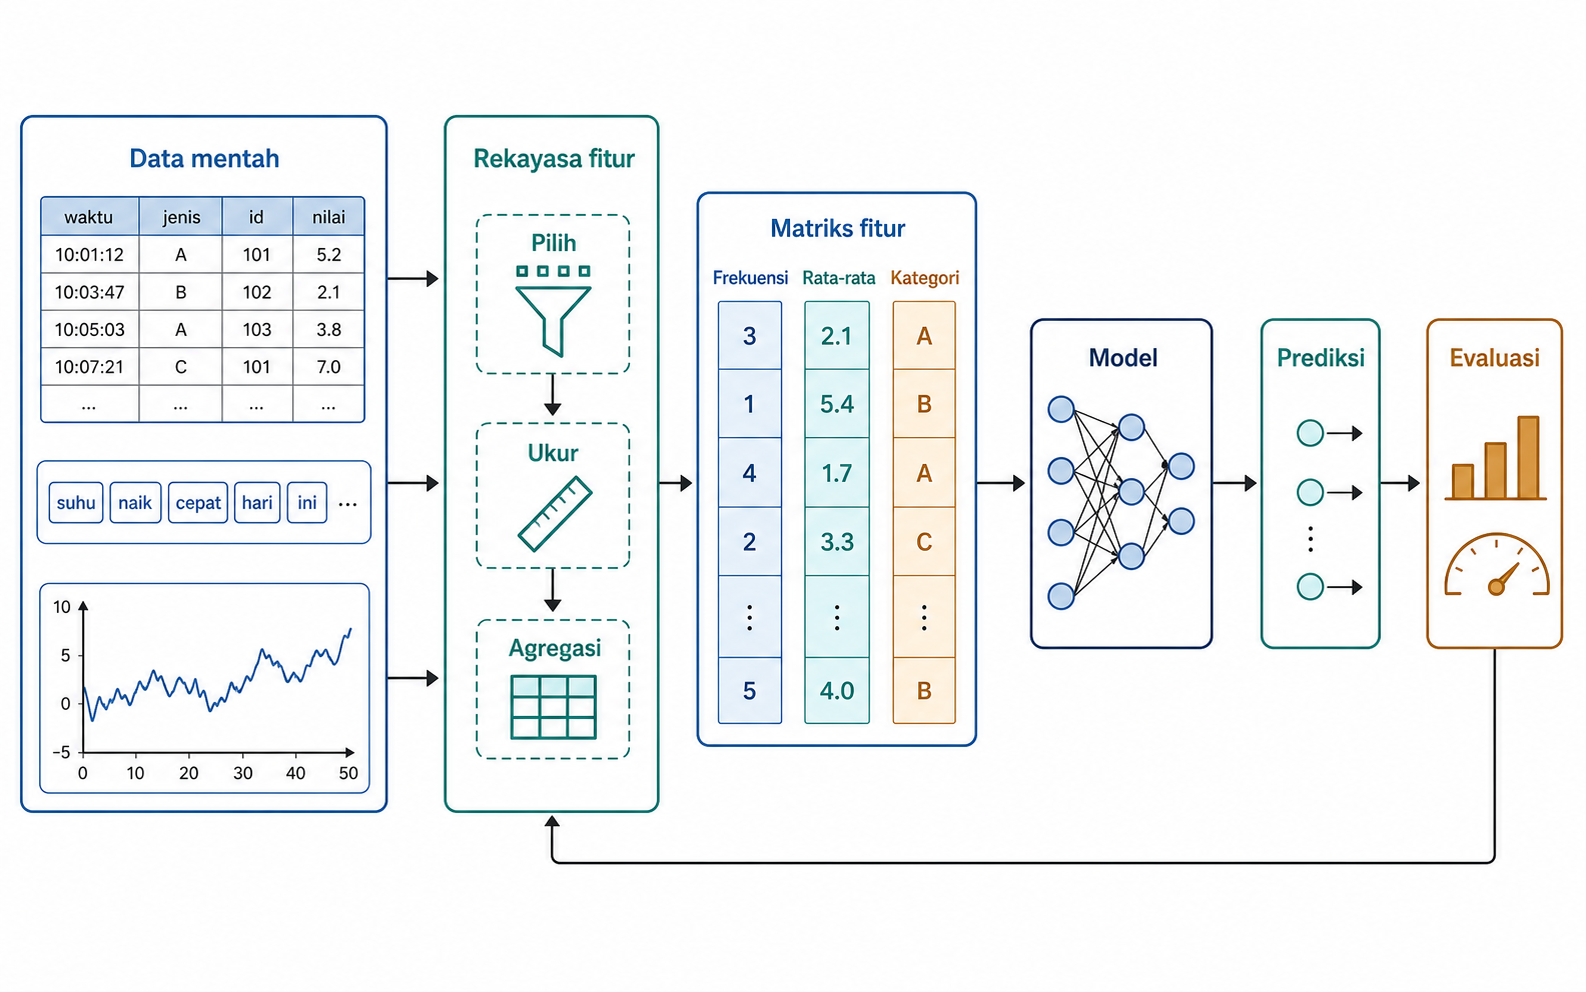
\includegraphics[width=111.6mm]{ch01-fig-1}
\caption{Posisi rekayasa fitur dalam alur \emph{machine learning}}
\label{fig:ch01-fig-1}
\end{figure}

Gambar 1.1 menempatkan rekayasa fitur di antara data mentah dan pemodelan. Posisi tersebut menegaskan bahwa catatan mentah perlu dibentuk lebih dahulu sebelum masuk ke model. Dalam praktik, alurnya juga tidak selalu bergerak satu arah. Hasil evaluasi sering mengarahkan pemeriksaan ulang terhadap unit, target, jendela waktu, atau transformasi yang dipakai.

Perubahan dari data mentah ke fitur dapat ditulis secara ringkas dengan rumus berikut.

\[
\mathbf{x} = \phi(x_{\text{raw}})
\]

Dengan \(x_{\text{raw}}\) adalah satu catatan mentah atau kumpulan catatan yang menjadi dasar satu sampel, simbol \(\phi\) melambangkan keputusan representasi yang mencakup pembersihan, agregasi, pengkodean, transformasi, pemilihan batas waktu, dan keputusan lain yang diperlukan. Hasilnya adalah \(\mathbf{x}\), yaitu representasi yang masuk ke model.

Pada data tabular, \(\mathbf{x}\) biasanya berupa vektor fitur dalam \(\mathbb{R}^d\). Namun, tidak semua masalah berakhir sebagai tabel sederhana. Teks dapat berupa urutan token, citra berupa \emph{grid} atau \emph{tensor}, jejaring berupa graf, dan sistem multimodal berupa gabungan beberapa struktur. Peta bentuk-bentuk tersebut dibahas pada Bagian 1.7. Untuk sementara, cukup pegang satu gagasan utama bahwa \(\phi\) dapat menghasilkan representasi yang dirancang manusia, representasi yang dipelajari mesin, atau gabungan keduanya.

\section{Mengapa Representasi Menentukan Hasil}\label{mengapa-representasi-menentukan-hasil}

Model hanya dapat belajar dari informasi yang sampai kepadanya. Jika suatu informasi penting tidak masuk ke dalam representasi, algoritma yang lebih kuat tidak otomatis dapat memulihkannya. Sebaliknya, ketika pola penting sudah dinyatakan dengan jelas, model yang lebih sederhana pun dapat bekerja baik pada kondisi tertentu. Hasil model bergantung pada algoritma, tetapi juga pada apa yang dibuat tampak oleh representasi.

Tabel pelanggan-bulan pada Bagian 1.1 memberi contoh langsung. Tanggal transaksi mentah memang menyimpan informasi waktu, tetapi hubungannya dengan pembelian ulang lebih mudah ditangkap setelah dihitung menjadi \passthrough{\lstinline!hari_sejak_transaksi_terakhir!}. Fitur semacam ini sering disebut \emph{recency}. Setelah selisih hari tersedia sebagai angka, kedekatan 27 Januari terhadap 1 Februari tidak lagi tersembunyi di dalam teks tanggal.

Keterbatasan tersebut mudah dilihat pada skor linear untuk target biner berikut.

\[
s = \mathbf{w}^{\top}\mathbf{x} + b, \qquad
\hat{p}(y=1\mid\mathbf{x}) = \sigma(s) = \frac{1}{1+e^{-s}}
\]

Dengan \(s\) sebagai skor linear, \(\mathbf{x}\) sebagai representasi \emph{input}, \(\mathbf{w}\) sebagai bobot yang dipelajari, dan \(b\) sebagai konstanta atau bias, fungsi sigmoid \(\sigma\) mengubah skor menjadi probabilitas kelas positif. Model hanya dapat memberi bobot pada komponen yang ada di dalam \(\mathbf{x}\). Jika informasi penting tidak pernah masuk ke \(\mathbf{x}\), pengaturan bobot sebaik apa pun tidak dapat memakai informasi tersebut.

Representasi juga membentuk cara model memperlakukan jarak, urutan, skala, kerapatan, lokalitas, dan kemiripan. \passthrough{\lstinline!StockCode!} pada Tabel 1.1, misalnya, tampak seperti kode angka-huruf. Akan tetapi, jarak antara \passthrough{\lstinline!85123A!} dan \passthrough{\lstinline!71053!} tidak mempunyai makna numerik seperti jarak antara dua harga barang. Dua produk bisa mirip karena sering dibeli bersama, bukan karena kodenya berdekatan. Karena itu, \passthrough{\lstinline!StockCode!} lebih tepat diperlakukan sebagai kategori, kelompok produk, atau \emph{embedding} yang dipelajari mesin dari pola pembelian.

Skala mempunyai pengaruh yang sama nyata. Jika satu fitur bernilai antara 0 dan 1, sedangkan fitur lain bernilai sampai jutaan, beberapa model akan lebih sensitif pada fitur berskala besar. Pada teks, urutan kata dapat membawa makna. Pada citra, ketetanggaan piksel penting. Pada graf, relasi antar-\emph{node} membawa sinyal. Setiap pilihan representasi berarti ada struktur yang dipertahankan, dan ada pula struktur yang hilang sebelum proses belajar dimulai.

Perspektif \emph{data-centric AI} menempatkan perbaikan data dan representasi sebagai tuas utama, sering kali sebelum pergantian arsitektur model. Ini bukan hukum umum. Pada data, target, dan model tertentu, representasi yang baik dapat membuat model sederhana menyaingi model kompleks dengan representasi buruk. Pada kasus lain, model kompleks tetap diperlukan. Pemeriksaan awalnya tetap sama, yaitu apakah \emph{input} model sudah menyatakan masalah dengan tepat.

Kemampuan prediksi pada data pelatihan belum cukup untuk menjadikan sebuah fitur layak dipakai. Fitur tersebut juga harus tersedia pada waktu prediksi, stabil, sesuai dengan batas biaya dan privasi, serta tidak menambah risiko bias yang tidak dapat diterima. Pertimbangan ini menentukan bagian representasi yang perlu dirancang manusia dan bagian yang dapat dipelajari mesin.

\section{Dirancang Manusia dan Dipelajari Mesin}\label{dirancang-manusia-dan-dipelajari-mesin}

Dalam buku ini, dua istilah dipakai secara sengaja, yaitu representasi yang dirancang manusia dan representasi yang dipelajari mesin. Representasi yang dirancang manusia adalah fitur yang sengaja dibuat dari pengetahuan domain, statistik, transformasi, atau aturan eksplisit. Total belanja 30 hari terakhir, jumlah \emph{invoice}, ragam produk, penanda akhir pekan, dan hari sejak transaksi terakhir merupakan contoh yang umum.

Di sisi lain, representasi yang dipelajari mesin dibentuk oleh model dari data. Bentuknya dapat berupa \emph{embedding}, vektor laten, atau aktivasi tersembunyi pada jaringan neural. Dimensinya sering tidak mempunyai nama yang mudah dijelaskan satu per satu, tetapi dapat memuat pola yang sulit dirumuskan langsung oleh manusia, terutama pada teks, citra, audio, dan graf berskala besar.

Kedua bentuk representasi sering digunakan bersama. Model pembelian ulang dapat memakai agregat transaksi yang dirancang manusia bersama \emph{embedding} produk yang dipelajari mesin. Sistem pencarian dokumen dapat memakai metadata eksplisit, seperti tanggal dan sumber dokumen, sekaligus memakai \emph{embedding} teks dari model bahasa. Letak yang tepat pada spektrum ini bergantung pada tugas, volume dan bentuk data, kebutuhan interpretabilitas, biaya komputasi, cara \emph{deployment}, serta risiko yang perlu dikendalikan.

Indeks massa tubuh memberi contoh sederhana representasi yang dirancang manusia.

\[
\text{BMI} = \dfrac{w}{h^2}
\]

Dengan \(w\) sebagai berat badan dalam kilogram dan \(h\) sebagai tinggi badan dalam meter, rumus tersebut menggabungkan dua atribut mentah menjadi satu fitur yang bermakna dalam domain kesehatan. Model dapat saja menerima berat dan tinggi secara terpisah, tetapi BMI menyatakan hubungan yang sudah dikenali manusia. Dalam hal ini, manusia tidak hanya mengubah format data. Manusia memasukkan struktur pengetahuan ke dalam representasi.

Perbedaan dua ujung spektrum tersebut diringkas pada Tabel 1.2. Kolom kiri tidak selalu lebih baik daripada kolom kanan, dan sebaliknya. Tabel ini membantu menentukan apakah suatu sinyal perlu dinyatakan secara eksplisit, dipelajari mesin dari data, atau digabungkan.

\tabeljudul{Tabel 1.2 — Perbandingan representasi yang dirancang manusia dan representasi yang dipelajari mesin}

{\def\LTcaptype{none} % do not increment counter
\par\vspace{3pt}\noindent
\begingroup\renewcommand{\arraystretch}{1.0}%
\scriptsize\linespread{1}\selectfont
\renewcommand{\_}{\textunderscore\hspace{0pt}}%
\begin{xltabular}{\linewidth}{@{}>{\raggedright\arraybackslash}p{(\linewidth-4\tabcolsep)*\real{0.192}} >{\raggedright\arraybackslash}p{(\linewidth-4\tabcolsep)*\real{0.367}} >{\raggedright\arraybackslash}p{(\linewidth-4\tabcolsep)*\real{0.441}}@{}}
\toprule

Dimensi
 & 
Representasi yang dirancang manusia
 & 
Representasi yang dipelajari mesin
 \\
\midrule
\endhead




Sumber logika & Pengetahuan domain dan aturan eksplisit & Optimisasi parameter model pada data \\
Interpretabilitas & Tinggi, setiap fitur memiliki makna yang dinyatakan & Rendah, dimensi laten jarang memiliki nama \\
Kebutuhan data & Dapat bekerja pada data kecil & Biasanya membutuhkan data besar \\
Kebutuhan komputasi & Ringan & Berat, terutama untuk pelatihan atau inferensi \emph{encoder} \\
Modalitas khas & Tabular dan data bisnis & Teks, citra, audio, graf berskala besar \\
Jenis kegagalan umum & Sinyal hilang karena tidak terpikirkan pakar & Pola semu dan bias terserap dari data \\
\bottomrule
\end{xltabular}\endgroup\par\vspace{5pt}

}

Contoh pada tabel tersebut dapat ditempatkan pada satu garis spektrum. Sisi kiri Gambar 1.2 berisi fitur yang sangat eksplisit. Bagian tengah berisi metode yang mulai belajar struktur dari data, tetapi masih sering dipakai sebagai transformasi yang terkontrol. Sisi kanan berisi representasi dari model besar yang dilatih pada data berukuran besar.

\begin{figure}[tbp]\centering
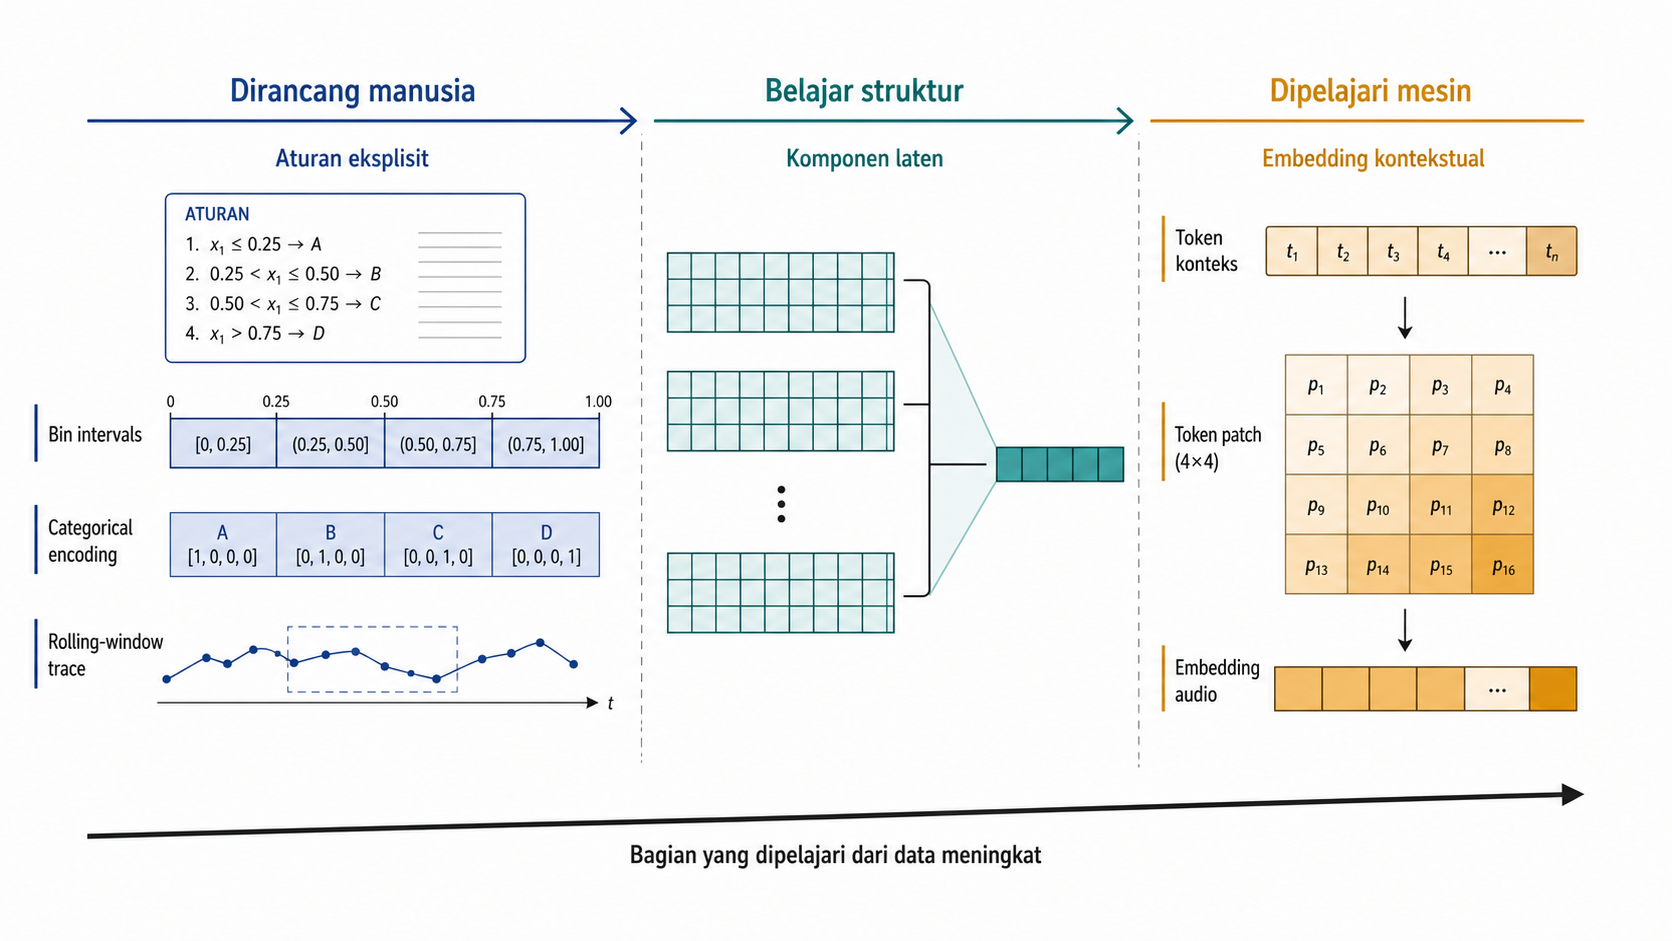
\includegraphics[width=111.6mm]{ch01-fig-2}
\caption{Spektrum representasi yang dirancang manusia sampai dipelajari mesin}
\label{fig:ch01-fig-2}
\end{figure}

Spektrum tersebut juga memberi urutan bagi pembahasan buku ini. Pembahasan dimulai dari perancangan fitur eksplisit pada data tabular, lalu bergerak ke seleksi dan reduksi, representasi menurut tipe data, representasi yang dipelajari mesin dan model \emph{pretrained}, otomatisasi, serta sintesis. Urutan ini memperluas cara memandang representasi dari bentuk yang paling eksplisit sampai bentuk yang banyak dipelajari dari data.

\begin{pendalaman}{\emph{Self-supervised learning}, manusia merancang lingkungan belajar}
Pada \emph{self-supervised learning}, manusia tidak menulis rumus fitur satu per satu. Kontribusi manusia bergeser ke perancangan tugas belajar, yang sering disebut \emph{pretext task}. Pada SimCLR (Chen et al. 2020), model belajar dari pasangan augmentasi yang seharusnya dipandang mirip. Pada Masked Autoencoders (He et al. 2022), model belajar merekonstruksi bagian \emph{input} yang disembunyikan. Dalam kedua contoh tersebut, representasi dipelajari mesin, tetapi lingkungan belajarnya tetap dirancang manusia. Posisi ini berada di sisi kanan spektrum, sekaligus memperlihatkan bahwa \emph{deep learning} tidak menghapus keputusan representasi. Bab 15 akan kembali ke tema ini ketika membahas representasi yang dipelajari mesin secara lebih luas.
\end{pendalaman}

\section{\texorpdfstring{Peran Rekayasa Fitur dalam \emph{Deep Learning}}{Peran Rekayasa Fitur dalam Deep Learning}}\label{peran-rekayasa-fitur-dalam-deep-learning}

Keberhasilan \emph{deep learning} sering membuat rekayasa fitur terdengar seperti pekerjaan lama. Pada citra, model dapat belajar pola langsung dari piksel. Pada teks, model bahasa dapat menghasilkan \emph{embedding} kontekstual tanpa daftar fitur kata yang ditulis satu per satu. Pada audio dan data sekuensial, model juga dapat belajar struktur yang dahulu memerlukan banyak aturan khusus.

Perubahan itu nyata, tetapi keputusan rekayasa fitur tetap ada. \emph{Deep learning} memindahkan sebagian pekerjaan representasi dari aturan yang dirumuskan manusia ke proses belajar mesin. Manusia masih menentukan unit sampel dan target, menetapkan jendela waktu, serta merancang tokenisasi, normalisasi \emph{input}, augmentasi, arsitektur, fungsi \emph{loss}, metadata, dan konteks yang tersedia bagi model.

Keputusan tersebut harus mengikuti keadaan saat model dipakai. Pada data berurutan waktu, misalnya, manusia tetap menetapkan unit analisis, horizon prediksi, dan batas informasi yang tersedia. Pada model fondasi, manusia menentukan dokumen atau konteks yang boleh diberikan. Karena itu, tabel pelanggan-bulan pada Bagian 1.1 harus jelas menyatakan apa yang diwakili satu baris dan informasi apa yang sah dipakai, sekalipun representasi berikutnya dipelajari oleh jaringan yang jauh lebih rumit.

\begin{pendalaman}{Rekayasa konteks untuk model fondasi}
Pada sistem berbasis LLM, penyusunan konteks berperan mirip dengan rekayasa fitur pada \emph{machine learning} klasik. Dalam \emph{retrieval-augmented generation} (Lewis et al. 2020), sistem memilih dokumen yang diberikan kepada model sebelum jawaban dihasilkan. Secara ringkas, konteks dapat ditulis sebagai \(C = q \oplus f_{\text{retrieve}}(q, \mathcal{D})\). Dalam rumus tersebut, \(q\) adalah pertanyaan atau instruksi pengguna, \(\mathcal{D}\) adalah korpus dokumen, \(f_{\text{retrieve}}\) adalah fungsi pencarian, dan \(\oplus\) adalah operasi penggabungan. Rumus itu menunjukkan bahwa \emph{query} dipadukan dengan materi yang diambil. Manusia tidak menulis fitur numerik satu per satu, tetapi tetap menentukan informasi yang sampai ke model.
\end{pendalaman}

\section{Dari Pertanyaan Prediksi ke Tabel Data untuk Model}\label{dari-pertanyaan-prediksi-ke-tabel-data-untuk-model}

Tabel pelanggan-bulan pada Bagian 1.1 baru sah dipakai jika aturan waktunya jelas. Tanpa aturan tersebut, fitur yang tampak wajar dapat berubah menjadi sumber \emph{leakage}, yaitu masuknya informasi yang belum tersedia pada saat prediksi. Pertanyaan bisnis seperti ``siapa pelanggan yang akan aktif lagi?'' perlu dipertajam menjadi pertanyaan prediksi tentang siapa yang diprediksi, kapan model diminta menjawab, dan periode mana yang dipakai untuk melihat jawabannya.

Beberapa istilah perlu dibuat jelas sejak awal:

\begin{itemize}
\tightlist
\item
  unit analisis adalah benda atau kejadian yang menjadi satu sampel, misalnya pelanggan-bulan, kunjungan pasien, perangkat-jam, transaksi, siswa-tahun ajaran, atau dokumen.
\item
  target adalah nilai atau kejadian yang ingin diprediksi untuk unit tersebut.
\item
  horizon prediksi adalah rentang waktu setelah prediksi dibuat, misalnya pembelian ulang dalam 30 hari, masuk ulang rumah sakit dalam 7 hari, atau kegagalan sensor dalam 24 jam.
\end{itemize}

Waktu prediksi ditetapkan sebagai \emph{cutoff} \(t_p\), yang pada beberapa domain juga disebut \emph{index time}. Pada Tabel 1.1, \(t_p\) adalah 1 Februari 2011. Waktu kejadian menyatakan kapan transaksi berlangsung, sedangkan waktu ketersediaan menyatakan kapan catatannya sudah dapat diketahui sistem. Keduanya dapat berbeda jika data terlambat masuk atau direvisi. Contoh ini mengasumsikan catatan langsung tersedia. Fitur hanya memakai transaksi dengan waktu kejadian di \([t_p-30\ \text{hari},t_p)\) yang sudah tersedia pada \(t_p\), sedangkan target memakai kejadian di \([t_p,t_p+30\ \text{hari})\).

\begin{figure}[tbp]\centering
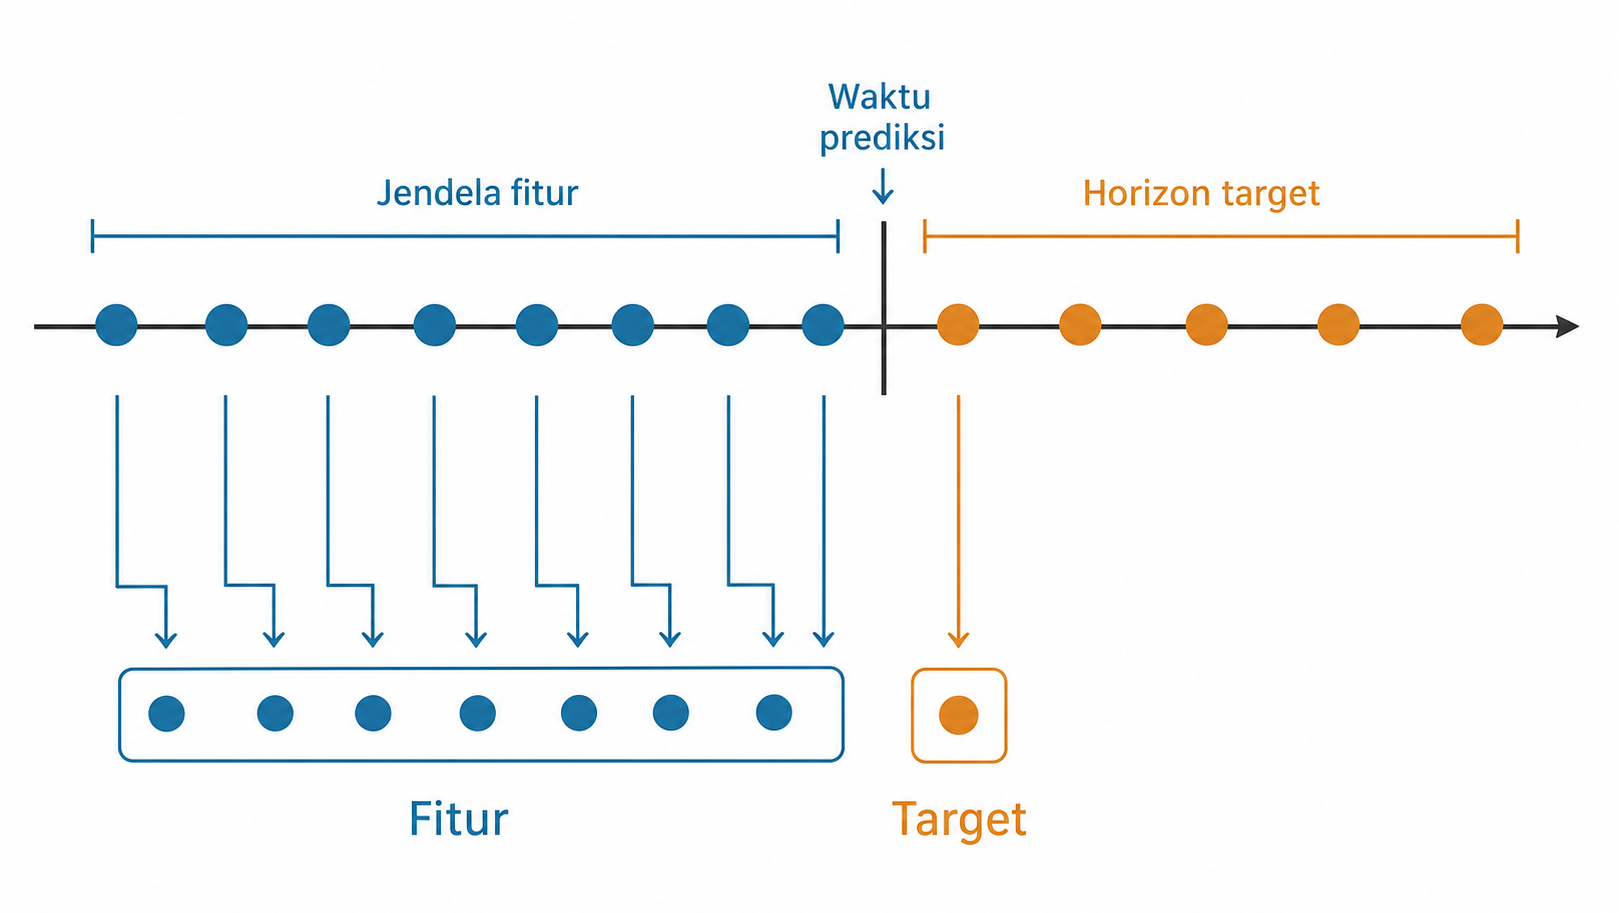
\includegraphics[width=111.6mm]{ch01-fig-3}
\caption{Tabel data untuk model sebagai potongan waktu untuk satu unit}
\label{fig:ch01-fig-3}
\end{figure}

Pada Gambar 1.3, peristiwa historis berada sebelum \emph{index time}, sedangkan zona target dimulai pada titik tersebut. Pemisahan ini menjelaskan mengapa banyak kesalahan rekayasa fitur sebenarnya merupakan kesalahan membangun tabel data untuk model. Jika total belanja dihitung dengan memasukkan transaksi pada atau setelah 1 Februari 2011, model diberi informasi dari jendela target. Evaluasi dapat terlihat baik, tetapi bukan karena model belajar memprediksi masa depan. Jawaban sudah bocor ke dalam \emph{input}.

Aturan batas waktu dapat ditulis langsung di dalam rumus agregasi. Misalkan \(v_{i,t}\) adalah nilai transaksi unit \(i\) pada waktu kejadian \(t\), \(T_i\) adalah himpunan waktu transaksi untuk unit tersebut, \(a_{i,t}\) adalah waktu ketika catatan transaksi tersedia, dan \(t_p\) adalah \emph{cutoff}. Total nilai transaksi 30 hari yang boleh dipakai sebagai fitur ditulis sebagai berikut.

\[
x_{i,\text{total,30h}} = \sum_{\substack{t \in T_i,\; t_p-30\ \text{hari} \le t < t_p \\ a_{i,t} \le t_p}} v_{i,t}
\]

Syarat \(t_p-30\ \text{hari} \le t < t_p\) membatasi waktu kejadian ke jendela fitur, sedangkan \(a_{i,t} \le t_p\) memastikan catatan tersebut sudah diketahui pada saat prediksi. Jika definisi \emph{cutoff} atau waktu ketersediaan kabur, kesalahan dapat masuk melalui agregasi transaksi, status pelanggan, riwayat sensor, log klik, atau tabel referensi yang tampak tidak berbahaya.

Karena itu, unit analisis, target, waktu prediksi, horizon prediksi, dan batas informasi perlu ditetapkan sebelum fitur dihitung. Bab 2 menjadikan aturan ini bagian dari validasi dan praktik \emph{pipeline} yang benar.

\begin{pendalaman}{\emph{Point-in-time correctness} dan \emph{feature store}}
Di sistem produksi, aturan \emph{cutoff} sering diformalkan sebagai \emph{point-in-time correctness}. Artinya, setiap nilai fitur pada data pelatihan harus direkonstruksi persis seperti nilai yang diketahui pada \emph{index time}. \emph{Feature store} seperti Feast mendukung kebutuhan ini melalui \emph{point-in-time joins}, sehingga pengambilan fitur historis pada data pelatihan mengikuti keadaan yang diketahui pada waktu tersebut. Kesamaan pelatihan dan produksi tetap menuntut definisi fitur dan jalur komputasi yang konsisten. Bab 6 kembali ke persoalan ini saat membahas \emph{as-of join} pada \emph{event log}, sedangkan Bab 17 membahasnya dari sisi infrastruktur.
\end{pendalaman}

\section{Peta Struktur Representasi}\label{peta-struktur-representasi}

Contoh utama sejauh ini berbentuk tabel. Pada \emph{machine learning} tabular, data sering disusun sebagai \emph{feature matrix} \(X \in \mathbb{R}^{n \times d}\), dengan \(n\) sampel dan \(d\) fitur. Dalam bentuk ini, sinyal terutama berada pada nilai kolom. Urutan kolom biasanya tidak bermakna secara domain, selama nama dan posisinya konsisten.

Namun, banyak data tidak hidup secara alami sebagai baris dan kolom. Pada \emph{sequence}, seperti \emph{time series}, riwayat klik, atau token teks, sinyal berada pada urutan. Kata atau kejadian yang sama dapat bermakna berbeda ketika posisinya berubah. Pada \emph{grid} atau \emph{tensor}, seperti citra, spektrogram, atau raster spasial, sinyal berada pada ketetanggaan. Piksel yang berdekatan biasanya lebih terkait daripada piksel yang jauh.

Pada set, seperti produk dalam keranjang belanja, sinyal berada pada keanggotaan dan kombinasi item, bukan pada urutan pencatatan. Pada graf, sinyal berada pada relasi tentang siapa terhubung dengan siapa, seberapa kuat hubungannya, dan pola jaringan apa yang terbentuk. Pada data multimodal, sinyal berasal dari gabungan struktur, misalnya tabel pelanggan, teks keluhan, dan gambar dokumen.

\begin{figure}[tbp]\centering
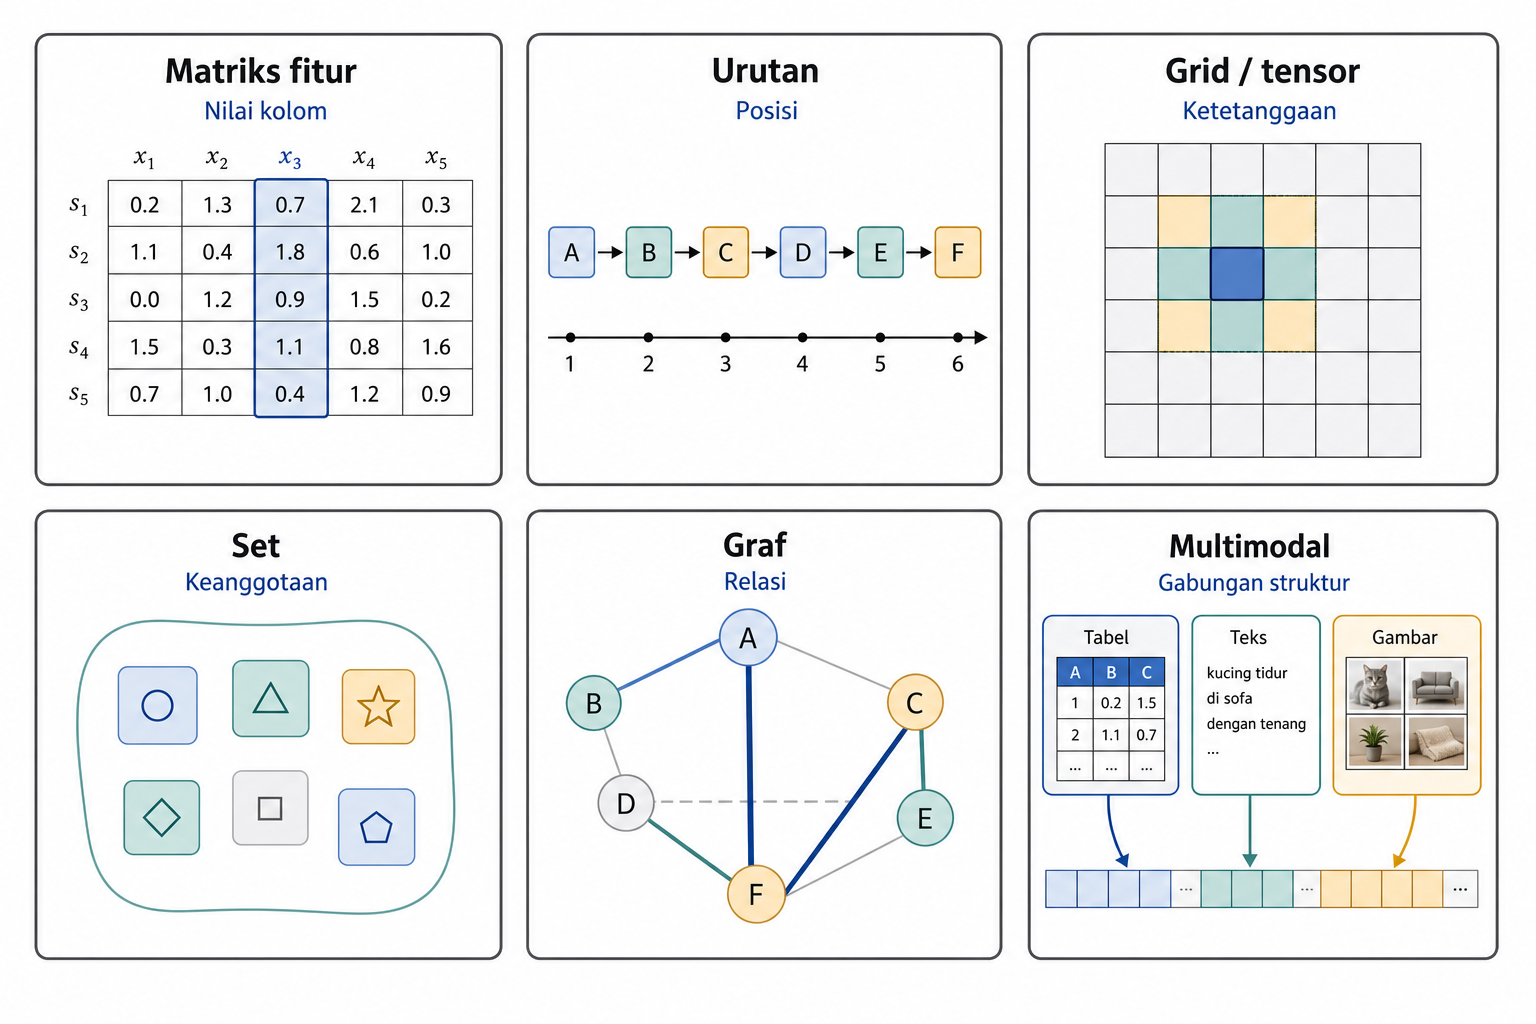
\includegraphics[width=111.6mm]{ch01-fig-4}
\caption{Peta struktur representasi}
\label{fig:ch01-fig-4}
\end{figure}

Enam panel pada Gambar 1.4 memberi peta awal, bukan taksonomi yang harus dihafal. Setiap struktur memberi petunjuk tentang strategi rekayasa fitur. Jika sinyal berada pada urutan, informasi urutan perlu dijaga. Jika sinyal berada pada relasi, fitur graf perlu dipertimbangkan. Jika sinyal berada pada gabungan modalitas, beberapa representasi harus dipertemukan tanpa menghapus struktur pentingnya. Bagian IV buku ini kembali ke peta tersebut ketika membahas data waktu, teks, citra, audio, spasial, graf, dan multimodal.

\section{\texorpdfstring{Sekilas \emph{Pipeline} dan Cara Membaca Buku}{Sekilas Pipeline dan Cara Membaca Buku}}\label{sekilas-pipeline-dan-cara-membaca-buku}

Keputusan tentang unit, target, waktu, dan struktur representasi tidak cukup dibuat sekali di awal eksperimen. Keputusan tersebut harus dijalankan dengan cara yang sama ketika data dibagi, transformasi dipasang pada data pelatihan, validasi dan \emph{test} ditransformasi, model dilatih, hasil dievaluasi, lalu sistem dipakai untuk inferensi. Rangkaian inilah yang disebut \emph{pipeline}.

Sebagai komposisi fungsi, sebuah \emph{pipeline} dapat dinyatakan dengan rumus berikut.

\[
\mathbf{X}_{\text{out}} = f_k(f_{k-1}(\cdots f_1(\mathbf{X}_{\text{raw}})))
\]

Dengan \(\mathbf{X}_{\text{raw}}\) sebagai data \emph{input}, \(f_1\) sampai \(f_k\) sebagai urutan transformasi, dan \(\mathbf{X}_{\text{out}}\) sebagai representasi akhir yang masuk ke model, rumus tersebut menekankan bahwa \emph{pipeline} merupakan satu objek berurutan. Jika transformasi di-\emph{fit} pada seluruh data sebelum pemisahan, atau jika urutannya berubah saat inferensi, maka evaluasi tidak lagi menggambarkan penggunaan nyata.

Transformasi yang belajar dari data harus di-\emph{fit} pada data pelatihan, lalu diterapkan secara konsisten pada validasi, \emph{test}, dan inferensi. Inilah inti praktik \emph{pipeline} yang benar. Bab 2 membahas \emph{leakage}, validasi, dan kontrak \passthrough{\lstinline!fit!}/\passthrough{\lstinline!transform!} secara lebih rinci. Untuk saat ini, cukup ditekankan bahwa setiap teknik fitur berada di dalam alur tersebut.

Bagian II buku ini membahas transformasi tabular, mulai dari fitur numerik, kategorikal, nilai hilang, \emph{outlier}, sampai agregasi. Bagian III membahas seleksi, reduksi, dan evaluasi fitur. Bagian IV berpindah ke representasi menurut struktur data. Bagian V membahas representasi yang dipelajari mesin dan model \emph{pretrained} pada Bab 15, otomatisasi pada Bab 16, lalu sintesis dalam \emph{pipeline} produksi pada Bab 17.

Untuk membaca secara selektif, Bab 1 dan Bab 2 sebaiknya dibaca terlebih dahulu karena keduanya membentuk bahasa bersama tentang representasi dan validasi. Sebelum melaporkan hasil eksperimen, baca Bab 9. Setelah itu, pembaca dapat langsung menuju bab yang sesuai dengan tipe data, misalnya tabular, waktu, teks, citra, audio, spasial, graf, atau multimodal.

Spektrum pada Bagian 1.4 tetap menjadi peta keputusan. Pada data kecil, domain yang diatur ketat, atau model yang harus dijelaskan, representasi yang dirancang manusia sering menjadi titik awal yang kuat. Pada data tak terstruktur berskala besar dengan pola kompleks, representasi yang dipelajari mesin sering lebih sesuai. Dalam sistem produksi, jawaban yang banyak muncul adalah bentuk hibrid tempat fitur eksplisit, \emph{embedding}, aturan waktu, dan transformasi \emph{pipeline} hidup bersama.

\begin{sintesis}

Fitur terbentuk dari keputusan representasi. Penyusunannya menetapkan unit yang diprediksi, target yang dikejar, waktu prediksi, informasi yang sah dipakai, dan struktur data yang perlu dipertahankan. Satu atribut dapat menjadi beberapa fitur, satu fitur gabungan, atau tidak dipakai sama sekali.

Di sepanjang spektrum representasi, manusia dan mesin berbagi pekerjaan. Representasi yang dirancang manusia memberi interpretabilitas, efisiensi data, dan kontrol domain. Representasi yang dipelajari mesin memberi fleksibilitas besar, terutama pada modalitas kompleks dan data berskala besar, tetapi menuntut data, komputasi, dan pemeriksaan risiko yang lebih serius. Pada setiap masalah, bagian dari \(\phi\) perlu dipilih secara sadar, baik untuk dinyatakan manusia, dipelajari mesin, maupun digabungkan.

Setiap teknik pada bab-bab berikutnya, dari \emph{scaling} sampai \emph{embedding}, merupakan cara memilih \(\phi\) yang mengubah data mentah menjadi \emph{input} model. Model mengolah representasi yang dibangun untuk tugasnya.

\end{sintesis}

\begin{bacaan}

\begin{itemize}
\tightlist
\item
  Chip Huyen, ``Building a Generative AI Platform'' --- \url{https://huyenchip.com/2024/07/25/genai-platform.html}. Menyamakan konstruksi konteks (RAG, tool use) dengan rekayasa fitur pada era model fondasi.
\item
  Eugene Yan, ``Feature Stores: A Hierarchy of Needs'' --- \url{https://eugeneyan.com/writing/feature-stores/}. Memandang fitur sebagai aset terkelola, termasuk \emph{point-in-time correctness} dan konsistensi latih--saji.
\item
  Tecton, ``What Is a Feature Platform?'' --- \url{https://www.tecton.ai/blog/what-is-a-feature-platform/}. Arsitektur platform fitur di lingkungan produksi.
\item
  Feast, dokumentasi \emph{feature store} --- \url{https://docs.feast.dev/}. Realisasi \emph{as-of join} dan \emph{point-in-time correctness}.
\item
  Google, Machine Learning Crash Course --- \url{https://developers.google.com/machine-learning/crash-course}. Pengantar praktis representasi dan fitur.
\item
  Data-Centric AI Resource Hub --- \url{https://datacentricai.org/}. Gerakan yang menempatkan perbaikan data sebagai tuas utama performa model.
\end{itemize}

\end{bacaan}

\rujukanheading

\protect\phantomsection\label{refs}
\begin{CSLReferences}{1}{1}
\bibitem[\citeproctext]{ref-chen2020simclr}
Chen, Ting, Simon Kornblith, Mohammad Norouzi, and Geoffrey Hinton. 2020. {``A Simple Framework for Contrastive Learning of Visual Representations.''} \emph{Proceedings of the 37th International Conference on Machine Learning (ICML)}. \url{https://arxiv.org/abs/2002.05709}.

\bibitem[\citeproctext]{ref-he2022mae}
He, Kaiming, Xinlei Chen, Saining Xie, Yanghao Li, Piotr Dollár, and Ross Girshick. 2022. {``Masked Autoencoders Are Scalable Vision Learners.''} \emph{Proceedings of the IEEE/CVF Conference on Computer Vision and Pattern Recognition (CVPR)}. \url{https://arxiv.org/abs/2111.06377}.

\bibitem[\citeproctext]{ref-lewis2020rag}
Lewis, Patrick, Ethan Perez, Aleksandra Piktus, et al. 2020. {``Retrieval-Augmented Generation for Knowledge-Intensive {NLP} Tasks.''} \emph{Advances in Neural Information Processing Systems (NeurIPS)}. \url{https://arxiv.org/abs/2005.11401}.

\end{CSLReferences}

% ==========================================================================
% ch02.tex — dihasilkan otomatis dari website/chapters/ch02.qmd
% Boleh disunting manual. 'sync' hanya menimpa bila .qmd berubah DAN .tex
% belum disunting; kalau keduanya berubah, dilewati (pakai --force).
% qmd-sha1: ce2e10931ece
% tex-sha1: ca8fad5a530d
% ==========================================================================
% >>>>> ISI OTOMATIS (jangan hapus baris ini) >>>>>
\chapter{Pipeline, Validasi, dan Data Leakage}\label{pipeline-validasi-dan-data-leakage}

Mengembangkan model pembelajaran mesin yang akurat di laboratorium komputasi adalah satu hal, namun memastikannya tetap tangguh saat menghadapi aliran data dunia nyata adalah tantangan yang sepenuhnya berbeda. Di lingkungan produksi, model sering kali runtuh bukan karena kelemahan arsitektur algoritmanya, melainkan karena kegagalan menjaga konsistensi prapemrosesan data. Ketika kita menghitung parameter transformasi secara ceroboh, informasi dari masa depan atau dari data uji dapat bocor ke dalam proses pelatihan. Kebocoran data (\emph{data leakage}) ini menciptakan ilusi performa akademis yang luar biasa, namun berujung pada kegagalan total saat model dihadapkan pada kenyataan operasional.

Bab ini membahas bagaimana mengarantina data secara ketat sejak awal. Melalui penguasaan kontrak \emph{fit} dan \emph{transform}, perancangan pemisahan data (\emph{data split}) yang valid secara temporal maupun berkelompok, serta pengikatan seluruh operasi prapemrosesan ke dalam sebuah objek \emph{pipeline}, kita dapat membangun sistem yang kebal terhadap kebocoran informasi. Menguasai kedisiplinan ini adalah langkah pertama yang memisahkan seorang akademisi eksperimental dari seorang praktisi pembelajaran mesin yang andal di industri.

\section{Fit dan Transform: Pipeline sebagai Kontrak Pelatihan dan Inferensi}\label{fit-dan-transform-pipeline-sebagai-kontrak-pelatihan-dan-inferensi}

Transformasi data dalam \emph{machine learning} menuntut konsistensi absolut antara tahap pelatihan dan tahap inferensi. Model mengharapkan fitur dari data masa depan diubah menggunakan aturan dan metrik yang sama persis dengan data pelatihannya. Konsistensi ini adalah inti dari praktik \emph{pipeline} yang benar.

Kunci untuk menjaga konsistensi ini terletak pada dua mekanisme utama: \emph{fit} dan \emph{transform}. Tahap \emph{fit} adalah proses pengamatan dan perhitungan parameter dari kumpulan data pelatihan; sistem membaca data latih untuk menetapkan acuan numerik seperti nilai rata-rata, standar deviasi, atau batas rentang kategori. Setelah itu, tahap \emph{transform} mengambil alih untuk mengaplikasikan parameter hasil \emph{fit} tersebut ke dalam data observasi demi menghasilkan matriks fitur akhir. Aturannya sangat tegas: perhitungan parameter pada tahap \emph{fit} hanya boleh menyentuh data pelatihan. Setelah parameter ini dikunci, operasi \emph{transform} menggunakan acuan yang sama untuk memodifikasi data pelatihan, data validasi, maupun data inferensi di masa depan.

\begin{figure}[htbp]\centering
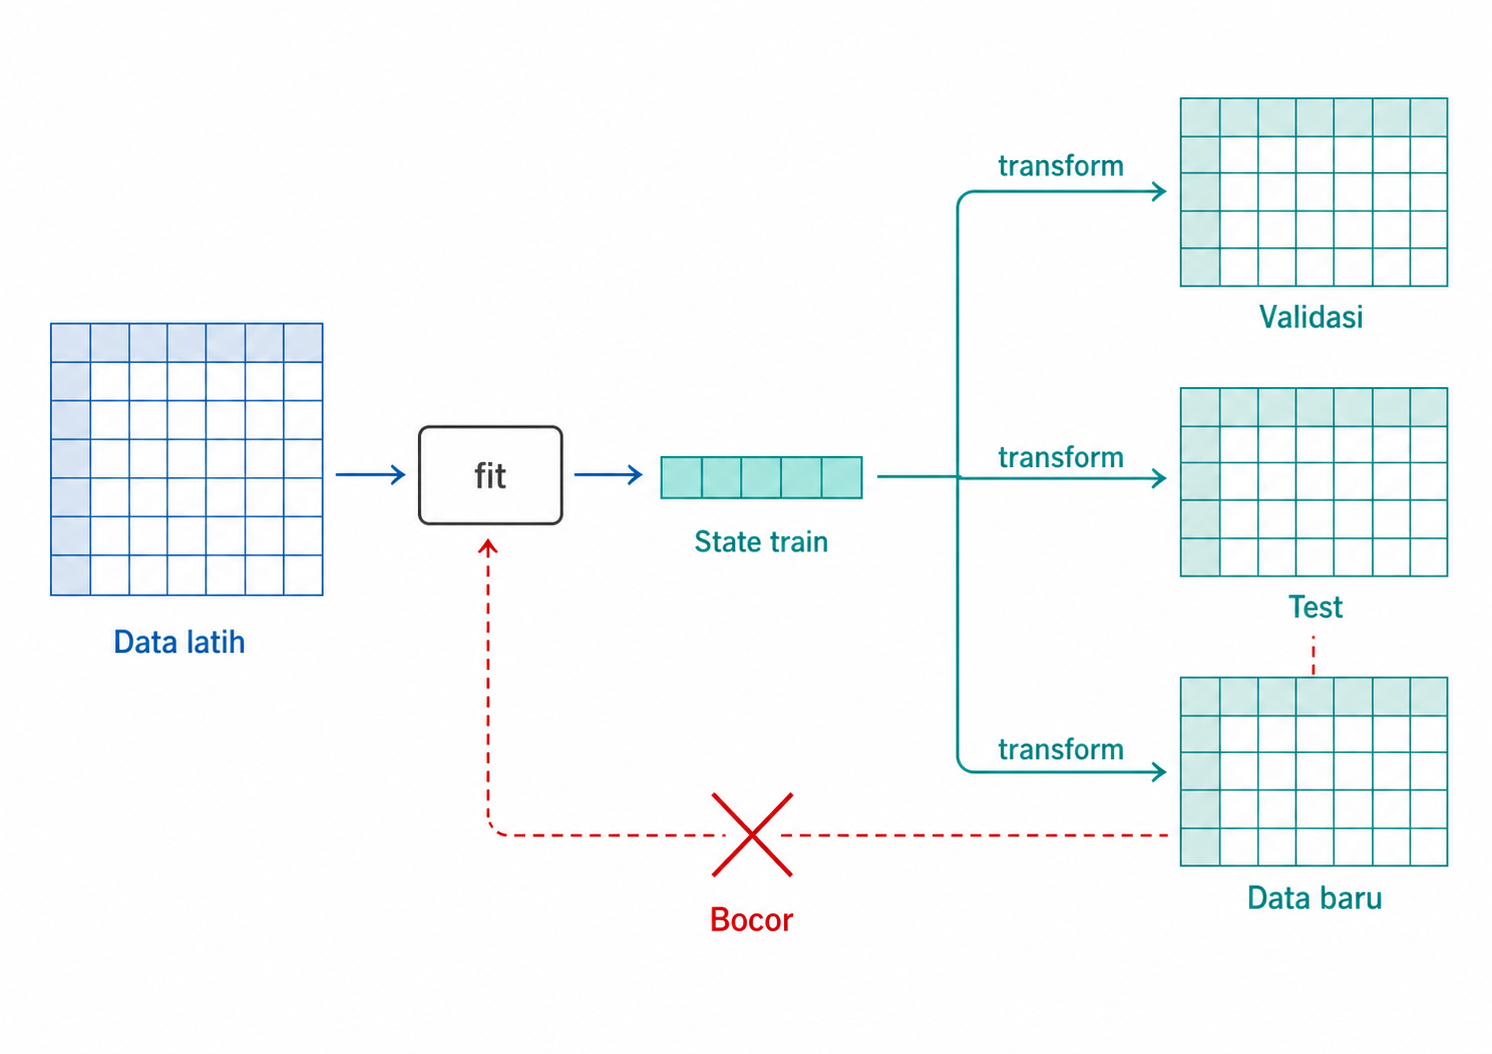
\includegraphics[width=\linewidth,height=0.72\textheight,keepaspectratio]{ch02-fig-1}
\caption{Ilustrasi Tabel ke Matriks Fitur pada Proses Fit dan Transform}
\label{fig:ch02-fig-1}
\end{figure}

Secara konseptual, kontrak transformasi ini direpresentasikan dengan rumusan:

\[ X_{transform} = T(X_{raw}; \theta_{pelatihan}) \]

Di mana \(X_{raw}\) adalah data observasi mentah yang akan diubah, \(T\) mewakili fungsi transformasi, dan \(\theta_{pelatihan}\) melambangkan parameter yang diekstraksi secara eksklusif dari data pelatihan. Informasi dari data pengujian atau inferensi dilarang bocor ke dalam \(\theta_{pelatihan}\).

Misalkan kita menstandardisasi sebuah fitur. Tahap \emph{fit} menemukan fitur tersebut memiliki rata-rata 5,0 dengan standar deviasi 2,0 pada populasi data pelatihan. Beberapa bulan kemudian, data inferensi baru masuk dengan rata-rata aktual populasi 7,0. Kita tetap wajib mengurangi setiap nilai pada data inferensi dengan 5,0 dan membaginya dengan 2,0. Acuan distribusi masa pelatihan mutlak dipertahankan.

Jika kita memanggil fungsi \emph{fit} ulang pada kelompok data inferensi, kita telah menghitung acuan yang baru. Makna fitur akan melenceng dari standar awalnya dan model akan salah menafsirkan nilai tersebut. Fenomena ini disebut \emph{training-serving skew}, sebuah anomali yang membuat akurasi model menjadi berantakan di lingkungan produksi meskipun performa pelatihannya tinggi.

Mengingat manipulasi transformasi secara manual rentan memicu kelalaian, kita mengikat proses ini ke dalam sebuah \emph{pipeline}. Objek tunggal ini menyatukan operasi pemrosesan data dan algoritma untuk membungkus kontrak \emph{fit} dan \emph{transform} secara terpusat. Saat dilatih, \emph{pipeline} membatasi pencarian parameter murni pada himpunan data latih. Objek ini kemudian menyalurkan parameter tersebut ke tahap \emph{transform} untuk menangani data baru secara konsisten.

Praktik rekayasa modern melengkapi abstraksi \emph{pipeline} ini dengan berbagai utilitas. Ekosistem pustaka seperti scikit-learn menyediakan konfigurasi \passthrough{\lstinline!set_output(transform='pandas')!} agar setiap \emph{transformer} mengembalikan \emph{DataFrame} pandas, bukan \emph{array} tanpa label. Fitur ini menjaga nama kolom tetap utuh sepanjang rantai transformasi untuk memudahkan pelacakan asal-usul fitur. Untuk eksekusi skala besar, pengembang juga dapat memanfaatkan mekanisme \emph{caching} lewat parameter \passthrough{\lstinline!memory!} guna mencegah komputasi ulang \emph{transformer} pada objek yang sama. Integrasi antara disiplin kontrak transformasi dan utilitas kode ini memastikan seluruh representasi data selaras dan stabil.

\section{Transformer yang Dapat Digunakan Ulang, Serialisasi, dan Random State}\label{transformer-yang-dapat-digunakan-ulang-serialisasi-dan-random-state}

Banyak praktisi merangkai pemrosesan data sebagai rentetan skrip \emph{ad-hoc}. Mereka menambal nilai kosong, mengubah skala, atau mengevaluasi fitur secara langsung pada tabel utama. Sebagai contoh, saat mereka memutuskan untuk menyaring kolom berdasarkan kalkulasi rasio nilai yang kosong (\(r_{missing} = \frac{N_{na}}{N_{total}}\)). Dalam perumusan tersebut, \(r_{missing}\) adalah rasio kekosongan data pada suatu fitur, \(N_{na}\) mewakili jumlah baris yang tidak memiliki nilai, dan \(N_{total}\) adalah populasi observasi keseluruhan. Keputusan mengeksekusi modifikasi \emph{ad-hoc} di luar kerangka komputasi utama seperti ini cenderung rapuh dan membuka celah kesalahan. Hasilnya, muncul ketidaksesuaian struktural antara data latih dan wujud data inferensi aktual ketika model berjalan di lingkungan produksi.

Setiap operasi modifikasi fitur wajib dikapsulkan ke dalam sebuah \emph{transformer}. Objek mandiri ini memisahkan secara tegas fase pembelajaran parameter internal (\passthrough{\lstinline!fit!}) dari fase modifikasi data itu sendiri (\passthrough{\lstinline!transform!}). Parameter yang dipelajari dari \(N_{total}\) baris - seperti batas rentang normalisasi atau nilai imputasi - terkunci aman dari risiko intervensi manual yang tidak disengaja.

\begin{figure}[htbp]\centering
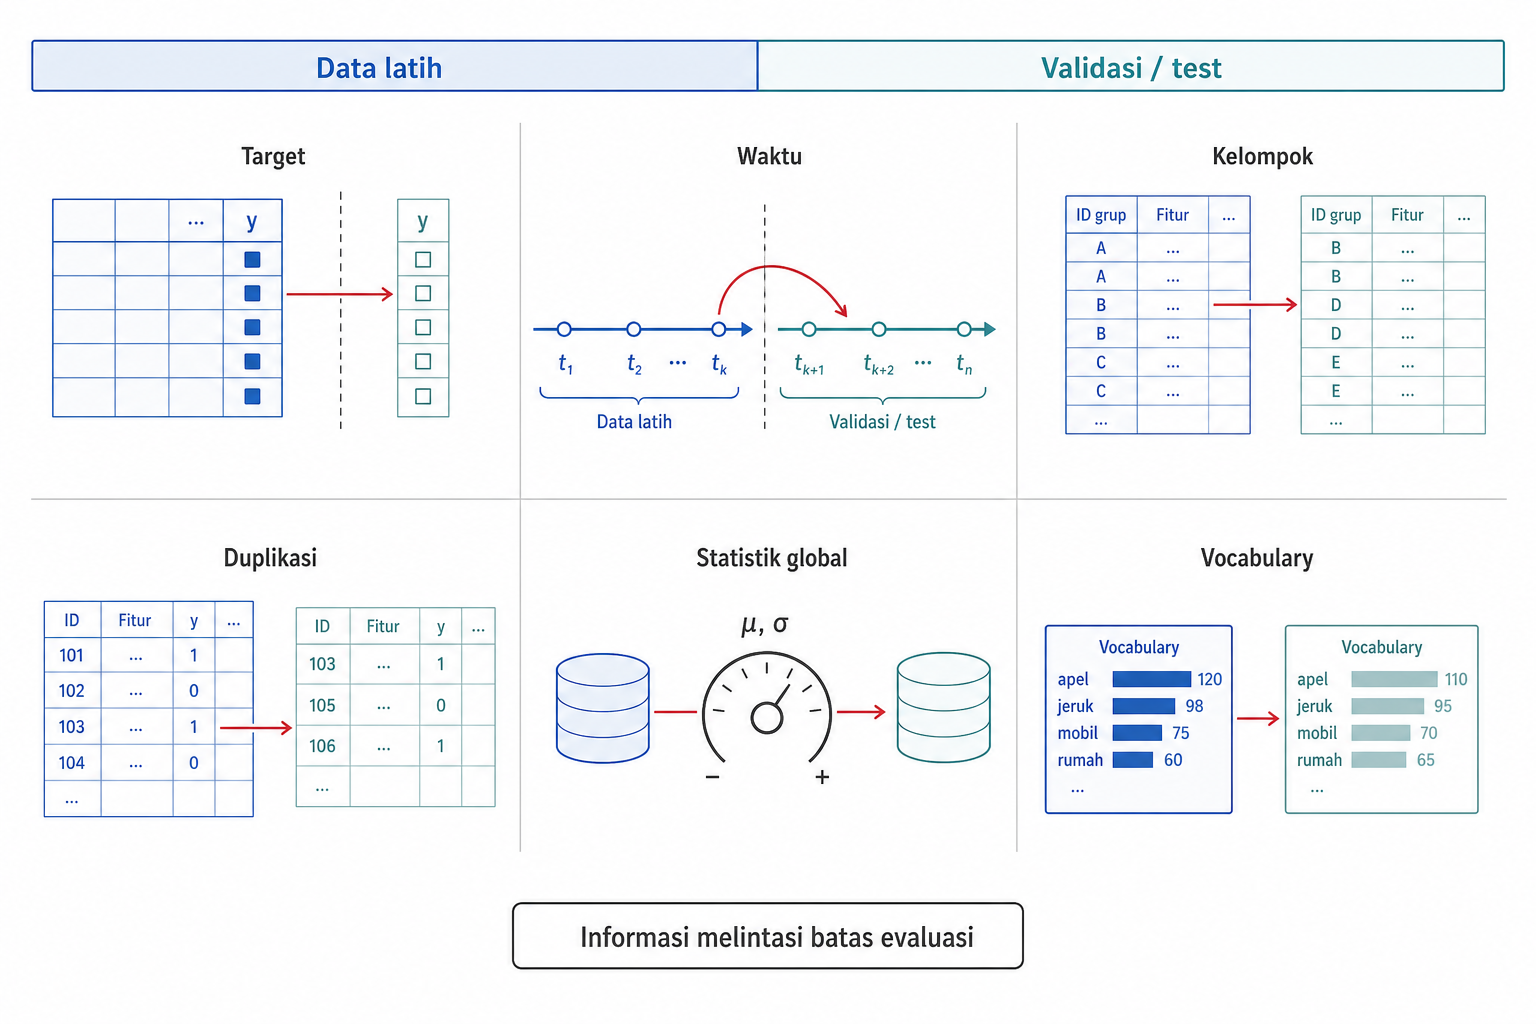
\includegraphics[width=\linewidth,height=0.72\textheight,keepaspectratio]{ch02-fig-2}
\caption{Siklus Eksplorasi-Ekstraksi-Seleksi dalam Objek Transformer Mandiri}
\label{fig:ch02-fig-2}
\end{figure}

\textbf{Serialisasi dan Persistensi Model.}\label{serialisasi-dan-persistensi-model}

Objek \emph{transformer} yang telah menampung parameter dapat disimpan secara permanen. Proses mentransfer wujud komputasi dari memori menuju berkas fisik ini dinamakan serialisasi. Praktik rekayasa fitur modern berpegang pada beberapa standar. Jika bekerja di ekosistem Python, format \emph{native} seperti pustaka \passthrough{\lstinline!joblib!} atau \passthrough{\lstinline!pickle!} merupakan spesifikasi resmi yang dianjurkan. Namun, jika algoritma diproyeksikan untuk beroperasi di luar kerangka Python (misalnya pada arsitektur mesin C++ atau Java), spesifikasi ONNX (\emph{Open Neural Network Exchange}) sebagai format lintas bahasa harus diprioritaskan. Berkas biner hasil serialisasi ini kelak dikirimkan mendampingi model prediktif utama ke \emph{server} produksi, demi menjamin data baru diproses dengan takaran yang mutlak sama dengan tahapan pelatihan.

\textbf{Pipeline Khusus untuk Resampling.}\label{pipeline-khusus-untuk-resampling}

Data yang tidak seimbang (\emph{imbalanced data}) memunculkan tantangan struktural terhadap kontrak desain \emph{transformer}. Algoritma \emph{resampling} seperti SMOTE secara aktif mengubah jumlah baris sampel pada titik eksekusinya. Dalam hal ini, kita harus menghindari skema \emph{pipeline} standar karena ia mengasumsikan konsistensi jumlah baris secara persis. Memaksakan penerapan algoritma \emph{resampling} pada kerangka bawaan ini sering kali memicu perubahan matriks inferensi yang keliru. Solusinya adalah menggunakan \emph{pipeline} ekstensi seperti \passthrough{\lstinline!imblearn.pipeline.Pipeline!} yang memastikan penambahan sampel sintetis (\passthrough{\lstinline!fit_resample!}) hanya aktif selama berlangsungnya fase pelatihan. Tahapan tersebut secara otomatis diabaikan pada saat inferensi berjalan tunggal (\passthrough{\lstinline!transform!}). Tanpa penyekatan fungsional ini, sampel tiruan akan meluber ke dalam himpunan data pengujian murni, sehingga memproduksi estimasi performa akurasi yang tidak valid.

\textbf{Pengendalian Keacakan (Random State).}\label{pengendalian-keacakan-random-state}

Keterulangan rekayasa fitur bertumpu pada kontrol elemen keacakan matematis. Generator nomor acak mengoperasikan proses sentral seperti pemisahan dataset awal, dan pengendaliannya (\emph{random state}) menyusun fondasi keakuratan pengujian silang (\emph{cross-validation}). Untuk objek pemisah (\emph{splitter}), memberikan nilai bilangan bulat (\emph{integer}) secara langsung merupakan langkah teraman yang menggaransi struktur lipatan pengujian akan selalu identik ketika teknisi membandingkan kinerja dari beberapa model. Sementara itu, untuk \emph{estimator} atau \emph{transformer}, menyerahkan instans objek \passthrough{\lstinline!RandomState!} memastikan tiap siklus lipatan data menerima urutan acak yang independen serta solid secara statistik. Terakhir, kita wajib menghindari penyetelan angka acak (\emph{seed}) secara global pada tingkat \emph{runtime} pustaka numerik, karena berisiko menimbulkan komplikasi algoritma sekunder yang sulit dilacak pada landasan kode berskala luas.

\section{\texorpdfstring{Taksonomi \emph{Data Leakage}}{Taksonomi Data Leakage}}\label{taksonomi-data-leakage}

Validasi model \emph{machine learning} sering kali menghasilkan metrik performa tinggi di tahap awal, namun gagal saat diuji pada data riil. Penyebab utama kegagalan ini adalah \emph{data leakage} (kebocoran data). Kondisi ini terjadi ketika informasi dari himpunan pengujian atau variabel target masuk ke dalam proses pelatihan. Mesin tidak lagi mempelajari pola generalisasi, melainkan menyontek jawaban dari fitur yang bocor.

\begin{figure}[htbp]\centering
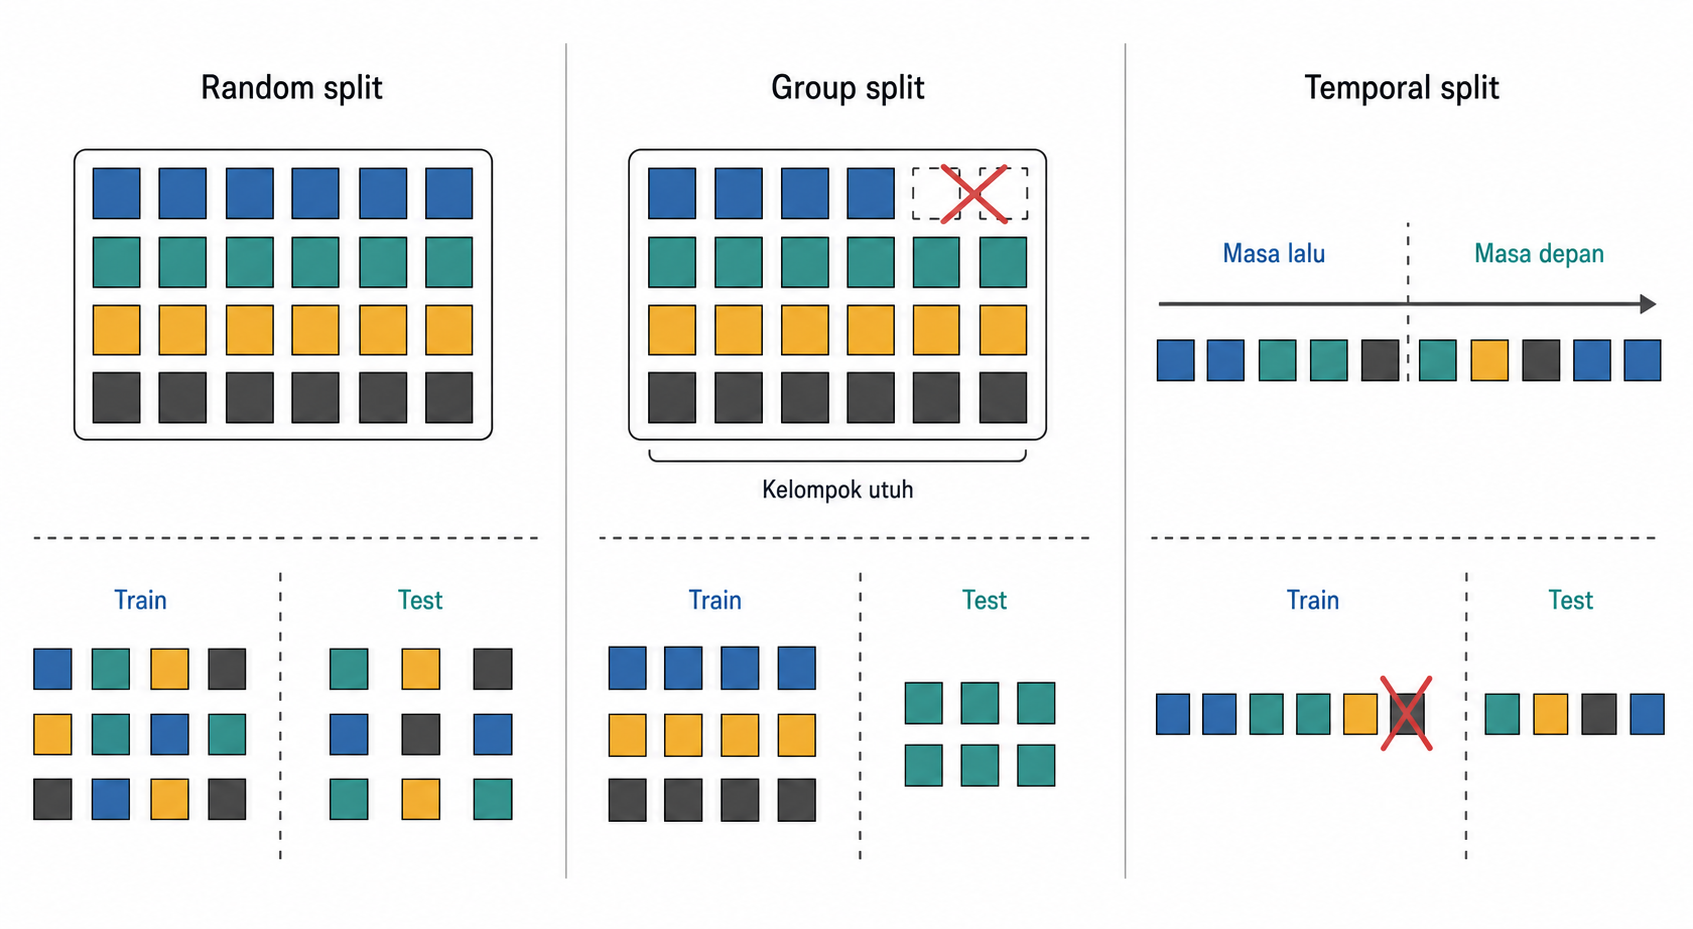
\includegraphics[width=\linewidth,height=0.72\textheight,keepaspectratio]{ch02-fig-3}
\caption{Mekanisme Data Leakage: Masuknya Informasi Pengujian ke Latih}
\label{fig:ch02-fig-3}
\end{figure}

Terdapat enam tipe utama kebocoran data yang dapat merusak validitas model.

Tipe pertama adalah kebocoran target (\emph{target leakage}). Kebocoran ini muncul saat atribut fitur bertindak sebagai proksi target, atau nilainya baru direkam setelah kejadian target berlangsung, sehingga fitur tersebut secara logis tidak tersedia pada momen prediksi di lapangan. Sebagai contoh, memprediksi pembatalan layanan pelanggan menggunakan fitur ``tanggal penutupan akun'', yang tentu saja baru terisi setelah target mencapai status batal. Kebocoran target umumnya menghasilkan fitur dengan metrik kepentingan yang sangat anomali. Secara matematis, perhitungan dasar \emph{permutation feature importance} mengukur penurunan performa saat satu fitur diacak dengan formula konseptual \(I_j = \text{Error}(f(X_{\pi(j)}), Y) - \text{Error}(f(X), Y)\). Di sini \(I_j\) adalah tingkat kepentingan fitur ke-\(j\), \(\text{Error}\) adalah fungsi kerugian dari prediksi model \(f\), \(X\) adalah matriks fitur asli, \(Y\) adalah target aktual, dan \(X_{\pi(j)}\) adalah matriks fitur dengan nilai pada kolom ke-\(j\) yang diacak. Jika fitur memuat \emph{target leakage}, pengacakan kolom tersebut akan menghancurkan bocoran jawaban, sehingga nilai \emph{error} melonjak drastis dan skor \(I_j\) menjadi terlampau dominan.

Tipe kedua adalah kontaminasi latih-uji (\emph{train-test contamination}). Fase pelatihan secara tidak sengaja menyerap informasi statistik dari himpunan data uji karena proses agregasi fitur dilakukan mendahului tahap pemisahan data. Kasus klasiknya adalah menghitung rata-rata seluruh populasi data untuk imputasi nilai kosong, baru kemudian membelah data menjadi himpunan latih dan uji; parameter rata-rata tersebut sudah tidak steril karena dipengaruhi distribusi data uji. Pencegahannya adalah dengan melakukan seluruh kalkulasi agregat eksklusif pada himpunan latih, lalu diaplikasikan searah ke himpunan uji.

Tipe ketiga adalah kebocoran temporal (\emph{temporal leakage}). Pada deret waktu dan data historis, penggunaan observasi masa depan untuk menyusun prediksi kejadian masa lalu akan membalikkan urutan kausalitas. Contohnya memisahkan riwayat transaksi perbankan secara acak tanpa mempertahankan urutan waktu, sehingga model mengeksploitasi pola transaksi hari Jumat untuk menebak probabilitas penipuan di hari Selasa sebelumnya.

Tipe keempat adalah kebocoran antar-kelompok (\emph{between-group leakage}). Sebagian data memuat unit observasi berkelompok dengan korelasi kuat antar-barisnya. Memecah data secara acak murni akan mendistribusikan anggota dari entitas yang sama ke dalam himpunan latih dan uji secara bersamaan. Jika rekam medis menyimpan sepuluh baris riwayat kunjungan dari pasien yang sama lalu disebar melintasi batas himpunan, model akan menghafalkan identitas unik pasien alih-alih belajar mendiagnosis gejala umum.

Tipe kelima adalah kebocoran \emph{embedding} (\emph{embedding leakage}). Praktik modern sering memanfaatkan model praletih untuk mengubah data mentah menjadi vektor padat. Jika adaptasi lapisan model dilakukan pada seluruh korpus teks proyek sebelum pemisahan data, vektor fitur latih sudah terpengaruh secara matematis oleh konteks semantik dokumen pengujian.

Terakhir, tipe keenam adalah kebocoran penyesuaian LLM (\emph{LLM fine-tuning leakage}). Pada komputasi teks skala masif, dokumen pengujian tanpa sengaja masuk ke dalam tumpukan data prapelatihan atau dataset instruksi (\emph{instruction-tuning}). Akibatnya, LLM dapat mencetak akurasi evaluasi nyaris sempurna pada dataset tolok ukur karena baris kode evaluasi tersebut telah terekspos sebelumnya, mengubah pengujian generalisasi menjadi sekadar tes hafalan.

\section{Mengapa Leakage Bermula pada Tahap Rekayasa Fitur}\label{mengapa-leakage-bermula-pada-tahap-rekayasa-fitur}

Kebocoran data (\emph{data leakage}) hampir tidak pernah bersumber dari algoritma \emph{machine learning}. Algoritma pada dasarnya hanyalah pengoptimal matematis yang menyesuaikan bobot berdasarkan pola pada set data yang diterimanya. Sebaliknya, kebocoran informasi justru terjadi jauh lebih awal, yakni pada tahap persiapan data dan rekayasa fitur. Saat kita mengubah tabel struktural mentah menjadi matriks representasi numerik, risiko masuknya informasi dari himpunan uji (\emph{test set}) ke dalam parameter pelatihan (\emph{training set}) menjadi sangat tinggi.

Tujuan utama rekayasa fitur adalah mengekstraksi representasi data yang membuat pola target lebih mudah dikenali oleh model. Karena proses transformasi ini sering menuntut kalkulasi pada tingkat populasi, kebocoran data umumnya berasal dari praktik transformasi yang tak sengaja memecah batas isolasi partisi. Praktik pertama adalah perhitungan statistik agregat yang membuat turunan fitur lintas observasi secara bersamaan, seperti menghitung rata-rata pengeluaran warga dalam satu wilayah atau persentase rasio keberhasilan historis. Praktik kedua adalah penerapan transformasi skala secara menyeluruh, misalnya menggunakan \emph{Standard Scaler} ke seluruh tabel sebelum melakukan proses pemotongan data (\emph{splitting}). Praktik ketiga adalah komputasi imputasi dan evaluasi atribut, di mana ukuran metrik kriteria seleksi atau statistik pengisian nilai kosong dihitung menggunakan seluruh observasi gabungan, alih-alih diukur murni dari himpunan latih.

Sebagai contoh konkret, dalam menangani atribut tak lengkap, kita umumnya menghitung rasio nilai yang hilang (\(r_{missing} = \frac{N_{missing}}{N_{total}}\)) untuk memutuskan kelayakan suatu fitur. Di sini, \(r_{missing}\) adalah proporsi kekosongan data, \(N_{missing}\) merupakan jumlah observasi yang tidak memiliki nilai, dan \(N_{total}\) adalah total baris. Apabila penyebut \(N_{total}\) mencakup jumlah observasi gabungan sebelum \emph{dataset} dipisah, maka keputusan seleksi (misalnya mencabut fitur jika \(r_{missing} > 0.4\)) telah dipengaruhi oleh kondisi data pengujian. Ketika pemotongan baris baru dilakukan setelah transformasi ini, nilai atau struktur ruang fitur pada himpunan latih sudah secara permanen terjangkiti informasi dari masa depan.

\begin{figure}[htbp]\centering
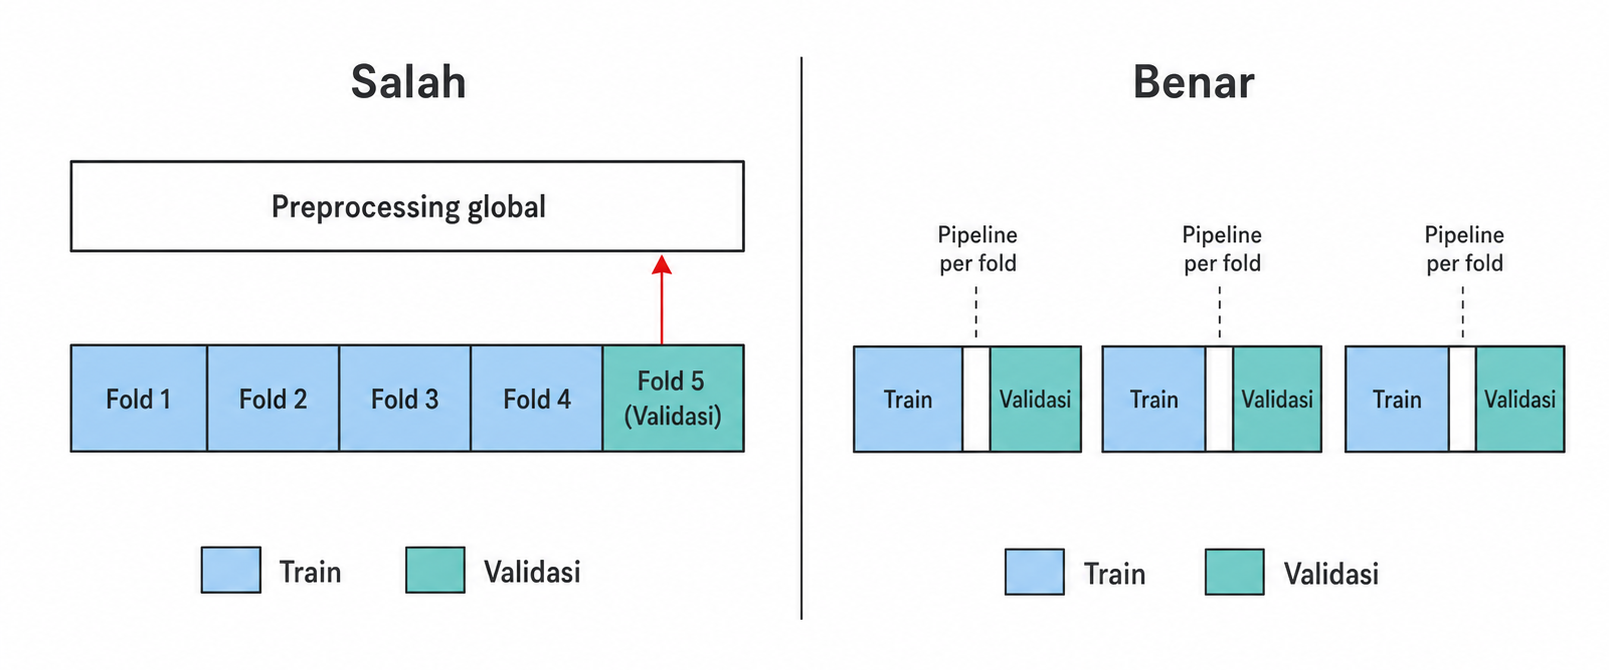
\includegraphics[width=\linewidth,height=0.72\textheight,keepaspectratio]{ch02-fig-4}
\caption{Mekanisme Data Leakage Akibat Transformasi Agregasi Sebelum Pemisahan Dataset}
\label{fig:ch02-fig-4}
\end{figure}

Kerentanan operasi fitur terhadap kontaminasi inilah yang menjadi pemicu perlunya praktik \emph{pipeline} yang benar. Mengisolasi partisi evaluasi secara konsisten tidak dapat digantungkan pada kehati-hatian penulisan skrip manual, melainkan harus dikunci melalui instrumen pemrograman yang terstruktur. Isolasi ini pertama-tama dapat dilakukan di tingkat pustaka menggunakan kelas pembungkus seperti \passthrough{\lstinline!ColumnTransformer!} yang dijahit di dalam objek utama \passthrough{\lstinline!Pipeline!}. Dalam eksekusi validasi (\emph{cross-validation}), struktur ini menjamin bahwa seluruh perhitungan varians atau proporsi dipaksa untuk \emph{fit} ulang pada setiap sub-partisi latih, sehingga membiarkan partisi evaluasinya benar-benar buta dari parameter kalkulasi. Selanjutnya, isolasi juga diterapkan di tingkat infrastruktur. Pada arsitektur produksi, fitur-fitur kompleks disajikan melalui perantara \emph{feature store} seperti Feast. Komponen infrastruktur ini memberlakukan operasi \emph{point-in-time join} yang mengamankan konsistensi waktu; algoritma hanya diizinkan mengakses fitur agregat yang telah divalidasi dan tercatat kuat sebelum stempel kedatangan \emph{event} data prediksi.

\section{Strategi Pemisahan Data yang Benar}\label{strategi-pemisahan-data-yang-benar}

Pemisahan data berfungsi sebagai mekanisme karantina untuk mencegah \emph{leakage} sebelum kita mengeksekusi rekayasa fitur. Memilih strategi pemisahan yang keliru akan menghasilkan evaluasi model yang menyesatkan. Strategi yang tepat sangat bergantung pada struktur asal data dan kemandirian antar-unit observasi.

Terdapat tiga pendekatan utama dalam memisahkan data pelatihan dan pengujian. Pendekatan pertama adalah \emph{random split}, yang memisahkan baris observasi secara acak. Metode ini valid ketika setiap titik observasi bersifat mandiri, karena pengacakan akan mendistribusikan pola secara merata antara kelompok latih dan uji. Namun, pendekatan ini akan memicu \emph{leakage} jika data memiliki struktur kelompok atau runtunan waktu. Pendekatan kedua adalah \emph{group split}, yakni memisahkan observasi berdasarkan identitas subjek. Pendekatan ini wajib diterapkan pada data yang memuat rekam jejak subjek yang sama berulang kali, misalnya pindaian rontgen dari pasien yang sama atau riwayat kunjungan pelanggan. Pendekatan ketiga adalah \emph{temporal split}, yang memisahkan data berdasarkan urutan waktu kronologis untuk memastikan model hanya belajar dari peristiwa masa lalu demi memprediksi masa depan.

\begin{figure}[htbp]\centering
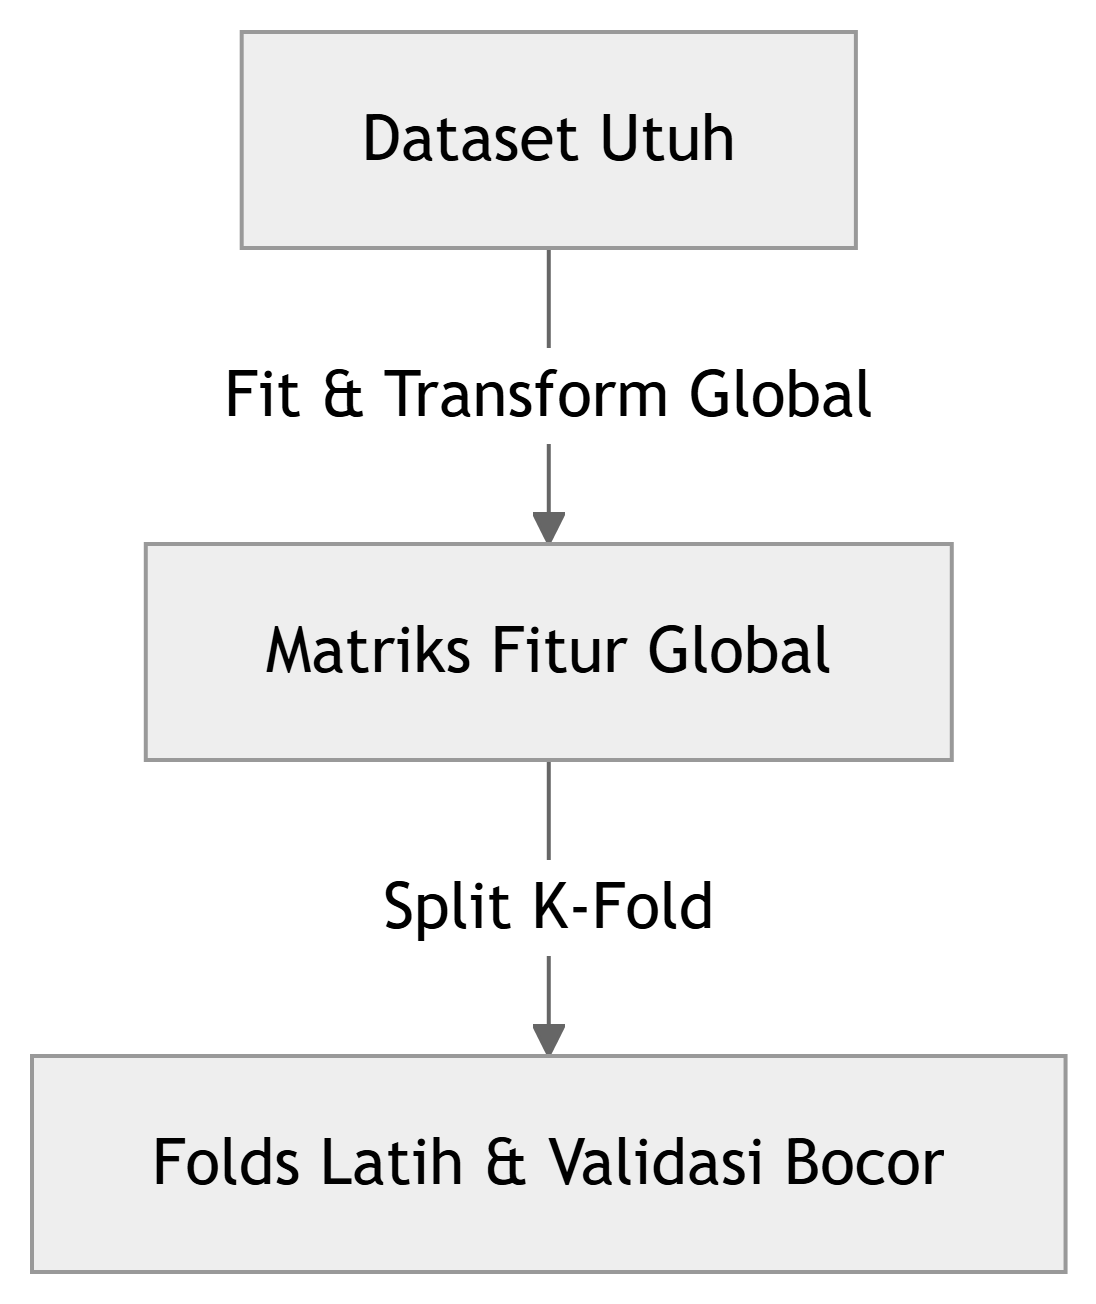
\includegraphics[width=\linewidth,height=0.72\textheight,keepaspectratio]{ch02-fig-5}
\caption{Perbandingan Strategi Pemisahan Data: Random, Group, dan Temporal Split}
\label{fig:ch02-fig-5}
\end{figure}

\textbf{Pemisahan Berbasis Kelompok (Group Split)}
Apabila memaksakan pemisahan acak pada data rekam medis, sebagian rontgen milik pasien A dapat masuk ke kelompok latih, sementara sisa rontgen miliknya jatuh ke kelompok uji. Model cenderung menghafal karakteristik anatomi spesifik pasien tersebut ketimbang belajar membedakan pola penyakit. \emph{Group split} menggeser unit pemisahan dari level baris ke level subjek. Syarat mutlak dari pemisahan ini dirumuskan sebagai \(G_{latih} \cap G_{uji} = \emptyset\), di mana \(G_{latih}\) adalah himpunan pengenal unik subjek (seperti ID pasien) pada partisi pelatihan, dan \(G_{uji}\) adalah himpunan pengenal pada partisi pengujian. Implementasi seperti \passthrough{\lstinline!GroupKFold!} atau \passthrough{\lstinline!StratifiedGroupKFold!} di pustaka \emph{machine learning} memastikan seluruh rekam jejak milik satu subjek masuk secara utuh ke dalam satu partisi, sekaligus mempertahankan distribusi target prediksi.

\textbf{Pemisahan Temporal (Temporal Split)}
Sistem yang beroperasi di dunia nyata tidak memiliki akses ke data masa depan. \emph{Temporal split} menyimulasikan batasan ini melalui titik potong waktu yang tegas. Pada proses \emph{cross-validation} untuk data sekuensial, kelas utilitas seperti \passthrough{\lstinline!TimeSeriesSplit!} memastikan partisi pelatihan selalu berasal dari periode sebelum partisi pengujian. Kita juga dapat mendefinisikan parameter \emph{gap} untuk memberikan jeda observasi antara partisi latih dan uji, yang berguna untuk menyimulasikan latensi ketersediaan fitur saat model diterapkan di lingkungan produksi.

\textbf{Validasi Silang Bersarang (Nested Cross-Validation)}
Bentuk \emph{leakage} lain terjadi ketika kita menala hiperparameter (misalnya ambang batas seleksi fitur) lalu mengevaluasi performa akhir pada partisi data yang sama. Praktik ini memicu bias optimistis karena keputusan penalaan dipengaruhi oleh partisi uji. \emph{Nested cross-validation} menyelesaikan masalah ini dengan menyekat dua proses secara hierarkis: putaran dalam (\emph{inner loop}) digunakan murni untuk menala dan mencari hiperparameter terbaik, sedangkan putaran luar (\emph{outer loop}) digunakan khusus untuk mengestimasi performa generalisasi pada sisa data yang sama sekali tidak tersentuh oleh putaran dalam.

Disiplin pemisahan data ini menjamin bahwa seluruh transformasi fitur selanjutnya dikalibrasi pada partisi yang bersih, sehingga estimasi performa model tetap jujur.

\section{\texorpdfstring{\emph{Pipeline} di Dalam \emph{Cross-Validation}}{Pipeline di Dalam Cross-Validation}}\label{pipeline-di-dalam-cross-validation}

Menguji model dengan satu kali pemisahan data latih dan uji rentan menghasilkan estimasi kinerja yang tidak stabil. Skor akurasi tinggi bisa saja muncul akibat distribusi acak pada satu pemisahan tertentu. Praktisi menggunakan \emph{cross-validation} (validasi silang) untuk mengevaluasi kinerja secara iteratif dan mendapatkan taksiran yang lebih andal.

Secara matematis, estimasi kesalahan melalui \(K\)-Fold \emph{Cross-Validation} dihitung sebagai rata-rata dari seluruh iterasi dengan formula \(CV_{(K)} = \frac{1}{K} \sum_{k=1}^K E_k\). Dalam hal ini, \(K\) adalah total jumlah partisi data (\emph{fold}), dan \(E_k\) mewakili nilai kesalahan (seperti \emph{Mean Squared Error}) saat mengevaluasi model pada \emph{fold} validasi ke-\(k\).

Skema ini membagi himpunan data menjadi kumpulan \emph{fold} berukuran seimbang. Di setiap perputaran, satu \emph{fold} bertindak sebagai blok validasi, dan kumpulan \emph{fold} sisanya disatukan sebagai data pelatihan. Masalah muncul ketika tahapan rekayasa fitur diimplementasikan keliru bersamaan dengan rotasi iteratif ini.

\textbf{Risiko Kebocoran Data dalam Validasi Silang}

Kesalahan paling umum adalah menjalankan fungsi transformasi pada seluruh dataset sebelum fungsi \emph{cross-validation} dipanggil. Jika perhitungan parameter standardisasi dilakukan secara global di awal, nilai statistik tersebut ikut menyerap informasi dari baris-baris data yang nantinya bertindak sebagai blok validasi. Dampaknya terhadap evaluasi metrik sangat menipu: skor validasi akan melonjak tinggi karena distribusi data validasi sudah terdeteksi di tahap pelatihan. Model sebenarnya mempelajari pola observasi yang seharusnya tertutup rapat, sehingga pada akhirnya performa model akan anjlok drastis ketika dihadapkan pada data baru di lingkungan produksi.

\begin{figure}[htbp]\centering
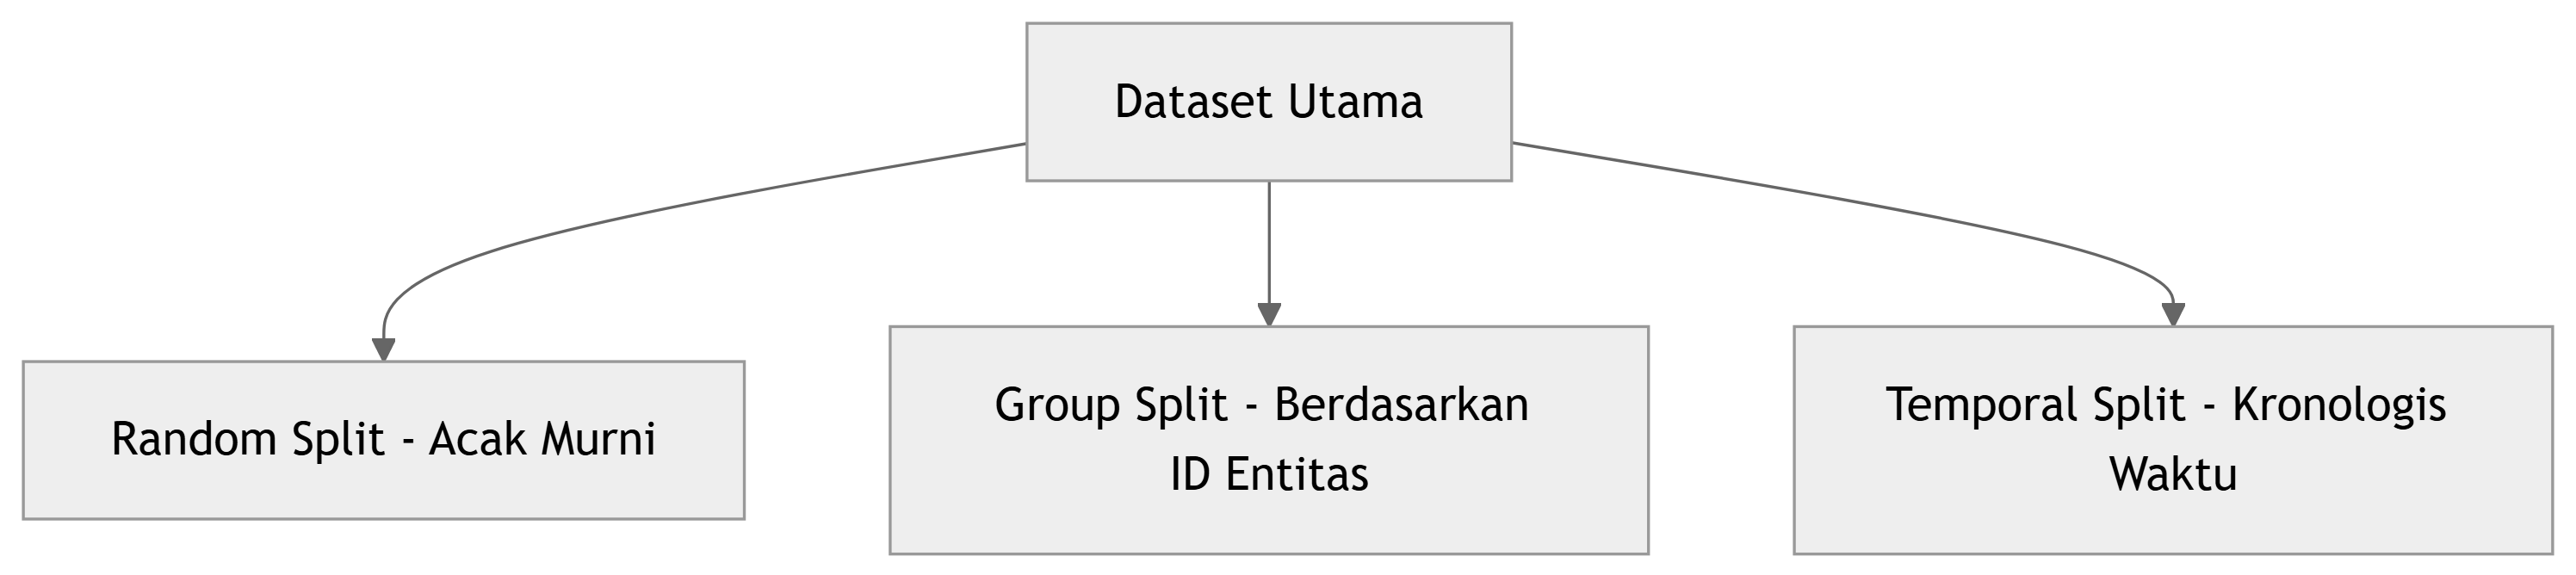
\includegraphics[width=\linewidth,height=0.72\textheight,keepaspectratio]{ch02-fig-6}
\caption{Aliran Data Cross-Validation yang Salah (Bocor)}
\label{fig:ch02-fig-6}
\end{figure}

\begin{figure}[htbp]\centering
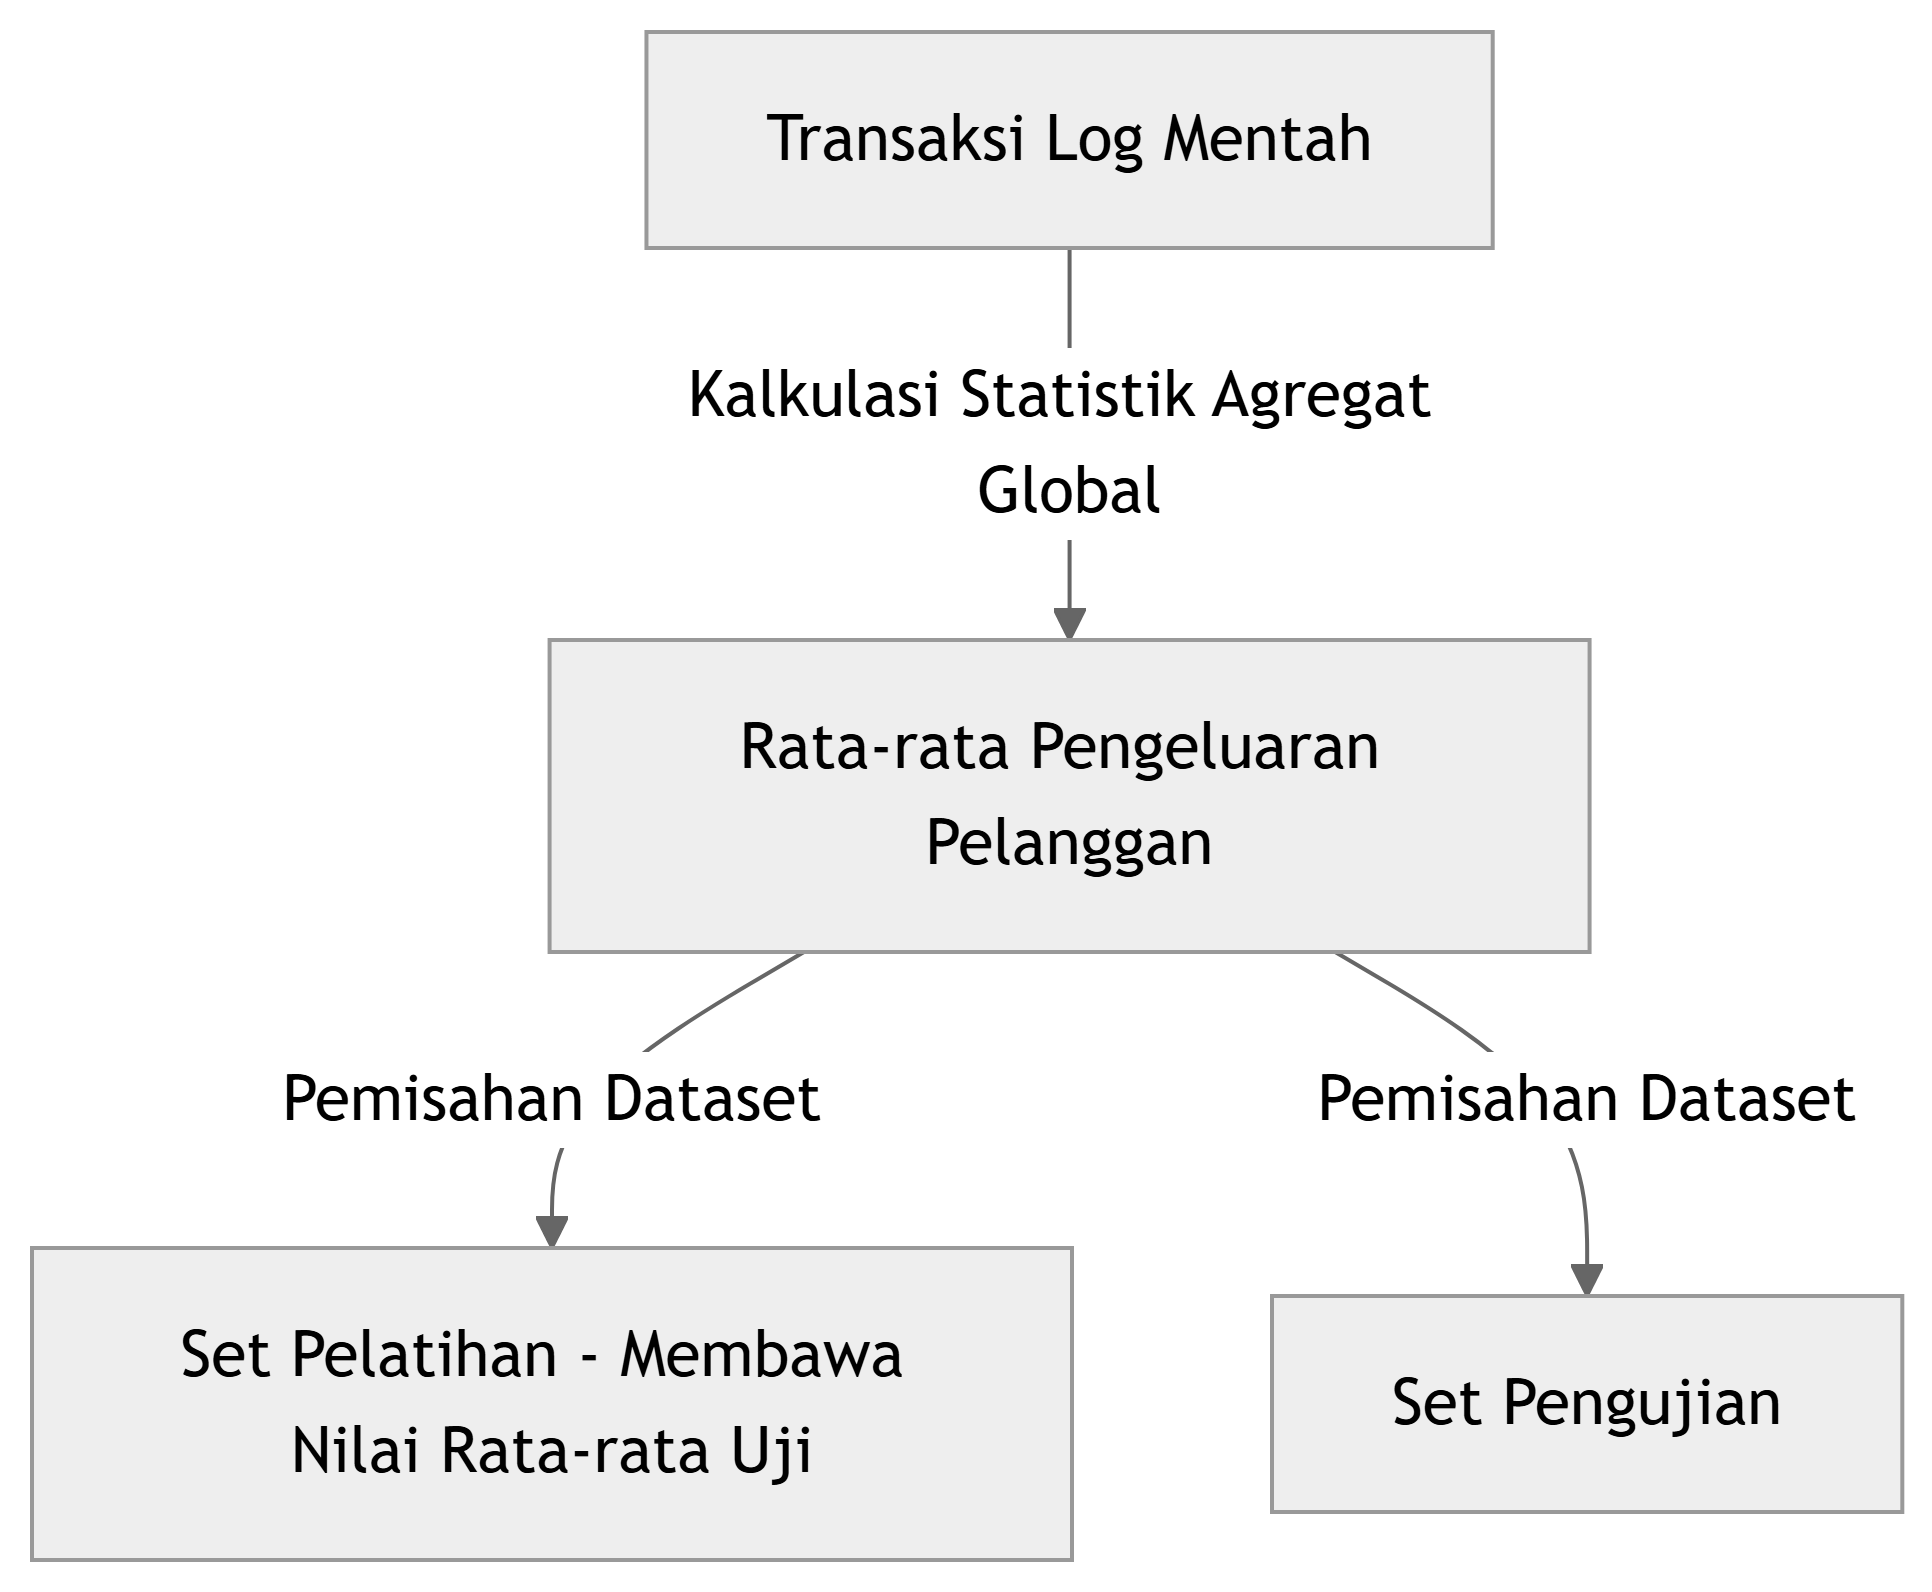
\includegraphics[width=\linewidth,height=0.72\textheight,keepaspectratio]{ch02-fig-7}
\caption{Aliran Data Cross-Validation yang Benar (Terisolasi)}
\label{fig:ch02-fig-7}
\end{figure}

\textbf{Mekanisme Isolasi Transformasi}

Untuk menjamin evaluasi tidak bias, seluruh urutan penyesuaian fitur harus dirangkai ke dalam satu objek \emph{pipeline}. Tabel observasi asli diteruskan beriringan dengan objek \emph{pipeline} ke dalam fungsi silang. Metode ini mengunci ruang eksekusi transformasi berada di dalam perputaran internal setiap tahapan \emph{cross-validation}.

Cara kerja \emph{pipeline} di setiap rotasi silang terbagi menjadi tiga langkah terisolasi. Pertama, tahap penghitungan parameter (\passthrough{\lstinline!fit()!}) pada \emph{pipeline} dibatasi secara ketat hanya pada blok data pelatihan iterasi yang sedang berjalan. Kedua, objek \emph{pipeline} yang sudah menyimpan parameter dari data pelatihan meluncurkan modifikasi data (\passthrough{\lstinline!transform()!}) secara mandiri pada blok validasi yang sedang disisihkan. Ketiga, pada transisi rotasi berikutnya, ukuran acuan seperti nilai tengah imputasi atau simpangan baku akan dibuang dan dihitung ulang dari nol berdasarkan himpunan pelatihan iterasi yang baru.

\textbf{Optimalisasi Komputasi dan Nested CV}

Menjalankan rekayasa fitur berulang kali di dalam skema silang, terlebih bila digabung dengan pencarian \emph{hyperparameter} (\emph{GridSearchCV}), memakan beban komputasi yang masif. Pustaka \emph{machine learning} modern menyediakan dua fasilitas utama untuk mengoptimalkan kendala teknis ini. Fasilitas pertama adalah \emph{caching} transformasi, di mana objek \passthrough{\lstinline!Pipeline!} mendukung argumen \passthrough{\lstinline!memory!} untuk merekam status keluaran langkah \emph{transformer} ke dalam penyimpanan diska. \emph{Pipeline} otomatis akan memanggil hasil kalkulasi yang tersimpan jika parameter dan observasi masukan tidak berubah di perputaran selanjutnya. Fasilitas kedua adalah pendekatan \emph{nested cross-validation}. Untuk mencegah kebocoran informasi melalui pemilihan \emph{hyperparameter}, evaluasi model terbaik dilakukan lewat validasi silang bersarang, di mana perputaran dalam berfokus menala setelan rekayasa fitur, sementara perputaran luar bekerja menaksir kinerja generalisasi murni tanpa intervensi penyetelan algoritma.

\begin{lstlisting}[language=Python]
import tempfile
from shutil import rmtree
from sklearn.model_selection import cross_val_score
from sklearn.pipeline import Pipeline
from sklearn.preprocessing import StandardScaler
from sklearn.impute import SimpleImputer
from sklearn.linear_model import LogisticRegression
from sklearn.datasets import make_classification

# 1. Inisialisasi data dummy untuk simulasi klasifikasi
X, y = make_classification(n_samples=1000, n_features=20, random_state=42)

# 2. Membuat direktori temporer khusus untuk menyimpan cache pipeline
cachedir = tempfile.mkdtemp()

# 3. Mendefinisikan tahapan transformasi dan estimator dalam pipeline
pipeline_steps = [
    ('imputer', SimpleImputer(strategy='median')),
    ('scaler', StandardScaler()),
    ('classifier', LogisticRegression(random_state=42))
]

# 4. Konstruksi pipeline terisolasi dengan parameter cache 'memory'
pipeline = Pipeline(steps=pipeline_steps, memory=cachedir)

# 5. Evaluasi performa model menggunakan skema Cross-Validation (K-Fold = 5)
# Transformasi data terjadi secara aman di dalam putaran internal CV tanpa kebocoran data
scores = cross_val_score(pipeline, X, y, cv=5, scoring='accuracy')

# 6. Bersihkan direktori penyimpanan cache secara aman untuk membebaskan ruang memori
rmtree(cachedir)

print(f"Skor Cross-Validation per lipat: {scores}")
print(f"Rata-rata Akurasi Model: {scores.mean():.4f}")
\end{lstlisting}

\section{Kesalahan Praktik pada Alur Transformasi}\label{kesalahan-praktik-pada-alur-transformasi}

Memahami konsep rekayasa fitur belum tentu menjamin penulisan kode yang bebas masalah. Saat merancang alur transformasi, pengembang sering kali secara tak sengaja melanggar \emph{praktik pipeline yang benar}. Pelanggaran ini merusak integritas model secara diam-diam melalui kebocoran informasi (\emph{data leakage}) atau diskrepansi tipe data. Dokumentasi panduan \emph{Common Pitfalls} dari pustaka \emph{Scikit-Learn} menyoroti beberapa pola kelalaian yang secara konsisten berulang dalam implementasi lapangan.

Pola kelalaian pertama adalah pemanggilan \passthrough{\lstinline!fit_transform!} berulang pada himpunan uji. Metode \passthrough{\lstinline!fit_transform!} didesain untuk menghitung konstanta acuan (seperti \emph{mean} dan varians) sekaligus menerapkannya pada himpunan data latih. Kesalahan fatal terjadi ketika perintah ini dipanggil kembali pada himpunan uji (\emph{test set}). Pemanggilan ulang ini akan menimpa parameter acuan latih, lalu menggantinya dengan rentang skala yang murni bersandar pada distribusi himpunan uji, sehingga kontrak konsistensi pun hancur. Secara matematis, transformasi \emph{Z-score} pada data uji harus selalu tunduk pada parameter data latih melalui persamaan \(x'_{\text{test}} = \frac{x_{\text{test}} - \mu_{\text{train}}}{\sigma_{\text{train}}}\). Dalam persamaan ini, \(\mu_{\text{train}}\) dan \(\sigma_{\text{train}}\) secara eksklusif ditarik dari perhitungan tahap \passthrough{\lstinline!fit!} pada data latih. Kelalaian ini terbukti dapat mengakibatkan lonjakan galat prediksi secara ekstrem. Aturan mutlaknya adalah himpunan uji hanya boleh dieksekusi menggunakan perintah \passthrough{\lstinline!transform!}.

Pola kelalaian kedua adalah seleksi fitur sebelum pemisahan data, sebuah bentuk kebocoran data yang paling sering tidak disadari. Praktisi kerap menyeleksi dan membuang fitur menggunakan seluruh tumpukan data utuh sebelum membaginya menjadi himpunan latih dan uji. Membiarkan mekanisme seleksi mengintip sebaran target dari data uji akan melahirkan ilusi performa yang sangat meyakinkan, bahkan bisa menggelembungkan akurasi model pada tumpukan \emph{noise} acak secara artifisial.

Pola kelalaian ketiga adalah ekstraksi \emph{embedding} global. Bentuk modern dari kontaminasi silang ini muncul pada pemrosesan teks, di mana praktisi menginisiasi vektorisasi (seperti matriks TF-IDF) terhadap gabungan korpus dokumen utuh, kemudian baru membelah hasilnya. Praktik ini secara langsung membocorkan informasi frekuensi kemunculan kata spesifik dari himpunan uji ke dalam fitur latih. Seluruh proses inisialisasi kamus kosakata mutlak wajib diletakkan setelah partisi selesai.

\begin{figure}[htbp]\centering
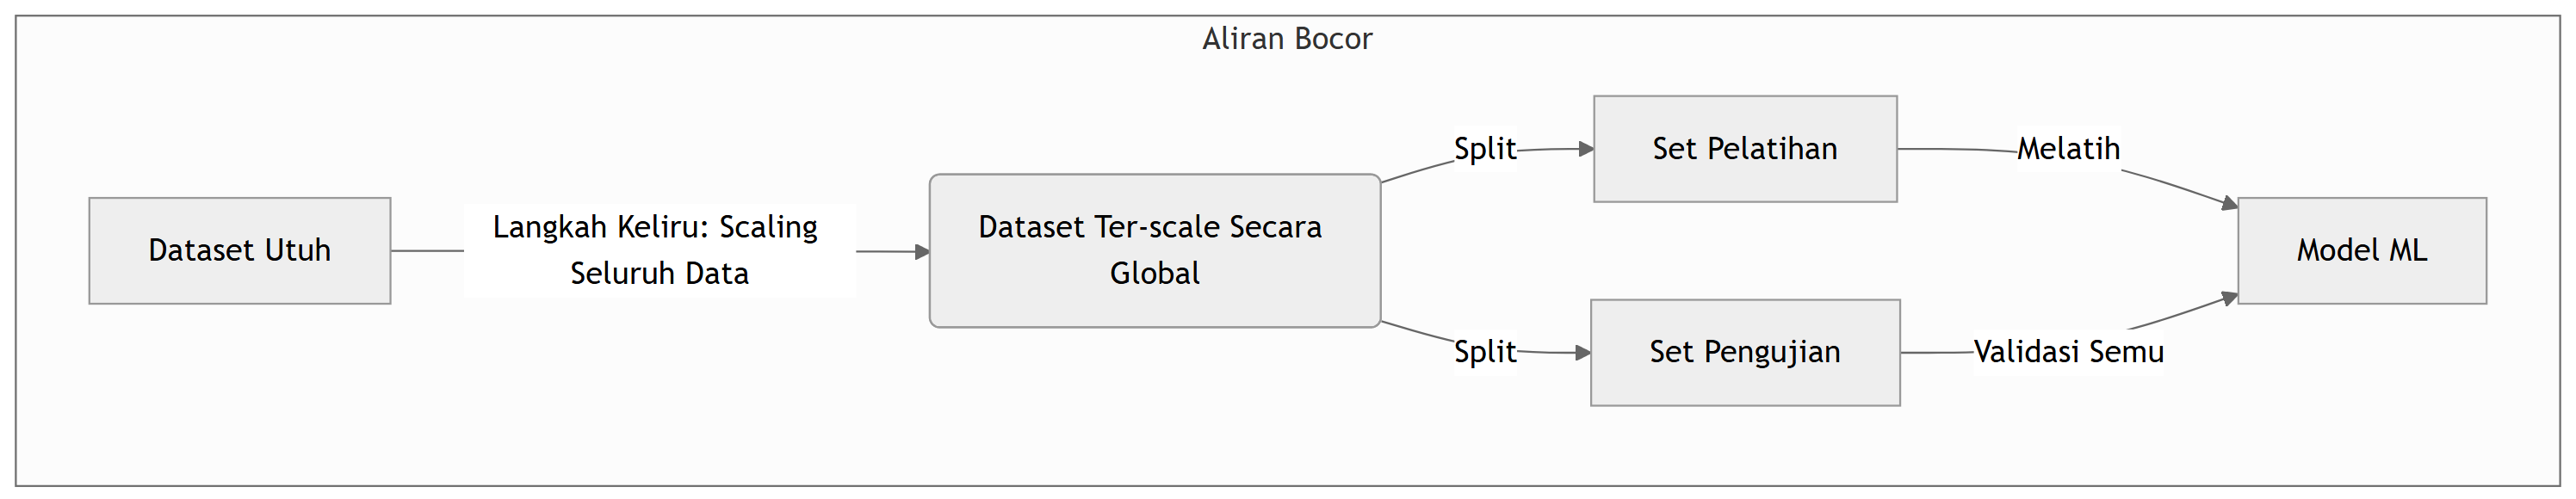
\includegraphics[width=\linewidth,height=0.72\textheight,keepaspectratio]{ch02-fig-8}
\caption{Aliran Data Imputasi Global yang Salah (Bocor)}
\label{fig:ch02-fig-8}
\end{figure}

\begin{figure}[htbp]\centering
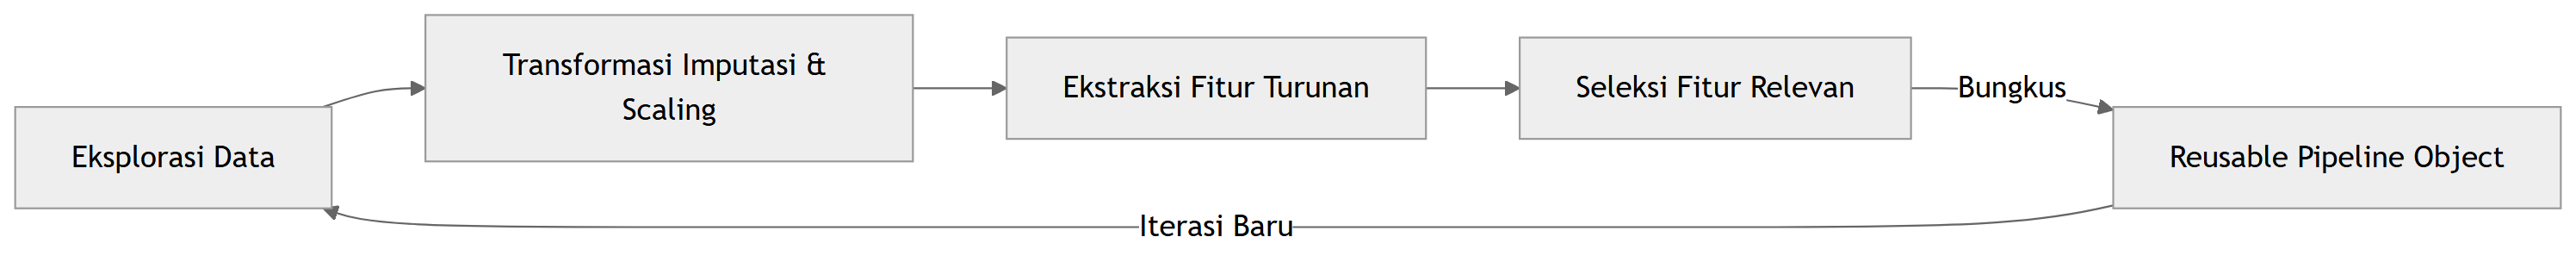
\includegraphics[width=\linewidth,height=0.72\textheight,keepaspectratio]{ch02-fig-9}
\caption{Aliran Data Imputasi dengan Pipeline Tertutup yang Benar}
\label{fig:ch02-fig-9}
\end{figure}

Pola kelalaian terakhir adalah manipulasi fitur kustom di luar objek \emph{pipeline}. Mengubah format matriks menggunakan fungsi modifikasi lepas (seperti penghapusan spasi teks di luar kerangka \emph{estimator}) sangatlah rapuh. Ketika sistem berpindah ke lingkungan produksi, sekuens modifikasi tanpa pembungkus ini hampir pasti terlupakan. Solusi permanennya adalah membungkus logika tersebut ke dalam kelas pewaris (\emph{custom transformer}), sehingga ia dapat disatukan dan diekspor (\emph{serialize}) di dalam satu \emph{pipeline} yang tak terpisahkan.

\section{\texorpdfstring{Studi Kasus: \emph{Pipeline} yang Valid vs.~\emph{Pipeline} yang Bocor}{Studi Kasus: Pipeline yang Valid vs.~Pipeline yang Bocor}}\label{studi-kasus-pipeline-yang-valid-vs.-pipeline-yang-bocor}

Dalam skenario pembuatan model penaksir harga \emph{real estate}, sebagian data pada atribut ukuran lahan mungkin kosong. Nilai yang hilang ini dapat diisi menggunakan metode imputasi rata-rata. Urutan eksekusi imputasi menentukan apakah evaluasi model berjalan objektif atau mengalami kebocoran data (\emph{data leakage}). Berikut adalah perbandingan dua pendekatan komputasi untuk menangani kondisi tersebut.

Pendekatan pertama adalah manipulasi global yang menghasilkan kebocoran data. Pada praktik keliru ini, seluruh baris \emph{dataset} utuh digunakan untuk menghitung nilai rata-rata ukuran lahan sebelum pemisahan data dilakukan. Sel kosong pada seluruh observasi kemudian diisi dengan nilai rata-rata global tersebut, baru setelahnya data dipisah menjadi himpunan pelatihan dan pengujian. Dampak dari urutan terbalik ini sangat jelas: nilai imputasi pada data latih secara tak langsung ikut dibentuk oleh statistik data uji. Akurasi evaluasi akan melonjak secara semu karena model telah terekspos pada karakteristik distribusi data uji sejak tahap pembentukan fitur.

Pendekatan kedua adalah isolasi melalui \emph{pipeline}, yakni pendekatan yang sah dan tervalidasi. Langkah paling awal yang wajib dilakukan adalah memotong \emph{dataset} menjadi himpunan pelatihan murni dan himpunan pengujian independen. Setelah dipotong, nilai rata-rata ukuran lahan dihitung murni menggunakan observasi yang ada pada himpunan pelatihan. Nilai rata-rata ini kemudian diterapkan untuk mengisi sel kosong di fase pelatihan, dan kelak parameter rata-rata yang sama persis digunakan secara konsisten pada tahap pengujian.

Secara matematis, jika \(N_{train}\) adalah jumlah observasi valid pada data latih, rata-rata \(\mu_{train}\) dihitung sebagai:

\[ \mu_{train} = \frac{1}{N_{train}} \sum_{i=1}^{N_{train}} x_i \]

Pada persamaan tersebut, \(x_i\) mewakili nilai ukuran lahan yang tersedia di dalam data latih. Nilai \(\mu_{train}\) tunggal ini kemudian dipertahankan untuk menambal nilai kosong pada observasi di data uji. Pendekatan ini memastikan data uji tetap terisolasi dan tidak berkontribusi pada komputasi parameter fitur.

Saat dievaluasi, performa dari pendekatan kedua umumnya lebih rendah dibandingkan pendekatan pertama. Skor yang menurun ini justru mencerminkan kemampuan prediksi yang realistis saat model menghadapi observasi baru. Tanpa isolasi \emph{pipeline} yang tegas, rekayasa fitur berisiko meloloskan kalkulasi cacat yang membuat validasi model tidak sah. Pada skala produksi, pencegahan kebocoran temporal ini juga dapat diamankan oleh infrastruktur pelengkap seperti \emph{feature store} melalui mekanisme \emph{point-in-time join}, sehingga data dari masa depan terblokir dan tidak memengaruhi perhitungan fitur pelatihan historis.

\section{Sintesis Keputusan dan Prinsip Akhir}\label{sintesis-keputusan-dan-prinsip-akhir}

Keamanan dan konsistensi naskah data sebelum diumpankan ke dalam model ditentukan oleh kedisiplinan kita dalam menerapkan prinsip isolasi data.

\textbf{Panduan Praktis Pencegahan Kebocoran.} Seluruh parameter prapemrosesan (seperti nilai rata-rata imputer, batas kuantil scaling, atau pemetaan kategori) wajib dipelajari (\emph{fit}) murni dari himpunan data latih. Data uji atau data validasi harus diperlakukan sebagai entitas steril yang hanya boleh dimodifikasi lewat operasi \emph{transform} searah tanpa menyumbang nilai statistik apa pun.

\textbf{Pilihan Strategi Pemisahan.} Pemisahan data harus disesuaikan dengan struktur asli informasi. Gunakan \emph{random split} hanya jika setiap observasi bersifat mandiri dan terdistribusi seragam. Jika data memiliki dependensi waktu, terapkan \emph{temporal split} untuk mencegah model mengintip masa depan. Untuk data yang menyimpan beberapa pengamatan berulang dari subjek yang sama, wajib menggunakan \emph{group split} agar karakteristik subjek tidak bocor melintasi batas partisi.

\textbf{Evaluasi dan Validasi.} Setiap keputusan seleksi atau penalaan parameter fitur harus dikurung di dalam skema \emph{cross-validation} yang ketat. Menggunakan model hibrida atau model berbasis pohon tidak membebaskan kita dari keharusan merancang \emph{pipeline} tertutup. Keberhasilan validasi offline yang jujur adalah satu-satunya jaminan bahwa model akan memberikan performa yang konsisten saat melayani prediksi di produksi.

Kode sumber lengkap dan demonstrasi visual bagaimana membandingkan pipeline yang valid dan yang bocor pada skema evaluasi dapat diuji langsung melalui materi di repositori pendamping buku ini.

% ==========================================================================
% ch03.tex — dihasilkan otomatis dari website/chapters/ch03.qmd
% Boleh disunting manual. 'sync' hanya menimpa bila .qmd berubah DAN .tex
% belum disunting; kalau keduanya berubah, dilewati (pakai --force).
% qmd-sha1: 6fb2b7c80160
% tex-sha1: 6ca1163ce2d0
% ==========================================================================
% >>>>> ISI OTOMATIS (jangan hapus baris ini) >>>>>
\chapter{Representasi Fitur Numerik}\label{representasi-fitur-numerik}

Fitur numerik adalah bentuk representasi kuantitatif yang paling umum ditemui dalam data tabular. Namun, angka-angka mentah di dunia nyata menyimpan berbagai hambatan komputasi yang dapat mendistorsi proses pemelajaran mesin. Di satu sisi, perbedaan rentang skala antar-atribut yang sangat kontras, misalnya membandingkan variabel pendapatan dalam jutaan dengan variabel usia dalam puluhan, secara otomatis akan membelokkan perhitungan fungsi objektif pada model berbasis jarak spasial atau gradien. Di sisi lain, sebaran data yang menceng ekstrem akibat pencilan (\emph{outlier}) dapat melanggar asumsi dasar statistik yang dibutuhkan oleh algoritma parametrik untuk dapat belajar secara optimal.

Bab ini akan mengupas tuntas cara menata kembali representasi fitur numerik agar sesuai dengan karakteristik matematis algoritma model. Kita mendalami teknik penskalaan standar, penanganan pencilan berbasis kuartil yang tangguh (\emph{robust}), hingga pemampatan distribusi melengkung menggunakan transformasi parametrik dan non-parametrik. Memahami kapan, mengapa, dan bagaimana memodifikasi rentang sebaran angka ini merupakan bekal penting untuk menstabilkan konvergensi model dan mendongkrak ketajaman hasil prediksi.

\section{Skala dan Distribusi: Mengapa Fitur Numerik Butuh Transformasi}\label{skala-dan-distribusi-mengapa-fitur-numerik-butuh-transformasi}

Algoritma \emph{machine learning} menginterpretasikan angka murni berdasarkan besaran matematisnya. Model tidak memiliki pemahaman bawaan mengenai konteks atau satuan ukur dari sebuah nilai. Angka 10.000.000 selalu diproses jauh lebih besar daripada 50, meskipun angka pertama mewakili pendapatan tahunan dan angka kedua mewakili usia manusia. Sifat komputasi yang harfiah ini menimbulkan dua masalah utama saat memproses fitur numerik mentah.

\textbf{Dominasi Skala pada Fungsi Objektif.}\label{dominasi-skala-pada-fungsi-objektif}

Skala merujuk pada rentang nilai observasi dari sebuah variabel. Ketika algoritma menerima fitur-fitur dengan rentang skala yang terlampau jauh berbeda, fitur dengan varians besar akan mendominasi perhitungan objektif.

Masalah ini terlihat jelas pada algoritma berbasis metrik jarak, yang mencari pola kedekatan antar data menggunakan persamaan jarak Euclidean:

\[ d(p, q) = \sqrt{\sum_{i=1}^{n} (p_i - q_i)^2} \]

Di mana \(d(p, q)\) mewakili jarak total antara dua titik observasi \(p\) dan \(q\), sedangkan \(p_i\) dan \(q_i\) adalah nilai numerik dari fitur ke-\(i\).

Bila model mengevaluasi observasi dengan fitur gaji (rentang jutaan rupiah) dan fitur umur (rentang puluhan tahun), kuadrat selisih dari gaji menghasilkan angka yang sangat besar. Angka dominan ini sepenuhnya menutupi selisih nilai umur, sehingga fitur umur menjadi tidak berguna bagi pemetaan algoritma.

Selain itu, pada algoritma berbasis gradien seperti regresi linier dan jaringan saraf tiruan, perbedaan skala antar fitur yang drastis memperlambat perhitungan iteratif. Kondisi ekstrem bahkan mampu menggagalkan model mencapai konvergensi yang stabil, karena arsitektur dasarnya mengasumsikan seluruh fitur beroperasi pada skala yang sebanding.

\textbf{Distribusi Menceng Melanggar Asumsi Model.}\label{distribusi-menceng-melanggar-asumsi-model}

Bentuk persebaran observasi data juga berdampak langsung pada kualitas pemodelan. Data nyata sering membentuk distribusi menceng (\emph{skewed distribution}), yaitu persebaran data yang tidak simetris dan memiliki satu ekor memanjang akibat nilai-nilai ekstrem.

\begin{figure}[htbp]\centering
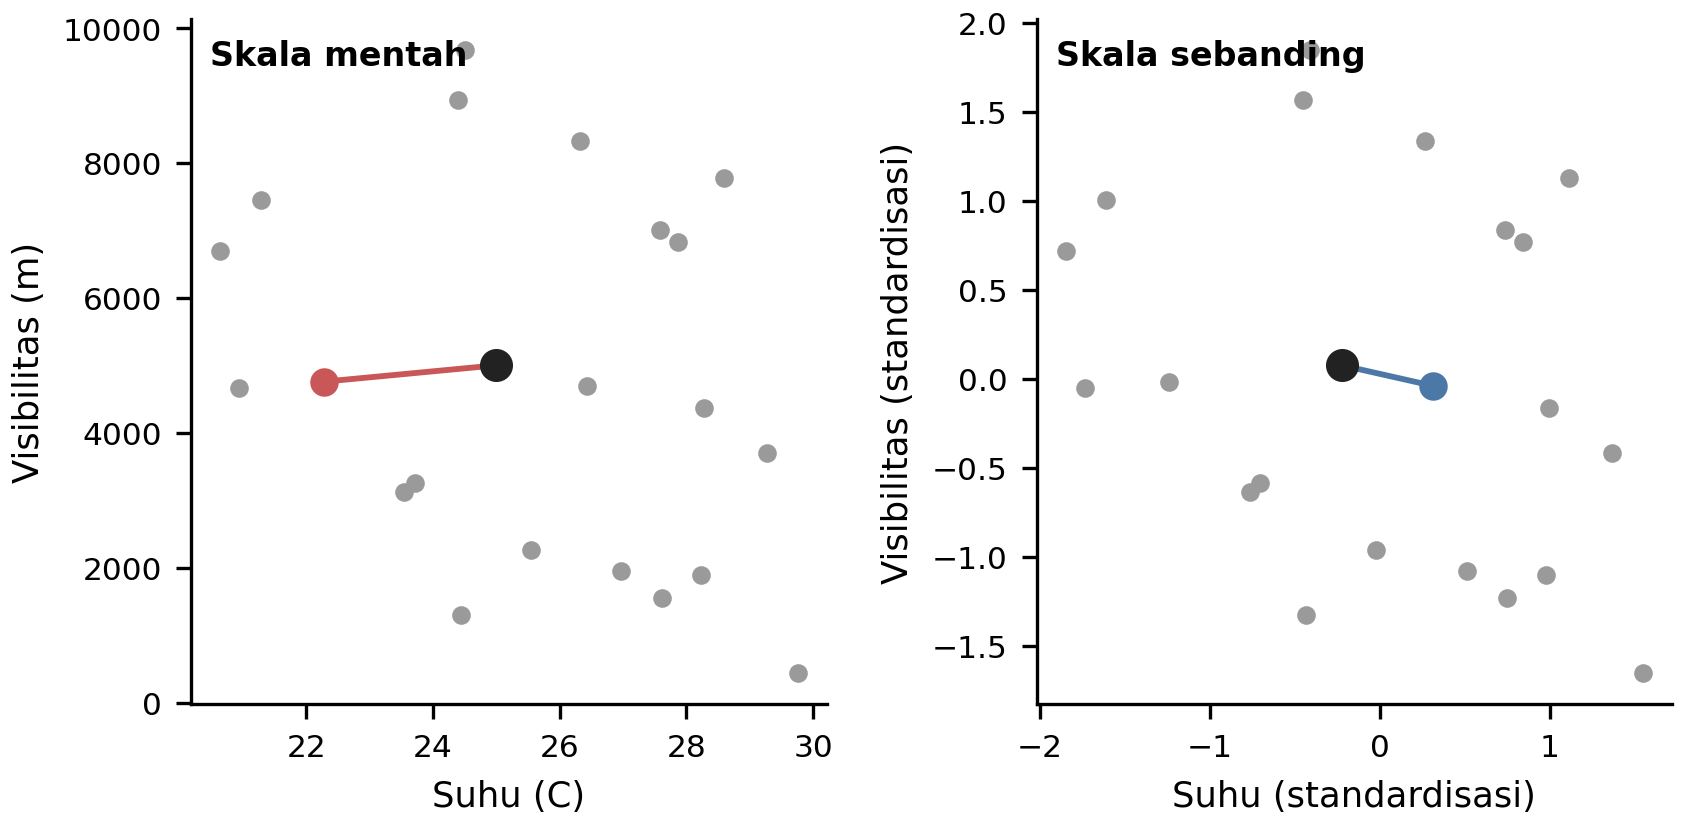
\includegraphics[width=\linewidth,height=0.72\textheight,keepaspectratio]{ch03-fig-1}
\caption{Perbandingan Distribusi Nilai Menggunakan Metode Skala Min-Max dan Standardisasi}
\label{fig:ch03-fig-1}
\end{figure}

Bentuk distribusi yang asimetris menciptakan hambatan komputasi bagi algoritma melalui dua pola utama. Pertama, ia melanggar asumsi sebaran yang dibutuhkan oleh model; mayoritas model linier mengasumsikan distribusi data terpusat stabil di sekitar nilai rata-rata, sehingga data menceng secara langsung akan membelokkan garis regresi. Kedua, algoritma sangat sensitif terhadap galat karena cara kerjanya yang meminimalkan \emph{error} secara agregat. Sekelompok kecil observasi ekstrem di ujung kurva akan menghasilkan kalkulasi galat yang proporsional besar. Akibatnya, model akan menggeser bobot fiturnya secara berlebihan untuk mengakomodasi sebagian kecil observasi ekstrem tersebut, yang pada akhirnya mengorbankan akurasi untuk mayoritas data normal.

Karena besaran angka mentah berbenturan dengan mekanisme komputasi algoritma, fitur numerik wajib ditransformasi. Penyesuaian rentang skala dan perbaikan bentuk distribusi memastikan setiap fitur memiliki kesempatan setara untuk berkontribusi pada hasil prediksi.

\section{Standardisasi dan Skala Min-Max}\label{standardisasi-dan-skala-min-max}

Algoritma pemelajaran mesin berbasis jarak (seperti \emph{k-Nearest Neighbors}) dan turunan gradien (seperti regresi linier) sensitif terhadap skala fitur numerik. Jika model memproses fitur usia dalam skala puluhan dan harga rumah dalam skala jutaan, fitur harga rumah akan mendominasi komputasi akibat magnitudo nominalnya. Penyesuaian skala diperlukan agar seluruh input memiliki kontribusi yang setara. Terdapat dua metode prapemrosesan utama: standardisasi dan skala min-max.

\textbf{Standardisasi.}\label{standardisasi}

Standardisasi memodifikasi sebaran nilai fitur agar memiliki rata-rata nol dengan deviasi baku satu. Proses ini menghitung nilai baku (\emph{Z-score}) dari setiap titik observasi menggunakan persamaan:

\[ z = \frac{x - \mu}{\sigma} \]

Dalam rumus ini, \(z\) adalah nilai hasil standardisasi, \(x\) adalah observasi nilai asli, sedangkan \(\mu\) dan \(\sigma\) berturut-turut merupakan rata-rata dan deviasi baku dari variabel tersebut. Standardisasi memiliki beberapa karakteristik utama. Pertama, metode ini mempertahankan jarak proporsional sehingga rasio komparatif antar-titik data tetap sesuai dengan bentuk sebaran aslinya. Kedua, ia lebih toleran terhadap nilai ekstrem; titik pencilan (\emph{outlier}) tidak dipaksa mengecil dan posisi ekstremnya dipertahankan (misalnya \(z = 4.5\)), memfasilitasi algoritma yang memang membutuhkan informasi abnormal tersebut. Terakhir, rentang nilai akhirnya tidak dibatasi atau dikurung dalam batas minimum dan maksimum yang kaku.

\textbf{Skala Min-Max (\emph{Min-Max Scaling}).}\label{skala-min-max-min-max-scaling}

Skala min-max memampatkan seluruh nilai numerik ke dalam rentang tertutup, umumnya interval nilai \(0\) hingga \(1\). Transformasi ini dihitung menggunakan formula kompresi:

\[ x_{scaled} = \frac{x - x_{min}}{x_{max} - x_{min}} \]

Di mana \(x_{scaled}\) melambangkan nilai setelah diskalakan, \(x\) adalah observasi nilai asli, sementara \(x_{min}\) dan \(x_{max}\) adalah batas observasi terkecil dan terbesar pada fitur tersebut. Karakteristik skala min-max sangat bergantung pada batasan absolut. Metode ini memaksakan rentang yang konstan, di mana nilai terkecil dipetakan secara eksak menjadi \(0\), dan observasi terbesar menjadi \(1\). Konsekuensinya, metode ini sangat sensitif terhadap pencilan. Jika terdapat \emph{outlier} tunggal dengan nilai ekstrem, rentang denominasi (\(x_{max} - x_{min}\)) akan membesar drastis. Akibatnya, kelompok data mayoritas justru terkompresi rapat di kisaran desimal sempit yang mendekati nilai nol.

\begin{figure}[htbp]\centering
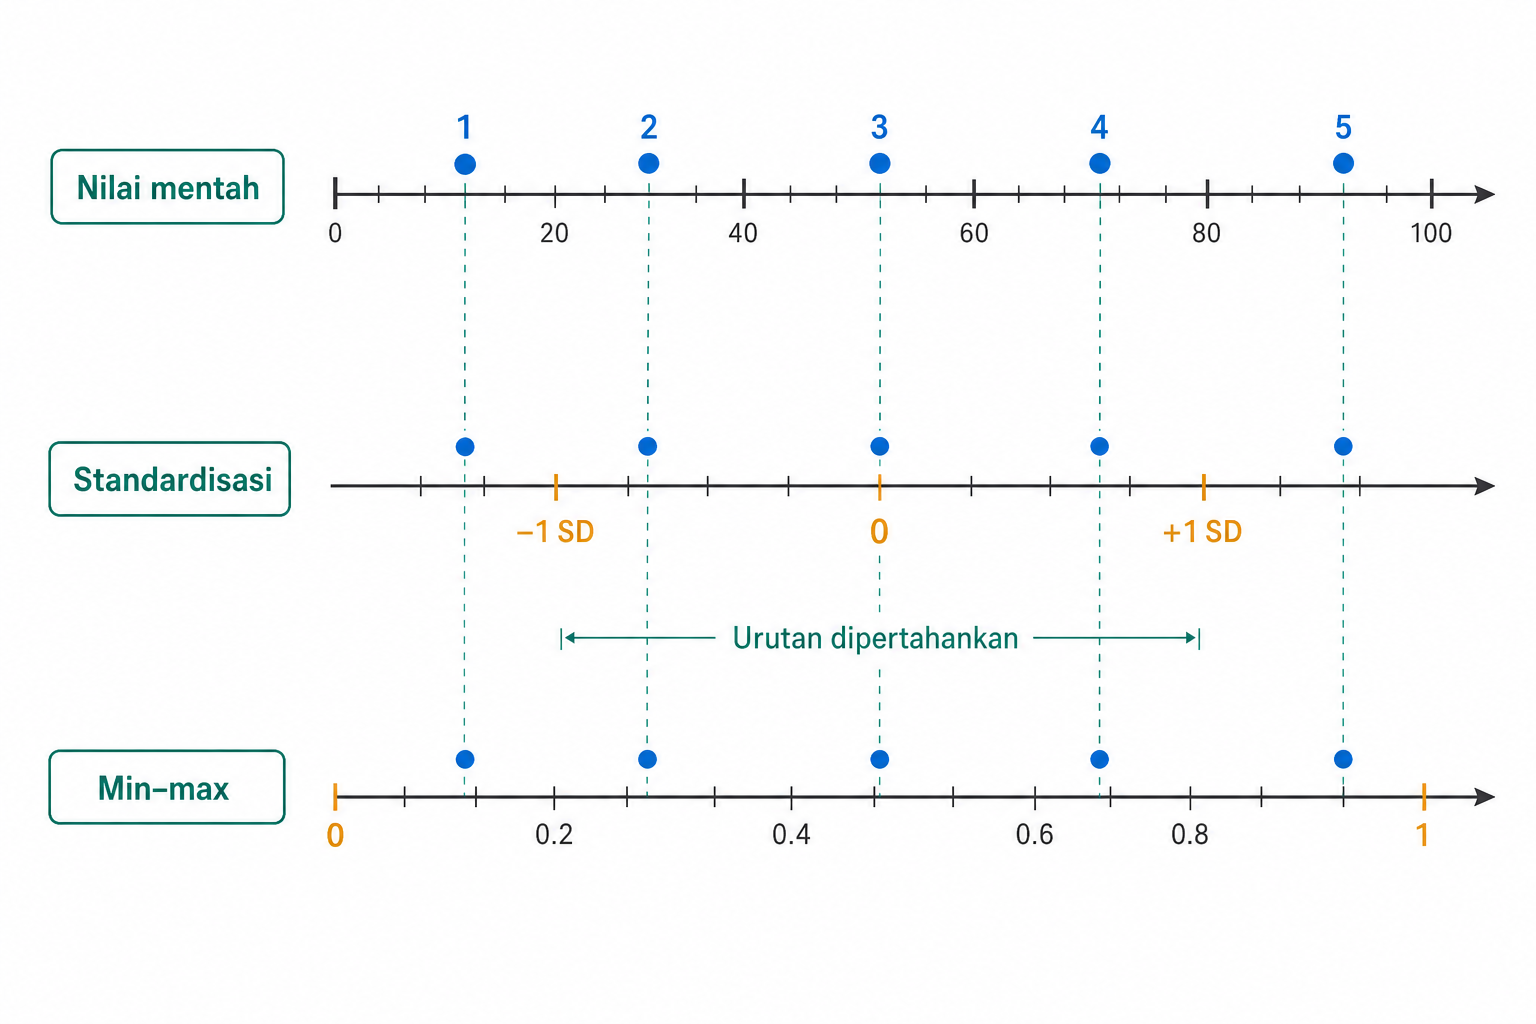
\includegraphics[width=\linewidth,height=0.72\textheight,keepaspectratio]{ch03-fig-2}
\caption{Skema Scaling Menormalkan Rentang Angka Antar Dimensi Fitur}
\label{fig:ch03-fig-2}
\end{figure}

\textbf{Kriteria Penggunaan.}\label{kriteria-penggunaan}

Pemilihan metode penskalaan sangat bergantung pada karakteristik matematis dari algoritma yang akan digunakan. Standardisasi sangat disarankan untuk model linier dan algoritma berbasis jarak Euclidean (seperti \emph{Support Vector Machine} atau \emph{k-Nearest Neighbors}). Pendekatan ini tidak merusak variansi jarak \emph{outlier} dan mampu memuluskan laju konvergensi fungsi objektif. Sebaliknya, skala min-max lebih tepat dipilih untuk algoritma yang memetakan fungsi pada ruang terbatas konstan. Metode ini relevan untuk memproses representasi fisik dengan rentang mutlak (misalnya nilai intensitas piksel 0-255 pada citra digital) atau sebagai asupan awal untuk unit aktivasi tertentu pada jaringan saraf tiruan (\emph{neural network}).

\section{Robust Scaling dan Penanganan Outlier}\label{robust-scaling-dan-penanganan-outlier}

Standardisasi mengandalkan nilai rata-rata dan deviasi standar untuk menyesuaikan skala fitur numerik. Pendekatan ini bekerja dengan baik pada distribusi normal, tetapi memiliki kelemahan: perhitungannya sangat rentan terhadap \emph{outlier} atau nilai ekstrem. Jika sebuah populasi data memiliki anomali yang terlalu tinggi atau rendah, perhitungan rata-rata akan bergeser, dan deviasi standar akan melebar secara semu.

Misalnya pada data pendapatan karyawan di sebuah perusahaan. Mayoritas staf menerima gaji standar, tetapi ada satu orang CEO dengan penghasilan ribuan kali lipat lebih besar. Pendapatan CEO ini menarik nilai rata-rata ke atas secara drastis. Jika kita memaksakan standardisasi pada kondisi ini, gaji karyawan reguler akan tertekan dan saling berhimpit pada area sempit di bagian bawah skala. Variasi asli antar-karyawan biasa menjadi hilang karena tertutup oleh rentang angka yang melebar akibat satu anomali.

Untuk mengatasi masalah ini, kita menggunakan pendekatan \emph{robust scaling}. Metode ini mengganti parameter acuan dengan metrik yang lebih kebal terhadap nilai ekstrem. Pertama, ia menggunakan median untuk menggantikan rata-rata (\(Q_2\)). Median murni melihat posisi urutan sehingga tidak terseret oleh angka ekstrem di ujung distribusi. Kedua, ia menggunakan Rentang Antarkuartil (IQR) untuk menggantikan deviasi standar. IQR mengukur jarak antara persentil ke-25 (\(Q_1\)) dan persentil ke-75 (\(Q_3\)), sehingga metrik ini hanya mengevaluasi sebaran 50 persen data di pusat populasi dan secara alami mengabaikan anomali di kedua ujungnya.

Transformasi \emph{robust scaling} menggunakan formula dasar \(x'_{i} = \frac{x_i - Q_2}{Q_3 - Q_1}\). Di sini, \(x'_{i}\) adalah nilai fitur setelah transformasi, \(x_i\) adalah nilai fitur asli, \(Q_2\) adalah median, dan penyebut \(Q_3 - Q_1\) mewakili IQR. Melalui formula ini, \emph{robust scaling} memastikan titik-titik data normal tetap tersebar secara proporsional. Anomali ekstrem dipertahankan pada posisinya yang jauh dari pusat tanpa merusak skala kelompok data utama.

Selain penyesuaian skala, penanganan \emph{outlier} sering dilakukan melalui pembatasan rentang secara eksplisit, yang dikenal sebagai \emph{clipping} atau \emph{winsorization}. Alih-alih membiarkan anomali memiliki nilai bebas, \emph{winsorization} memotong data dan mengganti angka di luar ambang batas dengan nilai batas maksimum atau minimum tersebut.

Penentuan batas pemotongan (\emph{clipping} atau \emph{winsorization}) dapat dilakukan melalui beberapa metode. Metode pertama adalah batas IQR, di mana titik data yang melebihi \(Q_3 + 1.5 \times \text{IQR}\) atau kurang dari \(Q_1 - 1.5 \times \text{IQR}\) dipotong menjadi batas nilai maksimum atau minimum tersebut. Metode kedua menggunakan batas \emph{Median Absolute Deviation} (MAD), yaitu mengukur deviasi absolut median yang secara statistik terbukti lebih kuat terhadap kontaminasi ekstrem dibandingkan IQR. Pendekatan ini sangat disarankan untuk distribusi dengan kepadatan \emph{outlier} yang tinggi. Metode ketiga adalah batas persentil, yang menetapkan ambang pemotongan kaku berdasarkan persentil tertentu, seperti memotong secara merata semua nilai di bawah persentil ke-1 dan di atas persentil ke-99.

\begin{figure}[htbp]\centering
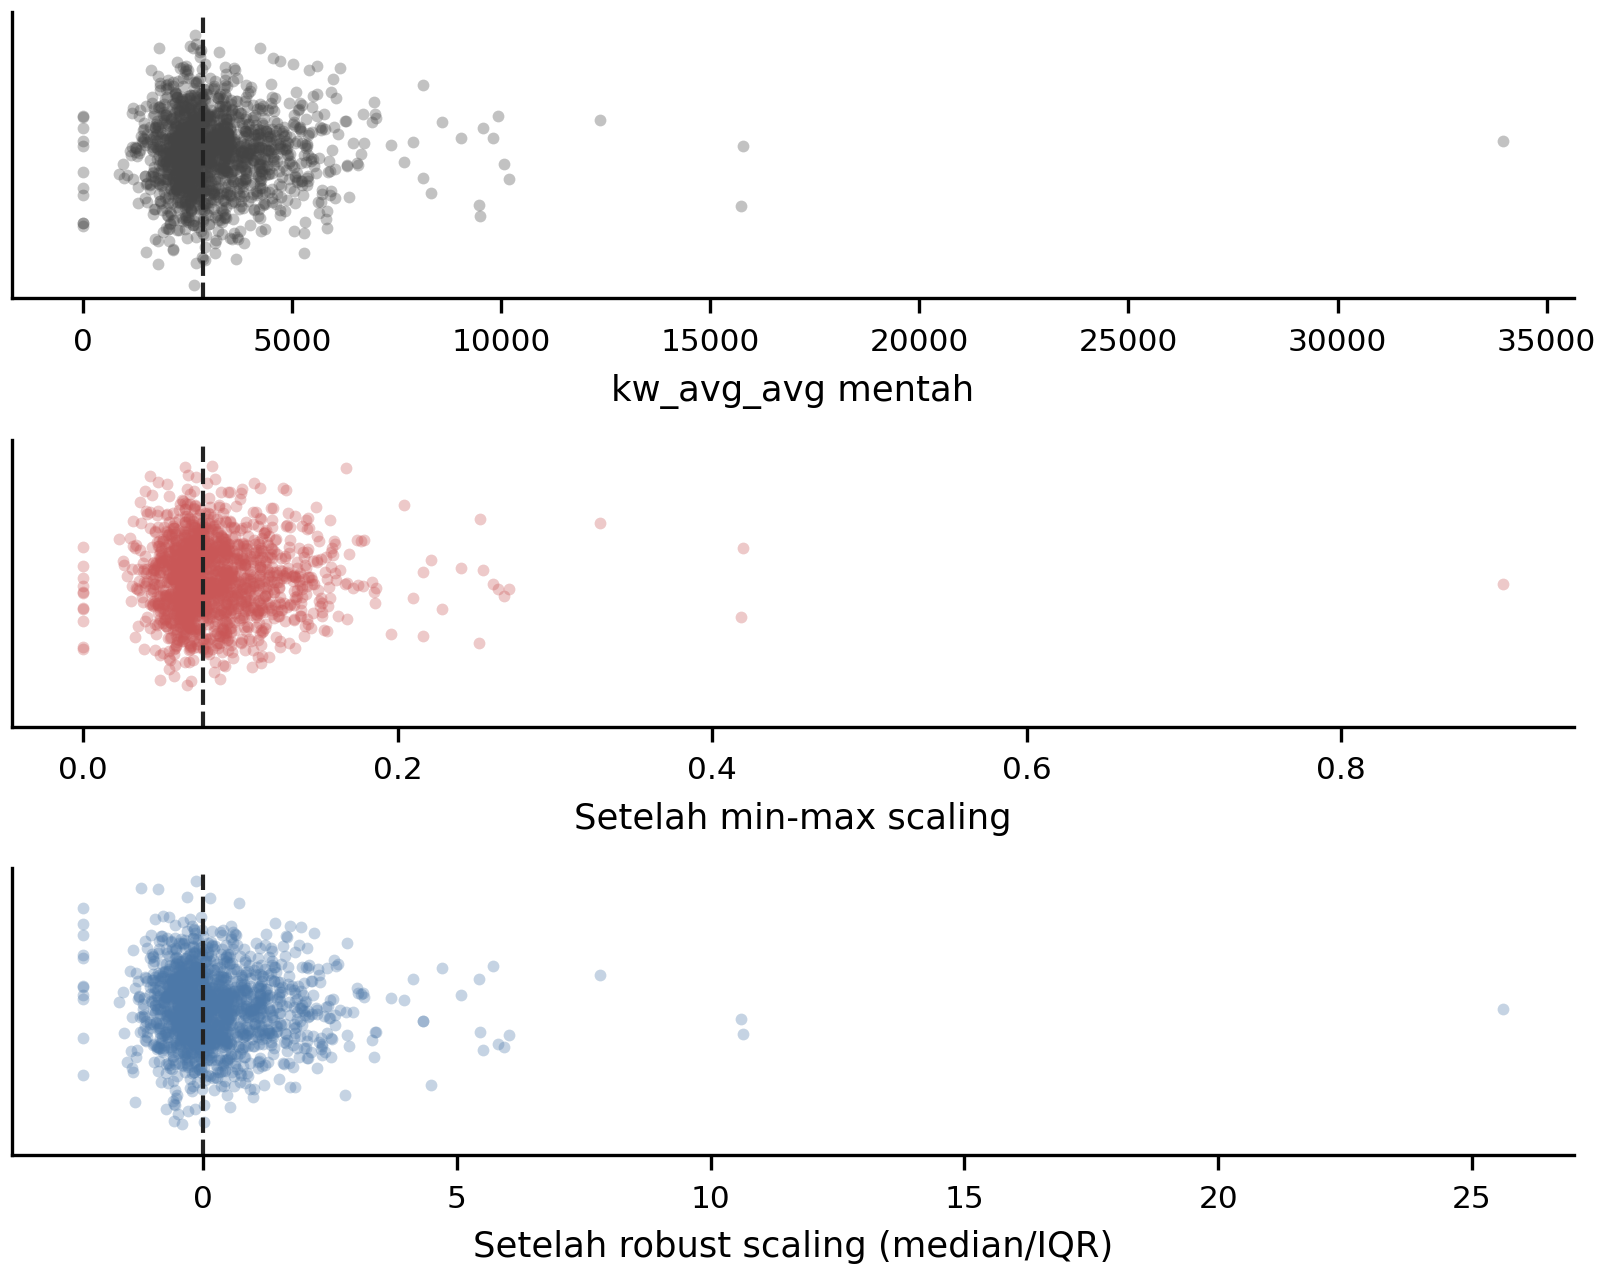
\includegraphics[width=\linewidth,height=0.72\textheight,keepaspectratio]{ch03-fig-3}
\caption{Alur Pemetaan Batas Interval Diskrit (Discretization/Binning)}
\label{fig:ch03-fig-3}
\end{figure}

Langkah pemotongan ini menjaga rentang distribusi tetap padat dan mencegah model (terutama model berbasis gradien atau jarak) memberikan bobot kesalahan yang tidak wajar akibat satu pengamatan ekstrem.

\section{Power dan Quantile Transform}\label{power-dan-quantile-transform}

Selain penyesuaian skala metrik, bentuk distribusi fitur numerik juga perlu diperbaiki. Model berbasis jarak atau gradien bekerja lebih baik bila data mendekati distribusi normal. Namun, sebagian besar observasi riil seperti harga atau pendapatan menceng (\emph{skewed}) dengan ekor panjang di satu sisi. Memasukkan data menceng secara langsung ke dalam model linier membuat model kesulitan membaca pola sentral.

Untuk menstabilkan varians dan mengurangi kemencengan, kita menggunakan \emph{power transform}. Transformasi ini menerapkan kompresi non-linier yang lebih kuat pada angka-angka besar, sehingga sebaran data yang berada di ujung ekor akan tertarik dan merapat ke pusat. Dua metode utama dalam teknik ini adalah transformasi Box-Cox (yang hanya mendukung data bernilai positif murni) dan Yeo-Johnson (yang mampu memproses angka bernilai nol atau negatif). Kedua metode ini bekerja secara algoritmis mengestimasi parameter kompresi optimal melalui pendekatan \emph{Maximum Likelihood Estimation} (MLE). Sebagai representasi, formula transformasi Box-Cox didefinisikan sebagai berikut:

\[
x_i^{(\lambda)} = 
\begin{cases} 
\frac{x_i^\lambda - 1}{\lambda} & \text{jika } \lambda \neq 0 \\ 
\ln(x_i) & \text{jika } \lambda = 0 
\end{cases}
\]

Di mana \(x_i\) merepresentasikan nilai fitur awal, dan \(\lambda\) adalah parameter kompresi yang disesuaikan dari data latih. Jika \(\lambda\) bernilai nol, metode ini menghasilkan bentuk transformasi logaritma natural biasa.

{[}GAMBAR 3.4: Plot Data - Q-Q plot efek transformasi Box-Cox pada data harga yang menceng{]}

Meskipun \emph{power transform} mampu mengkoreksi kemencengan, transformasi parametrik ini tetap rentan terdistorsi oleh \emph{outlier} ekstrem. Pendekatan alternatif yang kebal \emph{outlier} adalah \emph{quantile transform}.

\emph{Quantile transform} sepenuhnya membuang operasi aritmetika dan beroperasi menggunakan pemetaan urutan (\emph{rank}). Algoritmanya bekerja dengan mengurutkan peringkat nilai dari setiap observasi, memetakannya ke nilai probabilitas kumulatif, dan akhirnya mencetak ulang probabilitas tersebut ke dalam bentuk distribusi seragam (\emph{uniform}) atau distribusi normal.

Pemetaan berbasis kuantil ini menghasilkan beberapa kompromi praktis dalam desain fitur. Di satu sisi, pendekatan ini menawarkan kekebalan penuh terhadap \emph{outlier}, karena nilai observasi sebesar apa pun hanya akan sekadar menduduki peringkat teratas tanpa memengaruhi penyebaran mayoritas data. Di sisi lain, hal ini mengakibatkan distorsi jarak spasial karena jarak linier awal antar-titik data dihapus total. Transformasi ini juga dapat mengubah korelasi asli antar-fitur. Terakhir, \emph{quantile transform} memiliki batasan pada ukuran data; karena ia memetakan nilai berdasarkan empirisme sampel semata, metode ini rentan mengalami \emph{overfitting} pada \emph{dataset} berukuran kecil. Jika ukuran sampel hanya dalam rentang ratusan baris, pendekatan parametrik seperti \emph{power transform} selalu menjadi pilihan yang jauh lebih stabil.

\section{Clipping dan Discretization (Binning)}\label{clipping-dan-discretization-binning}

Transformasi matematis seperti logaritma atau standardisasi bukan satu-satunya cara memanipulasi sebaran numerik. Pendekatan lain beroperasi dengan membatasi rentang nilai secara absolut atau mengelompokkan presisi data ke dalam kategori interval.

\textbf{Clipping (Winsorization).}\label{clipping-winsorization}

\emph{Clipping} membatasi nilai mentah pada ambang minimum dan maksimum absolut. Nilai yang melewati batas ini ditekan agar sejajar dengan ambang tersebut, sehingga observasi \emph{outlier} tidak dibuang melainkan dipertahankan pada nilai ekstrem yang dikendalikan. Saat batas ini ditentukan melalui parameter statistik, teknik ini disebut \emph{winsorization}.

Proses pembatasan ini diformulasikan sebagai fungsi sepotong-sepotong (piecewise):

\[
x_{clip} = \begin{cases} \theta_{min} & \text{jika } x < \theta_{min} \\ x & \text{jika } \theta_{min} \le x \le \theta_{max} \\ \theta_{max} & \text{jika } x > \theta_{max} \end{cases}
\]

Keterangan:

\begin{itemize}
\tightlist
\item
  \(x\) mewakili observasi data numerik awal.
\item
  \(\theta_{min}\) adalah ambang batas bawah.
\item
  \(\theta_{max}\) adalah ambang batas atas.
\end{itemize}

Praktisi menentukan \(\theta_{min}\) dan \(\theta_{max}\) melalui tiga mekanisme utama. Pertama, berbasis persentil (\emph{quantiles}), di mana pemotongan distribusi bersandar pada batas persentil murni (misalnya membatasi populasi hanya pada rentang persentil ke-5 hingga ke-95). Kedua, berbasis Rentang Interkuartil (IQR), yakni menggunakan batas deteksi pencilan standar seperti \(Q_1 - 1.5 \times \text{IQR}\) untuk batas bawah dan \(Q_3 + 1.5 \times \text{IQR}\) untuk batas atas. Ketiga, berbasis \emph{Median Absolute Deviation} (MAD), yang mengukur dispersi dari median dan menetapkan batas berdasarkan kelipatannya (contohnya mematok batas atas pada nilai \(\text{Median} + 3.29 \times \text{MAD}\)). Perhitungan MAD terbukti jauh lebih kebal terhadap kontaminasi ekstrem jika dibandingkan dengan menggunakan IQR atau deviasi standar. Pendekatan \emph{clipping} pada akhirnya menjamin stabilitas karena mencegah \emph{outlier} mendominasi pembobotan algoritma, sembari tetap menjaga tanpa mendistorsi kepadatan data di area sentral (\emph{inliers}).

\textbf{Discretization (Binning).}\label{discretization-binning}

\emph{Discretization} mengubah fitur kontinu menjadi variabel kategorikal ordinal atau diskrit dengan melebur angka spesifik ke dalam interval batas (\emph{bins}).

{[}GAMBAR 3.5: Histogram - Perbandingan distribusi data umur kontinu sebelum dan sesudah dipetakan menjadi kelompok interval diskrit{]}

Penentuan lebar dan tepi batas interval dapat mengikuti beberapa strategi operasional. Strategi seragam (\emph{uniform}) membagi seluruh rentang nilai ke dalam jumlah interval dengan lebar jarak absolut yang sama, meski rentan menghasilkan banyak interval kosong jika data terlalu condong. Strategi kuantil (\emph{quantile}) memastikan setiap interval memiliki populasi observasi yang identik dengan menyesuaikan lebar jarak secara dinamis. Strategi k-Means menjalankan algoritma \emph{clustering} 1D untuk mendeteksi pusat pengelompokan yang paling natural berdasarkan kedekatan nilai. Terakhir, diskritisasi terarah (\emph{supervised discretization}) melatih satu pohon keputusan dangkal (kedalaman 2-4) khusus pada fitur kontinu tersebut demi memprediksi variabel target; daun dari pohon inilah yang akan ditetapkan sebagai interval diskrit. Metode terakhir ini menjamin batasan \emph{binning} berkorelasi langsung dengan daya prediksi model.

Proses \emph{discretization} ini sanggup mengubah asumsi arsitektur model secara drastis. Pada model linier (seperti regresi atau SVM linier), \emph{binning} menyuntikkan kemampuan untuk menangkap sinyal non-linier; model tidak lagi berasumsi bahwa perubahan satu unit angka akan berdampak konstan, melainkan menetapkan bobot unik pada setiap kategori interval (misalnya bobot usia 18-25 dipisah dengan bobot kelompok usia 26-40). Sebaliknya, pada algoritma berbasis pohon (\emph{random forest}, \emph{gradient boosting}), teknik \emph{binning} pra-pemrosesan konvensional ini jarang memberi nilai tambah karena mesin pohon memang sudah beroperasi dengan mencari titik pisah diskrit secara adaptif dan internal.

Sebagai evolusi modern dari teknik ini, transformasi \textbf{Spline} (\emph{Piecewise Polynomials}) mengatasi kelemahan utama \emph{binning}: batas interval yang kasar (efek tangga). \emph{Spline transformer} memproyeksikan fitur ke dalam basis polinomial derajat rendah, menciptakan transisi kurva yang kontinu melewati ambang batas interval. Pendekatan ini mempertahankan daya representasi non-linear model linier tanpa merusak gradien pada perbatasan antar kelompok observasi.

\section{Model yang Sensitif vs.~Tidak Sensitif terhadap Skala}\label{model-yang-sensitif-vs.-tidak-sensitif-terhadap-skala}

Transformasi nilai seperti \emph{standardization} atau \emph{min-max scaling} bukanlah tahap wajib untuk semua algoritma \emph{machine learning}. Keputusan menerapkan pengubahan skala bergantung pada arsitektur perhitungan yang digunakan. Praktisi membagi model ke dalam dua kelompok berdasarkan tingkat sensitivitasnya terhadap parameter skala.

\textbf{Model yang Sensitif terhadap Skala.}\label{model-yang-sensitif-terhadap-skala}

Model dalam kategori ini sangat bergantung pada rentang nilai absolut dari sebuah fitur. Jika satu fitur memiliki rentang numerik hingga jutaan (seperti pendapatan) sedangkan fitur lain hanya berskala puluhan (seperti usia), fitur dengan angka besar akan mendominasi hasil prediksi.

Model yang sensitif terbagi menjadi dua keluarga perhitungan. Keluarga pertama adalah model berbasis jarak (\emph{metric-based estimators}), seperti \emph{k-Nearest Neighbors} (k-NN) dan \emph{Support Vector Machine} (SVM) yang mengukur kedekatan antar-titik data secara spasial. Selisih jarak komputasi dari fitur yang berskala jutaan akan menelan kontribusi fitur lain yang angkanya lebih kecil. Keluarga kedua adalah model berbasis gradien (\emph{gradient-based estimators}), seperti regresi linier dan \emph{neural networks} yang memperbarui bobot parameter menggunakan fungsi turunan. Perbedaan skala fitur yang tajam akan melencengkan arah pencarian dan memperlambat konvergensi, bahkan berisiko membuat algoritma optimasi gagal menemukan titik minimum (\emph{error} terkecil).

Untuk mencegah fitur dominan merusak prediksi, praktisi menormalkan skala menggunakan metode seperti \emph{Standard Scaler}. Transformasi ini mengubah nilai asli fitur menjadi skor \emph{Z-score}:

\[ z = \frac{x - \mu}{\sigma} \]

Di mana \(z\) mewakili nilai hasil transformasi, \(x\) adalah angka fitur mentah, \(\mu\) adalah rata-rata fitur, dan \(\sigma\) adalah standar deviasi fitur tersebut. Proses ini memastikan setiap dimensi beroperasi pada skala matematika yang seragam sebelum masuk ke tahap pelatihan.

{[}GAMBAR 3.6: Skema - Skema scaling (MinMax vs Standard) yang menormalkan rentang angka antar dimensi fitur{]}

\textbf{Model yang Tidak Sensitif terhadap Skala.}\label{model-yang-tidak-sensitif-terhadap-skala}

Keluarga \textbf{model berbasis pohon (\emph{tree-based estimators})} memiliki karakteristik yang sama sekali tidak terpengaruh oleh besaran skala fitur. Kategori ini mencakup \emph{Decision Trees}, \emph{Random Forest}, dan \emph{Gradient Boosting}.

Ada beberapa karakteristik yang membuat model pohon dikategorikan kebal terhadap perbedaan skala. Pertama, model melakukan pembelahan secara ordinal. Pohon keputusan memproses variabel secara independen dan mencari titik potong secara berurutan (misalnya sekadar mengevaluasi kondisi \passthrough{\lstinline!Usia < 30!}). Algoritma tidak pernah menjumlahkan atau mengalikan magnitudo antar-fitur dalam satu fungsi matematis. Kedua, adanya kuantisasi internal. Pustaka \emph{gradient boosting} modern (seperti LightGBM atau XGBoost) telah mengintegrasikan teknik pemilahan otomatis (\emph{histogram-based binning}) yang mengelompokkan urutan nilai kontinu ke dalam rentang keranjang (\emph{bin}) yang diskret. Batas pembagian cabang pada pohon pun dicari semata-mata berdasarkan rentang keranjang tersebut, membuat model pada dasarnya netral terhadap besaran nominal aslinya (\emph{scale-invariant}). Oleh karenanya, praktisi dapat menyuapkan data numerik mentah ke dalam model berbasis pohon tanpa melakukan \emph{scaling} sama sekali, namun tetap akan mendapatkan hasil prediksi yang identik secara matematis dengan skenario data terskala.

\section{Studi Kasus: Efek Transformasi pada Berbagai Keluarga Model}\label{studi-kasus-efek-transformasi-pada-berbagai-keluarga-model}

Untuk melihat dampak skala fitur secara langsung, kita menguji sebuah \emph{dataset} dengan dua atribut numerik yang rentangnya sangat asimetris: atribut gaji yang bernilai puluhan juta rupiah dan pengalaman kerja yang diukur dalam hitungan tahun. Pengujian ini membandingkan daya prediksi tiga keluarga algoritma (\emph{k-Nearest Neighbors} (k-NN), \emph{Support Vector Machine} (SVM), dan \emph{Random Forest}) menggunakan set data mentah dan data yang telah melewati proses standardisasi.

Hasil evaluasi pada data mentah menunjukkan bahwa k-NN dan SVM mengalami degradasi akurasi yang signifikan. Kedua algoritma ini termasuk dalam kelompok model berbasis metrik (\emph{metric-based estimators}), yang cara kerjanya sangat mengandalkan perhitungan jarak spasial antar titik observasi di ruang berdimensi tinggi.

Akar masalah degradasi ini terlihat jelas dari definisi matematis jarak Euclidean:

\[ d(\mathbf{x}, \mathbf{x}') = \sqrt{\sum_{i=1}^{d} (x_i - x'_i)^2} \]

Keterangan:

\begin{itemize}
\tightlist
\item
  \(d(\mathbf{x}, \mathbf{x}')\) melambangkan jarak spasial antara titik \(\mathbf{x}\) dan observasi \(\mathbf{x}'\).
\item
  \(x_i\) dan \(x'_i\) adalah nilai dari fitur ke-\(i\).
\item
  \(d\) mewakili total jumlah dimensi atau fitur.
\end{itemize}

Berdasarkan rumus di atas, atribut gaji dengan nilai varians dalam orde jutaan akan memproduksi selisih kuadrat yang masif. Angka ini secara otomatis mendominasi seluruh hasil kalkulasi jarak spasial. Akibatnya, perbedaan pengalaman kerja sebesar apa pun akan tenggelam dan kehilangan bobot prediktifnya.

Ketika kita menyisipkan komponen standardisasi ke dalam \emph{pipeline} untuk memaksa fitur berada pada rentang yang seragam, ruang Euclidean tersebut tidak lagi dikuasai oleh satu variabel. Hasilnya, akurasi k-NN dan SVM langsung melonjak drastis karena sistem penalti jarak kini memproses setiap fitur secara proporsional.

Di sisi lain, algoritma \emph{Random Forest} menunjukkan karakteristik respons yang sepenuhnya berbeda, karena ia masuk dalam keluarga model berbasis pohon (\emph{tree-based estimators}). Model ini terbukti kebal terhadap perbedaan rentang; performanya bernilai persis sama, baik saat memproses data mentah yang sangat asimetris maupun data yang telah distandardisasi. Hal ini terjadi berkat mekanisme pencarian titik potong pohon keputusan yang mencari \emph{threshold} percabangan optimal murni berdasarkan urutan peringkat pada satu fitur tunggal, bukan dengan cara mengkalkulasi jarak kombinasi antar-fitur. Selain itu, banyak implementasi algoritma pohon modern menerapkan teknik \emph{histogram-based binning}, di mana semua deret fitur kontinu akan dikuantisasi ke dalam interval diskret internal. Karakteristik ini membuat algoritma sepenuhnya kebal terhadap magnitudo aslinya. Karena standardisasi pada dasarnya hanya mentransformasi skala (bukan mengubah urutan peringkat observasi), topologi percabangan pohon yang terbangun dari data mentah tidak akan pernah menyimpang dari struktur pohon data berskala.

{[}GAMBAR 3.7: Plot Data - Grafik batang komparatif yang menampilkan lonjakan akurasi k-NN dan SVM pasca-standardisasi, sementara performa Random Forest tetap statis tak berubah{]}

Eksperimen komparatif ini menghasilkan panduan praktis yang dapat langsung diadopsi. Kita wajib menyertakan standardisasi sebelum melatih model berbasis metrik spasial (seperti k-NN dan SVM) maupun model yang menggunakan optimasi gradien (seperti regresi linier dan jaringan saraf tiruan, di mana data tak berskala sangat menghambat laju konvergensi). Sebaliknya, kita dapat melewati tahap prapemrosesan ini sepenuhnya jika \emph{pipeline} dirancang menggunakan keluarga algoritma berbasis pohon (seperti \emph{Random Forest}, XGBoost, atau LightGBM). Menghilangkan modul penskalaan saat menggunakan pohon keputusan akan membebaskan sistem dari kalkulasi yang tidak berguna, memastikan eksekusi komputasi lebih efisien tanpa mengorbankan kualitas akurasi sedikit pun.

\section{Sintesis Keputusan dan Prinsip Akhir}\label{sintesis-keputusan-dan-prinsip-akhir}

Manipulasi terhadap rentang skala dan bentuk distribusi fitur numerik adalah keputusan desain yang harus didasarkan pada karakteristik arsitektur model dan sebaran asli data.

\textbf{Panduan Pemilihan Penskalaan.} Standardisasi merupakan pilihan utama untuk model parametrik, model linear, dan algoritma berbasis gradien atau metrik jarak (seperti k-NN dan SVM), terutama saat data terdistribusi normal atau mendekati simetris. Skala min-max lebih tepat digunakan untuk algoritma yang memproses input dalam rentang tertutup yang konstan (seperti pengolahan intensitas piksel citra digital). Jika data mengandung banyak pencilan ekstrem, terapkan \emph{robust scaling} menggunakan median dan IQR agar penyebaran kelompok data utama tidak terdistorsi.

\textbf{Koreksi Distribusi.} Sebaran data yang menceng dengan ekor panjang ditarik menuju sebaran normal menggunakan \emph{power transform} (seperti Box-Cox atau Yeo-Johnson). Untuk kekebalan penuh terhadap pencilan dengan konsekuensi distorsi jarak spasial asli, \emph{quantile transform} adalah alternatif non-parametrik yang tangguh. Batasi rentang nilai secara absolut menggunakan teknik \emph{clipping} untuk meredam keliaran anomali ekstrem tanpa membuang baris observasinya.

\textbf{Sensitivitas Algoritma.} Keluarga model berbasis pohon (seperti \emph{random forest} dan \emph{gradient boosting}) sepenuhnya kebal terhadap perbedaan skala fitur karena proses percabangannya bekerja secara ordinal dan independen pada setiap kolom. Menghilangkan tahapan penskalaan saat menggunakan model pohon membebaskan sistem dari komputasi redundan di lingkungan produksi.

Latihan praktis dan eksperimen pengujian efek penskalaan pada berbagai keluarga model secara interaktif dapat diakses pada dokumen naskah pendamping di repositori buku ini.

% ==========================================================================
% ch04.tex — dihasilkan dari v2/drafts oleh tools/md2tex.py
% Sumber: v2\drafts\ch04\ch04_draft_v2.md
% Boleh disunting manual; menjalankan md2tex.py lagi akan menimpa.
% ==========================================================================
\chapter{Representasi Fitur Kategorikal}\label{representasi-fitur-kategorikal}

Banyak tabel tidak hanya berisi angka. Di dalamnya terdapat pekerjaan, wilayah, status rumah tangga, negara lahir, jenis kelamin, atau tingkat pendidikan. Sebagian kolom hanya memberi nama kelompok. Sebagian mempunyai urutan. Sebagian lain mempunyai banyak level, seperti negara lahir atau kode pekerjaan rinci. Bagi model, label harus diubah menjadi angka tanpa merusak maknanya. Jika kategori diberi angka secara sembarang, angka itu mudah disalahpahami sebagai urutan atau jarak. Jika setiap kombinasi dibuat menjadi kolom sendiri, matriks fitur dapat menjadi sangat lebar dan jarang.

Pengodean fitur kategorikal bukan pekerjaan mekanis. Encoder yang baik menjawab makna apa yang dipertahankan, seberapa besar dimensi keluarannya, apa yang terjadi ketika kategori baru muncul, dan risiko bagi validasi. Bab ini membahas one-hot encoding, ordinal encoding, pengodean berbasis frekuensi, pengodean berbasis target (target encoding) beserta risiko kebocorannya, hashing untuk kardinalitas tinggi, entity embedding, dan penanganan kategori tak dikenal saat inferensi.

\section{Jenis Variabel Kategorikal}\label{jenis-variabel-kategorikal}

Variabel kategorikal berisi nilai yang menyatakan kelompok, jenis, label, atau identitas. Arti kategori berasal dari domain, bukan hanya dari tipe data di komputer.

Contoh kerja pada bab ini menggunakan dataset Census-Income, yang berisi catatan individu dari survei penduduk Amerika Serikat. Setiap baris memuat informasi seperti pendidikan, status perkawinan, negara lahir, jenis pekerjaan, dan kode industri. Kolom-kolom tersebut digunakan untuk memperkirakan kelompok pendapatan. Contoh ini mempertemukan kategori nominal, ordinal, dan kategori dengan kardinalitas yang berbeda dalam satu tabel.

Dalam dataset ini, kode industri atau pekerjaan dapat tersimpan sebagai angka, tetapi tetap kategorikal. Sebaliknya, tingkat pendidikan tersimpan sebagai teks, tetapi mempunyai urutan yang jelas.

Kategori nominal tidak memiliki urutan alami. Negara lahir, ras, jenis pekerjaan, industri, dan status rumah tangga adalah contoh umum. Kita tidak dapat mengatakan bahwa satu negara lahir ``lebih besar'' daripada negara lain hanya karena diberi kode angka lebih tinggi. Kategori ordinal mempunyai urutan yang bermakna, misalnya tingkat pendidikan dari sekolah dasar sampai doktoral, kelas risiko rendah \textless{} sedang \textless{} tinggi, atau rating kepuasan 1 sampai 5. Kategori biner adalah kasus khusus dengan dua nilai, misalnya ya/tidak atau perempuan/laki-laki, tetapi tetap harus dikodekan secara konsisten.

Kardinalitas adalah jumlah nilai kategori yang berbeda. Kolom jenis kelamin memiliki kardinalitas rendah. Kolom pendidikan memiliki belasan level. Kolom negara lahir, status rumah tangga, kode industri, dan kode pekerjaan dapat memiliki puluhan level. Jika beberapa kolom digabung menjadi satu kategori turunan, jumlah level dapat melonjak jauh lebih besar. Kardinalitas menentukan biaya representasi. Encoder yang cocok untuk lima kategori belum tentu cocok untuk ribuan kombinasi kategori.

Secara umum, encoder dapat dilihat sebagai pemetaan dari kosakata kategori ke ruang numerik.

\[
f_{\text{encode}} : \mathcal{V} \rightarrow \mathbb{R}^d
\]

Dengan \(\mathcal{V}\) sebagai himpunan nilai kategori yang dikenal dari data \emph{train} dan \(d\) sebagai dimensi keluaran, setiap encoder membuat kompromi yang berbeda. Pada ordinal encoding, biasanya \(d = 1\). Pada \emph{one-hot encoding}, \(d = |\mathcal{V}|\), yaitu satu kolom untuk setiap kategori. Pada hashing dan \emph{embedding}, \(d\) dipilih sebagai ukuran representasi yang tetap.

Kerangka ini membantu membandingkan seluruh metode dalam bab ini. Perbandingan dapat dilihat dari informasi kategori yang dipertahankan, informasi yang dikompresi, perlakuan terhadap kategori baru, serta risiko bagi model dan \emph{pipeline}. Pertimbangan tersebut lebih penting daripada menghafal nama encoder.

\section{\texorpdfstring{\emph{One-Hot} dan Ordinal Encoding}{One-Hot dan Ordinal Encoding}}\label{one-hot-dan-ordinal-encoding}

Kasus paling dasar adalah memilih apakah kategori harus tetap terpisah atau boleh diberi urutan. Dua encoder yang sering muncul adalah \emph{one-hot encoding} dan ordinal encoding. Keduanya sama-sama mengubah kategori menjadi angka, tetapi asumsi yang dibawa berbeda.

\emph{One-hot encoding} membuat satu kolom indikator untuk setiap kategori. Jika kolom status perkawinan pada Census-Income memiliki tiga kategori contoh, ``Never married'', ``Married-civ-spouse'', dan ``Divorced'', maka nilai ``Never married'' dapat ditulis sebagai berikut.

\[
\mathbf{x} = [x_1, \dots, x_K] \in \{0,1\}^K
\]

dengan tepat satu \(x_i = 1\). Untuk contoh tadi, ``Never married'' pada urutan \{Never married, Married-civ-spouse, Divorced\} menjadi \([1, 0, 0]\). Representasi ini tidak memaksakan urutan. Ketiga status perkawinan tersebut diperlakukan sebagai kategori terpisah.

\emph{One-hot encoding} cocok untuk kardinalitas rendah sampai menengah. Kelemahannya muncul ketika jumlah kategori besar. Jika kode pekerjaan rinci, negara lahir, dan status rumah tangga digabung menjadi satu kategori turunan, \emph{one-hot} dapat menghasilkan ribuan kolom biner, sebagian besar bernilai nol. Matriks menjadi lebar, jarang, dan dapat membebani memori serta model.

Ordinal encoding memetakan kategori ke satu kolom integer. Untuk variabel yang benar-benar berurutan, cara ini wajar. Tingkat pendidikan dapat diberi kode berurutan karena relasi urutnya memang bermakna. Namun, untuk kategori nominal seperti negara lahir atau kode pekerjaan, kode 1, 2, 3 dapat menyesatkan. Model linear atau berbasis jarak dapat membaca kode yang lebih besar sebagai kategori yang lebih tinggi atau lebih jauh, padahal angka itu hanya label buatan.

Gambar 4.1 memperlihatkan perbedaan ini. Ordinal encoding hemat dimensi, tetapi membawa asumsi urutan. \emph{One-hot encoding} lebih lebar, tetapi menjaga kategori tetap terpisah.

\begin{figure}[tbp]\centering
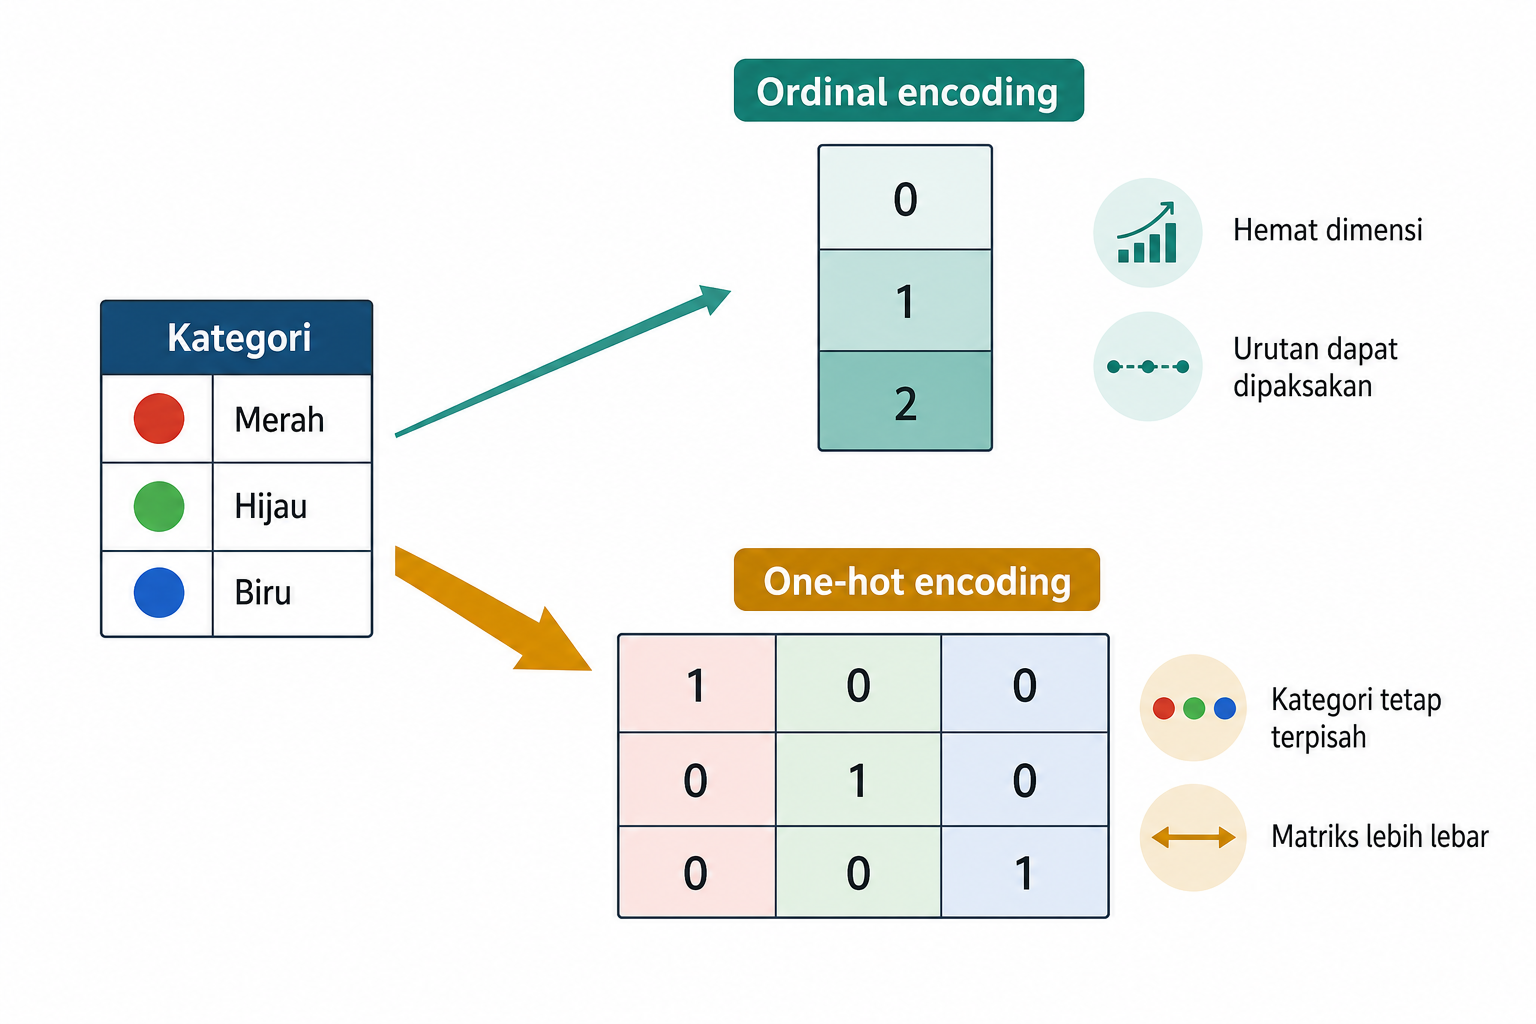
\includegraphics[width=111.6mm]{ch04-fig-1}
\caption{One-hot dan ordinal encoding pada kolom kategori}
\label{fig:ch04-fig-1}
\end{figure}

Baik \emph{one-hot} maupun ordinal encoder mempelajari pemetaan dari data \emph{train}. Pada data baru, kategori harus mengikuti pemetaan yang sama. Pada \passthrough{\lstinline!OneHotEncoder!}, parameter \passthrough{\lstinline!handle_unknown!} seperti \passthrough{\lstinline!'error'!}, \passthrough{\lstinline!'ignore'!}, \passthrough{\lstinline!'infrequent_if_exist'!}, atau \passthrough{\lstinline!'warn'!}, serta \passthrough{\lstinline!min_frequency!} dan \passthrough{\lstinline!max_categories!}, menentukan perilaku terhadap kategori baru dan kategori jarang. Pada \passthrough{\lstinline!OrdinalEncoder!}, \passthrough{\lstinline!handle_unknown!}, misalnya \passthrough{\lstinline!'error'!} atau \passthrough{\lstinline!'use_encoded_value'!}, bersama \passthrough{\lstinline!unknown_value!} dan \passthrough{\lstinline!encoded_missing_value!} memainkan peran serupa.

Untuk model linear tanpa \emph{regularization}, \passthrough{\lstinline!drop='first'!} atau \passthrough{\lstinline!drop='if_binary'!} dapat dipakai untuk menghindari kolinearitas sempurna antarkolom \emph{one-hot}, meskipun penghapusan ini membuat representasi kehilangan simetri antarkategori. Jika \passthrough{\lstinline!handle_unknown='ignore'!} menghasilkan baris \emph{all-zero}, kategori tak dikenal tidak dapat dibedakan dari kategori referensi yang dibuang oleh \passthrough{\lstinline!drop='first'!}, karena keduanya mempunyai kode yang sama. Ketika pembedaan tersebut penting, siapkan bucket eksplisit untuk kategori tak dikenal atau jarang saat \emph{fit}, atau pantau laju kategori baru, bukan hanya mengandalkan kode \emph{all-zero}. \passthrough{\lstinline!OrdinalEncoder!} juga berbeda dari \passthrough{\lstinline!LabelEncoder!}. Yang pertama didesain untuk kolom fitur dan menerima \emph{input} 2-D, sedangkan yang kedua dimaksudkan untuk label target. Setelah makna dasar kategori dijaga, persoalan berikutnya adalah skala karena beberapa kolom terlalu besar untuk diperlakukan dengan \emph{one-hot} biasa.

\begin{pendalaman}{Nilai kosong dan kategori tak dikenal sebagai kebijakan encoder}
Nilai kosong pada fitur kategorikal tidak selalu harus dihapus atau diimputasi menjadi kategori paling sering. Pada beberapa encoder, nilai kosong dapat diperlakukan sebagai kategori tersendiri. \passthrough{\lstinline!OrdinalEncoder(encoded_missing_value=...)!}, misalnya, dapat memetakan NaN ke integer khusus secara deterministik. Sementara itu, \passthrough{\lstinline!handle_unknown!} menentukan apa yang terjadi ketika kategori baru muncul saat inferensi, mulai dari error, baris all-zero, kode khusus, sampai masuk ke bucket infrequent. Semua ini adalah kebijakan desain yang harus diputuskan saat \emph{fit}, bukan perilaku default yang baru ditemukan ketika sistem sudah berjalan. Bagian 4.7 membahas kategori baru lebih lengkap, sedangkan Bab 5 membahas kebijakan nilai kosong.
\end{pendalaman}

\section{Count Encoding dan Frequency Encoding}\label{count-encoding-dan-frequency-encoding}

Ketika kategori sangat banyak, \emph{one-hot encoding} dapat menjadi terlalu lebar. Count encoding dan frequency encoding menawarkan kompresi sederhana. Count encoding mengganti setiap kategori dengan jumlah kemunculannya pada data \emph{train}. Frequency encoding menggantinya dengan proporsi kemunculan.

\[
f(c) = \frac{N(c)}{N_{\text{train}}}
\]

Dengan \(N(c)\) sebagai jumlah baris \emph{train} dengan kategori \(c\) dan \(N_{\text{train}}\) sebagai jumlah baris \emph{train}, kategori yang sering muncul mendapat nilai lebih besar. Jika sebuah kode pekerjaan muncul pada 2.000 dari 100.000 baris pelatihan, frequency encoding memberi nilai 0,02 untuk kode tersebut.

Metode ini terutama menjawab masalah dimensi keluaran. Kode pekerjaan, negara lahir, atau kategori rumah tangga yang jumlah levelnya besar dapat diringkas tanpa menambah banyak kolom. Nilai frekuensi juga kadang membawa sinyal. Kategori yang sering muncul mungkin berbeda perilakunya dari kategori yang sangat jarang.

Namun, kompresi tersebut kehilangan banyak informasi. Dua negara lahir atau dua kode pekerjaan yang sama-sama muncul 150 kali akan mendapat nilai yang sama, meskipun maknanya berbeda. Bagi model, keduanya menjadi tidak dapat dibedakan melalui fitur ini. Count dan frequency encoding menyatakan seberapa umum sebuah kategori, bukan apa makna kategori tersebut.

Seperti encoder lain, pemetaan count atau frekuensi dipelajari dari data \emph{train}. Jika kategori baru muncul pada inferensi, tidak ada count yang tersimpan untuk kategori itu. Perilakunya bergantung pada konfigurasi encoder dan dapat berupa error, isian nol, nilai default, atau kebijakan khusus, misalnya lewat parameter seperti \passthrough{\lstinline!unseen!} pada \passthrough{\lstinline!CountFrequencyEncoder!} dari feature-engine. Karena itu, jangan menganggap kategori baru otomatis aman hanya karena keluarannya satu kolom.

Count dan frequency encoding paling berguna sebagai \emph{baseline} kompak untuk kardinalitas tinggi. Metode ini juga dapat digabung dengan pendekatan lain, misalnya \emph{rare category grouping} atau \emph{target encoding}. Jika hubungan kategori dengan target bergantung pada identitas spesifik kategori, kompresi berbasis frekuensi saja mungkin terlalu kasar. Dalam keadaan seperti itu, sebagian informasi target dapat dipakai sebagai ringkasan kategori, tetapi pengendalian \emph{leakage} harus ketat.

\section{\texorpdfstring{\emph{Target Encoding} dan Risiko \emph{Leakage}}{Target Encoding dan Risiko Leakage}}\label{target-encoding-dan-risiko-leakage}

Jika kompresi berbasis frekuensi terlalu kasar, informasi yang paling menggoda adalah hubungan kategori dengan target. \emph{Target encoding} melangkah ke arah itu dengan mengganti kategori menggunakan statistik target pada kategori tersebut. Pada klasifikasi pendapatan, misalnya, kode pekerjaan atau kategori pendidikan dapat diganti dengan rata-rata label \passthrough{\lstinline!income_gt_50k!} pada kategori itu. Untuk kategori berkardinalitas tinggi, satu angka seperti ini dapat menangkap asosiasi kategori dengan target tanpa membuat ribuan kolom.

Kekuatannya sekaligus menjadi bahayanya. \emph{Target encoding} memakai target untuk membuat fitur. Jika dilakukan secara naif pada seluruh data, label yang seharusnya diprediksi ikut masuk ke representasi. Model kemudian tampak sangat baik karena sebagian jawaban sudah tertanam di dalam fitur.

Ada dua pengaman utama, yaitu smoothing dan cross-fitting. Smoothing menahan kategori langka agar tidak terlalu percaya pada rata-rata targetnya sendiri. Salah satu bentuknya (Micci-Barreca 2001) ditulis sebagai berikut.

\[
S_i = \lambda_i\, \bar{y}_i + (1 - \lambda_i)\, \bar{y}_{\text{global}}, \qquad \lambda_i = \frac{n_i}{n_i + m}
\]

Dengan \(\bar{y}_i\) sebagai rata-rata target kategori \(i\) pada data \emph{train}, \(\bar{y}_{\text{global}}\) sebagai rata-rata target keseluruhan data \emph{train}, \(n_i\) sebagai jumlah contoh pada kategori \(i\), dan \(m\) sebagai kekuatan smoothing, nilai \(S_i\) menjadi campuran antara rata-rata kategori dan rata-rata global. Jika kategori sering muncul, \(n_i\) besar dan \(\lambda_i\) mendekati 1, sehingga rata-rata kategori lebih dipercaya. Jika kategori jarang muncul, \(\lambda_i\) mendekati 0, sehingga nilainya menyusut ke rata-rata global. Pada \passthrough{\lstinline!TargetEncoder!} scikit-learn, \passthrough{\lstinline!smooth='auto'!} menggunakan estimasi \emph{empirical Bayes} untuk memilih kekuatan smoothing secara otomatis. Nilai \passthrough{\lstinline!smooth!} numerik tertentu menetapkan kekuatan smoothing secara eksplisit.

Cross-fitting menghindari encoding yang melihat label barisnya sendiri. Data \emph{train} dibagi menjadi beberapa fold internal. Untuk setiap fold, encoding baris-baris di fold tersebut dihitung dari target pada fold lain. Dengan begitu, satu baris tidak pernah dikodekan memakai targetnya sendiri. Pada scikit-learn, \passthrough{\lstinline!TargetEncoder.fit_transform(X_train, y_train)!} melakukan cross-fitting internal, sedangkan \passthrough{\lstinline!fit(X_train, y_train).transform(X_train)!} tidak. \emph{Pipeline} yang di-\emph{fit} harus menghasilkan encoding pelatihan melalui jalur cross-fitted tersebut, kemudian memakai pemetaan yang dipelajari dari data \emph{train} untuk validasi, \emph{test}, dan inferensi. Kategori yang belum pernah terlihat biasanya diarahkan ke rata-rata global.

Gambar 4.2 memperlihatkan mekanisme itu. Perhatikan bahwa target dari fold yang sedang dienkode tidak masuk ke perhitungan encoding fold tersebut. Inilah hubungan langsung \emph{target encoding} dengan praktik \emph{pipeline} yang benar.

\begin{figure}[tbp]\centering
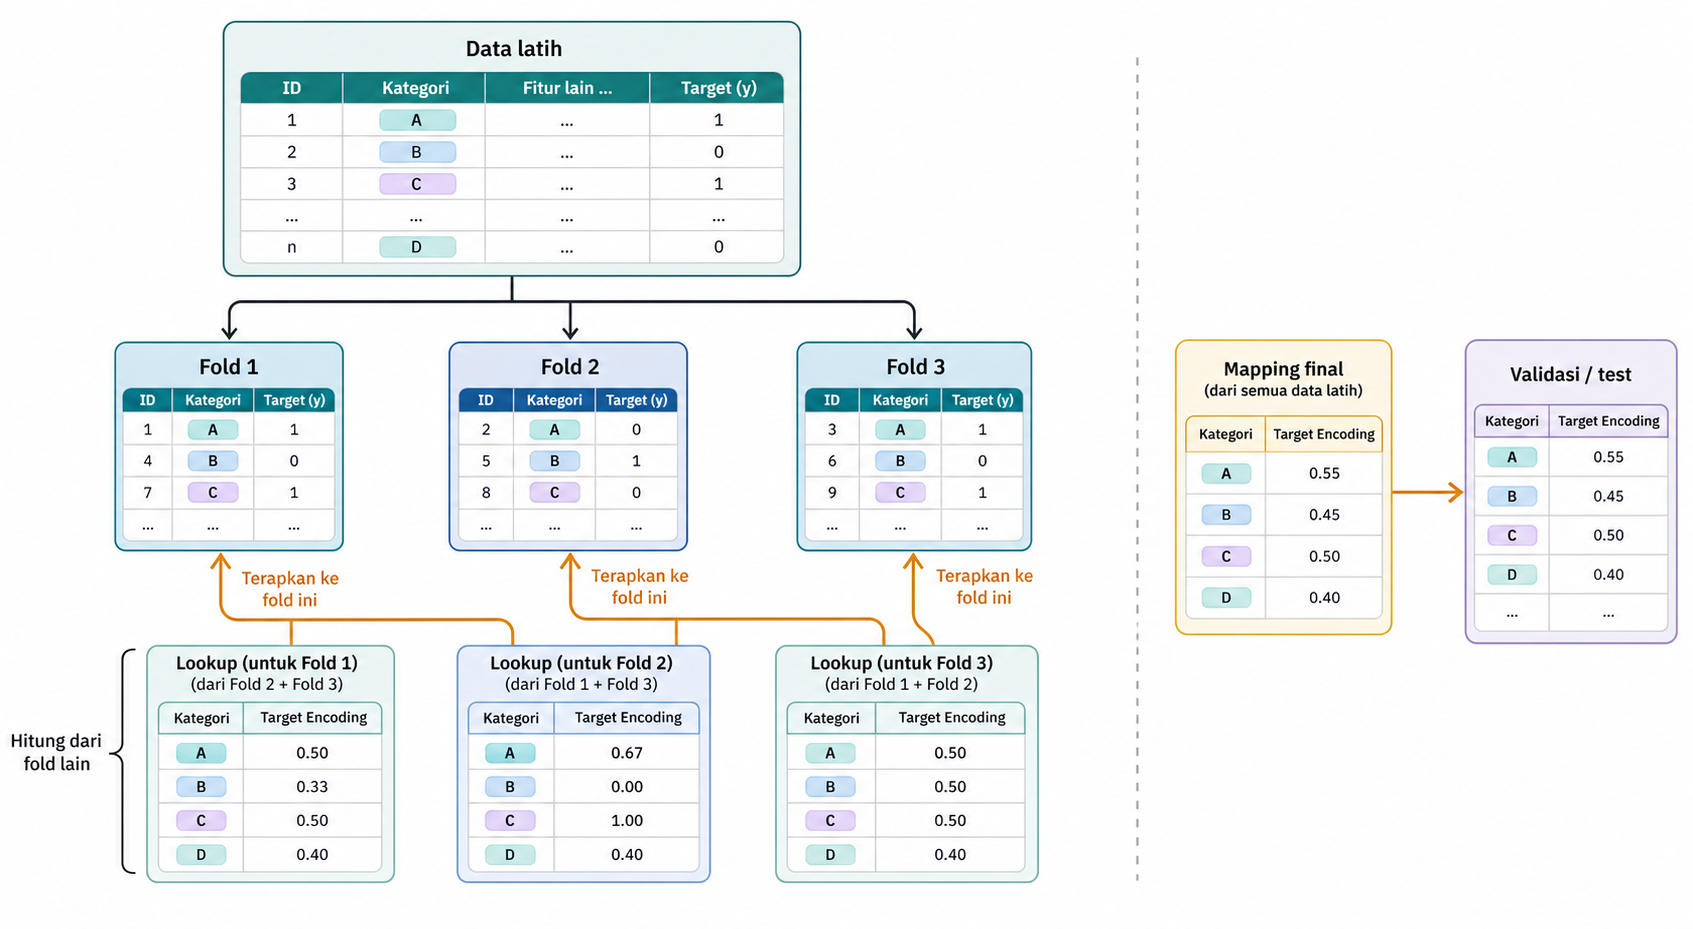
\includegraphics[width=111.6mm]{ch04-fig-2}
\caption{Cross-fitting untuk target encoding}
\label{fig:ch04-fig-2}
\end{figure}

\emph{Target encoding} sangat berguna, tetapi sebaiknya diperlakukan sebagai encoder berisiko tinggi. Encoder ini cocok untuk kategori banyak, tetapi harus selalu dipasang di dalam \emph{pipeline} validasi. Untuk kategori sangat jarang, grouping atau smoothing tambahan sering diperlukan agar nilai target mean tidak menjadi \emph{noise} yang diperlakukan terlalu serius oleh model. Ketika kosakata kategori sangat dinamis atau tidak ingin disimpan secara eksplisit, pendekatan berikutnya memilih kompresi yang lebih mekanis melalui hashing.

\begin{pendalaman}{Ordered target statistics ala CatBoost}
CatBoost mengendalikan \emph{target leakage} dengan mekanisme berbeda. Alih-alih membuat fold internal seperti cross-fitting, CatBoost memberi urutan acak pada baris pelatihan. Encoding untuk satu baris dihitung hanya dari baris-baris yang muncul lebih awal dalam urutan itu. Jadi, label baris tersebut tidak ikut membentuk encoding-nya sendiri. Tujuannya sama dengan cross-fitting, yaitu menghindari encoding yang self-referential, tetapi mekanismenya tertanam di dalam model. Inilah salah satu alasan CatBoost dapat menangani kolom kategorikal mentah secara native.
\end{pendalaman}

\section{Hashing untuk Fitur Berkardinalitas Tinggi}\label{hashing-untuk-fitur-berkardinalitas-tinggi}

Pada beberapa sistem, jumlah kategori bukan hanya besar, tetapi terus tumbuh. Kode wilayah, kode pekerjaan, atau kategori administratif baru dapat muncul setelah model dilatih. Menyimpan kosakata lengkap menjadi mahal, dan memperbarui encoder setiap kali kategori baru muncul tidak selalu praktis. Hashing memberi jalan lain.

Hashing memetakan string kategori ke sejumlah kolom tetap. Mekanisme ini menjawab dua kebutuhan sekaligus. Dimensi keluaran dibatasi sejak awal, dan kategori baru tetap dapat diproses tanpa memperluas kosakata. Rumus indeksnya dapat ditulis sebagai berikut.

\[
\text{indeks}(c) = \operatorname{hash}(c) \bmod k
\]

Dengan \(c\) sebagai kategori, fungsi \(\operatorname{hash}\) mengubah string kategori menjadi bilangan, dan \(k\) sebagai jumlah bucket atau kolom keluaran, hasil modulo menentukan kategori masuk ke kolom mana. Implementasi umum memakai MurmurHash3. Karena tidak ada kosakata yang disimpan, kategori baru dapat langsung diproses. String baru tetap dapat di-hash ke salah satu bucket.

Kelemahan hashing adalah collision. Dua kategori berbeda dapat masuk ke bucket yang sama. Collision bukan bug, melainkan harga dari ukuran keluaran yang tetap. Jika \(k\) diperbesar, collision berkurang, tetapi memori bertambah. Jika \(k\) terlalu kecil, terlalu banyak kategori saling menumpuk dan sinyalnya bercampur.

Gambar 4.3 menunjukkan ide ini. Beberapa string kategori masuk ke fungsi hash, lalu mengisi baris bucket berukuran tetap. Satu bucket menerima dua kategori berbeda untuk memperlihatkan collision.

\begin{figure}[tbp]\centering
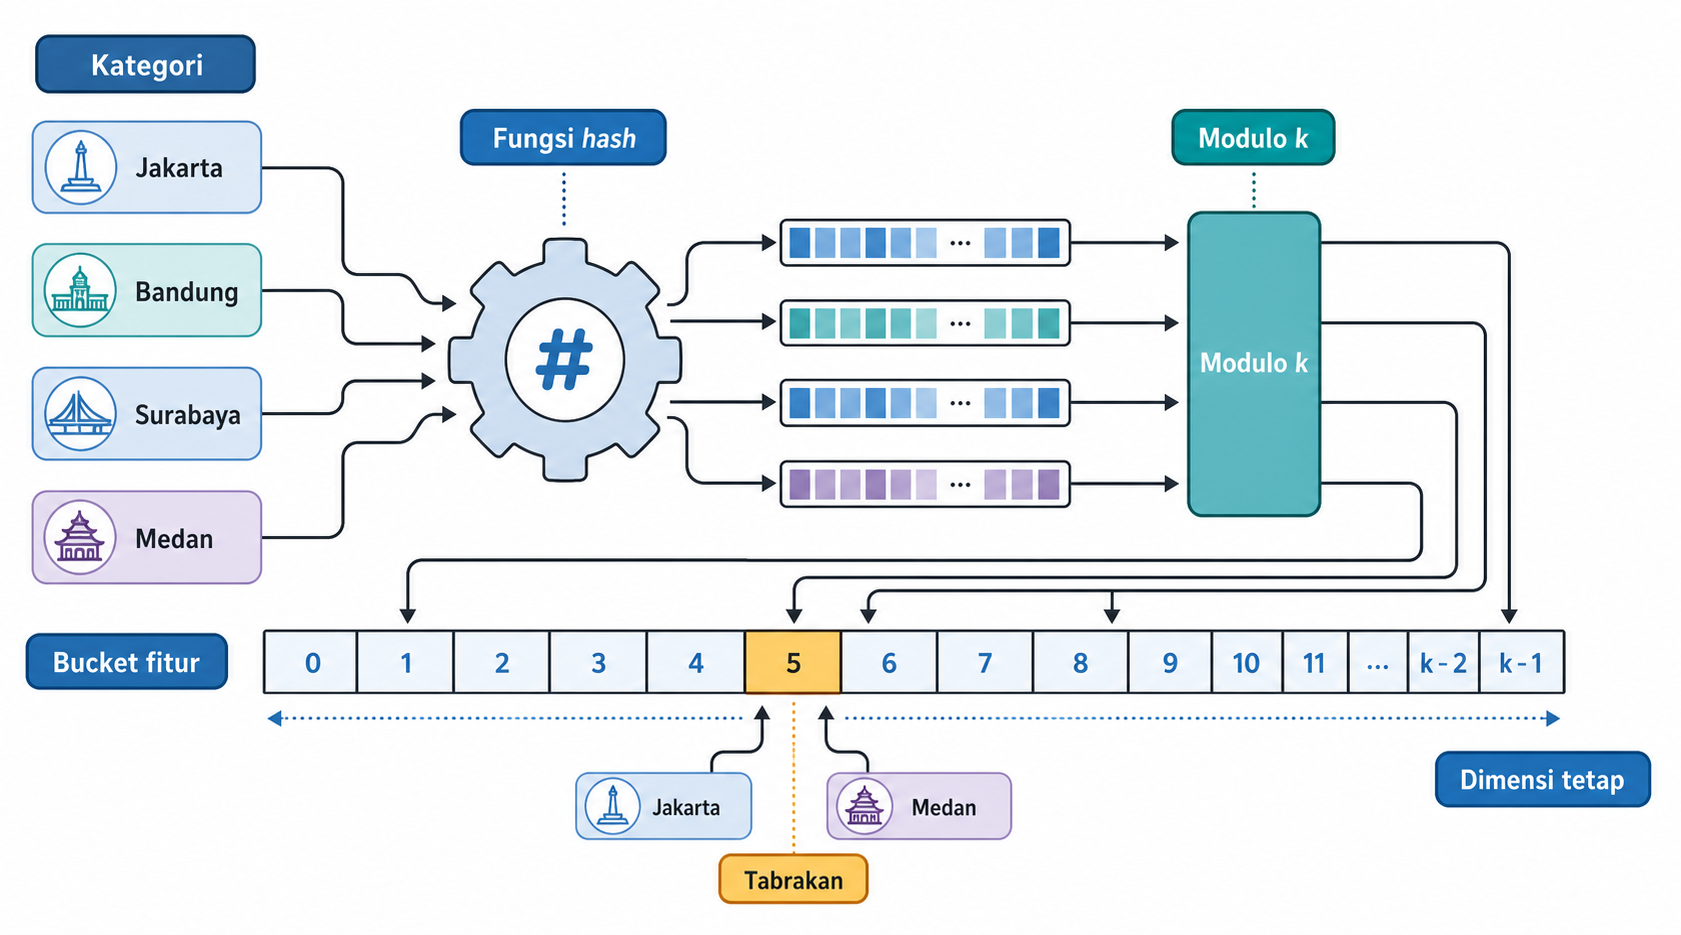
\includegraphics[width=111.6mm]{ch04-fig-3}
\caption{Hashing trick untuk kategori berkardinalitas tinggi}
\label{fig:ch04-fig-3}
\end{figure}

Hashing berguna ketika kosakata kategori tidak stabil atau terlalu besar untuk disimpan sebagai daftar eksplisit. Pendekatan ini juga memudahkan produksi karena konfigurasi yang perlu dijaga terutama adalah fungsi hash dan ukuran \(k\). Namun, interpretabilitas berkurang. Kolom hasil hashing tidak lagi memiliki arti kategori yang jelas. Dalam lingkungan yang membutuhkan audit rinci, kompromi ini perlu dipertimbangkan sebelum hashing dipilih. Jika hashing menekankan ukuran tetap, \emph{entity embedding} menekankan kedekatan antar kategori yang mirip.

\begin{pendalaman}{Meredam bias collision dengan alternate sign}
\passthrough{\lstinline!FeatureHasher!} dapat memakai tanda berbasis hash untuk memberi tanda +1 atau -1 pada kontribusi kategori. Ketika beberapa kategori bertabrakan di bucket yang sama, kontribusinya tidak selalu menumpuk searah. Sebagian dapat saling mengurangi. Dengan cara ini, \emph{noise} collision cenderung lebih netral secara harapan. Namun, alternate sign tidak menghapus collision. Pengungkit utama tetap ukuran \(k\). Menaikkan \(k\) mengurangi peluang kategori berbeda masuk ke bucket yang sama, dengan biaya memori yang lebih besar.
\end{pendalaman}

\section{\texorpdfstring{\emph{Entity Embedding}}{Entity Embedding}}\label{entity-embedding}

Hashing menjaga ukuran representasi, tetapi membuat identitas kategori bercampur ketika collision terjadi. \emph{One-hot} menjaga identitas kategori tetap terpisah, tetapi tidak menyatakan kemiripan. Dalam ruang \emph{one-hot}, Sabtu dan Minggu sama jauhnya dengan Senin dan Jumat. Padahal pada banyak tugas, akhir pekan mungkin memiliki pola target yang mirip. \emph{Entity embedding} mencoba mempelajari kemiripan seperti itu dari data.

Sebuah \emph{entity embedding} memetakan ID kategori ke vektor padat berdimensi kecil. Vektor ini dipelajari selama pelatihan model berdasarkan tujuan prediksi. Jika dua kategori membantu model dengan cara serupa, vektornya dapat bergerak berdekatan dalam ruang \emph{embedding}. Metode ini umum untuk user ID, item ID, kategori produk, lokasi, atau variabel berkardinalitas tinggi lain.

Secara konseptual, embedding lookup dapat ditulis sebagai berikut.

\[
\mathbf{e}_i = \mathbf{W}\, \mathbf{x}_i
\]

Dengan \(\mathbf{x}_i \in \{0,1\}^{|\mathcal{V}|}\) sebagai vektor \emph{one-hot} untuk kategori \(i\) dan \(\mathbf{W} \in \mathbb{R}^{d \times |\mathcal{V}|}\) sebagai matriks \emph{embedding}, hasilnya \(\mathbf{e}_i\) adalah vektor \emph{embedding} berdimensi \(d\). Dalam implementasi, operasi ini biasanya berupa lookup tabel, bukan perkalian matriks penuh.

Representasi ini berada lebih dekat ke representasi yang dipelajari mesin. Namun, keputusan manusia tetap banyak, mulai dari kolom kategori mana yang diberi \emph{embedding}, berapa dimensinya, apa tujuan pelatihannya, bagaimana validasinya, sampai bagaimana kategori langka ditangani. \emph{Embedding} dapat \emph{overfit} pada kategori jarang, dan dapat menyerap informasi sensitif atau proksi yang tidak disadari.

Gambar 4.4 memperlihatkan \emph{embedding} kategori pekerjaan atau industri. Jika dua kode pekerjaan menghasilkan pola target pendapatan yang mirip, keduanya dapat berada dekat. Inset \emph{one-hot} menunjukkan kontrasnya karena semua kategori saling berjarak sama.

\begin{figure}[tbp]\centering
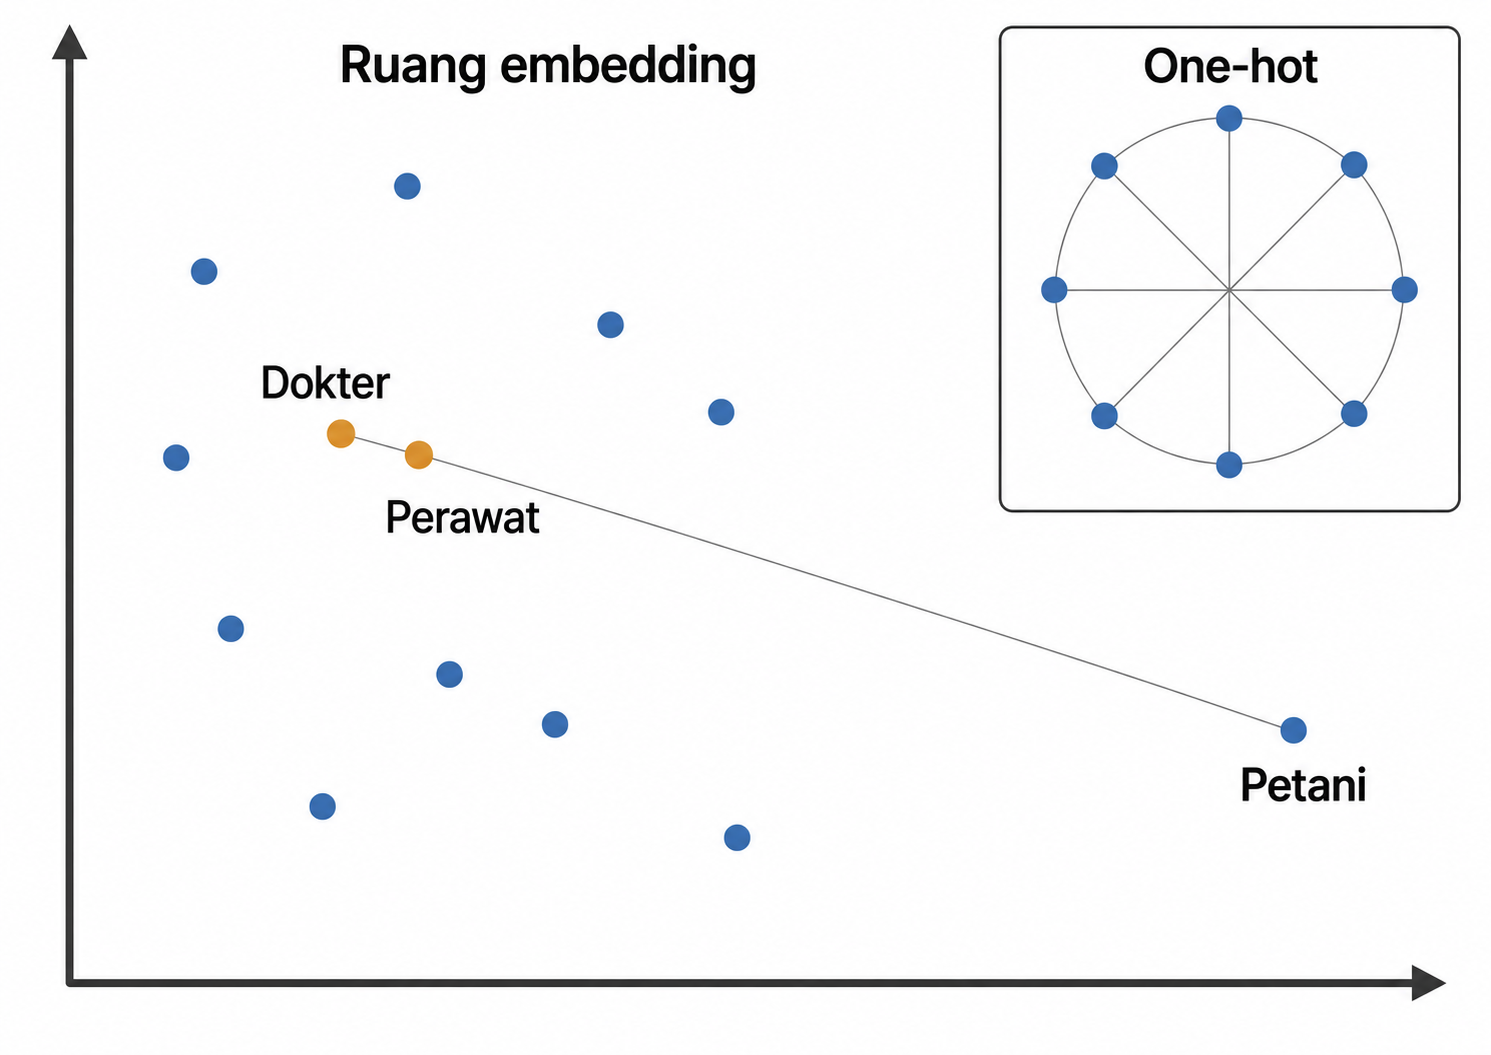
\includegraphics[width=111.6mm]{ch04-fig-4}
\caption{Ruang embedding untuk kategori}
\label{fig:ch04-fig-4}
\end{figure}

\emph{Embedding} yang sudah dilatih tidak selalu harus dipakai hanya dalam jaringan neural. Vektor \emph{embedding} dapat diekspor sebagai fitur numerik statis untuk model lain, misalnya gradient boosting. Dalam pola ini, jaringan neural dipakai sebagai pembangun fitur, sedangkan model inferensi akhir dapat berupa model non-neural. Jika \emph{embedding} dilatih secara \emph{supervised} dengan label tugas lalu diekspor, pelatihannya harus diulang di dalam setiap lipatan \emph{train} terluar atau representasi untuk model hilir harus dihasilkan secara \emph{out-of-fold}. Aturan ini berbeda dari \emph{embedding} eksternal \emph{pretrained} yang dibekukan dan tidak dilatih dengan label evaluasi tugas tersebut. Pilihan ini berguna jika \emph{embedding} memberi sinyal yang baik tetapi sistem produksi menginginkan model hilir yang berbeda. Namun, apa pun encodernya, model produksi tetap menghadapi pertanyaan yang sama tentang cara memperlakukan kategori yang belum pernah muncul saat pelatihan.

\section{Menangani Kategori Baru Saat Inferensi}\label{menangani-kategori-baru-saat-inferensi}

Semua pilihan encoding perlu menetapkan perilaku ketika kategori yang tidak ada saat pelatihan muncul setelah model dipakai. Kode wilayah dapat berubah, kategori pekerjaan dapat diperbarui, atau negara lahir yang jarang baru terlihat pada data berikutnya. Encoder yang baik bekerja pada data \emph{train} sekaligus mendefinisikan perlakuan bagi kategori yang belum pernah dilihat.

Setiap metode memiliki kebijakan sendiri. \emph{One-hot encoding} dapat menghasilkan baris \emph{all-zero} untuk kategori tak dikenal, atau mengarahkannya ke bucket kategori jarang jika bucket itu dibuat saat \emph{fit}. Dengan \passthrough{\lstinline!drop='first'!}, kode \emph{all-zero} tersebut juga mewakili kategori referensi yang dibuang, sehingga bucket eksplisit atau pemantauan diperlukan jika keduanya harus dibedakan. Ordinal encoding dapat memakai kode khusus seperti -1. Pada model pohon, kode khusus ini dapat dipisahkan dalam split tersendiri, tetapi pada model linear atau berbasis jarak tetap perlu hati-hati. Count atau frequency encoding membutuhkan nilai isian yang dikonfigurasi. \emph{Target encoding} biasanya memakai rata-rata global. Hashing menangani kategori baru secara bawaan karena string apa pun dapat di-hash. \emph{Embedding} membutuhkan indeks ``unknown'' yang memang dilatih atau diinisialisasi dengan sadar.

\emph{Rare category grouping} dapat mengurangi kerapuhan. Jika kategori yang sangat jarang digabung sejak pelatihan, model belajar perilaku bucket ``lainnya'' atau ``infrequent'' sebelum menghadapi kategori baru. Pendekatan ini memberi kebijakan yang sudah tersedia saat inferensi.

Tabel 4.1 mengembalikan seluruh bab ke sumbu keputusan yang sama. Kolom dimensi keluaran menunjukkan biaya representasi. Kolom kardinalitas membantu memilih skala masalah. Kolom kategori baru dan risiko utama perlu dibaca sebagai bagian dari desain produksi, bukan catatan tambahan. Dalam contoh Census-Income di awal bab, tabel ini membantu membedakan perlakuan untuk pendidikan, negara lahir, kode pekerjaan, dan status rumah tangga tanpa memaksa semuanya mengikuti encoder yang sama.

\tabeljudul{Tabel 4.1 — Peta keputusan encoding kategorikal}

{\def\LTcaptype{none} % do not increment counter
\par\vspace{3pt}\noindent
\begingroup\renewcommand{\arraystretch}{1.0}%
\scriptsize\linespread{1}\selectfont
\renewcommand{\_}{\textunderscore\hspace{0pt}}%
\begin{xltabular}{\linewidth}{@{}>{\raggedright\arraybackslash}p{(\linewidth-8\tabcolsep)*\real{0.140}} >{\raggedright\arraybackslash}p{(\linewidth-8\tabcolsep)*\real{0.138}} >{\raggedright\arraybackslash}p{(\linewidth-8\tabcolsep)*\real{0.160}} >{\raggedright\arraybackslash}p{(\linewidth-8\tabcolsep)*\real{0.197}} >{\raggedright\arraybackslash}p{(\linewidth-8\tabcolsep)*\real{0.365}}@{}}
\toprule

Metode
 & 
Dimensi keluaran
 & 
Kardinalitas
 & 
Kategori baru
 & 
Risiko utama
 \\
\midrule
\endhead




\emph{One-hot} & \(|\mathcal{V}|\) kolom biner & Rendah-menengah & \emph{All-zero} \slash{} infrequent bucket & Ledakan dimensi dan \emph{sparsity}. Unknown dapat menyatu dengan referensi yang di-\emph{drop} \\
Ordinal & 1 kolom numerik & Rendah, ordinal sejati & Kode khusus, misalnya -1 & Urutan palsu di model linear\slash{}jarak \\
Count\slash{}Frequency & 1 kolom numerik & Tinggi & Nilai isian terkonfigurasi & Tabrakan nilai, bukan makna semantik \\
\emph{Target encoding} & 1 kolom numerik & Tinggi & Rata-rata global & \emph{Target leakage} tanpa cross-fitting \\
Hashing & \(k\) kolom tetap & Sangat tinggi \slash{} tak terbatas & Otomatis by construction & Collision dan hilang interpretabilitas \\
\emph{Entity embedding} & \(d\) kolom padat & Tinggi & Indeks unknown terlatih & \emph{Overfit} kategori langka, butuh data dan komputasi \\
\bottomrule
\end{xltabular}\endgroup\par\vspace{5pt}

}

Perilaku kategori baru sebaiknya diuji dengan sengaja. Jangan mengandalkan data \emph{test} yang kebetulan hanya berisi kategori yang sudah dikenal. Dalam produksi, distribusi kategori dapat bergeser. Memantau jumlah kategori baru, kategori jarang, dan perubahan frekuensi kategori adalah bagian dari menjaga kualitas fitur.

\begin{sintesis}

Pengodean kategorikal adalah keputusan representasi, bukan sekadar pekerjaan mengubah label menjadi angka. Nominal, ordinal, biner, dan kategori berkardinalitas tinggi memerlukan perlakuan yang berbeda karena maknanya berbeda. Encoder yang baik mempertahankan makna yang dibutuhkan model, mengendalikan dimensi keluaran, memiliki perilaku jelas untuk kategori baru, dan tidak merusak validasi. Tabel 4.1 dapat dipakai sebagai peta keputusan ringkas ketika satu \emph{dataset} memuat beberapa jenis kategori sekaligus.

\emph{One-hot encoding} aman untuk kategori nominal dengan kardinalitas rendah sampai menengah, tetapi dapat membuat matriks sangat lebar. Ordinal encoding hemat, tetapi hanya wajar ketika urutan memang bermakna atau model dapat menoleransi kode arbitrer. Count dan frequency encoding mengompresi kategori banyak, tetapi kehilangan identitas semantik. \emph{Target encoding} kuat tetapi berisiko \emph{leakage}. Hashing cocok untuk kategori tak terbatas dengan harga collision dan interpretabilitas. \emph{Embedding} belajar kemiripan kategori, tetapi membutuhkan data, validasi, dan pengendalian \emph{overfit}.

Keputusan encoding juga perlu mempertimbangkan \emph{pipeline}, kategori baru, \emph{rare category}, interpretabilitas, dan keluarga model yang akan memakai fitur. Dengan pertimbangan tersebut, kategori dapat diubah menjadi representasi yang sesuai dengan makna dan risiko pemodelannya.

\end{sintesis}

\begin{bacaan}

\begin{itemize}
\tightlist
\item
  scikit-learn --- Comparing Target Encoder --- \url{https://scikit-learn.org/stable/auto_examples/preprocessing/plot_target_encoder.html}. Perbandingan target encoding dengan encoder lain.
\item
  scikit-learn --- Target Encoder Internal Cross Fitting --- \url{https://scikit-learn.org/stable/auto_examples/preprocessing/plot_target_encoder_cross_val.html}. Mengapa cross-fitting mencegah kebocoran target.
\item
  Guo \& Berkhahn (2016), Entity Embeddings --- \url{https://arxiv.org/abs/1604.06737}. Embedding kategori dari jaringan neural.
\item
  Prokhorenkova dkk. (2018), CatBoost --- \url{https://arxiv.org/abs/1706.09516}. Ordered target statistics untuk kategori.
\item
  Feature-engine --- Categorical encoding --- \url{https://feature-engine.trainindata.com/en/latest/api_doc/encoding/index.html}. Count/frequency dan rare-label encoder.
\item
  Weinberger dkk. (2009), Feature Hashing (ICML) --- \url{https://arxiv.org/abs/0902.2206}. Hashing trick untuk kardinalitas sangat tinggi.
\end{itemize}

\end{bacaan}

\rujukanheading

\protect\phantomsection\label{refs}
\begin{CSLReferences}{1}{1}
\bibitem[\citeproctext]{ref-miccibarreca2001}
Micci-Barreca, Daniele. 2001. {``A Preprocessing Scheme for High-Cardinality Categorical Attributes in Classification and Prediction Problems.''} \emph{ACM SIGKDD Explorations Newsletter} 3 (1): 27--32.

\end{CSLReferences}

% ==========================================================================
% ch05.tex — dihasilkan otomatis dari website/chapters/ch05.qmd
% Boleh disunting manual. 'sync' hanya menimpa bila .qmd berubah DAN .tex
% belum disunting; kalau keduanya berubah, dilewati (pakai --force).
% qmd-sha1: fb804da995a7
% tex-sha1: 846582b624be
% ==========================================================================
% >>>>> ISI OTOMATIS (jangan hapus baris ini) >>>>>
\chapter{Missing Values \& Outliers (Reproducible, Berbasis Pipeline)}\label{missing-values-outliers-reproducible-berbasis-pipeline}

Ketiadaan data dan kehadiran \emph{outlier} merupakan kenyataan empiris yang senantiasa dijumpai saat bekerja dengan data mentah di dunia nyata. Algoritma pemelajaran mesin tidak dapat memproses nilai kosong pada saat kalkulasi gradien atau metrik jarak, sedangkan \emph{outlier} ekstrem yang menyimpang jauh dari pusat distribusi dapat mendistorsi estimasi parameter model. Sayangnya, tindakan pembersihan data baris per baris di luar alur sistematis sering kali mengubah variansi asli, menyembunyikan anomali yang valid, dan memicu \emph{data leakage} jika parameter pengisi dihitung sebelum pemisahan data (\emph{data split}) dilakukan.

Bab ini mendeskripsikan fondasi penanganan nilai kosong dan \emph{outlier} secara sistematis, \emph{reproducible}, dan terintegrasi di dalam objek \emph{pipeline}. Pembahasan mencakup mekanisme hilangnya data (MCAR, MAR, MNAR) sebagai asupan diagnostik sebelum otomatisasi, pemilihan imputasi sederhana melawan imputasi iteratif multivariat berbasis model, pemanfaatan status kekosongan sebagai \emph{feature} representatif (\emph{missing indicator}), serta transformasi \emph{outlier} menggunakan parameter statistik yang tangguh (\emph{robust}). Seluruh proses ini dikemas ke dalam alur kerja terstruktur untuk menjamin integritas distribusi data dari tahap pelatihan hingga fase inferensi di lingkungan produksi.

\section{\texorpdfstring{\emph{Missing Values} \& \emph{Outlier} (Reproducible, Berbasis \emph{pipeline})}{Missing Values \& Outlier (Reproducible, Berbasis pipeline)}}\label{missing-values-outlier-reproducible-berbasis-pipeline}

\textbf{Mekanisme \emph{Missingness}: MCAR, MAR, dan MNAR.}\label{mekanisme-missingness-mcar-mar-dan-mnar}

Sebagian besar algoritma \emph{machine learning} tidak dapat memproses nilai kosong secara langsung, sehingga data yang tidak lengkap harus disesuaikan sebelum tahap pemodelan. Sebelum menyusun strategi imputasi di dalam \emph{pipeline}, alasan di balik hilangnya data tersebut perlu diinspeksi. Ketiadaan nilai sering kali merepresentasikan kejadian faktual yang membawa informasi spesifik tentang prosedur perekaman observasi. Tahap diagnostik ini sangat penting sebelum menerapkan transformasi otomatis.

Secara matematis, mekanisme hilangnya data (\emph{missingness mechanism}) didefinisikan melalui probabilitas bersyarat dari matriks indikator kekosongan. Misalkan terdapat sekumpulan data \(Y\) yang terdiri dari bagian teramati \(Y_{obs}\) dan bagian kosong \(Y_{miss}\). Jika kita mendefinisikan matriks indikator \(R\) dengan nilai 1 berarti data hilang dan 0 berarti teramati, mekanisme \emph{missingness} dinyatakan sebagai fungsi probabilitas \(P(R \mid Y_{obs}, Y_{miss}, \phi)\). Dalam fungsi tersebut, \(R\) merepresentasikan matriks indikator ketiadaan data, \(Y_{obs}\) adalah nilai atribut yang berhasil terekam, \(Y_{miss}\) adalah nilai atribut yang kosong, dan \(\phi\) merupakan parameter tidak diketahui yang menentukan proses hilangnya data. Berdasarkan hubungan ketergantungan ini, statistika membagi hilangnya data ke dalam tiga kategori utama.

Kategori pertama adalah \emph{Missing Completely At Random} (MCAR). Pada kasus ini, kekosongan terjadi murni secara kebetulan dan peluang hilangnya data tidak dipengaruhi oleh variabel lain. Bentuk distribusinya disederhanakan menjadi \(P(R \mid Y_{obs}, Y_{miss}, \phi) = P(R \mid \phi)\). Contohnya, sensor pengukur angin gagal mengirimkan data sesaat akibat pemadaman listrik acak. Pada skenario MCAR, porsi data yang utuh tetap menjadi sampel representatif dari populasi awal.

Kategori kedua adalah \emph{Missing At Random} (MAR). Peluang terjadinya nilai kosong memiliki probabilitas bersyarat dengan variabel lain di dalam \emph{dataset}, tetapi tidak dipengaruhi oleh nilai atribut yang hilang itu sendiri. Persamaannya diukur menjadi \(P(R \mid Y_{obs}, Y_{miss}, \phi) = P(R \mid Y_{obs}, \phi)\). Sebagai contoh, responden survei berusia lanjut sering mengosongkan riwayat aktivitas fisik. Pola kekosongan pada riwayat olahraga tersebut pada dasarnya berkorelasi matematis dengan rentang usia responden. Memisahkan pengamatan berdasarkan umur akan menghasilkan probabilitas kekosongan yang independen pada setiap kelompok batas usianya.

Kategori ketiga adalah \emph{Missing Not At Random} (MNAR). Probabilitas hilangnya suatu nilai terikat langsung dengan isi dari nilai yang tidak teramati tersebut (\(Y_{miss}\)). Ketergantungan ini membuat persamaan probabilitas tidak dapat disederhanakan. Kasus klasiknya adalah survei pendapatan, di mana responden dengan angka kekayaan ekstrem sering kali menolak melapor demi privasi. Absennya data merupakan dampak langsung dari nominal kekayaan itu sendiri, sehingga pada kondisi MNAR, lokasi kekosongan justru mengandung sinyal pemodelan yang kuat.

\begin{figure}[htbp]\centering
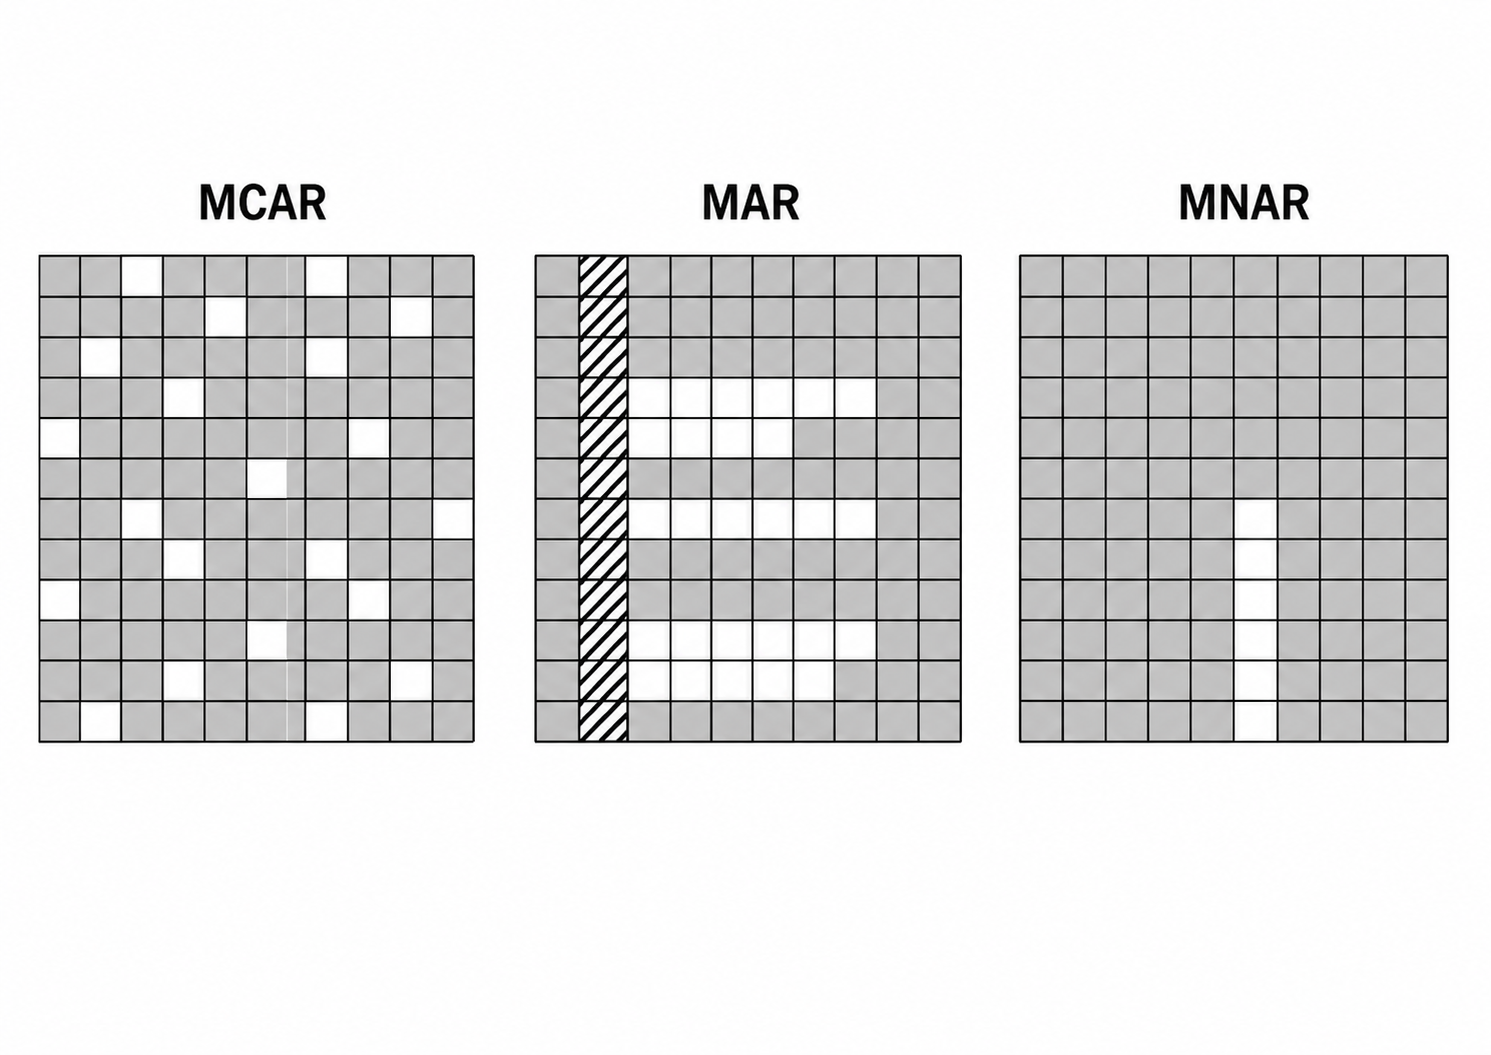
\includegraphics[width=\linewidth,height=0.72\textheight,keepaspectratio]{ch05-fig-1}
\caption{Perbandingan Pola Hilangnya Data pada Mekanisme MCAR, MAR, dan MNAR}
\label{fig:ch05-fig-1}
\end{figure}

Membedakan ketiga profil mekanisme di atas mencegah injeksi bias pada fase pelatihan. Jika kita mengisi data yang tergolong MNAR menggunakan nilai rata-rata, kita akan mendistorsi batas distribusi asli dan menyamarkan keberadaan kelompok ekstrem dalam sampel.

Penerapan fungsi pengamatan statistik memfasilitasi proses inspeksi ini. Pengujian berbasis validasi observasional ini dapat dicapai melalui visualisasi matriks kekosongan yang direpresentasikan oleh fungsi pustaka \passthrough{\lstinline!missingno!}. Korelasi kosong (\emph{nullity}) komparatif di antara dua lajur parameter menandakan kehadiran relasi struktural bertipe MAR maupun MNAR. Pada evaluasi formal, uji statistik MCAR Little dioperasikan untuk meninjau secara mekanis rasio asumsi deviasi \emph{missingness}. Meskipun indikasi matematis memberikan acuan awal, pendekatan kuantitatif ini harus diverifikasi berdampingan dengan evaluasi konteks domain faktual data terkait. Jika kondisi absen bertipe MNAR teridentifikasi, parameter kosong tersebut berfungsi menjadi sinyal observasi mandiri. Beberapa arsitektur \emph{deep learning} di desain khusus memetakan nilai kosong (\emph{missing value}) sebagai bagian indikator mekanisme pemelajaran internal untuk menyelaraskan akurasi prediksi asimetris.

Operasi imputasi \emph{missing values} memerlukan pendekatan yang sistematis. Pemahaman konseptual, inspeksi visual, serta pengetahuan konteks domain merupakan prasyarat mutlak sebelum mengubah teknik penanganan nilai kosong menjadi komponen \emph{pipeline} permanen.

\section{\texorpdfstring{Imputasi Sebagai Komponen \emph{Pipeline}}{Imputasi Sebagai Komponen Pipeline}}\label{imputasi-sebagai-komponen-pipeline}

Praktik yang sering keliru dalam pengembangan model adalah memposisikan penanganan data kosong sebagai tahap pembersihan di awal proses. Data diisi menggunakan rata-rata atau median dari keseluruhan \emph{dataset}, baru kemudian dibagi menjadi \emph{split training} dan \emph{split test}. Pendekatan ini memicu \emph{data leakage} karena tahap imputasi tidak terisolasi dari data uji. Imputasi adalah transformasi struktural yang harus tertanam di dalam \emph{pipeline} pemodelan.

Fenomena \emph{data leakage} terjadi karena perhitungan statistik merekam informasi dari kelompok evaluasi. Jika sekumpulan data \(X\) merupakan gabungan data latih dan data uji, persamaan rata-rata imputasi yang terdistorsi adalah:

\[ \mu_{bocor} = \frac{1}{|X_{train}| + |X_{test}|} \left( \sum_{x \in X_{train}} x + \sum_{x \in X_{test}} x \right) \]

Suku \(\sum_{x \in X_{test}} x\) memastikan bahwa parameter pengisi pada data latih dihitung dengan menyertakan komponen distribusi uji. Akibatnya, model menyesuaikan fungsi internalnya berdasarkan rentang angka observasi masa depan yang direpresentasikan saat sesi inisialisasi pelatihan. Hasilnya, metrik kalkulasi skor tampak sangat akurat pada data eksperimental, namun akan mengalami tingkat kesalahan klasifikasi yang signifikan saat diaplikasikan pada baris \emph{dataset} di operasional lingkungan \emph{production}.

\begin{figure}[htbp]\centering
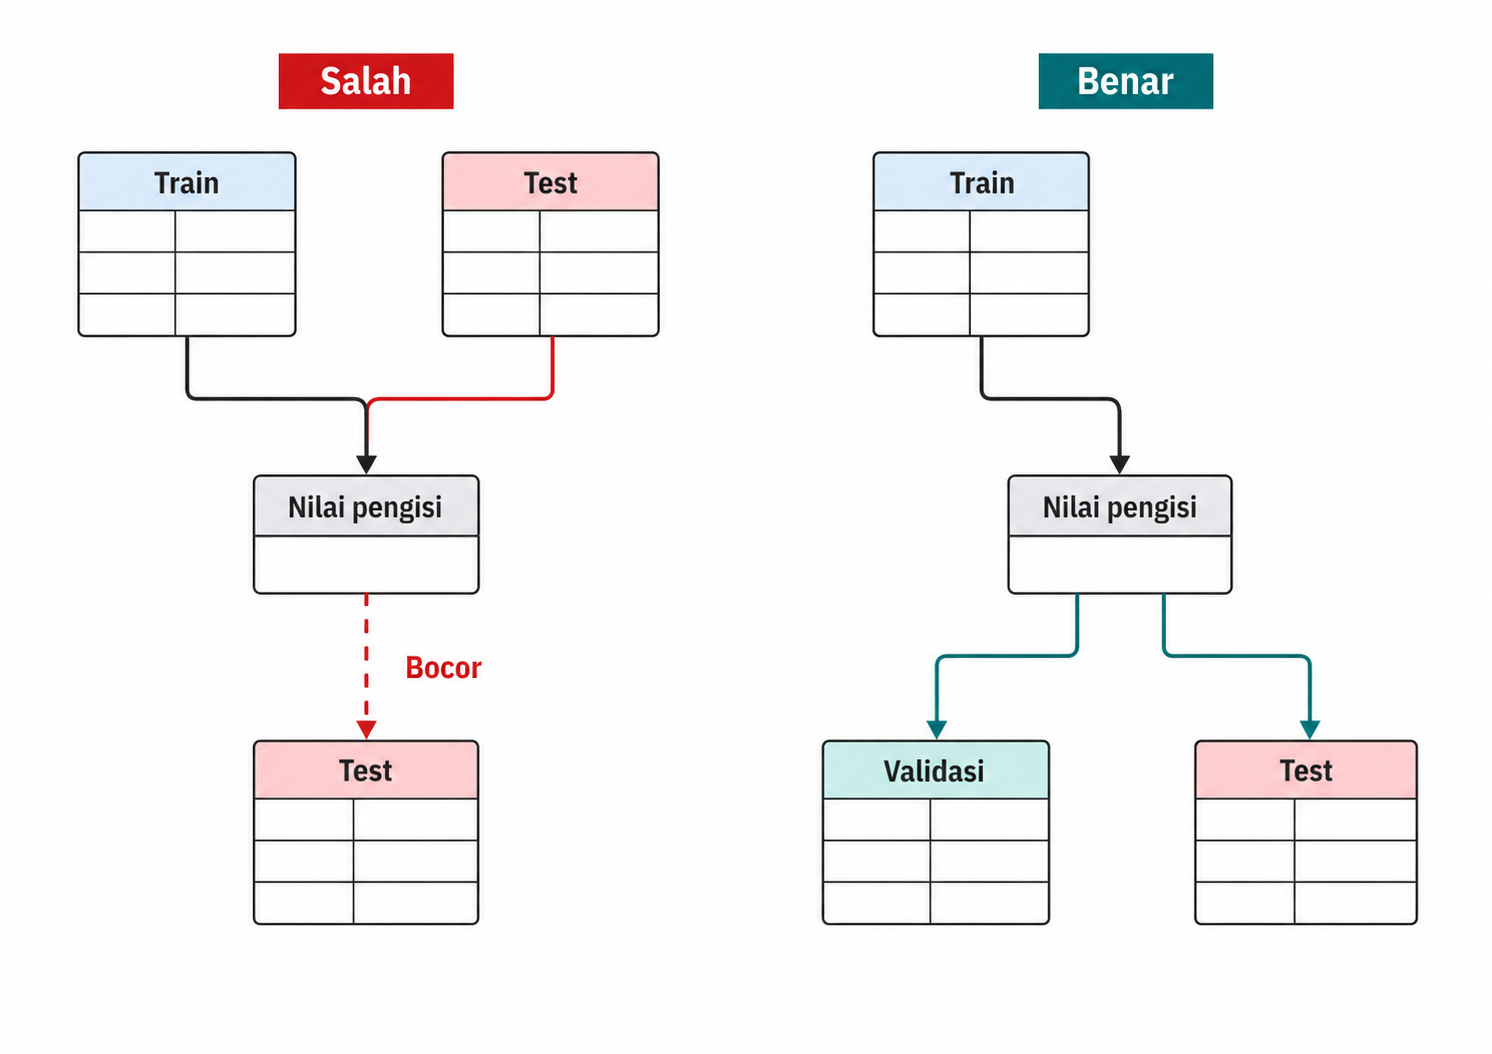
\includegraphics[width=\linewidth,height=0.72\textheight,keepaspectratio]{ch05-fig-2}
\caption{Alur Imputasi Data Utuh yang Menyebabkan Kebocoran}
\label{fig:ch05-fig-2}
\end{figure}

\begin{figure}[htbp]\centering
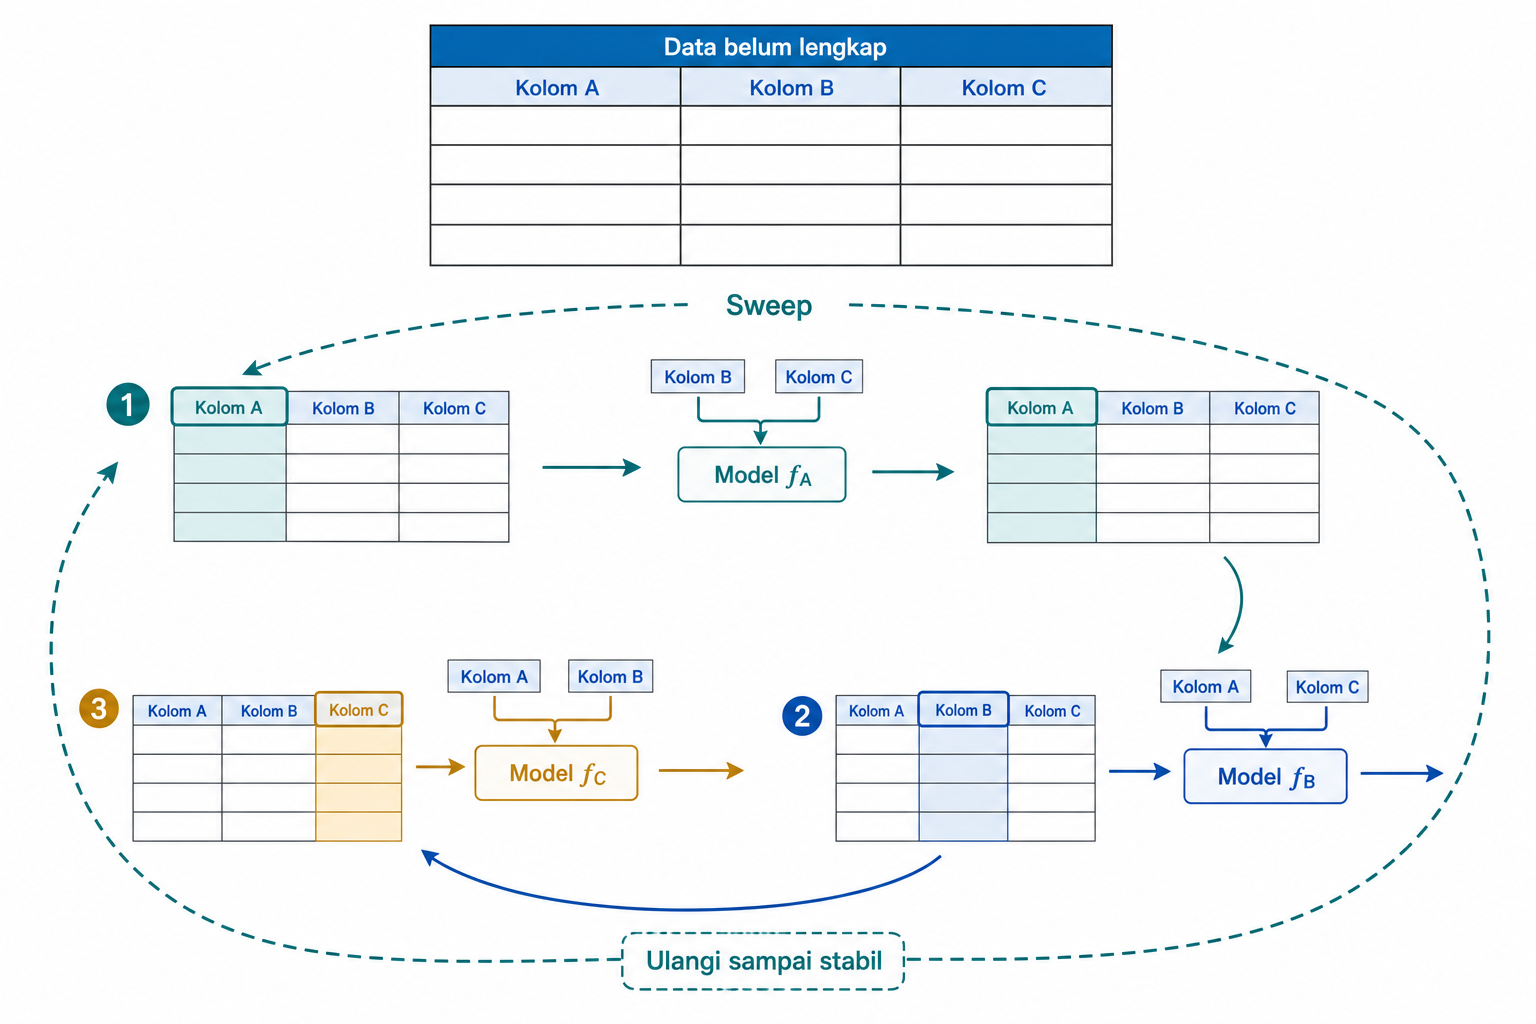
\includegraphics[width=\linewidth,height=0.72\textheight,keepaspectratio]{ch05-fig-3}
\caption{Alur Imputasi Aman Menggunakan Pipeline}
\label{fig:ch05-fig-3}
\end{figure}

Untuk menghindari \emph{data leakage}, modul imputasi (seperti \passthrough{\lstinline!SimpleImputer!} atau \passthrough{\lstinline!KNNImputer!} pada pustaka Scikit-Learn) harus diperlakukan sama seperti model prediktif, melalui pemisahan fase \emph{fit} dan \emph{transform}. Nilai pengisi dihitung eksklusif dari \emph{split training}:

\[ \mu_{benar} = \frac{1}{|X_{train}|} \sum_{x \in X_{train}} x \]

Siklus fungsi arsitektur dari parameter indikasi imputasi ini memaksa evaluasi statistik untuk dikerjakan independen. Pertama, kerangka kerja terisolasi berimplikasi pada fungsi komputasi \emph{cross-validation}. Parameter nilai estimasi diformulasikan ulang pada blok data terpisah pelatihan (\emph{fold}), menghindarkan tumpukan lipatan kelompok uji (\emph{validation fold}) dari kebocoran sinyal referensi perhitungan parameter aslinya. Kedua, kerangka operasional imputasi yang konsisten meniadakan kendala komputasi pada fungsional algoritma di tingkat operasional *production*. Varians observasi tabel asing yang didatangkan untuk dievaluasi oleh parameter metode prediktif secara fungsional dinilai hanya merujuk acuan distribusi pelatihan yang sebelumnya disematkan oleh modul imputer bawaan. Ketiga, prosedur penyisipan yang memusat meredam distorsi komputasi untuk mekanisme multivariat interaktif. Algoritma seperti prediksi klasifikasi antar kolom \emph{features} diharuskan berjalan independen memanfaatkan murni \emph{split training} observasinya.

Meskipun beberapa kajian literatur menyimpulkan bahwa imputasi median tak-diawasi (*unsupervised*) yang tidak beroperasi melalui isolasi \emph{cross-validation} sesekali memperkecil perhitungan tingkat ukuran varians dengan membebankan penalti fungsional parameter metrik observasi pada ukuran parameter bias (Jaeger dkk., 2020), standar mutlak prapemrosesan harus dijaga. Penggabungan logika algoritma imputer dikerjakan konsisten hanya sesudah fungsi isolasi prapemrosesan rentang pemisahan *split* parameter observasi diterapkan sebagai komponen terpadu variabel *transformer* pada urutan parameter komputasi \emph{pipeline}.

\section{Imputasi Sederhana vs.~Berbasis Model}\label{imputasi-sederhana-vs.-berbasis-model}

Pemilihan algoritma pengisian nilai kosong bergantung pada mekanisme \emph{missingness} (MCAR, MAR, atau MNAR). Pendekatan imputasi terbagi ke dalam dua metode: metode univariat dasar yang memprioritaskan kecepatan kalkulasi dan metode multivariat yang berusaha mempertahankan struktur distribusi data asli.

\textbf{Imputasi Univariat (Sederhana).}\label{imputasi-univariat-sederhana}

Imputasi sederhana mengisi sel data kosong menggunakan metrik statistik tunggal dari kolom yang sama, seperti rata-rata (\emph{mean}), median, atau modus.

Karakteristik metode pendekatan imputasi komputasi univariat didasarkan murni pada tingkat kemudahan komputasi algoritma pemrosesannya. Kalkulasi matematis bekerja dengan singkat dengan menyajikan evaluasi fungsi linear sekuensial. Tetapi, kelebihan tersebut hadir mengabaikan fungsi analisis silang (\emph{cross-correlation}) karena setiap variabel kolom beroperasi mutlak secara independen. Misalnya jika rentang dimensi parameter berat badan dinormalisasi berbasis indeks median global distribusi dari *dataset*, kalkulasi estimasi angka yang hilang tersebut tidak dipandu rujukan data variabel fungsional kelompok umur maupun proporsi dimensi ukuran tinggi secara spesifik dari sampel baris pengamatan itu. Imputasi angka titik berpusat juga berdampak signifikan dengan menekan simpangan angka (\emph{variance shrinkage}) data tersebut. Konsentrasi jumlah titik yang sama pada garis median secara proporsional menekan pelebaran sebaran data populasi awal. Rekayasa parameter nilai varians mendistorsi rasio perbandingan galat dimensi matematis (\emph{standard error}) ketika \emph{machine learning} melacak konvergensi prediksi komputasi titik sasarannya.

\textbf{Imputasi Multivariat (Berbasis Model).}\label{imputasi-multivariat-berbasis-model}

Untuk mempertahankan korelasi struktural antar-\emph{feature}, imputasi multivariat memperlakukan kolom berstatus \emph{missing} sebagai variabel target prediksi, sementara lajur kolom utuh difungsikan secara bergantian sebagai matriks penjelas.

Dua algoritma klasik utama di kelas multivariat ini adalah K-Nearest Neighbors (KNN) dan Imputasi Iteratif (MICE). Algoritma KNN mengisi sel renggang melalui rata-rata nilai dari gabungan tetangga terdekatnya. Proses pencariannya mengeksekusi parameter jarak spesifik hanya dari rentang variabel yang bebas sel kosong. Di sisi lain, \emph{Multiple Imputation by Chained Equations} (MICE) menyusun rantai prediksi dengan melatih fungsi regresi pada tiap-tiap target kolom secara berurutan dalam skema \emph{round-robin}.

\begin{figure}[htbp]\centering
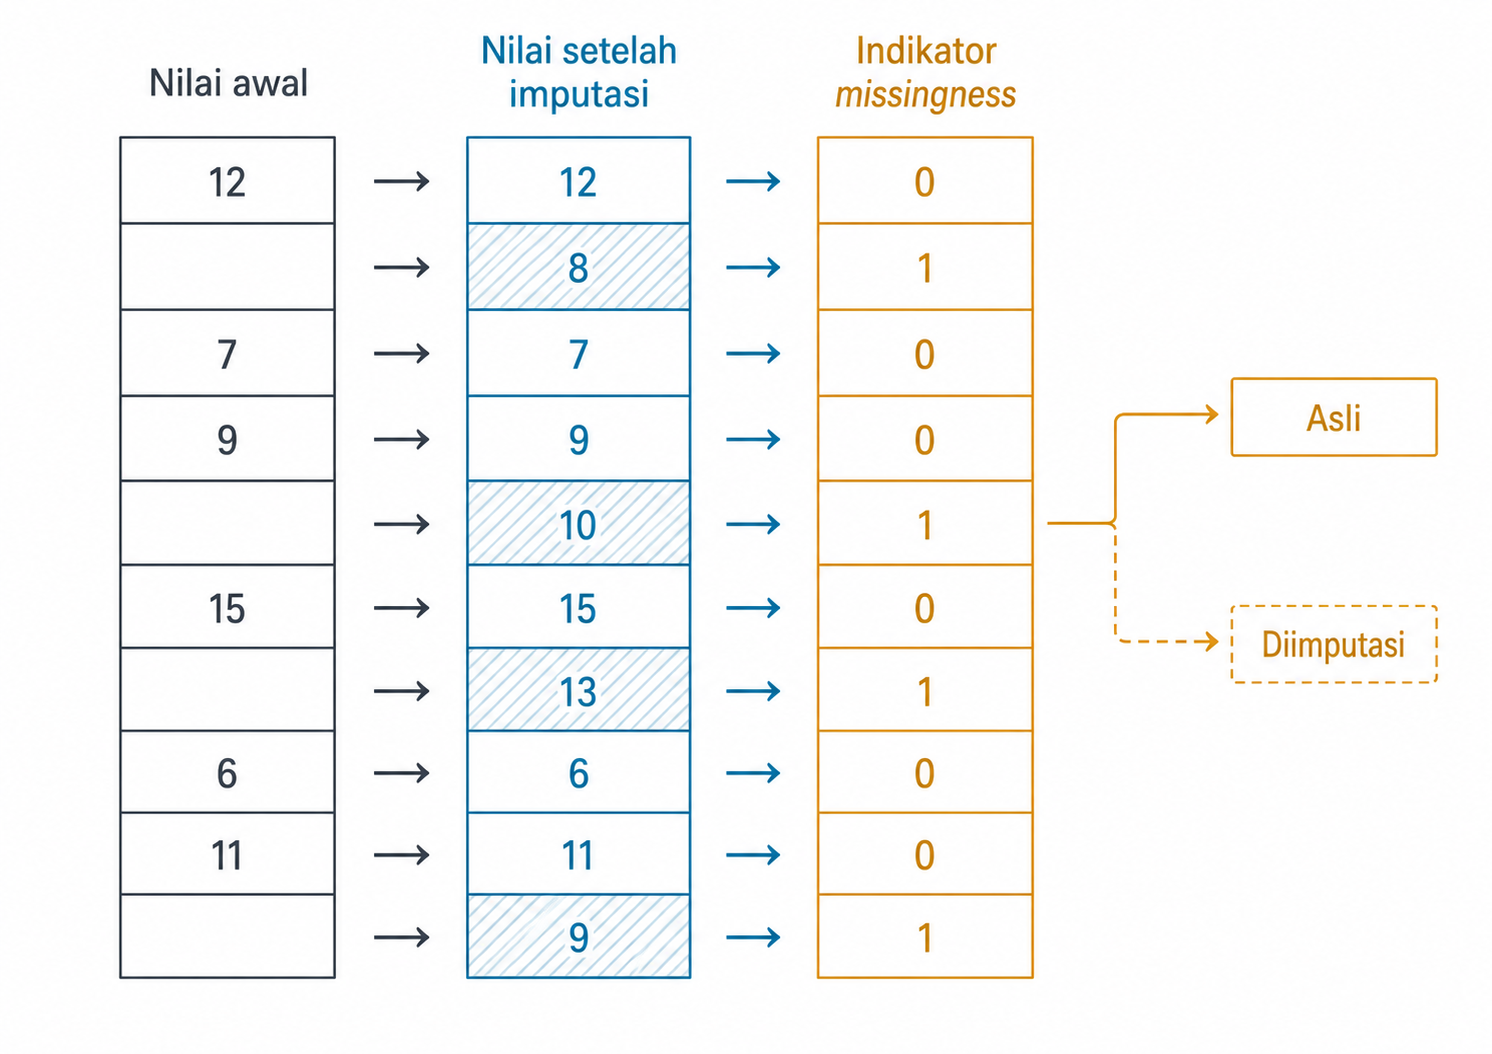
\includegraphics[width=\linewidth,height=0.72\textheight,keepaspectratio]{ch05-fig-4}
\caption{Siklus Prediksi Berantai pada Algoritma MICE}
\label{fig:ch05-fig-4}
\end{figure}

Secara matematis, prediksi fungsi target pada skema imputasi iteratif dikalkulasikan dengan formula \(\hat{x}_{i,j}^{(t)} = f_j \left( x_{i,1}^{(t)}, \dots, x_{i,j-1}^{(t)}, x_{i,j+1}^{(t-1)}, \dots, x_{i,p}^{(t-1)} \right)\). Dalam persamaan tersebut, \(\hat{x}_{i,j}^{(t)}\) menyatakan angka proyeksi pada sel baris ke-\(i\) di kolom \(j\) untuk siklus ke-\(t\). Variabel \(f_j\) mewakili algoritma pemelajaran mesin tersupervisi (contohnya \emph{Random Forest} atau regresi) yang ditugaskan khusus membedah varians kolom \(j\). Model ini mencerna deret data secara kontinu: meminjam pembaruan nilai kelompok indeks \(1\) sampai \(j-1\) dari iterasi terkini \((t)\), lalu memanfaatkan sisa rentang dari \(j+1\) hingga dimensi puncak \(p\) dari siklus masa lalu \((t-1)\). Modul arsitektur pustaka modern seperti \passthrough{\lstinline!IterativeImputer!} umumnya dikonfigurasi untuk memberikan prediksi nilai tunggal (\emph{single imputation}) demi mereduksi kerumitan \emph{pipeline} komputasi inferensi, walau hal ini menghilangkan visibilitas atas ketidakpastian angka penambalan (\emph{imputation uncertainty}) yang biasanya dikelola lewat metodologi MICE murni.

\textbf{Pendekatan Generatif Berbasis Deep Learning.}\label{pendekatan-generatif-berbasis-deep-learning}

Pada saat matriks \emph{feature} berkembang menjadi dimensi raksasa yang mengandung distribusi dependensi tak-linear, perhitungan \emph{deep learning} menghasilkan variasi penyelesaian komputasi imputasi fungsional tersupervisi. Sebagai gambaran struktural, model jaringan \emph{Masked Autoencoder} mengubah parameter kekosongan pengamatan menjadi segmen lapisan (\emph{mask}) untuk menstimulasi fungsi pengenalan mandiri \emph{self-supervised} dalam menalar sebaran rasio varians asli pada data berdimensi utuh. Pada model *diffusion* probabilistik (\emph{Diffusion Models}), pergeseran matematis metode penyebaran transmisi *noise* diadaptasi untuk menghitung kemungkinan pengisian nilai \emph{feature} dengan pendekatan estimasi yang menyerupai fungsi *baseline* rasio asli data. Modifikasi desain untuk jaringan deteksi pola MNAR (seperti fungsional model \passthrough{\lstinline!not-MIWAE!}) melepaskan belenggu probabilitas matematis dari sistem acak (MAR) pada skema evaluasi *training* konvensional. Model arsitektur ini memetakan observasi parameter \emph{missingness} sebagai mekanisme terintegrasi ke dalam rancangan pembobotan prediksi matriks observasi fungsional multi-layer.

Dominasi tingkat performa arsitektur jaringan generasi baru ini hampir selalu menuntut biaya komputasi yang tinggi. Banyak pakar komparatif metrik modern, direpresentasikan dalam dokumen analisis Näf (2026), merekomendasikan komputasi fungsional imputasi stokastik berbantuan regresi pohon berjejer (\emph{MICE-Random Forest}) lantaran margin selisih kapabilitas prediksinya kerap kali sangat tipis dibandingkan model generatif yang kompleks. Keberhasilan parameter probabilitas klasik menjustifikasi fungsinya baik sebagai \emph{baseline} fungsional maupun parameter penyeimbang pada optimisasi utilitas ruang arsitektur generatif modern.

\section{\texorpdfstring{\emph{Missing Indicator} Sebagai Sinyal}{Missing Indicator Sebagai Sinyal}}\label{missing-indicator-sebagai-sinyal}

Ketika berhadapan dengan data yang tidak lengkap, proses imputasi secara otomatis menghapus sebuah informasi struktural: fakta bahwa observasi tersebut awalnya kosong. Ketidakhadiran sebuah nilai sering kali menyimpan sinyal prediktif yang lebih kuat daripada nilai tebakan yang dimasukkan oleh algoritma imputasi.

Untuk mempertahankan informasi ini, kita mengonstruksi \emph{feature} biner tambahan yang disebut \emph{missing indicator}. \emph{Feature} ini memisahkan operasi pengisian nilai dari status ketersediaan data awal. Secara matematis, untuk sebuah \emph{feature} \(x^{(j)}\), indikator \(m^{(j)}\) didefinisikan melalui persamaan berikut:

\[
m_i^{(j)} = \begin{cases}
1, & \text{jika } x_i^{(j)} \text{ bernilai NaN (kosong)} \\
0, & \text{jika } x_i^{(j)} \text{ terobservasi}
\end{cases}
\]

Dalam rumusan ini, variabel \(m_i^{(j)}\) mewakili elemen indikator biner untuk observasi ke-\(i\) pada \emph{feature} ke-\(j\), sedangkan \(x_i^{(j)}\) merepresentasikan nilai asli dari data sebelum melewati tahapan imputasi.

\begin{figure}[htbp]\centering
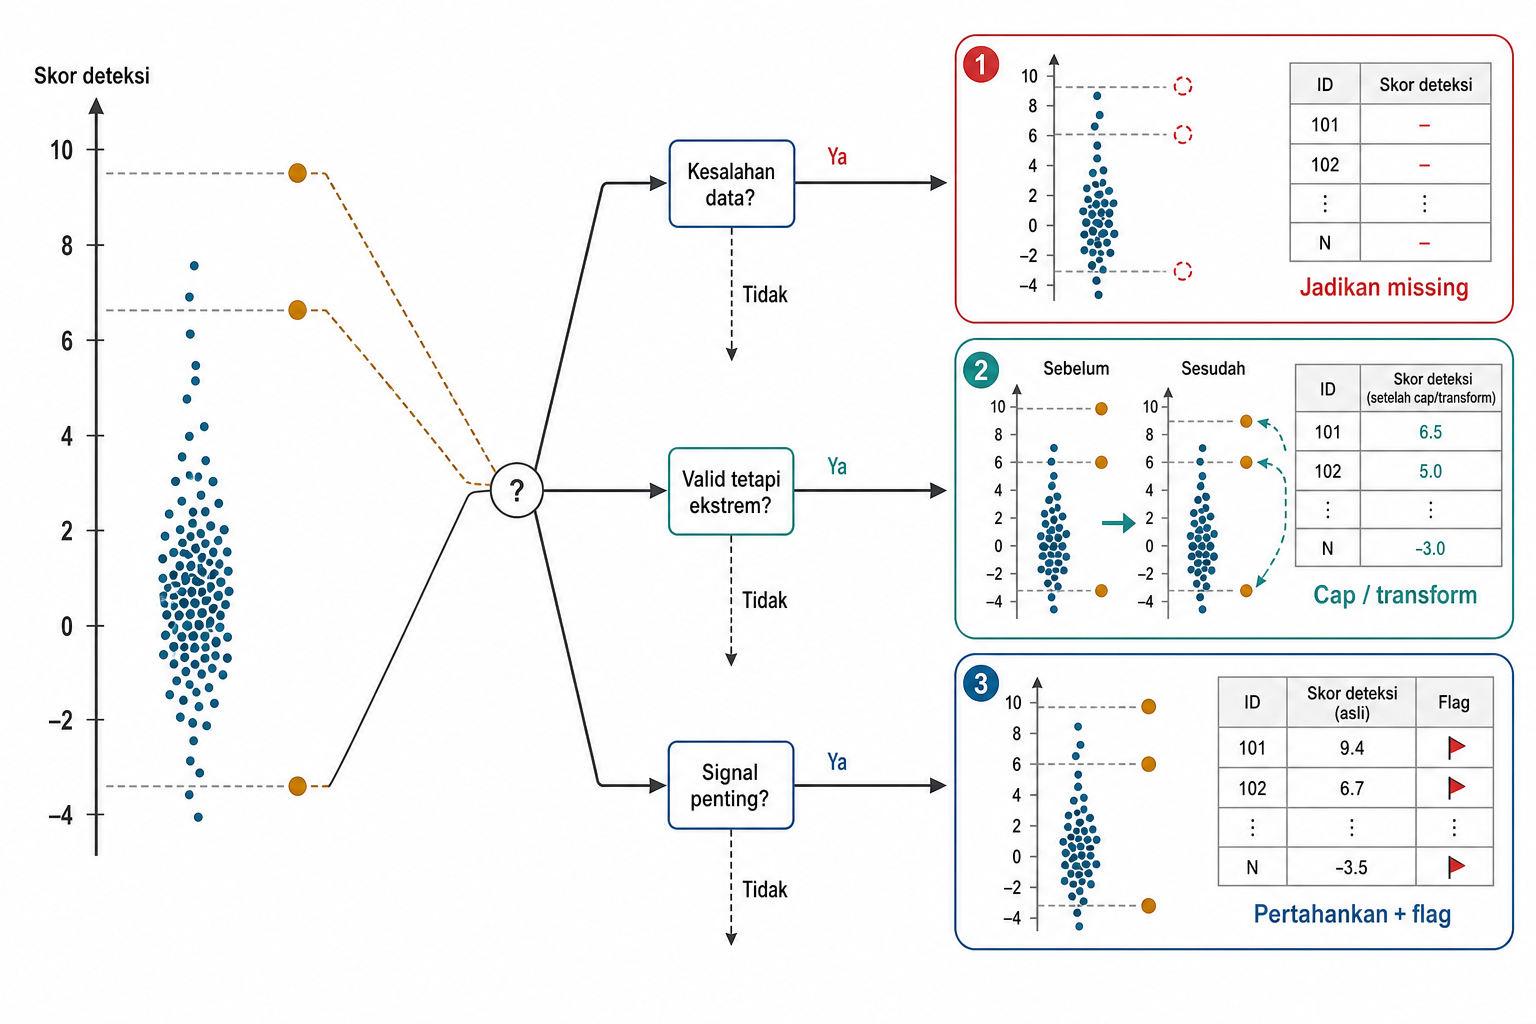
\includegraphics[width=\linewidth,height=0.72\textheight,keepaspectratio]{ch05-fig-5}
\caption{Alur Transformasi Satu Fitur Asli Menjadi Fitur Berimputasi dan Missing Indicator}
\label{fig:ch05-fig-5}
\end{figure}

Pendekatan ini sangat relevan saat menangani mekanisme data \emph{Missing Not At Random} (MNAR), di mana pola kekosongan memiliki korelasi dengan variabel target. Sebagai contoh, pada model penilaian risiko kredit, ketiadaan data ``nomor telepon tempat kerja'' sering kali bukan akibat kegagalan pencatatan sistem. Kekosongan tersebut dapat mengindikasikan riwayat pekerjaan yang tidak stabil, yang secara empiris merupakan sinyal probabilitas gagal bayar yang tinggi.

Keberadaan \emph{missing indicator} mengubah cara model membaca \emph{dataset} yang telah diimputasi. Algoritma akan menggunakan \emph{feature} hasil imputasi untuk mengidentifikasi pola pada populasi umum, sembari di saat yang sama memanfaatkan matriks indikator biner ini untuk menyesuaikan probabilitas prediksi berdasarkan fenomena ketiadaan informasi tersebut. Pada model berbasis pohon (seperti \emph{Random Forest} atau \emph{Gradient Boosting}), tersedianya indikator ini memungkinkan algoritma membuat partisi percabangan logika (\emph{split}) spesifik yang membedakan observasi dengan nilai asli dari observasi dengan nilai tebakan hasil perkiraan.

Secara teknis, komputasi indikator ini umumnya dirangkai dalam satu paket dengan objek imputasi di dalam \emph{pipeline} (seperti mengaktifkan parameter \passthrough{\lstinline!add_indicator=True!} pada \passthrough{\lstinline!SimpleImputer!} di pustaka Scikit-Learn). Pembentukan indikator tunduk pada batasan fiksasi \emph{fit-transform} untuk mencegah \emph{data leakage}. Pertama, \emph{feature} indikator ini dikunci secara fiksasi saat pelatihan; matriks biner hanya diregistrasi untuk kolom-kolom yang secara empiris terdeteksi memiliki nilai kosong di dalam set pelatihan (\emph{training set}). Kedua, terdapat kekakuan saat inferensi; jika sebuah kolom terisi penuh di data pelatihan namun secara mengejutkan muncul dengan nilai kosong pada data baru di lingkungan produksi, \emph{pipeline} tidak akan mengizinkan pembentukan kolom indikator baru secara dadakan, melainkan hanya akan menjalankan fungsi imputasinya saja.

Penggunaan \emph{missing indicator} memiliki konsekuensi komputasi yang menuntut evaluasi struktural terukur. Praktisi wajib menggunakannya secara cermat dengan mengantisipasi dua konsekuensi spasial. Risiko pertama berupa penambahan indikator redundan yang mengekspansi skala dimensi fitur secara berlebih (karena imputasi MCAR meratakan proporsi tanpa menambah acuan korelasi spesifik) tanpa menambahkan tingkat sinyal signifikansi terhadap variabel \emph{dataset}. Risiko sekunder terletak pada pembentukan multikolinearitas struktural fungsional matriks linear. Kondisi \emph{dataset} yang menghapus data indikator dalam kombinasi parameter seragam berbarengan secara independen (\emph{co-missing patterns})--misalnya tanggal masuk kontrak tercatat bersama kolom keluarnya dari rentang operasional--berakibat parameter indikator yang sama pada fungsi korelasinya mengalami garis keselarasan konstan absolut. Kelemahan kalkulasi multikolinearitas mengganggu kestabilan arah konvergensi optimisasi saat dioperasikan memakai metode linear regresi atau algoritma parametrik murni lainnya.

\section{\texorpdfstring{\emph{Outlier}: Deteksi vs.~Penanganan}{Outlier: Deteksi vs.~Penanganan}}\label{outlier-deteksi-vs.-penanganan}

Selain penanganan \emph{missing values}, nilai ekstrem atau \emph{outlier} merupakan tantangan utama dalam merepresentasikan distribusi populasi. \emph{Outlier} kerap diperlakukan sebagai data rusak yang harus segera dihapus. Praktik pembersihan reaktif ini berisiko menghilangkan varians data. Rekayasa \emph{feature} yang sistematis membagi manajemen \emph{outlier} ke dalam dua tahap operasional terpisah: deteksi dan penanganan.

\textbf{Deteksi: Mengobservasi Anomali.}\label{deteksi-mengobservasi-anomali}

Tahap deteksi murni bertujuan menetapkan batas kenormalan suatu \emph{feature}. Algoritma hanya melabeli atau memberikan skor pada nilai yang secara matematis berada di luar distribusi mayoritas, tanpa melakukan modifikasi nilai.

Ekosistem analitik data mengelompokkan pendekatan deteksi \emph{outlier} ke dalam beberapa tingkatan perhitungan algoritma komputasi. Pendekatan pertama didasari pengukuran univariat, yang menganalisis rasio pusat distribusi melalui penerapan batasan ambang matematis interkuartil (IQR). Pada observasi ruang multi-dimensi fungsional, metode pendekatan kedua yaitu analisis multivariat dieksekusi dengan mendayagunakan metode \emph{Isolation Forest} dan perhitungan jarak batas ruang variabel \emph{Local Outlier Factor} (LOF). Evaluasi \emph{Isolation Forest} membedah rentang observasi menjadi jarak dimensi pemisahan titik pencilan dari sampel mayoritas dalam kelompok *dataset*, sementara LOF menentukan skor jarak spasial menggunakan nilai proksimal kepadatan dimensi dari matriks bertingkat tersebut. Untuk kebutuhan komputasi skala rasio tanpa perhitungan metrik absolut manual, tingkat yang ketiga memanfaatkan pendekatan probabilitas observasional. Implementasi \emph{Empirical-CDF-based Outlier Detection} (ECOD) menghasilkan batas deteksi anomali pada ruang kumulatif titik dimensi spasial yang menekan kebutuhan parameter penyetelan fungsional fungsi distribusi secara independen.

Implementasi antarmuka dalam pustaka seperti Scikit-Learn juga membedakan skenario analisis anomali ke dalam dua metode. \emph{Outlier detection} melabeli data pelatihan yang memang sudah terkontaminasi anomali sejak awal (umumnya menggunakan fungsi \passthrough{\lstinline!fit_predict!}). Di sisi lain, \emph{novelty detection} membangun profil normal secara eksklusif dari data bersih, lalu menggunakannya untuk mendeteksi penyimpangan hanya pada observasi baru (misalnya dengan memicu parameter \passthrough{\lstinline!novelty=True!} pada LOF).

Untuk data univariat, rata-rata dan deviasi standar mudah terdistorsi oleh nilai ekstrem itu sendiri. Metode yang lebih tangguh (\emph{robust}) mengganti deviasi standar dengan skor Z yang dimodifikasi (\emph{modified z-score}) yang diturunkan dari Deviasi Absolut Median (MAD):

\[ MAD = \text{median}(|x_i - \text{median}(X)|) \]

\[ M_i = \frac{0.6745 \cdot (x_i - \text{median}(X))}{MAD} \]

Dalam persamaan ini, variabel \(x_i\) merepresentasikan nilai observasi \emph{feature} ke-\(i\), sedangkan \(\text{median}(X)\) merupakan nilai tengah dari seluruh observasi \emph{feature} \(X\). Variabel \(MAD\) mengukur variabilitas dari penyebaran data di sekitar median yang kebal terhadap tarikan \emph{outlier}. Terakhir, \(M_i\) adalah metrik anomali observasi; konstanta \(0.6745\) digunakan untuk menyelaraskan metrik ini agar sepadan dengan estimasi deviasi standar pada distribusi normal. Secara empiris, observasi dengan nilai \(|M_i| > 3.5\) umumnya dilabeli sebagai anomali.

\begin{figure}[htbp]\centering
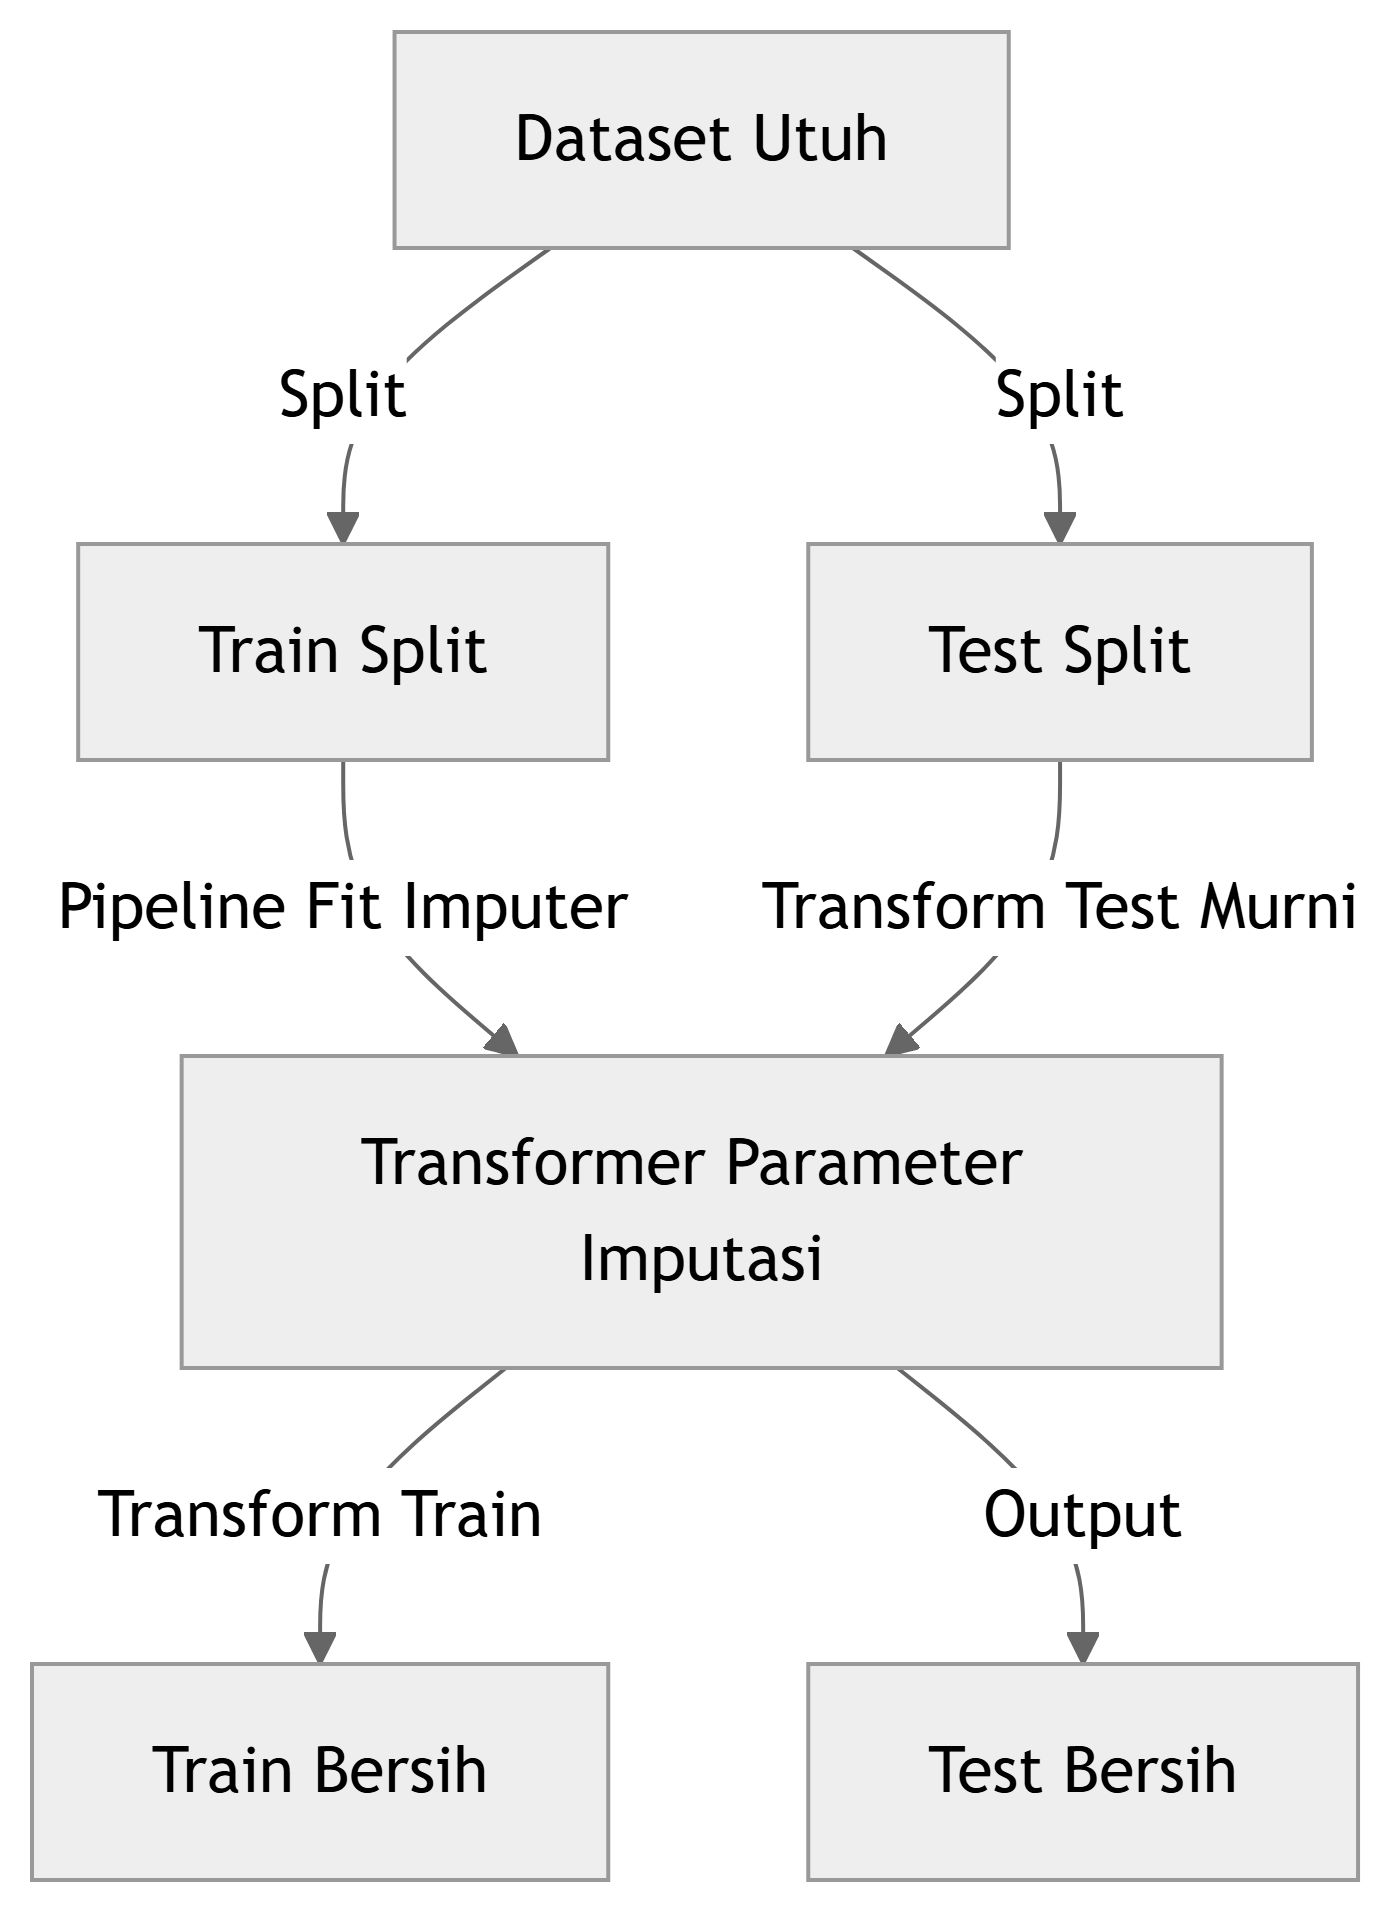
\includegraphics[width=\linewidth,height=0.72\textheight,keepaspectratio]{ch05-fig-6}
\caption{Perbandingan Alur Eksekusi Data Cleaning Statis vs Transformasi Dinamis}
\label{fig:ch05-fig-6}
\end{figure}

\textbf{Penanganan: Konteks Domain.}\label{penanganan-konteks-domain}

Setelah modul matematika mengkalkulasi skor ekstrem, keputusan penyelesaian anomali tidak dipandu murni lewat rentang distribusi komputasi. Konteks riil operasional (*domain knowledge*) dari rentang *dataset* secara spesifik harus mendikte bentuk konversi dan substitusinya. Pada skenario kesalahan sistem pencatatan pengukuran instrumen, seperti observasi umur konsumen negatif atau angka ukuran sensor pada kisaran mustahil secara biologi manusia, baris tersebut secara efektif dikalkulasikan sebagai fitur kolom bernilai \emph{missing value}. Solusinya bisa direalisasikan ke fungsi pemotongan titik maksimum batas operasional (\emph{capping}) dari algoritma. Kasus anomali yang kedua terjadi karena pengamatan tersebut adalah pola sinyal asli matriks data. Perekaman jumlah transfer atau ukuran komputasi batas jutaan transaksi bisa berarti pergerakan nasabah *corporate* khusus (yang secara sah terindikasi *fraud*) pada evaluasi deteksi klasifikasi bank. Kesalahan fatal pada parameter modifikasi imputasi yang tidak seimbang untuk mendepak representasi \emph{outlier} tanpa dasar akan mendistorsi prediksi evaluasi akhir dan parameter optimisasi batas fungsi \emph{machine learning}. Pemisahan titik isolasi fungsional parameter batas pengurungan dari metode intervensi perhitungan nilai menjamin kalkulasi parameter asli dan mengembalikan signifikansi rentang *machine learning* secara utuh.

\section{\texorpdfstring{Transformasi \emph{Robust} untuk \emph{Outlier}}{Transformasi Robust untuk Outlier}}\label{transformasi-robust-untuk-outlier}

\emph{Outlier} yang faktual dan valid menimbulkan dilema. Menghapus observasi membuang informasi dan mengurangi ukuran sampel data. Sebaliknya, membiarkan nilai ekstrem apa adanya dapat mendistorsi pelatihan. Algoritma yang sensitif terhadap magnitudo (seperti regresi linier atau metode berbasis jarak) rentan terhadap efek ini karena fungsi kerugiannya memberikan penalti besar pada titik ekstrem. Akibatnya, garis regresi tertarik kuat ke arah \emph{outlier} hanya untuk meminimalkan kerugian pada titik tersebut, sehingga mengorbankan akurasi mayoritas data. Transformasi \emph{robust} meredam pengaruh nilai ekstrem ini tanpa menghilangkan informasi posisinya.

Terdapat tiga metode utama untuk menangani nilai ekstrem melalui pendekatan transformasi.

Metode pertama adalah pemangkasan (\emph{capping} atau \emph{winsorizing}). Daripada membuang baris data, kita menetapkan ambang batas atas dan batas bawah; setiap nilai yang melampauinya dipangkas dan disamakan dengan batas tersebut. Sebagai contoh, jika batas ditetapkan pada persentil ke-99, observasi pendapatan yang melebihi titik tersebut diubah menjadi sama persis dengan nilai persentil itu. Individu terkait tetap berada di kelompok teratas, tetapi magnitudo absolutnya terkendali. Implementasi yang sejalan dengan praktik \emph{pipeline} yang benar akan mempelajari batas pemangkasan ini murni dari data latih dan menerapkannya kembali secara persis pada saat pemrosesan data uji.

Ambang batas pemangkasan ini umumnya dihitung menggunakan tiga jenis pendekatan matematis. Pendekatan berbasis kuantil memotong distribusi menurut proporsi absolut, misalnya menyisihkan 1\% data terendah dan tertinggi. Pendekatan berbasis Rentang Antarkuartil (IQR) menggunakan rentang antar-persentil sebagai basis turunan pagar anomali Tukey. Sementara itu, pendekatan berbasis Deviasi Absolut Median (MAD) menjadi alternatif \emph{robust} dari standar deviasi konvensional. Standar deviasi biasa akan terdistorsi jika dihadapkan pada \emph{outlier} ekstrem karena nilai ekstrem tersebut otomatis ikut membesarkan hasil kalkulasi rata-rata dan varians; perhitungan berbasis MAD kebal terhadap distorsi tersebut karena ia bersandar kuat pada pengukuran median.

Persamaan \emph{modified z-score} menggunakan rumusan:

\[ M_i = \frac{0.6745 \cdot (x_i - \tilde{x})}{\text{MAD}} \]

Dalam formulasi tersebut, variabel \(M_i\) mewakili skor modifikasi untuk observasi ke-\(i\), \(x_i\) adalah nilai titik data, \(\tilde{x}\) adalah median dari distribusi \emph{feature}, dan \(\text{MAD}\) merupakan deviasi absolut median itu sendiri (yakni median dari selisih absolut setiap observasi terhadap \(\tilde{x}\)). Faktor \(0.6745\) digunakan semata-mata untuk menyejajarkan skor dengan rentang distribusi normal baku. Titik data yang melewati rentang absolut \(|M_i| > 3.5\) biasanya dipangkas atau ditandai sebagai \emph{outlier}.

\begin{figure}[htbp]\centering
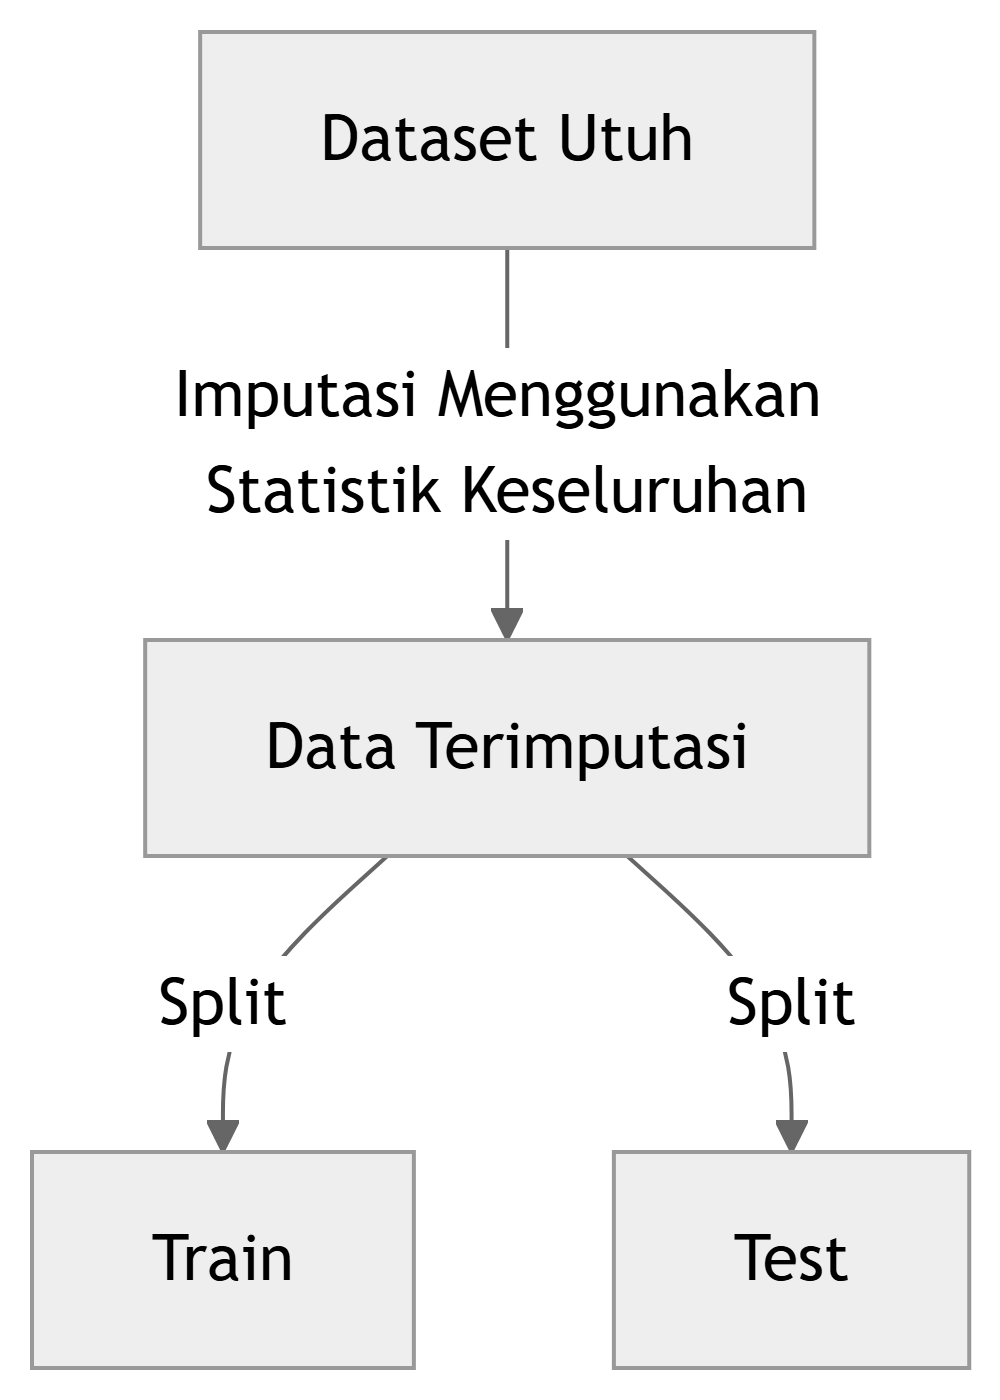
\includegraphics[width=\linewidth,height=0.72\textheight,keepaspectratio]{ch05-fig-7}
\caption{Arsitektur Pipeline Pemrosesan Data: Aliran X\_train dan X\_test}
\label{fig:ch05-fig-7}
\end{figure}

Selain pemangkasan, penyesuaian distribusi \emph{feature} melalui penskalaan juga lazim digunakan. Metode kedua adalah penskalaan \emph{robust} (\emph{robust scaling}). Penskalaan standar berbasis \emph{z-score} menjadi sangat rentan karena rata-rata dan standar deviasinya terseret oleh \emph{outlier}. Penskalaan \emph{robust} memusatkan data dengan median dan menskalakannya menggunakan IQR. Pengukuran ini murni memakai titik data di pusat distribusi (persentil ke-25 sampai ke-75), yang membuat skala \emph{feature} tetap stabil meskipun terdapat deretan nilai ekstrem di ujung rentang distribusi.

Metode ketiga adalah pemampatan distribusi (\emph{log / power transform}). Memampatkan skala terbukti efektif memfasilitasi data yang didominasi nilai kecil namun memiliki ekor panjang ke sisi kanan. Transformasi logaritmik atau penerapan \emph{power transform} menekan nilai-nilai dominan ekstrem agar rentang magnitudonya bergeser mendekati sisa distribusi mayoritas. Operasi ini mengecilkan jarak absolut antar-observasi tanpa mendisrupsi urutan ordinal; nilai maksimal tetap di puncak, sehingga model tidak terdistorsi akibat besaran asimetris saat pelatihan.

\section{\texorpdfstring{Batas Antara \emph{Data Cleaning} dan Rekayasa \emph{Feature}}{Batas Antara Data Cleaning dan Rekayasa Feature}}\label{batas-antara-data-cleaning-dan-rekayasa-feature}

Dalam alur kerja ilmu data, batasan antara \emph{data cleaning} dan rekayasa \emph{feature} kerap beririsan karena keduanya bertugas mengubah wujud data mentah sebelum dieksekusi oleh model \emph{machine learning}. Pemahaman tentang batas operasional kedua proses ini berguna untuk merancang \emph{pipeline} yang kebal terhadap \emph{data leakage}, sekaligus mendefinisikan ruang lingkup teknis yang dibahas dalam buku ini.

\emph{Data cleaning} berfokus pada koreksi fakta untuk memastikan sebuah \emph{dataset} merepresentasikan keadaan dunia nyata secara akurat. Validitas dari pembersihan data bersifat mutlak dan tidak akan berubah meskipun kita mengganti algoritma pemodelan. Pertama, perbaikan ini terfokus pada fakta yang salah, format yang tidak konsisten, atau duplikasi entitas. Kedua, titik eksekusinya bersifat statis dan global; ia dieksekusi satu kali pada keseluruhan data sebelum proses pemodelan atau pembagian data dimulai. Contoh tindakannya meliputi mengurai teks \emph{string} ``1,200.50'' agar terbaca secara benar sebagai nilai numerik, menghapus observasi usia 150 tahun yang mustahil secara biologis, atau melakukan deduplikasi terhadap baris data yang tercatat berulang akibat kesalahan sistem pencatatan.

Di sisi lain, rekayasa \emph{feature} beroperasi di ranah representasi. Fokus utamanya bukan lagi menguji kebenaran fakta dasar, melainkan memanipulasi bentuk data agar algoritma dapat mengekstrak sinyal darinya dengan efisien. Pertama, manipulasi ini bertujuan mengubah distribusi, skala, atau format representasi sebagai keputusan desain yang disesuaikan secara khusus dengan kebutuhan algoritma tertentu. Kedua, titik eksekusinya bersifat dinamis dan harus diikat kuat di dalam \emph{pipeline} pembelajaran untuk menjaga batasan isolasi data latih. Contoh tindakannya mencakup mengaplikasikan \emph{robust scaler} pada sebuah \emph{feature} agar metrik jarak SVM dapat konvergen, mencetak \emph{missing indicator} baru untuk menampung sinyal informasi, atau melakukan imputasi nilai yang hilang berdasarkan pola distribusi observasi latih.

Kriteria pembatas operasional paling tegas antara kedua proses ini bersandar pada literatur kebocoran data (IBM, 2024), yakni dengan mengajukan satu pengujian: apakah transformasi tersebut bergantung pada pembagian \emph{train/test split}?

Secara matematis, perbedaan sifat eksekusi ini dapat dirumuskan melalui definisi fungsi pemrosesan:

\[
X_{bersih} = C(X_{mentah}) \quad \text{vs} \quad X_{\text{feature}} = T_{\theta}(X_{bersih})
\]

Fungsi pembersihan \(C\) diterapkan secara seragam pada seluruh observasi \(X_{mentah}\) tanpa mengamati interaksi antar-baris. Sebaliknya, transformasi \emph{feature} \(T\) dikendalikan oleh matriks parameter \(\theta\) (misalnya batas parameter kuartil pada \emph{scaler} atau nilai rata-rata pada imputer) yang secara eksklusif dipelajari hanya dari subset data latih. Menghitung \(\theta\) menggunakan data pengujian adalah asal mula terjadinya \emph{data leakage}.

Batas operasional ini juga membatasi cakupan materi yang dieksplorasi di dalam bab-bab berikutnya. Buku ini tidak membahas tutorial manipulasi teks mentah, penggunaan fungsi \emph{regex} untuk menyortir format kotor, atau instruksi teknik deduplikasi basis data. Titik berat kita dikhususkan sepenuhnya pada desain dan penerapan operasional \(T_{\theta}\), yakni rekayasa representasi yang berinteraksi langsung dengan mekanisme pembelajaran mesin.

\section{\texorpdfstring{Studi Kasus: \emph{Pipeline} Imputasi dan Penanganan \emph{Robust} yang \emph{Reproducible}}{Studi Kasus: Pipeline Imputasi dan Penanganan Robust yang Reproducible}}\label{studi-kasus-pipeline-imputasi-dan-penanganan-robust-yang-reproducible}

Penerapan taktik penanganan \emph{missing values} dan \emph{outlier} secara terpisah pada tahap prapemrosesan rentan memicu \emph{data leakage}. Jika kalkulasi batas \emph{outlier} atau rata-rata imputasi dilakukan sebelum membagi set pelatihan dan pengujian, informasi dari set pengujian akan ikut merembes dan memengaruhi model. Untuk mencegah kontaminasi ini, seluruh komponen transformasi harus disatukan ke dalam arsitektur \emph{pipeline}.

Sebagai contoh, tinjau sebuah \emph{dataset} medis untuk prediksi risiko penyakit yang memiliki dua anomali struktural:

\begin{enumerate}
\def\labelenumi{\arabic{enumi}.}
\tightlist
\item
  \textbf{Ketiadaan data yang tidak acak:} \emph{Feature} ``jumlah tes darah'' mengandung \emph{missing values} bertipe \emph{Missing Not At Random} (MNAR). Pasien berisiko tinggi lebih sering menjalani observasi laboratorium. Kekosongan data di kolom ini merepresentasikan ketiadaan tes karena pasien relatif sehat.
\item
  \textbf{Ekor distribusi yang panjang:} \emph{Feature} ``kadar protein'' memiliki nilai ekstrem yang valid secara biologis, bukan akibat kesalahan sensor. Jika tidak dibatasi, magnitudo ekstrem ini akan mengganggu konvergensi dan stabilitas skala model linier.
\end{enumerate}

Berdasarkan diagnosis di atas, kita merancang spesifikasi \emph{pipeline} berurutan:

\begin{enumerate}
\def\labelenumi{\arabic{enumi}.}
\tightlist
\item
  \textbf{Ekstraksi indikator:} Menambahkan \passthrough{\lstinline!MissingIndicator!} (atau mengaktifkan argumen \passthrough{\lstinline!add_indicator=True!} pada objek imputer) untuk menyalin lokasi sel yang kosong menjadi sebuah \emph{feature} biner baru.
\item
  \textbf{Imputasi berbasis model:} Menjalankan algoritma \passthrough{\lstinline!IterativeImputer!} atau \passthrough{\lstinline!KNNImputer!} untuk menaksir nilai numerik pada sel yang kosong dengan memetakan korelasi antar-atribut medis.
\item
  \textbf{Pembatasan ekstrem (\emph{capping}):} Menerapkan objek \passthrough{\lstinline!Winsorizer!} untuk memangkas magnitudo nilai di atas batas persentil ke-95.
\item
  \textbf{Penyesuaian skala (\emph{scaling}):} Melakukan standardisasi dengan \passthrough{\lstinline!RobustScaler!} menggunakan perhitungan median dan \emph{Interquartile Range} (IQR), sehingga skala \emph{feature} akhir tetap stabil terhadap sisa residu \emph{outlier}.
\end{enumerate}

Secara matematis, \emph{pipeline} mengeksekusi komposisi fungsi transformasi secara berantai pada data observasi (\(X_{\text{in}}\)). Parameter transformasi di setiap tahap akan dikunci dengan mengandalkan statistik yang dipelajari mutlak dari data latih melalui persamaan \(X_{\text{out}} = T_n(T_{n-1}( \dots T_1(X_{\text{in}} \mid \theta_1) \dots \mid \theta_{n-1}) \mid \theta_n)\). Pada perumusan tersebut, \(T_i\) adalah representasi matematis dari fungsi transformasi pada tahap ke-\(i\) (seperti fungsi pemotongan distribusi atau fungsi pergeseran skala), dan \(\theta_i\) mewakili parameter statistik spesifik (seperti batas kuantil, median, atau bobot imputasi) yang dikalkulasi secara eksklusif saat algoritma memproses \emph{split} pelatihan. Pemanggilan fungsi \passthrough{\lstinline!fit()!} pada blok \emph{pipeline} akan merekam pola indikator variabel, distribusi relasional, dan batas persentil tanpa melihat satu pun observasi dari set pengujian. Saat dieksekusi di dalam skema \emph{cross-validation}, struktur ini memaksa prosedur imputasi dan estimasi statistik beroperasi secara terisolasi murni di dalam setiap porsi lipatan (\emph{fold}).

Sebagai catatan evaluasi teknis, literatur menunjukkan satu pengecualian: metode imputasi univariat statis tanpa pengawasan (seperti imputasi nilai rata-rata biasa) yang dieksekusi sebelum pemisahan lipatan \emph{cross-validation} memang terkadang memunculkan bias yang dapat diabaikan sembari mempercepat komputasi. Namun, untuk metode imputasi iteratif dan tersupervisi, keseluruhan kalkulasinya wajib diletakkan secara ketat di dalam \emph{pipeline} guna menghindari ilusi akurasi evaluasi yang fiktif.

\begin{lstlisting}[language=Python]
import numpy as np
import pandas as pd
from sklearn.base import BaseEstimator, TransformerMixin
from sklearn.experimental import enable_iterative_imputer  # Wajib diimpor sebelum IterativeImputer
from sklearn.impute import IterativeImputer
from sklearn.preprocessing import RobustScaler
from sklearn.pipeline import Pipeline

class Winsorizer(BaseEstimator, TransformerMixin):
    """
    Transformer kustom untuk memotong (cap/clip) nilai outlier ekstrem 
    berdasarkan nilai persentil batas bawah dan batas atas.
    """
    def __init__(self, lower_quantile=0.05, upper_quantile=0.95):
        self.lower_quantile = lower_quantile
        self.upper_quantile = upper_quantile
        self.lower_bounds_ = None
        self.upper_bounds_ = None
        
    def fit(self, X, y=None):
        X_df = pd.DataFrame(X)
        self.lower_bounds_ = X_df.quantile(self.lower_quantile).values
        self.upper_bounds_ = X_df.quantile(self.upper_quantile).values
        return self
        
    def transform(self, X):
        X_df = pd.DataFrame(X).copy()
        for col_idx in range(X_df.shape[1]):
            X_df.iloc[:, col_idx] = np.clip(
                X_df.iloc[:, col_idx], 
                self.lower_bounds_[col_idx], 
                self.upper_bounds_[col_idx]
            )
        return X_df.values

# Membangun arsitektur pipeline pemrosesan data medis terintegrasi
medical_pipeline = Pipeline([
    ('imputer', IterativeImputer(max_iter=10, random_state=42, add_indicator=True)),
    ('outlier_clipper', Winsorizer(lower_quantile=0.01, upper_quantile=0.95)),
    ('scaler', RobustScaler())
])

# Simulasi data medis pasien (misalnya: Tekanan Darah, Kadar Gula Darah, Kadar Protein)
np.random.seed(42)
X_raw = np.random.normal(loc=100, scale=20, size=(100, 3))
X_raw[0, 0] = 400.0  # Sisipkan outlier ekstrem atas
X_raw[1, 1] = 2.0    # Sisipkan outlier ekstrem bawah
X_raw[5:15, 0] = np.nan  # Sisipkan missing values (NaN)
X_raw[12:20, 2] = np.nan

# Melatih pipeline sekaligus mentransformasikan data latih secara aman
X_processed = medical_pipeline.fit_transform(X_raw)

print(f"Dimensi data asli: {X_raw.shape}")
print(f"Dimensi data terproses (termasuk kolom indikator missing): {X_processed.shape}")
print(f"Nilai maksimum setelah pemrosesan: {np.max(X_processed):.4f}")
\end{lstlisting}

\section{Sintesis Keputusan dan Prinsip Akhir}\label{sintesis-keputusan-dan-prinsip-akhir}

Penanganan nilai kosong dan pencilan adalah perpaduan antara kehati-hatian statistik, pemahaman konteks domain, dan kedisiplinan integrasi \emph{pipeline}.

\textbf{Strategi Pengisian Nilai Kosong.} Diagnosis pola kekosongan terlebih dahulu sebelum memilih metode. Pada skenario MCAR, imputasi univariat sederhana (rata-rata/median) cukup memadai dan efisien. Jika korelasi antar-variabel kuat (MAR), terapkan imputasi multivariat (seperti KNN atau MICE) agar struktur distribusi asli tetap terjaga. Pada kondisi MNAR, ketiadaan data sering kali menyimpan informasi penting; pertahankan sinyal tersebut dengan mengonstruksi \emph{feature} biner pendukung berupa \emph{missing indicator}.

\textbf{Manajemen Pencilan.} Deteksi pencilan menggunakan parameter yang kebal terhadap kontaminasi ekstrem (seperti median dan MAD untuk data univariat, atau \emph{Isolation Forest} untuk data berdimensi tinggi). Keputusan intervensi (apakah dipotong lewat \emph{capping/winsorization}, ditransformasi lewat metode \emph{robust}, atau diperlakukan sebagai \emph{missing values}) wajib disesuaikan dengan konteks domain untuk mencegah hilangnya sinyal anomali yang bernilai tinggi (seperti pada deteksi transaksi penipuan).

\textbf{Integrasi Bersih dalam Pipeline.} Seluruh kalkulasi statistik (seperti rata-rata imputasi, median, dan batas kuantil pemotongan) harus diisolasi di dalam objek \emph{pipeline}. Parameter ini dipelajari (\emph{fit}) murni dari himpunan data latih dan diterapkan kembali saat \emph{transform} pada data uji atau data baru di lingkungan produksi. Batasan tegas ini menjamin reproduksibilitas komputasi sekaligus melenyapkan risiko kebocoran data.

Demonstrasi interaktif dan latihan penanganan data renggang secara terstruktur ini dapat diuji secara langsung menggunakan skrip dan data pendamping pada repositori buku ini.

% ==========================================================================
% ch06.tex — dihasilkan otomatis dari website/chapters/ch06.qmd
% Boleh disunting manual. 'sync' hanya menimpa bila .qmd berubah DAN .tex
% belum disunting; kalau keduanya berubah, dilewati (pakai --force).
% qmd-sha1: 46cc42ad3cb8
% tex-sha1: f3e6108d4b0e
% ==========================================================================
% >>>>> ISI OTOMATIS (jangan hapus baris ini) >>>>>
\chapter{Pembentukan Fitur Turunan}\label{pembentukan-fitur-turunan}

\section{Pembentukan Fitur Turunan: Rasio, Selisih, dan Interaksi}\label{pembentukan-fitur-turunan-rasio-selisih-dan-interaksi}

Model \emph{machine learning} sering kali membutuhkan representasi data yang secara eksplisit menghubungkan beberapa variabel. Meskipun arsitektur kompleks mampu memetakan interaksi antar-variabel secara mandiri, proses tersebut menuntut komputasi yang tinggi dan volume data yang besar. Dengan menyediakan representasi yang dirancang manusia ini, model menerima sinyal prediktif secara langsung sehingga konvergensi berjalan lebih cepat.

Fitur turunan diciptakan melalui operasi matematika pada atribut mentah yang sudah ada. Tiga operasi aritmatika dasar yang paling sering diimplementasikan meliputi:

\begin{enumerate}
\def\labelenumi{\arabic{enumi}.}
\tightlist
\item
  \textbf{Selisih (Pengurangan):} Mengukur defisit, sisa, atau perubahan absolut. Algoritma dasar tidak memodelkan selisih dua fitur secara otomatis. Sebagai contoh, memberikan angka pengeluaran bulanan dan pendapatan bulanan secara terpisah kurang informatif dibandingkan membangun fitur tunggal ``pendapatan bersih''. Fitur ini secara langsung mendeskripsikan kapasitas finansial riil sebuah entitas.
\item
  \textbf{Rasio (Pembagian):} Menangkap proporsi relatif dan menormalkan skala metrik. Dalam analisis kelayakan kredit, nilai utang absolut sulit diinterpretasikan tanpa konteks yang menyertainya. Membagi nilai utang terhadap total aset menghasilkan rasio proporsional yang memetakan perusahaan rintisan kecil dan korporasi berskala global pada rentang metrik risiko yang terstandardisasi.
\end{enumerate}

\begin{figure}[htbp]\centering
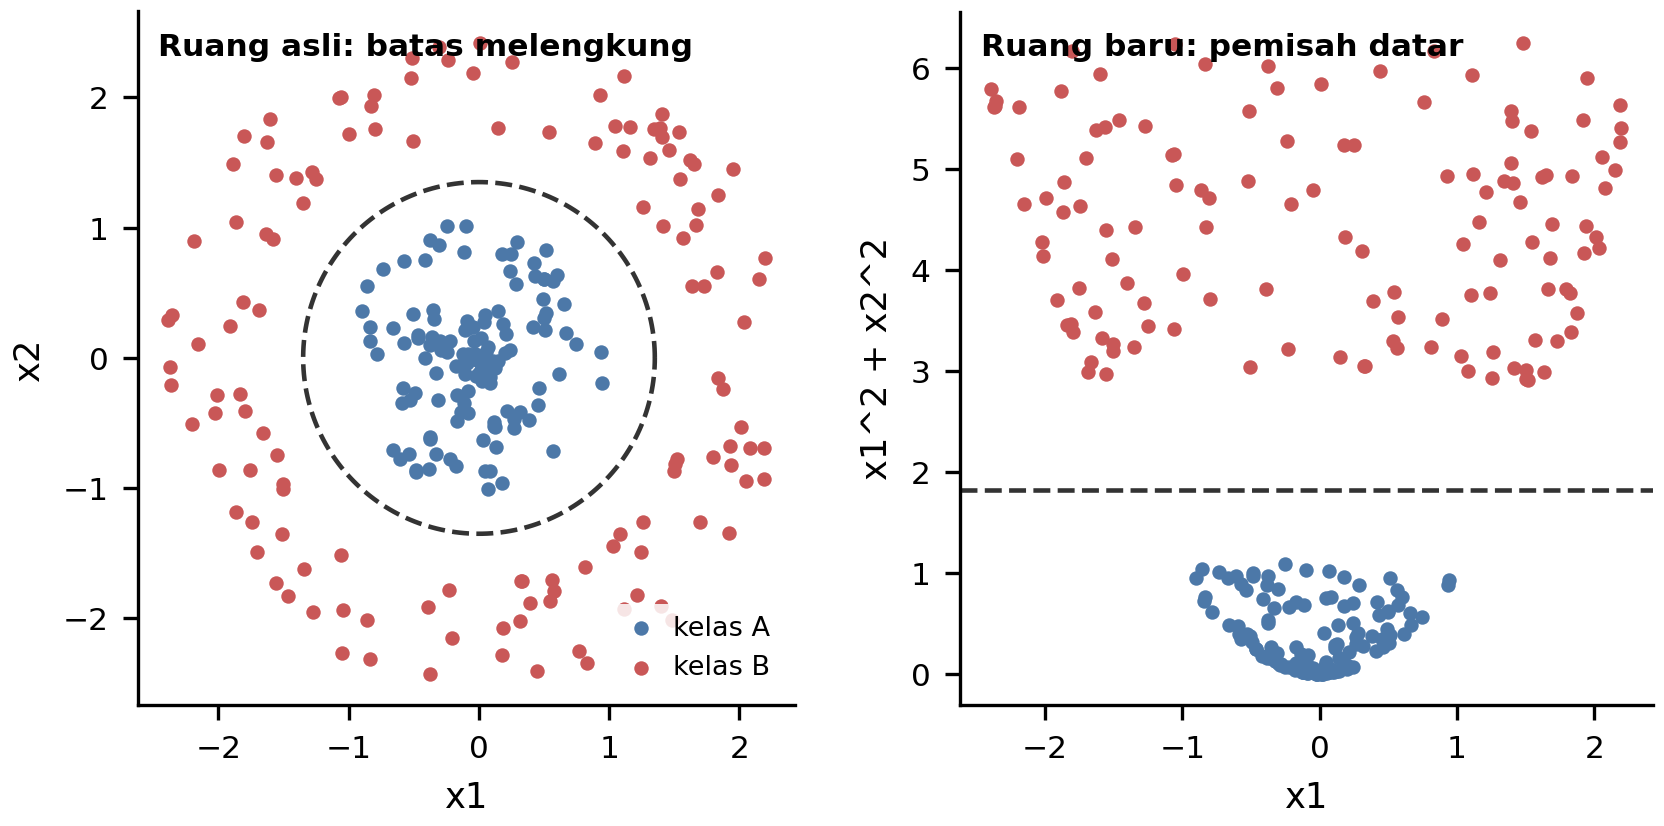
\includegraphics[width=\linewidth,height=0.72\textheight,keepaspectratio]{ch06-fig-1}
\caption{Representasi Rasio Finansial untuk Menormalkan Metrik Berskala Absolut Berbeda}
\label{fig:ch06-fig-1}
\end{figure}

\begin{enumerate}
\def\labelenumi{\arabic{enumi}.}
\setcounter{enumi}{2}
\tightlist
\item
  \textbf{Interaksi (Perkalian):} Menangkap efek gabungan dua atribut yang memiliki dampak di luar penjumlahan linier biasa. Efek perkalian ini direpresentasikan secara matematis sebagai:
\end{enumerate}

\[ x_{interaksi} = x_i \times x_j \]

Di mana \(x_{interaksi}\) adalah turunan fitur baru, sedangkan \(x_i\) dan \(x_j\) merupakan fitur asal. Pada kasus prediksi harga properti, fitur ``usia bangunan'' (\(x_i\)) dapat dikalikan dengan penanda biner ``butuh perbaikan struktural'' (\(x_j\)). Hasilnya membentuk penalti harga eksponensial bagi rumah tua yang sekaligus memiliki struktur rusak - sebuah pola yang menjadi dasar bagi pembentukan turunan polinomial pada derajat yang lebih tinggi.

Pada tingkat produksi, transformasi ini jarang ditulis secara manual secara per-kolom. Pustaka transformasi modern menyertakan modul khusus - seperti \passthrough{\lstinline!RelativeFeatures!} atau \passthrough{\lstinline!MathFeatures!} pada Feature-engine - untuk mengeksekusi operasi selisih, rasio, dan interaksi secara terintegrasi di dalam sebuah \emph{pipeline}. Pendekatan yang lebih mutakhir (seperti CAAFE) bahkan menggunakan \emph{Large Language Models} guna mengusulkan rasio dan interaksi berdasarkan pemahaman semantik nama kolom. Kendati otomatisasi ini mempercepat eksplorasi fitur, pembangkitan turunan yang agresif rentan menimbulkan masalah redundansi, sehingga metode seleksi ketat wajib disertakan setelahnya.

\section{Fitur Polinomial: Ekspresivitas versus Ledakan Fitur}\label{fitur-polinomial-ekspresivitas-versus-ledakan-fitur}

Fitur interaksi yang telah dibahas sebelumnya adalah bentuk sederhana dari ekspansi polinomial. Fitur polinomial memperluas konsep ini dengan memangkatkan fitur asli hingga derajat tertentu, sekaligus mengalikan kombinasi antarfitur tersebut.

Sebagai contoh, jika sebuah dataset memiliki dua fitur dasar, \(x_1\) dan \(x_2\), ekspansi polinomial derajat dua tidak hanya menghasilkan fitur interaksi \(x_1 x_2\), tetapi juga fitur kuadrat dari masing-masing variabel:

\[ \phi(x_1, x_2) = [1, x_1, x_2, x_1^2, x_1 x_2, x_2^2] \]

Di mana:

\begin{itemize}
\tightlist
\item
  \(\phi\) merepresentasikan fungsi pemetaan ke ruang fitur baru.
\item
  \(1\) adalah suku bias (konstanta).
\item
  \(x_1\) dan \(x_2\) adalah fitur asli (derajat satu).
\item
  \(x_1^2\) dan \(x_2^2\) adalah fitur kuadrat independen (derajat dua murni).
\item
  \(x_1 x_2\) adalah fitur interaksi.
\end{itemize}

Alasan utama melakukan ekspansi polinomial adalah untuk memberikan kemampuan pada model linier agar dapat mengenali pola non-linier. Banyak algoritma \emph{machine learning} standar berasumsi bahwa batasan keputusan berbentuk garis lurus atau bidang datar. Asumsi ini sering kali gagal menangkap realitas data yang membentuk kurva.

Dengan memproyeksikan data ke ruang dimensi yang lebih tinggi melalui fitur berpangkat, model linier sederhana menjadi mampu merumuskan batasan keputusan yang melengkung mengikuti kontur data, tanpa perlu mengubah arsitektur dasarnya.

\begin{figure}[htbp]\centering
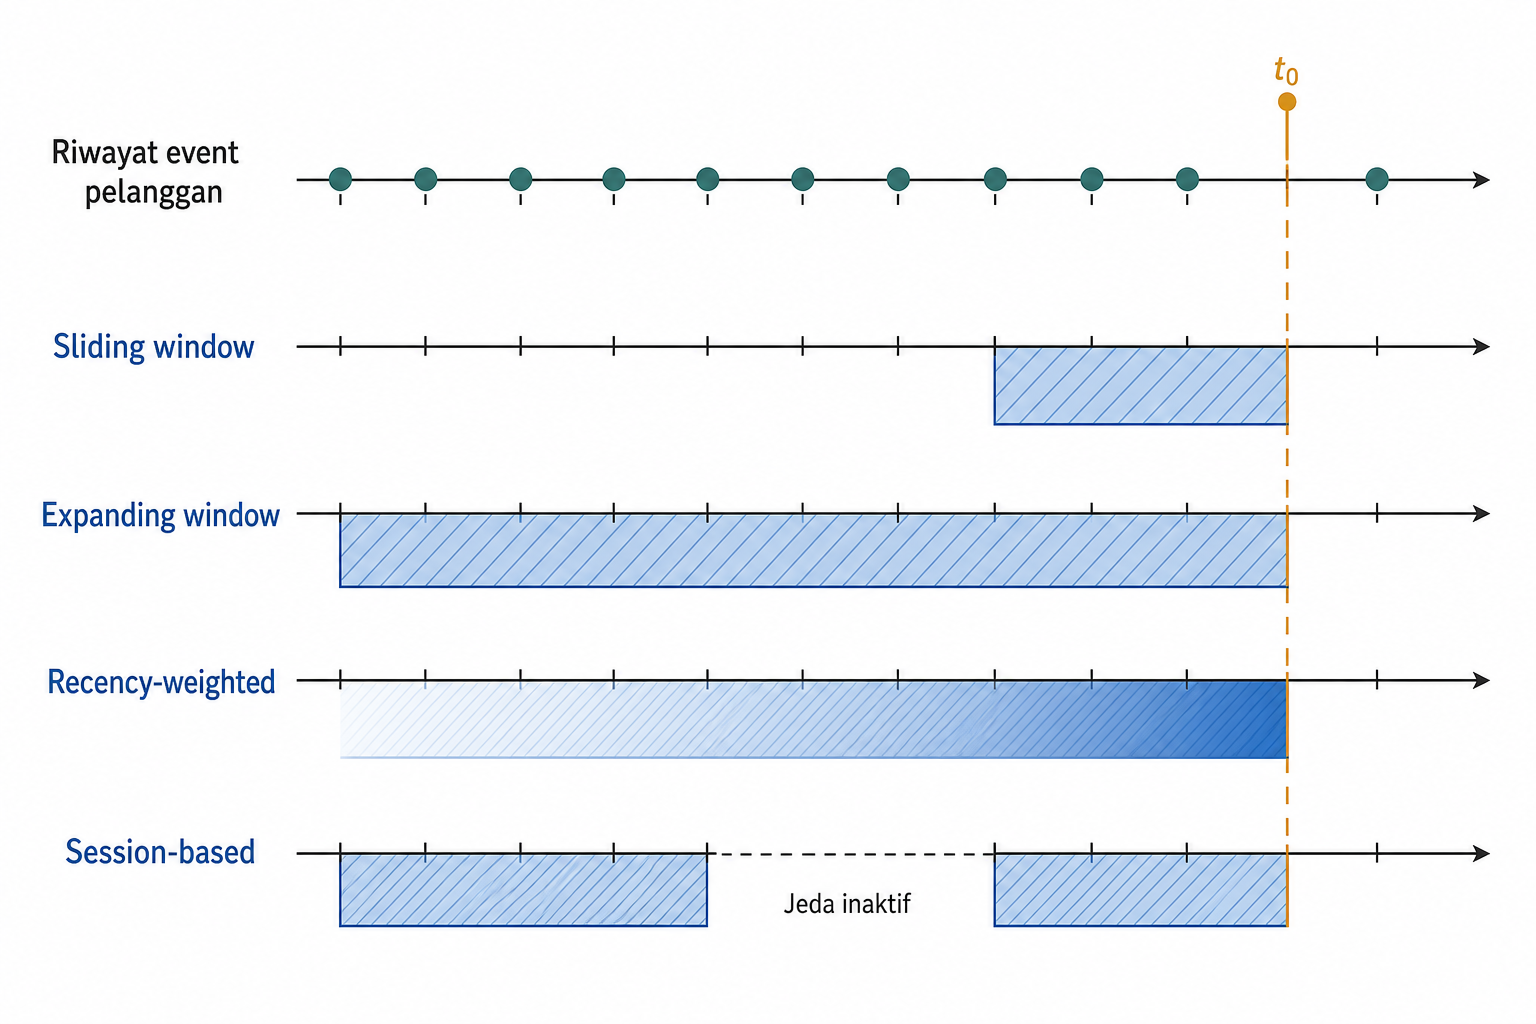
\includegraphics[width=\linewidth,height=0.72\textheight,keepaspectratio]{ch06-fig-2}
\caption{Proyeksi Geometri Ruang Fitur Polinomial dari Dimensi 2D ke 3D}
\label{fig:ch06-fig-2}
\end{figure}

\begin{lstlisting}[language=Python]
import pandas as pd
from sklearn.preprocessing import PolynomialFeatures

# 1. Menyiapkan data observasi sederhana (2 fitur numerik asal)
data = {
    'Kecepatan_Kendaraan': [40, 60, 80],
    'Konsumsi_Bahan_Bakar': [8, 12, 18]
}
df = pd.DataFrame(data)

# 2. Inisiasi objek PolynomialFeatures dengan derajat 2
# include_bias=False membuang kolom bias (bernilai 1) untuk fokus pada interaksi murni
poly = PolynomialFeatures(degree=2, include_bias=False)

# 3. Menjalankan proses fit_transform pada data observasi
X_poly = poly.fit_transform(df)

# 4. Mengekstraksi nama-nama fitur baru hasil ekspansi polinomial
feature_names = poly.get_feature_names_out(df.columns)

# 5. Membungkus hasil transformasi ke dalam DataFrame agar rapi
df_poly = pd.DataFrame(X_poly, columns=feature_names)

print("--- Data Asli ---")
print(df)
print("\n--- Hasil Ekspansi Polinomial (Derajat 2) ---")
print(df_poly.round(2))
\end{lstlisting}

Meskipun meningkatkan ekspresivitas, metode ini membawa \emph{trade-off} utama: risiko ledakan fitur (\emph{feature explosion}). Jumlah fitur turunan tumbuh secara kombinatorial seiring bertambahnya fitur asli dan naiknya derajat polinomial.

Pertumbuhan eksponensial ini memicu tiga masalah operasional dalam \emph{pipeline} rekayasa fitur:

\begin{enumerate}
\def\labelenumi{\arabic{enumi}.}
\tightlist
\item
  \textbf{Konsumsi Memori:} Dataset dengan 100 fitur awal yang diekspansi ke derajat dua akan membengkak menjadi lebih dari 5.000 fitur baru. Kenaikan ke derajat tiga menghasilkan lebih dari 170.000 fitur turunan, yang sering kali langsung membebani kapasitas RAM.
\item
  \textbf{Beban Komputasi:} Waktu pelatihan model melambat secara drastis karena algoritma harus memperbarui bobot untuk ratusan ribu variabel ekstra tersebut.
\item
  \textbf{Risiko Overfitting:} Ketika model disajikan dengan ratusan ribu variasi interaksi buatan, ia cenderung menghafal \emph{noise} pada data latih. Akurasi saat pelatihan mungkin terlihat sangat tinggi, tetapi performa model umumnya langsung turun drastis saat menghadapi data baru di lingkungan produksi.
\end{enumerate}

Untuk mencegah masalah tersebut, ekspansi polinomial sangat jarang diterapkan pada keseluruhan fitur secara serentak. Praktik yang disarankan meliputi:

\begin{enumerate}
\def\labelenumi{\arabic{enumi}.}
\tightlist
\item
  Memilih hanya beberapa fitur spesifik yang terindikasi kuat memiliki hubungan non-linier dengan target.
\item
  Membatasi batas ekspansi pada derajat rendah (umumnya maksimal derajat tiga).
\item
  Melakukan pemangkasan fitur pasca-generasi menggunakan metode seleksi atau regularisasi L1 (\emph{Lasso}) untuk mengeliminasi suku turunan yang tidak relevan.
\end{enumerate}

Pendekatan selektif ini menjaga keseimbangan antara peningkatan akurasi dari pola kompleks dan stabilitas model.

\section{Agregasi dan Fitur Berbasis Kelompok}\label{agregasi-dan-fitur-berbasis-kelompok}

Sebagian besar data mentah hanya merekam informasi pada tingkat observasi tunggal. Model yang hanya melihat satu baris data akan kehilangan konteks situasional. Pola prediktif sering kali baru muncul ketika sebuah observasi diletakkan berdampingan dengan observasi lain di kelompok yang sama. Untuk menghadirkan konteks ini, praktisi menggunakan teknik agregasi, yaitu menghitung metrik statistik (seperti \emph{mean}, \emph{median}, varians) dari partisi kategori tertentu (misalnya ID pengguna atau wilayah geografi), lalu menyematkan nilai tersebut kembali ke setiap anggota kelompok.

Dalam praktiknya, proses agregasi tidak lagi sekadar menghitung rata-rata atau jumlah absolut. Terdapat beberapa pola agregasi mutakhir yang memanfaatkan struktur kelompok, terutama ketika data memiliki dimensi pengurutan atau waktu (\emph{temporal}):

\begin{enumerate}
\def\labelenumi{\arabic{enumi}.}
\tightlist
\item
  \textbf{\emph{Sliding Window}:} Agregasi berbasis jendela mundur berukuran tetap (misalnya, total transaksi dalam ``7 hari terakhir'').
\item
  \textbf{\emph{Expanding Window}:} Agregasi kumulatif dari titik observasi pertama hingga baris saat ini. Pustaka seperti \emph{Feature-engine} menyediakan transformer \passthrough{\lstinline!ExpandingWindowFeatures!} untuk mengeksekusi ini di dalam \emph{pipeline} produksi secara aman.
\item
  \textbf{Pembobotan Kebaruan (\emph{Recency-Weighted Aggregation}):} Tidak semua data historis memiliki bobot relevansi yang setara. Pada agregasi ini, observasi yang lebih baru diberi bobot lebih besar menggunakan fungsi peluruhan eksponensial (\emph{exponential decay}), di mana \(\lambda\) mengontrol tingkat peluruhan berdasarkan jarak waktu (\emph{age}):
  \[ w_i = e^{-\lambda \cdot \text{age}_i} \]
  Rata-rata tertimbang (\emph{weighted mean}) kemudian dihitung dari observasi kelompok tersebut, memungkinkan model bereaksi lebih cepat terhadap perubahan perilaku terbaru.
\item
  \textbf{Reset Berbasis Sesi (\emph{Session-Based Reset}):} Agregasi kumulatif diatur ulang menjadi nol saat terdeteksi periode inaktivitas yang melampaui batas ambang tertentu, memastikan akumulasi metrik hanya mencerminkan sesi aktivitas kontinu.
\end{enumerate}

Ekstraksi fitur agregat dapat dilakukan secara masif dan otomatis. Alat khusus seperti \emph{tsfresh} mampu mengekstraksi ratusan fitur ringkasan per kelompok deret waktu (termasuk fitur entropi dan spektral) melalui antarmuka \passthrough{\lstinline!roll_time_series()!}, yang juga dilengkapi penyaring signifikansi statistik bawaan untuk memangkas \emph{noise}.

Nilai tambah utama dari fitur agregasi terletak pada kemampuannya menyajikan nilai relatif. Sebagai contoh pada deteksi anomali, model yang hanya menerima ``nilai transaksi absolut'' harus bekerja keras memetakan batasan wajar untuk jutaan pelanggan. Namun, dengan menggabungkan rata-rata historis per pengguna, fitur agregat mengubah nilai absolut menjadi deviasi relatif (seberapa menyimpang transaksi ini dari kebiasaan normal kelompoknya), memberikan sinyal tajam bagi algoritma untuk langsung mengenali pola penyimpangan. Kemampuan merangkum pada tingkat sub-kelompok ini menjadi fondasi penting untuk teknik lanjutan dalam agregasi relasional lintas tabel.

\section{Fitur Relasional dan Log Kejadian: Penggabungan dan Kebenaran Point-in-Time}\label{fitur-relasional-dan-log-kejadian-penggabungan-dan-kebenaran-point-in-time}

Data mentah jarang tersaji rapi dalam satu tabel datar. Informasi umumnya tersebar di berbagai tabel relasional. Untuk membangun baris observasi bagi model prediktif, kita harus merangkum informasi lintas sumber. Proses ini mengubah log kejadian, seperti riwayat transaksi, menjadi representasi tingkat-entitas yang siap pakai.

Berhadapan dengan data relasional menghadirkan tiga tantangan mekanis:

\begin{enumerate}
\def\labelenumi{\arabic{enumi}.}
\tightlist
\item
  \textbf{Efek \emph{Fan-Out}:} Penggabungan mentah tabel entitas dengan tabel kejadian (relasi satu-ke-banyak) akan menduplikasi profil entitas sebanyak jumlah kejadiannya. Duplikasi ini merusak struktur matriks fitur karena target prediksi berada pada tingkat entitas, bukan tingkat kejadian.
\item
  \textbf{Agregasi Kejadian:} Untuk menghindari duplikasi, log kejadian wajib diagregasi menjadi fitur ringkasan tunggal, seperti total pengeluaran atau frekuensi login, sebelum digabungkan kembali ke tabel utama.
\item
  \textbf{Kebenaran \emph{Point-in-Time}:} Proses agregasi harus memastikan bahwa perhitungan pada batas waktu tertentu hanya memakai informasi yang terjadi sebelum batas waktu tersebut tiba.
\end{enumerate}

Dalam membangun agregasi modern, sistem tidak hanya menghitung rata-rata sederhana. Sering kali diterapkan pembobotan lebih besar pada interaksi yang baru terjadi melalui metode peluruhan eksponensial (\emph{exponential decay}).

\[ \text{Nilai Agregasi} = \frac{\sum_{i=1}^{n} v_i \cdot e^{-\lambda \Delta t_i}}{\sum_{i=1}^{n} e^{-\lambda \Delta t_i}} \]

Di mana \(v_i\) mewakili besaran kejadian ke-\(i\), \(\Delta t_i\) merupakan umur kejadian (selisih antara waktu prediksi dan waktu kejadian), dan parameter \(\lambda\) mengendalikan seberapa cepat nilai riwayat masa lalu menyusut.

Risiko terbesar dari agregasi ini adalah kebocoran data (\emph{data leakage}). Jika kita memprediksi pelanggan yang akan berhenti berlangganan pada 1 Agustus dan menghitung variabel ``total keluhan'' dengan menjumlahkan seluruh baris dalam tahun tersebut, model akan melihat data dari bulan September saat berlatih untuk bulan Agustus. Model tampak sempurna saat pelatihan, tetapi hancur saat berhadapan dengan data baru.

\begin{figure}[htbp]\centering
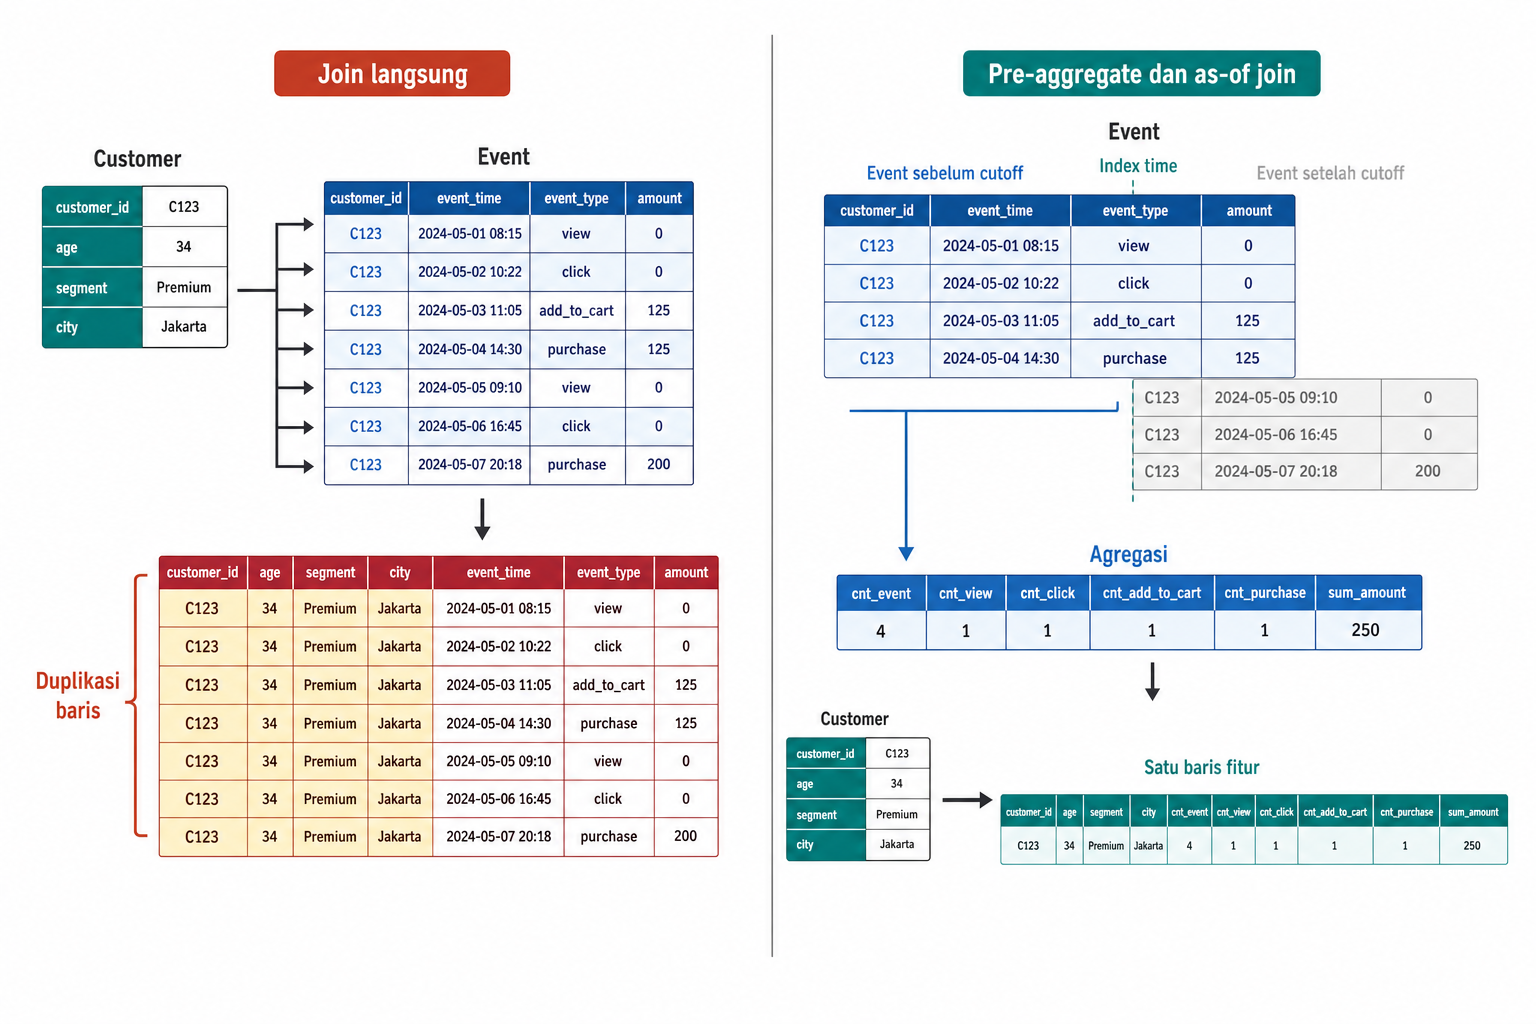
\includegraphics[width=\linewidth,height=0.72\textheight,keepaspectratio]{ch06-fig-3}
\caption{Perbandingan Antara Join Standar dengan As-Of Join}
\label{fig:ch06-fig-3}
\end{figure}

Teknik \emph{as-of join} mencegah kebocoran ini. \emph{As-of join} memasangkan baris ke catatan paling akhir di tabel log yang waktu kejadiannya lebih tua dari stempel waktu referensi. Mekanisme ini menarik garis potong waktu yang absolut, sehingga agregasi berhenti dengan aman tepat sebelum indeks prediksi.

Pemenuhan kebenaran \emph{point-in-time} mengubah kumpulan log mentah menjadi representasi historis yang aman dari kebocoran. Penguasaan atas teknik ini merupakan prasyarat sebelum merakit kerangka rekayasa fitur otomatis pada data relasional yang akan dibahas pada bab selanjutnya.

\section{Fitur Berbasis Domain: Menyandikan Pengetahuan Pakar}\label{fitur-berbasis-domain-menyandikan-pengetahuan-pakar}

Sinyal prediktif yang kuat sering kali bersumber dari pemahaman spesifik terhadap masalah yang diselesaikan. Fitur berbasis domain adalah terjemahan langsung dari aturan bisnis, standar klinis, atau formula industri ke dalam variabel matematis.

Representasi yang dirancang manusia ini membebaskan model dari beban untuk memetakan logika dasar melalui proses coba-coba. Menyuntikkan pengetahuan pakar secara eksplisit ke dalam \emph{dataset} memberikan beberapa keuntungan operasional:

\begin{enumerate}
\def\labelenumi{\arabic{enumi}.}
\tightlist
\item
  \textbf{Mempercepat konvergensi:} Model langsung menerima sinyal matang, memangkas waktu komputasi untuk mencari hubungan antarvariabel dari nol.
\item
  \textbf{Mengurangi korelasi semu:} Rumus yang teruji oleh pakar lebih kebal terhadap \emph{noise} dibandingkan pola yang ditemukan secara acak oleh algoritma.
\item
  \textbf{Menjaga validitas:} Keputusan model tetap sejalan dengan pedoman keilmuan atau praktik komersial yang berlaku di dunia nyata.
\end{enumerate}

Penerapan fitur berbasis domain sangat bervariasi bergantung pada sektor industri yang ditangani.

\textbf{Kesehatan dan Medis}
Dalam prediksi risiko kesehatan, praktisi medis mengevaluasi proporsi tubuh menggunakan Indeks Massa Tubuh (BMI):

\[ \text{BMI} = \frac{w}{h^2} \]

Di mana \(w\) mewakili berat badan (kilogram) dan \(h\) mewakili tinggi badan (meter). Menyediakan BMI sebagai fitur memastikan model langsung menangkap interaksi non-linier antara kedua variabel tersebut. Pada skala perawatan intensif, rekayasa fitur domain berwujud skor komposit seperti APACHE (\emph{Acute Physiology And Chronic Health Evaluation}) atau SOFA (\emph{Sequential Organ Failure Assessment}), yang secara sistematis menggabungkan belasan tanda vital mentah menjadi satu metrik tingkat keparahan.

\textbf{Finansial dan Perbankan}
Analis kredit tidak mengevaluasi pinjaman hanya dengan melihat total pendapatan mentah. Mereka menggunakan formula penilaian risiko yang telah mapan.

\begin{figure}[htbp]\centering
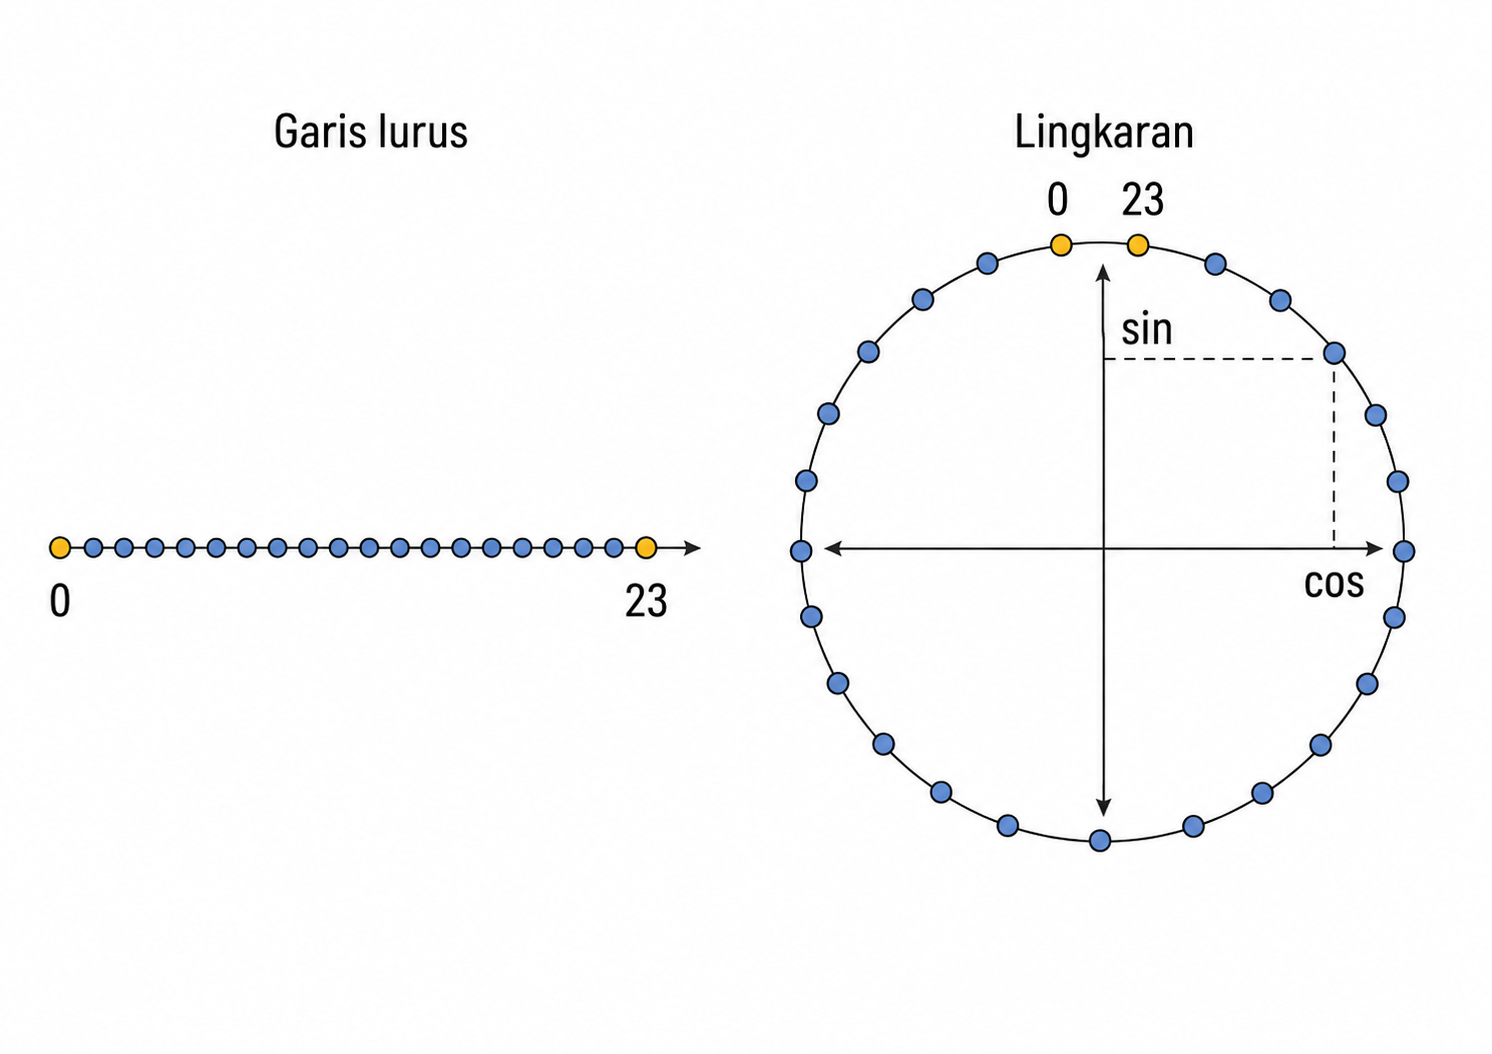
\includegraphics[width=\linewidth,height=0.72\textheight,keepaspectratio]{ch06-fig-4}
\caption{Alur Transformasi Variabel Neraca Menjadi Fitur Risiko Komposit Altman Z-Score}
\label{fig:ch06-fig-4}
\end{figure}

Praktik rekayasa fitur di domain keuangan meliputi:

\begin{enumerate}
\def\labelenumi{\arabic{enumi}.}
\tightlist
\item
  \textbf{Rasio profil risiko:} \emph{Loan-to-value} (LTV) atau \emph{debt-service coverage ratio} (DSCR) untuk mengukur kapasitas bayar pelanggan secara proporsional.
\item
  \textbf{Indikator teknikal:} RSI (\emph{Relative Strength Index}) dan MACD (\emph{Moving Average Convergence Divergence}) yang diturunkan dari data pasar historis seperti pembukaan, penutupan, dan volume (OHLCV).
\item
  \textbf{Indeks prediktif:} Altman Z-score, yakni kombinasi linier dari lima rasio neraca keuangan berbeda untuk mengestimasi risiko kebangkrutan suatu entitas bisnis.
\end{enumerate}

\textbf{Analitik Edukasi (\emph{Learning Analytics})}
Pada sistem pembelajaran digital, log aktivitas mahasiswa diubah menjadi metrik yang mencerminkan pola belajar. Fitur turunan ini mencakup total waktu pengerjaan modul (\emph{time-on-task}), jumlah percobaan sebelum memberikan jawaban benar, hingga jeda waktu antar-sesi. Kompilasi fitur ini menghasilkan metrik keterlibatan yang jauh lebih representatif dibandingkan sekadar menghitung frekuensi \emph{login}.

\section{Fitur Waktu dan Siklik}\label{fitur-waktu-dan-siklik}

Data stempel waktu (\emph{timestamp}) mentah biasanya direkam sebagai deretan angka yang terus membesar, seperti nilai detik UNIX. Jika data ini dimasukkan langsung, model hanya melihat garis lurus yang naik. Format ini gagal menangkap pola perilaku berulang yang terikat dengan ritme aktivitas manusia. Agar dapat dimanfaatkan, stempel waktu tersebut perlu diurai menjadi komponen-komponen diskrit.

\textbf{Ekstraksi Komponen Kalender.}\label{ekstraksi-komponen-kalender}

Langkah pertama yang umum dilakukan adalah memecah waktu menjadi atribut kalender. Dari satu nilai stempel waktu, kita dapat menurunkan berbagai fitur turunan melalui beberapa kategori:

\begin{enumerate}
\def\labelenumi{\arabic{enumi}.}
\tightlist
\item
  \textbf{Unit waktu:} Jam kejadian, hari dalam satu minggu, bulan, atau kuartal.
\item
  \textbf{Penanda biner:} Indikator hari libur nasional, akhir pekan, atau jam operasional kerja.
\item
  \textbf{Jarak temporal:} Jumlah hari sejak peristiwa terakhir, atau selisih hari menjelang tenggat waktu.
\end{enumerate}

Pustaka modern seperti \passthrough{\lstinline!Feature-engine!} (melalui modul \passthrough{\lstinline!DatetimeFeatures!}) mampu mengekstrak komponen-komponen ini secara otomatis di dalam \emph{pipeline}. Pembentukan atribut kalender membantu model memetakan rutinitas harian atau mingguan yang memengaruhi data secara langsung, seperti lonjakan kemacetan pada hari kerja atau tren ritel pada akhir pekan.

\textbf{Masalah Jarak pada Waktu Linier.}\label{masalah-jarak-pada-waktu-linier}

Pemisahan komponen kalender memunculkan isu matematis baru terkait perhitungan jarak. Waktu memiliki sifat siklik atau berputar:

\begin{enumerate}
\def\labelenumi{\arabic{enumi}.}
\tightlist
\item
  Bulan Desember (12) berdekatan langsung dengan bulan Januari (1).
\item
  Pukul 23.00 malam hanya berjarak satu jam dari pukul 00.00 dini hari.
\end{enumerate}

Jika waktu dibiarkan tersaji sebagai bilangan bulat linear dari 0 hingga 23, model yang bekerja berdasarkan metrik jarak (seperti K-NN atau regresi) akan mengira bahwa angka 0 dan 23 saling berjauhan. Kesalahan evaluasi ini merusak pemahaman algoritma terhadap peristiwa yang terjadi melintasi pergantian siklus.

\textbf{Transformasi Siklik dengan Trigonometri.}\label{transformasi-siklik-dengan-trigonometri}

Untuk mempertahankan bentuk asli waktu, representasi linear dikonversi melalui \emph{encoding} siklik. Sumbu waktu dibengkokkan menjadi lingkaran menggunakan fungsi trigonometri, sehingga satu variabel waktu diproyeksikan menjadi dua komponen terpisah:

\[ x_{\text{sin}} = \sin\left(\frac{2\pi \cdot x}{\max(x)}\right) \]

\[ x_{\text{cos}} = \cos\left(\frac{2\pi \cdot x}{\max(x)}\right) \]

Pada persamaan tersebut, \(x\) mewakili nilai waktu asli (misalnya, pukul 23), sedangkan \(\max(x)\) adalah batas rentang atas pada siklus tersebut (misalnya, 24 untuk skala jam, atau 12 untuk bulan).

\begin{figure}[htbp]\centering
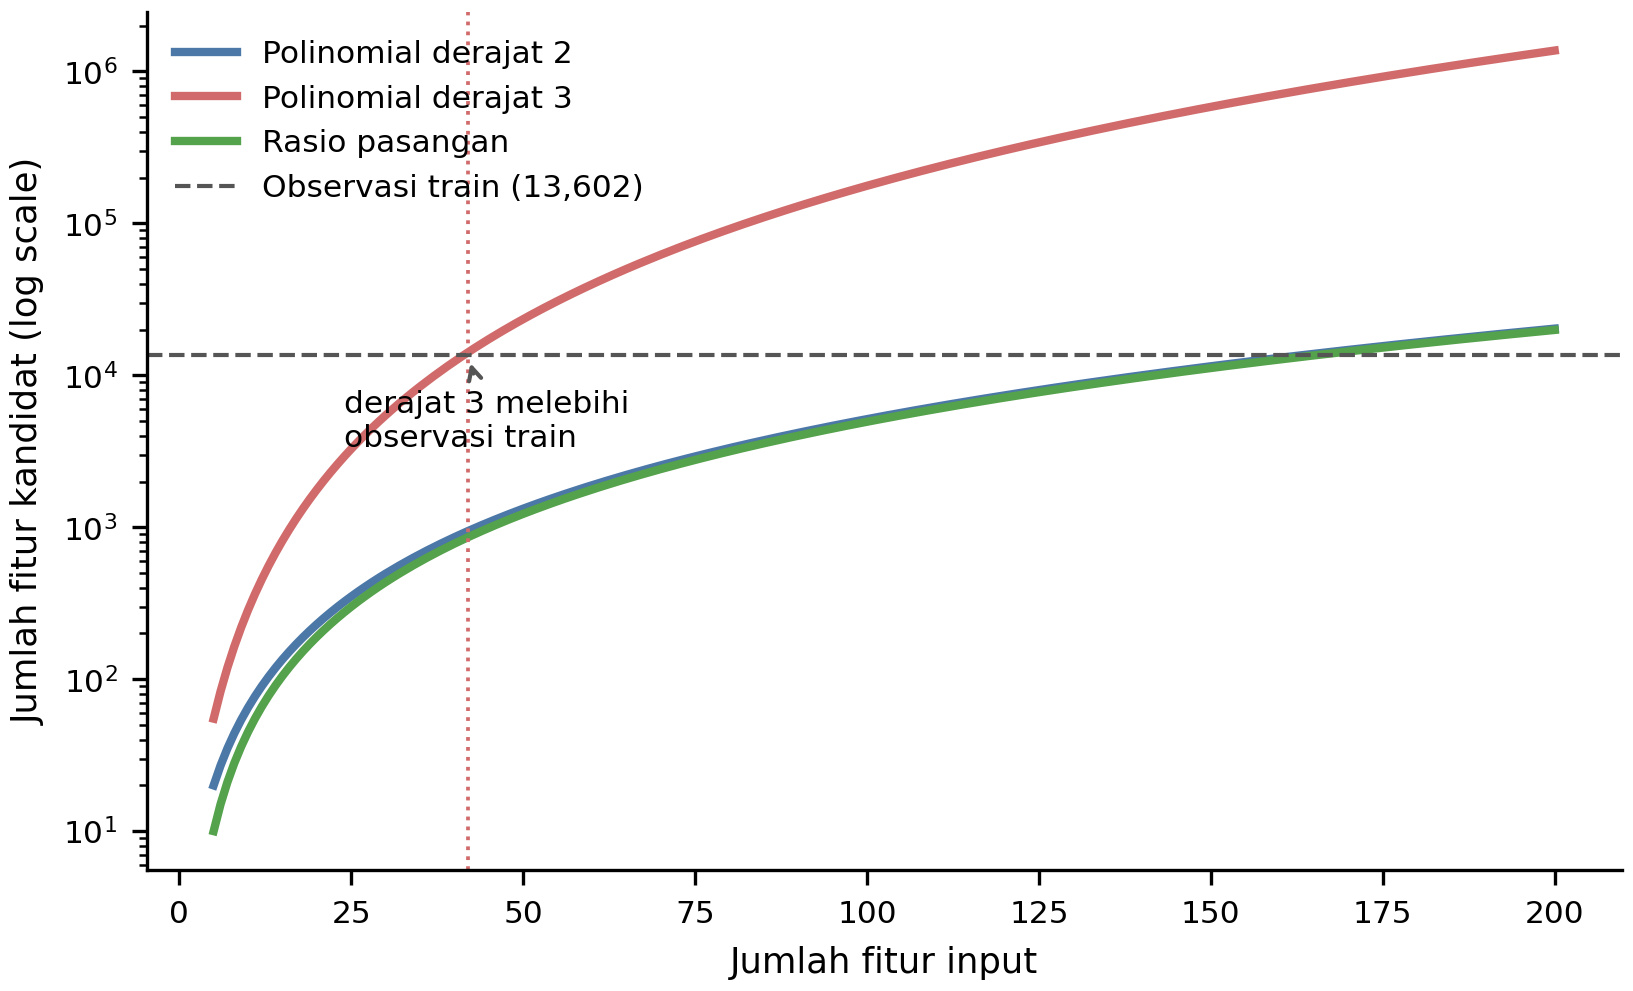
\includegraphics[width=\linewidth,height=0.72\textheight,keepaspectratio]{ch06-fig-5}
\caption{Transformasi Siklik yang Memetakan Nilai Jam dari 0-23 ke dalam Lingkaran 2D (Sin, Cos)}
\label{fig:ch06-fig-5}
\end{figure}

Gambar 6.6 mengilustrasikan bagaimana \emph{encoding} siklik memetakan waktu ke ruang dua dimensi. Nilai jam kini direpresentasikan sebagai pasangan koordinat \((x_{\text{sin}}, x_{\text{cos}})\). Transformasi ini menjamin bahwa jarak antara titik akhir siklus dan titik awal berikutnya tetap berdekatan. Dalam praktiknya, konversi matematis ini sering kali difasilitasi oleh transformer seperti \passthrough{\lstinline!CyclicalFeatures!} (yang dapat menghapus kolom linear asalnya), memastikan ruang vektor fitur beroperasi dengan benar baik pada fase pelatihan maupun inferensi.

\section{Risiko Ledakan Fitur}\label{risiko-ledakan-fitur}

Rekayasa fitur sering dipahami secara keliru sebagai proses memperbanyak kolom data tanpa batas. Perangkat lunak saat ini sangat memudahkan proses penciptaan ribuan turunan melalui operasi matematis otomatis, seperti polinomial, interaksi antarvariabel, dan agregasi grup. Namun, ekspansi variabel yang dibiarkan tanpa kendali justru merusak struktur \emph{dataset}. Fenomena ini dikenal sebagai ledakan fitur (\emph{feature explosion}).

\begin{figure}[htbp]\centering
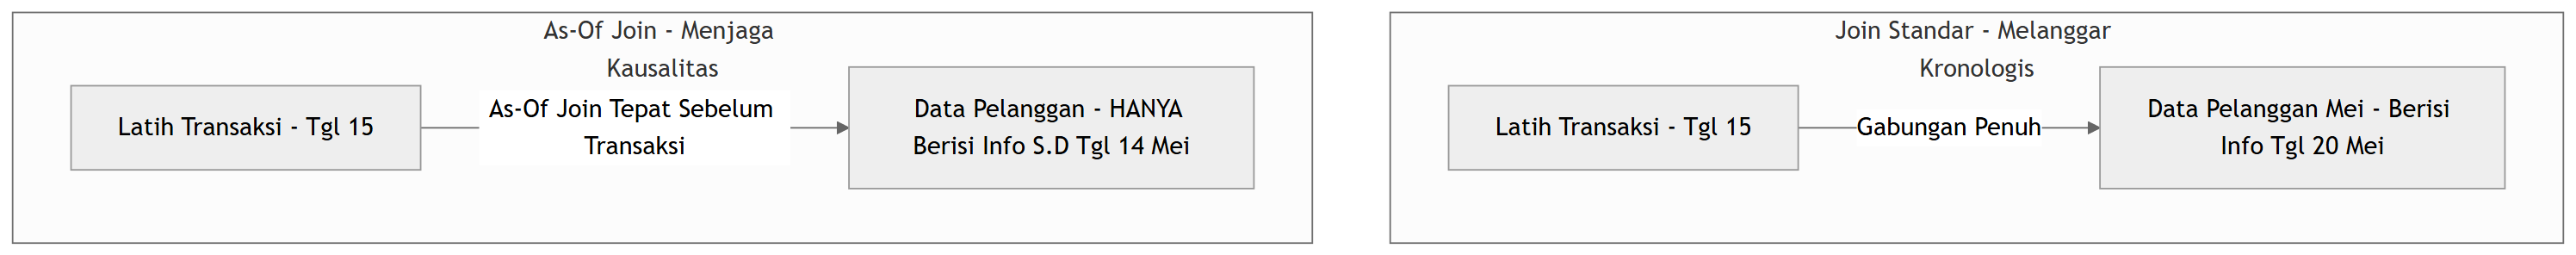
\includegraphics[width=\linewidth,height=0.72\textheight,keepaspectratio]{ch06-fig-6}
\caption{Diagram Evaluasi Akurasi Model Baseline Melawan Model Berfitur Turunan pada CV}
\label{fig:ch06-fig-6}
\end{figure}

Membesarkan dimensi data secara kombinatorial tanpa landasan teori mendatangkan tiga masalah komputasi utama:

\begin{enumerate}
\def\labelenumi{\arabic{enumi}.}
\tightlist
\item
  \textbf{Dominasi \emph{noise}:} Sebagai ilustrasi matematis, membangun seluruh rasio dari 100 fitur dasar secara langsung menghasilkan hampir 10.000 fitur baru. Mayoritas kolom tambahan ini hanya berupa \emph{noise} murni dan gagal memberikan sinyal komputasi yang valid bagi model.
\item
  \textbf{Kutukan dimensi:} Penambahan dimensi baru memperbesar volume ruang fitur secara eksponensial. Titik-titik observasi saling menjauh dan tersebar sangat renggang. Kondisi ini menyulitkan pemetaan batas pemisah. Model rentan mengalami \emph{overfitting} karena algoritma cenderung menghafal \emph{noise} dari data pelatihan.
\item
  \textbf{Kelumpuhan komputasi:} Arsitektur prediktif berbasis pohon keputusan memang lebih kebal terhadap variabel acak. Walaupun demikian, struktur algoritmanya tetap harus menanggung beban berat saat memilah ribuan cabang tambahan. Fase pelatihan membutuhkan durasi yang lebih panjang and memakan alokasi memori secara masif tanpa jaminan peningkatan akurasi.
\end{enumerate}

Penumpukan turunan variabel matematis juga berpotensi menciptakan multikolinearitas. Kondisi ini muncul ketika beberapa variabel prediktor saling memuat sinyal yang tumpang tindih. Redundansi observasi merusak cara kerja algoritma parametrik (seperti regresi linear) karena estimasi bobot koefisien kehilangan stabilitas.

Kita dapat mendeteksi tingkat keparahan multikolinearitas menggunakan \emph{Variance Inflation Factor} (VIF).

\[ VIF_i = \frac{1}{1 - R_i^2} \]

Di mana \(R_i^2\) merupakan koefisien determinasi saat fitur \(x_i\) diregresikan terhadap semua fitur lain di dalam \emph{dataset}. Nilai VIF melebihi angka 5 atau 10 menandakan sebuah fitur berkorelasi terlalu kuat dengan prediktor lain dan layak dihapus.

Kita harus mengombinasikan pembuatan turunan matematis dengan pemangkasan sistematis untuk memitigasi risiko ledakan fitur. Praktik rekayasa fitur modern menangani dimensi berlebih melalui pendekatan berikut:

\begin{enumerate}
\def\labelenumi{\arabic{enumi}.}
\tightlist
\item
  \textbf{Pemangkasan korelasi:} Membuang fitur turunan menggunakan penyaringan berbasis nilai VIF atau ambang batas korelasi berpasangan.
\item
  \textbf{Regularisasi L1 (Lasso):} Menerapkan penalti saat proses pelatihan berlangsung untuk menekan bobot koefisien fitur yang redundan menjadi nol secara otomatis.
\item
  \textbf{Penyaringan pra-kombinasi:} Mengukur signifikansi interaksi melalui metode statistik (seperti uji ANOVA) sebelum mengeksekusi ekspansi polinomial. Langkah ini mencegah penggabungan fitur-fitur yang sejak awal sudah lemah.
\end{enumerate}

Penciptaan atribut matematis yang baru mutlak memerlukan pijakan teori yang kuat. Kita mendefinisikan representasi baru semata-mata untuk memandu model mengenali pola faktual. Argumen komputasi dan praktik pembuktian empiris ini menjadi landasan saat mendalami metodologi seleksi fitur di Bab 7 dan mekanisme evaluasi model di Bab 9.

\section{Memvalidasi Manfaat Fitur Turunan Baru}\label{memvalidasi-manfaat-fitur-turunan-baru}

Pembentukan fitur turunan selalu berawal dari hipotesis empiris. Saat kita menggabungkan beberapa atribut, kita berasumsi interaksi tersebut akan memperjelas pola spesifik di dalam data. Fitur turunan yang secara logika masuk akal bagi pemahaman manusia belum tentu memberi utilitas prediktif tambahan bagi model. Beberapa jenis algoritma sudah dapat mengekstrak informasi yang sama langsung dari kumpulan data mentahnya.

Mempertahankan atribut yang redundan memperlebar dimensi data secara sia-sia. Matriks fitur yang membengkak berisiko mengumpulkan \emph{noise}, membebani memori komputasi, dan memicu kondisi \emph{overfitting}. Algoritma menggunakan kapasitasnya untuk menghafal kombinasi nilai spesifik pada data latih, lalu gagal menggeneralisasi polanya saat memproses observasi baru.

\textbf{Perbandingan terhadap Baseline.}\label{perbandingan-terhadap-baseline}

Validasi kelayakan atribut turunan membutuhkan model \emph{baseline}. Model referensi ini dilatih hanya menggunakan fitur mentah awal. Kualitas fitur baru tidak dapat dinilai memakai nilai galat latih. Menambahkan dimensi ke dalam matriks data hampir selalu mengurangi galat latih dan menciptakan ilusi akurasi yang menyesatkan.

Setiap pengujian atribut wajib didasarkan pada skema \emph{cross-validation} guna mengukur performa di atas set data terisolasi.

\[ CV_{\text{score}} = \frac{1}{K} \sum_{k=1}^{K} \text{Metrik}(y_{\text{val}}^{(k)}, \hat{y}_{\text{val}}^{(k)}) \]

Di mana \(K\) merupakan jumlah lipatan (\emph{fold}) pengujian, \(y_{\text{val}}^{(k)}\) adalah vektor target aktual pada lipatan ke-\(k\), dan \(\hat{y}_{\text{val}}^{(k)}\) adalah keluaran prediksi dari model. Skor \(CV_{\text{score}}\) dari model berfitur turunan harus melampaui skor \emph{baseline} secara stabil di seluruh lipatan data. Jika tidak ada margin peningkatan yang jelas, fitur turunan baru tersebut harus dieliminasi.

\begin{figure}[htbp]\centering
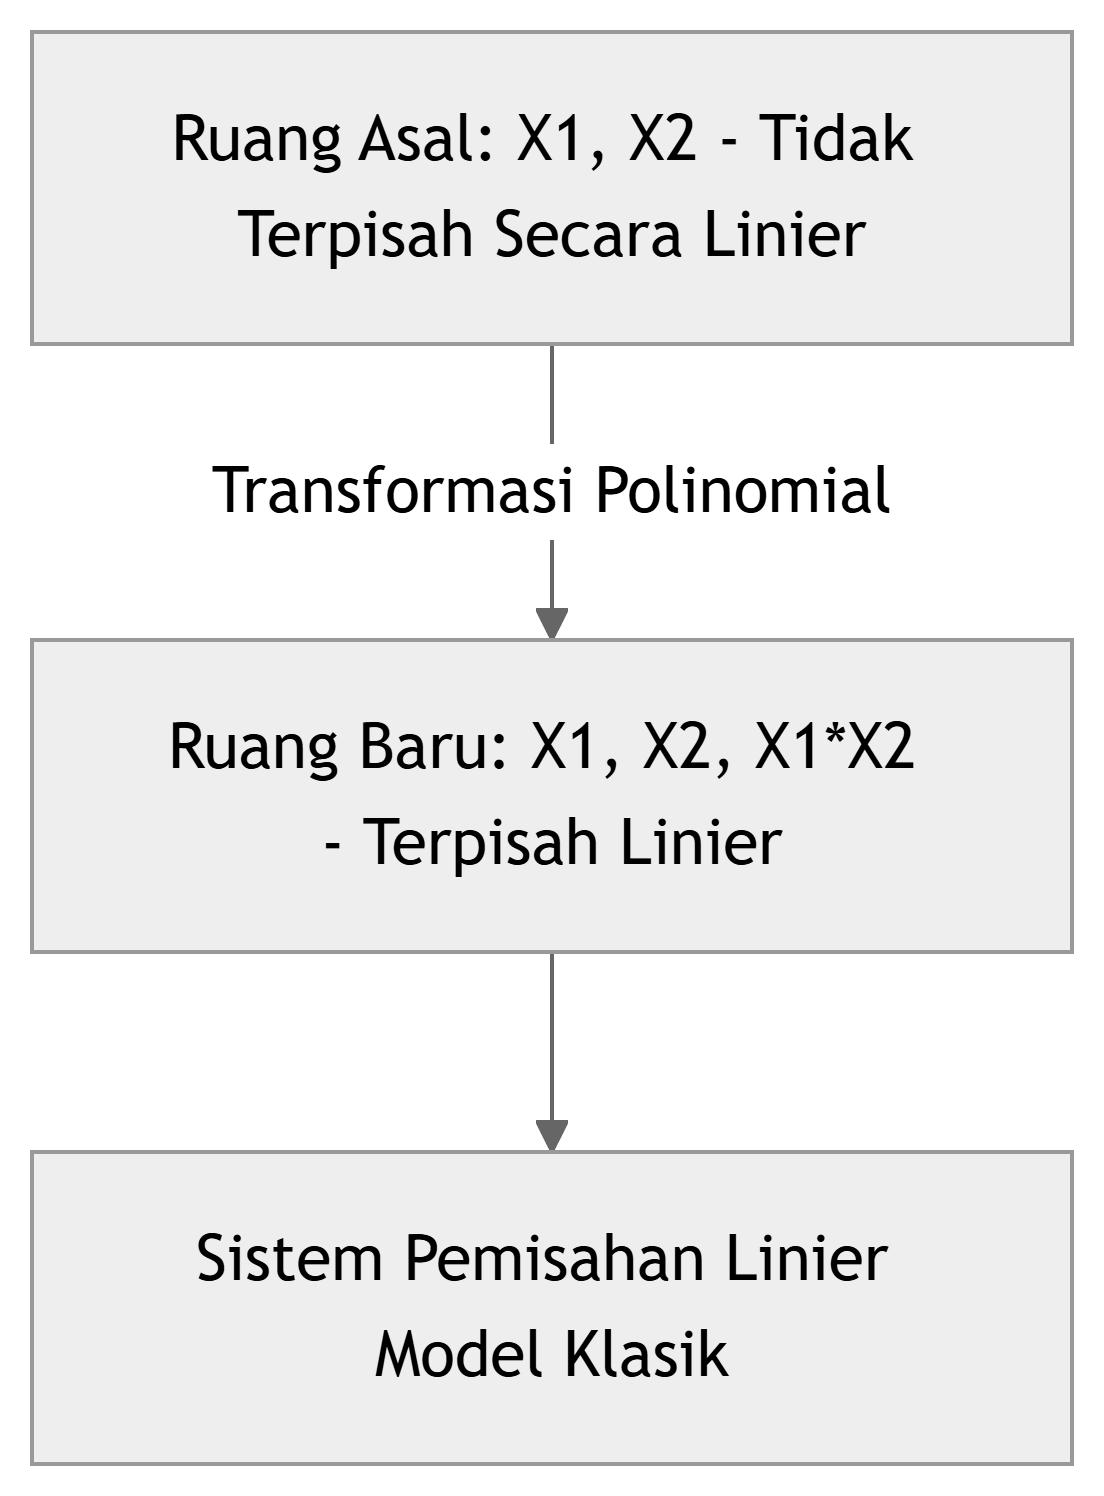
\includegraphics[width=\linewidth,height=0.72\textheight,keepaspectratio]{ch06-fig-7}
\caption{Representasi Rasio Finansial dari Agregasi Log Peristiwa}
\label{fig:ch06-fig-7}
\end{figure}

\textbf{Metode Diagnostik Lanjutan.}\label{metode-diagnostik-lanjutan}

Selain mengandalkan akurasi metrik agregat, arsitektur representasi dapat dievaluasi memakai metode diagnostik lanjutan untuk memahami kontribusi fitur secara spesifik:

\begin{enumerate}
\def\labelenumi{\arabic{enumi}.}
\tightlist
\item
  \textbf{Studi Ablasio Kelompok (\emph{Group Ablation Study}):} Teknik ini mengelompokkan atribut turunan berdasarkan jenisnya, misalnya kelompok rasio matematis atau agregasi temporal. Evaluasi performa dilakukan dengan menghapus kelompok-kelompok tersebut satu per satu. Pendekatan ini memperlihatkan kategori transformasi mana yang menyumbang sinyal murni.
\item
  \textbf{Seleksi Fitur \emph{Probe} (\emph{Probe Feature Selection}):} Analis menyisipkan satu kolom derau acak ke dalam matriks data latih. Semua fitur turunan yang menghasilkan skor \emph{feature importance} lebih rendah dari atribut \emph{probe} ini terbukti beroperasi pada level acak dan otomatis dibuang.
\item
  \textbf{Diagnosis Kontribusi SHAP:} Metode analisis prediksi ini mendekomposisi bobot utilitas tiap dimensi matriks. Jika suatu atribut turunan sekadar mengambil alih porsi nilai SHAP dari fitur mentah pembentuknya tanpa mendongkrak skor metrik keseluruhan, fitur turunan tersebut tergolong berlebih.
\end{enumerate}

Bab 9 membahas metode evaluasi fitur secara menyeluruh. Pada tahap awal rekayasa data, prinsip dasarnya harus ditaati: fungsi turunan memperbesar ukuran matriks komputasi, dan eksistensinya hanya valid setelah lulus pengujian empiris.

\section{Studi Kasus: Fitur Turunan pada Data Transaksi, Kesehatan, dan Pendidikan}\label{studi-kasus-fitur-turunan-pada-data-transaksi-kesehatan-dan-pendidikan}

Pengetahuan domain merupakan fondasi intelektual utama dalam rekayasa fitur turunan. Fitur prediktif yang andal berakar dari pemahaman logis tentang mekanisme di dunia nyata. Tiga bidang empiris berikut mengilustrasikan bagaimana wawasan industri mengarahkan transformasi dari atribut mentah menjadi representasi model yang spesifik.

\textbf{1. Data Transaksi Perbankan dan E-commerce}
Tabel data asal biasanya berwujud log peristiwa (\emph{event log}) berupa angka nominal pengeluaran dan stempel waktu tunggal. Menganalisis setiap transaksi secara terisolasi sering kali tidak efektif. Pengetahuan kebiasaan finansial mendorong rekayasawan untuk merancang fitur agregasi temporal, seperti kalkulasi rata-rata pengeluaran berbobot kebaruan (\emph{recency-weighted mean}) selama tiga puluh hari terakhir. Praktisi juga memformulasikan metrik rasio, misalnya persentase transaksi silang terhadap profil pendapatan. Otomasi tingkat lanjut dapat dicapai menggunakan pustaka seperti \emph{tsfresh} yang mampu mengekstraksi ratusan fitur runtun waktu sekaligus (statistik, spektral, entropi) dari log transaksi.

\textbf{2. Rekam Medis dan Kesehatan}
Formulir rekam medis sering kali mencatat variabel biologis secara terpisah. Pengetahuan klinis dapat diterjemahkan menjadi interaksi matematis yang bermakna bagi algoritma \emph{machine learning}:

\begin{enumerate}
\def\labelenumi{\arabic{enumi}.}
\tightlist
\item
  \textbf{Sintesis Domain:} Mentransformasikan parameter dasar tinggi dan berat badan menjadi satu fitur komposisi terpusat, yaitu Indeks Massa Tubuh (BMI). Representasi ini dihitung secara matematis menggunakan rumus:
  \[ \text{BMI} = \frac{\text{Berat Badan (kg)}}{(\text{Tinggi Badan (m)})^2} \]
  Di mana hasil perhitungan ini (BMI) memiliki korelasi klinis yang jauh lebih kuat terhadap risiko penyakit kardiovaskular dibandingkan jika model hanya mempelajari fitur bobot atau tinggi secara individual.
\item
  \textbf{Delta Pergeseran Historis:} Fitur komparatif yang menyoroti pergeseran nilai kesehatan di antara jadwal observasi sering menyimpan sinyal prediktif tinggi. Menghitung nilai selisih tekanan darah kunjungan saat ini dengan kunjungan sebelumnya akan menghasilkan fitur lintasan medis (progres kondisi pasien) yang lebih kaya informasi ketimbang status absolut.
\end{enumerate}

\textbf{3. Sistem Manajemen Pendidikan Digital}
Sistem pendidikan menghasilkan ribuan log aktivitas masuk (\emph{login}) dan statistik ujian. Namun, teori pedagogi menetapkan bahwa keteraturan belajar mencerminkan komitmen siswa dengan lebih konsisten dibandingkan sekadar menjumlahkan frekuensi klik. Oleh karena itu, fitur dikembangkan melalui:

\begin{enumerate}
\def\labelenumi{\arabic{enumi}.}
\tightlist
\item
  \textbf{Sintesis Keteraturan:} Menghitung jumlah hari \emph{login} beruntun tanpa jeda (\emph{streak}) sebagai indikator motivasi belajar.
\item
  \textbf{Rasio Penyelesaian:} Perbandingan proporsional antara tugas yang dirampungkan dengan akumulasi sisa kuota penugasan.
\end{enumerate}

Melalui intervensi yang dituntun oleh wawasan teori, rekayasa fitur bertugas menerjemahkan volume catatan log yang masif menjadi sekumpulan sinyal perilaku yang terstruktur, padat, dan langsung relevan bagi algoritma pemodelan sasaran.

% ==========================================================================
% ch07.tex — dihasilkan dari v2/drafts oleh tools/md2tex.py
% Sumber: v2\drafts\ch07\ch07_draft_v2.md
% Boleh disunting manual; menjalankan md2tex.py lagi akan menimpa.
% ==========================================================================
\chapter{Seleksi Fitur}\label{seleksi-fitur}

Representasi yang terlalu lebar tidak selalu lebih informatif. Banyak kolom yang bergerak bersama karena berasal dari sumber yang sama, sedangkan kolom lain hanya membawa \emph{noise}. Pada data berdimensi tinggi, model lebih mudah menghafal daripada belajar pola yang menggeneralisasi. Pada sistem produksi, setiap fitur yang dipertahankan harus dihitung, dimonitor, dan dijaga definisinya. Karena itu, seleksi fitur diperlukan untuk menyimpan informasi berguna sambil mengurangi \emph{noise}, redundansi, biaya komputasi, dan kesulitan interpretasi.

Tiga keluarga metode dibahas dalam bab ini. Metode filter menilai fitur dengan statistik sebelum model dilatih, cepat tetapi buta terhadap interaksi. Metode wrapper memilih subset dengan melatih dan mengevaluasi model, kuat tetapi mahal. Metode embedded melakukan seleksi selama pelatihan, misalnya melalui penalti L1. Bab ini menguraikan ketiga keluarga tersebut serta menekankan bahwa seleksi fitur harus berada di dalam alur validasi, bukan dilakukan sekali pada seluruh dataset sebelum evaluasi.

\section{\texorpdfstring{Relevansi, Redundansi, dan \emph{Curse of Dimensionality}}{Relevansi, Redundansi, dan Curse of Dimensionality}}\label{relevansi-redundansi-dan-curse-of-dimensionality}

Sebuah fitur disebut relevan jika fitur tersebut membawa informasi yang berguna untuk target pada tugas tertentu. Pada dataset Breast Cancer Wisconsin Diagnostic (WDBC), \emph{worst concave points} atau \emph{worst radius} dapat membantu membedakan diagnosis karena terkait dengan bentuk inti sel. Sebaliknya, fitur \emph{probe-noise} seharusnya tidak konsisten membantu. Relevansi selalu melekat pada tugas, sehingga fitur yang penting untuk satu target bisa tidak berguna untuk target lain.

Redundansi berbeda dari ketidakrelevanan. Fitur redundan bisa relevan, tetapi informasinya sudah diwakili oleh fitur lain. Pada WDBC, radius, perimeter, dan area tidak identik, tetapi ketiganya membawa informasi ukuran sel yang sangat berkaitan. \emph{Mean radius} dan \emph{mean perimeter} dapat sama-sama relevan untuk diagnosis, namun salah satunya mungkin hanya menambah sedikit informasi setelah yang lain masuk. Karena itu, subset fitur perlu dipahami sebagai tim, bukan daftar pemenang satu per satu.

Seleksi fitur yang ideal mencari himpunan dengan relevansi tinggi terhadap target dan redundansi rendah antaranggota (Guyon and Elisseeff 2003). Prinsip ini muncul pada pendekatan seperti minimum-redundancy maximum-relevance, atau mRMR. Intuisinya sederhana. Kita tidak hanya mencari fitur yang kuat sendirian. Kita mencari beberapa fitur yang saling melengkapi.

Dimensi tinggi membuat persoalan tersebut lebih tajam. Semakin banyak fitur, semakin besar risiko \emph{overfitting}, kebutuhan memori, biaya komputasi, dan kesulitan interpretasi. Pada data dengan sampel terbatas, fitur lemah, redundan, atau sengaja dibuat sebagai \emph{probe-noise} dapat mengaburkan sinyal utama. Model mungkin menemukan pola kebetulan yang tidak muncul lagi pada data baru.

\emph{Curse of dimensionality} membuat sampel makin jarang karena volume ruang fitur tumbuh cepat. Jumlah observasi yang dibutuhkan untuk mempertahankan kepadatan data pun dapat meningkat secara eksponensial. Penalaran berbasis jarak ikut memburuk karena tetangga terdekat tidak lagi terasa jauh lebih dekat dibanding titik lain. Seleksi fitur mengurangi sebagian beban ini dengan menghapus dimensi yang tidak perlu. Bab 8 mengambil jalur lain, yaitu mengompresi fitur ke ruang representasi baru.

Lebih sedikit fitur tidak otomatis berarti lebih baik. Menghapus fitur yang benar-benar membawa sinyal dapat merusak performa dan bahkan kewajaran model. Seleksi fitur yang baik bukan tindakan merapikan tabel, melainkan memilih representasi yang lebih stabil dan lebih mudah digeneralisasi. Dari kerangka relevansi dan redundansi ini, metode yang paling mudah dimulai adalah metode yang memberi skor statistik pada fitur.

\begin{pendalaman}{Konsentrasi jarak di dimensi tinggi}
Ketika dimensi bertambah, selisih antara tetangga terdekat dan terjauh dapat mengecil relatif terhadap jarak itu sendiri. Dengan kata lain, semua titik tampak hampir sama jauhnya. Metode berbasis jarak seperti k-NN, clustering, atau kernel tertentu kehilangan daya pembeda karena struktur kedekatan menjadi kabur. Ini adalah sifat geometri dimensi tinggi, bukan masalah kualitas data saja. Karena itu, menghapus dimensi yang tidak perlu melalui seleksi fitur, atau mengompresinya seperti pada Bab 8, dapat membantu.
\end{pendalaman}

\section{\texorpdfstring{Metode \emph{Filter}}{Metode Filter}}\label{metode-filter}

Cara paling murah untuk menyeleksi fitur adalah menilai setiap fitur sebelum model akhir dilatih. Metode \emph{filter} bekerja seperti gerbang awal. Fitur diberi skor, lalu sebagian dipertahankan berdasarkan ambang, peringkat, atau jumlah fitur yang diinginkan. Contohnya adalah \emph{variance threshold}, korelasi, \emph{chi-square}, ANOVA F-test klasifikasi untuk menilai perbedaan rata-rata fitur numerik antar kelas, serta \emph{mutual information}. Untuk target kontinu, \passthrough{\lstinline!f_regression!} menilai asosiasi linear antara fitur numerik dan target; pertanyaannya berbeda dari perbandingan rata-rata antar kelas.

Gambar 7.1 menempatkan \emph{filter} bersama dua keluarga lain. Pada \emph{filter}, statistik menjadi gerbang sebelum model. Pada \emph{wrapper}, model dilatih berulang kali untuk menilai subset. Pada \emph{embedded}, seleksi terjadi sebagai bagian dari pelatihan model.

\begin{figure}[tbp]\centering
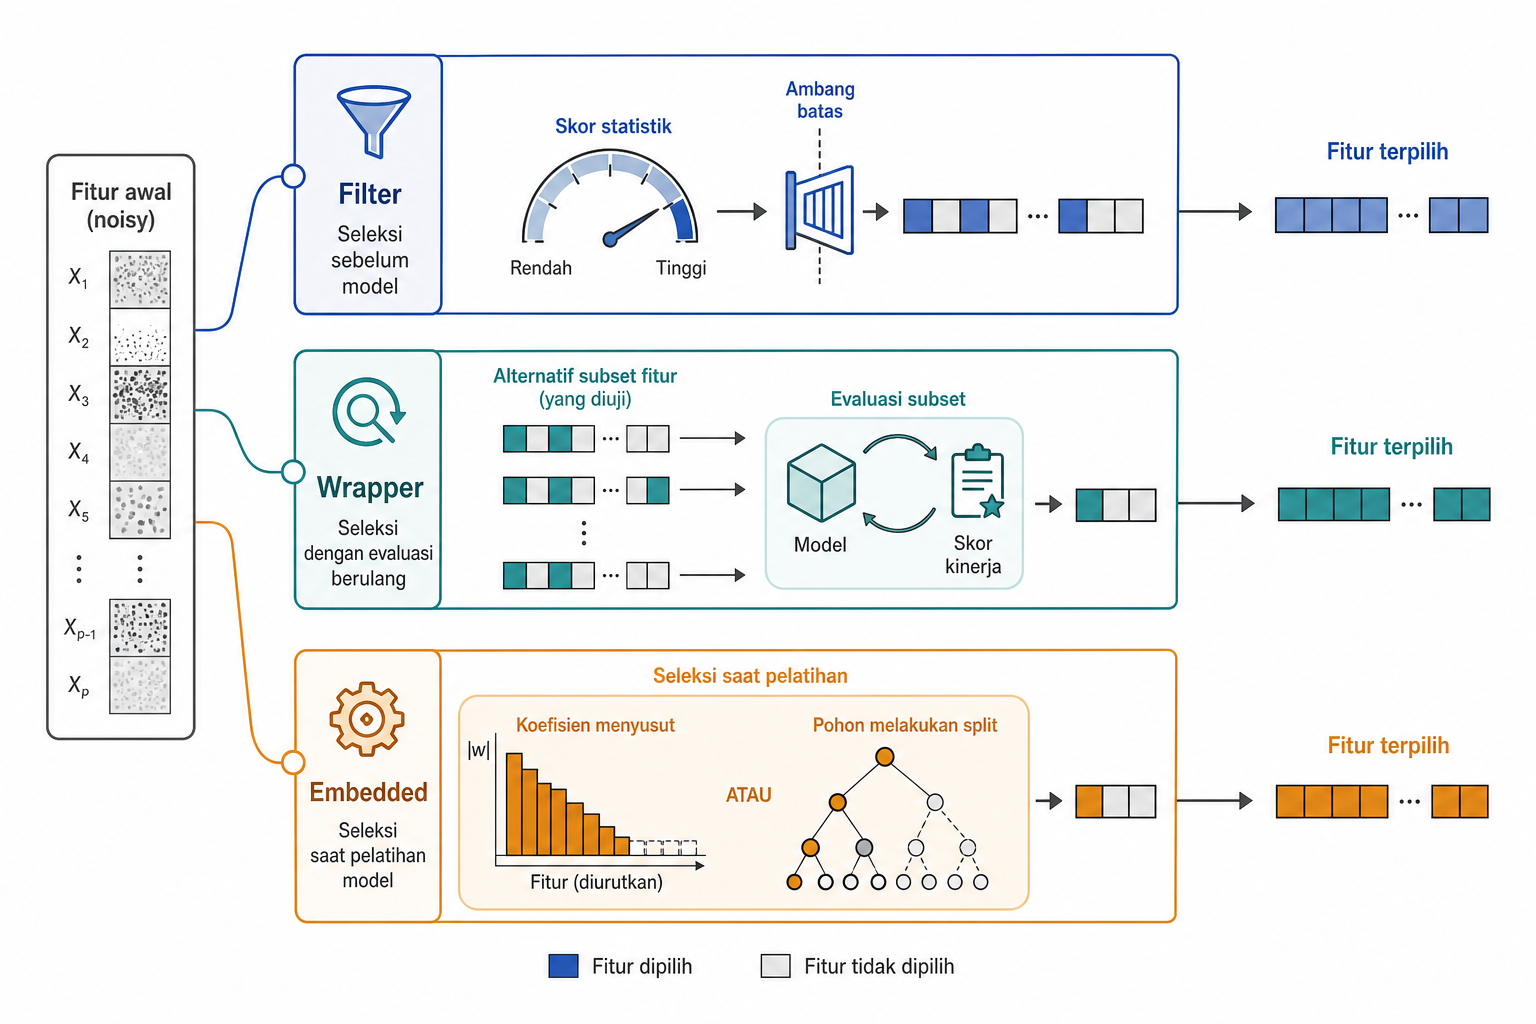
\includegraphics[width=111.6mm]{ch07-fig-1}
\caption{Tiga keluarga metode seleksi fitur}
\label{fig:ch07-fig-1}
\end{figure}

Statistik yang dipakai harus cocok dengan tipe data dan bentuk hubungan yang dicari. Pearson correlation mengukur asosiasi linear antara dua variabel numerik.

\[
r = \dfrac{\sum_i (x_i - \bar{x})(y_i - \bar{y})}{\sqrt{\sum_i (x_i - \bar{x})^2 \sum_i (y_i - \bar{y})^2}}
\]

dengan \(x_i\) dan \(y_i\) sebagai nilai observasi ke-\(i\), sedangkan \(\bar{x}\) dan \(\bar{y}\) adalah rata-ratanya. Korelasi berguna untuk hubungan linear, tetapi dapat gagal pada pola \emph{U-shaped}, hubungan non-linear lain, atau ketika satu \emph{outlier} kuat menarik nilai korelasi.

\emph{Mutual information} mengukur seberapa banyak pengetahuan tentang \(X\) mengurangi ketidakpastian tentang \(Y\).

\[
I(X; Y) = \sum_{x, y} p(x, y) \log \dfrac{p(x, y)}{p(x)\,p(y)}
\]

Karena tidak terbatas pada hubungan linear, \emph{mutual information} dapat menangkap ketergantungan yang lebih umum. \emph{Chi-square} membandingkan frekuensi teramati dan frekuensi harapan di bawah asumsi independensi.

\[
\chi^2 = \sum_i \dfrac{(O_i - E_i)^2}{E_i}
\]

dengan \(O_i\) sebagai frekuensi teramati dan \(E_i\) sebagai frekuensi harapan. Dalam seleksi fitur, \emph{chi-square} cocok untuk fitur bernilai non-negatif, seperti frekuensi atau \emph{count}, dengan target kategorikal.

Kelebihan \emph{filter} adalah kecepatannya. Metode ini berguna sebagai penyaringan awal pada data berdimensi tinggi, misalnya untuk menghapus fitur yang hampir konstan atau memilih fitur teks paling informatif. Keterbatasannya muncul karena banyak \emph{filter} menilai fitur satu per satu. Dua fitur yang lemah sendiri-sendiri mungkin kuat jika muncul bersama, tetapi interaksi semacam itu dapat terlewat. Dua sensor yang hampir identik dapat sama-sama mendapat skor tinggi dan sama-sama lolos.

Seperti \emph{transformer} lain, \emph{filter} harus dipasang di dalam \emph{fold} pelatihan ketika dipakai untuk evaluasi model. Jika skor fitur dihitung dari seluruh \emph{dataset} sebelum \emph{split}, target pada \emph{fold} validasi ikut memengaruhi pilihan fitur. Skor evaluasi menjadi terlalu optimistis. Dalam praktik modern, \emph{attribution score} dari model pohon cepat, misalnya \emph{mean absolute SHAP}, kadang dipakai sebagai \emph{filter} yang lebih sadar model. Tetap saja, langkah ini merupakan proses seleksi dan harus divalidasi. Jika interaksi dan redundansi menjadi terlalu penting untuk diabaikan, seleksi perlu dibuat lebih dekat dengan performa model.

\section{\texorpdfstring{Metode \emph{Wrapper}}{Metode Wrapper}}\label{metode-wrapper}

Metode \emph{wrapper} memilih fitur dengan melatih dan mengevaluasi model pada subset fitur yang berbeda. \emph{Filter} menilai asosiasi setiap fitur dengan target, sedangkan \emph{wrapper} membandingkan subset berdasarkan performa model yang dihasilkan.

Secara ideal, masalahnya dapat ditulis sebagai berikut.

\[
\max_{S \subseteq F} \operatorname{Skor}(M, S)
\]

dengan \(F\) sebagai himpunan semua fitur, \(S\) sebagai subset yang dipilih, \(M\) sebagai model, dan \(\operatorname{Skor}(M, S)\) sebagai performa tervalidasi model memakai subset tersebut. Jika ada \(n\) fitur, jumlah subset yang mungkin adalah \(2^n\). Pencarian lengkap segera menjadi mustahil ketika \(n\) tidak kecil. Karena itu, metode \emph{wrapper} biasanya memakai heuristik \emph{greedy}.

Sequential forward selection mulai dari subset kosong. Pada setiap langkah, metode ini mencoba menambahkan satu fitur yang paling meningkatkan skor. Sequential backward selection mulai dari semua fitur, lalu menghapus satu fitur yang paling sedikit merusak skor. Kedua jalur ini tidak selalu berakhir pada subset yang sama, karena keputusan awal dapat memengaruhi pilihan berikutnya. Karena bersifat \emph{greedy}, metode ini tidak menjamin subset global terbaik.

Gambar 7.2 memperlihatkan dua jalur tersebut pada contoh kecil. Jalur forward tumbuh dari kosong, sedangkan jalur backward menyusut dari set penuh. Di setiap tahap, metode memilih langkah lokal terbaik, bukan menjamin solusi global terbaik.

\begin{figure}[tbp]\centering
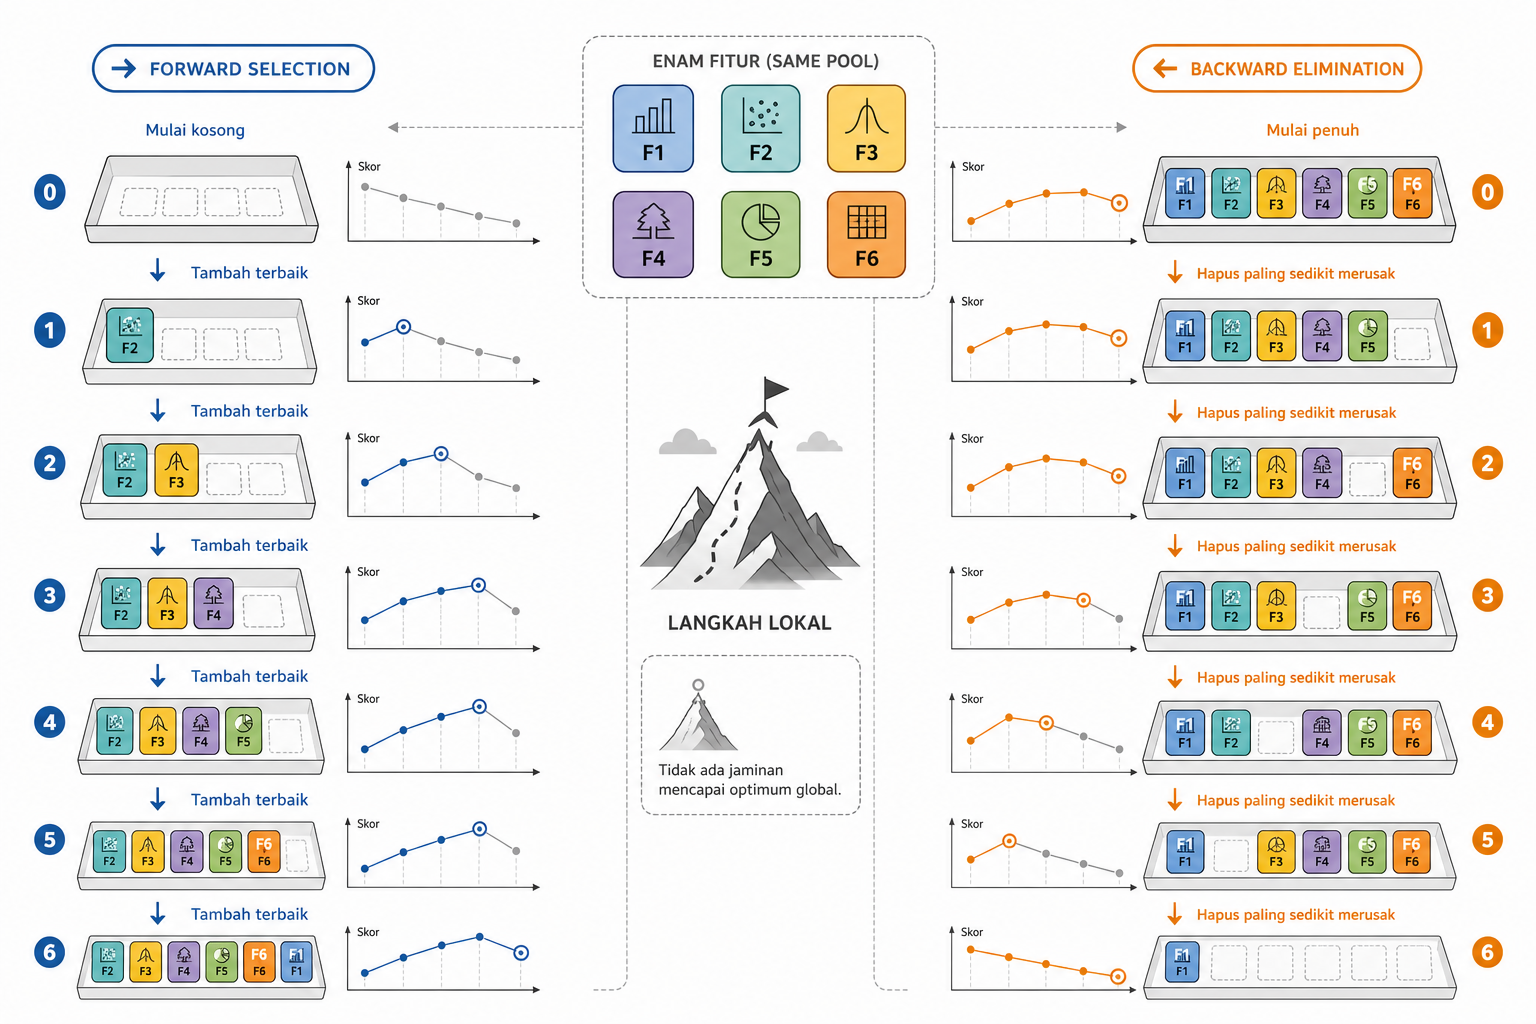
\includegraphics[width=111.6mm]{ch07-fig-2}
\caption{Forward selection dan backward elimination}
\label{fig:ch07-fig-2}
\end{figure}

Recursive feature elimination, atau RFE, mengambil jalur lain. Metode ini melatih model, membaca koefisien atau \emph{feature importance}, menghapus fitur yang dianggap paling lemah, lalu mengulang proses. RFE membutuhkan model yang menyediakan koefisien atau \emph{importance}. Sequential feature selection lebih \emph{model-agnostic} karena hanya membutuhkan skor model pada subset tertentu.

Kelebihan \emph{wrapper} adalah penilaiannya mengikuti model dan metrik yang dipakai. Kemampuannya menangkap interaksi bergantung pada estimator dasar; \emph{wrapper} dengan model linear tanpa fitur interaksi tidak otomatis menemukan hubungan interaktif. Pendekatan ini juga dapat mengurangi redundansi jika model dan metriknya mengenali dua fitur sebagai pengganti. Jika dua fitur hampir saling menyalin, setelah salah satunya masuk ke subset, fitur kedua mungkin tidak lagi menambah skor dan dapat ditinggalkan. Ini berbeda dari \emph{filter} yang sering meloloskan keduanya.

Biayanya adalah komputasi dan risiko \emph{overfitting} terhadap prosedur validasi. Karena model dilatih berkali-kali, \emph{wrapper} mahal pada data besar atau fitur banyak. Pada sampel kecil, subset yang menang bisa saja menang karena kebetulan pada \emph{fold} tertentu. Hasil \emph{wrapper} juga spesifik terhadap model, metrik, dan skema validasi yang dipakai. Fitur yang terpilih untuk model linear belum tentu merupakan fitur terbaik untuk model pohon. Keluarga berikutnya mencoba mengambil sebagian manfaat seleksi yang sadar model tanpa pencarian subset yang terlalu mahal.

\section{\texorpdfstring{Metode \emph{Embedded}}{Metode Embedded}}\label{metode-embedded}

Metode \emph{embedded} mengintegrasikan seleksi ke dalam pelatihan model. Model menghasilkan sinyal seleksi melalui koefisien, regularisasi, atau \emph{feature importance}, sehingga pendekatannya lebih sadar model daripada \emph{filter} dan biasanya lebih ringan daripada pencarian banyak subset pada \emph{wrapper}.

Contoh pentingnya adalah model dengan regularisasi L1, atau LASSO (Tibshirani 1996). Karena WDBC merupakan tugas klasifikasi biner, tujuan yang sesuai untuk contoh ini adalah regresi logistik berpenalti L1.

\[
\min_{w,b} \left[-\dfrac{1}{n}\sum_{i=1}^{n}\left(y_i\log p_i + (1-y_i)\log(1-p_i)\right) + \alpha\lVert w\rVert_1\right],
\qquad p_i = \sigma(w^{\top}x_i+b)
\]

dengan \(y_i \in \{0,1\}\) sebagai label, \(p_i\) sebagai probabilitas kelas positif, \(w\) sebagai vektor bobot, \(b\) sebagai \emph{intercept}, dan \(\alpha\) sebagai pengatur kekuatan penalti. Suku pertama adalah \emph{log loss} klasifikasi, sedangkan suku kedua memberi biaya pada bobot yang tidak nol. Ketika \(\alpha\) dinaikkan, sebagian koefisien dapat didorong sampai tepat nol. Pada fitur yang berkorelasi, L1 dapat memilih salah satu fitur pengganti secara tidak stabil; koefisien nol bukan bukti bahwa fitur lain tidak relevan. Karena penalti bergantung pada skala koefisien, standardisasi harus di-\emph{fit} di dalam setiap \emph{fold} pelatihan.

Gambar 7.3 menggunakan dataset Breast Cancer Wisconsin Diagnostic sebagai contoh kerja untuk memperlihatkan lintasan koefisien saat \(\alpha\) meningkat. Setiap baris mewakili satu sampel massa payudara dengan ciri numerik yang diperoleh dari citra, dan targetnya membedakan diagnosis ganas dengan jinak. Fitur \emph{probe noise} ditambahkan saat percobaan agar penyusutan koefisien terlihat jelas. Sebagian koefisien menyentuh nol lebih awal, sedangkan yang lain bertahan lebih lama; urutan ini bergantung pada kekuatan regularisasi, skala fitur, dan korelasi antarfitur.

\begin{figure}[tbp]\centering
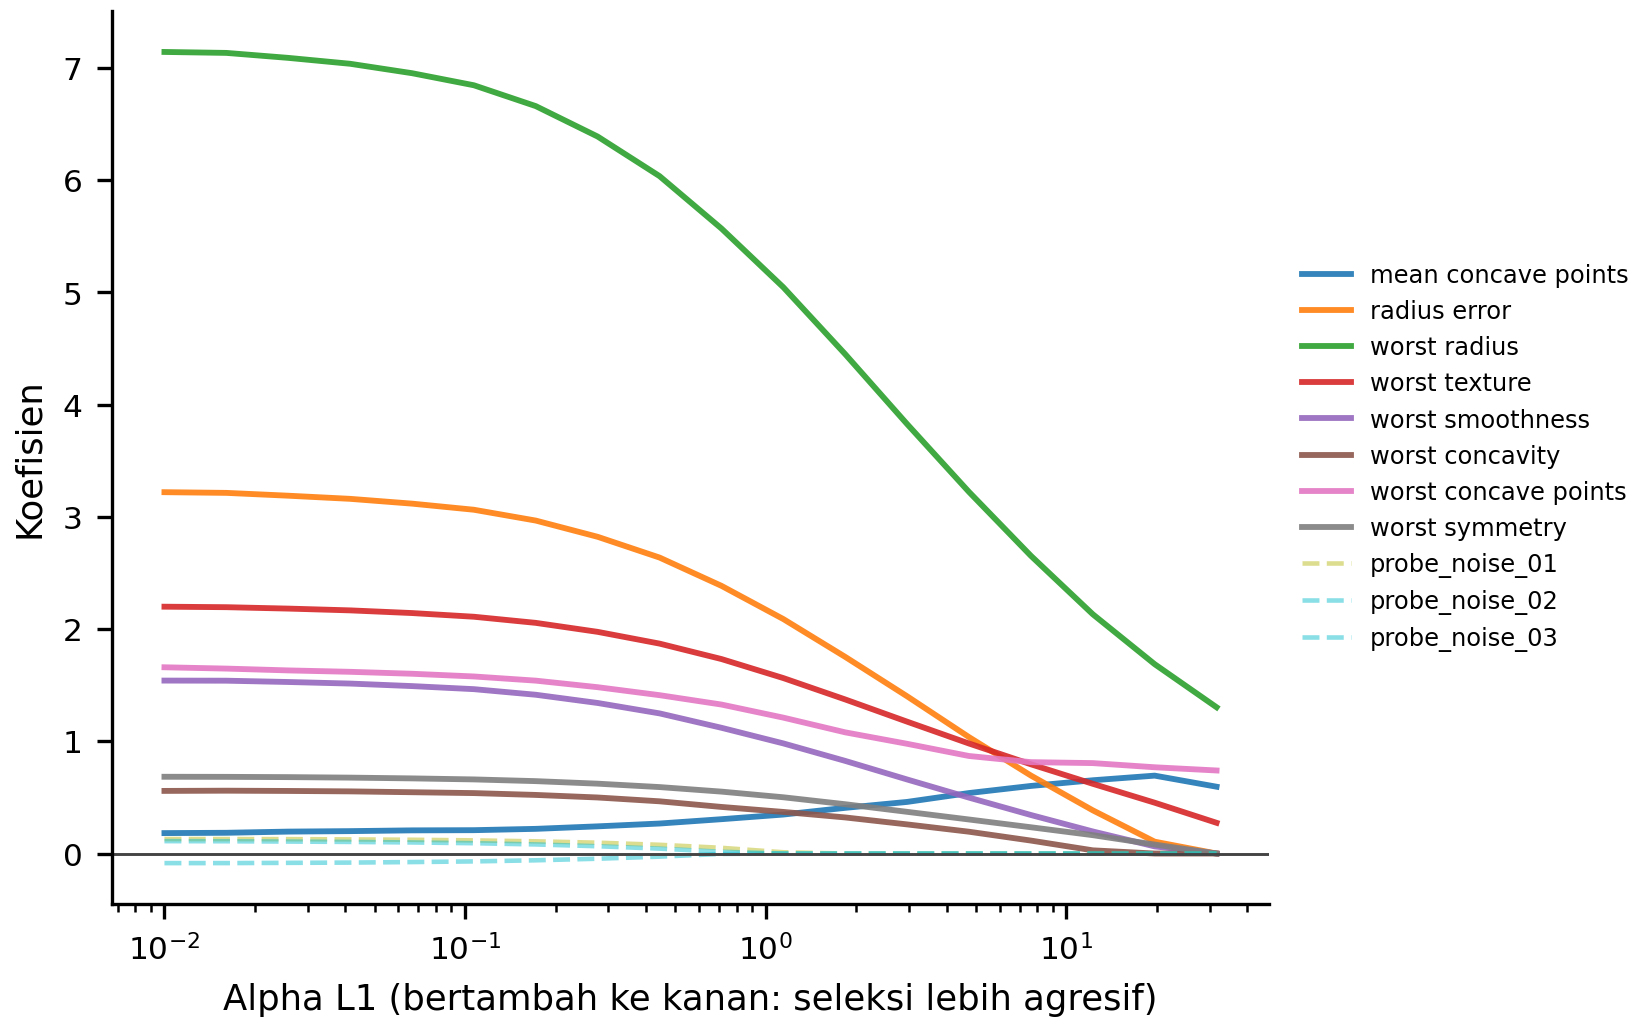
\includegraphics[width=111.6mm]{ch07-fig-3}
\caption{Lintasan penyusutan koefisien pada LASSO}
\label{fig:ch07-fig-3}
\end{figure}

Model pohon dan \emph{ensemble} juga sering memberi \emph{feature importance}. Alur seperti \passthrough{\lstinline!SelectFromModel!} memakai koefisien atau \emph{importance} dari model terlatih untuk memilih fitur. Namun, \emph{importance} tidak netral. Pada model pohon, \emph{importance} dapat bias terhadap fitur berkardinalitas tinggi, fitur dengan banyak titik \emph{split}, atau fitur yang berkorelasi dengan fitur lain. Berbeda dari L1, seleksi berbasis \emph{importance} pohon tidak otomatis menghilangkan redundansi antarfitur dengan cara yang sama. Karena itu, \emph{importance} model sebaiknya diperiksa dengan \emph{permutation importance}, \emph{ablation}, atau evaluasi ulang pada subset yang dipilih.

Tabel 7.1 mengembalikan ketiga keluarga metode ke sumbu perbandingan yang sama. Kolomnya menekankan keputusan praktis tentang kecepatan metode, kemampuan menangkap interaksi, cara menangani redundansi, keterikatan hasil pada model, dan risiko utamanya.

\tabeljudul{Tabel 7.1 — Perbandingan keluarga metode seleksi}

{\def\LTcaptype{none} % do not increment counter
\par\vspace{3pt}\noindent
\begingroup\renewcommand{\arraystretch}{1.0}%
\scriptsize\linespread{1}\selectfont
\renewcommand{\_}{\textunderscore\hspace{0pt}}%
\begin{xltabular}{\linewidth}{@{}>{\raggedright\arraybackslash}p{(\linewidth-10\tabcolsep)*\real{0.126}} >{\raggedright\arraybackslash}p{(\linewidth-10\tabcolsep)*\real{0.160}} >{\raggedright\arraybackslash}p{(\linewidth-10\tabcolsep)*\real{0.158}} >{\raggedright\arraybackslash}p{(\linewidth-10\tabcolsep)*\real{0.160}} >{\raggedright\arraybackslash}p{(\linewidth-10\tabcolsep)*\real{0.111}} >{\raggedright\arraybackslash}p{(\linewidth-10\tabcolsep)*\real{0.285}}@{}}
\toprule

Keluarga
 & 
Kecepatan
 & 
Interaksi
 & 
Redundansi
 & 
Terikat model?
 & 
Risiko utama
 \\
\midrule
\endhead




Filter & Sangat cepat & Tidak & Tidak & Tidak & Meloloskan duplikat dan membuang fitur interaksi \\
Wrapper & Lambat & Tergantung estimator dasar & Dapat & Ya & \emph{Overfitting} prosedur seleksi dan biaya komputasi \\
Embedded & Cepat-sedang & Sebagian, tergantung model & Dapat; L1 bisa tidak stabil pada fitur berkorelasi & Ya & Bias \emph{importance} dan hasil spesifik-model \\
\bottomrule
\end{xltabular}\endgroup\par\vspace{5pt}

}

Metode \emph{embedded} sering menjadi kompromi yang menarik karena lebih dekat ke kecepatan \emph{filter}, tetapi lebih sadar model dan dapat menangani sebagian redundansi. Hasilnya tetap mewarisi bias model yang melakukan seleksi. Jika model pemilih tidak sesuai dengan model akhir atau struktur data, subset yang dihasilkan bisa menyesatkan. Karena itu, Tabel 7.1 perlu dibaca bersama prinsip berikutnya. Seleksi harus dinilai melalui validasi yang tidak ikut dipakai untuk memilih fitur, apa pun keluarga metodenya.

\begin{pendalaman}{Minimal-optimal vs all-relevant sebagai dua filosofi seleksi}
Pendekatan minimal-optimal, seperti LASSO atau mRMR, mencari subset sekecil mungkin yang mempertahankan performa. Ini cocok untuk model produksi yang ringkas. Pendekatan all-relevant berusaha menemukan semua fitur yang membawa sinyal, termasuk fitur yang redundan tetapi bermakna secara ilmiah. Boruta mengikuti filosofi kedua. Metode ini membuat \emph{shadow features} dengan mengacak fitur asli, lalu mempertahankan fitur nyata yang mengalahkan shadow-nya secara statistik. Ide shadow ini berkerabat dengan \emph{probe feature} sebagai pembanding acak, tetapi tujuannya berbeda. Boruta mencari semua sinyal, sementara pembuangan \emph{noise} hanya sebagian dari pekerjaan itu.
\end{pendalaman}

\section{Stabilitas Seleksi dan Validasi Bersarang}\label{stabilitas-seleksi-dan-validasi-bersarang}

Seleksi fitur selalu bergantung pada data (Cawley and Talbot 2010). Jika dilakukan sebelum \emph{train/test split} atau di luar \emph{fold cross-validation}, informasi dari data validasi dapat masuk ke pilihan fitur. Ini bentuk \emph{leakage} yang sering terjadi karena seleksi terasa seperti langkah persiapan biasa. Jika target dipakai untuk memilih fitur, pilihan tersebut sudah dipengaruhi oleh label pada data yang seharusnya menjadi penguji.

Kerusakannya muncul dalam beberapa bentuk. Estimasi performa menjadi terlalu optimistis karena asosiasi target pada data uji ikut terlihat saat seleksi. Objektivitas evaluasi juga hilang karena model secara tidak langsung sudah melihat label uji. Saat produksi, performa dapat runtuh karena fitur yang tampak kuat ternyata hanya cocok dengan kebetulan pada \emph{dataset} penuh.

Jika seleksi fitur dan \emph{tuning} hiperparameter dilakukan bersama, evaluasi sebaiknya memakai \emph{nested validation} atau \emph{test set} yang benar-benar tidak disentuh. \emph{Inner loop} memilih jumlah fitur \(k\), kekuatan L1 \(\alpha\), atau subset terbaik. \emph{Outer loop} menilai performa pada \emph{fold} yang belum dipakai untuk keputusan tersebut. Bab 2 sudah memperkenalkan \emph{nested cross-validation}. Di bagian ini, prinsipnya diterapkan khusus pada seleksi fitur.

Gambar 7.4 membandingkan alur salah dan benar. Pada alur salah, seleksi dilakukan pada seluruh data sebelum \emph{cross-validation}, sehingga informasi dari \emph{fold} validasi masuk ke tahap seleksi. Pada alur benar, setiap \emph{outer fold} memiliki seleksi dan \emph{tuning} di bagian \emph{train}-nya sendiri, lalu dievaluasi pada bagian \emph{outer test} yang belum disentuh.

\begin{figure}[tbp]\centering
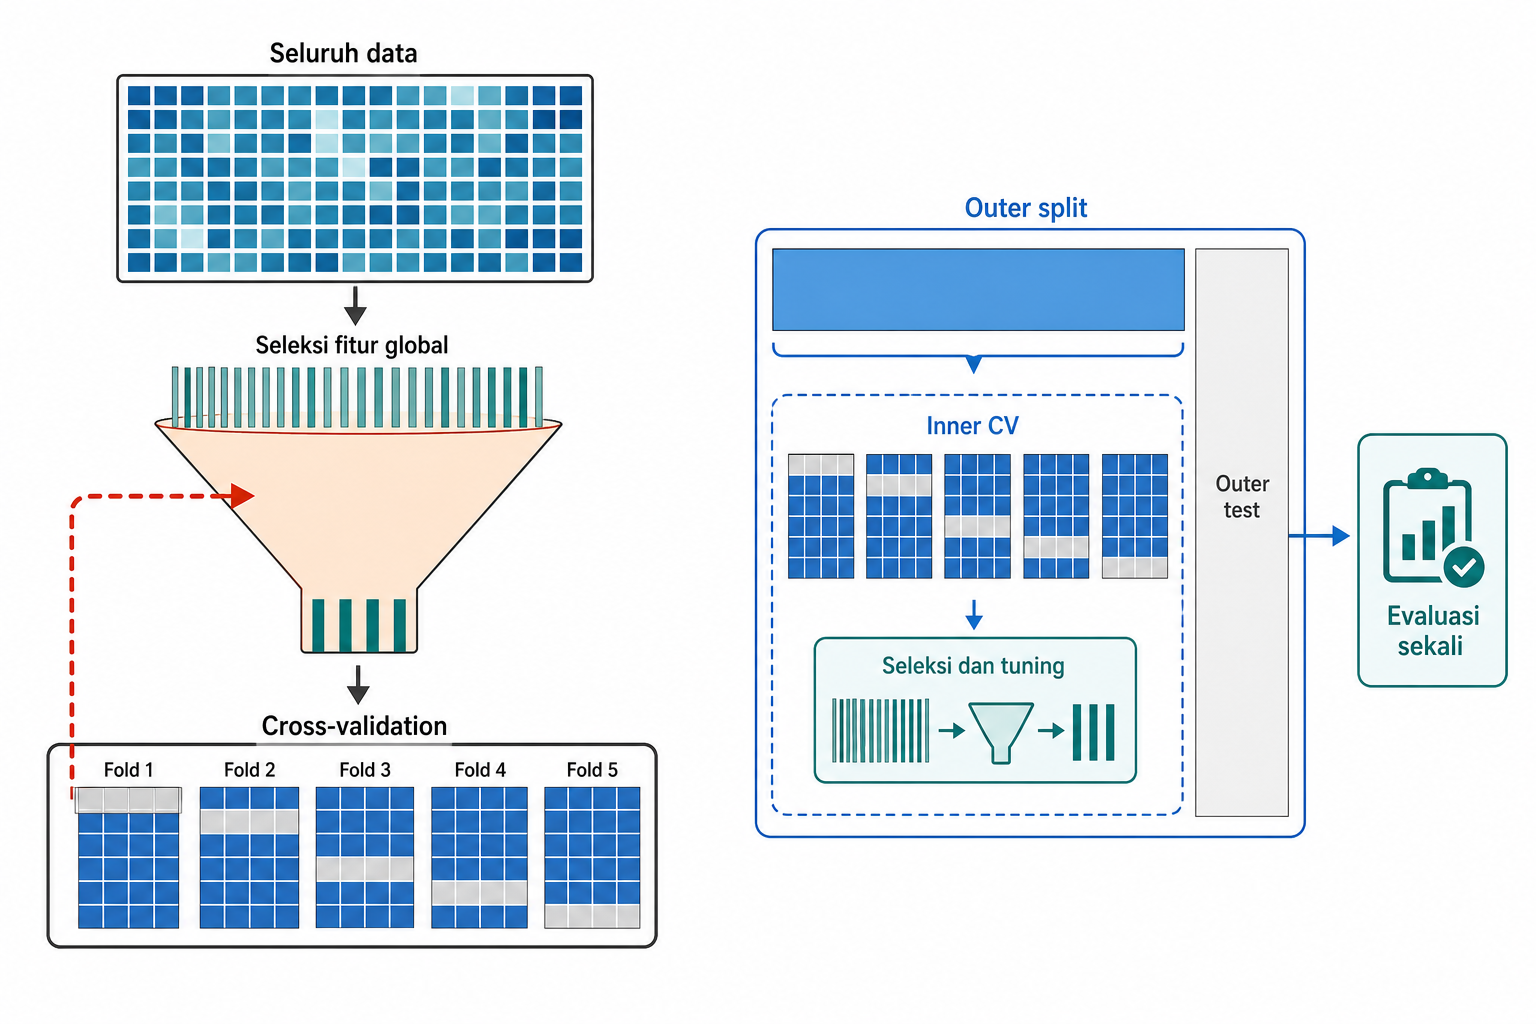
\includegraphics[width=111.6mm]{ch07-fig-4}
\caption{Seleksi fitur salah dan seleksi fitur dalam validasi bersarang}
\label{fig:ch07-fig-4}
\end{figure}

Selain performa, stabilitas juga perlu diperhatikan. Seleksi yang stabil memilih fitur serupa di berbagai \emph{fold}, \emph{resample}, periode waktu, atau populasi. Seleksi yang tidak stabil dapat menandakan sinyal lemah, fitur-fitur pengganti yang saling berkorelasi, sampel terlalu kecil, atau seleksi yang terlalu agresif. Kadang fitur individual berganti-ganti, tetapi kelompok sinyalnya tetap sama. Beberapa ukuran aktivitas pengguna, misalnya, dapat saling menggantikan. Model tidak selalu membutuhkan semuanya, tetapi keluarga fitur aktivitas tetap penting.

Stabilitas tidak berarti fitur harus sama persis di semua situasi. Dunia dapat berubah, populasi dapat bergeser, dan fitur yang relevan pada satu periode mungkin melemah pada periode lain. Namun, jika subset berubah drastis hanya karena \emph{fold} berubah sedikit, hasil seleksi perlu dibaca sebagai tidak pasti.

\begin{pendalaman}{Mengukur stabilitas seleksi}
Stabilitas dapat diukur dengan membandingkan himpunan fitur yang dipilih pada dua fold. Salah satu ukuran sederhana adalah Jaccard index, \(J(A, B) = \dfrac{|A \cap B|}{|A \cup B|}\), dengan \(A\) dan \(B\) sebagai dua himpunan fitur terpilih. Nilai mendekati 1 berarti pilihan sangat mirip, sedangkan nilai mendekati 0 berarti hampir tidak ada irisan. Namun, fitur yang saling berkorelasi dapat menurunkan skor pasangan walaupun kelompok sinyalnya stabil. Pemeriksaan juga perlu mencakup kelompok fitur, bukan hanya nama kolom individual. Stabilitas rendah lebih tepat dibaca sebagai temuan tentang data dan sinyal daripada sebagai kegagalan algoritma semata.
\end{pendalaman}

\begin{sintesis}

Seleksi fitur adalah keputusan representasi untuk menyederhanakan tanpa membuang sinyal penting. Fitur yang baik tidak hanya relevan terhadap target, tetapi juga tidak terlalu mengulang fitur lain, stabil di bawah evaluasi yang sah, dan layak dipelihara dalam sistem. Pada data berdimensi tinggi, seleksi dapat mengurangi \emph{overfitting}, biaya komputasi, dan kesulitan interpretasi, terutama setelah proses pembentukan fitur seperti pada Bab 6.

Metode \emph{filter} cepat dan berguna sebagai penyaringan awal, tetapi mudah melewatkan interaksi dan meloloskan duplikat. Metode \emph{wrapper} lebih dekat dengan model dan metrik tertentu, tetapi mahal dan rentan \emph{overfitting} prosedural. Metode \emph{embedded} melakukan seleksi selama pelatihan, misalnya melalui L1 atau \emph{importance} model, tetapi mewarisi bias model pemilih. Tabel 7.1 merangkum perbedaan ini sebagai peta keputusan, bukan sebagai peringkat mutlak.

Prinsip terpentingnya adalah validasi. Seleksi fitur harus diperlakukan sebagai proses yang belajar dari data, sehingga ditempatkan di dalam \emph{split}, \emph{fold}, atau \emph{nested validation}. Setelah fitur dipilih, hasilnya perlu diperiksa melalui stabilitas subset, ketersediaan saat inferensi, kewajaran secara domain, dan kontribusinya terhadap tujuan model.

\end{sintesis}

\begin{bacaan}

\begin{itemize}
\tightlist
\item
  scikit-learn --- Feature selection --- \url{https://scikit-learn.org/stable/modules/feature_selection.html}. Metode filter, wrapper, dan embedded.
\item
  Beyer dkk. (1999), ``When Is Nearest Neighbor Meaningful?'' --- \url{https://doi.org/10.1007/3-540-49257-7_15}. Konsentrasi jarak di dimensi tinggi.
\item
  Peng dkk. (2005), mRMR (IEEE TPAMI) --- \url{https://doi.org/10.1109/TPAMI.2005.159}. Seleksi minimum-redundancy maximum-relevance.
\item
  Nogueira dkk. (2018), Stability of Feature Selection (JMLR) --- \url{https://jmlr.org/papers/v18/17-514.html}. Mengukur kestabilan hasil seleksi fitur.
\item
  Kursa \& Rudnicki (2010), Boruta (JStatSoft) --- \url{https://doi.org/10.18637/jss.v036.i11}. Wrapper all-relevant berbasis random forest.
\end{itemize}

\end{bacaan}

\rujukanheading

\protect\phantomsection\label{refs}
\begin{CSLReferences}{1}{1}
\bibitem[\citeproctext]{ref-cawley2010overfitting}
Cawley, Gavin C., and Nicola L. C. Talbot. 2010. {``On over-Fitting in Model Selection and Subsequent Selection Bias in Performance Evaluation.''} \emph{Journal of Machine Learning Research} 11: 2079--107.

\bibitem[\citeproctext]{ref-guyon2003selection}
Guyon, Isabelle, and André Elisseeff. 2003. {``An Introduction to Variable and Feature Selection.''} \emph{Journal of Machine Learning Research} 3: 1157--82.

\bibitem[\citeproctext]{ref-tibshirani1996lasso}
Tibshirani, Robert. 1996. {``Regression Shrinkage and Selection via the Lasso.''} \emph{Journal of the Royal Statistical Society, Series B} 58 (1): 267--88.

\end{CSLReferences}

% ==========================================================================
% ch08.tex — dihasilkan otomatis dari website/chapters/ch08.qmd
% Boleh disunting manual. 'sync' hanya menimpa bila .qmd berubah DAN .tex
% belum disunting; kalau keduanya berubah, dilewati (pakai --force).
% qmd-sha1: 469d9a90c33d
% tex-sha1: 1941bd577ac9
% ==========================================================================
% >>>>> ISI OTOMATIS (jangan hapus baris ini) >>>>>
\chapter{Reduksi Dimensi \& Representasi Laten}\label{reduksi-dimensi-representasi-laten}

\section{Mengapa Mereduksi Dimensi? Kompresi vs.~Visualisasi}\label{mengapa-mereduksi-dimensi-kompresi-vs.-visualisasi}

Matriks data berdimensi tinggi sering kali memicu \emph{curse of dimensionality} (kutukan dimensionalitas). Ruang fitur yang terlalu luas dan renggang memperlambat komputasi, membebani memori, serta menaikkan risiko \emph{overfitting} akibat parameter model yang berlebih.

Seleksi fitur mengatasi masalah ini dengan membuang kolom fitur secara diskret. Reduksi dimensi mengambil pendekatan berbeda. Alih-alih membuang atribut, metode ini memadatkan seluruh matriks observasi ke dalam susunan baru yang jauh lebih ringkas. Hasil transformasi ini membentuk ruang berdimensi rendah yang disebut \emph{latent representation} (representasi laten).

Representasi laten menangkap inti struktur sebaran observasi data. Pada ruang baru ini, fitur tereduksi tidak lagi menyimpan makna fisis aslinya. Sumbu fitur awal seperti ``suhu ruang'' tidak lagi berdiri mandiri; atribut baru muncul sebagai paduan matematis yang mendeskripsikan kondisi sistem secara keseluruhan.

Secara matematis, algoritma reduksi mencari fungsi transformasi yang memetakan matriks berdimensi tinggi ke matriks berdimensi rendah:

\[ X_{laten} = f(X) \]

Di mana \(X \in \mathbb{R}^{n \times d}\) adalah matriks fitur asli dengan \(n\) observasi dan \(d\) dimensi mentah, \(f(\cdot)\) adalah fungsi transformasi reduksi, dan \(X_{laten} \in \mathbb{R}^{n \times k}\) adalah representasi laten dengan dimensi baru \(k\), yang memenuhi syarat \(k \ll d\).

Transformasi ke ruang laten diterapkan dalam siklus \emph{machine learning} untuk melayani dua fungsi utama dengan target yang spesifik:

\begin{itemize}
\tightlist
\item
  \textbf{Kompresi (Prapemrosesan Model):} Transformasi dirancang untuk menekan \emph{noise} dan membuang redundansi antarfitur, sambil tetap mengamankan struktur informasi utama. Contohnya, algoritma memampatkan 100 fitur sensor mentah menjadi 10 dimensi laten yang solid. Matriks 10 dimensi inilah yang diteruskan ke model pengklasifikasi. Kompresi membantu model mempelajari struktur data asli secara efisien tanpa terdistorsi observasi semu.
\item
  \textbf{Visualisasi Analitis:} Ditujukan murni bagi persepsi penglihatan manusia. Matriks ditarik dan ditekan ke kanvas spasial dua atau tiga dimensi agar sebaran pola data dapat diinspeksi. Plot ruang laten membantu analis melihat formasi klaster alami atau mempermudah lokalisasi data pencilan (\emph{outlier}).
\end{itemize}

\begin{figure}[htbp]\centering
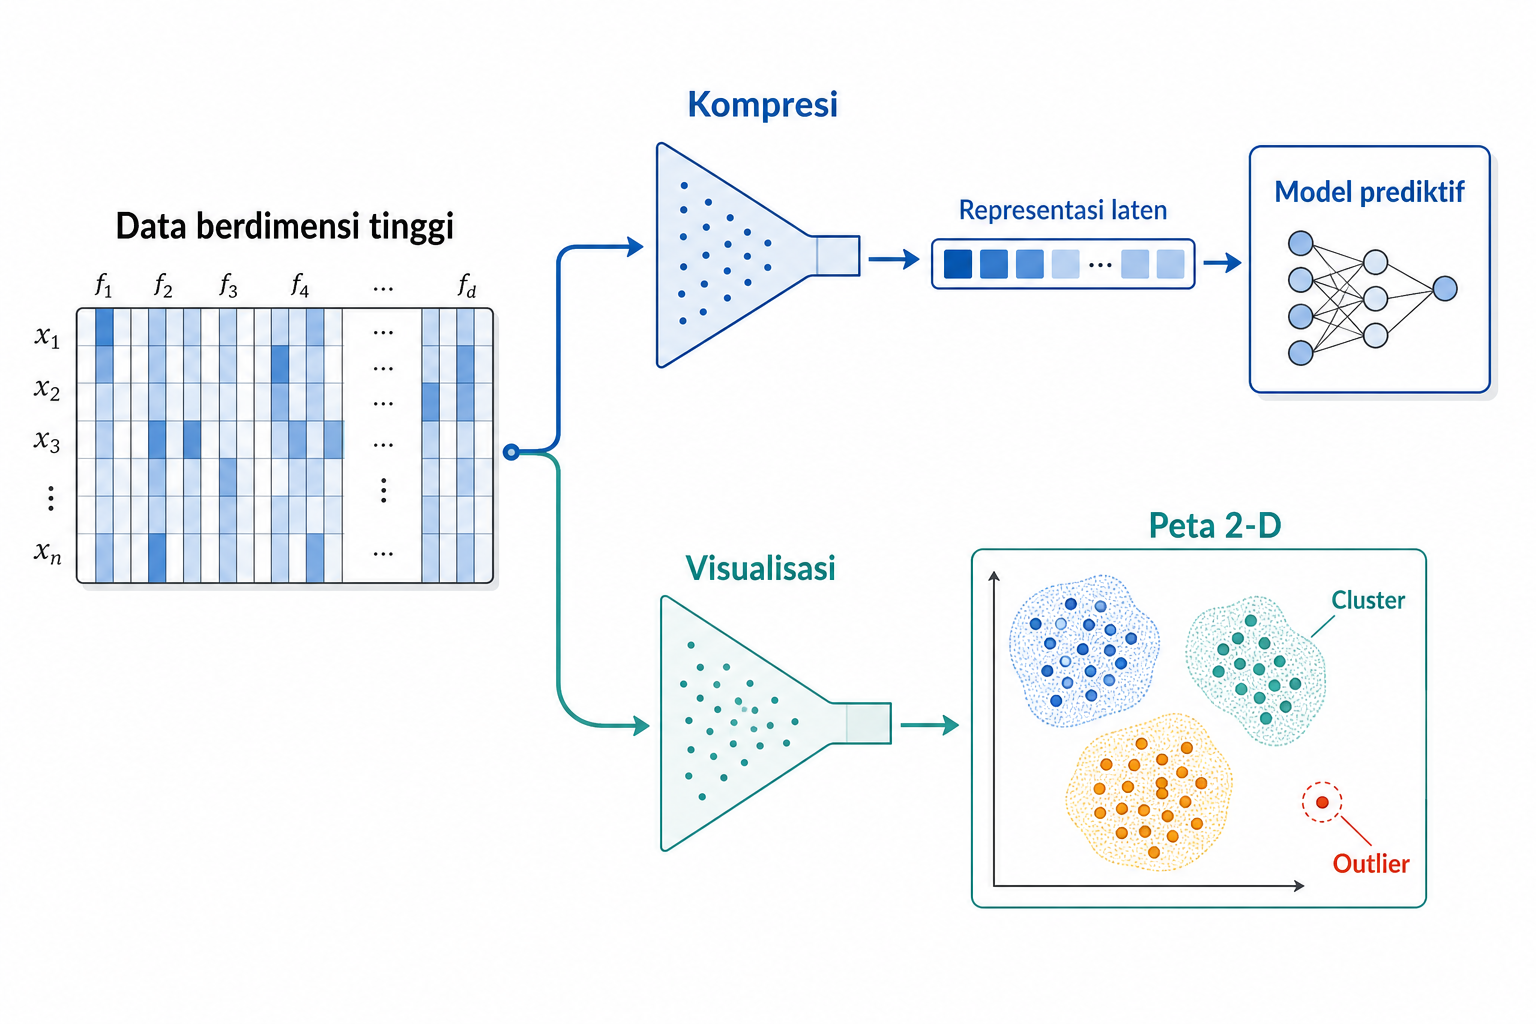
\includegraphics[width=\linewidth,height=0.72\textheight,keepaspectratio]{ch08-fig-1}
\caption{Visualisasi Ruang Fitur dari Dimensi Tinggi (3D) ke Laten 2D}
\label{fig:ch08-fig-1}
\end{figure}

Kedua fungsi ini tidak dapat saling dipertukarkan. Menggunakan matriks visualisasi 2D sebagai prapemrosesan langsung untuk melatih model klasifikasi akan menurunkan kinerja prediksi secara tajam, karena bingkai 2D memotong terlalu banyak detail keragaman data. Sebaliknya, kompresi 10 dimensi sangat ideal untuk komputasi model, tetapi mustahil diinspeksi secara geometris oleh mata. Pemilihan algoritma transformasi bergantung langsung pada tujuan akhir fungsinya.

Eksplorasi reduksi dimensi modern tersebar ke dalam beberapa taksonomi metode:

\begin{itemize}
\tightlist
\item
  \textbf{Linier:} Transformasi lurus berbasis matriks seperti PCA, SVD, dan NMF.
\item
  \textbf{Non-linier:} Pemetaan yang menjaga jarak kelokalan pada \emph{manifold learning} (seperti t-SNE dan UMAP) serta kompresi \emph{neural network} pada \emph{autoencoder}.
\item
  \textbf{Hybrid:} Rangkaian gabungan berurut, misalnya menekan dimensi padat menggunakan PCA sebelum memetakannya ke UMAP untuk stabilisasi \emph{clustering} visual.
\end{itemize}

Implementasi taksonomi metode reduksi di atas membawa konsekuensi operasional lanjutan. Tantangan terbesarnya adalah memilih target kuantitatif dimensi laten (\(k\)). Pendekatan usang menggunakan ukuran proporsi varians yang disederhanakan (misalnya memotong di 95\% varians). Praktik modern menuntut landasan teknis yang lebih kuat, baik dengan pendekatan penaksiran dimensi intrinsik (\emph{intrinsic-dimensionality estimation}), pengujian komparatif \emph{parallel analysis} terhadap matriks acak, atau optimasi murni melalui skema \emph{cross-validation} yang terikat selaras pada skor performa model akhir.

Tantangan kedua berada pada area privasi. Kompresi matriks melalui metode linier seperti PCA maupun dekomposisi berlapis pada \emph{autoencoder} merupakan operasi transformasi \emph{reversible} (sebagian data dapat dikonstruksi ulang ke ruang asalnya). Matriks fitur yang diklaim terkompresi secara anonim masih menahan struktur geometri asli observasi. Sisa struktur ini berpotensi membocorkan identitas tersembunyi atau menyebarkan \emph{bias} dari atribut \emph{proxy} yang dilindungi. Konsekuensi keamanan privasi pada teknik fitur ini akan diurai lebih lanjut pada Bab 9.

\section{PCA dan Keluarga Reduksi Linier}\label{pca-dan-keluarga-reduksi-linier}

\emph{Principal Component Analysis} (PCA) adalah metode reduksi dimensi linier yang paling luas penggunaannya. Pendekatan ini bekerja dengan mencari sumbu-sumbu koordinat baru yang dinamakan komponen utama. Komponen pertama diposisikan pada arah yang menangkap varians terbesar dari kumpulan data, dan komponen-komponen selanjutnya ditarik tegak lurus (ortogonal) terhadap satu sama lain, menangkap sisa varians secara berurutan.

Sebagian besar implementasi modern menghitung PCA tidak melalui dekomposisi matriks kovarians, melainkan menggunakan algoritma \emph{Singular Value Decomposition} (SVD) yang lebih stabil secara numerik. SVD memfaktorkan matriks data masukan \(X \in \mathbb{R}^{n \times d}\) menjadi tiga elemen penyusun:

\[ X = U \Sigma V^T \]

Di mana:

\begin{itemize}
\tightlist
\item
  \(X\) mewakili matriks data yang telah dipusatkan (setiap kolom dikurangi dengan nilai rata-ratanya).
\item
  \(U\) adalah matriks ortogonal yang berisi kumpulan vektor singular kiri.
\item
  \(\Sigma\) adalah matriks diagonal yang menyimpan nilai-nilai singular sebagai representasi besaran varians tiap sumbu.
\item
  \(V^T\) adalah \emph{transpose} dari matriks vektor singular kanan, yang bertindak sebagai komponen utama matriks tersebut.
\end{itemize}

Untuk mereduksi dimensi data dari \(d\) menjadi dimensi target \(k\), proyeksi fitur yang baru dihasilkan dengan memotong matriks transformasi tersebut:

\[ X_{reduced} = X W_k \]

Dalam persamaan ini, \(W_k\) merupakan matriks dimensi \(d \times k\) yang hanya mengambil \(k\) vektor kolom pertama dari matriks komponen utama \(V\).

\begin{figure}[htbp]\centering
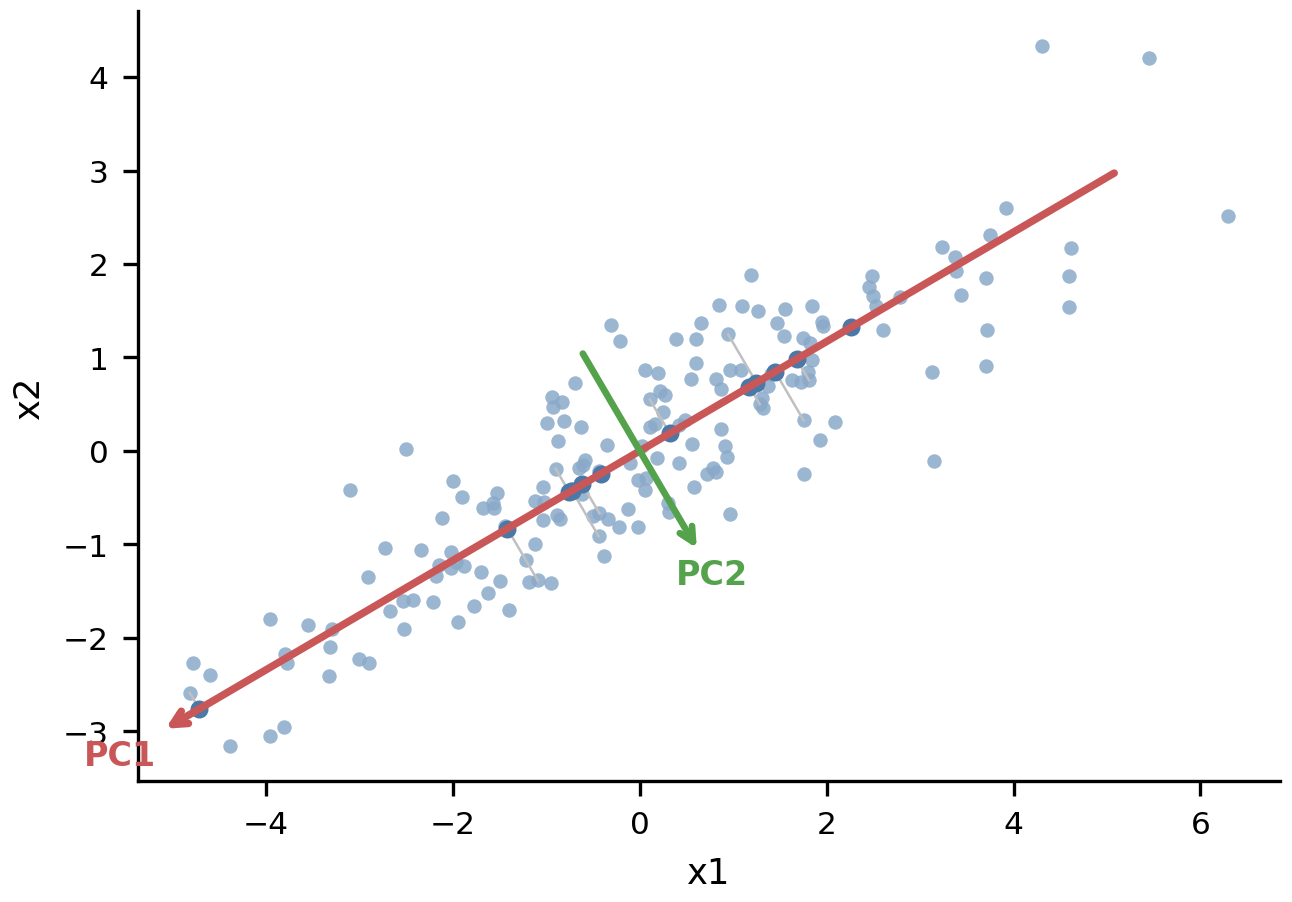
\includegraphics[width=\linewidth,height=0.72\textheight,keepaspectratio]{ch08-fig-2}
\caption{Diagram Vektor Eigen dan Proyeksi Komponen Utama untuk Varians Terbesar}
\label{fig:ch08-fig-2}
\end{figure}

\textbf{Ekstensi dan Varian PCA.}\label{ekstensi-dan-varian-pca}

Dalam praktik pengembangan \emph{machine learning}, satu versi PCA standar sering kali tidak mencukupi untuk berbagai konstrain komputasi. Implementasi pustaka modern menyediakan variasi dekomposisi linier:

\begin{itemize}
\tightlist
\item
  \textbf{Penskalaan Wajib:} PCA memusatkan fitur ke titik nol, namun tidak mengubah skalanya. Skala asli yang besar akan mendominasi perhitungan varians. Penskalaan (misalnya menggunakan fungsi \passthrough{\lstinline!StandardScaler!}) wajib dilakukan sebelum transformasi PCA beroperasi.
\item
  \textbf{Truncated SVD:} Mengurangkan rata-rata pada matriks yang sangat \emph{sparse} (seperti vektor teks TF-IDF) akan mengubah nilai-nilai nol menjadi non-nol, sehingga langsung menghancurkan struktur efisiensi matriks dan berisiko memenuhi kapasitas memori. \emph{Truncated SVD} menyelesaikan faktorisasi tanpa proses pemusatan rata-rata sebelumnya, menjadikannya pilihan teknis untuk data tekstual.
\item
  \textbf{Incremental PCA:} Ketika volume data terlampau besar untuk ditampung memori sistem secara penuh (\emph{out-of-core}), metode ini memperbarui proses dekomposisi secara bertahap menggunakan potongan-potongan \emph{mini-batch}.
\item
  \textbf{Randomized SVD:} Saat jumlah target komponen \(k\) jauh lebih kecil ketimbang dimensi fitur asli \(d\), pendekatan stokastik ini memotong waktu komputasi secara drastis sambil memberikan aproksimasi vektor komponen utama yang akurat.
\end{itemize}

\textbf{Whitening dan Kompresi Embedding Terlatih.}\label{whitening-dan-kompresi-embedding-terlatih}

Fungsi reduksi dimensi sering menyediakan parameter untuk melakukan penskalaan ulang ruang fitur yang disebut proses \emph{whitening}. Operasi ini memaksa komponen-komponen utama yang dihasilkan memiliki varians satuan yang seragam (isotropik). \emph{Whitening} memfasilitasi perbandingan kemiripan fitur dalam metode pencarian jarak dekat (\emph{retrieval}), namun pemaksaan ini membuang pola variasi anisotropik yang sering kali dibutuhkan oleh model klasifikasi untuk menentukan pemisahan garis batas label.

Meskipun algoritma non-linier memiliki visualisasi yang lebih padat, metode linier tetap relevan dalam kompresi \emph{embedding} pra-latih (seperti representasi Transformer yang akan dibahas pada Bab 15). PCA linier mampu mereduksi hingga 50\% dimensi awal \emph{sentence embedding} tanpa degradasi metrik sistem kompresi secara bermakna. Proses PCA menahan distorsi performa representasi fitur jauh lebih baik ketimbang kompresi menggunakan \emph{autoencoder} maupun proyeksi UMAP.

\section{Representasi Berbasis Bagian: Non-negative Matrix Factorization (NMF)}\label{representasi-berbasis-bagian-non-negative-matrix-factorization-nmf}

Pendekatan dekomposisi linier seperti PCA sering menghasilkan komponen laten yang mengandung percampuran nilai positif dan negatif. Representasi padat semacam ini menyulitkan proses interpretasi. Secara alamiah, manusia kesulitan menafsirkan fitur gabungan yang dibangun melalui proses pengurangan matematis. Sebagai contoh, mustahil membayangkan rekonstruksi citra wajah dengan cara merangkai komponen bentuk dasar lalu ``mengurangi'' bagian mata secara aljabar.

Jika interpretabilitas merupakan tuntutan utama dan observasi data orisinil memuat nilai tak-negatif, pendekatan \emph{Non-negative Matrix Factorization} (NMF) menawarkan model ekstraksi yang jauh lebih natural. Algoritma ini memberlakukan batasan ketat: matriks input maupun kedua matriks luarannya sama sekali tidak diizinkan memiliki angka di bawah nol.

Ketentuan aljabar tersebut memaksa algoritma merangkai ruang dimensi baru secara murni melalui operasi penambahan. Sifat seratus persen aditif ini melahirkan \emph{parts-based representation} (representasi berbasis bagian). Setiap fitur laten bertindak layaknya kepingan blok independen yang saling melengkapi untuk membangun wujud data utuh.

Proses dekomposisi NMF didefinisikan secara formal melalui hampiran perkalian matriks:

\[ X \approx W H \]

Pada formulasi tersebut:

\begin{itemize}
\tightlist
\item
  \(X \in \mathbb{R}_{+}^{n \times d}\) adalah matriks observasi tak-negatif yang terdiri dari \(n\) sampel dan \(d\) fitur.
\item
  \(W \in \mathbb{R}_{+}^{n \times k}\) mewakili matriks aktivasi, menampung bobot koefisien yang mengendalikan seberapa besar porsi setiap komponen digunakan untuk membangun ulang tiap sampel observasi.
\item
  \(H \in \mathbb{R}_{+}^{k \times d}\) bertindak sebagai matriks komponen laten (\(k\)), menyimpan kamus pola dasar yang merepresentasikan elemen penyusun data.
\end{itemize}

\begin{figure}[htbp]\centering
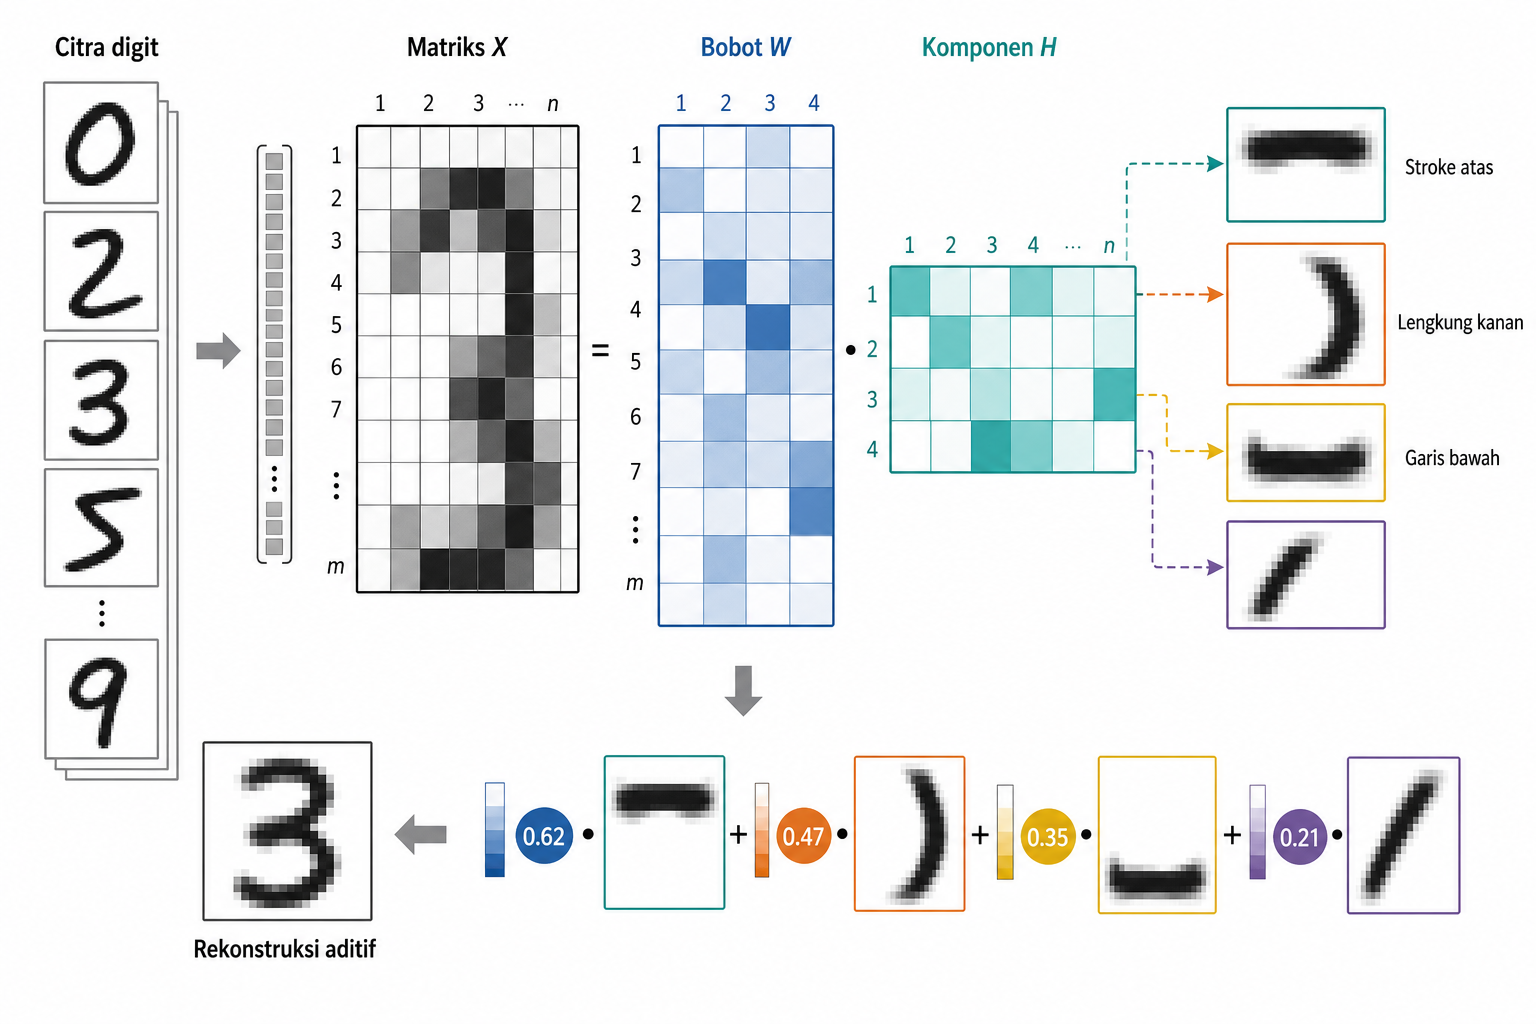
\includegraphics[width=\linewidth,height=0.72\textheight,keepaspectratio]{ch08-fig-3}
\caption{Dekomposisi Matriks NMF: X = W * H}
\label{fig:ch08-fig-3}
\end{figure}

\textbf{Fungsi Kerugian \(\beta\)-divergence.}\label{fungsi-kerugian-beta-divergence}

NMF tidak bekerja dengan memutar sumbu orthogonal seperti PCA, melainkan mencari hampiran terdekat dari \(X\) menggunakan optimasi fungsi kerugian matematis. Dalam perwujudan modernnya, kualitas rekonstruksi dievaluasi melalui keluarga jarak pengukuran yang disebut \(\beta\)-divergence (divergensi \(\beta\)).

Nilai \(\beta\) memengaruhi bentuk kompresi dan perlu disesuaikan dengan distribusi tipe data masukan:

\begin{itemize}
\tightlist
\item
  \textbf{\(\beta=2\) (Frobenius norm):} Fungsi standar yang paling umum dipakai dan efektif pada sebaran data numerik berkelanjutan yang tak-negatif.
\item
  \textbf{\(\beta=1\) (Kullback-Leibler divergence):} Sangat cocok untuk representasi frekuensi cacahan atau data teks.
\item
  \textbf{\(\beta=0\) (Itakura-Saito divergence):} Pilihan yang didesain secara spesifik untuk menangkap rentang dinamis besar, menjadikannya standar pada spektrum daya audio.
\end{itemize}

\textbf{Aspek Komputasi dan Skalabilitas.}\label{aspek-komputasi-dan-skalabilitas}

Sebagai representasi yang murni dioptimasi, penerapan NMF memerlukan perhatian pada beberapa aspek teknis implementasi:

\begin{itemize}
\tightlist
\item
  \textbf{Sensitivitas inisialisasi:} Fungsi kerugian NMF tidak memiliki titik minimum global tunggal. Inisialisasi secara acak membuat performanya tidak stabil. Pendekatan inisialisasi matematis deterministik, seperti NNDSVD (\emph{Nonnegative Double Singular Value Decomposition}), mempercepat konvergensi secara signifikan pada data berdimensi jarang (\emph{sparse}).
\item
  \textbf{Efisiensi pemrosesan:} Algoritma NMF konvensional membutuhkan ketersediaan seluruh data di memori. Untuk himpunan data bervolume raksasa, metode seperti \emph{MiniBatchNMF} mengadopsi partisi data kecil, mengizinkan pembaharuan model tanpa memuat keseluruhan matriks secara serentak.
\item
  \textbf{Kontrol sparsitas:} Melalui injeksi nilai penalti (L1 maupun L2) terhadap matriks \(W\) atau \(H\), struktur representasi laten dapat dipaksa untuk lebih renggang (\emph{sparse}), membatasi agar satu dokumen atau sinyal dibangun dari sesedikit mungkin fitur penyusun dasar.
\end{itemize}

\textbf{Domain Aplikasi Spesifik.}\label{domain-aplikasi-spesifik}

Karakter aditif dari NMF menjadi sangat aplikatif pada domain data yang secara alamiah terbentuk lewat konsep superposisi fisis maupun logis:

\begin{itemize}
\tightlist
\item
  \textbf{Pemodelan teks dan dokumen:} Sebuah tulisan logisnya merupakan gabungan proporsional dari beberapa topik, bukan ``pengurangan'' antar topik. Melalui perpaduan fungsi \(\beta=1\), NMF memfasilitasi algoritma mengelompokkan kosakata yang sering muncul bersama menjadi klaster fitur topik yang langsung bisa dibaca dan ditafsirkan manusia.
\item
  \textbf{Dekomposisi sinyal audio:} Perpaduan harmonis berbagai instrumen pada satu rekaman muncul melalui penjumlahan getaran frekuensi. Sebuah instrumen perkusi murni menyuntikkan energi getaran ke udara. Penggunaan NMF dengan divergensi \(\beta=0\) meniru perilaku superposisi dunia nyata ini dengan akurasi tinggi, menjadikannya ekstraktor fitur standar sebagai pendamping representasi \emph{spectrogram}.
\end{itemize}

\section{Manifold Learning: t-SNE dan UMAP}\label{manifold-learning-t-sne-dan-umap}

Metode reduksi linier seperti PCA merangkum variansi dengan membuat proyeksi sumbu ortogonal. Pendekatan ini gagal memisahkan data yang memiliki geometri lipatan non-linier, seperti pada bentuk \emph{Swiss roll}. Pada struktur tersebut, jarak lurus (Euclidean) antar-titik menembus ruang kosong antar-lipatan sehingga tidak merepresentasikan kedekatan spasial yang sebenarnya. Jarak relasional ini hanya dapat dihitung dengan mengikuti kelengkungan permukaan data yang disebut sebagai \emph{manifold}.

Algoritma \emph{manifold learning} memodelkan data dengan asumsi bahwa titik-titik tersebut terletak pada sebuah \emph{manifold} berdimensi rendah yang terlipat di dalam ruang berdimensi tinggi. Untuk keperluan analisis dan reduksi visual, t-SNE dan UMAP menjadi dua metode yang mendominasi.

\textbf{t-SNE (\emph{t-Distributed Stochastic Neighbor Embedding}).}\label{t-sne-t-distributed-stochastic-neighbor-embedding}

Algoritma t-SNE meminimalkan perbedaan probabilitas kedekatan antar-titik di dimensi asal dengan representasinya di dimensi rendah. Fungsi objektif yang dioptimasi menggunakan formulasi \emph{Kullback-Leibler (KL) divergence}:

\[ KL(P || Q) = \sum_{i} \sum_{j \neq i} p_{ij} \log \frac{p_{ij}}{q_{ij}} \]

Di mana \(p_{ij}\) merupakan probabilitas ketetanggaan pasangan data di dimensi tinggi yang diukur menggunakan distribusi Gaussian, sedangkan \(q_{ij}\) mewakili probabilitas pada dimensi sasaran menggunakan distribusi \emph{Student-t} untuk mencegah penumpukan titik data (\emph{crowding problem}).

Metode t-SNE secara ekstrem memaksa kelompok data yang bertetangga agar terus berdampingan di koordinat visual. Karakteristik ini menghasilkan separasi klaster lokal yang baik, namun membawa tiga kelemahan praktis:

\begin{itemize}
\tightlist
\item
  Waktu komputasi sangat lambat akibat pencarian ketetanggaan pada dataset berskala besar.
\item
  Jarak visual antar-klaster tidak merepresentasikan hubungan topologi global. Kelompok data yang berjauhan diposisikan secara sembarang.
\item
  Luas area sebuah klaster pada plot tidak memiliki makna kepadatan, karena algoritma t-SNE memberlakukan pemerataan densitas (\emph{density-equalizing}) terhadap semua populasi klaster.
\end{itemize}

\textbf{UMAP (\emph{Uniform Manifold Approximation and Projection}).}\label{umap-uniform-manifold-approximation-and-projection}

Untuk menutupi kelambatan t-SNE, standar terapan kini beralih pada UMAP. Algoritma ini berlandaskan pada geometri Riemannian dan topologi aljabar untuk membuat perkiraan jaringan dari titik-titik sampel.

\begin{figure}[htbp]\centering
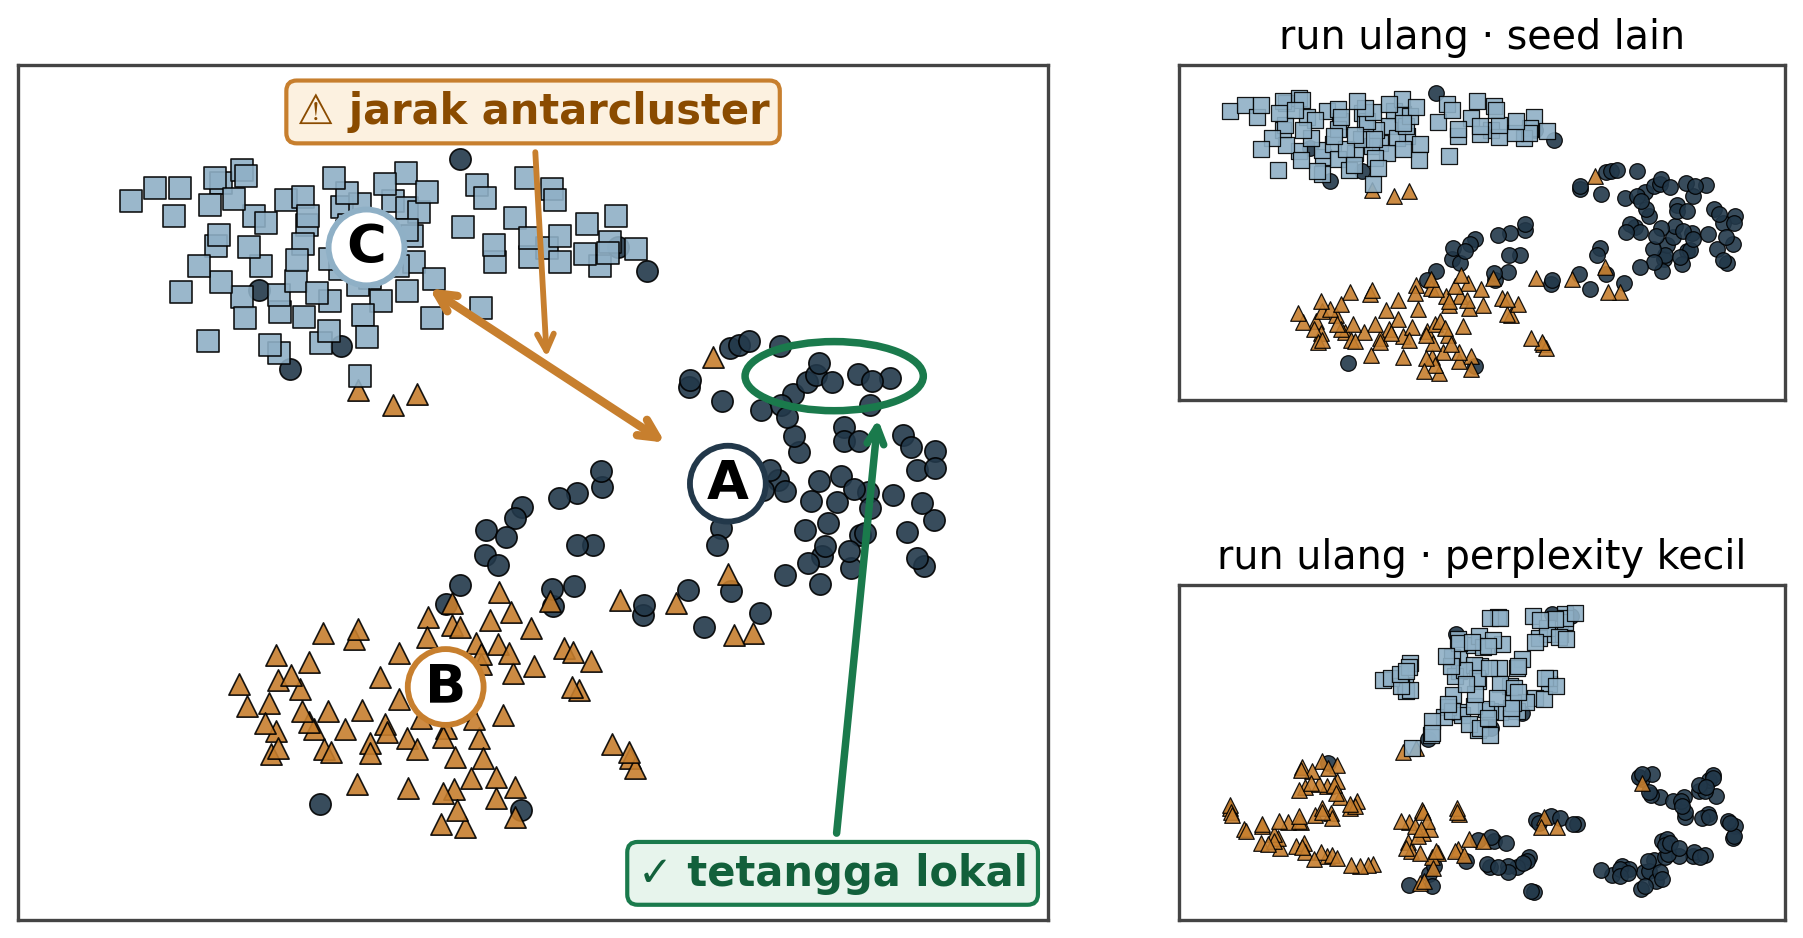
\includegraphics[width=\linewidth,height=0.72\textheight,keepaspectratio]{ch08-fig-4}
\caption{Simplicial Complex pada UMAP untuk Membangun Topologi}
\label{fig:ch08-fig-4}
\end{figure}

Keunggulan utama UMAP adalah kecepatan eksekusinya, serta kemampuannya untuk mereduksi ke dimensi yang lebih leluasa dari sekadar format 2D atau 3D. Literatur awal sering menyebut UMAP lebih superior dalam menjaga penataan struktur global dibandingkan t-SNE. Literatur riset terbaru mengoreksi klaim tersebut; UMAP mempertahankan struktur global karena secara bawaan algoritma ini menggunakan inisialisasi awal berbasis PCA. Apabila t-SNE dan UMAP diatur dengan parameter inisialisasi (PCA) yang sama, kemampuan keduanya dalam mempertahankan struktur relasi berskala global berada pada tingkat yang sebanding.

\textbf{Perkembangan Varian Manifold (2019--2026).}\label{perkembangan-varian-manifold-20192026}

Penelitian algoritma \emph{manifold} terus mengejar keseimbangan antara pelestarian lokal dan global, serta mengakomodasi kekurangan algoritma transaksional t-SNE dan UMAP:

\begin{itemize}
\tightlist
\item
  \textbf{PaCMAP:} Mengontrol keseimbangan skala tata letak data dengan mengategorikan titik menjadi \emph{near}, \emph{mid-near}, dan \emph{further pairs} selama fase kalkulasi.
\item
  \textbf{TriMap:} Menggunakan kalkulasi berbasis orientasi kelompok (\emph{triplets}) untuk menggantikan pengukuran rasio berpasangan biasa, sehingga susunan jarak global dan hierarki klaster terbangun lebih konsisten.
\item
  \textbf{densMAP:} Modifikasi UMAP yang mengintegrasikan ukuran variansi lokal, sehingga jarak tampilan pada plot berhasil mencerminkan volume densitas titik yang sebenarnya.
\item
  \textbf{DREAMS dan PCC:} Pendekatan modern tahun 2025--2026 yang secara paralel memfasilitasi optimalisasi jarak korelasi metrik dengan pemisahan margin layaknya t-SNE.
\end{itemize}

Meskipun tangguh untuk membuat segmentasi, fungsionalitas murni metode ini berpusat pada penelusuran gambaran visual kelompok klaster, bukan teknik \emph{preprocessing} data yang ideal bagi \emph{machine learning}. Algoritma \emph{manifold} awal ini sepenuhnya transduktif; mereka memerlukan populasi matriks penuh guna membentangkan topologi, sehingga sulit diintegrasikan pada lingkungan arsitektur \emph{inference} otomatis untuk mentransformasikan fitur pada baris data tunggal.

\section{Autoencoder sebagai Kompresi yang Dipelajari}\label{autoencoder-sebagai-kompresi-yang-dipelajari}

Metode linier seperti PCA mencari sumbu varians maksimal, sementara algoritma manifold berfokus pada geometri lokal titik data. \emph{Autoencoder} mengambil jalur yang berbeda: melatih \emph{neural network} agar memadatkan data ke dalam ruang laten berdimensi rendah, lalu berusaha merekonstruksinya kembali. Pendekatan ini memetakan matriks masukan melalui representasi yang dipelajari mesin, dengan satu batasan tegas: model murni menekan data internal yang dimilikinya, bukan mentransfer semantik atau pemahaman dari luar.

\begin{figure}[htbp]\centering
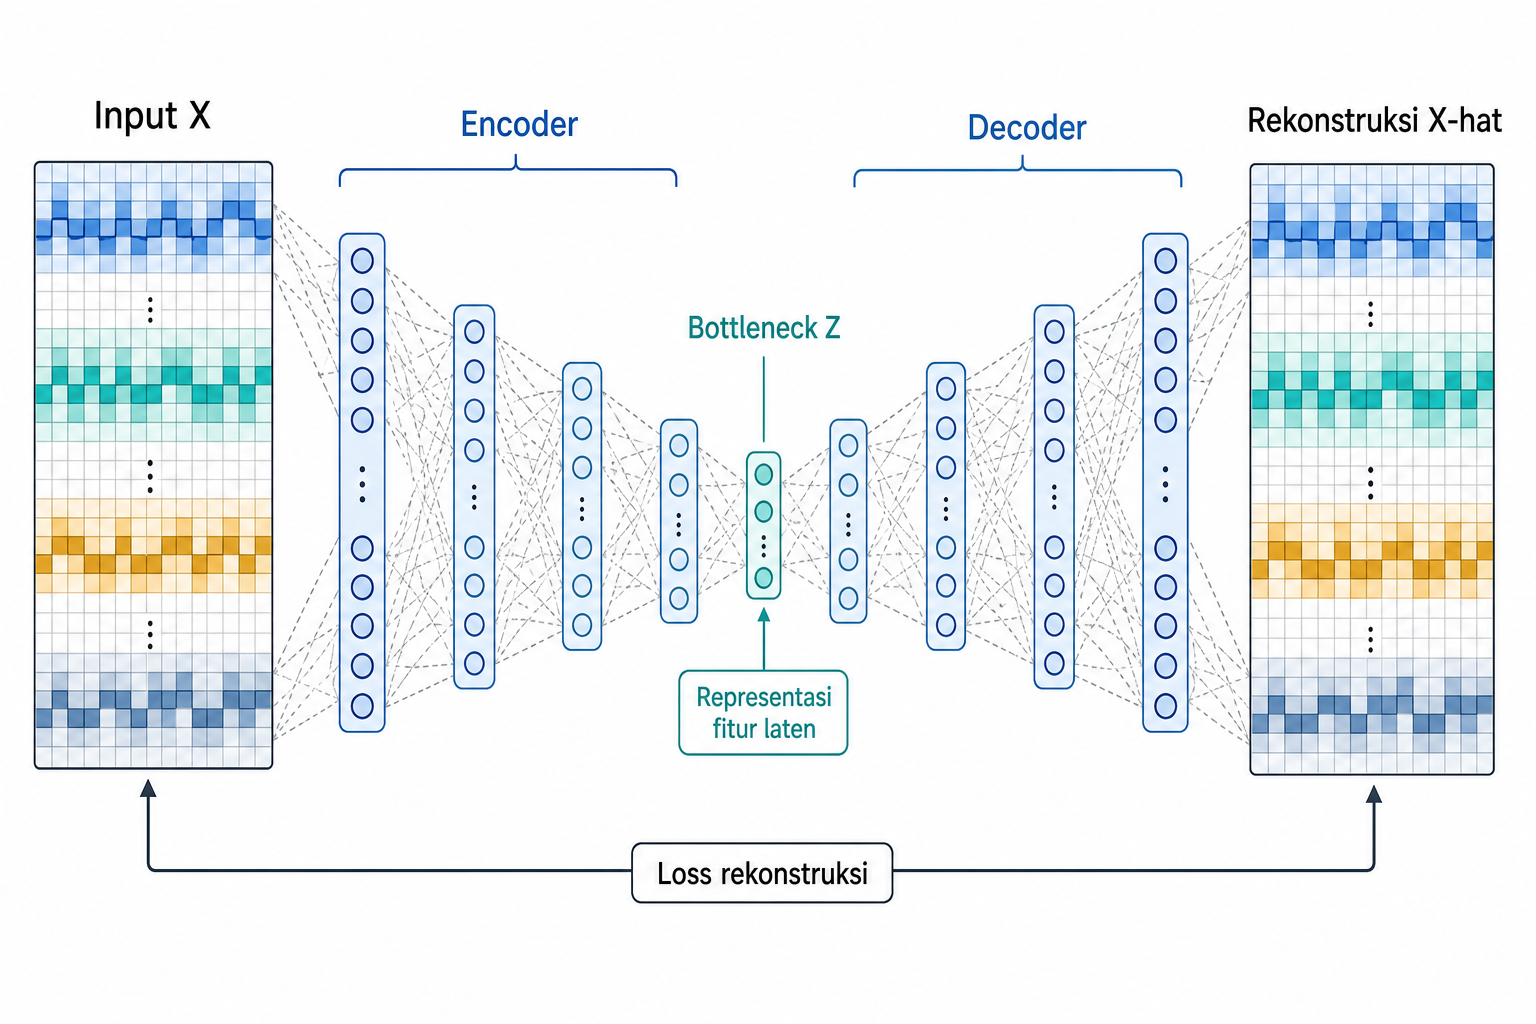
\includegraphics[width=\linewidth,height=0.72\textheight,keepaspectratio]{ch08-fig-5}
\caption{Skema Arsitektur Autoencoder: Encoder, Bottleneck, Decoder}
\label{fig:ch08-fig-5}
\end{figure}

\textbf{Arsitektur Dasar: Encoder dan Decoder.}\label{arsitektur-dasar-encoder-dan-decoder}

\emph{Autoencoder} standar terdiri dari dua komponen jaringan saraf yang dioptimalkan secara bersamaan:

\begin{itemize}
\tightlist
\item
  \textbf{Encoder:} Fungsi parametrik \(f_{\theta}\) yang memadatkan matriks fitur masukan \(X\) menjadi representasi laten \(Z\) berdimensi lebih rendah.
\item
  \textbf{Decoder:} Fungsi parametrik \(g_{\phi}\) yang memetakan ruang laten \(Z\) menjadi tebakan matriks asli, dilambangkan dengan \(\hat{X}\).
\end{itemize}

Kapasitas dimensi di lapisan tengah (\emph{bottleneck}) sengaja didesain sangat sempit. Pembatasan ini mencegah jaringan sekadar menyalin masukan ke keluaran. Model terpaksa mengabaikan \emph{noise} dan hanya mempertahankan komponen struktural paling padat untuk membentuk vektor laten.

Pembaruan bobot jaringan dilakukan dengan meminimalkan \emph{reconstruction loss}, yaitu selisih jarak antara data asli dan hasil rekonstruksi:

\[ \mathcal{L}(X, \hat{X}) = \|X - g_{\phi}(f_{\theta}(X))\|^2 \]

Di mana:

\begin{itemize}
\tightlist
\item
  \(X\) adalah vektor fitur masukan.
\item
  \(\hat{X}\) adalah vektor hasil rekonstruksi oleh \emph{decoder}.
\item
  \(f_{\theta}\) dan \(g_{\phi}\) adalah fungsi \emph{neural network} dengan bobot \(\theta\) dan \(\phi\).
\item
  \(\| \cdot \|^2\) melambangkan \emph{Mean Squared Error} (MSE) sebagai jarak kesalahan.
\end{itemize}

\textbf{Varian Autoencoder untuk Fitur Laten.}\label{varian-autoencoder-untuk-fitur-laten}

Jaringan \emph{autoencoder} murni berisiko hanya menghafal posisi data pelatihan tanpa memahami strukturnya jika kapasitasnya berlebih. Agar ruang laten menghasilkan representasi fitur yang kokoh untuk pemodelan tahap selanjutnya, arsitektur ini memiliki beberapa modifikasi:

\begin{itemize}
\tightlist
\item
  \textbf{Denoising Autoencoder:} Masukan diberi gangguan (misalnya dengan injeksi \emph{noise} atau nilai dikosongkan sebagian), sementara target rekonstruksinya tetap matriks data yang bersih. Model dituntut mencari fitur tersembunyi yang kebal terhadap variasi acak.
\item
  \textbf{Sparse Autoencoder:} Fungsi objektif jaringan ditambah dengan penalti agar hanya sebagian kecil neuron laten yang aktif untuk setiap sampel. Mekanisme ini menajamkan ekstraksi fitur sehingga representasi yang terbentuk menjadi lebih terpilah.
\item
  \textbf{Variational Autoencoder (VAE):} \emph{Encoder} memetakan masukan menjadi parameter distribusi probabilitas (rata-rata dan varians), bukan titik koordinat deterministik. VAE menghasilkan ruang laten yang kontinu dan lazim dipakai untuk mengurai variabel-variabel pengubah data (\emph{disentangled representation}).
\item
  \textbf{Parametric UMAP:} Varian hibrida yang melatih \emph{neural network} menggunakan fungsi objektif penempatan algoritma UMAP. Metode ini memecahkan kelemahan manifold konvensional; jaringan \emph{encoder} yang terbentuk siap mentransformasi geometri laten pada data baru secara langsung saat \emph{inference} (\emph{inductive transform}).
\end{itemize}

\textbf{Batasan Kompresi: Hanya Data Lokal.}\label{batasan-kompresi-hanya-data-lokal}

Di ranah rekayasa fitur, \emph{autoencoder} merupakan pemampat tanpa supervisi atas matriks yang ada di hadapannya. Vektor laten di lapisan \emph{bottleneck} sepenuhnya mendeskripsikan distribusi statistik dari dataset pelatihan itu sendiri. Ketika model dilatih mengompresi sekumpulan citra kendaraan, ia menyusutkan struktur pola piksel seefisien mungkin. Model ini tidak lantas memahami konsep bahasa atau ranah visual umum tentang ``kendaraan bermotor''. Kapasitas pemahaman semantik yang mampu dipindahkan ke tugas berbeda hanya muncul pada arsitektur \emph{pretrained embedding} bervolume besar (yang akan didiskusikan secara khusus di Bab 15).

\section{Penggunaan Representasi Laten: Visualisasi, Prapemrosesan, Kesalahan Umum, dan Batasan dengan Bab 15}\label{penggunaan-representasi-laten-visualisasi-prapemrosesan-kesalahan-umum-dan-batasan-dengan-bab-15}

Keberadaan algoritma pereduksi dimensi sering memicu kebingungan dalam merancang arsitektur data. Kesalahan paling umum bermula dari ketidakmampuan membedakan algoritma untuk proyeksi visual dengan algoritma untuk prapemrosesan fitur prediktif.

\textbf{Kesalahan Umum 1: Menggunakan Koordinat Visualisasi sebagai Fitur.}\label{kesalahan-umum-1-menggunakan-koordinat-visualisasi-sebagai-fitur}

Metode pemetaan non-linier seperti \emph{t-SNE} dan \emph{UMAP} sangat populer untuk memisahkan klaster observasi pada bidang dua dimensi. Namun, analis sering kali mengambil koordinat hasil reduksi tersebut dan memasukkannya secara langsung sebagai fitur \emph{downstream}. Praktik ini keliru dengan alasan berikut:

\begin{itemize}
\tightlist
\item
  \textbf{Distorsi Jarak Global:} Algoritma visualisasi sengaja merusak struktur jarak asli untuk memuat titik-titik data pada bidang datar. Jarak visual antar klaster di atas layar tidak mewakili jarak matematis sesungguhnya.
\item
  \textbf{Ukuran Klaster Semu:} Algoritma menyamakan kerapatan (\emph{equalize density}) untuk kemudahan observasi visual. Klaster padat direnggangkan dan ruang kosong dimampatkan, sehingga ukuran klaster pada plot menjadi tidak bermakna secara prediktif.
\item
  \textbf{Sifat Transduktif:} Algoritma manifold klasik umumnya bersifat transduktif. Metode tersebut tidak mempelajari fungsi transformasi parameterik yang dapat diterapkan langsung pada observasi baru saat \emph{inference}, sehingga kurang aman jika digunakan dalam \emph{pipeline} produksi (meskipun kini varian \emph{parametric UMAP} mulai menjembatani celah ini).
\end{itemize}

Untuk memahami distorsi jarak ini, kita dapat memeriksa fungsi objektif \emph{t-SNE} yang meminimalkan \emph{Kullback-Leibler (KL) Divergence}:

\[ KL(P || Q) = \sum_{i} \sum_{j} p_{ij} \log \frac{p_{ij}}{q_{ij}} \]

Di mana \(p_{ij}\) adalah probabilitas kedekatan berpasangan (\emph{pairwise affinity}) antara titik \(i\) dan \(j\) pada ruang dimensi tinggi asli, sementara \(q_{ij}\) adalah probabilitas padanannya di ruang dimensi rendah. Sifat asimetris persamaan ini memberikan penalti tinggi hanya jika titik yang berdekatan di ruang asli (\(p_{ij}\) besar) dipetakan saling berjauhan di ruang visual (\(q_{ij}\) kecil). Sebaliknya, penalti relatif kecil jika titik yang berjarak jauh di ruang asli terpetakan berdekatan. Secara matematis, karakteristik ini membuat algoritma sangat kuat dalam mempertahankan kerumunan lokal, namun terpaksa mengorbankan metrik jarak global antar klaster.

Untuk kompresi fitur \emph{downstream}, metode proyeksi turunan linier seperti \emph{PCA} jauh lebih disarankan karena menjaga integritas jarak aslinya. Kompresi melalui \emph{PCA} atau variasinya lebih terprediksi dan efisien untuk diintegrasikan jika model Anda memerlukan jumlah fitur masukan yang lebih kecil.

\textbf{Kesalahan Umum 2: Kebocoran Data (Data Leakage).}\label{kesalahan-umum-2-kebocoran-data-data-leakage}

Kesalahan operasional berikutnya berkaitan langsung dengan pelanggaran praktik \emph{pipeline} yang benar. Beberapa analis mengaplikasikan rotasi \emph{PCA} pada keseluruhan kumpulan observasi, lalu kemudian melakukan pemisahan menjadi \emph{training split} dan \emph{inference split}. Pemrosesan prematur ini menciptakan kebocoran data tersembunyi:

\begin{itemize}
\tightlist
\item
  Algoritma \emph{PCA} menghitung arah penyebaran komponen utama berdasarkan variansi matriks masukan secara keseluruhan.
\item
  Jika observasi dari set pengujian diikutsertakan, distribusi statistik dari kelompok tersebut diam-diam ikut memengaruhi penyelarasan komponen utama.
\item
  Akibatnya, fitur turunan latih (\emph{training features}) secara implisit memuat informasi distribusi struktur masa depan.
\end{itemize}

Sama halnya dengan penyesuaian skala, transformer kompresi dimensi harus dipaskan (\emph{fit}) secara terisolasi pada subset \emph{training}. Objek transformasi tersebut kemudian digunakan terpisah untuk memproyeksikan data uji.

\textbf{Batasan Pemrosesan Laten dan Representasi Eksternal (Bab 15).}\label{batasan-pemrosesan-laten-dan-representasi-eksternal-bab-15}

Ruang lingkup reduksi laten pada bab ini perlu dipisahkan secara tegas dari representasi semantik yang akan dibahas pada Bab 15.

\begin{itemize}
\tightlist
\item
  \textbf{Reduksi Dimensi Internal (Bab 8):} Berfokus eksklusif pada metode peringkasan tanpa supervisi terhadap matriks internal. Model pereduksi dimensi memetakan variansi lokal hingga \emph{autoencoder} yang sepenuhnya mengekstraksi informasi berbekal kumpulan \emph{dataset} proyek. Fitur yang dirangkum murni bersifat matematis lokal tanpa ada rujukan konteks luar.
\item
  \textbf{Transfer Representasi Eksternal (Bab 15):} Menghubungkan \emph{dataset} analitik dengan korpus dunia nyata menggunakan metode \emph{pretrained embedding}. Mekanisme transfer tersebut membantu sistem mengimpor pemahaman bahasa, konteks spasial, dan susunan citra global ke dalam matriks \emph{pipeline} Anda.
\end{itemize}

Pemisahan secara lugas ini memosisikan algoritma yang digunakan dalam Bab 8 murni sebagai teknik rekayasa geometri untuk kompresi data, dan bukan mekanisme memperkaya basis model menggunakan modalitas konteks eksternal layaknya teknik \emph{deep learning} modern.

\section{\texorpdfstring{Studi Kasus: PCA dan \emph{Autoencoder} pada Data Berdimensi Tinggi}{Studi Kasus: PCA dan Autoencoder pada Data Berdimensi Tinggi}}\label{studi-kasus-pca-dan-autoencoder-pada-data-berdimensi-tinggi}

Bagian ini membandingkan reduksi linier (PCA) dan kompresi non-linier (\emph{autoencoder}) pada data berdimensi tinggi seperti piksel citra. Karakteristik reduksi dari kedua metode ini berdampak langsung pada performa klasifikasi lanjutan.

Pendekatan pertama menggunakan PCA, metode linier yang memproyeksikan data ke sumbu ortogonal baru. Kita mengatur PCA untuk mempertahankan 95\% \emph{variance} dari data awal, lalu meneruskan representasi baru tersebut ke algoritma klasifikasi. Guna menegakkan praktik pipeline yang benar, \passthrough{\lstinline!StandardScaler!}, modul PCA, dan \emph{classifier} disatukan dalam sebuah \emph{pipeline}. Langkah ini memastikan standardisasi dan proyeksi dihitung murni dari set pelatihan, sehingga mencegah kebocoran informasi (\emph{data leakage}) ke set pengujian.

\begin{lstlisting}[language=Python]
from sklearn.datasets import make_classification
from sklearn.model_selection import train_test_split
from sklearn.preprocessing import StandardScaler
from sklearn.decomposition import PCA
from sklearn.linear_model import LogisticRegression
from sklearn.pipeline import Pipeline
from sklearn.metrics import classification_report

# 1. Membuat dataset berdimensi tinggi (1000 sampel, 50 fitur)
X, y = make_classification(n_samples=1000, n_features=50, n_informative=15, random_state=42)

# 2. Pembagian data menjadi data latih dan uji secara ketat
X_train, X_test, y_train, y_test = train_test_split(X, y, test_size=0.2, random_state=42)

# 3. Merancang pipeline terintegrasi: Standarisasi -> PCA (retensi 95% variansi) -> Klasifikasi
pca_pipeline = Pipeline([
    ('scaler', StandardScaler()),
    ('pca', PCA(n_components=0.95, random_state=42)),
    ('classifier', LogisticRegression(random_state=42))
])

# 4. Melatih pipeline murni menggunakan data latih (mencegah data leakage)
pca_pipeline.fit(X_train, y_train)

# 5. Menguji performa generalisasi model pada data uji
y_pred = pca_pipeline.predict(X_test)

# 6. Mengekstrak informasi reduksi dimensi dari langkah PCA dalam pipeline
n_features_original = X_train.shape[1]
n_features_reduced = pca_pipeline.named_steps['pca'].n_components_
explained_variance = sum(pca_pipeline.named_steps['pca'].explained_variance_ratio_)

print(f"Jumlah fitur asli sebelum kompresi: {n_features_original}")
print(f"Jumlah komponen PCA terpilih (meretensi 95% variansi): {n_features_reduced}")
print(f"Total persentase akumulasi variansi yang dipertahankan: {explained_variance * 100:.2f}%\n")
print("--- Laporan Klasifikasi Model ---")
print(classification_report(y_test, y_pred))
\end{lstlisting}

Sebagai pembanding, \emph{autoencoder} dilatih dengan ukuran lapisan \emph{bottleneck} (ruang laten) yang sama persis dengan jumlah komponen utama PCA. Berbeda dari PCA yang memaksimalkan \emph{variance} secara global, \emph{autoencoder} memanfaatkan jaringan saraf untuk meminimalkan kesalahan rekonstruksi melalui transformasi non-linier.

Fungsi objektif \emph{autoencoder} meminimalkan jarak antara data awal dan hasil rekonstruksinya, umumnya menggunakan metrik \emph{Mean Squared Error} (MSE):

\[ L = \frac{1}{n} \sum_{i=1}^{n} \| \mathbf{x}_i - D(E(\mathbf{x}_i)) \|^2 \]

Di mana \(\mathbf{x}_i\) adalah vektor fitur asli, \(E(\cdot)\) merupakan fungsi \emph{encoder} yang memetakan data ke ruang laten, dan \(D(\cdot)\) adalah fungsi \emph{decoder} yang merekonstruksi vektor kembali ke dimensi asalnya.

Draf awal studi kasus sering berasumsi \emph{autoencoder} selalu mengalahkan PCA. Namun, performa keduanya bergantung pada karakteristik set data. Berikut perbandingan dan kondisi optimal bagi masing-masing pendekatan:

\begin{itemize}
\tightlist
\item
  \textbf{Ukuran data:} PCA unggul atau setara pada set data yang kecil. Karena \emph{autoencoder} mensyaratkan pelatihan jaringan saraf berparameter besar, metode ini mudah mengalami \emph{overfitting} jika volume data terbatas.
\item
  \textbf{Struktur geometris:} PCA bekerja efisien untuk menangkap pola yang mendekati linier. \emph{Autoencoder} baru mendominasi saat sebaran data membentuk struktur \emph{manifold} melengkung atau memuat interaksi fitur non-linier yang rumit.
\item
  \textbf{Komputasi dan interpretabilitas:} Proses proyeksi PCA berjalan sangat cepat dan matematis transparan. Pelatihan \emph{autoencoder} memakan siklus komputasi yang jauh lebih besar dan sulit diinterpretasikan.
\item
  \textbf{Pendekatan hibrida:} Pada rezim data minim yang berstruktur kompleks, praktisi sering menggunakan \emph{PCA-boosted autoencoders}. Pendekatan ini memakai komponen PCA untuk menginisialisasi bobot \emph{autoencoder}, mengatasi kelemahan inisialisasi acak, dan mempercepat konvergensi.
\end{itemize}

Perbedaan kapasitas pemisahan ini terlihat saat representasi tingkat tinggi ditekan menjadi bidang pandang.

{[}GAMBAR 8.6: Plot Data - Visualisasi 3D ke 2D membandingkan ruang laten linier PCA bersanding dengan dimensi laten non-linier autoencoder{]}

Pada proyeksi linier PCA, kelas citra yang kompleks cenderung bertumpang-tindih. Sebaliknya, visualisasi 2D dari ruang laten \emph{autoencoder} menunjukkan pengelompokan yang lebih renggang dan terpisah. Fungsi aktivasi non-linier memungkinkan model mengurai struktur \emph{manifold} sedemikian rupa sehingga pengklasifikasi garis lurus (\emph{linear classifier}) dapat mencapai akurasi lebih tinggi. Pembaca dapat menguji eksperimen \emph{training} dan membandingkan \emph{loss} kompresi ini langsung pada repositori \emph{notebook} bab terkait.

% ==========================================================================
% ch09.tex — dihasilkan otomatis dari website/chapters/ch09.qmd
% Boleh disunting manual. 'sync' hanya menimpa bila .qmd berubah DAN .tex
% belum disunting; kalau keduanya berubah, dilewati (pakai --force).
% qmd-sha1: 2912ff5a945f
% tex-sha1: 3c1dc4d4d5f2
% ==========================================================================
% >>>>> ISI OTOMATIS (jangan hapus baris ini) >>>>>
\chapter{Evaluasi Kualitas Fitur}\label{evaluasi-kualitas-fitur}

\section{Apa yang Membuat Sebuah Fitur Dikatakan Baik?}\label{apa-yang-membuat-sebuah-fitur-dikatakan-baik}

Utilitas prediktif mendominasi pengujian fitur pada fase eksperimen. Praktisi mengukur peningkatan performa model menggunakan instrumen statistik seperti \emph{ablation study} dan rentang nilai SHAP. Saat sistem beroperasi di lingkungan produksi, kualitas fitur tidak lagi ditentukan secara tunggal oleh skor akurasi pada data validasi. Evaluasi fitur memadukan batas teknis infrastruktur dan operasional yang menentukan kelayakan penerapan eksekusi algoritma.

Kualitas fitur dievaluasi melalui lima dimensi yang menyelaraskan utilitas prediktif dengan batasan produksi:

\begin{itemize}
\tightlist
\item
  \textbf{Utilitas Prediktif:} Kemampuan fitur membedakan kelas target maupun meminimalkan tingkat galat pada data di luar ranah pelatihan.
\item
  \textbf{Ketersediaan saat Inference (\emph{Availability}):} Data mentah sumber fitur harus siap diproses ketika modul meminta komputasi \emph{inference}. Operasi agregasi dari riwayat tabel transaksi yang mengeksekusi \emph{join} selama dua detik tidak berlaku bagi sistem deteksi penipuan \emph{real-time} yang dibatasi latensi milidetik. Pemantauan waktu komputasi ini umumnya dikelola secara terpusat pada subsistem \emph{online store}.
\item
  \textbf{Stabilitas Distribusi (\emph{Stability over Time}):} Karakteristik input pengguna bergerak dinamis dan sensor perangkat keras fisik senantiasa mengalami degradasi usia. Transformasi fitur harus meredam pergeseran pola data tersebut (\emph{data drift}) agar laju penurunan prediksi model dapat ditekan sekecil mungkin.
\item
  \textbf{Ketahanan terhadap Galat (\emph{Error Tolerance}):} Basis data lapangan lazimnya membawa nilai tabel yang dikosongkan (\emph{missing values}), rentang angka ekstrem yang tidak disaring, serta ketidakkonsistenan tipe huruf. Lapisan rekayasa fitur berfungsi menangani gangguan ukuran tersebut tanpa memutus siklus aplikasi sistem (\emph{crash}).
\item
  \textbf{Biaya Komputasi dan Pemeliharaan:} Modifikasi dimensi variabel membebani kapasitas RAM, media simpan, dan tenggat \emph{engineering}. Praktisi akan mengeksklusi fitur turunan yang mengekstrak komputasi mahal, menukarnya dengan fungsi yang lebih efisien meskipun akurasi akhirnya sedikit lebih rendah.
\end{itemize}

\begin{figure}[htbp]\centering
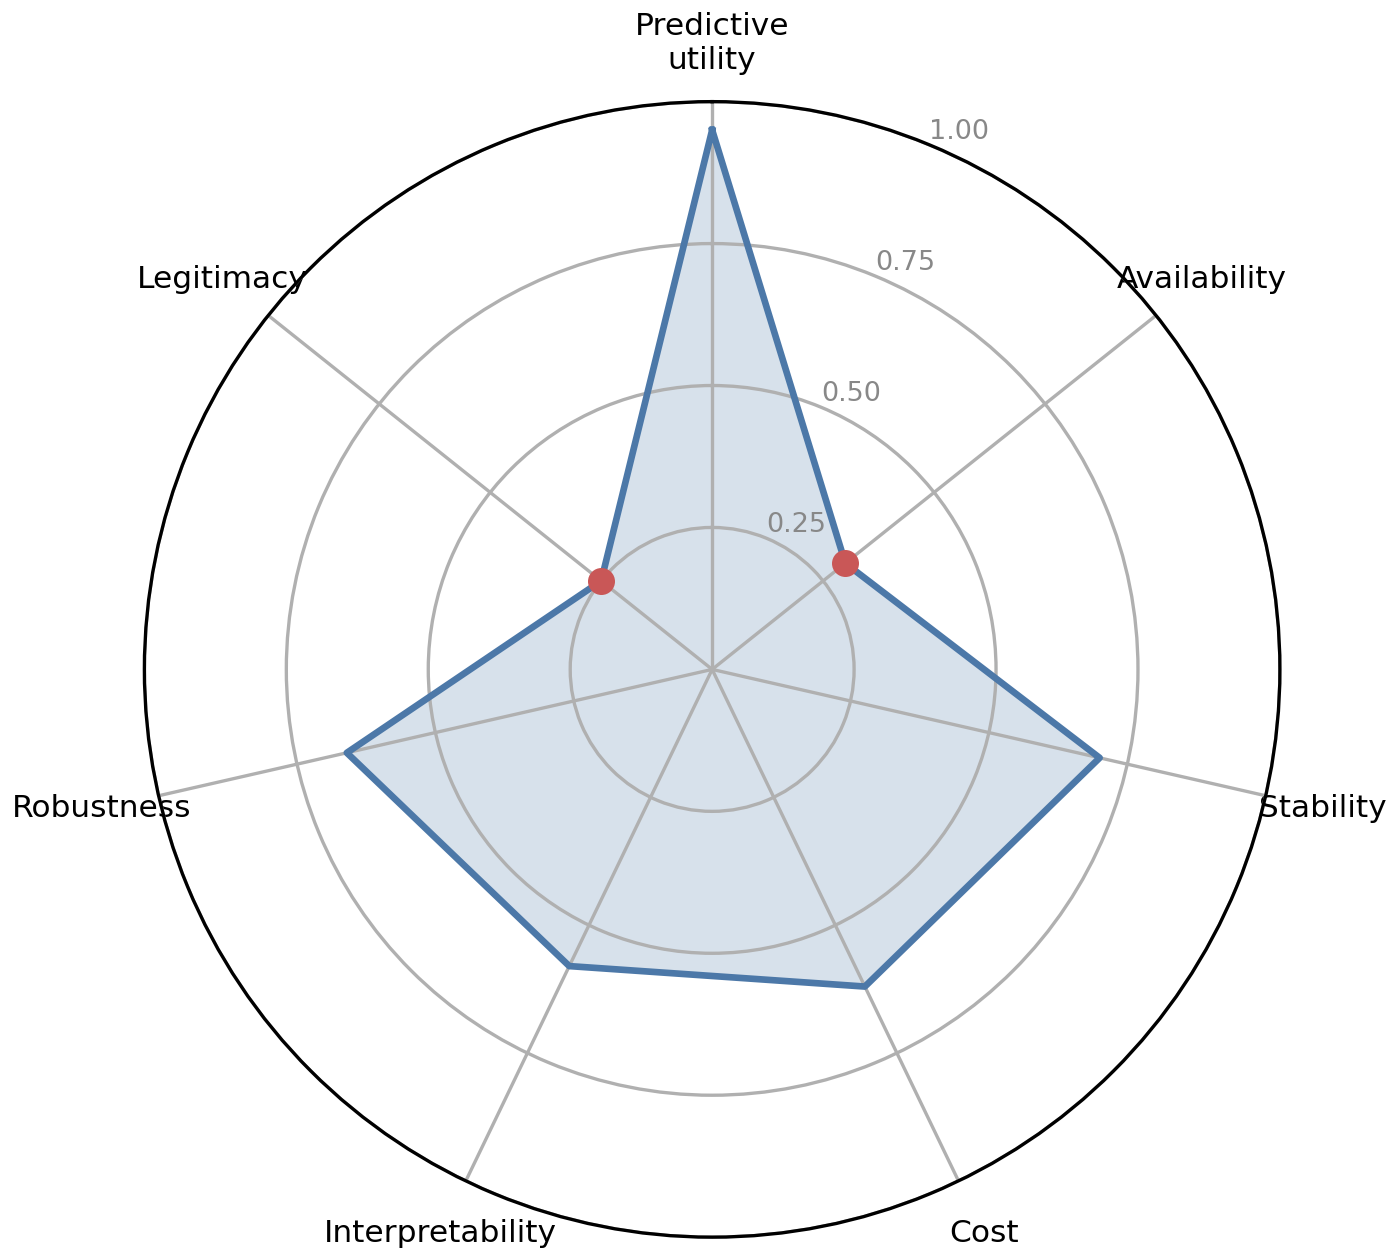
\includegraphics[width=\linewidth,height=0.72\textheight,keepaspectratio]{ch09-fig-1}
\caption{Radar Kualitas Fitur di Produksi}
\label{fig:ch09-fig-1}
\end{figure}

Pergeseran stabilitas fitur (dimensi ketiga) dapat dipantau lebih awal tanpa menunggu hasil rilis konfirmasi data (\emph{ground truth}). Metrik distribusi kuantitatif yang paling sering digunakan untuk mengukur deviasi pada variabel numerik maupun variabel kategorikal dinamakan \emph{Population Stability Index} (PSI):

\[ \text{PSI} = \sum_{i=1}^{k} (A_i - E_i) \ln \left( \frac{A_i}{E_i} \right) \]

Nilai \(A_i\) merepresentasikan proporsi populasi pada interval diskret (\emph{bin}) \(i\) ketika model beroperasi pada data produksi berjalan (\emph{actual}). Parameter \(E_i\) adalah proporsi data referensi untuk interval yang sama saat masa pelatihan model (\emph{expected}). Notasi \(k\) menunjukkan total batas pemecahan rentang observasi tersebut. Indeks PSI yang bertahan di bawah skor 0,1 mengindikasikan sebaran fitur berstatus stabil. Indeks yang melewati 0,25 menandakan distorsi pergeseran secara masif. Angka metrik pergeseran fitur ini bertindak sebagai mekanisme alarm agar model dievaluasi ulang (\emph{retraining}) untuk mencegah anomali penurunan prediksi secara tersembunyi (\emph{silent failure}).

\section{Menetapkan Baseline}\label{menetapkan-baseline}

Evaluasi kualitas fitur selalu membutuhkan titik acuan. Dalam rekayasa fitur, \emph{baseline} berfungsi sebagai batas bawah kinerja sebelum sebuah \emph{pipeline} menerima berbagai transformasi yang kompleks. Tanpa \emph{baseline}, metrik evaluasi akhir yang tinggi dapat menyesatkan; praktisi mudah menganggap bahwa penambahan fitur rumit adalah kunci tingginya akurasi, padahal model sederhana dengan data mentah bisa memberikan hasil yang serupa.

Tujuan utama menetapkan \emph{baseline} adalah mendapatkan metrik objektif untuk menguji apakah rekayasa fitur meningkatkan daya prediktif model. Proses ini umumnya mengikuti pola berikut:

\begin{itemize}
\tightlist
\item
  \textbf{Gunakan algoritma sederhana:} Hindari pencarian konfigurasi \emph{hyperparameter} atau arsitektur model yang kompleks pada tahap awal.
\item
  \textbf{Batasi pada fitur dasar:} Gunakan hanya variabel numerik asli dan variabel kategorikal yang telah melalui \emph{encoding} mendasar (misalnya \emph{one-hot encoding}).
\item
  \textbf{Terapkan \emph{dummy estimator}:} Manfaatkan alat bawaan seperti \passthrough{\lstinline!DummyClassifier!} atau \passthrough{\lstinline!DummyRegressor!} di pustaka scikit-learn. Estimator ini merekam kekuatan prediktif murni dari distribusi target tanpa mempelajari pola dari fitur sama sekali.
\end{itemize}

Sebagai contoh, pada kasus regresi, sebuah \emph{dummy estimator} dapat menggunakan rata-rata target latih sebagai nilai prediksi statis untuk seluruh data. Formulasinya adalah:

\[ \hat{y}_i = \frac{1}{n} \sum_{j=1}^{n} y_j \]

Di mana \(\hat{y}_i\) merupakan prediksi untuk sampel ke-\(i\), \(n\) adalah jumlah total sampel latih, dan \(y_j\) adalah nilai target aktual pada sampel ke-\(j\). Nilai eror dari rumusan statis ini menetapkan lantai performa yang harus dikalahkan oleh representasi fitur baru.

\begin{figure}[htbp]\centering
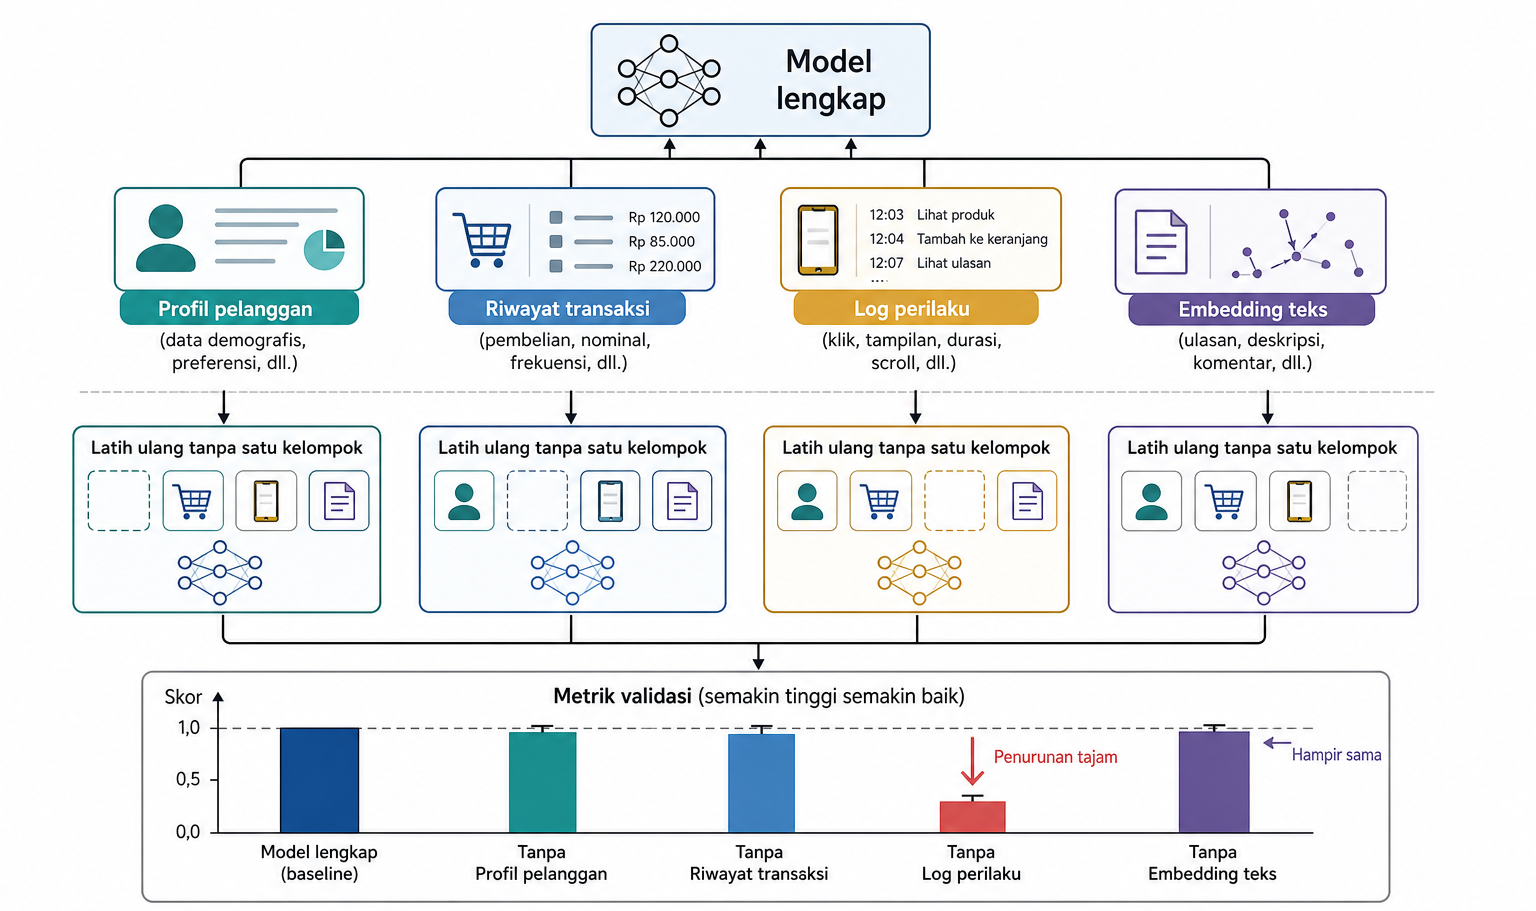
\includegraphics[width=\linewidth,height=0.72\textheight,keepaspectratio]{ch09-fig-2}
\caption{Perbandingan Utilitas Prediktif (Korelasi) vs Hubungan Kausal}
\label{fig:ch09-fig-2}
\end{figure}

Setelah \emph{baseline} tercatat, ia menjadi tolok ukur pengujian langsung untuk setiap komponen fitur turunan. Jika sebuah fitur baru mampu mengalahkan \emph{baseline}, pertanyaannya beralih: apakah margin peningkatannya sepadan dengan beban teknisnya? Beban operasional yang ditimbulkan mencakup:

\begin{itemize}
\tightlist
\item
  \textbf{Alokasi memori:} Matriks fitur berdimensi tinggi atau \emph{embedding} memakan lebih banyak kapasitas memori dan penyimpan.
\item
  \textbf{Latensi inferensi:} Pemrosesan \emph{pipeline} yang panjang memperlambat waktu respons model saat memprediksi data baru.
\item
  \textbf{Pemeliharaan kode:} Transformasi kustom menuntut pemeliharaan berkelanjutan untuk mencegah kerusakan sistem di masa depan.
\end{itemize}

Angka acuan dari \emph{baseline} ini menjadi prasyarat sebelum melangkah ke diagnosis lanjutan. Studi ablasi maupun metode atribusi seperti SHAP sepenuhnya bergantung pada metrik acuan ini untuk menghitung seberapa besar performa yang murni disumbangkan oleh fitur, bukan sekadar kebetulan dari distribusi data aslinya.

\section{\texorpdfstring{Studi \emph{Ablation}}{Studi Ablation}}\label{studi-ablation}

Studi \emph{ablation} (ablasi) adalah metode eksperimental sistematis yang dirancang untuk mengevaluasi besaran kontribusi fitur terhadap performa model secara makro. Teknik ini mengeksekusi pembuangan komponen tertentu dari data latih secara terstruktur, lalu mengukur pelemahan performa yang terjadi. Dalam konteks rekayasa fitur, ablasi umumnya dijalankan pada tingkat kelompok fitur (\emph{feature group}) alih-alih fitur tunggal individual dengan alasan operasional berikut:

\begin{itemize}
\tightlist
\item
  \textbf{Menghindari Substitusi Korelasi:} Jika hanya satu atribut yang dicabut, model (terutama model berbasis pohon ensemble) dapat memindahkan pembobotannya secara mudah ke fitur lain yang sangat berkorelasi, menciptakan ilusi bahwa atribut yang dicabut tidak berharga. Dengan menghapus seluruh kelompok semantik sekaligus (misalnya, seluruh vektor \emph{embedding} teks atau seluruh turunan agregasi log transaksi), kita memutus akses model terhadap domain informasi tersebut secara utuh.
\item
  \textbf{Efisiensi Komputasi:} Mengablasikan fitur satu per satu dari matriks berdimensi tinggi mewajibkan model dilatih ulang hingga ribuan kali, yang secara anggaran komputasi sangat tidak efisien.
\end{itemize}

Siklus pengujian ablasi mengikuti protokol eksperimen yang presisi:

\begin{enumerate}
\def\labelenumi{\arabic{enumi}.}
\tightlist
\item
  Melatih model menggunakan himpunan data lengkap untuk menetapkan metrik performa maksimal sebagai \emph{baseline}.
\item
  Memangkas satu kelompok fitur spesifik dari himpunan data.
\item
  Melatih ulang model menggunakan sisa himpunan fitur.
\item
  Menghitung delta (selisih) performa model terablasi terhadap \emph{baseline} guna memverifikasi besaran utilitas absolut kelompok tersebut. Penurunan utilitas ini dapat dirumuskan sebagai:
  \[ \Delta \mathcal{M}_{G} = \mathcal{M}(F_{\text{all}}) - \mathcal{M}(F_{\text{all}} \setminus G) \]
  Di mana \(\Delta \mathcal{M}_{G}\) melambangkan penurunan skor performa akibat pencabutan kelompok fitur \(G\), \(\mathcal{M}\) melambangkan fungsi metrik evaluasi model (seperti akurasi atau AUC), dan \(F_{\text{all}}\) adalah himpunan total seluruh fitur dasar.
\end{enumerate}

Sebagai ilustrasi praktis pada klasifikasi deteksi penipuan (\emph{fraud detection}), membuang seluruh kelompok fitur ``riwayat agregasi transaksi'' dapat menjatuhkan metrik \emph{Area Under the Curve} (AUC) hingga 5\%, yang membuktikan tingginya nilai prediktif kelompok tersebut. Sebaliknya, apabila ``demografi geografis pengguna'' dipangkas namun performa AUC stabil, rekayasawan memperoleh justifikasi kuantitatif untuk menghapus fitur tersebut. Pemangkasan ini esensial untuk menurunkan latensi \emph{inference} dan mengurangi beban rekayasa perangkat lunak.

Walaupun studi ablasi efektif sebagai saringan domain awal, teknik ini tidak didesain untuk merinci mana variabel yang paling vital \emph{di dalam} sebuah kelompok. Untuk melakukan pemeringkatan fitur tingkat mikro, pengujian ini harus diteruskan dengan \emph{permutation importance} atau atribusi SHAP.

\section{\texorpdfstring{\emph{Permutation} dan \emph{Model-Based Importance}}{Permutation dan Model-Based Importance}}\label{permutation-dan-model-based-importance}

Evaluasi kualitas fitur secara individual bertumpu pada dua pendekatan utama: \emph{model-based importance} dan \emph{permutation importance}. Keduanya mengukur kontribusi sebuah fitur terhadap daya prediksi algoritma, tetapi beroperasi dengan mekanisme dan kelemahan evaluasi yang berbeda.

Pendekatan \emph{model-based importance} menghitung utilitas fitur bersamaan dengan proses pelatihan. Pada keluarga algoritma pohon keputusan, skor dihitung berdasarkan frekuensi dan efektivitas sebuah fitur saat memecah data. Pendekatan ini memiliki dua karakteristik utama:

\begin{itemize}
\tightlist
\item
  \textbf{Komputasi efisien:} Penilaian terintegrasi langsung ke dalam eksekusi fase pelatihan, sehingga tidak menuntut iterasi komputasi tambahan.
\item
  \textbf{Bias kardinalitas:} Evaluasi internal merespons \emph{overfitting} pada fitur yang memiliki variasi nilai unik tinggi (kardinalitas tinggi). Jika matriks memiliki kolom ID pelanggan, algoritma akan mengeksploitasi nilai ID tersebut untuk menghafal target kelas. Kolom ID menempati peringkat atas meskipun tidak membawa sinyal prediktif general.
\end{itemize}

Untuk algoritma berbasis pohon, kontribusi fitur dihitung dari akumulasi penurunan \emph{impurity} (ketidakmurnian). Jika algoritma menggunakan \emph{Gini impurity}, penurunannya pada sebuah titik pemecahan (\emph{node}) diformulasikan sebagai:

\[ \Delta I = I_{\text{parent}} - \left( \frac{N_{\text{left}}}{N} I_{\text{left}} + \frac{N_{\text{right}}}{N} I_{\text{right}} \right) \]

Di mana \(I_{\text{parent}}\) adalah nilai ketidakmurnian sebelum pemecahan, \(N\) adalah total observasi pada \emph{node} induk, sedangkan \(N_{\text{left}}\) dan \(N_{\text{right}}\) mewakili jumlah observasi pada cabang kiri dan kanan beserta nilai ketidakmurniannya masing-masing (\(I_{\text{left}}\) dan \(I_{\text{right}}\)). Fitur yang berulang kali menghasilkan \(\Delta I\) terbesar menerima bobot \emph{importance} tertinggi.

Pendekatan alternatif yang lebih objektif adalah \emph{permutation importance}. Metode ini bersifat \emph{model-agnostic} (berlaku untuk semua algoritma) dan dieksekusi setelah model selesai dilatih. Evaluasi wajib dijalankan menggunakan data validasi independen untuk menghindari bias hafalan dari data latih.

Prosedur \emph{permutation importance} bekerja melalui tahapan berikut:

\begin{enumerate}
\def\labelenumi{\arabic{enumi}.}
\tightlist
\item
  Model mengeksekusi prediksi awal pada himpunan data validasi untuk mencatat skor performa referensi (\emph{baseline}).
\item
  Susunan nilai pada satu fitur spesifik diacak antar-baris, sementara kolom fitur lainnya dibiarkan utuh. Pengacakan ini memutus tautan informasi antara fitur tersebut dengan variabel target.
\item
  Model memprediksi ulang himpunan data yang telah teracak sebagian.
\item
  Fitur dikategorikan esensial jika intervensi pengacakan membuat tingkat galat model melonjak tajam melewati skor \emph{baseline}. Jika akurasi model tetap stabil, fitur tersebut terkonfirmasi tidak memiliki daya prediktif.
\end{enumerate}

\begin{figure}[htbp]\centering
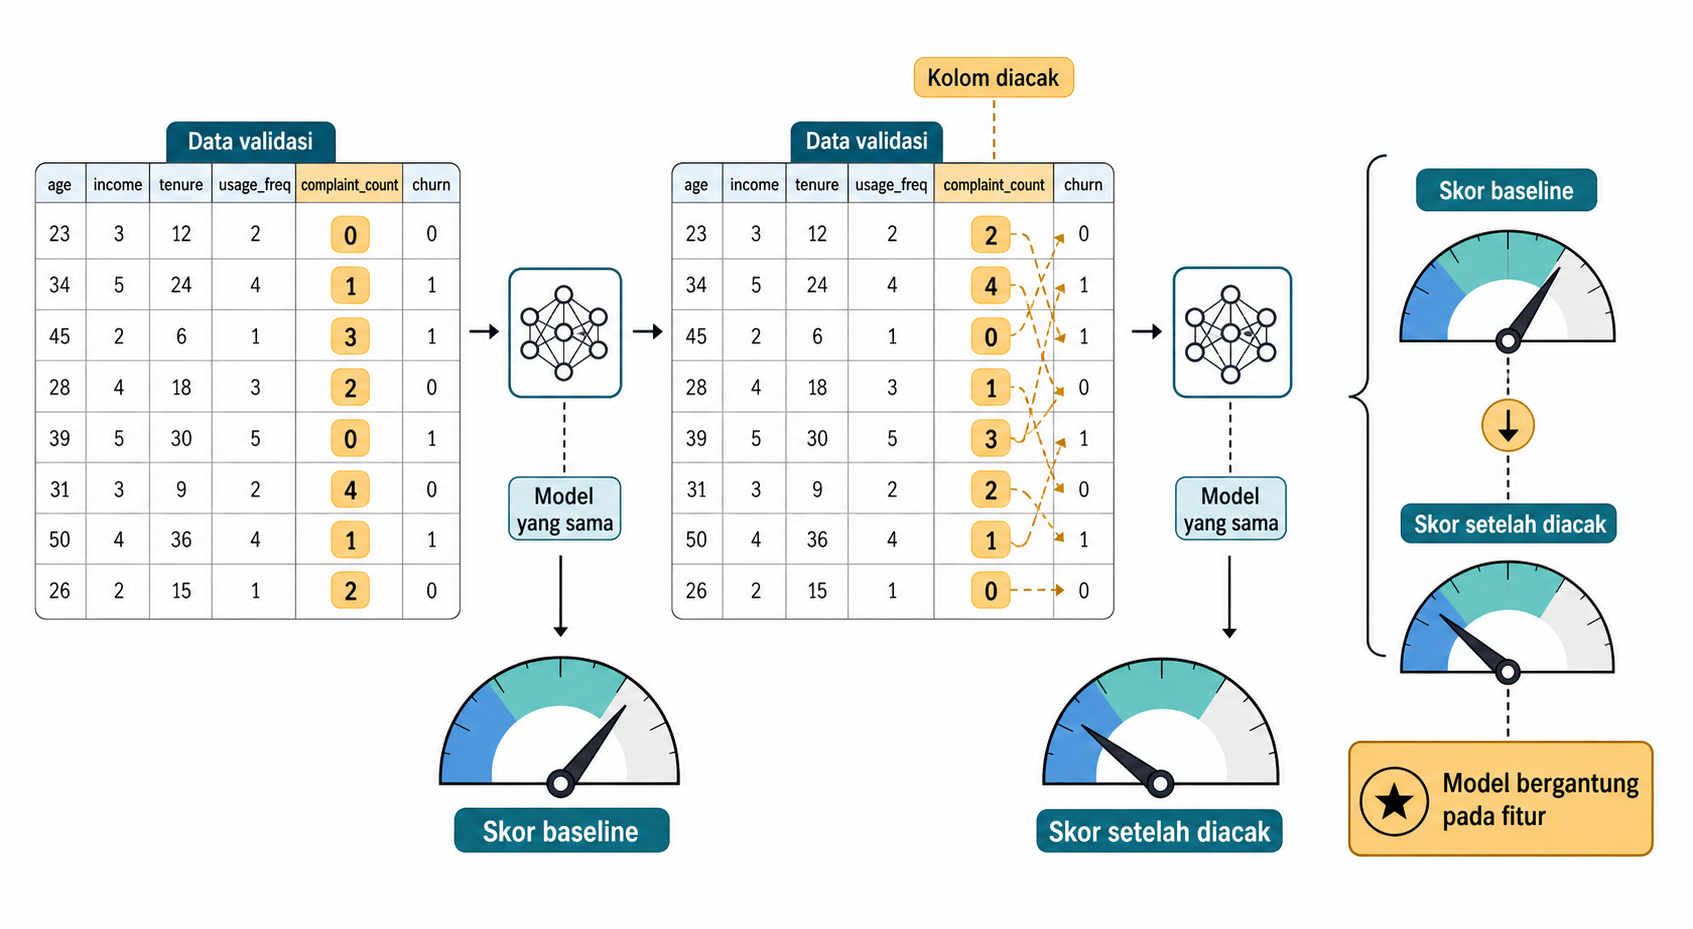
\includegraphics[width=\linewidth,height=0.72\textheight,keepaspectratio]{ch09-fig-3}
\caption{Alur Kebocoran Atribut Sensitif Lewat Fitur Proksi dan Embedding}
\label{fig:ch09-fig-3}
\end{figure}

Walaupun kebal terhadap \emph{overfitting} kardinalitas, \emph{permutation importance} konvensional kehilangan akurasi saat mengukur fitur yang saling berkorelasi. Ketika dua fitur mengandung informasi yang tumpang tindih (misalnya luas lahan dan luas bangunan), mengacak salah satu fitur tidak memicu penurunan performa drastis. Model masih bisa mengekstrak sinyal prediktif yang sama dari fitur pasangannya yang utuh. Akibatnya, skor kedua fitur tersebut dilaporkan jauh lebih rendah dari kontribusi aslinya. Untuk mengatasi penalti korelasi ini, varian analitis seperti \emph{Conditional Permutation Importance} (CPI) mengacak nilai fitur mengikuti distribusi kondisionalnya, sehingga struktur korelasi gabungan dalam matriks tetap terjaga.

\section{SHAP untuk Diagnosis Fitur}\label{shap-untuk-diagnosis-fitur}

Metode \emph{permutation importance} memetakan utilitas prediktif secara global, tetapi tidak memadai ketika praktisi perlu menjelaskan mengapa model menghasilkan satu keputusan spesifik pada satu observasi data. Untuk menjawab kebutuhan diagnostik mikro ini, kerangka kerja SHAP (\emph{SHapley Additive exPlanations}) telah menjadi standar industri dalam mengevaluasi atribusi fitur.

Secara matematis, SHAP mengadopsi aksioma dari teori permainan kooperatif (\emph{cooperative game theory}) untuk menghitung bobot nilai (\emph{Shapley values}) melalui persamaan:
\[ \phi_j(x) = \sum_{S \subseteq F \setminus \{j\}} \frac{|S|! (|F| - |S| - 1)!}{|F|!} \left[ v_x(S \cup \{j\}) - v_x(S) \right] \]
Di mana \(\phi_j\) merupakan nilai SHAP untuk atribut ke-\(j\), \(F\) adalah total himpunan atribut (fitur), \(S\) merepresentasikan subset fitur spesifik yang sedang dievaluasi dari model, dan \(v_x(S)\) adalah keluaran model saat hanya mempertimbangkan kombinasi fitur di dalam \(S\).

Metode ini dibangun di atas pilar analitik berikut:

\begin{itemize}
\tightlist
\item
  \textbf{Pemain dan \emph{Payout}:} Prediksi model diposisikan sebagai hasil akhir permainan (\emph{payout}), sementara setiap fitur adalah pemain (\emph{player}) yang bekerja sama membentuk hasil tersebut.
\item
  \textbf{Sifat Aditif:} Algoritma secara adil mendistribusikan selisih antara tebakan observasi tunggal dengan \emph{baseline} (rata-rata prediksi model pada seluruh populasi latih). Penjumlahan seluruh skor atribusi fitur (ditambah nilai \emph{baseline}) akan selalu setara dengan angka keluaran model.
\item
  \textbf{Vektor Arah dan Interaksi:} Berbeda dengan metrik global yang hanya menghasilkan magnitudo absolut, SHAP menangkap arah dampak (\emph{directional effect}) secara lokal. Sebagai contoh, atribut ``usia \textgreater{} 50 tahun'' mungkin mengerek probabilitas risiko Pasien A sebesar +12\%, namun menurunkannya -2\% pada Pasien B karena SHAP memperhitungkan efek interaksi fitur usia tersebut dengan riwayat penyakit pasien yang bersangkutan.
\end{itemize}

Transparansi tingkat granular ini mengubah nilai komputasi mentah menjadi diagnosis yang dapat diaudit. Apabila sebuah model klasifikasi menolak pengajuan kredit pelanggan, nilai lokal SHAP memaparkan rincian vektor gaya yang saling berlawanan: probabilitas penolakan didorong naik secara dominan oleh ``rasio utang yang tinggi'', dan ditahan turun oleh ``durasi nasabah yang lama''.

\begin{figure}[htbp]\centering
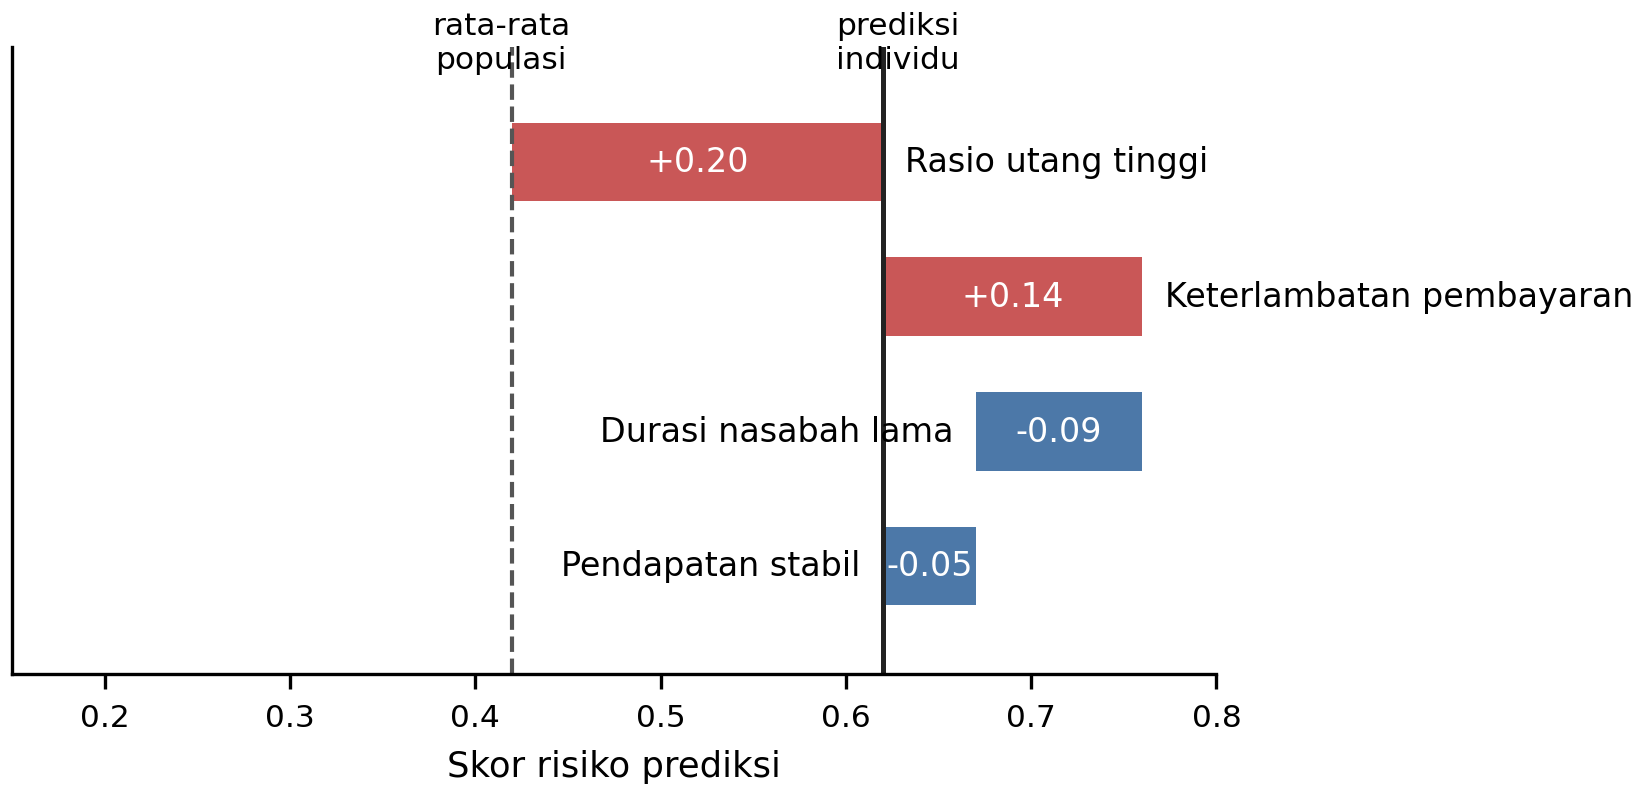
\includegraphics[width=\linewidth,height=0.72\textheight,keepaspectratio]{ch09-fig-4}
\caption{Integrasi Metadata Data Card dan Silsilah Fitur pada Feature Store}
\label{fig:ch09-fig-4}
\end{figure}

Lebih jauh, penjelasan lokal ini dapat diagregasi kembali menjadi wawasan global. Praktik mutakhir dalam rekayasa fitur mulai mengadopsi rata-rata absolut nilai SHAP (\(\text{mean}(|\text{SHAP}|)\)) melintasi seluruh himpunan data sebagai kriteria utama untuk menyaring variabel, melahirkan perangkat \emph{pipeline} hibrida seperti \emph{BorutaShap}. Analisis distribusi nilai SHAP memungkinkan rekayasawan mendeteksi area non-linearitas, memvalidasi asumsi mekanis, serta membuktikan kepada pemangku kepentingan bahwa representasi data yang dirancang bekerja secara rasional.

\section{\texorpdfstring{Stabilitas Lintas \emph{Fold} dan Ilusi Kausalitas}{Stabilitas Lintas Fold dan Ilusi Kausalitas}}\label{stabilitas-lintas-fold-dan-ilusi-kausalitas}

Mengevaluasi kualitas fitur sering memunculkan dua asumsi keliru. Asumsi pertama adalah mempercayai skor evaluasi secara absolut dari satu partisi data tunggal. Asumsi kedua adalah mencampuradukkan kemampuan prediktif model dengan hubungan sebab-akibat di dunia nyata.

\textbf{Stabilitas Skor Kepentingan.}\label{stabilitas-skor-kepentingan}

Mengukur \emph{feature importance} menggunakan satu set pelatihan dan set pengujian tunggal membuat evaluasi rentan terhadap variansi sampel. Sebuah fitur dapat terlihat dominan secara kebetulan karena distribusi data yang tidak berimbang atau keberadaan nilai pencilan di dalam partisi spesifik tersebut.

Pengujian ketahanan fitur mengharuskan kita menguji stabilitas skor kepentingan di seluruh iterasi \emph{cross-validation}. Fluktuasi ini dievaluasi secara matematis melalui perhitungan varians skor:

\[ \text{Var}(I_j) = \frac{1}{K-1} \sum_{k=1}^K (I_{j,k} - \bar{I}_j)^2 \]

Di mana \(K\) adalah total \emph{fold} dalam \emph{cross-validation}, \(I_{j,k}\) adalah skor \emph{feature importance} untuk fitur \(j\) pada \emph{fold} ke-\(k\), dan \(\bar{I}_j\) merupakan rata-rata skor kepentingan pada seluruh \emph{fold}.

Varians yang tinggi memperlihatkan bahwa model menghafal pola acak pada iterasi pelatihan tertentu. Fitur dengan nilai kepentingan menengah tetapi konsisten jauh lebih menjamin kemampuan generalisasi model dibandingkan fitur yang mencatatkan skor puncak namun fluktuatif.

Evaluasi stabilitas ini mendapat tantangan tambahan saat menghadapi fitur yang saling berkorelasi:

\begin{itemize}
\tightlist
\item
  \textbf{Kelemahan Permutasi Marginal:} \emph{Permutation importance} standar mengacak nilai observasi secara marginal. Jika fitur A dan B berkorelasi kuat lalu A diacak, model masih dapat mengambil informasi dari B. Kedua fitur tersebut pada akhirnya mendapatkan skor yang lebih rendah dari kontribusi aslinya.
\item
  \textbf{Pengacakan Bersyarat (CPI):} Teknik modern seperti \emph{Conditional Permutation Importance} (CPI) mengacak data berbasis distribusi kondisional. Metode ini mempertahankan struktur korelasi antar-fitur sehingga ukuran tingkat kepentingan tetap akurat.
\item
  \textbf{Kestabilan Seleksi:} Algoritma seleksi seperti Boruta-SHAP sering dimanfaatkan untuk menekan angka varians ini, menstabilkan hasil \emph{feature importance} melalui kombinasi permutasi label target.
\end{itemize}

\textbf{Membedakan Utilitas Prediktif dan Efek Kausal.}\label{membedakan-utilitas-prediktif-dan-efek-kausal}

Skor \emph{feature importance} yang tinggi kerap memancing dugaan bahwa fitur tersebut adalah penyebab fenomena target. Ukuran ini pada dasarnya hanya mengkuantifikasi korelasi matematis untuk meminimalkan galat, bukan mengungkap kausalitas.

Sebagai ilustrasi, sebuah algoritma dilatih memprediksi angka kecelakaan lalu lintas harian menggunakan berbagai data atribut kota. Fitur volume penjualan payung mungkin keluar dengan tingkat \emph{feature importance} paling tinggi. Model menangkap kecocokan statistik: saat grafik penjualan payung menanjak, frekuensi kecelakaan juga tinggi.

Menerbitkan peraturan pelarangan toko menjual payung tidak akan menurunkan jumlah kecelakaan jalan raya. Penjualan payung dan kecelakaan lalu lintas didorong oleh variabel perancu eksternal yang sama, yaitu turunnya hujan. Model mengeksploitasi korelasi ini murni karena datanya tersedia dan berpola stabil.

Interpretasi skor fitur selalu bergantung pada orientasi operasional \emph{pipeline}:

\begin{itemize}
\tightlist
\item
  \textbf{Peramalan:} Jika sasaran utama model sebatas memprediksi lonjakan pasien untuk menyiapkan ruang gawat darurat, menyertakan atribut penjualan payung tetap menjadi strategi yang valid.
\item
  \textbf{Intervensi:} Jika sasarannya menekan angka kecelakaan melalui intervensi kebijakan (perspektif yang dibahas di Bab 17), modifikasi pada atribut prediktif non-kausal sama sekali tidak memberikan dampak nyata.
\end{itemize}

Ketika \emph{pipeline} dirancang untuk mengambil tindakan intervensi, skor \emph{feature importance} standar harus diganti. Literatur analitik mengembangkan kerangka terpisah untuk persoalan ini:

\begin{itemize}
\tightlist
\item
  \textbf{Double/Debiased Machine Learning (DML):} Teknik ini memisahkan tugas prediksi dan estimasi efek kausal melalui tahap pembagian sampel silang. Model \emph{machine learning} difungsikan untuk menghapus pengaruh variabel perancu terlebih dahulu sebelum dampak kausal dari suatu fitur dievaluasi.
\item
  \textbf{Causal Forest:} Berbeda dengan analisis reduksi galat murni, varian algoritma ini memformulasikan nilai \emph{variable importance} spesifik untuk mengukur seberapa besar sebuah atribut memengaruhi tingkat heterogenitas efek perlakuan (perbedaan respons lintas subpopulasi).
\end{itemize}

\section{Informasi Sensitif dan Fitur Proksi}\label{informasi-sensitif-dan-fitur-proksi}

Evaluasi fitur yang utuh wajib mengukur utilitas prediktif sekaligus memperhitungkan batas privasi dan keadilan (\emph{fairness}). Praktik awal umumnya menerapkan \emph{fairness through unawareness}, yaitu secara langsung menghapus atribut sensitif (seperti ras, gender, atau status medis) dari \emph{dataset}. Namun, menghilangkan kolom identitas tidak dengan sendirinya menuntaskan masalah bias. Model tetap dapat membedakan kelompok demografis dan menghasilkan keputusan yang diskriminatif melalui fitur-fitur perantara.

\emph{Proxy feature} (fitur proksi) adalah variabel yang tampak netral secara harfiah, tetapi memiliki korelasi statistik yang tinggi dengan atribut sensitif. Jika model mempelajari pola dari fitur proksi, model akan merekonstruksi identitas pengguna dan mengulang pola bias historis.

Karakteristik penyusupan proksi umumnya terjadi melalui:

\begin{itemize}
\tightlist
\item
  \textbf{Kode pos wilayah hunian:} Secara fungsional merepresentasikan titik geografis, tetapi distribusinya sering mencerminkan pembelahan strata sosial ekonomi dan demografi kelompok tertentu.
\item
  \textbf{Tipe perangkat pintar:} Riwayat pemakaian gawai tertentu atau catatan kunjungan gerai memiliki korelasi yang kuat dengan parameter kelas pendapatan.
\item
  \textbf{Representasi laten (\emph{embedding}):} Pada pengolahan teks atau citra, vektor kontinu (\emph{embedding}) memampatkan data mentah menjadi representasi numerik berdimensi tinggi. Vektor ini ikut merekam dialek, struktur kalimat, atau preferensi yang mengarah langsung ke usia dan gender penggunanya. Karena dimensi \emph{embedding} sulit dibaca oleh mata manusia, informasi sensitif dapat menembus inspeksi keamanan secara terselubung.
\end{itemize}

{[}GAMBAR 9.X: Skema - Alur kebocoran atribut sensitif ke dalam model melalui korelasi fitur proksi dan dimensi embedding{]}

\textbf{Mempertahankan Atribut untuk Audit}

Penghapusan atribut identitas sejak awal persiapan data justru memunculkan hambatan struktural pada saat validasi. Pengembang akan kesulitan membuktikan secara objektif apakah sekumpulan fitur mendiskriminasi usia atau ras tertentu apabila data acuan tersebut sudah dihilangkan.

Skenario audit modern menyarankan pemisahan strategi: atribut sensitif dipertahankan utuh di dalam \emph{dataset} pengujian murni untuk mengakomodasi pengukuran bias. Mengukur disaggregasi keadilan dengan data yang nyata membuahkan hasil pengujian yang transparan, jauh lebih baik dibandingkan menghapus kolom aslinya dan sekadar berasumsi bahwa tidak ada efek proksi yang terjadi.

\textbf{Prinsip Minimisasi Data}

Fakta bahwa penambahan fitur dapat menaikkan metrik performa model tidak memberikan legitimasi etis untuk selalu menggunakannya. Cara utama memitigasi bahaya privasi adalah dengan menerapkan \emph{data minimization}. Sistem \emph{machine learning} dituntut hanya memproses fitur yang esensial untuk tugas prediksi.

Dalam tahapan seleksi representasi, konsep minimisasi ini dapat diformalkan dengan memasukkan penalti kompleksitas (\emph{complexity penalty}) ke dalam fungsi evaluasi. Pencarian tidak lagi hanya berfokus pada reduksi galat, melainkan ikut memaksakan penalti atas bertambahnya ukuran atau kerentanan fitur:

\[ 
\text{Objektif} = \text{Galat}(\hat{Y}, Y) + \lambda \sum_{j=1}^{p} c_j 
\]

Di mana \(\text{Galat}(\hat{Y}, Y)\) adalah deviasi prediksi model terhadap label target yang sebenarnya, \(\lambda\) adalah parameter yang mengatur kekuatan penalti, dan \(c_j\) melambangkan bobot biaya (atau tingkat risiko privasi) dari fitur ke-\(j\).

\begin{itemize}
\tightlist
\item
  \textbf{Pemisahan akurasi dan kelayakan etis:} Peningkatan nilai akurasi tidak boleh dicapai dengan mengorbankan keamanan data pengguna. Model dengan selisih akurasi marjinal sering kali lebih aman jika dilatih dengan kelompok fitur yang lebih terisolasi dari bias.
\item
  \textbf{Inspeksi berlapis:} Praktisi diwajibkan memvalidasi bahwa angka presisi yang tinggi didapatkan dari sinyal yang sah, bukan dari eksploitasi celah identitas demografis.
\end{itemize}

Aturan minimisasi dan verifikasi stabilitas ini merupakan standar perancangan yang akan dirujuk kembali ketika seluruh tahapan dipadukan menjadi sebuah \emph{pipeline} utuh pada fase produksi.

\section{Mendokumentasikan Keputusan Fitur}\label{mendokumentasikan-keputusan-fitur}

Fase eksperimen \emph{machine learning} menghasilkan puluhan hingga ratusan fitur baru. Tanpa pencatatan sistematis, tumpukan fitur ini berubah menjadi beban teknis. Praktisi yang menjumpai variabel seperti \passthrough{\lstinline!skor_aktivitas_terbobot!} di dalam basis kode sering tidak mengetahui asal data, metode perhitungan, atau dampaknya jika fitur tersebut dihapus. Ketidakpastian ini menyebabkan fitur usang tetap dipertahankan di dalam \emph{pipeline}, yang pada akhirnya memperlambat komputasi dan menyulitkan pemeliharaan sistem.

Dokumentasi fitur modern mencakup informasi operasional menyeluruh, tidak hanya nama variabel dan tipe data. Praktik dokumentasi saat ini mengadaptasi tiga kerangka kerja formal dari literatur \emph{machine learning}:

\begin{itemize}
\tightlist
\item
  \textbf{Datasheets for Datasets:} Mendokumentasikan motivasi pengumpulan, komposisi label, proses prapemrosesan, dan batasan penggunaan untuk merekam silsilah (\emph{provenance}) data mentah sebelum diubah menjadi fitur.
\item
  \textbf{Model Cards:} Berisi laporan metrik evaluasi yang disagregasi berdasarkan kelompok demografis. Pada level fitur, format ini memastikan performa dipecah untuk mendeteksi keberadaan fitur proksi.
\item
  \textbf{Data Cards:} Menggunakan skema berlapis (\emph{telescopic}, \emph{periscopic}, \emph{microscopic}) untuk menangkap alasan pembuatan fitur, evolusi transformasi, dan rekam jejak operasionalnya.
\end{itemize}

{[}GAMBAR 9.8: Diagram - Integrasi Metadata Data Card dan Silsilah Fitur pada Feature Store{]}

Dalam arsitektur produksi, metadata dokumentasi dipusatkan di dalam \emph{feature store} atau \emph{feature catalog}. Platform ini mengintegrasikan definisi, identitas pemilik (\emph{owner}), silsilah data (\emph{lineage}), dan metrik kebaruan data (\emph{freshness}). Integrasi langsung dengan repositori kode membuat fitur terdokumentasi secara bawaan dan siap digunakan ulang lintas model.

Sebuah catatan keputusan fitur yang komprehensif memuat empat elemen utama:

\begin{enumerate}
\def\labelenumi{\arabic{enumi}.}
\tightlist
\item
  \textbf{Definisi dan Logika Bisnis:} Alasan fitur dirancang dan sinyal spesifik yang ingin diekstraksi dari data mentah.
\item
  \textbf{Transformasi dan Asumsi Operasional:} Aturan matematis eksplisit yang diterapkan, seperti metode imputasi nilai kosong, batas pemotongan \emph{outlier}, atau teknik penskalaan.
\item
  \textbf{Sumber Data dan Lineage:} Silsilah lengkap dari tabel basis data awal hingga menjadi matriks fitur akhir. Informasi ini menjamin konsistensi logika transformasi antara fase pelatihan dan \emph{inference}.
\item
  \textbf{Dampak Kuantitatif terhadap Baseline:} Bukti empiris bahwa fitur memberikan peningkatan performa yang melampaui biaya pemrosesannya. Catatan merekam hasil uji ablasinya, misalnya metrik peningkatan skor AUC sebesar 0,04 dibandingkan performa model dasar tanpa fitur tersebut.
\end{enumerate}

Pencatatan terstruktur mengeliminasi duplikasi eksperimen. Tim pengembangan dapat merujuk pada histori dokumentasi untuk mengetahui pendekatan ekstraksi yang telah diuji namun gagal, tanpa harus menjalankan ulang skrip pelatihan atau membongkar kode sumber baris demi baris. Buku ini menyediakan templat operasional dokumentasi fitur berdasarkan keempat elemen tersebut pada Lampiran C.

\section{Studi Kasus: Ablation Lintas Kelompok Fitur}\label{studi-kasus-ablation-lintas-kelompok-fitur}

Sebagai studi kasus, kita mengevaluasi fitur pada model klasifikasi risiko kredit. Dataset terdiri atas tiga kelompok fitur:

\begin{itemize}
\tightlist
\item
  \textbf{Demografis:} rentang usia dan wilayah tempat tinggal.
\item
  \textbf{Riwayat transaksi:} agregasi keterlambatan bayar dan total pengeluaran finansial.
\item
  \textbf{Log interaksi:} jejak klik aplikasi dan durasi sesi pengguna.
\end{itemize}

Evaluasi dimulai dengan melatih model menggunakan seluruh fitur untuk menetapkan skor \emph{baseline}. Studi \emph{ablation} kemudian mengevaluasi setiap kelompok fitur dengan cara mencabutnya dari \emph{pipeline} pelatihan satu per satu. Dampak pencabutan fitur ini diformulasikan sebagai selisih performa:

\[ \Delta \mathcal{M}_{g} = \mathcal{M}(F_{all}) - \mathcal{M}(F_{all} \setminus g) \]

Di mana \(\Delta \mathcal{M}_{g}\) adalah perubahan performa akibat pencabutan kelompok fitur \(g\), \(\mathcal{M}\) mewakili metrik evaluasi seperti akurasi atau \emph{Area Under Curve} (AUC), \(F_{all}\) adalah set fitur \emph{baseline}, dan \(F_{all} \setminus g\) merupakan set fitur tanpa kelompok \(g\).

Pengujian \emph{ablation} menghasilkan observasi berikut:

\begin{itemize}
\tightlist
\item
  \textbf{Pencabutan demografis (\(\Delta \mathcal{M} \approx 0\)):} Performa model tetap stabil. Profil risiko kredit lebih banyak dijelaskan oleh perilaku keuangan daripada atribut statis, sehingga fitur demografis dapat dibuang tanpa kerugian prediktif.
\item
  \textbf{Pencabutan riwayat transaksi (\(\Delta \mathcal{M} \gg 0\)):} Akurasi model turun tajam. Penurunan ini mengonfirmasi bahwa riwayat transaksi merupakan sinyal utama prediksi yang wajib dipertahankan.
\item
  \textbf{Pencabutan log interaksi (\(\Delta \mathcal{M} > 0\), bernilai kecil):} Akurasi berkurang sedikit, tetapi pemrosesan log bervolume besar memakan komputasi tinggi. Mempertahankan fitur ini akan menaikkan \emph{latency} pada tahap \emph{inference}.
\end{itemize}

{[}GAMBAR 9.5: Diagram Batang - Perbandingan skor metrik baseline dengan skor setelah setiap kelompok fitur dicabut (demografis, transaksi, log interaksi){]}

Stabilitas skor dievaluasi lebih lanjut menggunakan \emph{cross-validation} untuk memastikan hasil tidak bias terhadap satu irisan data. Hasil uji konsisten di setiap \emph{fold}: fitur transaksi selalu memicu penurunan skor yang besar saat dihilangkan, sementara fitur log dan demografis berdampak minimal.

Desain arsitektur final memutuskan untuk mempertahankan riwayat transaksi finansial dan membuang fitur lainnya. Keputusan ini mempertimbangkan keseimbangan antara daya prediksi model, biaya komputasi, dan kebutuhan \emph{latency} sistem di lingkungan produksi.

% ==========================================================================
% ch10.tex — dihasilkan otomatis dari website/chapters/ch10.qmd
% Boleh disunting manual. 'sync' hanya menimpa bila .qmd berubah DAN .tex
% belum disunting; kalau keduanya berubah, dilewati (pakai --force).
% qmd-sha1: 9357996c9227
% tex-sha1: 2e449f693a83
% ==========================================================================
% >>>>> ISI OTOMATIS (jangan hapus baris ini) >>>>>
\chapter{Deret Waktu \& Data Sensor}\label{deret-waktu-data-sensor}

\section{Konstruksi Sampel Temporal: Lookback, Stride, Horizon, dan Penyelarasan}\label{konstruksi-sampel-temporal-lookback-stride-horizon-dan-penyelarasan}

Dalam data tabular konvensional, satu baris umumnya merepresentasikan satu unit observasi yang independen. Namun, pada data deret waktu (\emph{time series}), setiap observasi terhubung oleh urutan kronologis. Baris-baris tersebut tidak dapat diambil secara acak. Untuk melatih algoritma pada data kontinu, sampel pembelajaran harus dikonstruksi melalui mekanisme \emph{windowing}.

Mekanisme \emph{windowing} mempartisi deret waktu kontinu menjadi himpunan sampel individual, di mana masing-masing memuat fitur historis sebagai masukan dan target masa depan sebagai prediksi. Proses ini dikendalikan oleh tiga parameter operasional: \emph{lookback}, \emph{horizon}, dan \emph{stride}. Parameter \emph{lookback} menentukan panjang rentang waktu historis yang digunakan model, misalnya tujuh hari riwayat penjualan untuk memprediksi hari esok. Parameter \emph{horizon} menentukan jarak waktu masa depan serta panjang target prediksi tersebut. Selanjutnya, \emph{stride} mengatur ukuran pergeseran jendela saat membentuk sampel berikutnya. Nilai \emph{stride} yang kecil akan memperbanyak jumlah sampel latih, tetapi sekaligus meningkatkan korelasi antarobservasi akibat tingginya tingkat tumpang tindih (\emph{overlapping}).

Secara matematis, untuk deret waktu \(x = \{x_1, x_2, \dots, x_T\}\), sampel historis pada titik waktu \(t\) direpresentasikan sebagai vektor jendela \(W_t = [x_{t-L+1}, x_{t-L+2}, \dots, x_t]\). Dalam formulasi ini, variabel \(W_t\) merupakan jendela input pada titik waktu \(t\) yang memiliki panjang \emph{lookback} sebesar \(L\). Jendela tersebut dipasangkan dengan target observasi \(y_{t+H}\), dengan variabel \(H\) menunjukkan jarak \emph{horizon} ke masa depan.

\begin{figure}[htbp]\centering
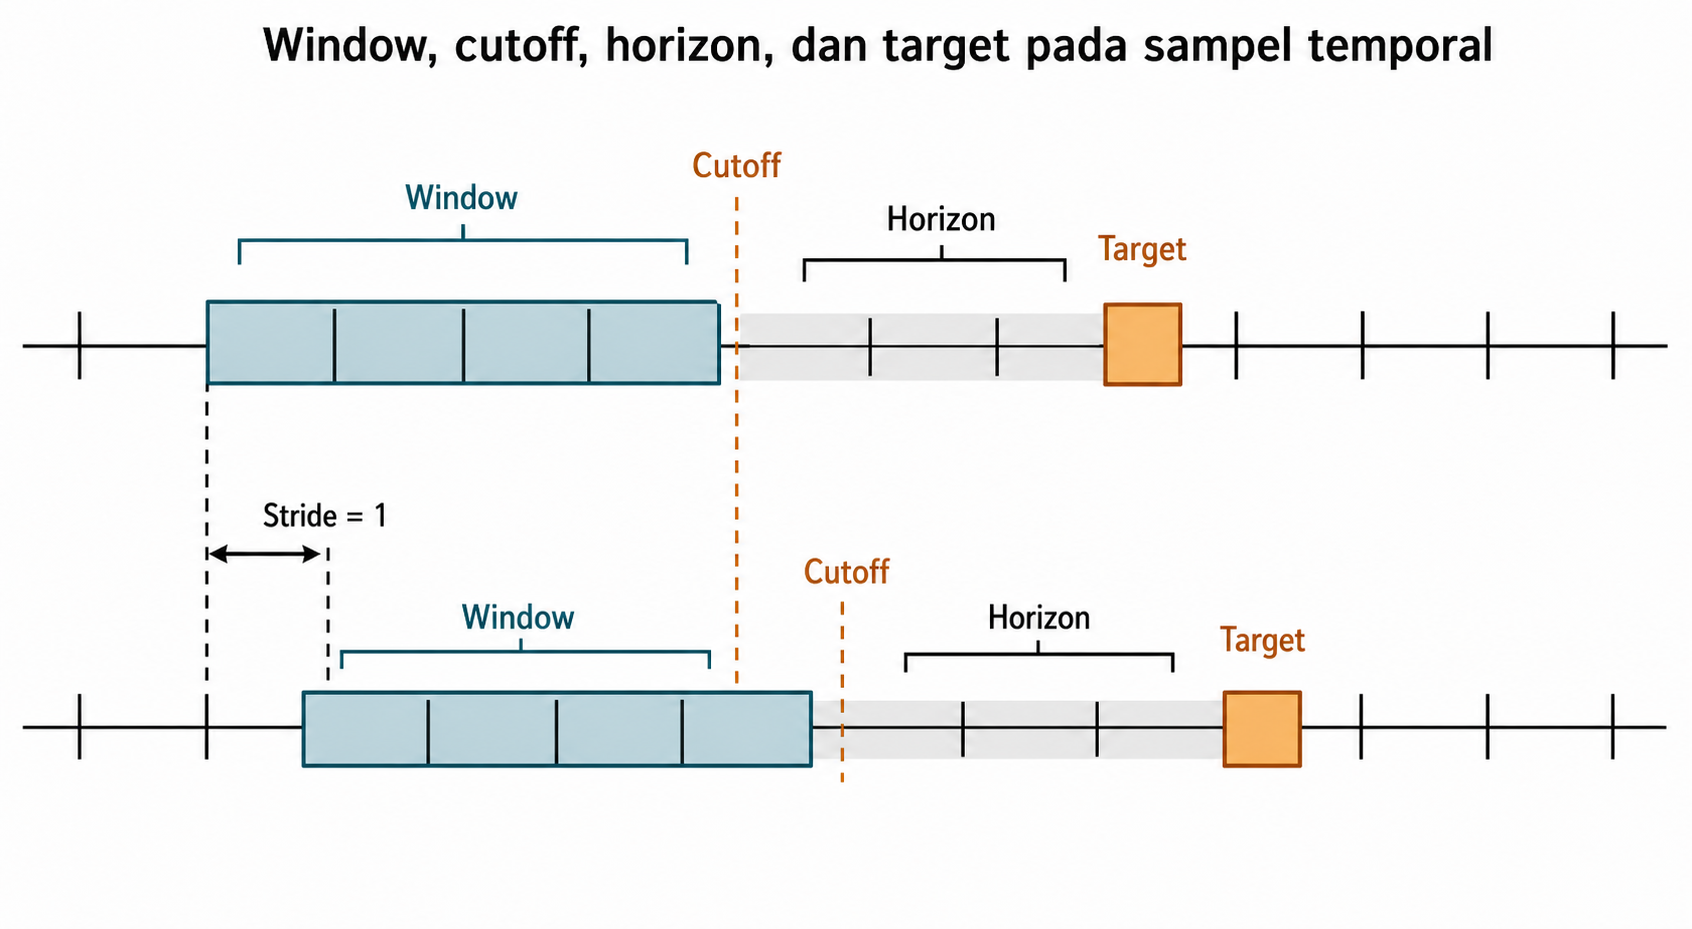
\includegraphics[width=\linewidth,height=0.72\textheight,keepaspectratio]{ch10-fig-1}
\caption{Jendela Rolling dan Expanding pada Deret Waktu}
\label{fig:ch10-fig-1}
\end{figure}

Penyelarasan waktu antara fitur historis dan target masa depan sangat rentan memicu \emph{data leakage}. Praktik \emph{pipeline} yang benar mengharuskan perancangan jendela waktu secara terstruktur. Pendekatan pertama, \emph{causal window}, menempatkan batas akhir jendela input tepat sebelum awal \emph{horizon}. Metode ini memastikan model hanya memproses data historis untuk memprediksi masa depan, menjadikannya syarat mutlak untuk tugas \emph{forecasting}. Pendekatan kedua, \emph{centered window}, merangkum observasi sebelum dan sesudah suatu titik waktu. Penggunaan skema ini pada kasus \emph{forecasting} akan mendistorsi model karena informasi masa depan masuk sebagai input. Oleh karenanya, \emph{centered window} dibatasi hanya untuk analisis retrospektif, seperti imputasi nilai kosong atau penghalusan tren.

Terakhir, pembentukan sampel ini menuntut interval waktu antarpengamatan yang konstan. Praktiknya, data sensor atau log transaksi sering tercatat dengan interval tidak beraturan sehingga wajib diseragamkan (\emph{resampling}) terlebih dahulu. Pengguna dapat menerapkan \emph{downsampling} untuk mengagregasi frekuensi tinggi menjadi interval yang lebih rendah, atau \emph{upsampling} untuk mengestimasi nilai pada celah antarpengamatan. Dengan interval yang konstan, setiap pergeseran \emph{stride} akan memuat rentang historis yang ekuivalen untuk dipelajari oleh algoritma.

\section{\texorpdfstring{Fitur Lag dan Statistik \emph{Rolling}}{Fitur Lag dan Statistik Rolling}}\label{fitur-lag-dan-statistik-rolling}

Setelah mengonstruksi \emph{lookback window}, langkah selanjutnya adalah mengekstraksi rentang waktu tersebut menjadi atribut diskrit. Tujuan utama tahap ini adalah meratakan dimensi waktu. Model \emph{machine learning} tabular standar beroperasi pada baris dan kolom yang saling lepas dan tidak memiliki mekanisme bawaan untuk mengenali urutan kejadian. Dengan memetakan riwayat pengamatan menjadi kolom-kolom baru, kita mengonversi proses historis yang dinamis menjadi deretan prediktor statis.

Cara paling langsung untuk merepresentasikan masa lalu adalah melalui fitur \emph{lag}. Fitur ini menarik nilai observasi dari langkah waktu sebelumnya untuk digunakan sebagai prediktor pada saat ini. Sebagai contoh, jika kita memprediksi suhu udara hari ini, suhu dari hari kemarin bertindak sebagai fitur \emph{lag} 1, sedangkan suhu dua hari yang lalu menjadi \emph{lag} 2.

Meskipun fitur \emph{lag} efektif menyediakan referensi terdekat, penggunaannya yang berlebihan dapat memunculkan kendala struktural. Ekstraksi riwayat yang terlalu jauh ke belakang secara terpisah akan menambah dimensi matriks \emph{dataset} secara eksponensial. Pelebaran matriks yang diikuti oleh korelasi antarfitur ini menyulitkan model dalam membedakan sinyal prediktif dari \emph{noise}, sehingga probabilitas \emph{overfitting} meningkat.

Sebagai alternatif untuk menangkap pola historis tanpa memperbanyak dimensi kolom, pengguna menerapkan agregasi statistik. Pendekatan pertama adalah menggunakan statistik \emph{rolling}, yang meringkas \emph{lookback window} berukuran konstan menjadi satu metrik agregat. Sebagai contoh, alih-alih mengekstraksi observasi 30 hari sebagai 30 prediktor terpisah, data tersebut dihitung menjadi nilai rata-rata, standar deviasi untuk mendeteksi deviasi fluktuasi, atau nilai puncak observasi. Metrik representatif dalam kelompok ini mencakup \emph{Simple Moving Average}, yang diformulasikan sebagai \(SMA_t = \frac{1}{w} \sum_{i=0}^{w-1} x_{t-i}\). Pada perumusan tersebut, \(SMA_t\) adalah nilai rata-rata bergerak pada waktu \(t\), variabel \(w\) menentukan ukuran jendela, dan \(x_{t-i}\) adalah nilai aktual pada \(i\) langkah sebelum \(t\). Penentuan ukuran jendela ini membutuhkan keseimbangan fungsional; jendela yang sempit merekam dinamika terkini namun sangat terpengaruh oleh \emph{noise}, sedangkan jendela yang panjang menyediakan stabilitas pembacaan tren namun lambat dalam merefleksikan perubahan arah musiman.

Pendekatan kedua adalah menggunakan statistik \emph{expanding}. Berbeda dengan pergeseran interval pada metode \emph{rolling}, \emph{expanding window} menahan titik awal pengamatan pada batas tetap, sedangkan ujung observasi berlanjut sejalan masuknya baris \emph{dataset} baru. Mekanisme ini diaplikasikan untuk membangun rekam jejak kumulatif masa lalu, seperti metrik total volume transaksi sistem sejak fase aktivasi awal hingga waktu observasi terkini.

\begin{figure}[htbp]\centering
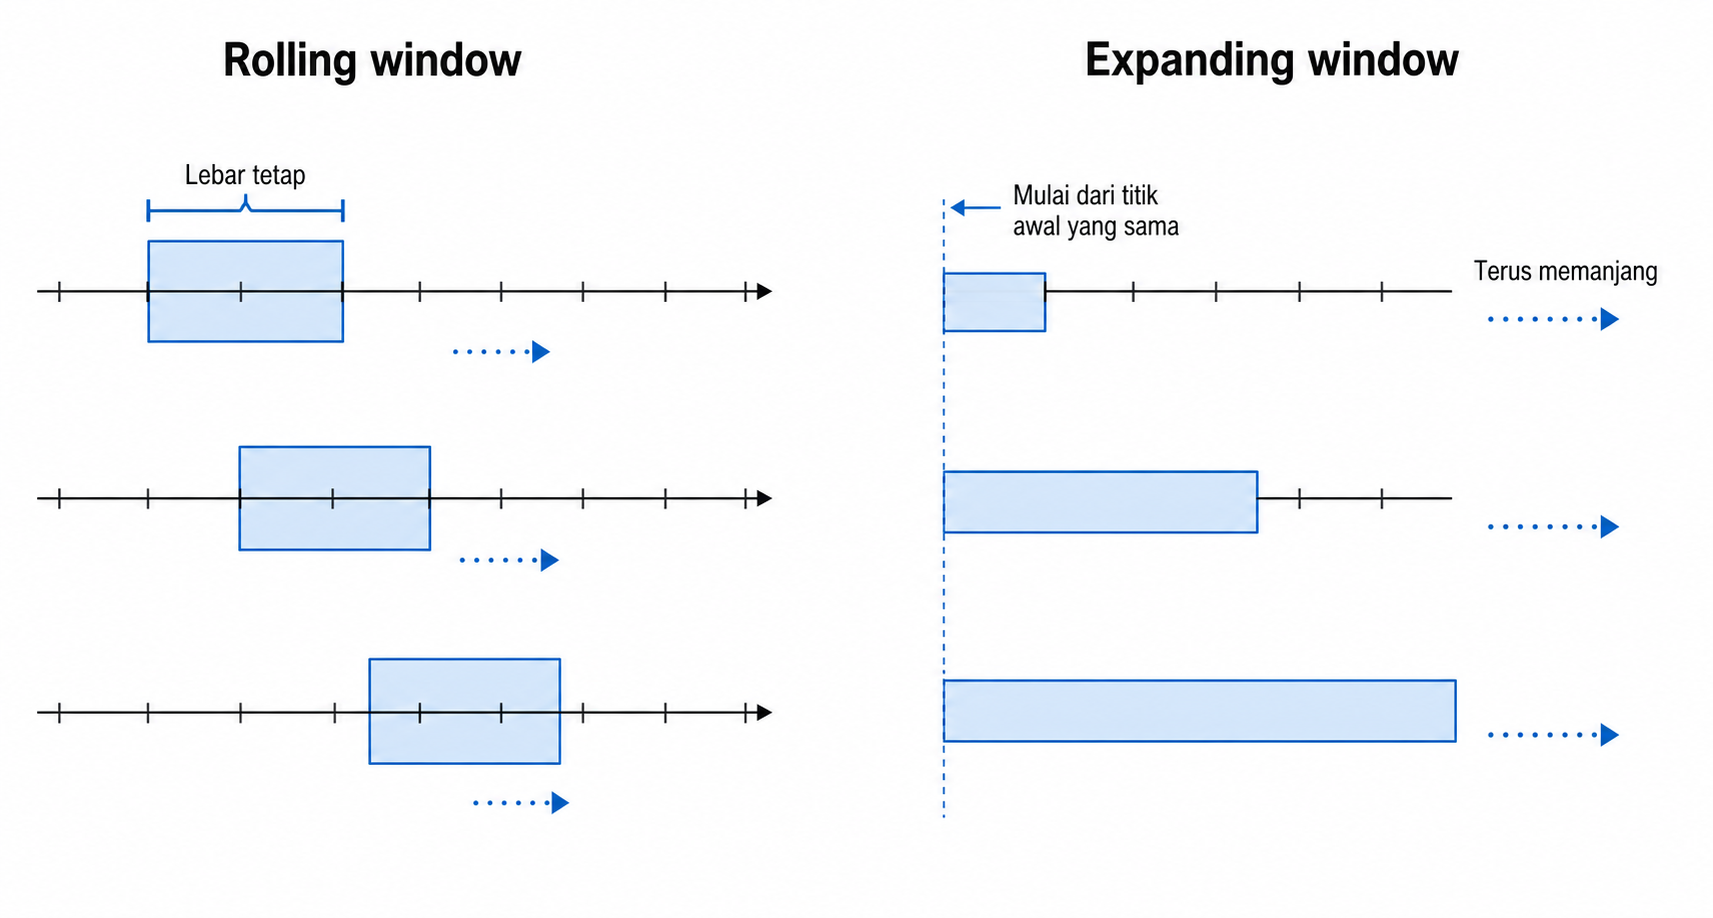
\includegraphics[width=\linewidth,height=0.72\textheight,keepaspectratio]{ch10-fig-2}
\caption{Perbandingan Mekanisme Jendela Bergeser (Rolling) vs Melebar (Expanding)}
\label{fig:ch10-fig-2}
\end{figure}

Melalui kombinasi tiga teknik representasi tersebut (referensi jarak dekat dari \emph{lag}, deteksi tren lokal dari \emph{rolling}, serta observasi kumulatif dari \emph{expanding}), karakteristik data temporal dipetakan secara terstruktur ke dalam format tabular. Pada lingkungan operasional, pustaka pemrosesan runtun waktu seperti \emph{tsfresh} atau komponen transformasi \emph{aeon} melakukan perhitungan puluhan agregasi statistik ini secara sistematis.

\section{Differencing, Tren, dan Pola Musiman}\label{differencing-tren-dan-pola-musiman}

Data deret waktu memiliki dua pola makro yang membedakannya dari data tabular biasa: tren dan musiman. Tren adalah pergerakan arah jangka panjang, seperti angka penjualan yang terus naik dari tahun ke tahun. Musiman adalah fluktuasi periodik yang berulang secara teratur, misalnya lonjakan pengunjung situs setiap akhir pekan.

Bentuk makro seperti tren memberikan hambatan komputasi bagi algoritma, khususnya pada kelompok model berbasis pohon keputusan seperti \emph{random forest} atau \emph{gradient boosting}. Arsitektur klasifikasi ini mempartisi distribusi fitur berdasarkan rentang observasi pelatihan tanpa kemampuan ekstrapolasi. Jika data operasional di lapangan mencapai nilai yang melampaui batas maksimum dari data pelatihan, model tersebut tidak mampu memprediksi titik puncak baru tersebut meskipun observasi secara proporsional memperlihatkan lintasan tren yang meningkat.

Untuk menengahi keterbatasan ekstrapolasi ini, representasi data perlu dikonversi mencapai ekuilibrium stasioner. Stasioneritas merupakan kondisi kestabilan statistik di mana metrik seperti rata-rata dan varians tidak lagi mengalami pergeseran seiring berjalannya waktu. Mekanisme utama untuk membentuk status stasioner adalah transformasi \emph{differencing}. Pendekatan ini mengubah fokus algoritma dari memprediksi nilai akumulatif menjadi memprediksi jarak diferensiasi antar titik waktu konsekutif.

\begin{figure}[htbp]\centering
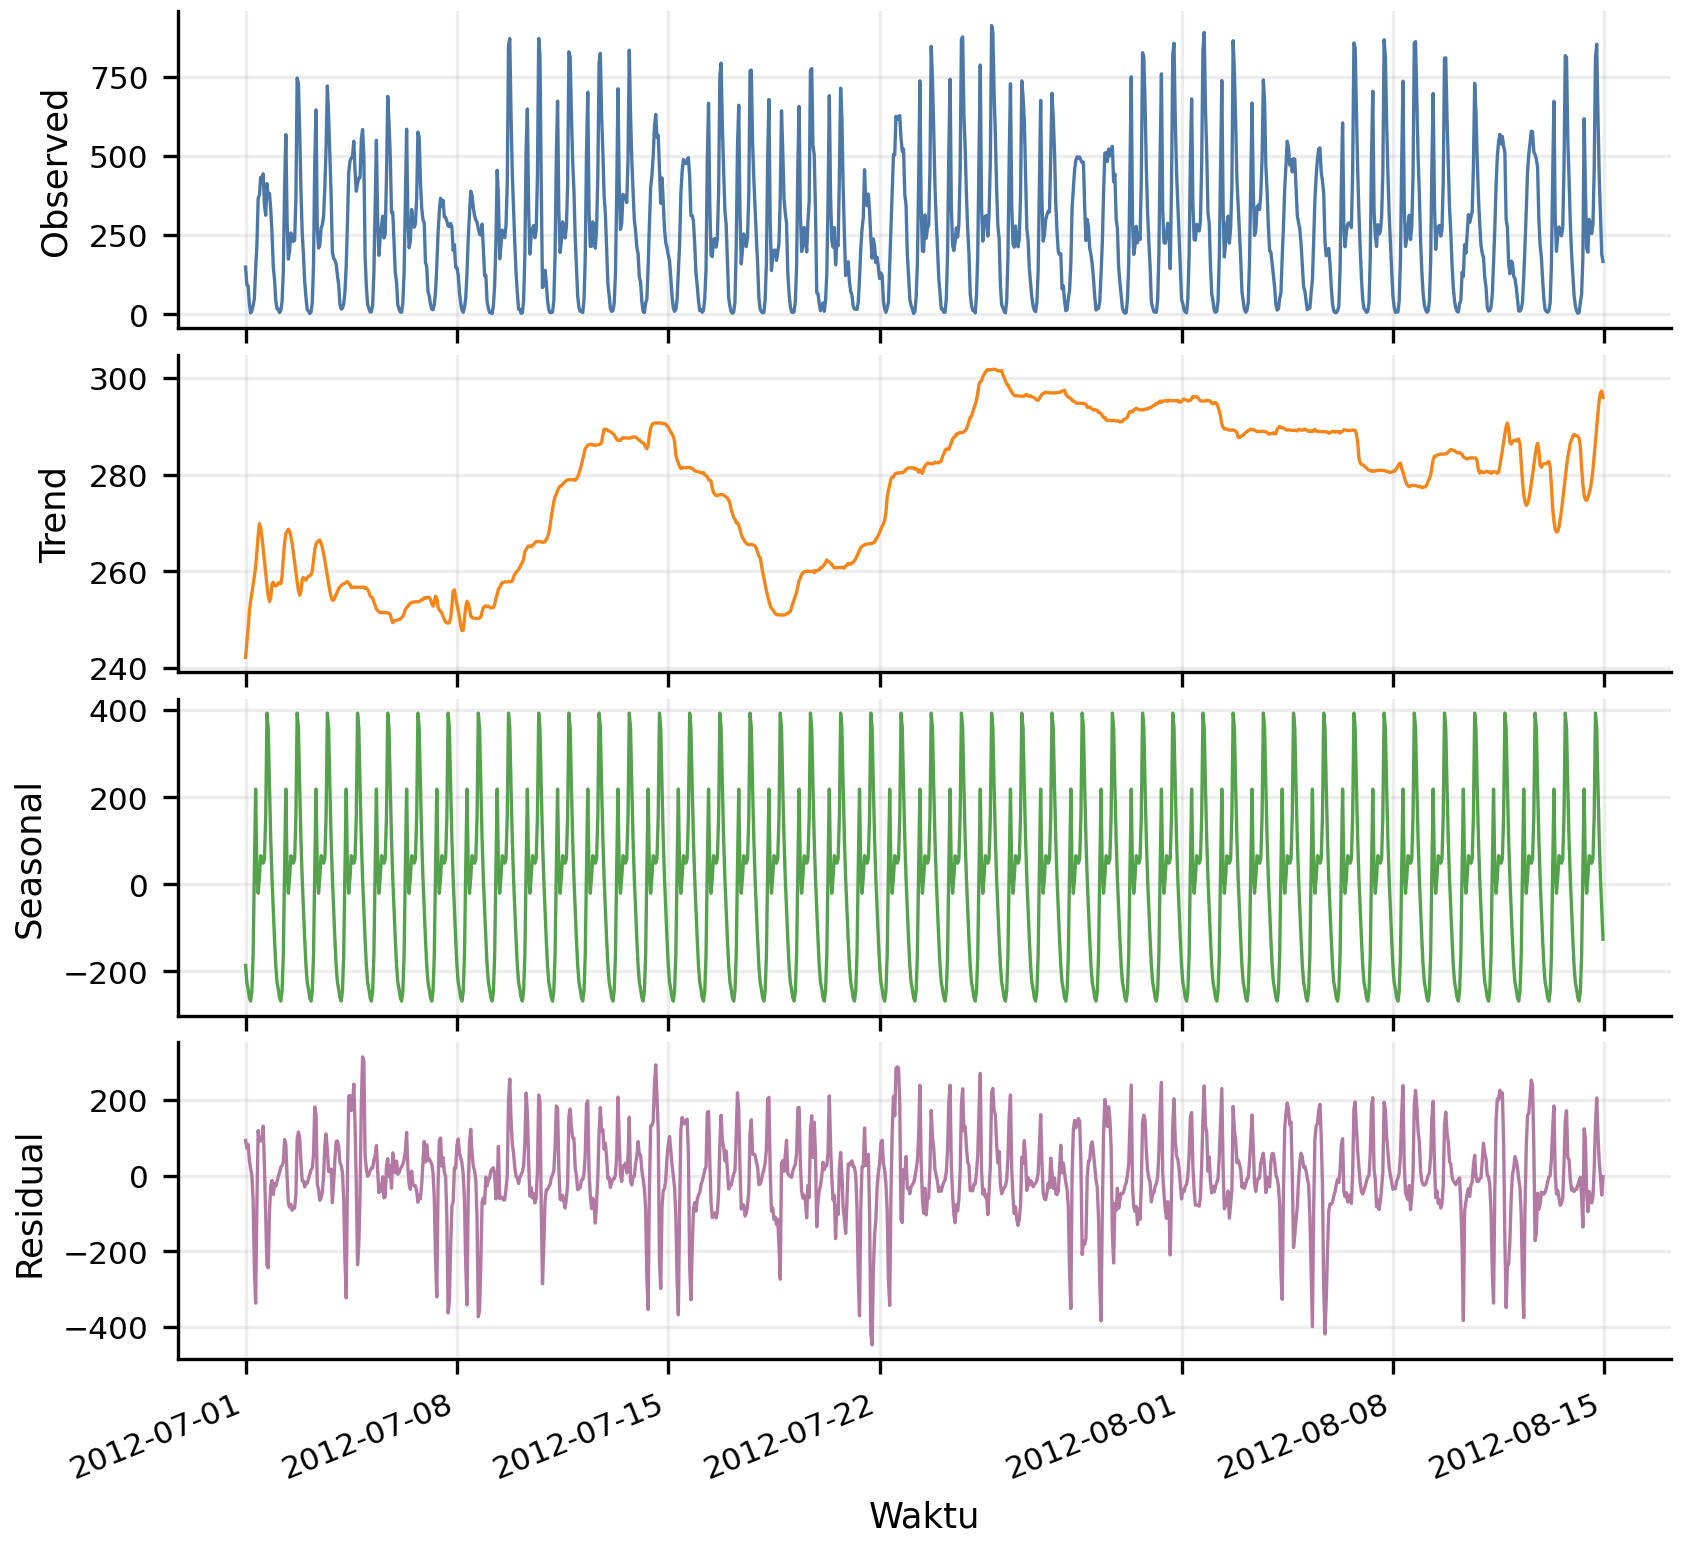
\includegraphics[width=\linewidth,height=0.72\textheight,keepaspectratio]{ch10-fig-3}
\caption{Ekstraksi Fitur Menggunakan tsfresh yang Meratakan Jendela Deret Waktu ke Tabular}
\label{fig:ch10-fig-3}
\end{figure}

Secara matematis, proses \emph{differencing} orde pertama dikalkulasikan melalui rumusan \(y'_t = y_t - y_{t-1}\). Dalam persamaan tersebut, \(y'_t\) merujuk pada nilai luaran hasil transformasi pada langkah waktu \(t\). Adapun \(y_t\) merepresentasikan matriks observasi sebelum modifikasi, dan \(y_{t-1}\) merupakan variabel kondisi observasi dari posisi satu waktu sebelumnya. 

Praktik rekayasa fitur menyediakan ragam modifikasi lain dalam menangani tren maupun periodisitas. Proses \emph{seasonal differencing} digunakan untuk mereduksi efek repetisi dengan menghitung diferensiasi nilai posisi terbaru dengan lokasi ekuivalen pada rotasi sebelumnya, yaitu \(y'_t = y_t - y_{t-m}\), tempat parameter \(m\) membatasi durasi jarak antarpola (misalnya panjang \(m=7\) untuk aktivitas mingguan). Teknik dekomposisi deret waktu juga dapat dieksekusi melalui prosedur analitis STL (\emph{Seasonal and Trend decomposition using Loess}) untuk menyaring sinyal observasi menjadi fraksi tren, sisaan residu, dan efek musim; lalu melatih prediksi model terfokus hanya pada sisaan komponen stasioner residu. Alternatif transformasi lainnya berfokus untuk mencatat pergerakan melalui ekstraksi kemiringan sudut (\emph{slope regression}) dalam blok waktu, maupun penambahan kolom fitur elemen kalender (indikator kategorikal waktu). Penambahan label musim ini mendampingi analisis pola sehingga parameter tren orisinal tetap berada pada format asalnya.

\section{Fitur Domain Frekuensi}\label{fitur-domain-frekuensi}

Seluruh teknik ekstraksi yang memproses urutan nilai berdasarkan waktu, seperti \emph{lag}, \emph{differencing}, maupun statistik \emph{rolling}, beroperasi di dalam domain waktu. Pendekatan ini mengekstrak pola observasi melalui analisis perubahan amplitudo secara berurutan. Format \emph{feature} berbasis waktu tersebut sangat efektif dalam memodelkan set data berfrekuensi rendah, contohnya perubahan agregat penjualan harian atau indikator fluktuasi ekonomi bulanan, di mana transisi absolut pada titik parameter terlihat konstan.

Namun, keterbatasan parameter domain waktu mulai terlihat saat mengelola sinyal data sensor berfrekuensi tinggi. Rangkaian variabel fisik berosilasi rapat, seperti transmisi akselerometer di gawai, sensor getaran di peralatan manufaktur, ataupun pembacaan elektrokardiogram (ECG), mencatat ribuan pengukuran dalam waktu yang sangat singkat. Pada tingkat frekuensi ini, observasi pergeseran simpangan secara berurutan per milidetik jarang merepresentasikan sinyal prediktif yang solid. Pola karakteristik pembentuknya lebih dominan berada pada rasio perulangan gelombang. Untuk mengakomodasi dinamika struktur periodik ini, fokus ekstraksi harus digeser menuju domain frekuensi.

Transisi analitis tersebut dieksekusi secara primer menggunakan metode matematis transformasi Fourier, khususnya algoritma operasional \emph{Fast Fourier Transform} (FFT). Secara fungsi konseptual, perhitungan FFT memisahkan jendela sinyal gabungan ke dalam struktur turunan dari beberapa gelombang komponen sederhana, di mana setiap pecahan gelombang dikategorikan berdasarkan rasio perulangan dan amplitudonya.

\begin{figure}[htbp]\centering

\includegraphics[width=\linewidth,height=0.72\textheight,keepaspectratio]{ch10-fig-4}
\caption{Skema Purge Gap dalam Pemisahan Data Temporal}
\label{fig:ch10-fig-4}
\end{figure}

Penerapan transformasi konseptual ini mendefinisi ulang arsitektur \emph{feature}. Menggantikan pencatatan amplitudo sinyal pada sumbu linier, observasi dikonversi menjadi perhitungan spektrum frekuensi utama (contohnya keberadaan dominan gelombang 50 Hz) dalam keseluruhan batas parameter jendela. Transposisi kerangka waktu menjadi distribusi frekuensi diformulasikan secara teknis menggunakan \emph{Discrete Fourier Transform} (DFT), yang memiliki persamaan dasar \(X_k = \sum_{n=0}^{N-1} x_n \cdot e^{-i 2 \pi k n / N}\). Dalam persamaan tersebut, \(X_k\) adalah komponen spektrum kompleks untuk frekuensi ke-\(k\) yang memuat informasi amplitudo dan fase. Adapun \(x_n\) adalah nilai observasi pada titik waktu ke-\(n\), dan \(N\) adalah jumlah total observasi dalam satu blok perhitungan. Faktor eksponensial \(e^{-i 2 \pi k n / N}\) berperan sebagai gelombang acuan yang mengukur seberapa kuat frekuensi \(k\) hadir dalam sinyal.

Dalam praktiknya, keluaran mentah FFT jarang langsung dipakai untuk pemodelan tabular. Yang diekstrak justru beberapa ringkasan dari spektrum. Puncak frekuensi (\emph{peak frequency}) menandai frekuensi dengan amplitudo terkuat. \emph{Band energy} mengukur total daya pada rentang frekuensi tertentu, sedangkan \emph{spectral centroid} menunjukkan pusat massa sebaran daya di sepanjang spektrum. Entropi spektral melengkapi ukuran ini: nilai yang tinggi menandakan sinyal menyebar seperti \emph{noise}, sedangkan nilai yang rendah menandakan daya terpusat pada sedikit frekuensi.

Dalam \emph{pipeline} rekayasa fitur modern, pengguna tidak perlu membangun algoritma komputasi spektral secara mandiri karena ekosistem pustaka \emph{machine learning} telah menyediakan kerangka kerja fungsional. Modul pemrosesan seperti \passthrough{\lstinline!tsfresh!} dirancang untuk menghitung puluhan variabel frekuensi, mencakup metrik koefisien FFT, kerapatan spektral Welch, hingga entropi komputasi Fourier pada rentang jendela \emph{rolling}. Melengkapi instrumen otomatisasi tersebut, sistem spesifik \emph{pipeline} seperti \passthrough{\lstinline!aeon!} mengintegrasikan fungsionalitas \emph{transformer} data seperti \passthrough{\lstinline!PeriodogramTransformer!} maupun \passthrough{\lstinline!DWTTransformer!} yang memodifikasi komponen operasional \emph{wavelet} ke dalam rancangan prediksi yang bebas dari \emph{data leakage}.

Salah satu aplikasi terstruktur dari representasi frekuensi adalah pada infrastruktur pemeliharaan prediktif (\emph{predictive maintenance}) sistem manufaktur mekanik. Kerusakan awal pada komponen bantalan poros mesin (\emph{bearing}) jarang terdeteksi lewat volume getaran keseluruhan; kondisi aus tersebut justru terekam pada pergeseran parameter fluktuatif serta kenaikan daya spektrum di level tinggi secara sangat terlokalisasi. Ekstraksi spesifik \emph{feature} dari domain spektral inilah yang membuat fungsi pemantauan sanggup mendeteksi deviasi anomali sejak fase awal yang menjadi peringatan dini pencegahan sebelum perangkat memburuk secara fisik. Pembelajaran mengenai mekanisme dekomposisi tersebut turut membangun kerangka teknis analitis gelombang berbasis akustik di Bab 12 yang mengubah aliran suara audio ke dalam matriks gambar dua dimensi berformat spektrogram.

\section{Validasi Temporal: Menghindari Look-Ahead Leakage}\label{validasi-temporal-menghindari-look-ahead-leakage}

Penerapan \emph{cross-validation} acak seperti \emph{K-Fold} pada data deret waktu akan memicu \emph{data leakage}. Pengacakan baris sebelum membagi \emph{dataset} tidak memedulikan susunan kronologis. Sebagai ilustrasi, jika model dilatih menggunakan pengamatan hari Jumat untuk memprediksi target pada hari Kamis, informasi masa depan tersebut sudah diserap oleh fase pelatihan dan validasi. Skema ini menghasilkan evaluasi akurasi semu, di mana performa aktual akan menurun drastis saat algoritma memproses aliran data baru. Pemisahan data untuk kasus temporal wajib mematuhi pemotongan hierarki kronologis (\emph{temporal split}), menempatkan alokasi pelatihan secara eksklusif sebelum rentang blok pengujian. Desain ini menggunakan dua varian; pertama, \emph{expanding window} yang memperbesar ukuran jendela pelatihan namun mempertahankan rentang ukuran uji; dan kedua, \emph{sliding window} di mana blok parameter set data bergeser konstan mengkuti pergerakan kalender operasional.

Meskipun mekanisme \emph{temporal split} menjaga isolasi urutan parameter waktu, formasi observasi berpotensi mengintroduksi bias melalui persinggungan data. Operasional \emph{windowing} menstruktur \emph{dataset} temporal ke dalam barisan parameter yang membentuk \emph{overlapping}. Kondisi ini menyebabkan observasi terakhir di set pelatihan dan \emph{dataset} pertama pada modul validasi bisa saja menggunakan sumber elemen observasi masa lalu yang ekuivalen pada parameter \emph{lookback}. Misalnya pada pemodelan dengan batas \emph{lookback} tujuh hari, baris validasi perdana pada rentang hari ke-100 merekonstruksi rentang matriks mentah dari nilai ke-93 hingga 99; sedangkan komponen data mentah serupa masih masuk ke dalam bagian ekstraksi pengujian observasi hari ke-99 yang dialokasikan di dalam ranah pelatihan. Garis demarkasi perpotongan antar-\emph{dataset} yang bersinggungan langsung tersebut mengaburkan batas objektivitas evaluasi prediksi.

\begin{figure}[htbp]\centering
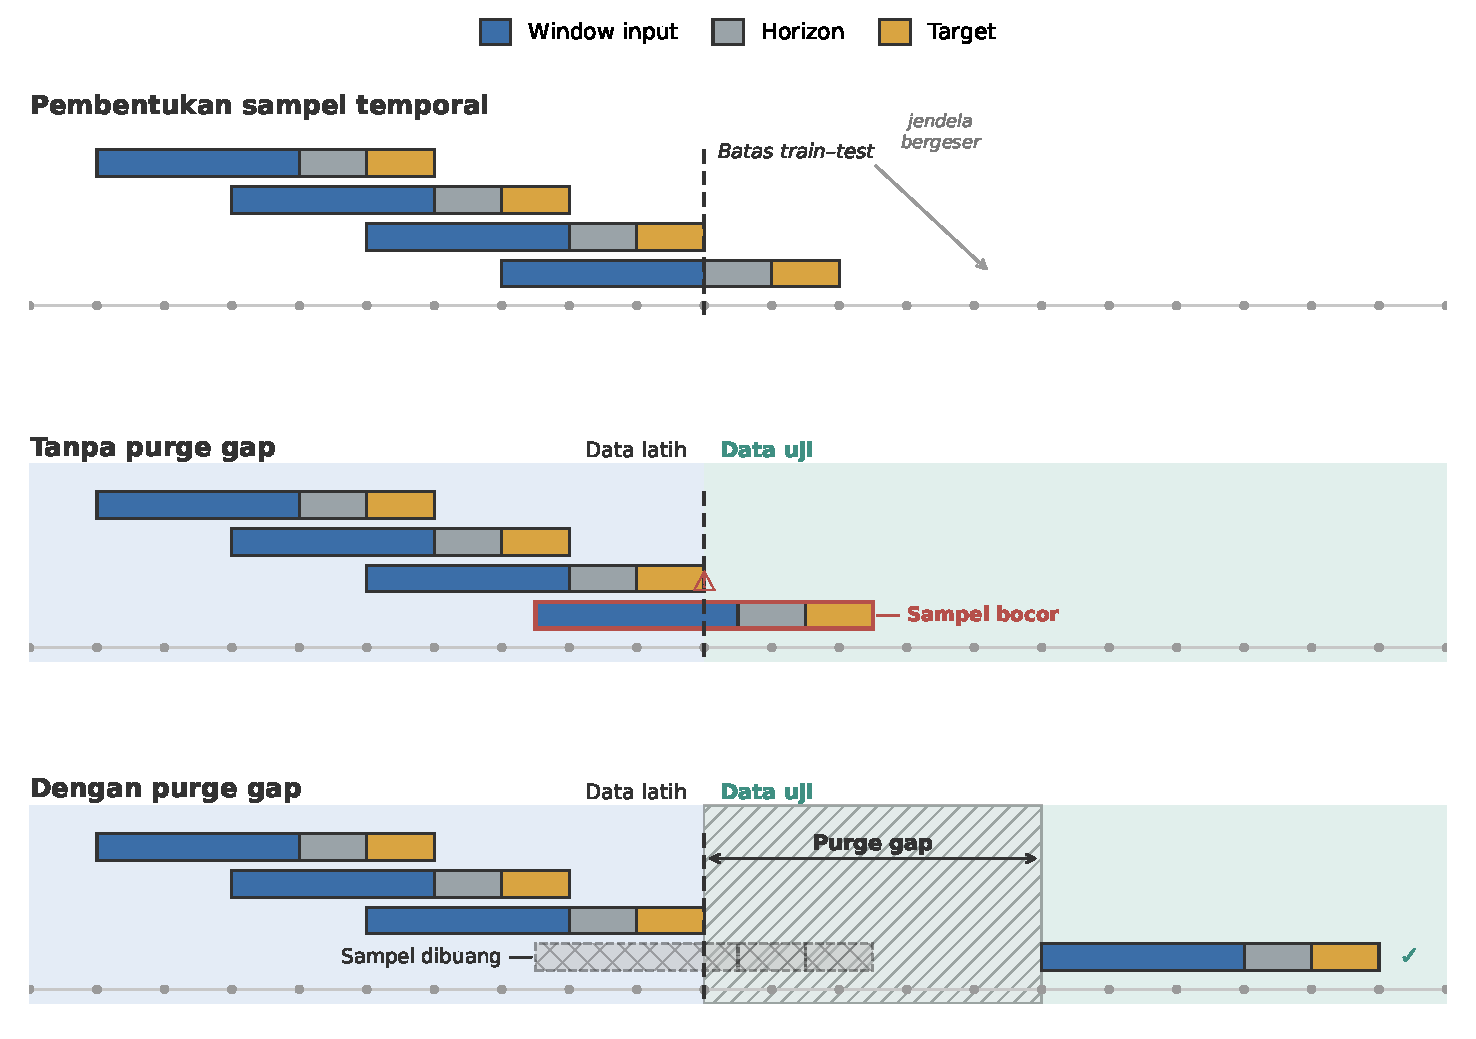
\includegraphics[width=\linewidth,height=0.72\textheight,keepaspectratio]{ch10-fig-5}
\caption{Letak Purge Gap di Antara Set Pelatihan Terakhir dan Set Validasi Pertama}
\label{fig:ch10-fig-5}
\end{figure}

Praktik \emph{pipeline} yang benar mengatasi kerentanan \emph{data leakage} di garis batas pemotongan data dengan cara menyisipkan \emph{purge gap}. Pemisahan \emph{purge gap} bertindak sebagai alokasi observasi perantara yang dieliminasi secara terencana untuk menghindari perpindahan data residu antara parameter batas observasi. Penghitungan panjang observasi yang dibuang diukur melalui parameter eksak \(n_{\text{purge}} = w_{\text{lookback}} + h_{\text{horizon}}\). Formula matematika ini menggunakan variabel \(n_{\text{purge}}\) untuk mewakili ukuran celah data yang dieksklusi, serta \(w_{\text{lookback}}\) sebagai indeks blok langkah historis ke arah belakang. Tambahan variabel \(h_{\text{horizon}}\) mengindikasikan ukuran \emph{horizon} atau unit masa depan prediksi observasi. Parameter prediksi masa depan wajib masuk ke dalam operasi penambahan tersebut karena label target pada rentetan sampel pelatihan ujung merujuk ke elemen data terdepan. Dengan meloncati segmen ini, fungsi pengujian di dalam observasi validasi memperoleh status keterpisahan mutlak tanpa anomali duplikasi elemen data. Dalam sistem \emph{machine learning} saat ini, kerangka fungsional pemrosesan prediksi seperti \passthrough{\lstinline!sktime!} mengoperasikan parameter internal untuk secara spesifik membuang area persinggungan data dari prosedur \emph{cross-validation}. Inisialisasi ruang kosong ini menjamin data \emph{holdout} di fase validasi memperoleh ketahanan evaluasi prediksi.

\section{Fitur untuk Model Klasik vs.~Input Sekuensial}\label{fitur-untuk-model-klasik-vs.-input-sekuensial}

Bentuk rekayasa fitur temporal bergantung pada jenis model yang akan mengolahnya. Model berbasis pohon seperti \emph{random forest} atau \emph{gradient boosting} menerima input sebagai vektor satu dimensi, sehingga urutan waktu harus diratakan lebih dahulu menjadi kolom-kolom terpisah. Model semacam ini tidak menyimpan informasi urutan: setiap fitur dievaluasi sendiri-sendiri tanpa mengetahui posisinya dalam waktu. Karena itu, dimensi waktu perlu dikodekan secara eksplisit melalui fitur turunan seperti \emph{lag} dan agregasi statistik. Pustaka seperti \passthrough{\lstinline!tsfresh!} mengotomasi langkah ini dengan menghitung ribuan fitur sekaligus, lalu meringkasnya menjadi tabel dua dimensi yang siap dilatih.

\begin{figure}[htbp]\centering
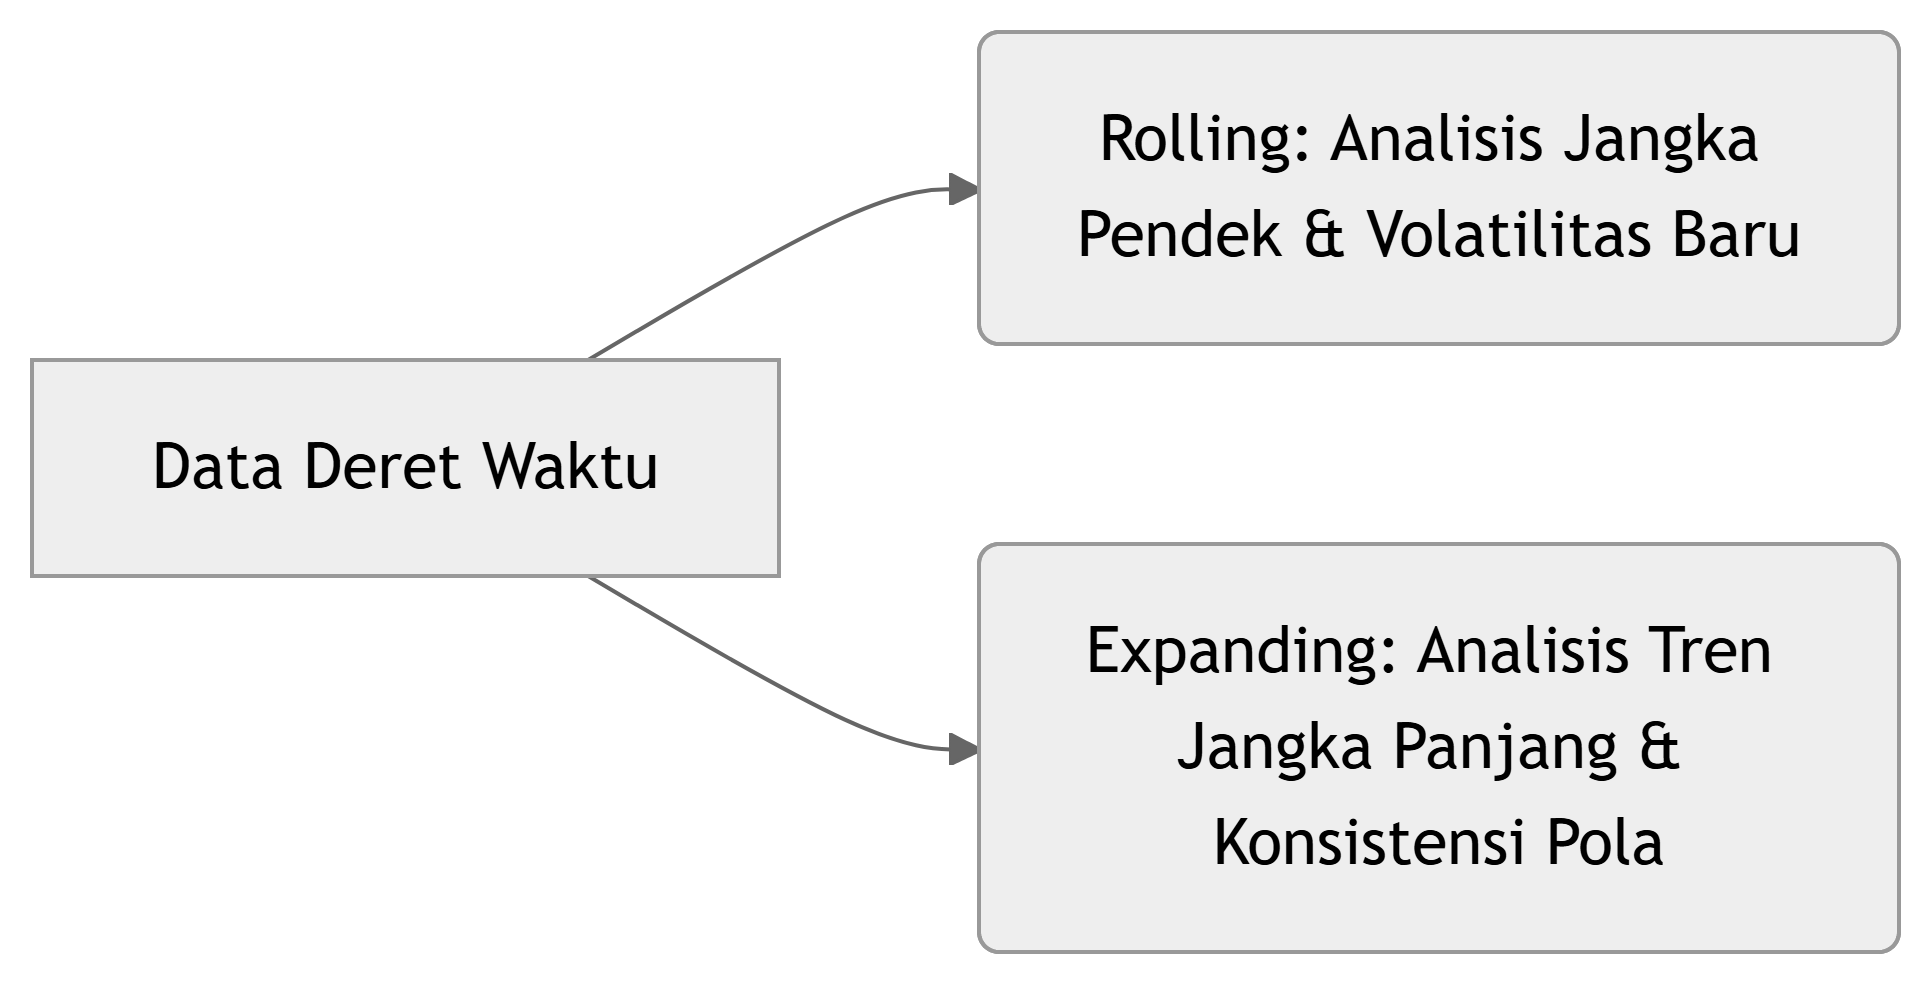
\includegraphics[width=\linewidth,height=0.72\textheight,keepaspectratio]{ch10-fig-6}
\caption{Skema Validasi Temporal dengan Pemisahan Kronologis dan Area Purge Gap}
\label{fig:ch10-fig-6}
\end{figure}

Model sekuensial seperti RNN, LSTM, dan \emph{transformer} bekerja sebaliknya. Fitur tidak diratakan, tetapi dipertahankan sebagai \emph{tensor} dua dimensi dengan satu sumbu langkah waktu dan satu sumbu fitur. Struktur ini menjaga urutan kronologis: model menghubungkan observasi masa lalu dengan masa depan lewat mekanisme internalnya, yaitu \emph{hidden state} pada RNN atau \emph{attention} pada \emph{transformer}. Dengan begitu, ekstraksi pola temporal tidak lagi dirancang manual, melainkan dipelajari sendiri sebagai bobot model selama \emph{training}.

Meski jaringan saraf mampu mengenali urutan observasi, data mentahnya tetap perlu disiapkan, terutama diskalakan agar \emph{gradient} stabil selama \emph{training}. Model ini juga masih memerlukan \emph{cyclical encoding} untuk merepresentasikan waktu yang berulang. \emph{Encoding} tersebut memetakan waktu ke lingkaran melalui fungsi sinus dan kosinus, \(x_{sin} = \sin\left(\frac{2\pi t}{P}\right)\) dan \(x_{cos} = \cos\left(\frac{2\pi t}{P}\right)\), dengan \(t\) sebagai posisi waktu dan \(P\) sebagai panjang satu siklus penuh, misalnya 24 untuk jam dalam sehari. Tanpa \emph{encoding} ini, model menganggap jam 23 dan jam 0 berjauhan, padahal keduanya berdampingan.

Pendekatan modern mulai menggabungkan kedua gaya ini. Lag-Llama, misalnya, memadukan fitur \emph{lag} dengan input mentah dalam satu model. PatchTST memecah deret waktu menjadi potongan-potongan (\emph{patch}) pendek sebelum diproses, sehingga korelasi antarsegmen lebih mudah ditangkap. Ada pula model \emph{foundation} khusus deret waktu seperti \emph{Chronos} dan MOMENT yang dipakai sebagai \emph{feature extractor}: model beku ini mengubah deret mentah menjadi vektor \emph{embedding} padat, yang kemudian diumpankan ke model klasik pada tahap berikutnya.

\section{Studi Kasus: Prediksi Deret Waktu Multivariat}\label{studi-kasus-prediksi-deret-waktu-multivariat}

Studi kasus ini menerapkan rekayasa fitur deret waktu multivariat untuk memprediksi beban listrik suatu wilayah pada langkah waktu berikutnya. Beban listrik dipengaruhi banyak faktor sekaligus, sehingga suhu harian, kelembapan lokal, dan volume konsumsi dicatat sebagai fitur masukan model multivariat. Sebagai \emph{baseline}, kita gunakan \emph{random forest}. Karena model ini menerima input tabular, deret waktu harus diratakan lebih dahulu menjadi baris-baris tunggal. Kita tetapkan \emph{horizon} sepanjang satu langkah ke depan sebagai target, dan \emph{lookback} sepanjang 24 langkah agar setiap sampel merangkum pola beban satu siklus harian sebelumnya.

Dari jendela waktu itu, kita bentuk beberapa kelompok fitur. Pertama, jam (0--23) dikodekan sebagai \emph{cyclical features} dengan sinus dan kosinus, agar model tidak menganggap jam 0 dan jam 23 berjauhan padahal berdampingan. Kedua, 24 fitur \emph{lag} beban listrik menyalin nilai satu hingga 24 jam sebelumnya untuk menangkap pola harian. Ketiga, fitur \emph{rolling} meringkas tren jangka pendek, misalnya rata-rata bergerak suhu, \(MA_t = \frac{1}{w} \sum_{i=0}^{w-1} x_{t-i}\), dengan ukuran jendela \(w=24\) yang merata-ratakan suhu 24 jam terakhir dari titik prediksi.

Tahap selanjutnya adalah perancangan validasi evaluasi prediksi. Proses pengocokan \emph{dataset} baris matriks sangat tidak disarankan karena modifikasi ini mendistorsi kerangka hierarki sekuensial yang menyebabkan masalah \emph{data leakage}. Sebagai pengganti, prosedur evaluasi dijalankan berbekal \emph{temporal split} eksklusif, contohnya memisahkan blok observasi kronologis berupa penggunaan matriks pengamatan murni sepuluh bulan awal dan merelokasi sisa parameter \emph{dataset} berikutnya ke kelompok parameter fungsi pengujian akhir.

Meski pemisahan sudah kronologis, sampel uji pertama tetap membawa 24 fitur \emph{lag} yang nilainya diambil dari sisi pelatihan, tepat di seberang garis potong. Akibatnya, sampel pelatihan terakhir dan sampel uji pertama berbagi sebagian data mentah yang sama. Untuk menghapus irisan ini, kita sisipkan \emph{purge gap} di antara keduanya.

\begin{lstlisting}[language=Python]
import pandas as pd
import numpy as np

# 1. Menyiapkan data deret waktu sintetis (frekuensi per jam selama 30 hari)
date_range = pd.date_range(start='2026-01-01', periods=24*30, freq='h')
np.random.seed(42)
df = pd.DataFrame({
    'Suhu': np.random.normal(loc=25, scale=5, size=len(date_range)),
    'Beban_Listrik': np.random.normal(loc=150, scale=30, size=len(date_range))
}, index=date_range)

# 2. Menentukan titik potong temporal (misalnya: 80% pelatihan, 20% pengujian)
split_point = df.index[int(len(df) * 0.8)]

# 3. Mendefinisikan ukuran Purge Gap (contoh: 25 jam)
purge_gap_hours = 25
purge_gap_delta = pd.Timedelta(hours=purge_gap_hours)

# 4. Melakukan pemisahan temporal secara ketat dengan menyertakan Purge Gap
X_train = df[:split_point]
# Set pengujian dimulai setelah split_point + purge_gap_delta untuk membuang overlap
X_test = df[split_point + purge_gap_delta:]

# 5. Memverifikasi isolasi temporal
print(f"Batas Terakhir Set Pelatihan: {X_train.index[-1]}")
print(f"Batas Awal Set Pengujian   : {X_test.index[0]}")
print(f"Jarak Waktu Antar Set      : {X_test.index[0] - X_train.index[-1]}")
print(f"Jumlah Baris Terbuang (Gap): {len(df) - (len(X_train) + len(X_test))} jam")
\end{lstlisting}

Kode di atas menjalankan bagian inti dari isolasi temporal, yaitu penyisipan \emph{purge gap}. Celah sepanjang 25 jam dipotong tepat di titik pemisahan; angka ini setara dengan panjang \emph{lookback} ditambah \emph{horizon}, sehingga cukup untuk membuang seluruh irisan data antara set pelatihan dan pengujian. Pada \emph{pipeline} yang lengkap, langkah ini dilanjutkan dengan penskalaan yang di-\emph{fit} hanya pada data pelatihan lalu diterapkan ke data uji, agar statistik masa depan tidak ikut membentuk parameter praproses. Dengan jendela yang dirancang rapi dan \emph{purge gap} yang memisahkan kedua set, metrik yang dihasilkan mencerminkan kemampuan model di data baru sebelum diterapkan pada skala \emph{production}.

% ==========================================================================
% ch11.tex — dihasilkan dari v2/drafts oleh tools/md2tex.py
% Sumber: v2\drafts\ch11\ch11_draft_v2.md
% Boleh disunting manual; menjalankan md2tex.py lagi akan menimpa.
% ==========================================================================
\chapter{Teks dan Dokumen}\label{teks-dan-dokumen}

Teks tidak langsung dapat dipakai oleh kebanyakan model pembelajaran mesin. Model menerima token, karakter, dan pola lokal di sekitar kata, bukan makna yang dipahami pembaca manusia. Representasi teks menentukan apa yang dianggap sebagai token, seberapa banyak urutan kata dipertahankan, dan bagaimana kata langka atau konteks ditangani. Representasi klasik menghasilkan representasi yang dirancang manusia, umumnya dalam bentuk fitur \emph{sparse}. \emph{Embedding} dan model bahasa menghasilkan representasi yang dipelajari mesin, umumnya dalam bentuk vektor padat. Keduanya tetap berguna, bergantung pada data, tugas, biaya, dan kebutuhan interpretasi.

Bab ini membahas tangga representasi teks, dimulai dari tokenisasi dan bag-of-words, kemudian pembobotan TF-IDF, word embedding, contextual embedding, sentence dan document embedding, hingga \emph{pretrained language model} sebagai penghasil fitur. Setiap langkah menambah kemampuan menangkap makna, tetapi juga menambah keputusan tentang vocabulary, konteks, penggabungan (pooling), biaya, reproduktibilitas, dan validasi. Bab ini juga menguraikan perbedaan antara membekukan encoder sebagai penghasil fitur dan memperbarui bobotnya melalui fine-tuning.

\section{Representasi Teks Klasik}\label{representasi-teks-klasik}

Contoh kerja pada bagian ini adalah klasifikasi pesan SMS. Setiap dokumen berupa satu pesan pendek, dan targetnya membedakan spam dari pesan sah atau \emph{ham}. Panjang, ejaan, dan tanda baca tidak seragam. Raw text adalah urutan simbol dengan panjang berbeda. Model tabular klasik membutuhkan vektor numerik berukuran tetap. Langkah pertama adalah tokenization, yaitu memecah teks menjadi unit yang akan dihitung atau diberi representasi. Token dapat berupa kata, subword, karakter, atau \emph{n-gram}.

Word-level tokenization mudah dipahami, tetapi rapuh terhadap kata di luar vocabulary. Kata baru, typo, variasi slang, dan bentuk berimbuhan dapat tidak dikenali. Subword tokenization, seperti Byte-Pair Encoding, memecah kata menjadi potongan yang lebih kecil sehingga kata yang belum pernah muncul tetap dapat dirangkai dari bagian yang dikenal. Jika tokenizer dilatih secara lokal, aturan penggabungannya harus dipelajari hanya di dalam data pelatihan setiap \emph{fold}. Berbeda dari itu, tokenizer yang dikirim bersama encoder \emph{pretrained} adalah artefak tetap: jangan melatih ulang vocabulary atau aturan subword-nya pada korpus proyek, dan gunakan versi yang sama pada pelatihan, validasi, serta inferensi.

Setelah tokenisasi, vectorization mengubah korpus menjadi document-term matrix. Baris adalah dokumen, kolom adalah token atau \emph{n-gram}, dan isi sel adalah hitungan atau bobot. Dalam \emph{bag-of-words}, urutan kata diabaikan. Dokumen \(d\) dapat ditulis sebagai vektor berikut.

\[
\mathbf{v}_d = [x_1, \dots, x_{|V|}]
\]

Dalam vektor ini, \(|V|\) adalah ukuran vocabulary, dan \(x_i\) adalah jumlah kemunculan token ke-\(i\) dalam dokumen \(d\). Sebagian besar entri bernilai nol karena satu dokumen hanya memakai sebagian kecil vocabulary.

Kelemahan utama \emph{bag-of-words} adalah buta urutan. Kalimat ``kucing mengejar tikus'' dan ``tikus mengejar kucing'' memiliki hitungan kata yang sama, padahal maknanya berbeda. \emph{N-gram} menambahkan urutan lokal. Bigram seperti ``tidak bagus'' dapat menangkap negasi yang hilang jika ``tidak'' dan ``bagus'' hanya dihitung terpisah. Namun, \emph{n-gram} membuat dimensi tumbuh cepat.

Gambar 11.1 memperlihatkan alur klasik. Kalimat mentah dipecah menjadi token atau subword, lalu masuk ke matriks sparse yang sebagian besar berisi nol. Jika \emph{n-gram} ditambahkan, vocabulary bertambah dan matriks makin lebar.

\begin{figure}[tbp]\centering
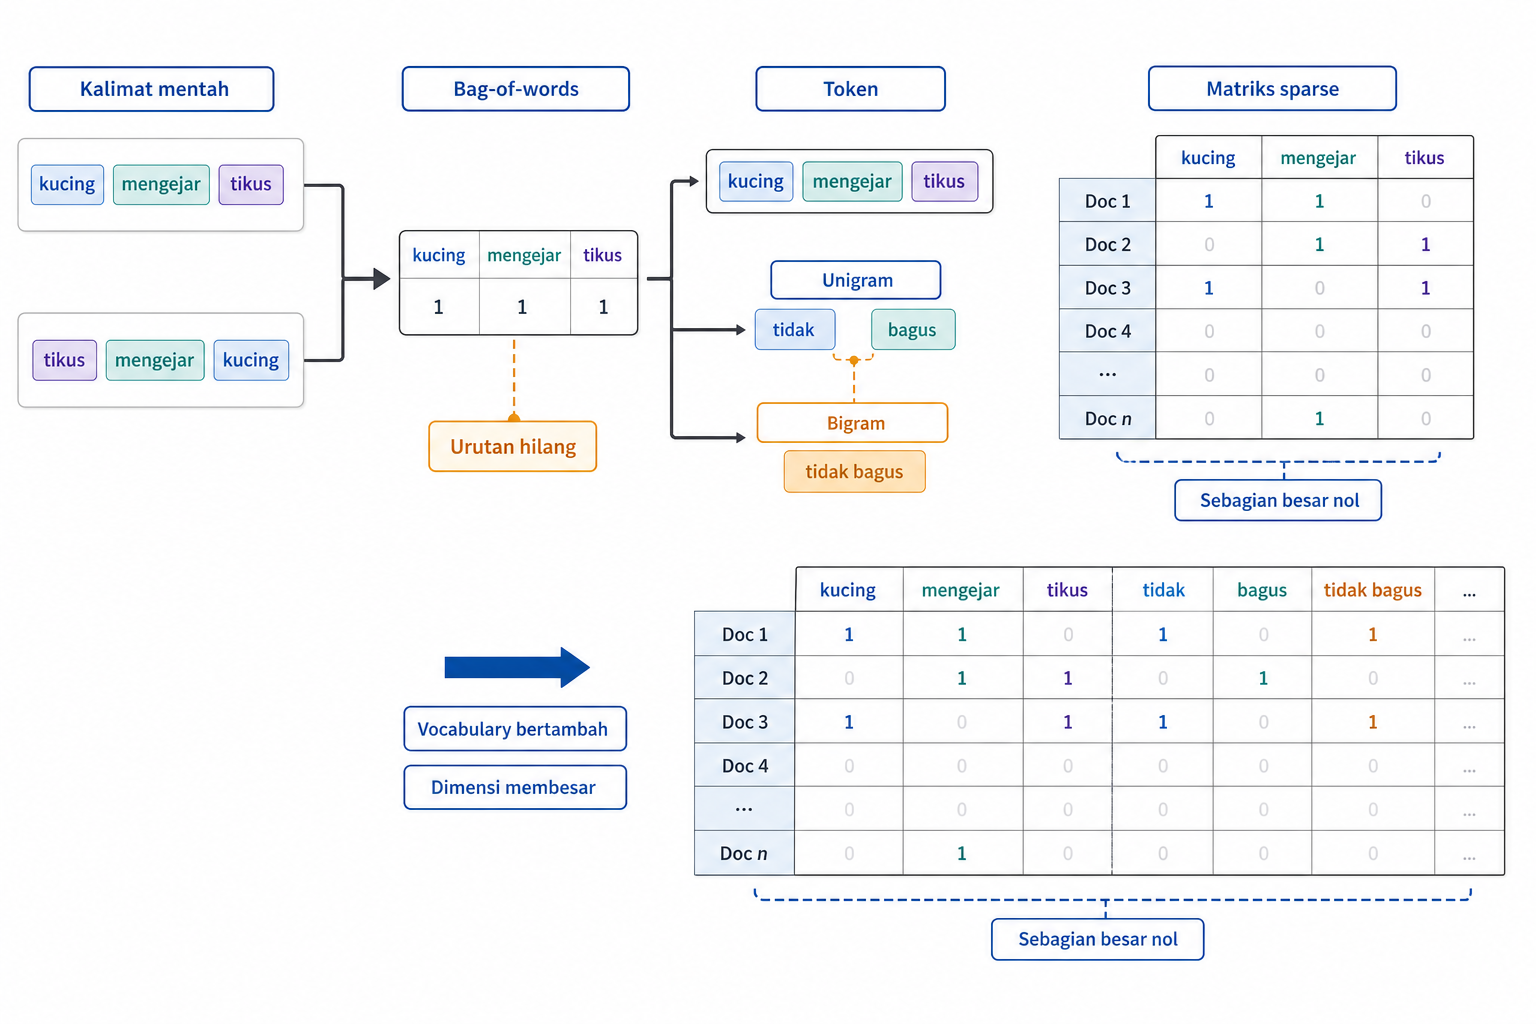
\includegraphics[width=111.6mm]{ch11-fig-1}
\caption{Dari teks mentah ke matriks sparse}
\label{fig:ch11-fig-1}
\end{figure}

Contoh klasiknya adalah deteksi SMS spam. Token seperti ``free'', ``call'', ``txt'', angka nominal, nomor telepon, atau bigram promosi dapat menjadi fitur. Character n-grams sering membantu karena spam dapat memakai variasi ejaan, kapitalisasi, atau tanda baca untuk menonjol tanpa benar-benar mengubah pesan.

Untuk \emph{bag-of-words} atau vectorizer lokal lain, vocabulary harus dipelajari dari data pelatihan, lalu dipakai ulang untuk validasi, test, dan inferensi. Jika vocabulary lokal dibuat dari seluruh korpus sebelum split, token yang hanya muncul di validasi sudah ikut memengaruhi representasi. Aturan ini tidak berarti tokenizer tetap milik model \emph{pretrained} perlu di-\emph{fit} ulang. Untuk produksi dengan vocabulary sangat besar, \passthrough{\lstinline!HashingVectorizer!} dapat memetakan token langsung ke indeks kolom tanpa menyimpan vocabulary, memakai hashing trick yang sama dengan Bab 4 dan membawa risiko collision yang sama. Setelah hitungan token terbentuk, masalah berikutnya adalah pembobotan. Tidak semua kata yang sering muncul sama informatifnya.

\section{\texorpdfstring{\emph{TF-IDF}}{TF-IDF}}\label{tf-idf}

Hitungan mentah sering terlalu memberi bobot pada kata umum. Dalam korpus SMS berbahasa Inggris, kata fungsi seperti ``to'', ``the'', ``and'', atau ``you'' dapat muncul sangat sering, tetapi jarang memberi sinyal spam sendirian. Sebaliknya, token seperti ``free'', ``claim'', ``prize'', nomor pendek, atau pola ``call now'' mungkin muncul lebih jarang, tetapi lebih informatif.

\emph{TF-IDF} (Salton and Buckley 1988) menggabungkan term frequency dan inverse document frequency. Term frequency menyatakan seberapa sering term muncul dalam dokumen.

\[
\text{TF}(t, d) = f_{t,d}
\]

Inverse document frequency memberi bobot lebih rendah pada term yang muncul di banyak dokumen.

\[
\text{IDF}(t) = \log \dfrac{N}{df_t}
\]

Dalam rumus IDF, \(N\) adalah jumlah dokumen, dan \(df_t\) adalah jumlah dokumen yang mengandung term \(t\). Bobot akhirnya diperoleh dengan mengalikan keduanya.

\[
\text{TF-IDF}(t, d) = \text{TF}(t, d) \times \text{IDF}(t)
\]

Implementasi dapat berbeda dalam smoothing dan penskalaan bobot, tetapi idenya sama. Kata yang sering dalam satu dokumen tetapi jarang di seluruh korpus menjadi menonjol.

Kontrasnya sederhana. Kata ``you'' bisa memiliki TF tinggi dalam banyak pesan, tetapi IDF-nya rendah karena muncul hampir di mana-mana. Token seperti ``prize'' atau pola nomor tertentu mungkin hanya muncul pada sedikit pesan sehingga mendapat IDF lebih tinggi. IDF hanya mengukur kelangkaan dokumen dan tidak melihat label spam. Hubungan token dengan kelas dipelajari oleh model terawasi atau metode seleksi terawasi, bukan oleh IDF.

\emph{TF-IDF} masih termasuk representasi yang dirancang manusia dan berbentuk \emph{sparse}. Representasi ini sering menjadi \emph{baseline} kuat untuk klasifikasi dokumen, pencarian, dan dataset kecil sampai menengah. Namun, \emph{TF-IDF} tidak memahami sinonim, konteks, atau urutan kata di luar \emph{n-gram}. ``Mobil'' dan ``kendaraan'' tetap kolom berbeda. Kata yang sama dalam konteks berbeda tetap dihitung sama.

IDF dipelajari dari korpus pelatihan. Jika \emph{TF-IDF} di-\emph{fit} pada seluruh dokumen sebelum validasi, statistik dokumen validasi ikut menentukan bobot. Ini adalah \emph{leakage} representasi. Seperti transformer lain yang belajar statistik lokal, vectorizer harus hidup di dalam pipeline validasi. Sebaliknya, tokenizer tetap yang menyertai encoder \emph{pretrained} dimuat apa adanya dan tidak di-\emph{fit} pada tiap \emph{fold}. Keterbatasan utama \emph{TF-IDF} tetap sama. Kolom sparse tidak tahu bahwa dua kata dapat berdekatan makna. Bagian berikut memperkenalkan representasi padat yang belajar kedekatan itu dari data.

\begin{pendalaman}{Sublinear TF dan BM25}
Sublinear TF mengganti hitungan mentah dengan \(1 + \log(\text{TF})\), sehingga kata yang muncul 100 kali tidak otomatis berbobot 100 kali kemunculan tunggal. Dalam \passthrough{\lstinline!TfidfVectorizer!}, ini terkait opsi \passthrough{\lstinline!sublinear_tf!}. BM25 mengembangkan ide tersebut untuk \emph{retrieval} dengan menambahkan penyesuaian panjang dokumen dan saturasi frekuensi term. BM25 tetap menjadi \emph{baseline} leksikal yang kuat dalam sistem pencarian. Pada \emph{hybrid search}, BM25 menyumbang sisi \emph{sparse} yang melengkapi pencarian semantik.
\end{pendalaman}

\section{\texorpdfstring{Pergeseran ke Representasi yang Dipelajari melalui \emph{Word Embedding}}{Pergeseran ke Representasi yang Dipelajari melalui Word Embedding}}\label{pergeseran-ke-representasi-yang-dipelajari-melalui-word-embedding}

Pada representasi sparse, setiap kata menjadi kolom terpisah. Kata ``mobil'' dan ``kendaraan'' tidak berbagi apa pun kecuali keduanya kebetulan muncul di dokumen yang sama. Model harus belajar hubungan tiap kata dengan target hampir dari nol. Ini tidak efisien, terutama ketika kata jarang atau ketika banyak sinonim muncul.

Word embedding memetakan token ke vektor padat yang dipelajari dari data. Alih-alih ribuan atau jutaan kolom sparse, setiap token memiliki vektor berdimensi ratusan. Prinsip dasarnya berangkat dari distributional hypothesis. Kata yang muncul dalam konteks serupa cenderung memiliki makna serupa. Word2Vec (Mikolov et al. 2013) dan GloVe mengoperasionalkan gagasan ini pada korpus besar.

Kedekatan embedding sering diperiksa dengan cosine similarity.

\[
\text{sim}(\mathbf{a}, \mathbf{b}) = \dfrac{\mathbf{a} \cdot \mathbf{b}}{\lVert\mathbf{a}\rVert\,\lVert\mathbf{b}\rVert}
\]

Dalam rumus tersebut, \(\mathbf{a}\) dan \(\mathbf{b}\) adalah dua vektor embedding. Nilai mendekati 1 berarti arahnya selaras, nilai mendekati -1 berarti arahnya berlawanan, dan nilai mendekati 0 menunjukkan hubungan yang lemah. Cosine similarity menjadi probe geometri untuk embedding kata, kalimat, dan dokumen.

Gambar 11.2 membandingkan ruang sparse dan dense. Pada ruang sparse, ``mobil'', ``kendaraan'', dan ``pisang'' berada pada sumbu terpisah yang saling ortogonal. Pada proyeksi dense, ``mobil'' dan ``kendaraan'' dapat berdekatan karena muncul dalam konteks serupa, sementara ``pisang'' berada lebih jauh.

\begin{figure}[tbp]\centering
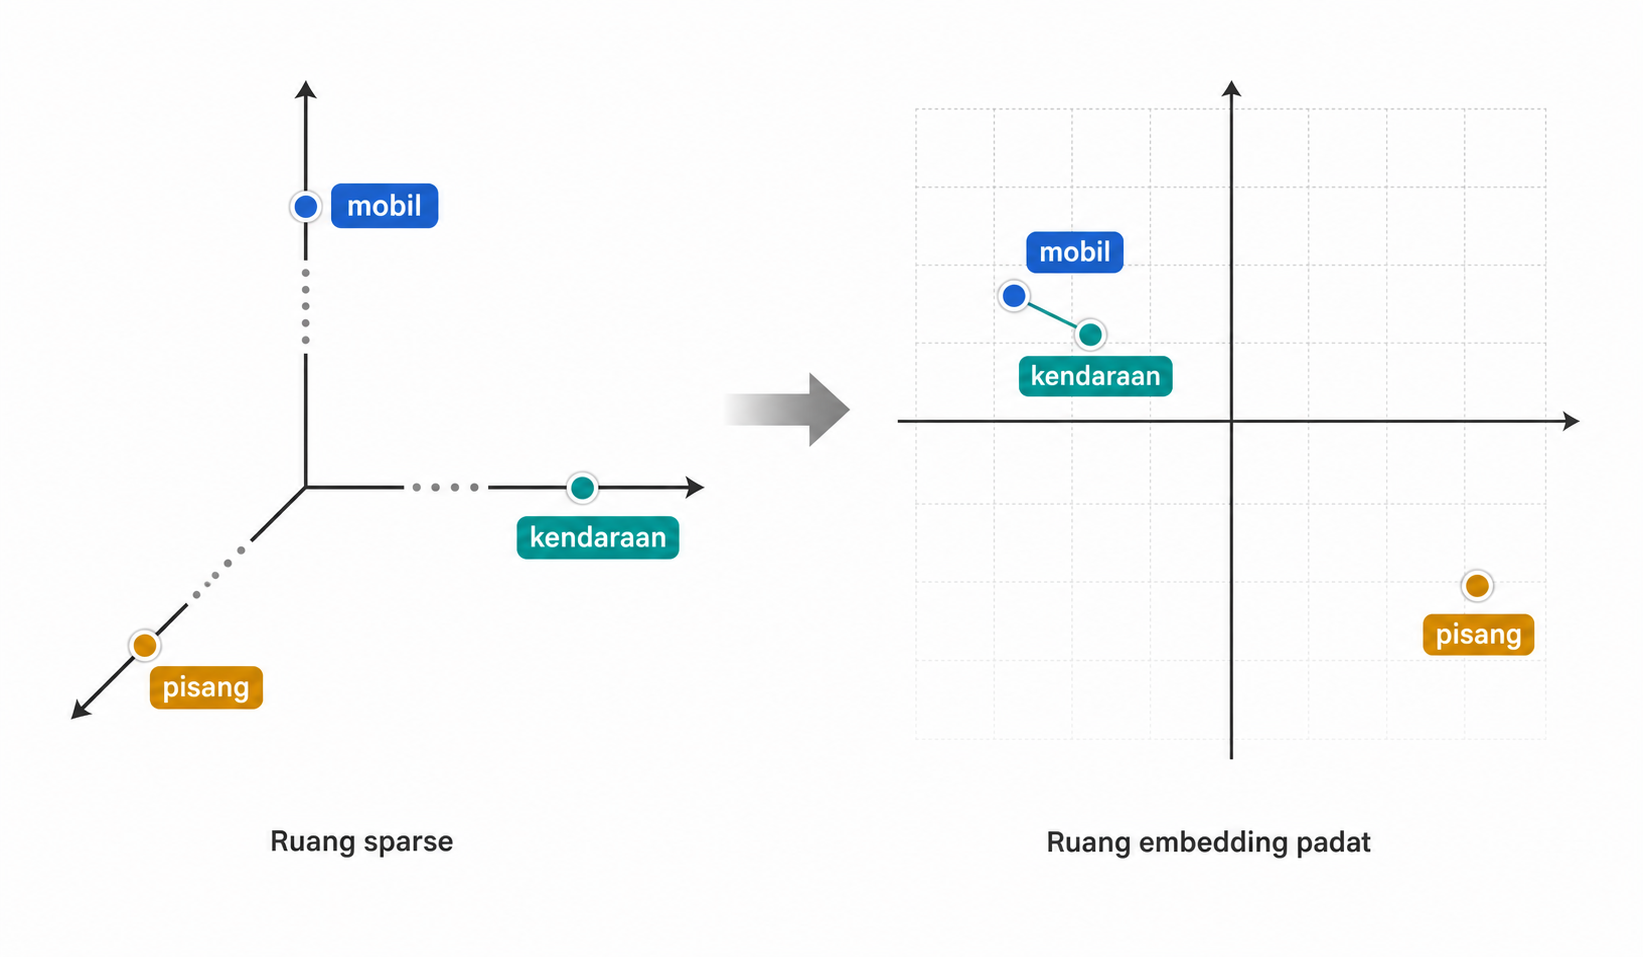
\includegraphics[width=111.6mm]{ch11-fig-2}
\caption{Ruang sparse dan ruang embedding padat}
\label{fig:ch11-fig-2}
\end{figure}

Embedding statis memberi satu vektor untuk satu kata atau token, apa pun konteksnya. Ini memperbaiki masalah sinonim, tetapi belum menyelesaikan polisemi. Kata ``bisa'' sebagai kemampuan dan ``bisa'' sebagai racun tetap berbagi satu vektor jika memakai embedding statis.

Subword atau token-piece embeddings membantu menghadapi kata jarang, morfologi, dan out-of-vocabulary forms. Namun, embedding tetap belajar dari korpus dan tokenizer tertentu. Untuk teks Indonesia yang penuh slang, singkatan, imbuhan, atau code-switching, kecocokan korpus dan tokenizer sangat penting. Embedding bukan berarti model benar-benar ``memahami'' bahasa. Representasi ini mengodekan regularitas statistik dan semantik yang dipelajari dari data. Keterbatasan berikutnya adalah konteks. Satu kata dapat berubah makna bergantung kalimatnya.

\begin{pendalaman}{Subword untuk morfologi, dan embedding Matryoshka}
fastText merepresentasikan kata sebagai jumlah vektor \emph{character n-gram}. Dengan cara ini, bentuk Indonesia yang panjang atau berimbuhan seperti ``dipertanggungjawabkan'' tetap mewarisi informasi dari potongan katanya, sehingga relevan untuk teks informal dan kaya morfologi. Secara terpisah, \emph{Matryoshka representation learning} melatih embedding agar dimensi awal membawa informasi paling penting. Vektor 1024 dimensi dapat dipotong menjadi 256 dimensi saat inferensi dengan penurunan kualitas yang diharapkan tetap terbatas. Pemotongan ini memberi kompromi langsung antara \emph{storage}, \emph{latency}, dan kualitas representasi.
\end{pendalaman}

\section{\texorpdfstring{\emph{Contextual}, \emph{Sentence}, dan \emph{Document Embedding}}{Contextual, Sentence, dan Document Embedding}}\label{contextual-sentence-dan-document-embedding}

Embedding statis memberi satu representasi untuk satu token. Contextual embedding memberi representasi yang bergantung pada kata di sekitarnya. Kata ``bisa'' dalam ``saya bisa datang'' dan ``bisa ular itu berbahaya'' tidak harus mendapat vektor yang sama. Model seperti BERT (Devlin et al. 2019) menghasilkan representasi token atau subword yang berubah sesuai konteks kalimat.

Banyak tugas membutuhkan satu vektor untuk kalimat atau dokumen, bukan vektor per token. \emph{Sentence} dan \emph{document embedding} memampatkan teks menjadi vektor berukuran tetap untuk klasifikasi, \emph{clustering}, \emph{retrieval}, atau \emph{similarity search}. Pilihan \emph{pooling} menjadi penting. \passthrough{\lstinline![CLS]!} adalah salah satu kandidat, tetapi kegunaannya sebagai representasi kalimat bergantung pada cara model dilatih dan diadaptasi. Gunakan mekanisme \emph{pooling} yang didokumentasikan untuk model tersebut; untuk kemiripan semantik, model \emph{sentence embedding} yang memang dilatih dengan objektif kesamaan biasanya lebih tepat daripada mengambil \passthrough{\lstinline![CLS]!} secara otomatis. Pilihan lain mencakup \emph{mean pooling} dan \emph{task-specific pooling}.

Mean pooling naif kadang menghasilkan vektor yang berguna, tetapi operasi ini selalu mengaburkan urutan dan komposisi karena bersifat komutatif terhadap posisi token. Dua kalimat dengan kata serupa tetapi struktur berbeda dapat menjadi terlalu dekat. Itulah sebabnya model seperti Sentence-BERT (Reimers and Gurevych 2019) dilatih khusus agar embedding kalimat memiliki geometri yang lebih cocok untuk similarity dan retrieval.

Gambar 11.3 memperlihatkan alur representasi modern. Dokumen mentah dipecah menjadi token atau subword. Transformer encoder menghasilkan contextual token vectors. Lalu pooling mengubah deretan vektor token menjadi satu vektor kalimat atau dokumen. Langkah pooling ini bukan detail kecil. Pilihan tersebut menentukan informasi apa yang dipertahankan.

\begin{figure}[tbp]\centering
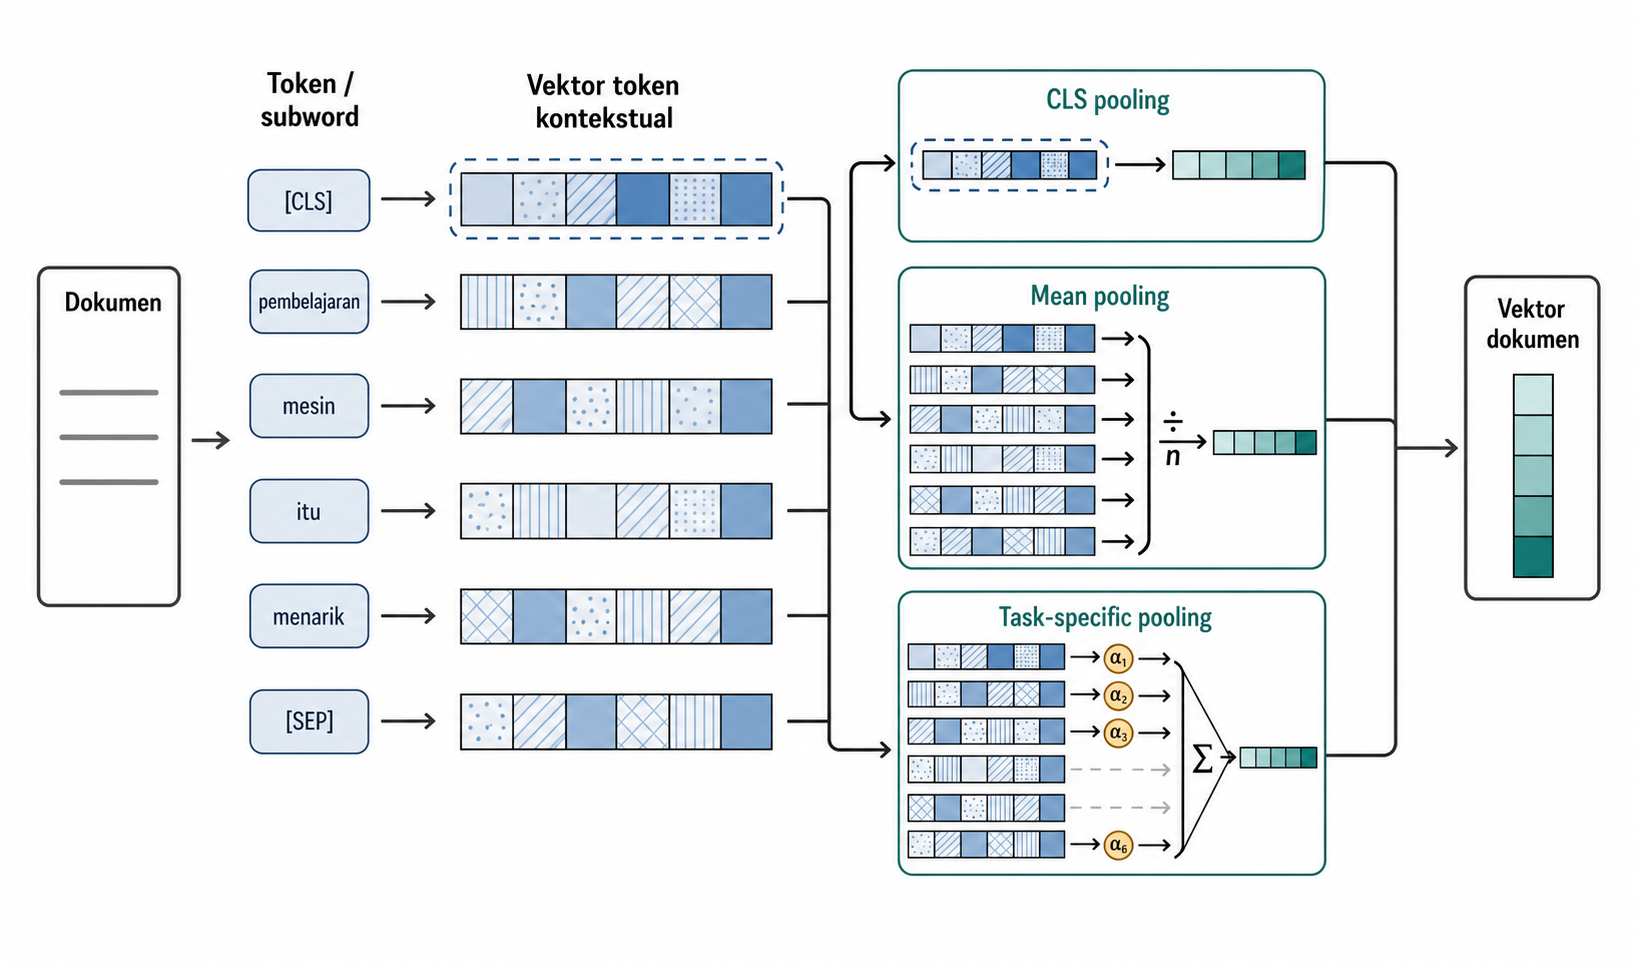
\includegraphics[width=111.6mm]{ch11-fig-3}
\caption{Dari dokumen ke vektor kalimat atau dokumen}
\label{fig:ch11-fig-3}
\end{figure}

Dokumen panjang membutuhkan strategi tambahan. Jika teks melebihi maximum length model, dokumen dapat dipotong, dibagi menjadi chunk, diringkas, atau diproses secara hierarkis. Untuk kumpulan abstrak skripsi, customer complaints, atau laporan medis, keputusan chunking dan pooling dapat sama pentingnya dengan model embedding yang dipilih.

Tabel 11.1 merangkum tangga representasi teks dari \emph{sparse} sampai \emph{contextual}. Makin ke bawah, representasi makin semantik dan kontekstual, tetapi biaya dan ketergantungan pada model juga meningkat. Dua bagian terakhir membandingkan representasi \emph{pretrained} yang dipakai secara beku dengan representasi yang diubah melalui \emph{fine-tuning}.

\tabeljudul{Tabel 11.1 — Tangga representasi teks}

{\def\LTcaptype{none} % do not increment counter
\par\vspace{3pt}\noindent
\begingroup\renewcommand{\arraystretch}{1.0}%
\scriptsize\linespread{1}\selectfont
\renewcommand{\_}{\textunderscore\hspace{0pt}}%
\begin{xltabular}{\linewidth}{@{}>{\raggedright\arraybackslash}p{(\linewidth-8\tabcolsep)*\real{0.160}} >{\raggedright\arraybackslash}p{(\linewidth-8\tabcolsep)*\real{0.222}} >{\raggedright\arraybackslash}p{(\linewidth-8\tabcolsep)*\real{0.160}} >{\raggedright\arraybackslash}p{(\linewidth-8\tabcolsep)*\real{0.227}} >{\raggedright\arraybackslash}p{(\linewidth-8\tabcolsep)*\real{0.231}}@{}}
\toprule

Representasi
 & 
Menangkap apa
 & 
Dimensi\slash{}bentuk
 & 
Kekuatan
 & 
Batas utama
 \\
\midrule
\endhead




BoW\slash{}n-gram & Kehadiran token dan urutan lokal pendek & Sparse, sebesar vocabulary & Kuat sebagai \emph{baseline}, mudah dijelaskan & Buta konteks dan sinonim \\
TF-IDF & Token yang khas bagi dokumen & Sparse berbobot & Kuat untuk klasifikasi\slash{}search kecil-menengah & Tidak memahami makna dan sinonim \\
Static word embedding & Kedekatan semantik token & Dense per token & Sinonim lebih dekat & Satu vektor untuk semua konteks \\
Contextual token embedding & Makna token dalam konteks & Dense per token\slash{}subword & Menangani polisemi & Perlu model besar dan pooling \\
Sentence\slash{}document embedding & Makna teks sebagai satu vektor & Dense per teks & Efisien untuk retrieval\slash{}klasifikasi & Pooling dan panjang dokumen menjadi isu \\
\bottomrule
\end{xltabular}\endgroup\par\vspace{5pt}

}

\section{\texorpdfstring{\emph{Pretrained Language Model} sebagai \emph{Feature Extractor}}{Pretrained Language Model sebagai Feature Extractor}}\label{pretrained-language-model-sebagai-feature-extractor}

Setelah representasi contextual dan document embedding masuk ke peta, pertanyaan praktisnya adalah bagaimana memakainya tanpa melatih model bahasa besar dari awal. \emph{Pretrained language model} dapat dipakai sebagai frozen feature extractor. Teks dimasukkan ke encoder, lalu hidden states atau pooled embedding diambil sebagai fitur. Setelah itu, model hilir yang lebih kecil, seperti logistic regression, SVM, atau gradient boosting, dilatih memakai label lokal. Encoder tidak diubah.

Pola ini adalah transfer. Representasi dipelajari dari korpus besar di luar proyek, lalu dipakai untuk tugas lokal. Keuntungannya ada pada efisiensi. Kita dapat memperoleh fitur semantik yang kuat tanpa melatih seluruh model bahasa. Jika data berlabel sedikit atau komputasi terbatas, frozen extraction sering lebih stabil daripada full fine-tuning.

Keuntungan lain adalah determinisme operasional. Encoder beku memetakan teks identik ke vektor identik selama versi model, tokenizer, pooling, maximum length, penskalaan vektor, dan batching dijaga sama. Ini memudahkan caching, debugging, dan audit. Fitur embedding dapat disimpan, dibandingkan, dan dipakai ulang selama definisinya jelas.

Namun, domain mismatch tetap penting. Model yang dilatih pada teks umum dapat kurang cocok untuk bahasa lokal, jargon kampus, dokumen hukum, catatan medis, OCR yang kotor, atau media sosial. Pada korpus dengan jargon berat, \emph{TF-IDF} sebagai \emph{baseline} yang disetel baik dapat mengalahkan embedding generik yang tidak pernah melihat istilah domain. Encoder yang diadaptasi domain dapat menutup jarak itu, tetapi harus dibuktikan melalui validasi lokal.

Feature extraction harus reproducible. Catat nama model, versi, tokenizer, layer atau pooling rule, maximum length, penskalaan vektor, dan cara batching. Jika salah satu berubah, fitur berubah. Dari sudut pandang Bab 9, embedding hasil ekstraksi adalah fitur yang perlu definisi, lineage, dan monitoring. Jika representasi beku belum cukup menyesuaikan makna domain, keputusan berikutnya adalah apakah bobot model perlu ikut dilatih.

\begin{pendalaman}{Memilih ekstraktor, MTEB dan ekosistem modern}
Massive Text Embedding Benchmark, atau MTEB, membandingkan embedding model pada banyak keluarga tugas sehingga pilihan extractor tidak hanya berbasis reputasi. Namun, skornya bersifat agregat. Validasi pada domain sendiri tetap wajib. Ekosistemnya bergerak cepat. Hidden states dari decoder-only LLM makin sering dipakai sebagai extractor, hybrid sparse-dense search menggabungkan lexical exactness dengan generalisasi semantik, dan model distilled menukar sedikit kualitas dengan penghematan inference. Semua ini adalah kandidat yang perlu diuji, bukan jaminan.
\end{pendalaman}

\section{\texorpdfstring{\emph{Fine-Tuning} vs \emph{Feature Extraction}}{Fine-Tuning vs Feature Extraction}}\label{fine-tuning-vs-feature-extraction}

Jika fitur beku belum cukup menyesuaikan makna domain, sebagian atau seluruh bobot model dapat dibuka. \emph{Feature extraction} membekukan encoder dan melatih model hilir atau \emph{head} dangkal. \emph{Fine-tuning} memperbarui sebagian atau seluruh bobot model \emph{pretrained} memakai data tugas. Perbedaannya juga menyangkut keputusan representasi, yaitu apakah pengetahuan bahasa yang ada sudah cukup atau model perlu diubah agar sesuai dengan domain dan label lokal.

Full fine-tuning dapat menyesuaikan model lebih kuat. Contohnya, kata ``positif'' dalam sentimen umum sering bernilai baik, tetapi ``tumor positif'' dalam teks medis berarti kabar buruk. Frozen general embedding mungkin tidak cukup menyesuaikan makna seperti ini. Fine-tuning dapat menggeser representasi agar sesuai dengan label domain, asalkan data dan validasinya memadai.

Namun, \emph{fine-tuning} membutuhkan lebih banyak data, komputasi, dan pengendalian \emph{overfitting}. Jumlah label saja bukan ambang keputusan. Bandingkan ekstraksi beku, PEFT, dan \emph{full fine-tuning} melalui validasi lokal dengan mempertimbangkan ukuran model, pergeseran domain, kualitas dan keseimbangan label, regularisasi, serta anggaran komputasi. \emph{Parameter-efficient adaptation} seperti LoRA dan kerabatnya menjadi pilihan antara karena hanya melatih sebagian kecil parameter tambahan. Metode \emph{few-shot} seperti SetFit juga dapat diuji ketika label terbatas. Detailnya dibahas pada Bab 15.

Gambar 11.4 membandingkan alur gradient. Pada frozen extraction, gradient berhenti di batas encoder. Hanya model hilir yang dilatih. Pada fine-tuning, gradient mengalir sampai bobot encoder. Jalur PEFT berada di tengah karena sebagian adapter kecil dilatih, sedangkan sebagian besar bobot tetap.

\begin{figure}[tbp]\centering
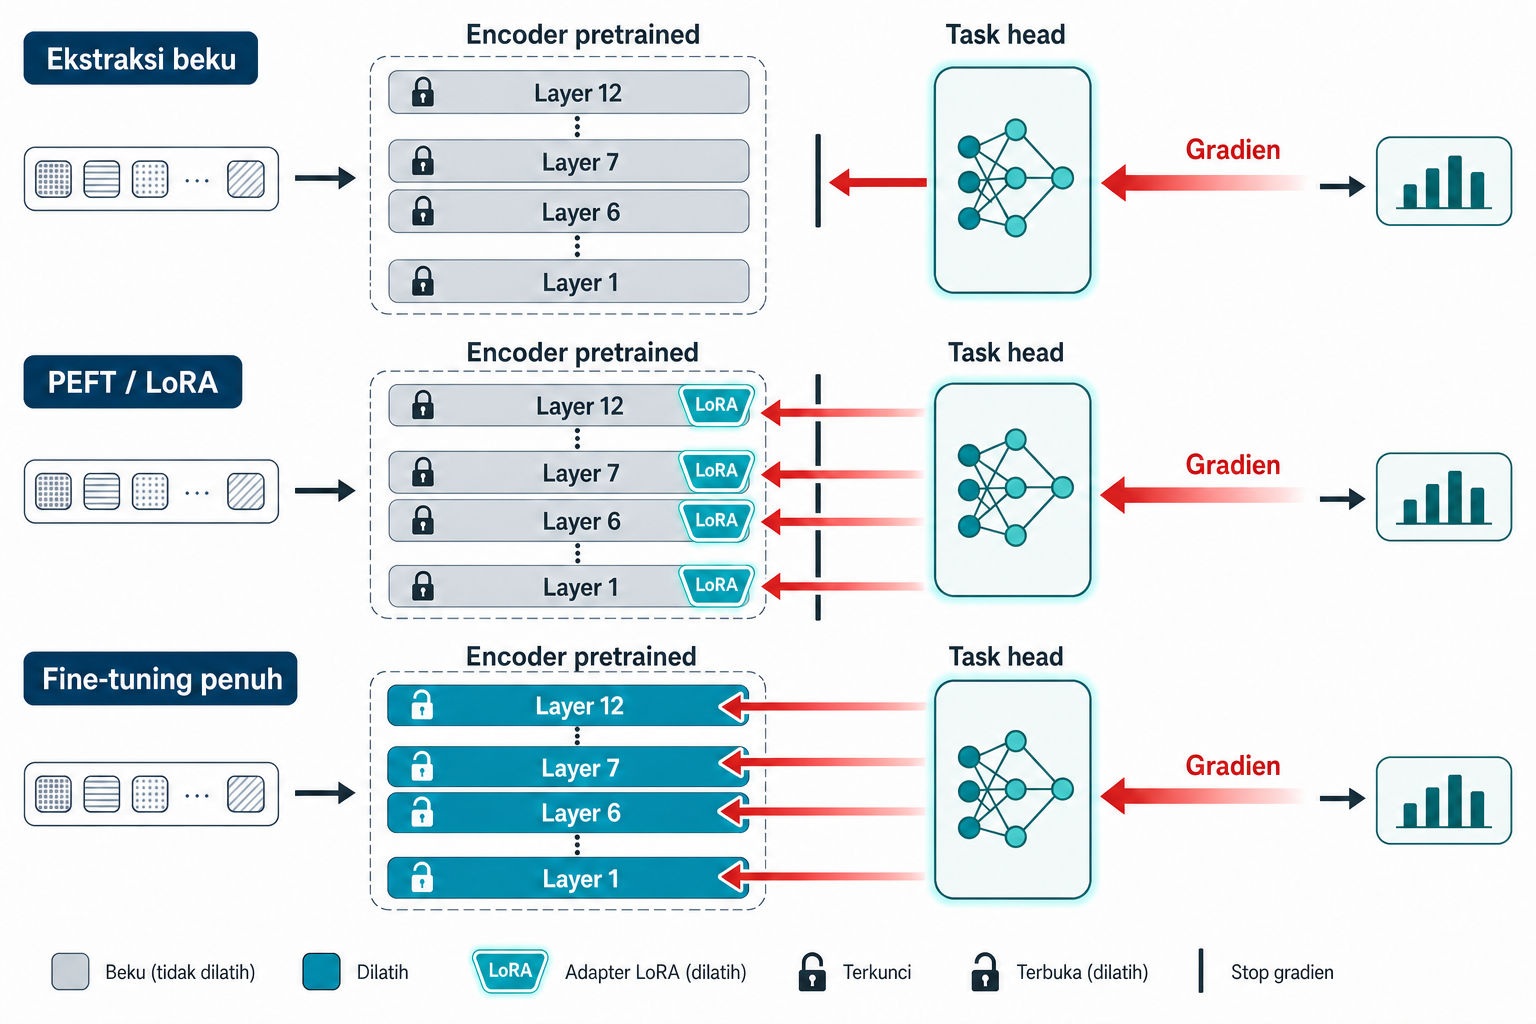
\includegraphics[width=111.6mm]{ch11-fig-4}
\caption{Ekstraksi beku dan fine-tuning}
\label{fig:ch11-fig-4}
\end{figure}

Keputusan antara ekstraksi dan fine-tuning bergantung pada ukuran data, domain mismatch, kualitas label, latency, interpretabilitas, komputasi, dan kebutuhan pemeliharaan. Tabel 11.2 merangkum beberapa situasi umum.

\tabeljudul{Tabel 11.2 — Feature extraction vs fine-tuning}

{\def\LTcaptype{none} % do not increment counter
\par\vspace{3pt}\noindent
\begingroup\renewcommand{\arraystretch}{1.0}%
\scriptsize\linespread{1}\selectfont
\renewcommand{\_}{\textunderscore\hspace{0pt}}%
\begin{xltabular}{\linewidth}{@{}>{\raggedright\arraybackslash}p{(\linewidth-6\tabcolsep)*\real{0.236}} >{\raggedright\arraybackslash}p{(\linewidth-6\tabcolsep)*\real{0.266}} >{\raggedright\arraybackslash}p{(\linewidth-6\tabcolsep)*\real{0.203}} >{\raggedright\arraybackslash}p{(\linewidth-6\tabcolsep)*\real{0.295}}@{}}
\toprule

Situasi
 & 
Cenderung ke ekstraksi beku
 & 
Cenderung ke fine-tuning
 & 
Perhatian
 \\
\midrule
\endhead




Dataset berlabel kecil & Ya & Tidak, kecuali adaptasi ringan & Risiko overfitting tinggi \\
Dataset in-domain besar & Bisa sebagai \emph{baseline} & Ya & Butuh validasi dan compute \\
Latensi ketat & Ya, embedding dapat di-cache & Mungkin mahal & Ukur inference end-to-end \\
Kesenjangan domain kuat & \emph{Baseline} perlu diuji & Ya, jika label cukup & Jargon dapat mengubah makna \\
Butuh \emph{baseline} interpretable & TF-IDF \slash{} fitur sparse lebih mudah & Tidak utama & Bandingkan dengan \emph{baseline} klasik \\
\bottomrule
\end{xltabular}\endgroup\par\vspace{5pt}

}

Validasi teks punya kegagalan khas. Vocabulary leakage terjadi ketika vectorizer lokal di-\emph{fit} pada seluruh korpus sebelum split, sehingga token validasi sudah masuk vocabulary dan bobot. Cross-split duplication terjadi ketika artikel sindikasi, review bot, atau dokumen hampir sama tersebar di train dan validasi. Model tampak memahami bahasa, padahal hanya menghafal. Audit duplikat lebih dulu, lalu pilih deduplikasi atau pemisahan grup sesuai protokol penerapan. Pada contoh SMS Spam, teks ternormalisasi dapat dijadikan grup agar pesan duplikat tidak melintasi \emph{split}; korpus lain dapat memerlukan pengelompokan berdasarkan sumber atau penulis, atau pemisahan waktu jika kronologinya memang tersedia.

Jadi, perdebatan utamanya bukan representasi klasik versus modern. Untuk dataset kecil, domain jargon, kebutuhan interpretasi, atau \emph{baseline} cepat, \emph{TF-IDF} dan model linear masih sangat layak. Representasi modern harus mengalahkan \emph{baseline} yang dibangun baik, bukan hanya terlihat lebih canggih.

\begin{sintesis}

Benang merah Bab 11 adalah bahwa teks tidak pernah masuk ke model sebagai string mentah yang netral. Teks selalu diterjemahkan menjadi representasi, dan terjemahan itu menentukan apakah model menerima hitungan token, bobot dokumen, kedekatan semantik, konteks, atau makna dokumen secara utuh.

Representasi klasik seperti \emph{bag-of-words}, \emph{n-gram}, dan \emph{TF-IDF} tetap kuat sebagai \emph{baseline} karena sederhana, sparse, dan relatif mudah dijelaskan. Word embedding dan contextual embedding menambahkan geometri semantik dan konteks, tetapi bergantung pada korpus, tokenizer, pooling, dan model yang dipilih. Tabel 11.1 merangkum tangga ini sebagai peta representasi.

Pada ujung modern, \emph{pretrained language model} memperluas pilihan tetapi tidak menghapus keputusan rekayasa fitur. Tabel 11.2 membantu menimbang ukuran data, kesenjangan domain, \emph{latency}, dan kebutuhan interpretasi. Tabel tersebut menunjukkan kapan embedding beku cukup sebagai fitur dan kapan adaptasi bobot layak dibayar. Representasi teks harus dipasang dalam validasi yang benar, dibandingkan dengan \emph{baseline} yang kuat, dan didokumentasikan agar dapat direproduksi.

\end{sintesis}

\begin{bacaan}

\begin{itemize}
\tightlist
\item
  scikit-learn --- Text feature extraction --- \url{https://scikit-learn.org/stable/modules/feature_extraction.html\#text-feature-extraction}. Bag-of-words dan TF-IDF.
\item
  Mikolov dkk. (2013), Word2Vec --- \url{https://arxiv.org/abs/1301.3781}. Embedding kata dari konteks.
\item
  Bojanowski dkk. (2017), fastText --- \url{https://arxiv.org/abs/1607.04606}. Embedding subword untuk kata langka.
\item
  Devlin dkk. (2019), BERT --- \url{https://arxiv.org/abs/1810.04805}. Embedding kontekstual dari transformer.
\item
  Reimers \& Gurevych (2019), Sentence-BERT --- \url{https://arxiv.org/abs/1908.10084}. Embedding kalimat untuk kemiripan.
\item
  Robertson \& Zaragoza (2009), BM25 --- \url{https://doi.org/10.1561/1500000019}. Fungsi pemeringkatan pencarian klasik.
\item
  Muennighoff dkk. (2022), MTEB --- \url{https://arxiv.org/abs/2210.07316}. Tolok ukur embedding teks.
\item
  Tunstall dkk. (2022), SetFit --- \url{https://arxiv.org/abs/2209.11055}. Fine-tuning few-shot untuk klasifikasi teks.
\end{itemize}

\end{bacaan}

\rujukanheading

\protect\phantomsection\label{refs}
\begin{CSLReferences}{1}{1}
\bibitem[\citeproctext]{ref-devlin2019bert}
Devlin, Jacob, Ming-Wei Chang, Kenton Lee, and Kristina Toutanova. 2019. {``{BERT}: Pre-Training of Deep Bidirectional Transformers for Language Understanding.''} \emph{Proceedings of the 2019 Conference of the North American Chapter of the Association for Computational Linguistics (NAACL-HLT)}.

\bibitem[\citeproctext]{ref-mikolov2013word2vec}
Mikolov, Tomas, Kai Chen, Greg Corrado, and Jeffrey Dean. 2013. \emph{Efficient Estimation of Word Representations in Vector Space}. \url{https://arxiv.org/abs/1301.3781}.

\bibitem[\citeproctext]{ref-reimers2019sbert}
Reimers, Nils, and Iryna Gurevych. 2019. {``Sentence-{BERT}: Sentence Embeddings Using Siamese {BERT}-Networks.''} \emph{Proceedings of the 2019 Conference on Empirical Methods in Natural Language Processing (EMNLP)}.

\bibitem[\citeproctext]{ref-saltonbuckley1988tfidf}
Salton, Gerard, and Christopher Buckley. 1988. {``Term-Weighting Approaches in Automatic Text Retrieval.''} \emph{Information Processing \& Management} 24 (5): 513--23.

\end{CSLReferences}

% ==========================================================================
% ch12.tex — dihasilkan otomatis dari website/chapters/ch12.qmd
% Boleh disunting manual. 'sync' hanya menimpa bila .qmd berubah DAN .tex
% belum disunting; kalau keduanya berubah, dilewati (pakai --force).
% qmd-sha1: f01f4d5e99a6
% tex-sha1: 3a4b9fd4437f
% ==========================================================================
% >>>>> ISI OTOMATIS (jangan hapus baris ini) >>>>>
\chapter{Citra \& Audio}\label{citra-audio}

\section{Citra: Normalisasi dan Augmentasi}\label{citra-normalisasi-dan-augmentasi}

Data citra digital pada dasarnya merupakan matriks numerik spasial berdimensi tinggi. Sebuah gambar berwarna tersusun atas kisi dua dimensi yang merekam tiga kanal warna (RGB), dengan setiap titik piksel menyimpan nilai intensitas dari 0 hingga 255. Sebelum arsitektur \emph{computer vision} dapat mengekstraksi representasi polanya, data mentah ini harus distandarkan melalui dua mekanisme utama: normalisasi dan augmentasi.

\textbf{Normalisasi Citra}
Normalisasi menstandarkan rentang nilai piksel untuk memastikan gradien algoritma \emph{machine learning} tetap stabil saat konvergensi. Praktik industri modern umumnya menerapkan standardisasi \emph{Z-score} per kanal warna melalui persamaan \( x_{c}^{\text{norm}} = \frac{x_c - \mu_c}{\sigma_c} \). Dalam rumusan tersebut, \(x_c\) mewakili intensitas piksel asli pada kanal warna spasial \(c\) (misalnya merah, hijau, atau biru), \(\mu_c\) menyatakan rata-rata intensitas piksel, dan \(\sigma_c\) merepresentasikan simpangan bakunya pada kanal tersebut. Untuk menjaga integritas \emph{pipeline}, parameter rata-rata dan simpangan baku wajib dihitung secara eksklusif dari himpunan data latih. Konstanta ini kemudian dikunci dan diaplikasikan pada data pengujian. Apabila menggunakan \emph{pretrained model}, praktisi harus menormalisasi citra mengikuti distribusi statistik asal model tersebut, seperti konstanta rata-rata standar ImageNet \passthrough{\lstinline![0.485, 0.456, 0.406]!}.

\textbf{Augmentasi Data}
Augmentasi menyisipkan transformasi sintetis di dalam \emph{pipeline} untuk mencegah model menghafal tata letak piksel (\emph{overfitting}). Transformasi ini secara khusus hanya dijalankan pada fase pelatihan. Teknik augmentasi mencakup manipulasi geometris dan visual dasar, seperti pemotongan acak, pembalikan horizontal, distorsi prespektif, dan injeksi \emph{noise} warna. Selain itu, kerangka kerja modern menggunakan kebijakan otomatis (\emph{AutoAugment} atau \emph{RandAugment}) yang secara acak mengundi kombinasi transformasi dari kumpulan prosedur operasi standar. Terdapat juga pendekatan tingkat lanjut seperti augmentasi lintas sampel (\emph{Mixup} atau \emph{CutMix}) yang menggabungkan potongan citra dari kelas berbeda untuk melatih model memprediksi rasio probabilitas gabungan, sehingga model difokuskan pada morfologi lokal dibandingkan latar belakang global.

Kedua tahapan prapemrosesan ini menentukan apakah representasi fitur dapat mengekstraksi objek dengan konsisten atau terdistorsi oleh variasi pencahayaan.

\section{Fitur Rancangan Tangan (HOG) dan Keterbatasannya}\label{fitur-rancangan-tangan-hog-dan-keterbatasannya}

Sebelum representasi mendalam digunakan secara luas, pemahaman citra bertumpu pada representasi rancangan manusia. Pendekatan ini menghindari penggunaan piksel mentah yang sensitif terhadap perubahan cahaya atau pergeseran posisi. Pergeseran pencahayaan dapat mengubah susunan angka piksel secara drastis, meskipun objek yang ditangkap tetap sama. Ekstraksi fitur difokuskan pada perhitungan lokal yang memanfaatkan operasi matematika untuk mendeteksi tepian atau sudut pada area kecil gambar. Hasil perhitungan tersebut mengubah matriks piksel menjadi vektor fitur yang konsisten terhadap gangguan visual lingkungan.

Contoh paling menonjol dari pendekatan ini adalah algoritma \emph{Histogram of Oriented Gradients} (HOG). Algoritma ini membagi citra ke dalam kisi-kisi blok berukuran kecil dan menghitung arah perubahan intensitas warna (\emph{gradient}). Dalam kalkulasi ini, gradien citra dihitung berdasarkan perbedaan intensitas antara piksel yang bersebelahan. Jika \(I(x,y)\) mewakili intensitas piksel pada koordinat \((x,y)\), komponen gradien horizontal (\(G_x\)) dan vertikal (\(G_y\)) dirumuskan sebagai \(G_x = I(x+1, y) - I(x-1, y)\) dan \(G_y = I(x, y+1) - I(x, y-1)\). Variabel \(G_x\) mengukur perubahan intensitas secara horizontal untuk memetakan tepian vertikal, sedangkan \(G_y\) mengukur perubahan vertikal untuk memetakan tepian horizontal. Dari kedua nilai tersebut, algoritma HOG menghitung magnitudo dan orientasi arah gradien untuk menyusun siluet kontur fisik objek.

\begin{figure}[htbp]\centering
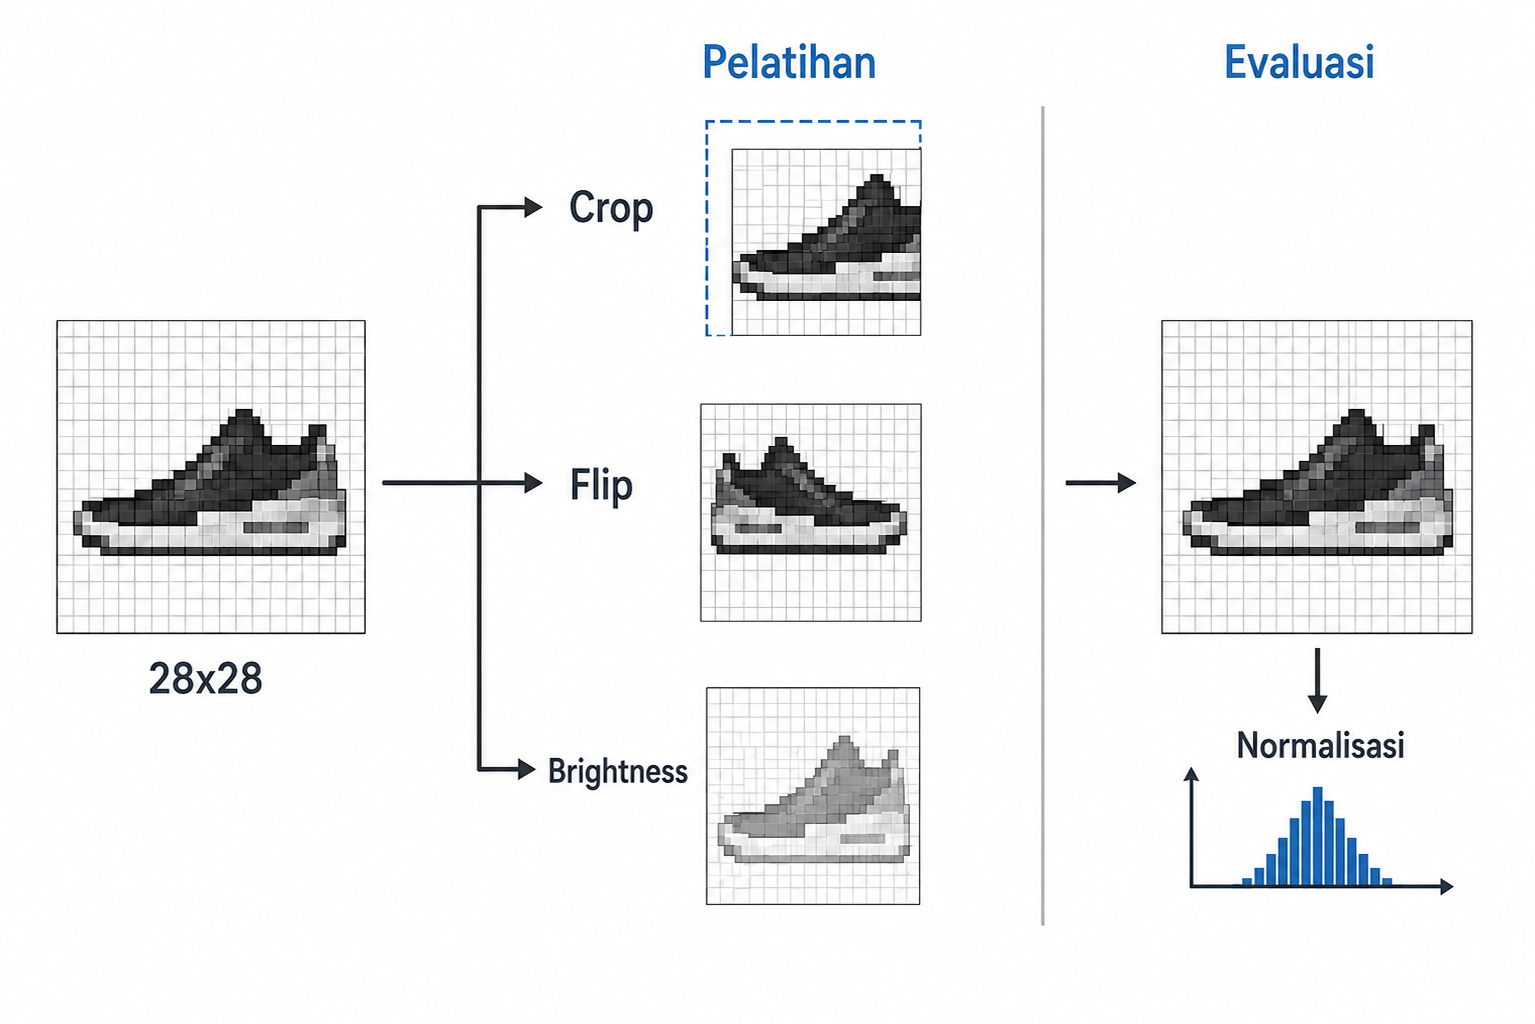
\includegraphics[width=\linewidth,height=0.72\textheight,keepaspectratio]{ch12-fig-1}
\caption{Ekstraksi Fitur Histogram of Oriented Gradients (HOG) pada Citra}
\label{fig:ch12-fig-1}
\end{figure}

Pada kasus deteksi pejalan kaki, model tidak mengevaluasi warna pakaian target. Ekstraktor HOG memetakan siluet target dengan mengidentifikasi garis vertikal tubuh serta lengkungan kepala melalui nilai gradien. Perhitungan tersebut kemudian dikelompokkan ke dalam blok-blok spasial berukuran tetap. Algoritma merangkum dominasi arah gradien tersebut ke dalam sebuah histogram distribusi orientasi lokal. Representasi spasial ini bertindak sebagai fitur akhir, sehingga target terdeteksi secara konsisten di dalam ruang gradien HOG tanpa terpengaruh variasi visual pakaian.

Pendekatan ekstraksi manual ini memiliki keterbatasan struktural. Pembuatan algoritma menuntut pemahaman domain spesifik mengenai manipulasi citra dan proses rekayasa parametrik. Parameter sistem seperti dimensi sel, ukuran blok, dan ambang batas intensitas harus dikonfigurasi secara manual untuk target deteksi yang berbeda. Selain itu, fitur rancangan tangan tidak memetakan konteks tingkat tinggi. HOG memetakan batas siluet objek dengan baik, tetapi tidak mampu menyerap konteks semantik, seperti membedakan objek fisik dari gambar dua dimensi. Keterbatasan ini memfasilitasi transisi penggunaan representasi yang dipelajari secara langsung dari data pelatihan.

\section{\texorpdfstring{CNN \emph{Feature Extractor} dan \emph{Pretrained Model}}{CNN Feature Extractor dan Pretrained Model}}\label{cnn-feature-extractor-dan-pretrained-model}

Pemrosesan citra berkembang secara signifikan melalui arsitektur \emph{Convolutional Neural Network} (CNN) yang memfasilitasi ekstraksi representasi melalui pembelajaran mesin. Algoritma ini memetakan pola visual dari data pelatihan tanpa menggunakan aturan matematis yang statis. CNN bekerja dengan menggeser sekumpulan filter melintasi area citra untuk mengekstraksi berbagai fitur. Operasi konvolusi dasar dirumuskan sebagai \( \mathbf{Y}_{i,j} = \sum_{m} \sum_{n} \mathbf{W}_{m,n} \cdot \mathbf{X}_{i+m, j+n} \). Dalam perumusan tersebut, \(\mathbf{Y}\) melambangkan \emph{feature map} keluaran, \(\mathbf{W}\) merupakan matriks filter pembawa bobot yang dioptimalkan selama pelatihan, dan \(\mathbf{X}\) merepresentasikan area piksel citra masukan.

Melalui operasi konvolusi berulang, CNN membangun pemahaman visual secara hierarkis. Pada lapisan awal, filter merespons komponen spasial sederhana seperti garis vertikal, sudut, lengkungan, dan gradasi warna. Pada lapisan menengah, jaringan menyatukan komponen tersebut menjadi struktur tekstur atau fitur spesifik objek. Pada lapisan dalam, fitur parsial dikonsolidasi menjadi representasi semantik tingkat tinggi yang membedakan objek secara utuh. Kemampuan pembelajaran berjenjang ini mendukung implementasi \emph{transfer learning}. CNN yang telah dilatih dengan jutaan citra memiliki representasi spasial yang universal. Model dasar ini bertindak sebagai \emph{pretrained model}, di mana kemampuan ekstraksinya digunakan kembali untuk mengevaluasi domain data baru.

\begin{figure}[htbp]\centering
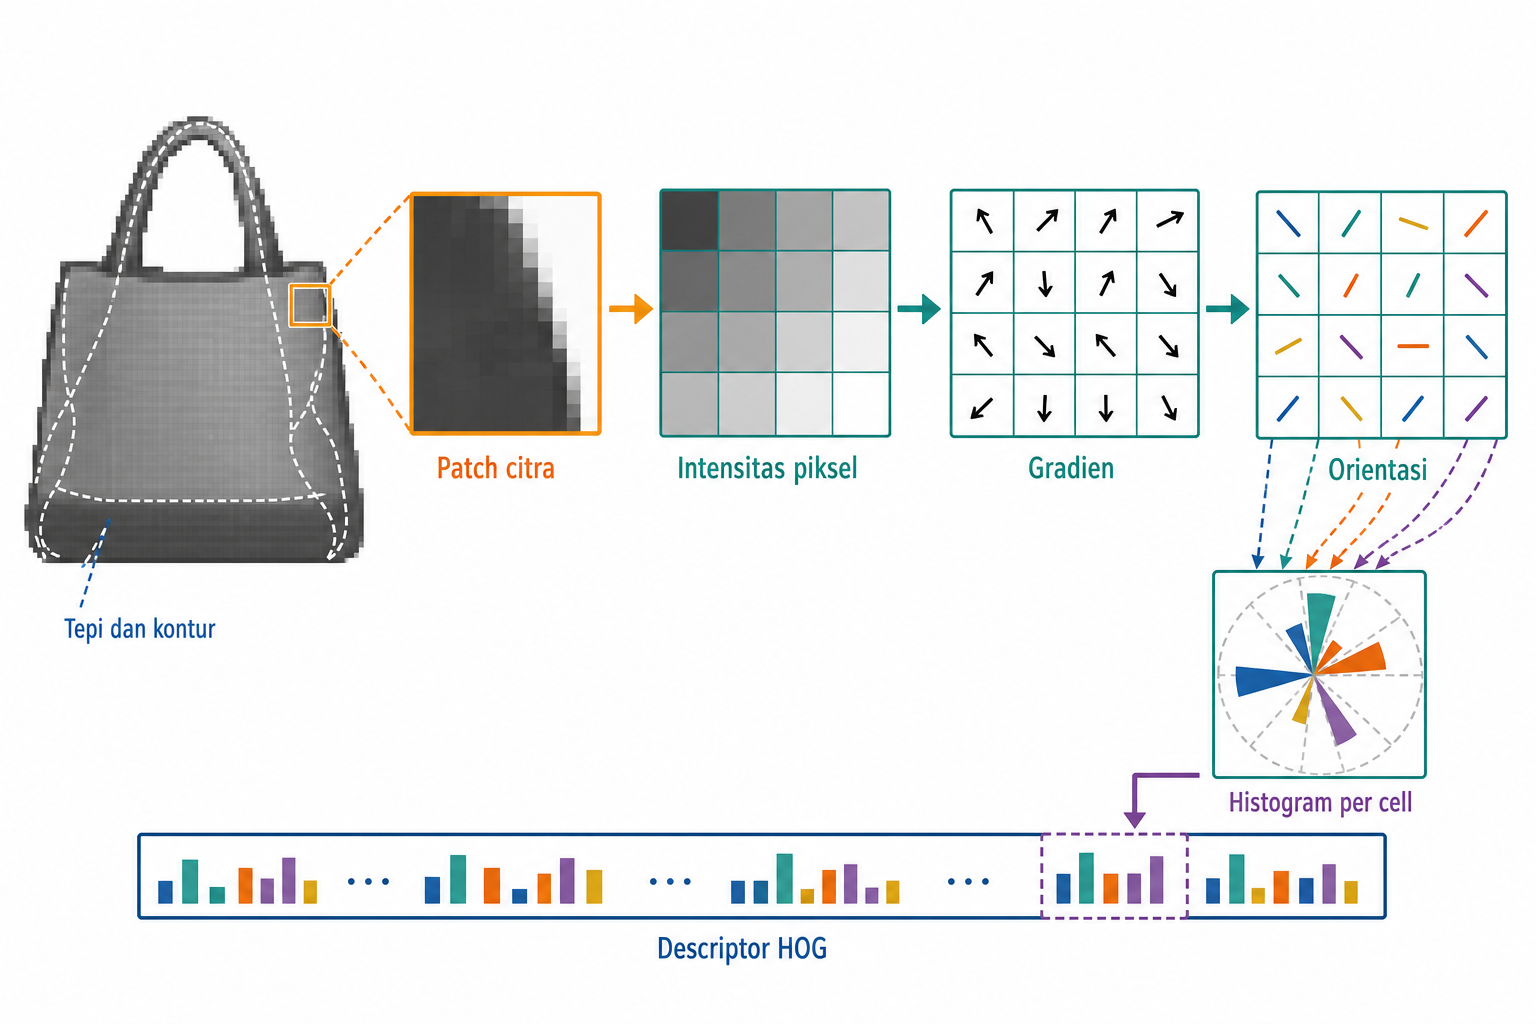
\includegraphics[width=\linewidth,height=0.72\textheight,keepaspectratio]{ch12-fig-2}
\caption{Arsitektur CNN Menghilangkan Lapisan Klasifikasi Akhir Menjadi Feature Extractor}
\label{fig:ch12-fig-2}
\end{figure}

Dalam implementasinya, varian arsitektur seperti ResNet dapat dimodifikasi dengan menghilangkan lapisan klasifikasi akhir. Sisa jaringan dialihfungsikan sebagai \emph{feature extractor} murni. Ketika citra medis atau foto industri dimasukkan ke dalam jaringan ini, model tidak memprediksi probabilitas kelas, melainkan memproduksi vektor fitur yang memuat representasi visual citra. Vektor inilah yang kemudian dialirkan ke model prediktif sederhana untuk mendeteksi anomali. Pendekatan ini menghasilkan representasi dengan akurasi tinggi tanpa mengharuskan sistem melatih parameter dari awal.

Meskipun model berbasis \emph{Vision Transformer} (ViT) menjadi standar alternatif yang populer, CNN tetap dipertahankan pada lini komputasi industri. Evaluasi empiris menunjukkan bahwa arsitektur CNN seperti ConvNeXt v2 memiliki kinerja yang sebanding atau mengungguli ViT pada himpunan data berukuran menengah. Struktur operasi konvolusi memungkinkan model mengekstraksi informasi visual dengan efisien saat ketersediaan data pelatihan sangat terbatas.

\section{Image Embedding dan Patch}\label{image-embedding-dan-patch}

Arsitektur \emph{Vision Transformer} (ViT) menyediakan pendekatan alternatif yang memproses seluruh area citra sebagai urutan sekuensial. Langkah awal metode ini membagi citra menjadi kumpulan \emph{patch} persegi yang diletakkan berdampingan tanpa tumpang tindih. Setiap \emph{patch} kemudian diratakan dan diproses sebagai sebuah \emph{token} independen, yang memiliki peran identik dengan representasi kata dalam model bahasa. Pemotongan area spasial ini dirumuskan melalui persamaan \( N = \frac{H \times W}{P^2} \). Dalam persamaan tersebut, \(N\) menyatakan total \emph{patch} keluaran, \(H\) dan \(W\) mewakili dimensi tinggi dan lebar citra asli, serta \(P\) merepresentasikan ukuran sisi setiap \emph{patch}. Sebagai contoh, citra beresolusi 224×224 piksel dengan ukuran \emph{patch} 16×16 piksel akan direpresentasikan menjadi 256 \emph{patch} terpisah.

Komponen komputasi \emph{attention} mengevaluasi keterkaitan seluruh \emph{token} tersebut secara bersamaan. Mekanisme ini memfasilitasi identifikasi korelasi antara objek yang terpisah secara spasial dalam satu gambar.

\begin{figure}[htbp]\centering
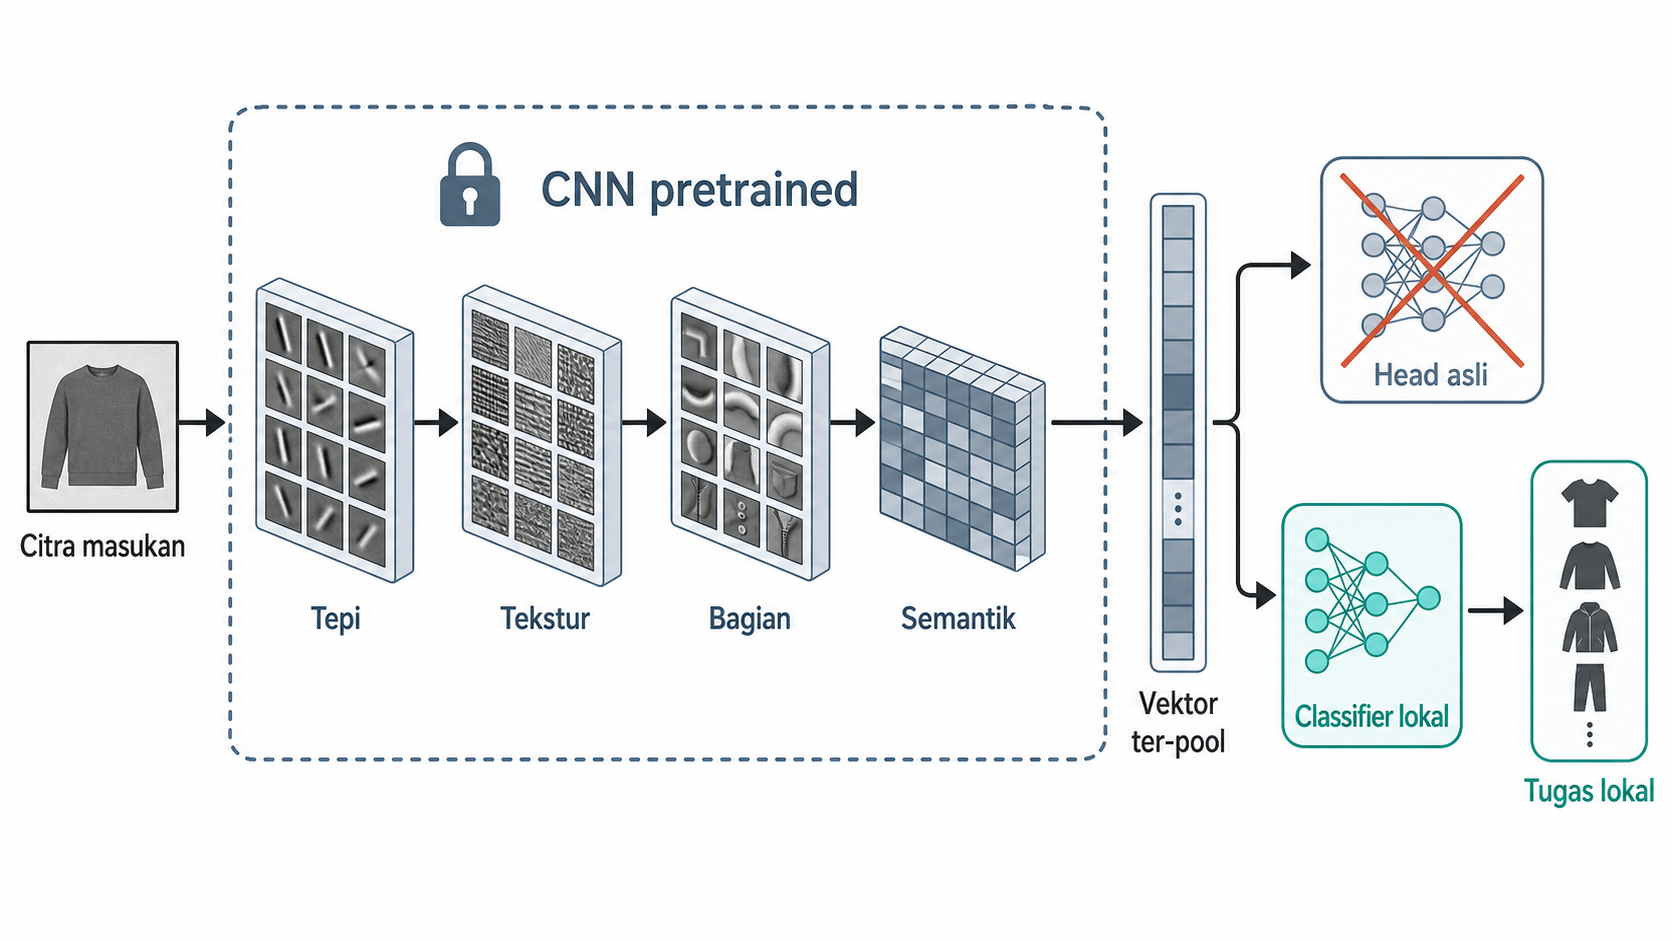
\includegraphics[width=\linewidth,height=0.72\textheight,keepaspectratio]{ch12-fig-3}
\caption{Pemotongan Citra Menjadi Kisi Patch dan Mekanisme Attention pada Vision Transformer}
\label{fig:ch12-fig-3}
\end{figure}

Pemrosesan relasi antarkepingan ini mengonsolidasi makna semantik visual ke dalam ruang kontinu tunggal yang disebut \emph{image embedding}. Representasi ini memetakan konsep objek secara utuh. Jika dua citra menampilkan kelas objek yang sama, vektor \emph{embedding} dari keduanya akan dipetakan berdekatan secara matematis tanpa dipengaruhi oleh variasi latar belakang visual.

Dalam praktik rekayasa fitur modern, terdapat beberapa keluarga \emph{pretrained model} yang menjadi standar ekstraksi citra. Model keluarga CLIP dan SigLIP dilatih menggunakan jutaan pasangan citra dan teks, dengan bagian \emph{encoder} visual dari SigLIP sering digunakan sebagai pengekstraksi fitur serbaguna karena memiliki rentang representasi yang lebih umum dibanding arsitektur konvensional. Alternatif lainnya adalah DINOv2, arsitektur \emph{self-supervised learning} yang dioptimalkan untuk mengekstraksi struktur spasial. DINOv2 memproduksi \emph{token} CLS yang merangkum \emph{image embedding} global, bersama fitur tingkat \emph{patch} yang mendukung resolusi tinggi untuk memfasilitasi tugas prediksi padat seperti segmentasi spasial. Untuk aplikasi tingkat lanjut, fitur direpresentasikan menggunakan pendekatan multi-skala dan hibrida. Arsitektur modern seperti ConvNeXt v2 menggabungkan hierarki CNN dengan protokol pelatihan transformer untuk mengompilasi fitur yang merekam detail lokal dan konteks global sekaligus.

Pendekatan sekuensial ini menyelaraskan pemrosesan data lintas modalitas, di mana representasi visual dan tekstual disatukan menggunakan struktur komputasi yang seragam pada arsitektur pembelajaran multimodal.

\section{Audio: Waveform, Spektrogram, MFCC, dan Chroma}\label{audio-waveform-spektrogram-mfcc-dan-chroma}

Data audio pada dasarnya merupakan sinyal \emph{waveform} mentah berdimensi tunggal yang mencatat perubahan amplitudo tekanan udara seiring waktu. Pada setiap titik temporal, berbagai sumber suara berakumulasi menjadi satu nilai amplitudo. Mengingat sinyal ini menuntut pemisahan komponen akustik, pendekatan klasik merancang transformasi untuk mengonversi sinyal dari domain waktu ke domain frekuensi melalui spektrogram. Transformasi ini memetakan fluktuasi satu dimensi menjadi representasi visual dua dimensi. Rentang waktu diposisikan pada sumbu horizontal, frekuensi pada sumbu vertikal, dan amplitudo direpresentasikan melalui intensitas piksel. Perubahan format menjadi citra spektrum memfasilitasi penerapan algoritma \emph{computer vision} pada data audio.

Untuk memodelkan persepsi pendengaran biologis, dirancang representasi frekuensi yang mengikuti skala Mel. Pendengaran manusia beroperasi secara non-linear, menunjukkan sensitivitas tinggi terhadap pergeseran nada pada frekuensi rendah dan penurunan sensitivitas pada frekuensi tinggi. Korelasi antara frekuensi asli dengan skala Mel dinyatakan melalui persamaan \( m = 2595 \log_{10} \left( 1 + \frac{f}{700} \right) \). Dalam perumusan tersebut, \(m\) menyatakan frekuensi pada skala Mel dan \(f\) menyatakan frekuensi aktual dalam satuan Hertz.

Berdasarkan konversi persepsi tersebut, terdapat beberapa teknik ekstraksi fitur spesifik untuk pemrosesan audio. Mel-spektrogram memetakan sumbu frekuensi ke skala Mel sambil mempertahankan dimensi spasial komponen suara, menjadikannya format standar bagi pengklasifikasi audio berbasis CNN. Teknik \emph{Mel-Frequency Cepstral Coefficients} (MFCC) menghasilkan representasi yang mengekstraksi selubung spektrum suara dari Mel-spektrogram. MFCC umumnya diimplementasikan ketika data latih berjumlah kecil untuk pemodelan klasik, atau pada arsitektur \emph{edge deployment} dengan kendala memori. Untuk analisis musik, \emph{chroma feature} meringkas energi frekuensi ke dalam dua belas kelas nada dasar. Teknik ini mengeliminasi informasi oktaf untuk menonjolkan identitas harmoni, sehingga mendukung inferensi progresi kord dan klasifikasi genre lagu. 

Teknik-teknik ekstraksi ini merepresentasikan fitur berbasis rancangan manusia yang digunakan untuk mereduksi dimensi sekaligus mengisolasi pola sinyal akustik sebelum dievaluasi oleh sistem prediktif.

\section{Pretrained Audio Encoder: Model Raw-Waveform}\label{pretrained-audio-encoder-model-raw-waveform}

Pemrosesan audio mutakhir menggunakan representasi yang dipelajari mesin untuk mengolah \emph{raw waveform} secara langsung. Arsitektur \emph{state-of-the-art} mengekstrak pola akustik dari fluktuasi amplitudo tanpa menggunakan transformasi domain frekuensi statis. Model \emph{raw-waveform} seperti wav2vec 2.0 dan HuBERT memproses deret amplitudo 1D menggunakan tumpukan konvolusi 1D. Alih-alih mengekstraksi fitur diskrit melalui konversi tetap, model ini menggunakan matriks bobot yang dioptimalkan dari data pelatihan untuk memetakan gelombang suara menjadi matriks fitur kontinu.

Peningkatan metrik arsitektur ini didukung oleh metode \emph{self-supervised learning} (SSL). Selama pelatihan, model mengevaluasi puluhan ribu jam rekaman wicara tanpa label. Sistem menerapkan penyembunyian (\emph{masking}) pada sebagian segmen deret representasi, dan model dioptimalkan untuk memprediksi fitur dari porsi yang disembunyikan. Tugas rekonstruksi ini memungkinkan model mengenali hierarki fonetik secara otonom.

Implementasi rekayasa fitur saat ini bergeser pada penggunaan \emph{pretrained model} untuk menghasilkan vektor representatif. Keluarga model wav2vec 2.0 dan HuBERT bertindak sebagai standar untuk tugas pengenalan ucapan (\emph{speech recognition}), dengan iterasi besar seperti Wav2Vec2-BERT 2.0 yang dilatih menggunakan jutaan jam audio. Model WavLM mengembangkan arsitektur HuBERT menggunakan mekanisme pencampuran ucapan (\emph{utterance mixing}) untuk menahan retensi identitas pembicara, yang diutamakan pada tugas \emph{speaker verification}. Pada klasifikasi alternatif, status tersembunyi (\emph{hidden state}) dari blok akhir \emph{encoder} model Whisper digunakan sebagai pengekstraksi fitur semantik. Selain arsitektur wicara, terdapat model spesifik-domain seperti AudioMAE dan BEATs yang dikalibrasi untuk pengenalan kejadian suara lingkungan (\emph{sound event detection}), serta model MERT untuk mengekstraksi fitur kemusikan.

Pada tahapan pra-pemrosesan, rentang sampel \emph{waveform} distandarkan durasinya melalui pemotongan atau penambahan bantalan (\emph{padding}), dan laju sampelnya (\emph{sampling rate}) diseragamkan ke batas spesifikasi arsitektur sebelum dievaluasi oleh \emph{encoder}. Keluaran dari tahap ini kemudian difungsikan sebagai masukan bagi klasifikasi hilir.

\section{\texorpdfstring{\emph{Audio Embedding} dan Agregasi Sepanjang Waktu}{Audio Embedding dan Agregasi Sepanjang Waktu}}\label{audio-embedding-dan-agregasi-sepanjang-waktu}

Rekaman audio memuat dimensi temporal melintasi deret waktu. Pemrosesan rekaman melalui ekstraktor fitur menghasilkan rentetan matriks observasi dalam orde milidetik. Karakteristik sekuensial ini menuntut mekanisme agregasi, mengingat pengklasifikasi hilir (\emph{downstream classifier})—seperti model deteksi kelas suara—membutuhkan masukan dengan dimensi statis yang tidak bergantung pada panjang durasi asli. Deretan fitur tingkat \emph{frame} dikompresi menjadi vektor representatif tunggal yang disebut \emph{audio embedding}.

Pemadatan (\emph{pooling}) representasi temporal ini dieksekusi melalui beberapa mekanisme agregasi. Metode \emph{average pooling} menghitung nilai rata-rata dari seluruh kepingan \emph{frame} dan diterapkan untuk representasi sinyal kontinu dengan profil statis, seperti dengung mesin. Metode \emph{max pooling} menyeleksi nilai aktivasi matriks tertinggi untuk mempertahankan sinyal akustik impulsif yang berdurasi singkat, sehingga mencegah pengenceran nilai oleh \emph{frame} hening. Pada arsitektur yang lebih kompleks, mekanisme \emph{attention} dinamis memindai rekaman secara adaptif dan memberikan bobot fitur yang lebih besar pada kepingan waktu yang memuat relevansi semantik.

Integrasi ini menghasilkan \emph{embedding} seragam yang mengonversi variabilitas temporal menjadi representasi geometri spasial yang stabil. Representasi berdimensi tetap ini mendukung kompatibilitas format masukan untuk pengklasifikasi standar dan memfasilitasi fusi fitur lintas modalitas pada arsitektur pembelajaran multimodal.

\section{Studi Kasus: Fitur Rancangan Tangan vs.~Representasi Mendalam}\label{studi-kasus-fitur-rancangan-tangan-vs.-representasi-mendalam}

Notebook praktikum pada bab ini mendemonstrasikan perbandingan antara representasi yang dirancang manusia dengan representasi yang dipelajari mesin dalam menangani variasi observasi.

Pada domain visual untuk klasifikasi kendaraan, pengklasifikasi \emph{baseline} menggunakan representasi HOG yang memetakan distribusi kemiringan tepi spasial. Evaluasi menunjukkan bahwa oklusi parsial pada objek merusak siluet fitur HOG, sehingga akurasi identifikasi menurun drastis. Sebaliknya, \emph{pretrained model} berbasis CNN mampu mengidentifikasi komponen semantik dari fitur lokal seperti lampu atau roda. Arsitektur ini dapat mempertahankan kinerja klasifikasi pada kondisi oklusi tanpa memerlukan visibilitas siluet objek yang utuh.

Pada klasifikasi domain akustik, ekstraktor klasik MFCC memampatkan rentang spektrum ke dalam representasi berdimensi rendah. Proses pemadatan ini menyebabkan sinyal derau lingkungan melebur dengan frekuensi suara target. Sebaliknya, \emph{audio embedding} yang diekstraksi dari model \emph{raw-waveform} mengisolasi korelasi ruang frekuensi dan merepresentasikan pola suara target dari spektrum latarnya.

{[}GAMBAR 12.4: Heatmap - Visualisasi MFCC yang memampatkan rentang frekuensi suara, menunjukkan peleburan derau lingkungan dengan sinyal target{]}

Penurunan resolusi pada MFCC terkait erat dengan mekanisme transformasinya yang menggunakan persamaan skala Mel \( m = 2595 \log_{10} \left(1 + \frac{f}{700}\right) \). Fungsi logaritmik dalam persamaan ini secara inheren mereduksi resolusi pada pita frekuensi tinggi. Sebagai konsekuensinya, pada observasi yang mengandung distorsi derau, variasi sinyal suara target tidak dapat dipisahkan secara optimal oleh arsitektur pengklasifikasi hilir.

Implementasi rekayasa fitur pada sekuens berkelanjutan memiliki kerentanan terhadap kebocoran data (\emph{data leakage}). Skema partisi (\emph{split}) data tingkat klip—di mana satu sesi rekaman utuh dipotong dan didistribusikan secara acak ke set pelatihan dan pengujian—akan memvalidasi model pada pola akustik lingkungan yang persis sama. Partisi ini memicu model untuk sekadar mempelajari korelasi latar belakang. Praktik rekayasa standar mensyaratkan pembagian pada tingkat sumber rekaman (\emph{source-level split}). Pada skema ini, seluruh klip dari sesi perekaman fisik tertentu dialokasikan secara utuh ke dalam himpunan pelatihan atau himpunan pengujian tanpa perpotongan.

% ==========================================================================
% ch13.tex — dihasilkan otomatis dari website/chapters/ch13.qmd
% Boleh disunting manual. 'sync' hanya menimpa bila .qmd berubah DAN .tex
% belum disunting; kalau keduanya berubah, dilewati (pakai --force).
% qmd-sha1: eb1aab80626b
% tex-sha1: b9f1fd12dd75
% ==========================================================================
% >>>>> ISI OTOMATIS (jangan hapus baris ini) >>>>>
\chapter{Data Spasial \& Graf}\label{data-spasial-graf}

\section{Data Spasial: Koordinat, Sistem Referensi, Jarak, dan Kedekatan}\label{data-spasial-koordinat-sistem-referensi-jarak-dan-kedekatan}

Data spasial menyimpan informasi geometris tentang letak suatu entitas. Dalam basis data, lokasi geografis umumnya terekam sebagai titik koordinat mentah, yaitu lintang (\emph{latitude}) dan bujur (\emph{longitude}). Memasukkan pasangan koordinat ini secara langsung ke dalam \emph{pipeline machine learning} sebagai angka numerik standar akan memicu serangkaian kegagalan analitis:

\begin{itemize}
\tightlist
\item
  Algoritma akan memperlakukan nilai lintang dan bujur secara terpisah, mengabaikan interaksi mutlak keduanya sebagai satu lokasi terpadu.
\item
  Skala fisis spasial tidak seragam akibat kelengkungan bumi. Pada sistem referensi bola seperti WGS84, satu derajat bujur di ekuator merepresentasikan jarak fisik yang jauh lebih panjang daripada satu derajat di dekat kutub bumi. Konsekuensinya, kalkulasi jarak Euklides biasa menjadi cacat secara matematis.
\end{itemize}

Agar koordinat dapat diproses menjadi fitur yang valid, kerangka kerja rekayasa fitur harus diintegrasikan dengan Sistem Referensi Koordinat (\emph{Coordinate Reference System} / CRS) melalui pustaka spasial seperti \emph{GeoPandas} atau \emph{pyproj}:

\begin{itemize}
\tightlist
\item
  \textbf{Proyeksi Kartesius:} Sebelum algoritma menghitung agregasi kedekatan, sistem WGS84 wajib diproyeksikan ke sistem bidang datar bersatuan metrik seperti UTM (\emph{Universal Transverse Mercator}). Transformasi spasial ini memungkinkan kalkulasi geometri lokal yang presisi.
\item
  \textbf{Jarak Geodesik:} Apabila transformasi proyeksi datar tidak memadai, ekstraksi jarak harus dijalankan menggunakan rumus matematis bola bumi, misalnya rumus \emph{Haversine}, yang secara akurat memetakan rute terpendek melintasi kelengkungan bumi.
\end{itemize}

\begin{figure}[htbp]\centering
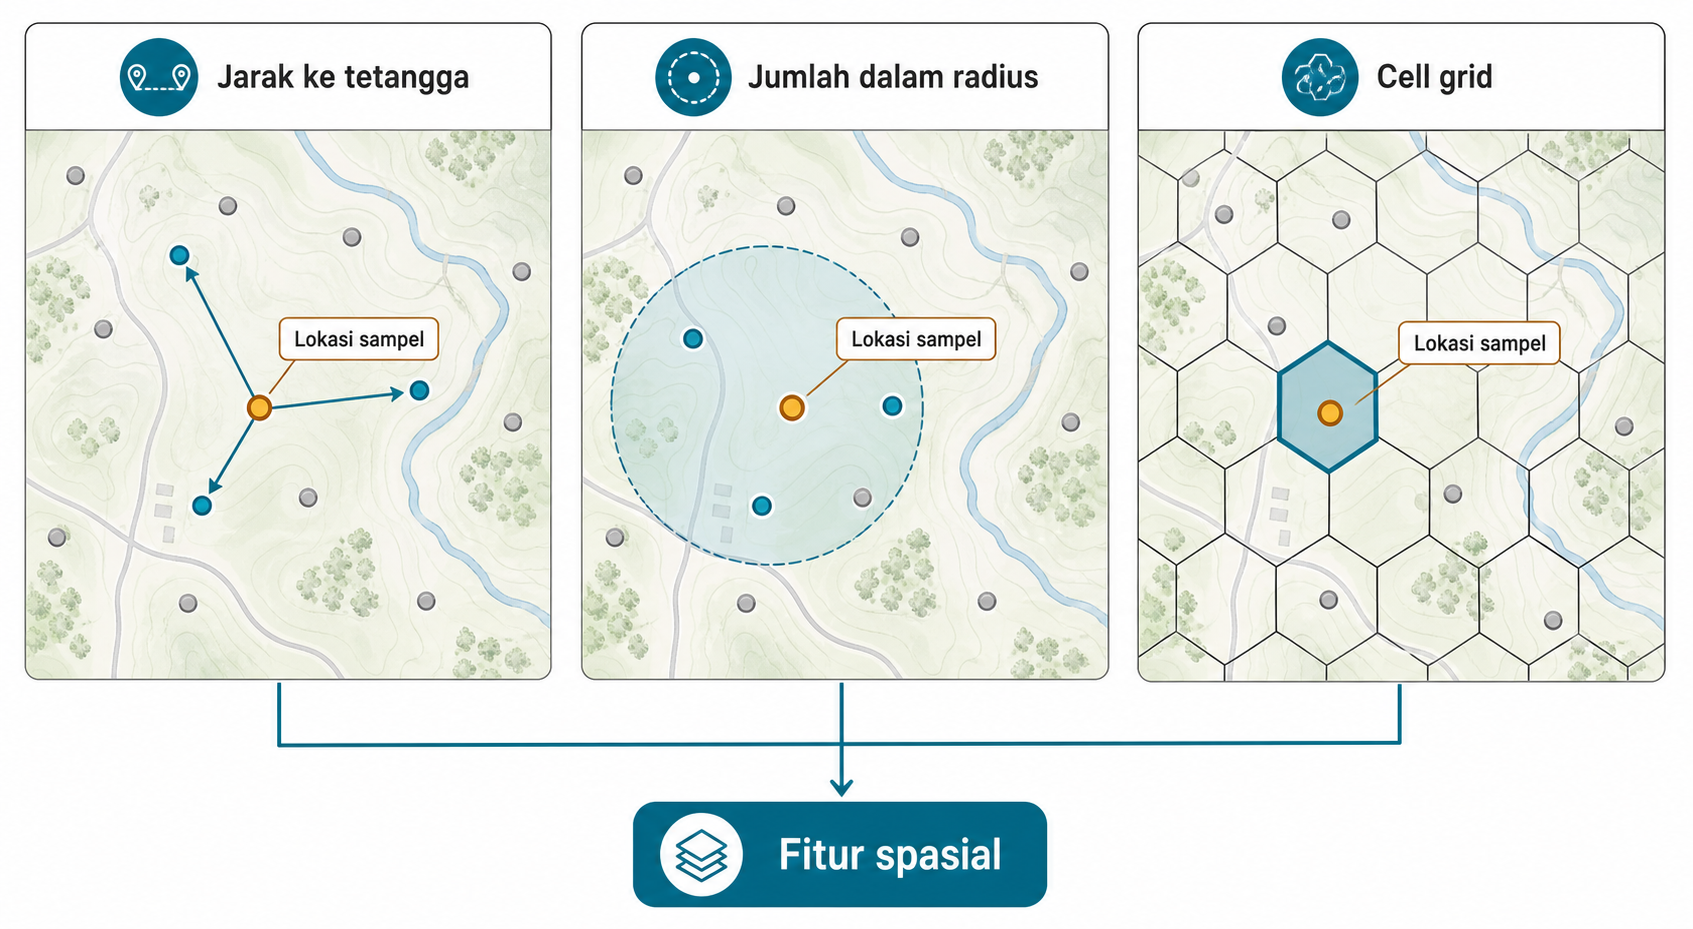
\includegraphics[width=\linewidth,height=0.72\textheight,keepaspectratio]{ch13-fig-1}
\caption{Transformasi Koordinat Mentah Menjadi Fitur Jarak, Radius, dan Indeks Heksagonal}
\label{fig:ch13-fig-1}
\end{figure}

Setelah landasan spasial dikalibrasi, lokasi diterjemahkan dari koordinat absolut menjadi atribut relasional yang prediktif. Praktik ini direpresentasikan melalui dua arsitektur ekstraksi utama:

\begin{enumerate}
\def\labelenumi{\arabic{enumi}.}
\tightlist
\item
  \textbf{Fitur Jarak Absolut (\emph{Distance Features}):} Mengalkulasi metrik spasial menuju titik referensi eksternal. Alih-alih mempelajari koordinat geografis sebuah properti yang kaku, model regresi menerima sinyal ekonomi secara eksplisit melalui atribut ``jarak menuju stasiun kereta terdekat'' atau ``jarak ke pusat bisnis''.
\item
  \textbf{Indeks Spasial Hierarkis:} Memetakan koordinat ke dalam \emph{grid} menggunakan kerangka kerja geospasial modern seperti algoritma H3 yang dikembangkan oleh Uber. H3 memecah permukaan bumi menjadi sel-sel berbentuk heksagonal (\emph{hexagonal hierarchical spatial indexing}). Sistem ini mengonversi titik koordinat acak menjadi atribut pengelompokan (\emph{categorical id}) sel 64-bit yang seragam. Pola indeks ini menyederhanakan perhitungan fitur kedekatan (\emph{proximity}), seperti mengekstraksi metrik ``total kemacetan lalu lintas dalam radius dua sel heksagonal sekeliling titik utama''.
\end{enumerate}

\section{Fitur Ketetanggaan dan Autokorelasi Spasial}\label{fitur-ketetanggaan-dan-autokorelasi-spasial}

Karakteristik mendasar dari data spasial adalah observasi pada suatu lokasi jarang bersifat independen. Prinsip ini dirangkum dalam Hukum Geografi Tobler yang pertama: segala sesuatu saling berhubungan, tetapi sesuatu yang berdekatan memiliki hubungan yang lebih kuat daripada sesuatu yang berjauhan. Ketergantungan terstruktur antar-lokasi ini disebut autokorelasi spasial. Autokorelasi positif berarti area yang letaknya berdekatan cenderung memiliki karakteristik yang serupa.

Model non-spasial, seperti \emph{random forest} atau \emph{gradient boosting}, memproses data dalam format tabular murni. Algoritma ini melihat setiap baris observasi sebagai entitas terisolasi. Jika kita hanya memberikan nilai garis lintang dan bujur sebagai fitur masukan, model akan kesulitan menangkap pola bahwa dua lokasi berdekatan saling memengaruhi. Untuk mengatasi batasan ini, kita perlu secara eksplisit merangkum konteks geografis tersebut ke dalam fitur ketetanggaan numerik yang dapat dipelajari oleh model.

\textbf{Menghitung \emph{Spatial Lag}}

Teknik yang paling lazim digunakan dalam rekayasa fitur spasial adalah \emph{spatial lag}. Representasi ini berwujud nilai rata-rata berbobot dari suatu variabel pada lokasi-lokasi yang menjadi tetangga observasi tersebut.

\[ y_{lag, i} = \sum_{j=1}^{N} w_{ij} y_j \]

Notasi pada persamaan di atas diuraikan sebagai berikut:

\begin{itemize}
\tightlist
\item
  \(y_{lag, i}\) adalah fitur \emph{spatial lag} untuk lokasi \(i\).
\item
  \(w_{ij}\) adalah bobot spasial antara lokasi \(i\) dan tetangganya \(j\). Komponen ini umumnya dinormalisasi per baris (\emph{row-standardized}), sehingga jumlah seluruh bobot untuk satu observasi bernilai satu (\(\sum_j w_{ij} = 1\)).
\item
  \(y_j\) adalah nilai variabel yang diamati pada lokasi tetangga \(j\).
\end{itemize}

Keputusan desain utama terletak pada definisi matriks bobot (\(W\)). Penentuan kandidat ``tetangga'' biasanya menggunakan satu dari tiga skema berikut:

\begin{itemize}
\tightlist
\item
  \textbf{Radius jarak (\emph{distance band}):} Memasukkan semua lokasi yang berada dalam batasan jarak \(r\) kilometer dari titik observasi.
\item
  \textbf{Tetangga terdekat (KNN):} Mengambil sejumlah \(k\) lokasi dengan jarak terpendek, yang menjaga jumlah tetangga tetap konstan terlepas dari kepadatan wilayah.
\item
  \textbf{Kontiguitas:} Menggunakan batas administratif, misalnya menetapkan area dengan kode pos atau kelurahan yang saling bersinggungan sebagai tetangga.
\end{itemize}

\begin{figure}[htbp]\centering
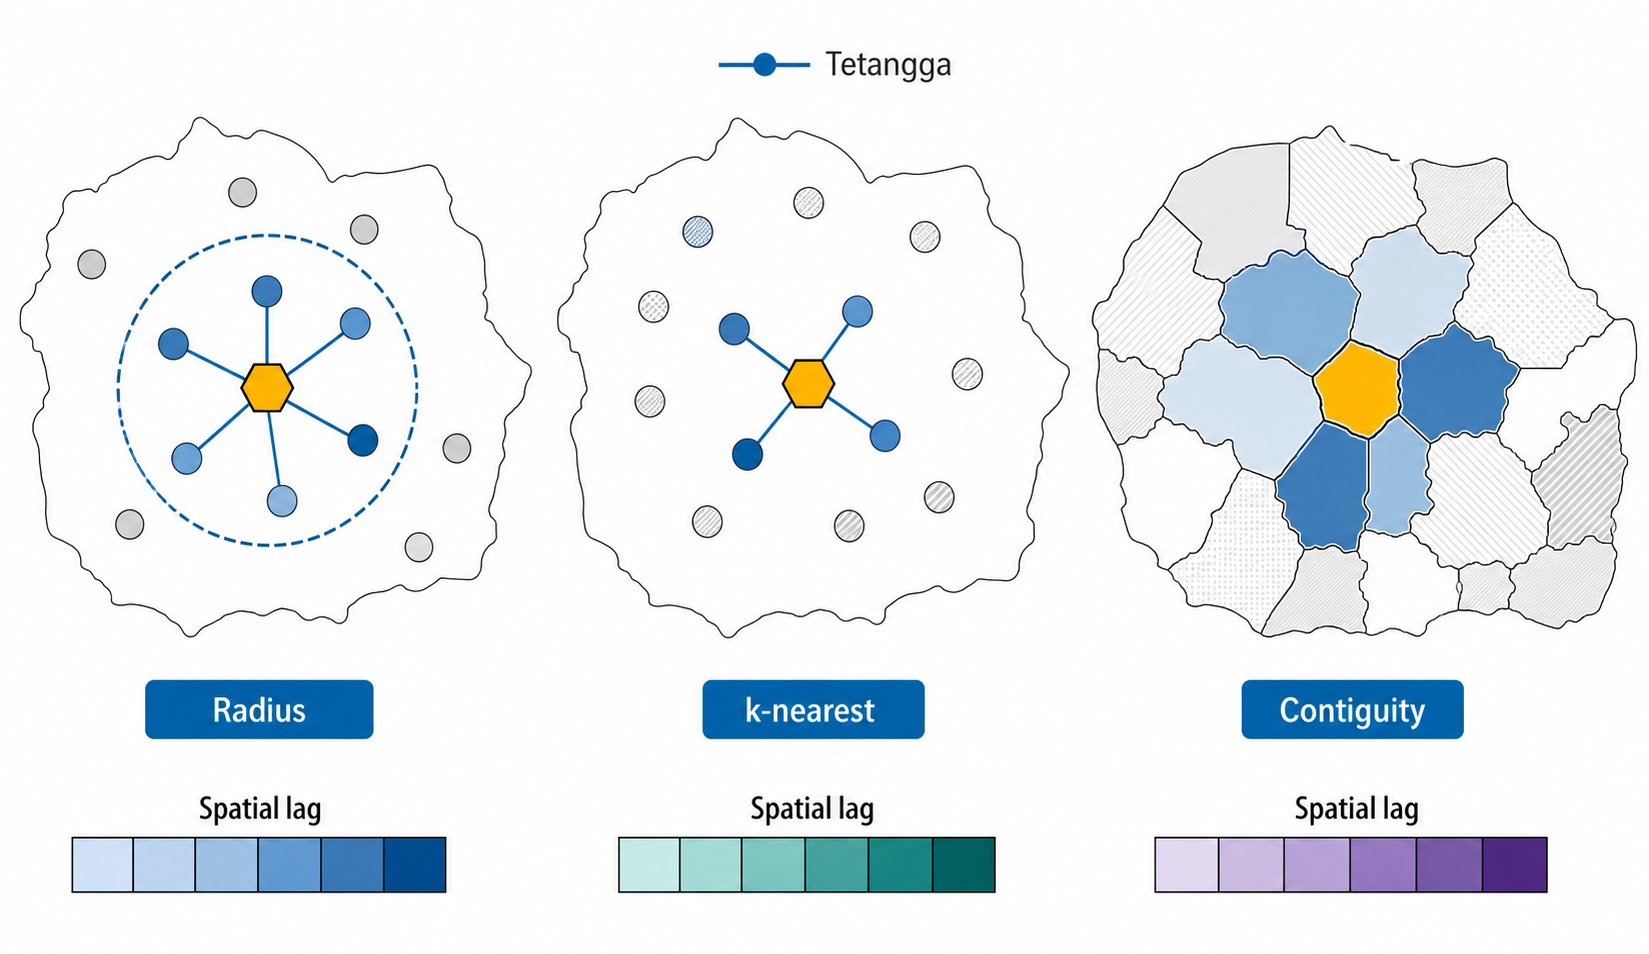
\includegraphics[width=\linewidth,height=0.72\textheight,keepaspectratio]{ch13-fig-2}
\caption{Visualisasi Matriks Bobot Spasial (W) untuk Perhitungan Spatial Lag}
\label{fig:ch13-fig-2}
\end{figure}

\textbf{Indikator Autokorelasi Lokal (LISA)}

Selain \emph{spatial lag} sederhana, pustaka geospasial modern seperti PySAL (\passthrough{\lstinline!esda!}) memungkinkan kita mengekstrak fitur struktural yang lebih kaya. Indikator Autokorelasi Spasial Lokal (LISA), yang dikenal sebagai \emph{Local Moran's I}, mengklasifikasikan setiap observasi ke dalam empat kuadran berdasarkan kemiripannya dengan lingkungan sekitar. Label ini dapat diekstrak menjadi fitur kategorikal:

\begin{itemize}
\tightlist
\item
  \textbf{HH (\emph{High-High}):} Lokasi bernilai tinggi yang dikelilingi tetangga bernilai tinggi (\emph{hot spot}).
\item
  \textbf{LL (\emph{Low-Low}):} Lokasi bernilai rendah di tengah area bernilai rendah (\emph{cold spot}).
\item
  \textbf{HL (\emph{High-Low}):} Pencilan nilai tinggi yang berada di lingkungan bernilai rendah (\emph{diamond}).
\item
  \textbf{LH (\emph{Low-High}):} Pencilan nilai rendah di kawasan bernilai tinggi (\emph{doughnut}).
\end{itemize}

\textbf{Penerapan dan Risiko}

Sebagai contoh, dalam prediksi penjualan toko ritel, model yang hanya dilatih menggunakan atribut internal bangunan akan kehilangan sinyal wilayah. Menambahkan \emph{spatial lag} berupa rata-rata pendapatan penduduk di area sekitar, atau label LISA tentang kepadatan populasi, memungkinkan model menyerap kekuatan daya beli lingkungan tanpa memerlukan representasi spasial dua dimensi yang rumit.

Fitur ketetanggaan memungkinkan model tabular biasa menggunakan konteks ruang secara efisien. Meskipun begitu, ekstraksi fitur ini sangat menuntut praktik pipeline yang benar. Menggunakan nilai target historis dari lokasi sekitar untuk menghitung \emph{lag} sangat rentan memunculkan informasi dari masa depan pada saat prediksi, yang berujung pada terjadinya \emph{leakage} spasial. Risiko spesifik ini menuntut penyesuaian pada strategi pembagian data pada bagian selanjutnya.

\section{\texorpdfstring{\emph{Data Leakage} pada Data Spasial dan \emph{Spatial Cross-Validation}}{Data Leakage pada Data Spasial dan Spatial Cross-Validation}}\label{data-leakage-pada-data-spasial-dan-spatial-cross-validation}

Ketergantungan antar-lokasi dalam data geografis memunculkan kerentanan evaluasi. Data spasial sangat rentan terhadap kebocoran target (\emph{target leakage}) yang merusak validitas metrik performa model.

Akar kebocoran ini adalah autokorelasi spasial, yakni kecenderungan observasi yang saling berdekatan untuk memiliki nilai yang serupa. Fenomena ini sering diukur menggunakan indeks \emph{Moran's I}:

\[ I = \frac{n}{W} \frac{\sum_{i=1}^{n} \sum_{j=1}^{n} w_{ij}(x_i - \bar{x})(x_j - \bar{x})}{\sum_{i=1}^{n} (x_i - \bar{x})^2} \]

Di mana \(n\) adalah jumlah observasi spasial, \(x_i\) dan \(x_j\) adalah nilai fitur pada lokasi \(i\) dan \(j\), \(\bar{x}\) adalah rata-rata fitur, \(w_{ij}\) melambangkan bobot spasial antara lokasi \(i\) dan \(j\) (skor ketetanggaan), serta \(W\) adalah jumlah total bobot spasial. Nilai \(I\) yang tinggi dan positif menunjukkan kuatnya autokorelasi, yang berarti informasi target dapat mengalir melintasi batas observasi secara tak kasatmata.

\subsection{Kegagalan Validasi Silang Acak}\label{kegagalan-validasi-silang-acak}

Pemisahan data secara acak (\emph{random k-fold cross-validation}) menghasilkan partisi latih dan uji yang tersebar menyerupai taburan garam dan merica (\emph{salt and pepper}) di atas peta. Metode ini gagal pada data spasial akibat tiga masalah utama:

\begin{itemize}
\tightlist
\item
  \textbf{Kontaminasi Jarak Dekat:} Titik data uji sering kali berbatasan langsung dengan titik data latih.
\item
  \textbf{Metrik Akurasi Semu:} Model mencetak akurasi tinggi akibat menghafal nilai dari titik tetangga terdekatnya yang bocor ke set latih, tanpa mempelajari pola lingkungan secara umum.
\item
  \textbf{Penurunan Performa:} Saat model diterapkan pada lokasi baru, kinerjanya turun drastis karena kehilangan akses ke sinyal tetangga tersebut.
\end{itemize}

\subsection{\texorpdfstring{\emph{Spatial Cross-Validation} dan Zona Penyangga}{Spatial Cross-Validation dan Zona Penyangga}}\label{spatial-cross-validation-dan-zona-penyangga}

Penerapan \emph{praktik pipeline yang benar} mengharuskan model dievaluasi menggunakan \emph{spatial cross-validation}. Metode ini mencegah kebocoran dengan memblokir observasi berdekatan agar tidak terpisah ke dua set yang berbeda.

Proses evaluasi spasial beroperasi melalui dua mekanisme pembatasan:

\begin{enumerate}
\def\labelenumi{\arabic{enumi}.}
\tightlist
\item
  \textbf{Pemisahan Berbasis Blok:} Peta dibagi menjadi beberapa wilayah atau blok besar. Seluruh observasi dalam satu blok dialokasikan sebagai data latih, dan blok lainnya sepenuhnya difungsikan sebagai data uji.
\item
  \textbf{Zona Penyangga (\emph{Buffer}):} Jarak aman atau zona mati (\emph{dead zone}) diterapkan di sekitar batas blok uji. Titik latih yang masuk ke dalam rentang zona ini dihapus selama proses pelatihan guna memotong kebocoran informasi jarak dekat.
\end{enumerate}

\begin{figure}[htbp]\centering
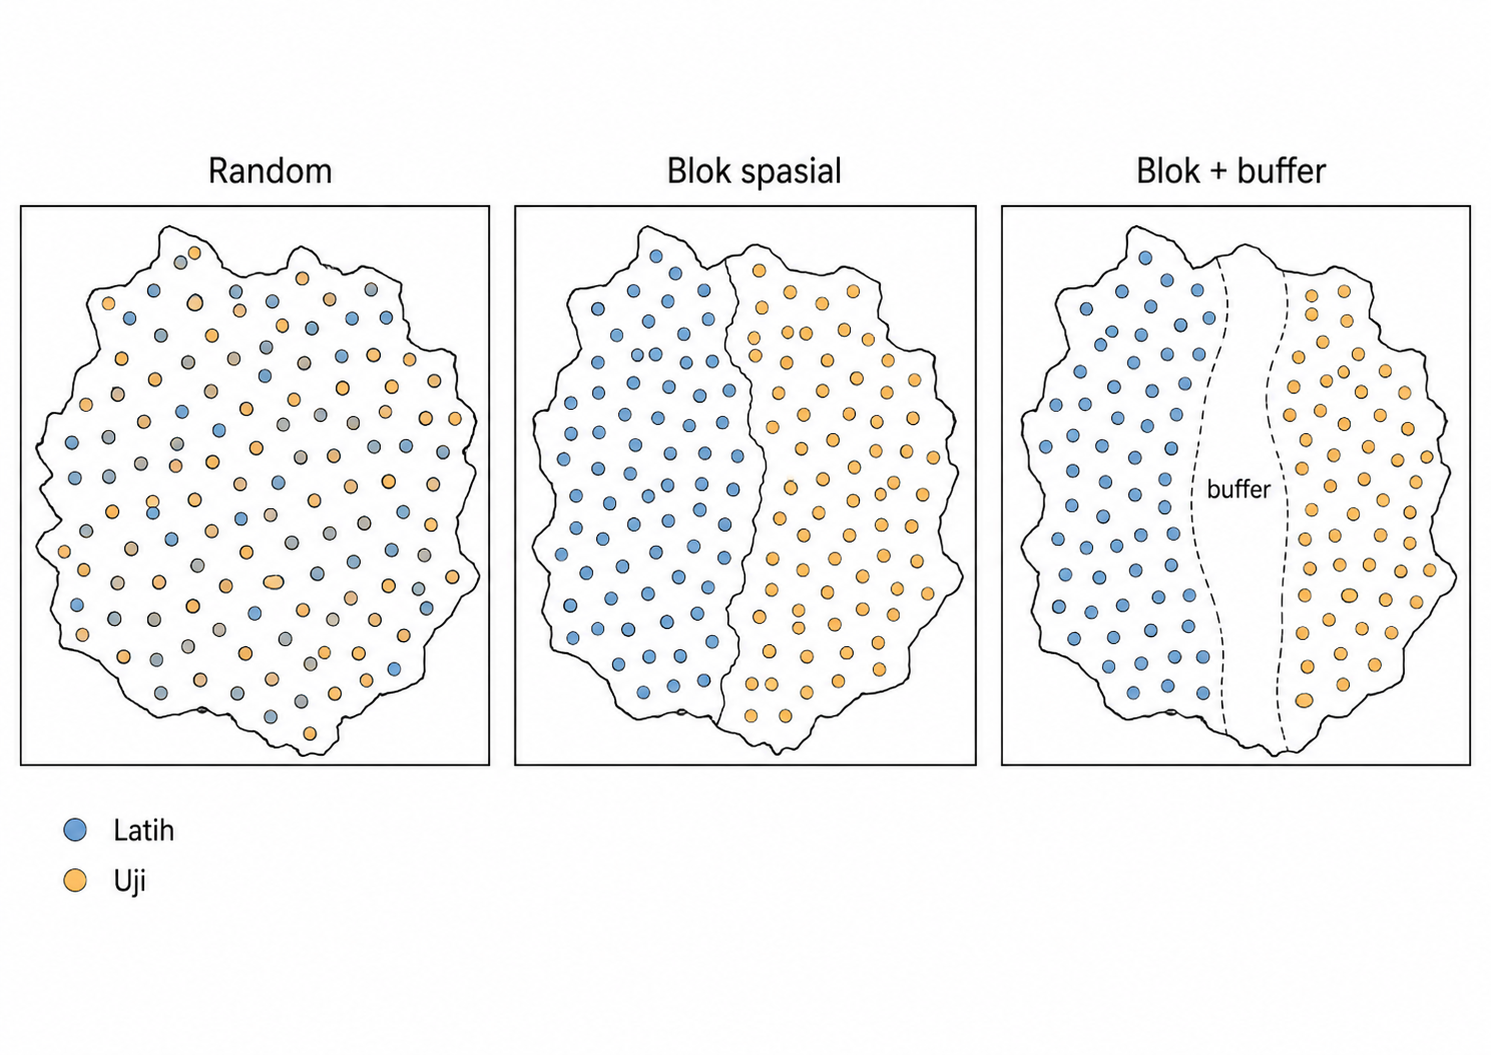
\includegraphics[width=\linewidth,height=0.72\textheight,keepaspectratio]{ch13-fig-3}
\caption{Pemisahan Acak vs Pemisahan Blok Spasial dengan Zona Penyangga (Buffer Zone)}
\label{fig:ch13-fig-3}
\end{figure}

Kasus prediksi deforestasi dari citra satelit memperlihatkan dampak metode ini dengan jelas. Karakteristik tutupan lahan sebuah piksel satelit memiliki korelasi kuat dengan piksel di sekelilingnya. Jika dipisahkan secara acak, model dapat mendeteksi status tetangga piksel uji tanpa mengekstrak ciri visual hutan yang gundul. Sebaliknya, pemisahan blok spasial memaksa model mengidentifikasi indikator lingkungan yang objektif sehingga sistem siap diterapkan pada wilayah yang belum pernah direkam.

\section{Data Graf: Derajat, Sentralitas, dan Fitur Klaster}\label{data-graf-derajat-sentralitas-dan-fitur-klaster}

Data tabular standar memperlakukan setiap baris observasi secara independen. Data graf beroperasi dengan asumsi sebaliknya, di mana makna sebuah observasi sangat bergantung pada interaksinya dengan entitas lain. Dalam struktur data ini, entitas direpresentasikan sebagai simpul dan interaksi antar entitas sebagai sisi.

Model \emph{machine learning} konvensional seperti regresi logistik atau \emph{random forest} tidak dapat menerima input berupa topologi jaringan mentah. Model tersebut mensyaratkan struktur data berbentuk matriks datar yang berisi vektor numerik berdimensi tetap. Oleh karena itu, properti relasional jaringan harus diekstrak menjadi sekumpulan fitur struktural. Proses mengubah relasi menjadi kolom numerik ini adalah bentuk representasi yang dirancang manusia, yang bertujuan merangkum konteks lokal dan posisi global setiap simpul ke dalam \emph{pipeline} prediksi tabular biasa.

Pengekstraksian fitur topologi pada graf umumnya memanfaatkan tiga kategori metrik:

\begin{itemize}
\tightlist
\item
  \textbf{Derajat (\emph{Degree}):} Menghitung jumlah sisi yang terhubung langsung ke sebuah simpul. Pada graf berarah, perhitungan dipecah menjadi \emph{in-degree} (indikator daya tarik atau popularitas) dan \emph{out-degree} (indikator tingkat aktivitas komunikasi). Untuk memfasilitasi perbandingan ukuran antar jaringan, jumlah sisi mutlak ini diubah menjadi sentralitas derajat (\emph{degree centrality}):
\end{itemize}

\[ C_d(v) = \frac{\text{deg}(v)}{N - 1} \]

Di mana \(C_d(v)\) adalah nilai sentralitas derajat untuk simpul \(v\), \(\text{deg}(v)\) mewakili jumlah koneksi langsung yang dimiliki \(v\), dan \(N\) adalah total jumlah simpul di dalam graf. Pembagi \(N-1\) merupakan jumlah koneksi maksimal yang mungkin dimiliki sebuah simpul ke seluruh simpul lainnya.

\begin{itemize}
\item
  \textbf{Sentralitas (\emph{Centrality}):} Mengukur nilai strategis sebuah simpul berdasarkan posisinya di dalam arsitektur global graf. Sentralitas mengevaluasi kekuatan struktural yang tidak dapat ditangkap hanya dengan menghitung jumlah koneksi langsung.
\item
  \textbf{PageRank:} Menilai tingkat otoritas simpul secara rekursif. Sebuah simpul mendapat skor tinggi jika ia menerima sisi dari simpul-simpul lain yang juga berstatus penting.
\item
  \textbf{Betweenness:} Mengukur seberapa penting peran sebuah simpul sebagai titik jembatan. Fitur ini menghitung proporsi jalur terpendek (\emph{shortest path}) antar semua pasangan simpul yang melewati simpul target. Simpul dengan \emph{betweenness} tinggi memegang kendali atas aliran informasi antar kelompok meskipun tidak memiliki banyak koneksi langsung.
\item
  \textbf{Koefisien Klaster (\emph{Clustering Coefficient}):} Menilai kepadatan interaksi lokal. Metrik ini menghitung proporsi tetangga dari sebuah target yang juga saling terhubung satu sama lain. Nilai koefisien tinggi menandakan kehadiran simpul di dalam suatu komunitas yang berikatan erat (\emph{clique}).
\end{itemize}

\begin{figure}[htbp]\centering
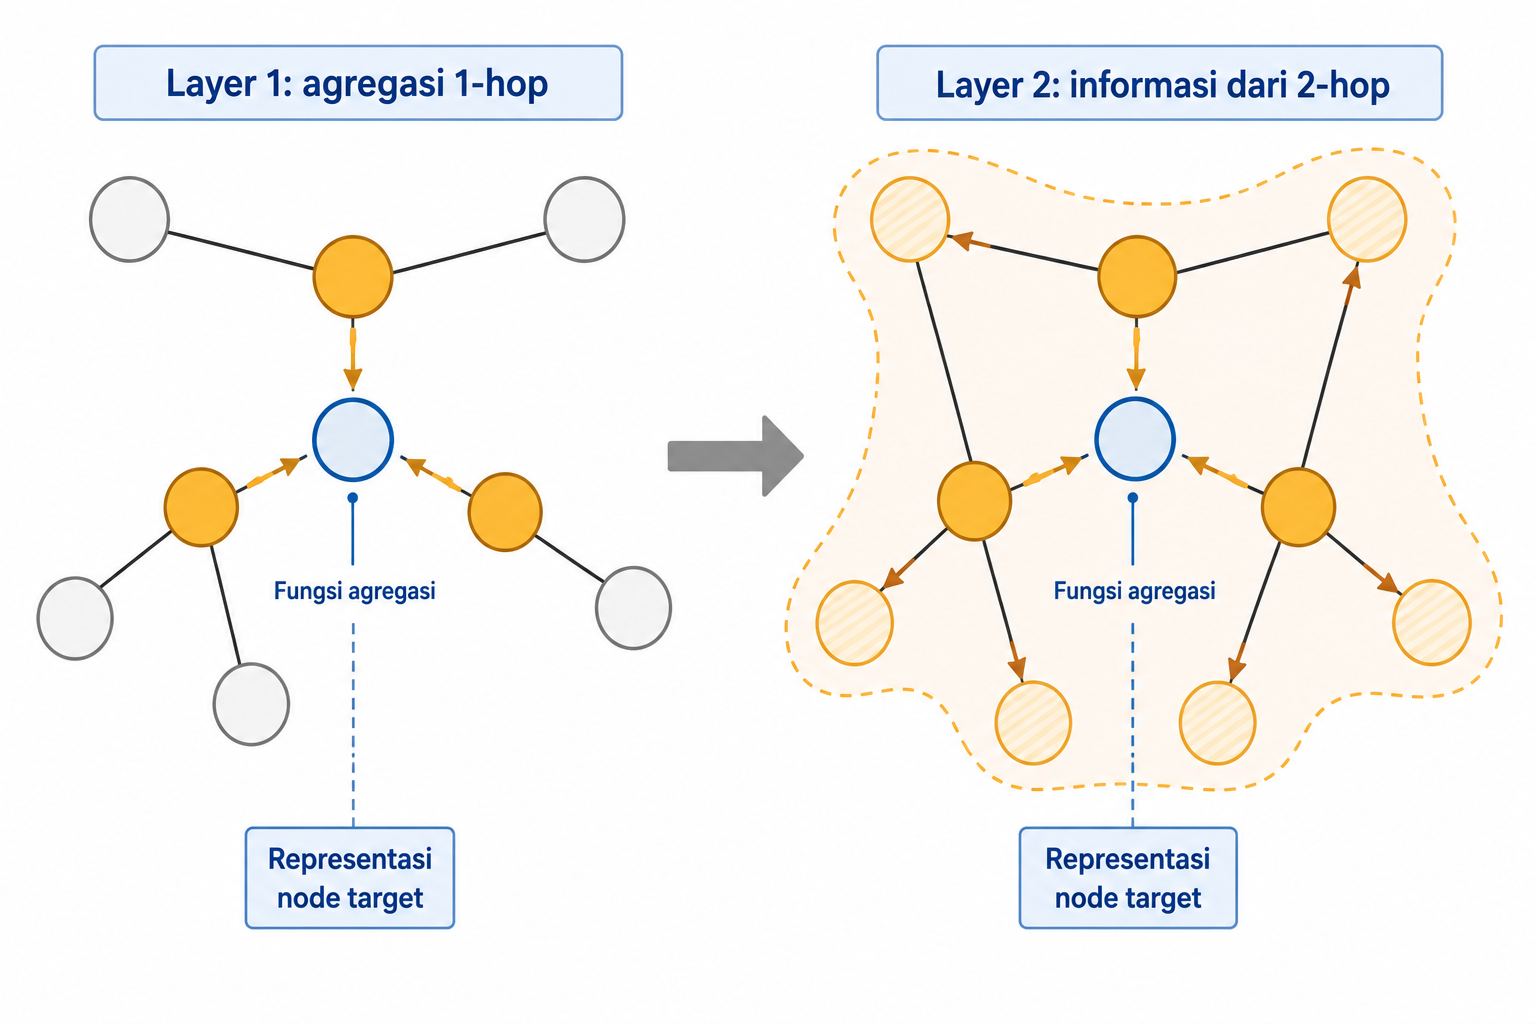
\includegraphics[width=\linewidth,height=0.72\textheight,keepaspectratio]{ch13-fig-4}
\caption{Pengukuran Sentralitas (Degree vs Betweenness) pada Jaringan Graf}
\label{fig:ch13-fig-4}
\end{figure}

Pustaka numerik seperti NetworkX menyediakan fungsi kalkulasi siap pakai untuk merangkum keseluruhan metrik di atas. Validitas representasi struktural ini terlihat jelas pada kasus klasifikasi penipuan di jaringan sosial. Akun bot secara tipikal memiliki angka \emph{out-degree} masif karena mengikuti ribuan akun secara agresif, tetapi menahan \emph{in-degree} di angka nol. Apabila ditambah dengan koefisien klaster yang bernilai nol, matriks hasil transformasi ini secara eksplisit mengkategorikan isolasi struktural sebuah observasi. Transformasi awal ini mematangkan data graf mentah menjadi input tabular standar sebagai jembatan yang diperlukan sebelum beralih menggunakan representasi yang dipelajari mesin.

\section{Agregasi Ketetanggaan dan Fitur Berbasis Jalur}\label{agregasi-ketetanggaan-dan-fitur-berbasis-jalur}

Metrik derajat (\emph{degree}) menangkap tingkat aktivitas dasar sebuah simpul, tetapi tidak mendeskripsikan konteks interaksi di sekelilingnya. Agregasi ketetanggaan merangkum atribut dari seluruh simpul yang terhubung langsung dengan sebuah simpul target. Pendekatan ini menyerupai fitur \emph{spatial lag} pada data geospasial. Kedekatan pada graf diukur melalui jarak topologi, berbeda dengan jarak fisik pada data koordinat.

Fungsi agregasi matematika menormalkan variabilitas ukuran lingkungan graf. Sebuah simpul bisa memiliki satu tetangga sementara simpul lain memiliki ratusan tetangga. Fungsi agregasi menyusutkan lingkungan yang heterogen ini menjadi dimensi fitur yang tetap, sehingga model prediktif menerima jumlah kolom masukan yang seragam. Beberapa pendekatan agregasi umum meliputi:

\begin{itemize}
\tightlist
\item
  \textbf{Rata-rata (\emph{Mean}):} Menghitung nilai tengah dari atribut tetangga.
\item
  \textbf{Jumlah (\emph{Sum}):} Mengakumulasi total atribut tetangga.
\item
  \textbf{Nilai Maksimum (\emph{Max}):} Menangkap sinyal terkuat di sekitar simpul target.
\end{itemize}

Sebagai contoh, model deteksi kelayakan kredit mengevaluasi pendapatan target sekaligus menghitung rata-rata skor kredit dari seluruh individu dalam lingkaran transaksinya. Sinyal yang diekstrak dari lingkungan ini memberikan daya prediksi tambahan melebihi data individu tunggal.

Formulasi dasar untuk agregasi nilai rata-rata dapat dituliskan sebagai berikut:

\[ h_v = \frac{1}{|\mathcal{N}(v)|} \sum_{u \in \mathcal{N}(v)} x_u \]

Di mana \(h_v\) adalah fitur agregasi untuk simpul target \(v\), \(\mathcal{N}(v)\) merupakan himpunan simpul tetangga yang terhubung langsung dengan \(v\), \(|\mathcal{N}(v)|\) adalah jumlah tetangga tersebut, dan \(x_u\) mewakili vektor atribut dari simpul tetangga \(u\).

\begin{figure}[htbp]\centering
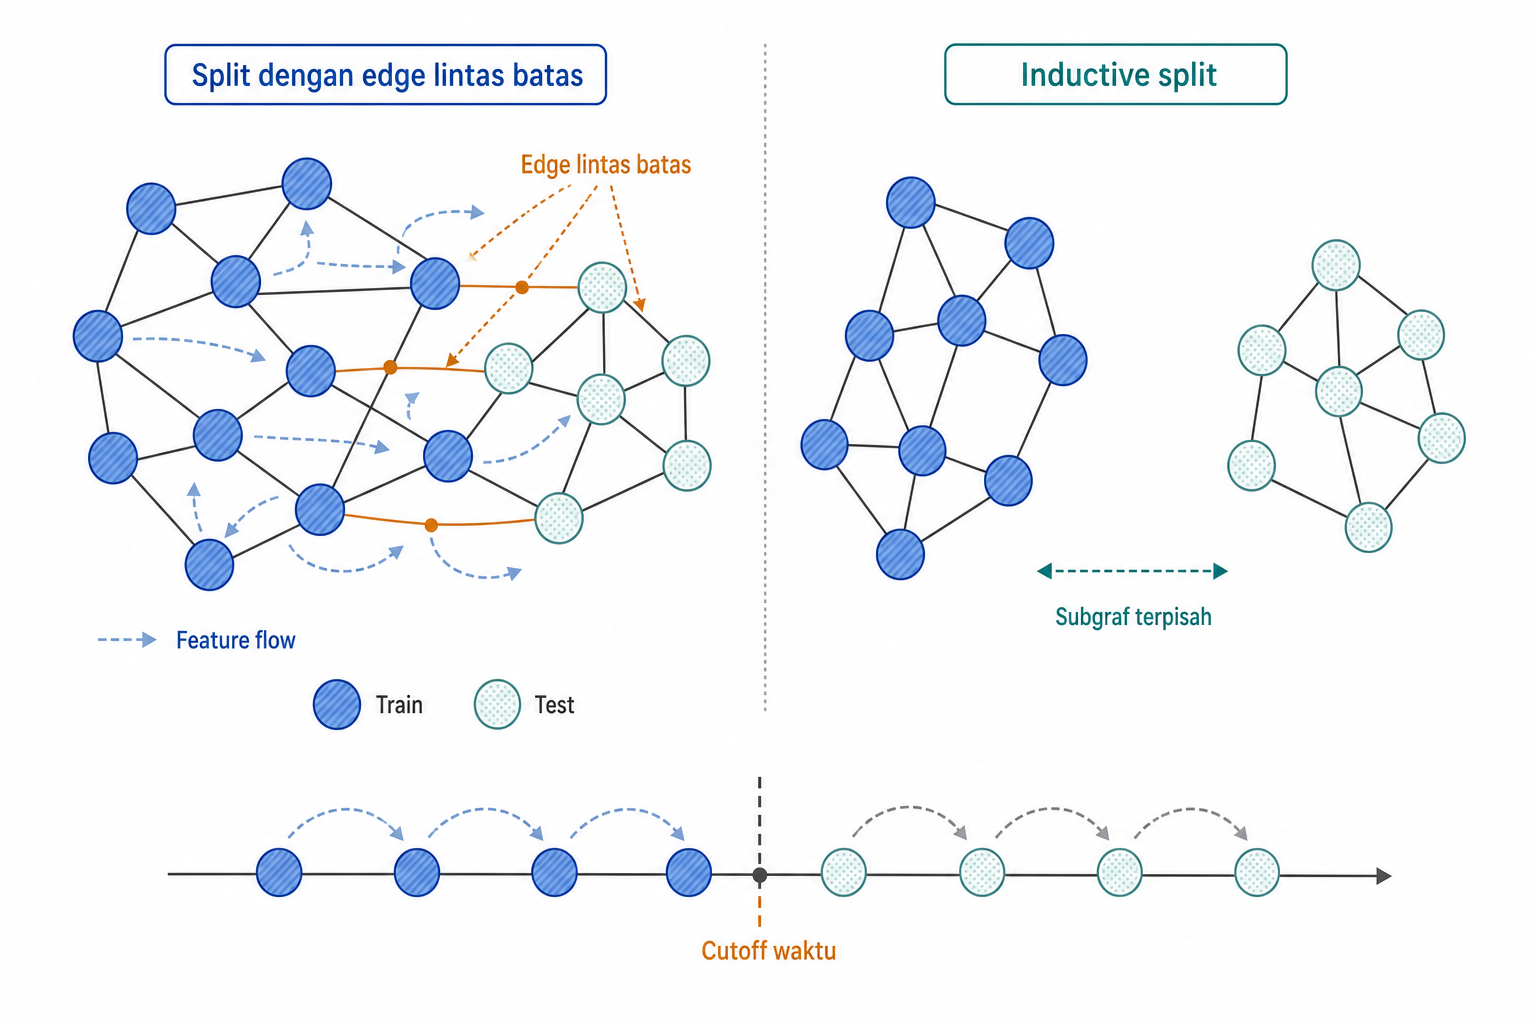
\includegraphics[width=\linewidth,height=0.72\textheight,keepaspectratio]{ch13-fig-5}
\caption{Proses Agregasi Atribut dari Simpul Tetangga dan Ekstraksi Jalur Struktural}
\label{fig:ch13-fig-5}
\end{figure}

Topologi graf juga memfasilitasi ekstraksi fitur berbasis jalur yang melacak rute relasional antar entitas. Fitur ini jamak diaplikasikan pada tugas prediksi tautan (\emph{link prediction}), seperti pada sistem rekomendasi. Metrik numerik yang diturunkan dari struktur jalur meliputi:

\begin{itemize}
\tightlist
\item
  \textbf{Jarak terpendek (\emph{Shortest path}):} Jumlah langkah minimum yang dibutuhkan untuk menghubungkan dua simpul berbeda.
\item
  \textbf{Tetangga bersama (\emph{Common neighbors}):} Total persimpangan simpul yang terhubung ke kedua entitas secara bersamaan.
\item
  \textbf{Indeks Adamic-Adar:} Pembobotan dari metode \emph{common neighbors} yang memberi nilai lebih tinggi pada tetangga bersinggungan dengan derajat rendah. Asumsinya, koneksi spesifik membawa sinyal kedekatan yang lebih kuat dibandingkan koneksi melalui simpul hub populer.
\end{itemize}

Pada sistem rekomendasi, ketersediaan banyak jalur pendek antara profil pengguna dan produk menunjukkan probabilitas interaksi yang tinggi.

Seluruh metode agregasi ketetanggaan dan metrik jarak mendatarkan struktur jaringan yang kompleks ke dalam matriks fitur konvensional. Transformasi lokal ini membuat karakteristik graf dapat diproses oleh algoritma \emph{machine learning} standar. Praktik merangkum atribut tetangga secara manual ini menjadi jembatan menuju arsitektur GraphSAGE dan \emph{Graph Neural Networks} (GNN), yang mengubah agregasi statis ini menjadi mekanisme pertukaran pesan yang dipelajari mesin secara dinamis.

\section{Embedding Simpul: Node2Vec dan Representasi Laten}\label{embedding-simpul-node2vec-dan-representasi-laten}

Fitur graf tradisional seperti derajat, sentralitas, dan agregasi jalur membutuhkan perancangan metrik secara eksplisit. Pendekatan ini merupakan wujud representasi yang dirancang manusia, yang sangat bergantung pada intuisi dan kepakaran domain. Sebagai alternatif, kita menggunakan representasi yang dipelajari mesin melalui \emph{node embedding}. Dalam metode ini, setiap simpul diproyeksikan ke vektor numerik padat (\emph{dense vector}) di ruang laten. Kedekatan geometris antarvektor di ruang ini menangkap kemiripan struktur dan peran antar-simpul.

Salah satu metode yang paling mapan untuk mempelajari representasi ini adalah \emph{Node2Vec}. Algoritma ini mengembangkan metode \emph{DeepWalk}, yang mengadaptasi \emph{Word2Vec} dari pemrosesan bahasa alami untuk menangani data graf. Karena graf tidak memiliki kalimat linear, \emph{Node2Vec} menyimulasikan deretan simpul secara buatan melalui pelompatan acak (\emph{random walk}). \emph{DeepWalk} berpindah simpul dengan probabilitas seragam. Sementara itu, \emph{Node2Vec} menggunakan pelompatan acak berbias (\emph{biased random walk}) untuk mengendalikan arah penjelajahan. Probabilitas transisi diformulasikan sebagai:

\[P(c_i = x \mid c_{i-1} = v) = \frac{\pi_{vx}}{Z}\]

Di mana \(c_i\) adalah simpul pada langkah ke-\(i\) dalam lintasan, \(\pi_{vx}\) adalah probabilitas transisi tidak ternormalisasi dari simpul \(v\) ke tetangganya \(x\), dan \(Z\) merupakan konstanta normalisasi.

Nilai bias \(\pi_{vx}\) dikendalikan oleh dua parameter utama:

\begin{itemize}
\tightlist
\item
  \textbf{Parameter pengembalian (\(p\)):} Mengendalikan probabilitas untuk segera kembali ke simpul sebelumnya. Nilai \(p\) yang rendah mendorong eksplorasi lokal (\emph{Breadth-First Search} atau BFS), yang ideal untuk menangkap kedekatan komunitas atau homofili (\emph{homophily}).
\item
  \textbf{Parameter masuk-keluar (\(q\)):} Mengendalikan probabilitas untuk menjelajah menjauhi simpul asal. Nilai \(q\) yang rendah mendukung eksplorasi ke area yang lebih jauh (\emph{Depth-First Search} atau DFS), yang bermanfaat untuk menangkap kesetaraan struktural (\emph{structural equivalence}), seperti menemukan simpul-simpul yang berperan sebagai jembatan lintas komunitas.
\end{itemize}

\begin{figure}[htbp]\centering
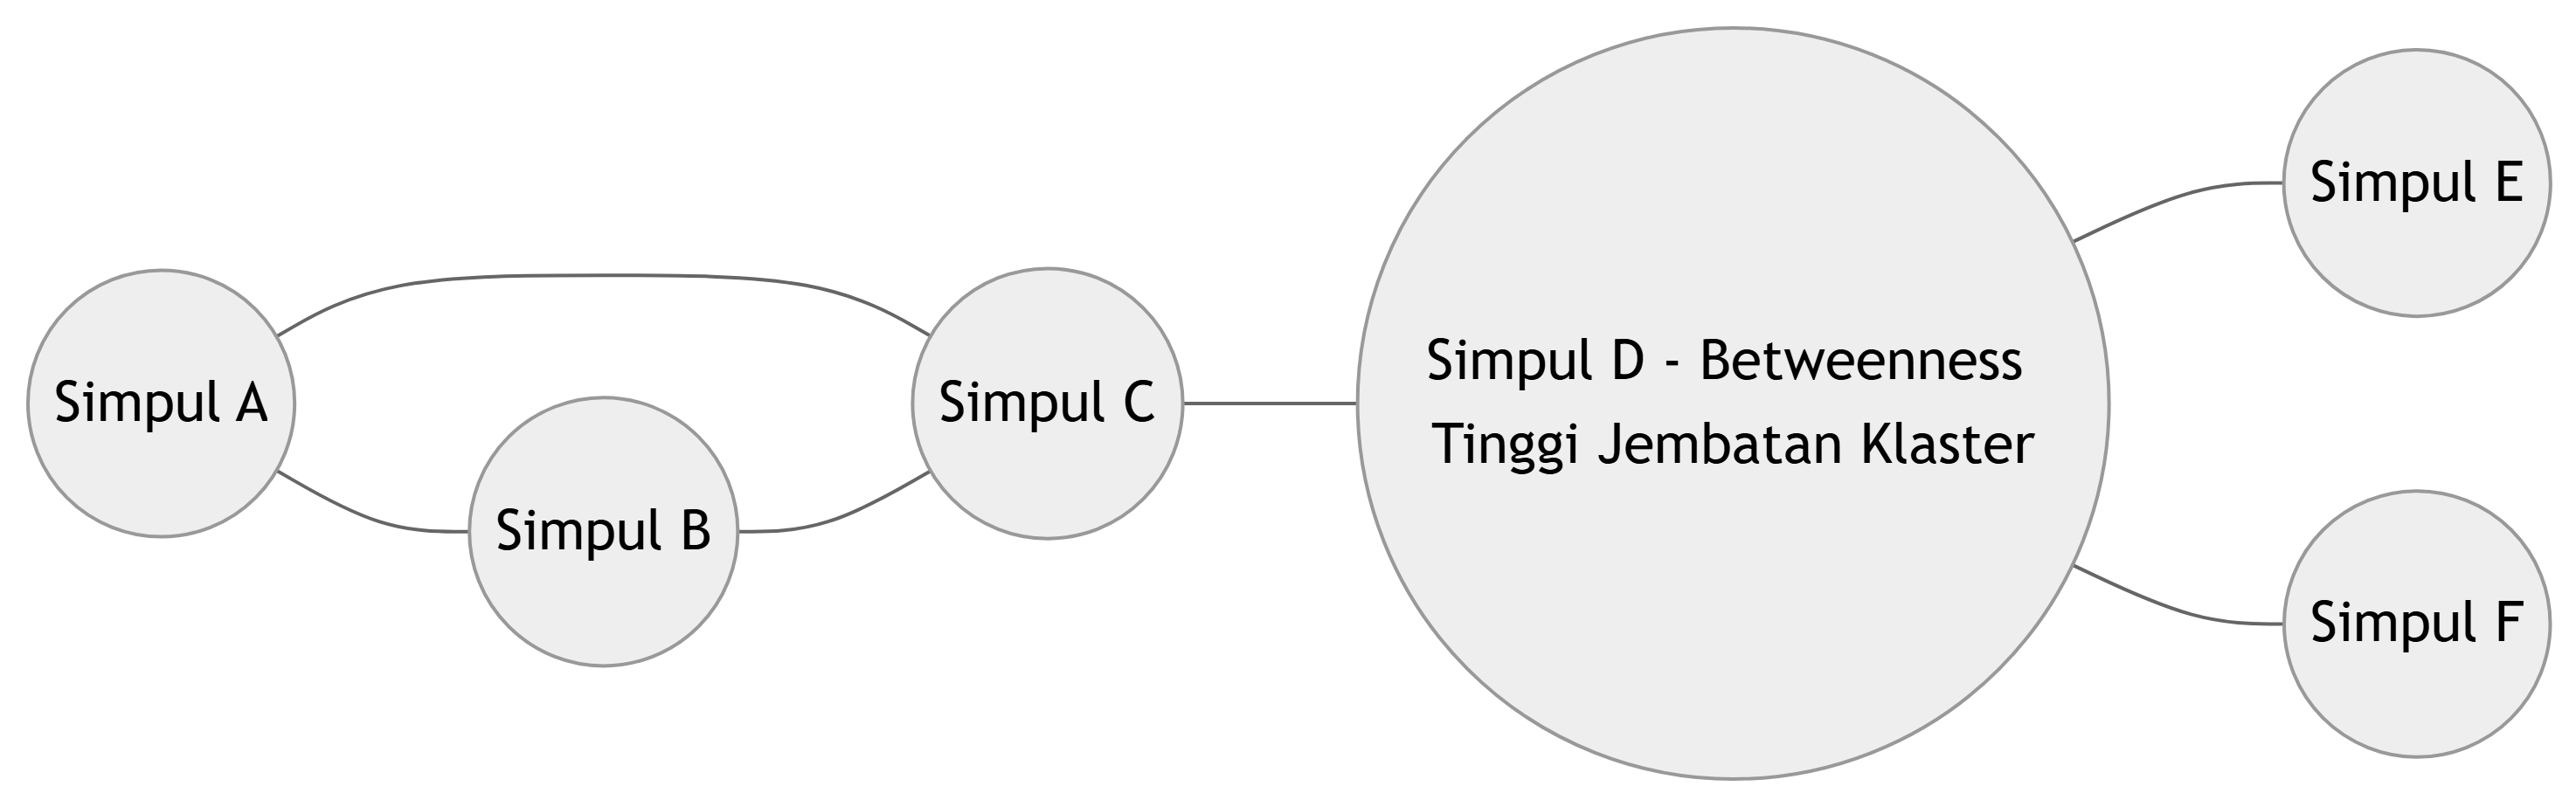
\includegraphics[width=\linewidth,height=0.72\textheight,keepaspectratio]{ch13-fig-6}
\caption{Skema Random Walk (Node2Vec) dengan Parameter p dan q}
\label{fig:ch13-fig-6}
\end{figure}

Urutan simpul hasil pelompatan ini diperlakukan layaknya kalimat. \emph{Node2Vec} menerapkan arsitektur \emph{Word2Vec} tipe \emph{Skip-gram} untuk memaksimalkan probabilitas munculnya simpul-simpul tetangga di sekitar simpul target:

\[\max_{\mathbf{z}} \sum_{u \in V} \log P(\mathcal{N}_S(u) \mid \mathbf{z}_u)\]

Di mana \(\mathbf{z}_u\) adalah vektor laten dari simpul \(u\), \(V\) adalah himpunan seluruh simpul, dan \(\mathcal{N}_S(u)\) adalah kelompok tetangga simpul \(u\) yang dihasilkan dari strategi pelompatan (\emph{random walk}). Probabilitas ini dimodelkan menggunakan \emph{dot product} antarvektor. Simpul yang sering muncul bersama pada lintasan yang sama akan memiliki nilai \emph{dot product} tinggi, sehingga posisinya berakhir saling berdekatan.

Sebagai contoh, jika diterapkan pada jaringan kutipan akademik, model akan menghasilkan vektor laten yang menangkap posisi struktural jurnal tersebut. Vektor ini langsung menjadi fitur masukan untuk regresi logistik tanpa perhitungan fitur manual.

Namun, metode ini memiliki dua batasan mendasar:

\begin{enumerate}
\def\labelenumi{\arabic{enumi}.}
\tightlist
\item
  \textbf{Mengabaikan atribut simpul:} Vektor dilatih murni dari topologi graf. \emph{Node2Vec} tidak dapat memanfaatkan fitur bawaan simpul, seperti data teks abstrak pada makalah akademik.
\item
  \textbf{Bersifat \emph{transductive}:} Metode ini membangun tabel pencarian (\emph{lookup table}) statis dan tidak dapat menghasilkan \emph{embedding} untuk simpul baru yang muncul setelah fase pelatihan selesai.
\end{enumerate}

Kedua batasan ini mendorong transisi ke arsitektur jaringan saraf graf yang mampu merampatkan fungsi agregasi ke simpul tak terlihat.

\section{Graph Neural Networks (GNN) sebagai Ekstraktor Fitur}\label{graph-neural-networks-gnn-sebagai-ekstraktor-fitur}

Teknik \emph{embedding} berbasis pelompatan acak (\emph{random walk}) seperti \emph{Node2Vec} sangat baik dalam menangkap struktur graf, tetapi mengabaikan atribut asli yang melekat pada simpul. Dalam jejaring sosial, teknik ini dapat memetakan pola pertemanan antarindividu, namun akan mengabaikan informasi pendukung seperti usia, pekerjaan, atau minat pengguna. \emph{Graph Neural Network} (GNN) hadir untuk menyelesaikan masalah ini dengan memadukan struktur jaringan dan atribut masing-masing simpul secara bersamaan. Pendekatan ini menghasilkan representasi yang dipelajari mesin yang jauh lebih kaya.

GNN bekerja layaknya versi terotomatisasi dari kalkulasi lingkungan ketetanggaan. Daripada merancang fitur secara manual melalui penghitungan statistik, GNN menggunakan mekanisme \emph{message passing} agar jaringan dapat mempelajari sendiri cara terbaik untuk merangkum dan menyerap informasi di sekitarnya.

Secara matematis, fungsi agregasi pada lapisan \emph{Graph Convolutional Network} (GCN) dirumuskan sebagai berikut:

\[ \mathbf{h}_v^{(k)} = \sigma \left( \mathbf{W}^{(k)} \sum_{u \in \mathcal{N}(v)} \frac{\mathbf{h}_u^{(k-1)}}{|\mathcal{N}(v)|} + \mathbf{B}^{(k)} \mathbf{h}_v^{(k-1)} \right) \]

Penjelasan notasi di atas:

\begin{itemize}
\tightlist
\item
  \(\mathbf{h}_v^{(k)}\) mewakili vektor representasi simpul target \(v\) pada lapisan ke-\(k\).
\item
  \(\mathbf{h}_u^{(k-1)}\) merupakan vektor representasi dari simpul tetangga \(u\) yang diproses pada lapisan sebelumnya.
\item
  \(\mathcal{N}(v)\) menunjukkan himpunan semua simpul yang bertetangga langsung dengan \(v\).
\item
  \(\mathbf{W}^{(k)}\) dan \(\mathbf{B}^{(k)}\) bertindak sebagai matriks bobot yang diperbarui iteratif selama proses pelatihan model.
\item
  \(\sigma\) mewakili fungsi aktivasi non-linear.
\end{itemize}

Persamaan tersebut menjelaskan bahwa simpul \(v\) mengumpulkan seluruh nilai representasi dari para tetangganya, mengambil nilai rata-rata, lalu memodifikasinya menggunakan matriks bobot \(\mathbf{W}^{(k)}\). Di saat yang sama, identitas atau informasi dari simpul itu sendiri tetap dipertahankan dengan menyertakan perhitungan fungsi matriks bobot \(\mathbf{B}^{(k)}\).

\begin{figure}[htbp]\centering
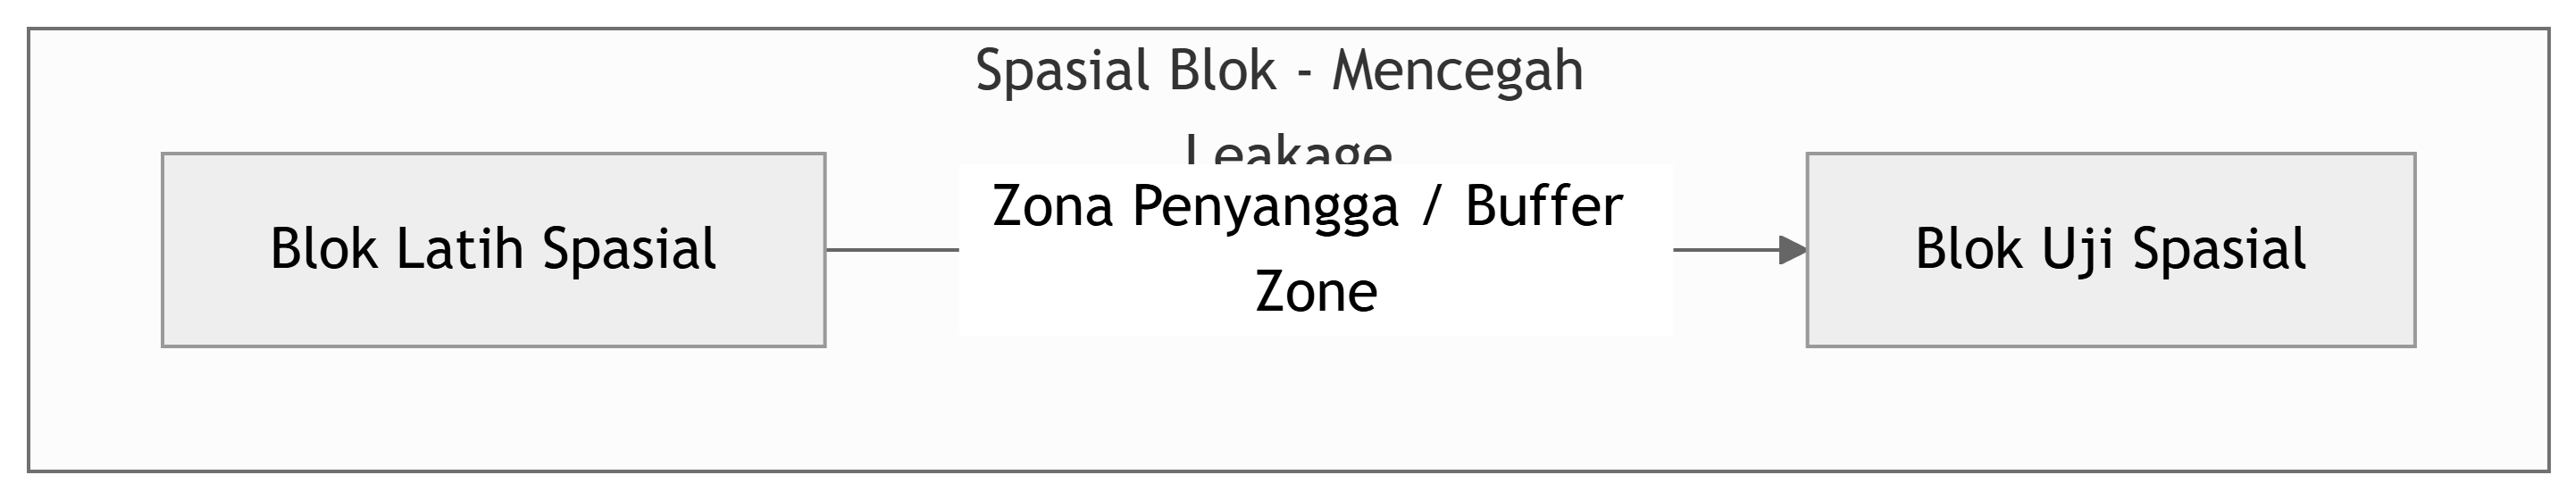
\includegraphics[width=\linewidth,height=0.72\textheight,keepaspectratio]{ch13-fig-7}
\caption{Pesan Agregasi GNN}
\label{fig:ch13-fig-7}
\end{figure}

Judul: Mekanisme message passing pada Graph Neural Network.
Tipe: skema
Tampilkan: Ilustrasi simpul target yang menerima pesan berupa vektor fitur dari simpul-simpul tetangganya, menggabungkannya, dan memprosesnya menggunakan jaringan saraf untuk memperbarui representasinya sendiri.
Sumber data: -

Melalui proses penghitungan bertingkat ke dalam, area konteks yang mampu dipelajari model akan semakin melebar:

\begin{enumerate}
\def\labelenumi{\arabic{enumi}.}
\tightlist
\item
  \textbf{Lapisan Pertama:} Jaringan mulai menyerap atribut informasi dari simpul yang berbatasan secara langsung (tetangga 1-hop).
\item
  \textbf{Lapisan Kedua:} Jaringan dapat mengumpulkan konteks yang berasal dari tetangga para tetangganya (area 2-hop).
\item
  \textbf{Vektor Keluaran:} Representasi numerik padat akan dihasilkan pada bagian paling ujung arsitektur. Vektor ini siap disuntikkan ke dalam \emph{pipeline} ML berbasis data tabular, atau dapat langsung dilatih hingga tahap finalisasi prediksi (\emph{end-to-end}).
\end{enumerate}

\subsection{Varian Arsitektur GNN}\label{varian-arsitektur-gnn}

Meskipun GCN efektif, agregasi berbasis rata-rata seragam memunculkan kendala saat struktur graf menjadi bervariasi. Arsitektur jaringan terus berevolusi melalui beberapa model baru:

\begin{itemize}
\tightlist
\item
  \textbf{\emph{Graph Attention Network} (GAT) dan GATv2:} Varian arsitektur ini mengganti perhitungan seragam dengan nilai \emph{attention} tambahan, sehingga jaringan dapat memberikan prioritas komputasi kepada tetangga yang dianggap lebih relevan. GATv2 mengoptimalkan pola tersebut dengan memberlakukan pemusatan kueri dinamis untuk masing-masing simpul individu.
\item
  \textbf{GNN Heterogen:} Graf dalam kondisi nyata tersusun atas entitas multi-dimensi, seperti jejaring data pengetahuan (\emph{knowledge graph}) antara makalah, peneliti, dan lembaga akademis. Model seperti \emph{Relational GCN} (R-GCN) dan \emph{Heterogeneous Graph Transformer} (HGT) mengelompokkan perhitungan graf berdasarkan jalur relasinya, mencegah distorsi makna pada vektor.
\item
  \textbf{GNN Ekuivarian (EGNN):} Model ini memfasilitasi pelacakan koordinat 3D fisik dengan menjamin bahwa vektor yang diproduksi terbebas dari kesalahan nilai saat titik referensi utama mengalami translasi posisi (pergeseran) maupun rotasi ruang.
\end{itemize}

\subsection{Batasan Praktis Message Passing}\label{batasan-praktis-message-passing}

Ekspektasi bahwa penambahan jumlah lapisan jaringan akan memperbesar luas tangkapan konteks tidak selamanya benar. Analisis performa arsitektur dalam ini memperlihatkan sejumlah permasalahan:

\begin{itemize}
\tightlist
\item
  \textbf{\emph{Over-smoothing}:} Proses agregasi secara berulang dari sejumlah besar tetangga di setiap lapisan mengakibatkan fitur spesifik individu merata dan pudar secara perlahan, sehingga antar simpul tidak lagi bisa dibedakan.
\item
  \textbf{\emph{Over-squashing}:} Adanya kumpulan pesan masif dari titik simpul berjarak jauh yang terpaksa saling menyempit saat dialirkan melewati sedikit simpul perantara.
\end{itemize}

Sebagai catatan tambahan, pendekatan ini masih dipagari batas kognitif oleh uji \emph{Weisfeiler-Lehman} (WL), di mana komputasi bisa saja gagal dalam mendeteksi atau membedakan variasi formasi jaringan melingkar (siklis) dengan karakteristik khusus. Berbagai solusi seperti penyesuaian susunan ikatan koneksi (\emph{graph rewiring}) atau penciptaan arsitektur pengalih sering kali direkomendasikan untuk menurunkan risiko-risiko di atas.

Terlepas dari keterbatasannya, GNN menjadi pondasi ekstraksi fitur tercanggih untuk data spasial yang bergantung erat pada pemetaan jaringan. Pada contoh pendeteksian kimiawi, atom tunggal diletakkan sebagai simpul dengan atribut kelistrikan, sedangkan struktur ikatannya dibangun sebagai garis sisi di graf tersebut. Konfigurasi jaringan \emph{message passing} yang optimal kemudian mampu membungkus sifat molekul itu secara utuh dan memunculkan probabilitas bahaya senyawa (toksisitas) bagi manusia secara komprehensif.

\section{Data Leakage pada Pemisahan Graf}\label{data-leakage-pada-pemisahan-graf}

Pemisahan data menjadi partisi pelatihan dan pengujian pada tabel biasa merupakan proses yang lugas karena setiap baris diasumsikan saling bebas. Di dalam struktur graf, asumsi kebebasan ini tidak berlaku. Entitas saling terhubung melalui sisi, dan pembagian simpul secara acak ke dalam set pelatihan dan set uji akan membiarkan banyak sisi melintasi batas pemisahan tersebut. Kondisi ini membuka jalur langsung bagi terjadinya kebocoran informasi (\emph{data leakage}).

Kebocoran pada graf terjadi secara halus melalui mekanisme agregasi ketetanggaan. Ketika model melakukan proses \emph{message passing}, informasi mengalir bebas dari satu simpul ke simpul lainnya. Secara formal, aliran agregasi ini dapat diamati pada pembaruan lapisan \emph{GNN}:

\[ h_i^{(l+1)} = \sigma \left( \sum_{j \in \mathcal{N}(i)} W h_j^{(l)} \right) \]

Di mana:

\begin{itemize}
\tightlist
\item
  \(h_i^{(l+1)}\) adalah representasi fitur simpul \(i\) pada lapisan berikutnya.
\item
  \(\mathcal{N}(i)\) adalah himpunan seluruh tetangga dari simpul \(i\).
\item
  \(h_j^{(l)}\) adalah representasi tetangga \(j\) pada lapisan saat ini.
\item
  \(W\) adalah matriks bobot transformasi yang dipelajari mesin.
\item
  \(\sigma\) adalah fungsi aktivasi non-linier.
\end{itemize}

Apabila simpul \(i\) berada di set pelatihan dan salah satu tetangganya, \(j\), berada di set uji, maka informasi fitur dari himpunan pengujian akan terbawa untuk memperbarui representasi simpul pelatihan \(i\). Akibatnya, kinerja model saat dievaluasi akan terlihat tinggi secara artifisial, bukan karena representasinya tangguh, melainkan karena proses pelatihan telah tercemar oleh data dari set uji.

\begin{figure}[htbp]\centering
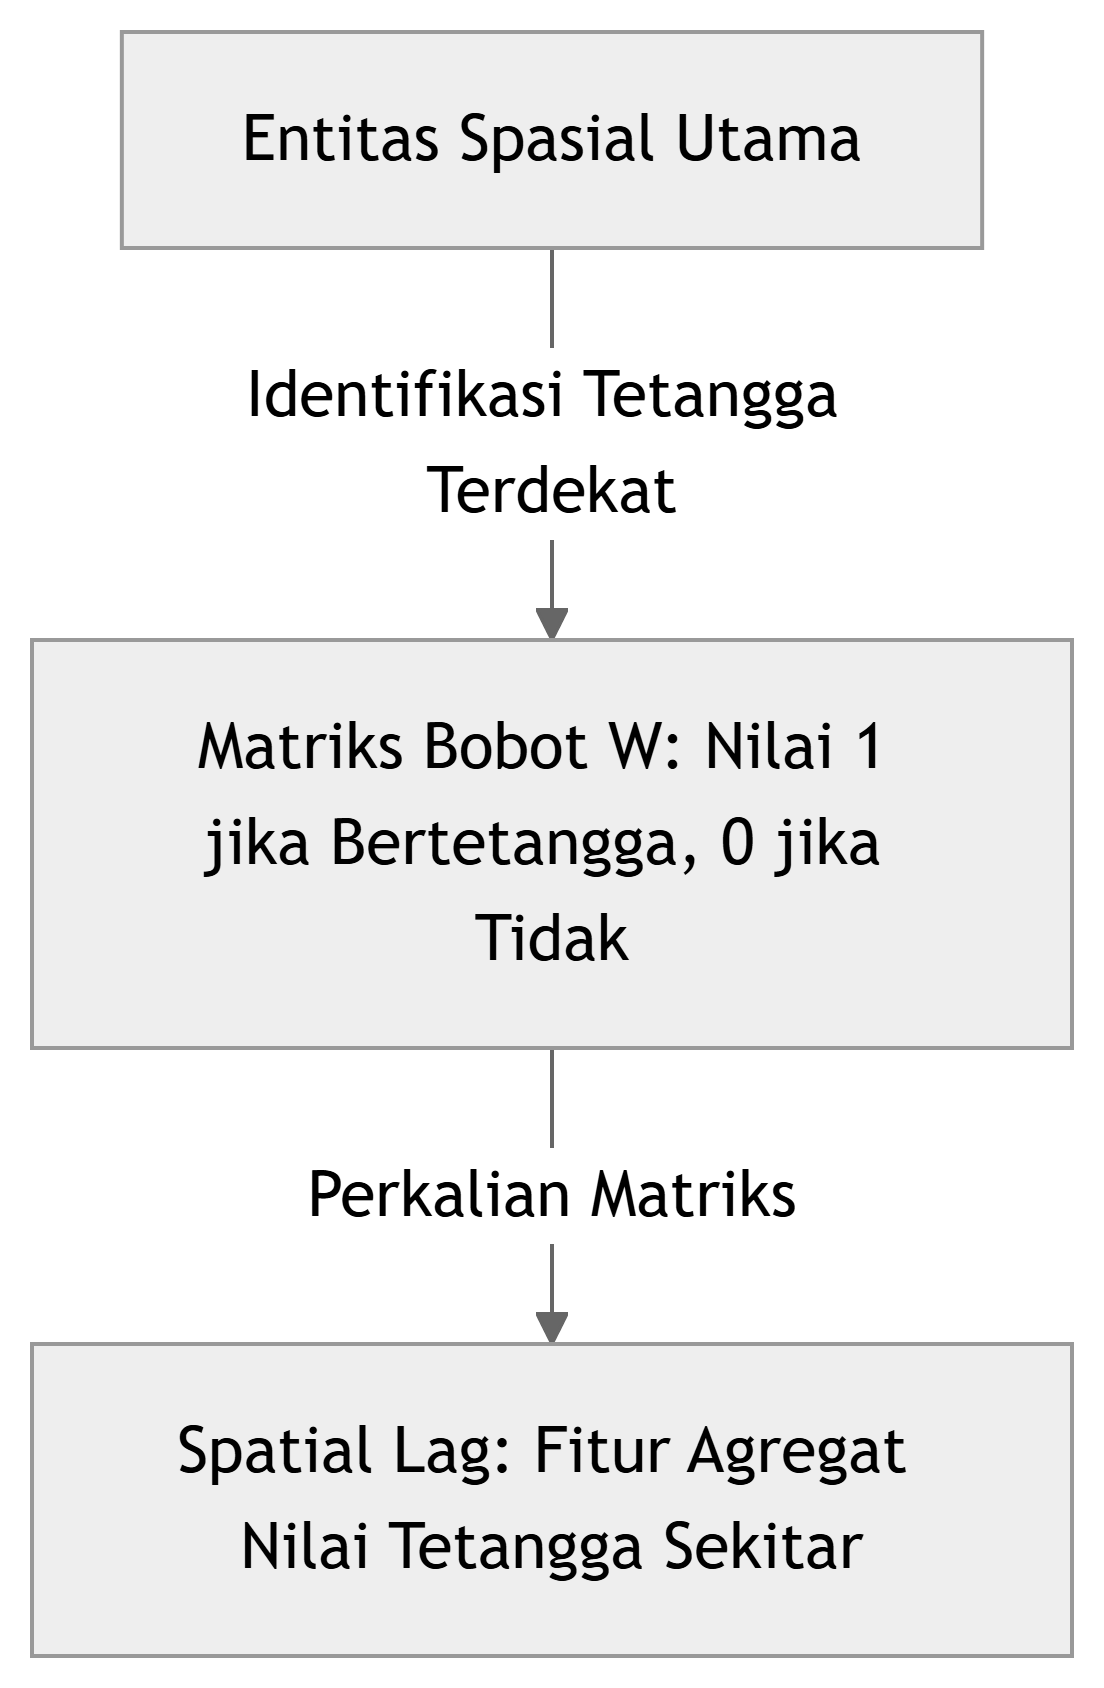
\includegraphics[width=\linewidth,height=0.72\textheight,keepaspectratio]{ch13-fig-8}
\caption{Subgraf Mencegah Kebocoran Set Pelatihan dan Set Uji}
\label{fig:ch13-fig-8}
\end{figure}

Desain pemisahan pada graf membedakan dua skenario evaluasi untuk mengelola masalah konektivitas ini:

\begin{enumerate}
\def\labelenumi{\arabic{enumi}.}
\tightlist
\item
  \textbf{Pembelajaran \emph{Transductive}:} Struktur graf secara keseluruhan dibiarkan terlihat selama fase pelatihan, namun label untuk simpul uji disembunyikan. Model membentuk representasi dengan melihat topologi jaringan secara utuh, yang rentan memicu kebocoran fitur tanpa pengawasan pembatasan yang ketat.
\item
  \textbf{Pembelajaran \emph{Inductive}:} Model dievaluasi pada subgraf yang terisolasi. Set uji dipisahkan secara fisik dari set pelatihan tanpa ada sisi penghubung, sehingga model dipaksa untuk mengenali pola hanya dari fitur dan topologi baru.
\end{enumerate}

Dampak buruk kebocoran ini sangat nyata pada kasus seperti deteksi penipuan keuangan. Jika pemisahan dilakukan secara acak, akun penipu di set pelatihan bisa memiliki riwayat transfer langsung ke akun di set uji. Sinyal penipuan tersebut akan ditarik melintasi sisi penghubung selama agregasi. Di lingkungan produksi, koneksi langsung seperti itu belum tentu tersedia, sehingga kinerja model akan anjlok.

Menerapkan \emph{praktik pipeline yang benar} menuntut perlindungan dan isolasi yang kaku. Strategi mitigasi standar yang lazim diadopsi meliputi:

\begin{itemize}
\tightlist
\item
  \textbf{Pemutusan Sisi Penghubung:} Menghapus seluruh sisi yang melintasi subgraf pelatihan dan pengujian sebelum proses pembentukan fitur dimulai, sehingga isolasi fisik pada evaluasi \emph{inductive} dapat dijamin keamanannya.
\item
  \textbf{Pemisahan Temporal:} Pada jejaring dinamis yang terus bertumbuh, model dilatih menggunakan struktur graf hingga batas waktu tertentu, kemudian dievaluasi murni pada simpul atau interaksi yang baru terbentuk setelah batas waktu tersebut.
\item
  \textbf{Isolasi \emph{Negative Sampling}:} Pada tugas prediksi tautan (\emph{link prediction}), pembangkitan pasangan simpul negatif harus dilakukan secara terpisah di masing-masing partisi agar model tidak menghafal ketidakhadiran sisi dari set pengujian.
\end{itemize}

\section{Studi Kasus: Prediksi Berbasis Lokasi dan Klasifikasi Simpul}\label{studi-kasus-prediksi-berbasis-lokasi-dan-klasifikasi-simpul}

Bagian ini membandingkan pendekatan pemodelan pada dua domain keruangan yang berbeda: dunia fisik dan struktur jaringan abstrak. Kedua studi kasus berikut mendemonstrasikan bahwa teknik ekstraksi representasi sangat menentukan batas kinerja dari sebuah model \emph{machine learning}.

\subsection{Kasus 1: Prediksi Harga Rumah (Domain Fisik)}\label{kasus-1-prediksi-harga-rumah-domain-fisik}

Pada kasus pertama, kita memprediksi harga rumah di suatu wilayah. Pendekatan ini dapat dikembangkan melalui beberapa tahapan representasi:

\begin{itemize}
\tightlist
\item
  \textbf{\emph{Baseline} Koordinat Mentah:} Titik awal pemodelan menggunakan algoritma berbasis pohon (\emph{random forest}) yang hanya menerima nilai absolut lintang dan bujur. Pendekatan ini umumnya hanya memberikan akurasi yang moderat. Oleh karena ruang fitur dibelah secara tegak lurus terhadap sumbu, algoritma terpaksa membuat banyak percabangan rumit hanya untuk memetakan efek jarak radial dari sebuah pusat tata kota.
\item
  \textbf{Injeksi Fitur Keruangan:} Kinerja model meningkat secara drastis setelah kita menyuntikkan fitur turunan yang mengkuantifikasi kedekatan lokasi. Alih-alih mengandalkan koordinat mentah, kita menambahkan metrik spasial seperti jarak fisik ke fasilitas umum (contohnya taman kota) serta nilai \emph{spatial lag} yang mengukur rata-rata pergerakan harga rumah di lingkungan terdekat. Pola ketetanggaan ini dikemas menjadi representasi yang \emph{dirancang manusia} agar siap diolah oleh model.
\item
  \textbf{Validasi \emph{Spatial Block}:} Eksperimen data spasial sangat rentan terhadap kebocoran informasi akibat autokorelasi geografis. Pengacakan data secara konvensional dapat menyebabkan model dilatih dengan data rumah di satu sisi jalan dan diuji dengan rumah di seberangnya. Oleh karena itu, kita perlu memisahkan area data latih dan uji secara geografis menggunakan metode \emph{spatial block cross-validation} beserta zona penyangga (\emph{buffer}).
\end{itemize}

\begin{lstlisting}[language=Python]
import numpy as np
import pandas as pd
from sklearn.cluster import KMeans
from sklearn.model_selection import GroupKFold
from sklearn.ensemble import RandomForestRegressor
from sklearn.metrics import mean_squared_error

# 1. Menyiapkan simulasi data geografis rumah (1000 titik koordinat)
np.random.seed(42)
lat = np.random.uniform(-6.3, -6.1, 1000)   # Koordinat Lintang
lon = np.random.uniform(106.7, 106.9, 1000) # Koordinat Bujur
# Simulasi harga yang dipengaruhi secara non-linier oleh posisi koordinat
harga = 500 + (lon - 106.7) * 2000 - (lat + 6.2) * 1500 + np.random.normal(0, 50, 1000)

df = pd.DataFrame({'Latitude': lat, 'Longitude': lon, 'Harga': harga})

# 2. Pembentukan "Spatial Blocks" via Clustering KMeans pada koordinat lokasi
# Membagi wilayah pengamatan secara geografis menjadi 10 blok regional terpisah
coords = df[['Latitude', 'Longitude']]
kmeans = KMeans(n_clusters=10, random_state=42, n_init=10)
df['Spatial_Block'] = kmeans.fit_predict(coords)

# 3. Menjalankan GroupKFold berdasarkan pembagian Spatial Block
# Teknik ini menjamin set latih dan uji terisolasi secara spasial (mencegah autokorelasi)
gkf = GroupKFold(n_splits=5)
mse_scores = []

print("--- Hasil Spatial Block Cross-Validation ---")
for fold, (train_idx, test_idx) in enumerate(gkf.split(df, groups=df['Spatial_Block']), 1):
    X_train, X_test = df.iloc[train_idx][['Latitude', 'Longitude']], df.iloc[test_idx][['Latitude', 'Longitude']]
    y_train, y_test = df.iloc[train_idx]['Harga'], df.iloc[test_idx]['Harga']
    
    # Model dilatih hanya pada blok regional pelatihan
    model = RandomForestRegressor(n_estimators=50, random_state=42)
    model.fit(X_train, y_train)
    
    # Pengujian murni dilakukan pada blok regional uji yang terpisah fisik
    y_pred = model.predict(X_test)
    mse = mean_squared_error(y_test, y_pred)
    mse_scores.append(mse)
    
    train_blocks = df.iloc[train_idx]['Spatial_Block'].unique()
    test_blocks = df.iloc[test_idx]['Spatial_Block'].unique()
    
    print(f"Fold {fold}:")
    print(f"   - Blok Latih: {train_blocks}")
    print(f"   - Blok Uji  : {test_blocks} (Isolasi Terpenuhi)")
    print(f"   - MSE       : {mse:.2f}")

print(f"\nRata-rata MSE Lintas Blok Spasial: {np.mean(mse_scores):.2f}")
\end{lstlisting}

\subsection{Kasus 2: Klasifikasi Topik Makalah (Domain Jaringan Abstrak)}\label{kasus-2-klasifikasi-topik-makalah-domain-jaringan-abstrak}

Studi kasus kedua beralih dari peta geografis ke graf sitasi makalah (seperti dataset Cora). Tujuannya adalah mengklasifikasikan topik subjek dari suatu makalah akademik (simpul) berdasarkan pola kutipannya (sisi).

Evolusi representasi pada graf ini terlihat dari perbandingan tiga tingkatan model:

\begin{itemize}
\tightlist
\item
  \textbf{\emph{Baseline} Fitur Struktural:} Pendekatan awal mengandalkan fitur struktural dasar, yaitu perhitungan \emph{in-degree} dan \emph{out-degree} pada setiap simpul. Pendekatan ini menghasilkan performa yang rendah karena tingginya frekuensi kutipan sebuah makalah tidak selalu mencerminkan rumpun keilmuannya secara akurat.
\item
  \textbf{\emph{Embedding} dengan \emph{Random Walk}:} Konteks relasi antar-topik mulai tertangkap ketika kita beralih ke representasi yang \emph{dipelajari mesin}. Algoritma seperti \emph{Node2Vec} menelusuri graf dan membangun vektor \emph{embedding}. Setelah kompleksitas topologi diringkas menjadi representasi padat berdimensi rendah, sebuah model klasifikasi linier biasa sudah mampu memetakan makalah ke dalam topik yang tepat.
\item
  \textbf{Pembaruan Representasi dengan GNN:} Akurasi tertinggi dicapai dengan menggunakan arsitektur \emph{Graph Neural Network} (GNN). GNN secara terintegrasi meleburkan fitur teks dari isi makalah dengan struktur jaringan sitasinya. Setiap simpul akan bertukar pesan dengan makalah tetangganya demi memperbarui nilai representasinya sendiri.
\end{itemize}

Mekanisme pertukaran pesan untuk pembaruan representasi pada GNN umumnya diformulasikan sebagai berikut:

\[ h_v^{(l)} = \sigma \left( W^{(l)} \cdot \text{AGGREGATE}\left(\{h_u^{(l-1)} : u \in \mathcal{N}(v) \} \right) \right) \]

Di mana:

\begin{itemize}
\tightlist
\item
  \(h_v^{(l)}\) merepresentasikan vektor fitur dari simpul \(v\) pada lapisan ke-\(l\).
\item
  \(\sigma\) merupakan fungsi aktivasi non-linier (seperti ReLU).
\item
  \(W^{(l)}\) adalah matriks bobot yang dipelajari selama proses pelatihan pada lapisan tersebut.
\item
  \(\mathcal{N}(v)\) menunjukkan himpunan simpul tetangga yang terhubung langsung dengan simpul \(v\).
\item
  \(\text{AGGREGATE}\) adalah fungsi matematika (misalnya rata-rata atau penjumlahan) yang meleburkan informasi dari simpul-simpul tetangga.
\end{itemize}

{[}GAMBAR 13.6: Skema - Subgraf representasi pada proses pertukaran pesan antar simpul dalam graf sitasi{]}

Persamaan di atas memperjelas bahwa representasi sebuah makalah pada arsitektur GNN tidak berdiri sendiri, melainkan secara aktif dibentuk oleh agregasi informasi dari subgraf tetangganya. Kedua studi kasus ini memberikan benang merah yang sejalan: cara pengekstraksian dan penyajian struktur ketetanggaan ke dalam model memiliki dampak yang sama besarnya dengan pilihan arsitektur algoritmanya.

% ==========================================================================
% ch14.tex — dihasilkan dari v2/drafts oleh tools/md2tex.py
% Sumber: v2\drafts\ch14\ch14_draft_v2.md
% Boleh disunting manual; menjalankan md2tex.py lagi akan menimpa.
% ==========================================================================
\chapter{Data Multimodal}\label{data-multimodal}

Data multimodal menggabungkan dua atau lebih modalitas, seperti tabular, teks, citra, audio, atau lokasi, yang semuanya menggambarkan entitas yang sama. Tantangannya bukan menumpuk fitur sebanyak mungkin. Setiap modalitas memiliki kelengkapan, \emph{noise}, dan representasi yang berbeda. Jika potongan-potongan itu disatukan pada entitas atau skala yang salah, model menerima contoh belajar yang rusak. Karena itu, langkah pertama adalah memastikan semua potongan data merujuk ke unit yang sama. Setelah itu, representasi digabung, diseimbangkan, dan dibuat tahan terhadap modalitas yang hilang.

Bab ini membahas strategi penggabungan (fusion) pada tingkat fitur awal, tingkat menengah, dan tingkat keputusan (Baltrušaitis et al. 2019). Konkatenasi fitur dibahas bersama masalah ketimpangan dimensi antar modalitas. Strategi penanganan modalitas yang hilang saat produksi, ruang embedding bersama (joint embedding) untuk perbandingan lintas modalitas, dan model multimodal pratelatih dibahas sebagai pilihan yang tersedia. Bab ini menguraikan bahwa keberhasilan multimodal berangkat dari mempertemukan modalitas pada unit yang benar.

\section{\texorpdfstring{Apa Itu Data Multimodal? \emph{Alignment} dan Sinkronisasi Waktu}{Apa Itu Data Multimodal? Alignment dan Sinkronisasi Waktu}}\label{apa-itu-data-multimodal-alignment-dan-sinkronisasi-waktu}

Pada tabel biasa, struktur baris membuat kolom otomatis sejajar. Contoh kerja pada bab ini memakai Open Food Facts, kumpulan catatan produk makanan yang menggabungkan nama produk, daftar bahan, kategori, nutrisi, dan thumbnail. Setiap baris mewakili satu produk makanan, sedangkan Nutri-Score dapat dipakai untuk membangun target ringkas. Pada data multimodal, ``baris'' seperti itu harus dibangun dan diaudit. Foto produk harus dipasangkan dengan produk yang benar, bukan produk lain; teks bahan harus berasal dari kemasan yang sama, bukan hasil gabungan dari item serupa.

\emph{Alignment} menjawab pertanyaan: potongan dari modalitas berbeda mana yang merujuk pada entitas, peristiwa, atau interval waktu yang sama? Jika teks bahan atau kategori dipasangkan dengan foto produk yang salah, sampel belajar menjadi bising. Jika sinyal masa depan dipasangkan dengan prediksi masa lalu, masalahnya lebih parah: \emph{leakage}.

Untuk \emph{stream}, sinkronisasi waktu menjadi pusat. Video dapat memiliki 30 \emph{frame} per detik, sedangkan audio memiliki 44.100 \emph{sample} per detik. Jika unit observasi adalah satu detik, satu contoh belajar dapat memuat 30 \emph{frame} video, 44.100 \emph{sample} audio, dan beberapa pembacaan sensor. Gagasan \emph{window} dari Bab 10 dapat diperluas lintas modalitas.

\[
W_{\tau} = \{ (x_k^{(m)}, t_k) \mid \tau \le t_k < \tau + \Delta t \}
\]

Dalam rumus tersebut, \(W_{\tau}\) adalah \emph{window} yang dimulai pada waktu \(\tau\), \(\Delta t\) adalah lebarnya, \(x_k^{(m)}\) adalah titik data ke-\(k\) dari modalitas \(m\), dan \(t_k\) adalah \emph{timestamp}-nya. Satu unit observasi mengumpulkan semua titik dari berbagai modalitas yang jatuh di dalam \emph{window} tersebut.

Gambar 14.1 memperlihatkan tiga timeline dengan kepadatan berbeda. Window satu detik memotong video, audio, dan sensor menjadi satu blok observasi yang sejajar.

\begin{figure}[tbp]\centering
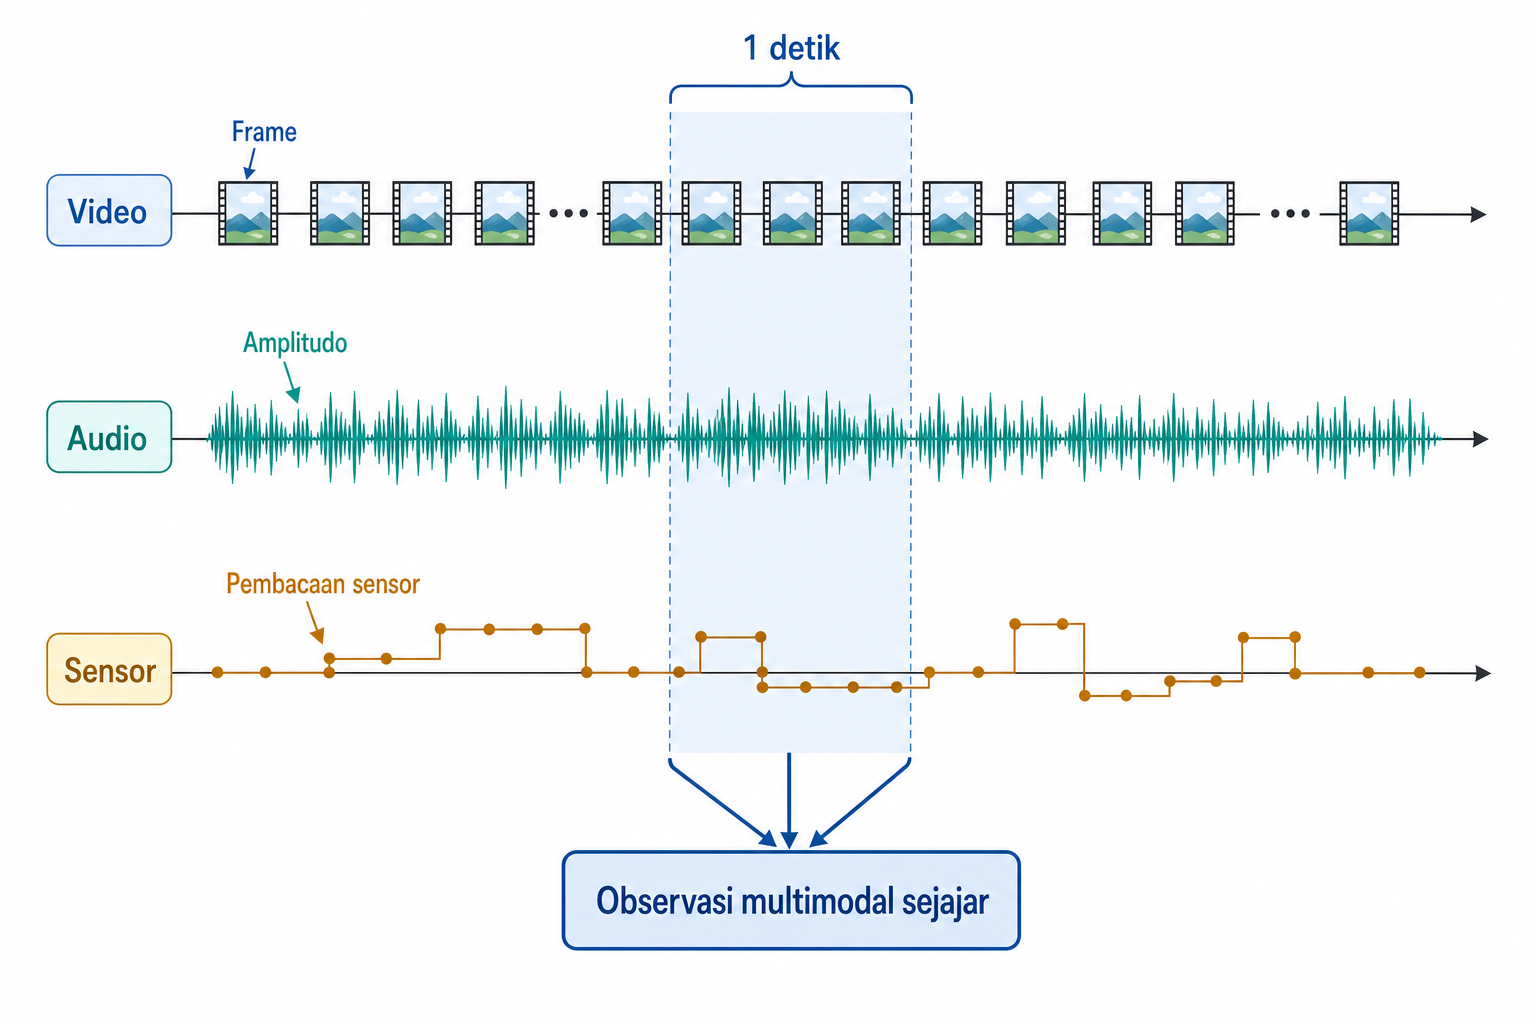
\includegraphics[width=111.6mm]{ch14-fig-1}
\caption{Alignment window untuk video, audio, dan sensor}
\label{fig:ch14-fig-1}
\end{figure}

Sample unit dari Bab 1 tetap menjadi keputusan awal. Pada contoh Open Food Facts di bab ini, unitnya adalah produk makanan; target ringkasnya dibangun dari Nutri-Score, dan modalitas yang digabung adalah nutrisi tabular, teks, dan thumbnail. Split juga harus menjaga integritas entitas: semua modalitas dari satu produk berada di sisi split yang sama. Jika teks produk berada di training tetapi gambarnya berada di test, model dapat mengenali entitas melintasi batas split.

Contoh Open Food Facts ini sengaja memakai label turunan: \passthrough{\lstinline!nutri_good!} dibentuk dari Nutri-Score, sedangkan cabang nutrisi tabular memuat bidang-bidang yang secara substansial menentukan Nutri-Score. Karena itu, nutrisi tabular merupakan \emph{near-label signal}, yaitu sinyal yang sangat dekat dengan definisi label, sehingga performanya yang kuat memang diharapkan. Contoh ini dipakai untuk mengajarkan label turunan; hasilnya bukan bukti bahwa fitur nutrisi atau \emph{fusion} selalu dominan pada tugas lain, dan \emph{fusion} sendiri tidak otomatis lebih baik.

Sebagian model \emph{vision-language} modern mulai menyerap sebagian \emph{alignment} temporal ke dalam arsitektur, misalnya dengan menangani \emph{frame rate} yang bervariasi. Itu adalah tren penting, tetapi tidak menghapus pertanyaan dasar bab ini. Kita tetap harus mendefinisikan unit observasi, batas waktu, dan integritas entitas sebelum fitur multimodal dapat dipercaya. Setelah potongan data sudah sejajar, keputusan berikutnya adalah titik pertemuan antar modalitas: apakah digabung sebelum model, di dalam model, atau setelah model membuat prediksi.

\section{\texorpdfstring{Strategi \emph{Fusion}: Early, Intermediate, Late, serta Tingkat Fitur vs.~Keputusan}{Strategi Fusion: Early, Intermediate, Late, serta Tingkat Fitur vs.~Keputusan}}\label{strategi-fusion-early-intermediate-late-serta-tingkat-fitur-vs.-keputusan}

Setelah modalitas disejajarkan, titik penggabungannya perlu ditentukan. \emph{Fusion} bukan satu teknik tunggal, melainkan keputusan tentang pertemuan antarrepresentasi sebelum model, di dalam model, atau setelah model menghasilkan prediksi.

\emph{Early fusion} menggabungkan fitur mentah atau fitur rendah sebelum masuk ke model utama. Pada Open Food Facts, fitur nutrisi dapat digabung dengan fitur teks bahan atau embedding thumbnail, lalu satu model membaca semuanya. Pendekatan ini sederhana dan memungkinkan model mempelajari interaksi langsung antarfitur. Namun, ia sensitif terhadap skala, \emph{missing modality}, dan ketimpangan dimensi. Masalah itu menjadi fokus Bagian 14.3.

\emph{Intermediate fusion} menggabungkan representasi laten di dalam arsitektur. Setiap modalitas dapat memiliki \emph{encoder} sendiri: teks masuk ke \emph{text encoder}, citra masuk ke \emph{image encoder}, audio masuk ke \emph{audio encoder}. \emph{Embedding} yang dihasilkan bertemu di \emph{hidden layer}. Ini memungkinkan interaksi lebih kaya, tetapi membutuhkan lebih banyak data, komputasi, dan desain model.

\emph{Late fusion} menggabungkan prediksi atau keputusan dari model yang berbeda. Misalnya, model nutrisi memberi probabilitas tinggi untuk produk bernutrisi baik, sedangkan model gambar memberi sinyal lemah dari thumbnail; \emph{ensemble} merata-ratakan atau menimbang dua probabilitas itu. Representasinya tidak dicampur. Yang digabung adalah output. \emph{Late fusion} modular dan lebih tahan ketika satu modalitas hilang, tetapi dapat kehilangan interaksi lintas modalitas yang hanya terlihat jika fitur bertemu lebih awal. Secara konseptual, \emph{early fusion} dan \emph{intermediate fusion} bekerja pada tingkat representasi (\emph{feature-level fusion}), sedangkan \emph{late fusion} bekerja pada tingkat keputusan (\emph{decision-level fusion}).

Gambar 14.2 menunjukkan tiga titik gabung itu pada dua modalitas yang sama. Perhatikan bahwa yang berubah bukan hanya diagramnya, tetapi juga jenis interaksi yang mungkin dipelajari.

\begin{figure}[tbp]\centering
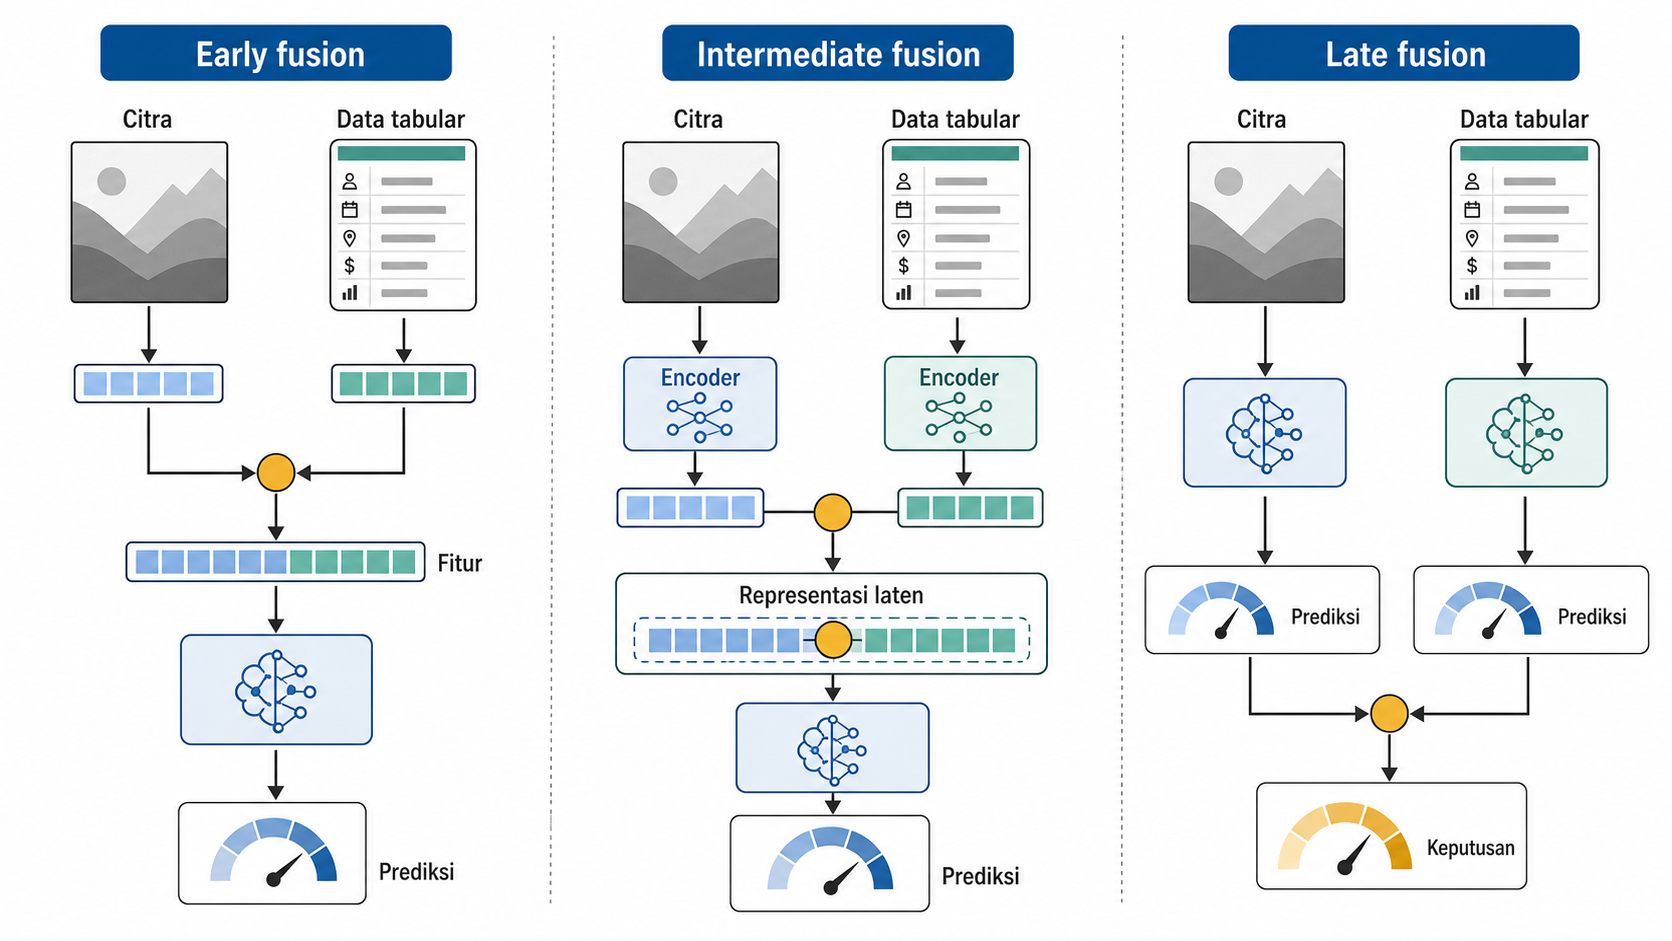
\includegraphics[width=111.6mm]{ch14-fig-2}
\caption{Tiga titik \emph{fusion} multimodal}
\label{fig:ch14-fig-2}
\end{figure}

Tabel 14.1 merangkum pilihan \emph{fusion}. Barisnya bergerak dari pendekatan paling sederhana sampai paling fleksibel, bukan membentuk \emph{ranking}. Kolom risiko menunjukkan pengujian yang perlu didahulukan. \emph{Early fusion} menuntut kontrol skala dan dimensi, \emph{intermediate fusion} menuntut data dan desain, sedangkan \emph{late fusion} menuntut aturan penggabungan prediksi. Pilihan yang tepat bergantung pada ukuran data, biaya, \emph{missingness}, dan kebutuhan interaksi.

\tabeljudul{Tabel 14.1 — Strategi fusi multimodal}

{\def\LTcaptype{none} % do not increment counter
\par\vspace{3pt}\noindent
\begingroup\renewcommand{\arraystretch}{1.0}%
\scriptsize\linespread{1}\selectfont
\renewcommand{\_}{\textunderscore\hspace{0pt}}%
\begin{xltabular}{\linewidth}{@{}>{\raggedright\arraybackslash}p{(\linewidth-8\tabcolsep)*\real{0.160}} >{\raggedright\arraybackslash}p{(\linewidth-8\tabcolsep)*\real{0.160}} >{\raggedright\arraybackslash}p{(\linewidth-8\tabcolsep)*\real{0.217}} >{\raggedright\arraybackslash}p{(\linewidth-8\tabcolsep)*\real{0.281}} >{\raggedright\arraybackslash}p{(\linewidth-8\tabcolsep)*\real{0.182}}@{}}
\toprule

Strategi
 & 
Apa yang digabung
 & 
Kekuatan
 & 
Risiko
 & 
Penggunaan khas
 \\
\midrule
\endhead




\emph{Early fusion} & Vektor fitur & Interaksi lintas modalitas dipelajari langsung & Ketimpangan dimensi\slash{}skala, rapuh pada modalitas hilang & Tabular + \emph{embedding} sederhana \\
\emph{Intermediate fusion} & Representasi laten & Interaksi kaya di dalam model & Butuh data\slash{}komputasi dan desain arsitektur & \emph{Deep learning} multimodal \\
\emph{Late fusion} & Prediksi atau keputusan & Modular, tahan modalitas hilang & Kehilangan sebagian interaksi lintas modalitas & \emph{Ensemble} model per modalitas \\
\bottomrule
\end{xltabular}\endgroup\par\vspace{5pt}

}

Ada juga arsitektur \emph{frontier} seperti \emph{latent bottleneck} ala Perceiver, yang melewatkan berbagai \emph{input} melalui sekumpulan \emph{latent vectors} tetap. Gagasan itu memisahkan kedalaman model dari panjang \emph{input}. Dalam rekayasa fitur praktis, keputusan dasarnya tetap menyangkut titik pertemuan modalitas, bentuk representasinya, dan konsekuensi bagi validasi.

\section{Konkatenasi Fitur dan Keseimbangan Dimensi}\label{konkatenasi-fitur-dan-keseimbangan-dimensi}

Bentuk \emph{early fusion} yang paling mudah adalah konkatenasi: letakkan vektor fitur dari beberapa modalitas berdampingan (Ngiam et al. 2011). Secara notasi:

\[
\mathbf{x}_{\text{gabungan}} = [\, \mathbf{x}_{\text{tab}} \oplus \mathbf{x}_{\text{teks}} \oplus \mathbf{x}_{\text{citra}} \,] \in \mathbb{R}^{d_{\text{tab}} + d_{\text{teks}} + d_{\text{citra}}}
\]

Dalam rumus tersebut, \(\oplus\) berarti konkatenasi. Masalahnya terlihat langsung dari dimensi \(d_{\text{tab}}\), \(d_{\text{teks}}\), dan \(d_{\text{citra}}\). Jika \emph{image embedding} berdimensi 2048 digabung dengan 10 fitur tabular, lebih dari 99\% dimensi berasal dari citra. Jika \emph{text embedding} berdimensi 768 digabung dengan 20 fitur transaksi, cabang teks mendominasi jumlah koordinat.

Jumlah dimensi dapat berkontribusi pada dominasi modalitas, tetapi tidak menjaminnya. Pada model berbasis jarak, banyak koordinat dari satu cabang dapat mengendalikan \emph{proximity} jika skala dan normalisasinya tidak ditata. Pada model \emph{gradient-based}, pengaruh tiap cabang juga bergantung pada arsitektur, normalisasi, regularisasi, penskalaan, dan kekuatan sinyal tugas. Cabang berdimensi kecil tetap dapat dominan bila sinyalnya jauh lebih kuat. Ini adalah pelajaran Bab 3 pada skala \emph{fusion}.

Penskalaan fitur perlu dilakukan dengan hati-hati dan tetap di dalam \emph{pipeline} validasi. Setiap transformasi per modalitas, seperti standardisasi, PCA, atau proyeksi, harus di-\emph{fit} pada data latih saja, lalu di-\emph{transform} ke kedua split, persis seperti prinsip Bab 2. Namun, penskalaan saja tidak selalu cukup. Dua strategi umum adalah mengecilkan mayoritas atau mengangkat minoritas. Mengecilkan mayoritas dapat dilakukan dengan \emph{dimensionality reduction}, \emph{pooling}, atau \emph{feature selection}. TruncatedSVD cocok untuk representasi berdimensi tinggi yang jarang, misalnya \emph{TF-IDF} dari Bab 11. Untuk \emph{embedding} padat seperti keluaran BERT atau ResNet, PCA/SVD, proyeksi yang dipelajari (\emph{learned projection}), dan \emph{feature selection} adalah pilihan yang perlu dibandingkan dalam validasi; proyeksi yang dipelajari tidak otomatis lebih aman. Mengangkat minoritas dapat dilakukan dengan \emph{learned embedding layer} kecil yang memetakan fitur tabular ke lebar yang lebih sebanding.

Gambar 14.3 menggambarkan ketimpangan itu secara visual. \emph{Sliver} fitur tabular dapat tenggelam di samping blok \emph{embedding} yang sangat panjang; dua solusi dasarnya adalah memampatkan blok besar atau memperlebar cabang kecil.

\begin{figure}[tbp]\centering
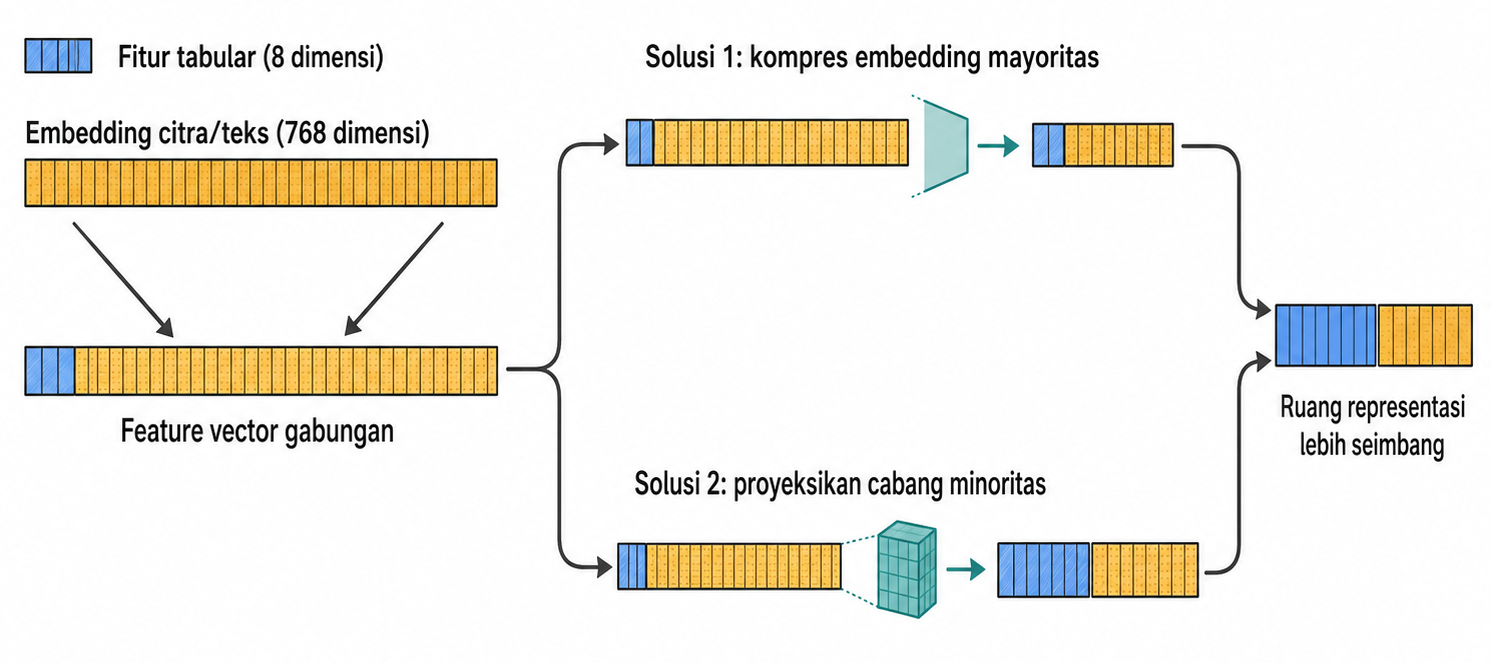
\includegraphics[width=111.6mm]{ch14-fig-3}
\caption{Menyeimbangkan dimensi representasi pada fusi multimodal}
\label{fig:ch14-fig-3}
\end{figure}

Pertanyaan evaluasinya sederhana: apakah setiap modalitas menambah nilai? Bab 9 memberi alatnya, yaitu \emph{ablation} per kelompok fitur. Pada Open Food Facts, latih model dengan nutrisi saja, teks saja, gambar saja, dan gabungan. Jika gabungan tidak mengalahkan cabang terbaik secara stabil, \emph{fusion} mungkin hanya menambah kompleksitas. Setelah dimensi dibuat seimbang, asumsi berikutnya adalah semua cabang tersedia. Pada sistem nyata, asumsi itu sering patah.

\begin{pendalaman}{Jembatan yang dipelajari: \emph{cross-attention} menggantikan konkatenasi}
Sistem multimodal modern makin sering mengganti konkatenasi buta dengan jembatan yang dipelajari. \emph{Cross-attention} \(\text{Attention}(Q, K, V) = \operatorname{softmax}\!\big(QK^{\top}/\sqrt{d_k}\big)V\) membuat satu modalitas, misalnya instruksi teks sebagai \emph{query} \(Q\), menarik fitur relevan dari modalitas lain, misalnya region citra sebagai \emph{keys} \(K\) dan \emph{values} \(V\). BLIP-2 memakai Q-Former sebagai jembatan kecil antara \emph{image encoder} beku dan LLM beku. Untuk proyek tabular berskala biasa, konkatenasi yang diseimbangkan tetap \emph{baseline} jujur yang perlu dikalahkan.
\end{pendalaman}

\section{Menangani Modalitas yang Hilang}\label{menangani-modalitas-yang-hilang}

Keseimbangan dimensi mengandaikan setiap cabang representasi hadir. Pada produksi, tidak semua sampel memiliki semua modalitas. Product listing dapat tidak memiliki gambar, teks bahan dapat kosong, atau nutrisi tabular dapat tidak lengkap. Pada domain lain, sensor bisa offline selama beberapa menit, audio dapat rusak, video gelap, atau teks kosong.

\emph{Missing modality} berbeda dari \emph{missing value} dalam satu tabel. Jika satu angka hilang, kita dapat memakai strategi seperti indikator dan imputasi sebagaimana Bab 5. Jika seluruh \emph{image embedding} atau \emph{audio branch} hilang, kita kehilangan satu representasi lengkap. Mengisi seluruh \emph{embedding} dengan rata-rata dataset sering hanya menciptakan titik buatan yang dapat dimanfaatkan model sebagai jalan pintas, bukan informasi asli tentang sampel tersebut.

Strategi bergantung pada desain \emph{fusion}. Pada \emph{early fusion}, salah satu opsi adalah vektor nol ditambah indikator \emph{missing}. Mask eksplisit atau \emph{learned missing token} merupakan alternatif ketika arsitektur mendukungnya. Vektor nol hanyalah placeholder numerik, bukan padanan literal ``citra hitam'' atau ``audio diam''; model perlu memperoleh penanda yang membedakannya dari nilai nol yang sah. Pada \emph{late fusion}, cabang yang hilang dapat dilewati, lalu prediksi dari cabang lain tetap dipakai. Pada pelatihan, \emph{modality dropout} dapat menyembunyikan modalitas secara acak agar model belajar bertahan dengan input parsial. Jika \emph{encoder} sudah diselaraskan dalam \emph{shared space}, modalitas yang tersisa kadang dapat menjadi substitusi kasar bagi modalitas yang hilang, tetapi kecukupannya harus divalidasi untuk tugas tersebut.

Tabel 14.2 merangkum strategi ini. Kolom ``cocok dengan fusi'' penting karena solusi untuk \emph{early fusion} tidak selalu cocok untuk \emph{late fusion}.

\tabeljudul{Tabel 14.2 — Strategi modalitas hilang}

{\def\LTcaptype{none} % do not increment counter
\par\vspace{3pt}\noindent
\begingroup\renewcommand{\arraystretch}{1.0}%
\scriptsize\linespread{1}\selectfont
\renewcommand{\_}{\textunderscore\hspace{0pt}}%
\begin{xltabular}{\linewidth}{@{}>{\raggedright\arraybackslash}p{(\linewidth-6\tabcolsep)*\real{0.186}} >{\raggedright\arraybackslash}p{(\linewidth-6\tabcolsep)*\real{0.338}} >{\raggedright\arraybackslash}p{(\linewidth-6\tabcolsep)*\real{0.160}} >{\raggedright\arraybackslash}p{(\linewidth-6\tabcolsep)*\real{0.316}}@{}}
\toprule

Strategi
 & 
Mekanisme
 & 
Cocok dengan fusi
 & 
Perhatian
 \\
\midrule
\endhead




Vektor nol + indikator & Isi cabang kosong dengan nol dan tandai absennya modalitas & \emph{Early fusion} & Salah satu opsi; nol bukan citra hitam atau audio hening \\
Mask atau \emph{learned missing token} & Tandai cabang hilang melalui mekanisme arsitektur & \emph{Early\slash{}intermediate fusion} & Perlu dilatih pada pola \emph{missingness} yang relevan \\
Lewati cabang & Pakai prediksi dari cabang yang tersedia & \emph{Late fusion} & Perlu aturan agregasi untuk input parsial \\
\emph{Modality dropout} saat pelatihan & Sembunyikan modalitas acak selama pelatihan & \emph{Intermediate\slash{}early fusion} & \emph{Dropout} harus menyerupai \emph{missingness} nyata \\
Substitusi ruang bersama & Pakai \emph{embedding} modalitas tersisa dalam \emph{shared space} & \emph{Joint embedding} & Hanya masuk akal bila ruang benar-benar selaras \\
Model terpisah per subset modalitas & Latih model untuk kombinasi modalitas tertentu & Semua & Kompleksitas pemeliharaan meningkat \\
\bottomrule
\end{xltabular}\endgroup\par\vspace{5pt}

}

Pola missingness sendiri dapat informatif atau bias. Produk tanpa gambar bisa berasal dari sumber data tertentu, kategori tertentu, atau item yang belum lengkap proses unggahnya. Teks bahan yang kosong tidak sama dengan bahan yang memang sederhana. Karena itu, dropping semua sampel tidak lengkap jarang menjadi default yang baik. Sistem harus mendefinisikan perilaku untuk input parsial sebelum deployment.

Aturan split dari Bagian 14.1 juga berlaku di sini. Semua modalitas milik satu entitas harus berada di sisi split yang sama, termasuk modalitas yang hilang. Jika tidak, model dapat belajar mengenali entitas melalui cabang lain dan membuat evaluasi tampak lebih kuat daripada kenyataannya. Salah satu cara menangani modalitas hilang adalah shared space substitution; untuk memahami kapan itu masuk akal, kita perlu melihat bagaimana ruang bersama lintas modalitas dipelajari.

\section{\texorpdfstring{\emph{Cross-Modal} dan \emph{Joint Embedding}}{Cross-Modal dan Joint Embedding}}\label{cross-modal-dan-joint-embedding}

Concatenation menggabungkan fitur dari beberapa modalitas, tetapi tidak membuat piksel dan kata menjadi sebanding secara langsung. Nilai piksel, word frequency, dan audio frame tidak memiliki korespondensi matematis alami. Agar teks ``sepatu merah'' dekat dengan gambar sepatu merah, ruang bersama itu harus dipelajari dari pasangan data.

\emph{Cross-modal} atau \emph{joint embedding} memetakan modalitas berbeda ke ruang vektor yang sama. Pada pelatihan bergaya CLIP (Radford et al. 2021), \emph{image encoder} dan \emph{text encoder} dilatih memakai pasangan \emph{image-text}. Pasangan yang cocok ditarik mendekat, sedangkan pasangan acak didorong menjauh. Dengan demikian, citra dan teks yang merujuk pada objek atau konsep serupa berada dekat dalam \emph{embedding space}.

Secara notasi, dua encoder dapat ditulis:

\[
\mathbf{z}_{\text{img}} = f_{\theta}(\mathbf{x}_{\text{img}})
\]

\[
\mathbf{z}_{\text{teks}} = g_{\phi}(\mathbf{x}_{\text{teks}})
\]

Encoder citra \(f_{\theta}\) dan encoder teks \(g_{\phi}\) memproyeksikan input ke ruang \(\mathbb{R}^d\) yang sama. Kedekatan dapat dibandingkan dengan cosine similarity, seperti formula yang sudah dipakai pada Bab 11.

Pada model bergaya CLIP, \emph{embedding} dinormalisasi L2 ketika \emph{dot product} dipakai untuk merepresentasikan cosine similarity. Tanpa normalisasi itu, \emph{dot product} juga dipengaruhi magnitudo vektor.

Gambar 14.4 memperlihatkan arsitektur dual encoder. Image encoder dan text encoder terpisah, tetapi keluarannya hidup di satu ruang. Query teks dapat menarik gambar yang paling dekat.

\begin{figure}[tbp]\centering
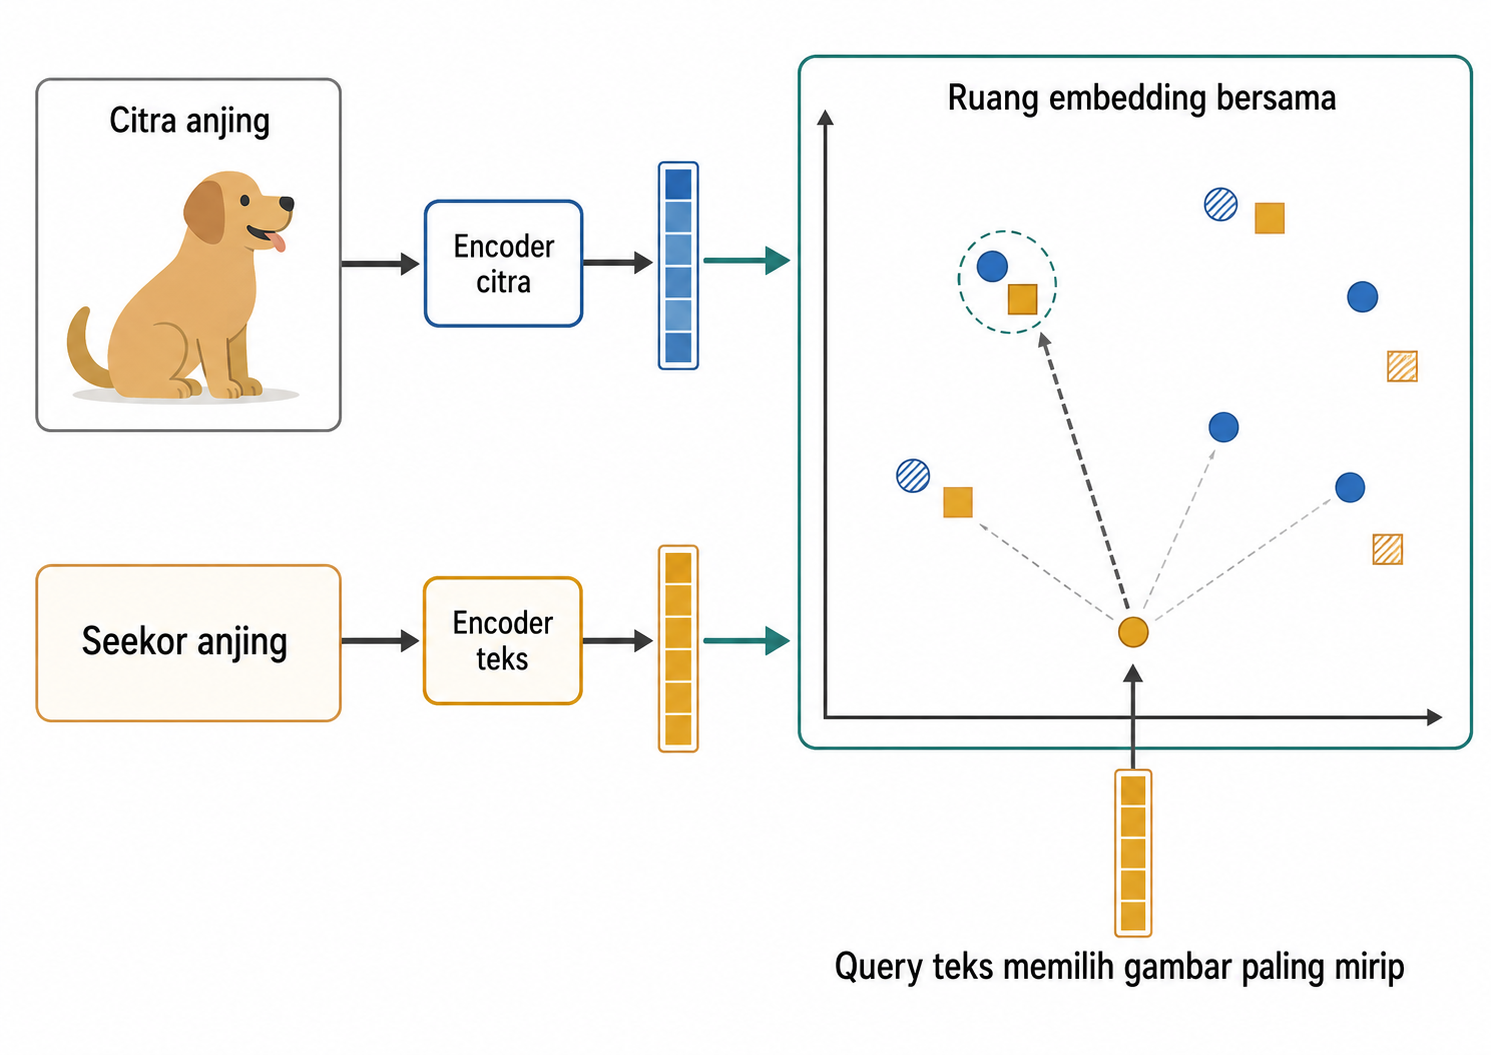
\includegraphics[width=111.6mm]{ch14-fig-4}
\caption{\emph{Dual encoder} dalam ruang \emph{embedding} bersama}
\label{fig:ch14-fig-4}
\end{figure}

\emph{Joint embedding} mendukung \emph{retrieval}, \emph{zero-shot classification}, \emph{matching}, \emph{clustering}, dan \emph{multimodal search}. Dalam e-commerce, pengguna dapat mencari gambar produk dengan \emph{query} teks. Dalam arsip bukti, deskripsi tekstual dapat dipakai untuk menemukan citra atau audio yang relevan. \emph{Retrieval} teks-ke-audio memerlukan model yang memang diselaraskan pada pasangan audio-teks; encoder citra-teks tidak otomatis menyediakan keselarasan itu. Evaluasinya pun \emph{retrieval-shaped}: \emph{recall@k} menanyakan apakah pasangan benar muncul dalam k kandidat teratas, sedangkan \emph{nDCG} menilai kualitas \emph{ranking}. Metrik ini menggantikan akurasi klasifikasi biasa karena tugasnya adalah \emph{retrieval}, bukan klasifikasi label tunggal.

Namun, kedekatan \emph{embedding} bukan kebenaran mutlak. Ruang itu mencerminkan data pelatihan, kualitas \emph{pairing}, \emph{objective}, dan bias dataset. Jika pasangan data buruk, model belajar asosiasi buruk. Jika dataset kurang mewakili bahasa, budaya, atau domain tertentu, \emph{similarity} dapat menjadi tidak adil atau tidak relevan. Setelah ruang bersama terbukti berguna, langkah praktis berikutnya adalah memakai model \emph{pretrained} yang sudah membawa ruang semacam itu sebagai fitur siap pakai.

\begin{pendalaman}{\emph{Contrastive loss}, mesin yang menyejajarkan ruang}
Untuk \emph{batch} berisi \(N\) pasangan, salah satu arah \emph{objective} dapat ditulis \(\mathcal{L} = -\frac{1}{N} \sum_{i} \log \dfrac{\exp(\mathbf{v}_i \cdot \mathbf{t}_i / \tau)}{\sum_{j} \exp(\mathbf{v}_i \cdot \mathbf{t}_j / \tau)}\). Dalam rumus tersebut, \(\mathbf{v}_i\) adalah \emph{image embedding}, \(\mathbf{t}_i\) adalah \emph{caption embedding} pasangannya, dan \(\tau\) adalah \emph{temperature} yang mengatur ketajaman pemisahan. Setiap citra dilatih agar paling dekat dengan \emph{caption} miliknya sendiri di antara \emph{caption} lain dalam \emph{batch}. Dalam praktik CLIP, \emph{loss} ini simetris dan dihitung juga dari arah teks ke citra, sehingga kedua arah \emph{retrieval} terlatih. Keselarasan kontrasif mendukung \emph{retrieval}, tetapi tidak menjamin satu modalitas dapat menggantikan informasi khusus yang hilang dari modalitas lain; substitusi harus diuji pada tugas dan pola \emph{missingness} yang nyata.
\end{pendalaman}

\section{\texorpdfstring{Multimodal \emph{Pretrained} Model}{Multimodal Pretrained Model}}\label{multimodal-pretrained-model}

Jika ruang bersama sudah menjadi alat praktis, model multimodal \emph{pretrained} menawarkan encoder yang dapat dipakai ulang lintas modalitas. CLIP adalah contoh inti untuk \emph{image-text}. ImageBind memperluas ide \emph{shared embedding} ke lebih banyak modalitas. Model seperti ini dapat dipakai sebagai \emph{frozen feature extractor}, \emph{retrieval model}, atau komponen dalam sistem yang lebih besar.

Salah satu kemampuan yang membuatnya terkenal adalah \emph{zero-shot classification}. Untuk mengklasifikasikan citra tanpa pelatihan khusus pada tugas itu, kita dapat membuat beberapa \emph{prompt} teks kandidat, misalnya ``foto sepatu'', ``foto tas'', atau ``foto jam tangan''. Citra dan semua \emph{prompt} di-\emph{embed} ke ruang bersama, lalu label dipilih dari \emph{prompt} yang paling dekat. Dengan cara ini, klasifikasi berubah menjadi \emph{retrieval} dalam \emph{joint space}.

Kekuatan \emph{pretrained representation} tidak menghapus pekerjaan rekayasa fitur. \emph{Alignment} masih perlu jelas: citra mana dengan teks mana, frame mana dengan audio mana, entitas mana dengan metadata mana. \emph{Domain shift} tetap perlu diuji. Jika model dilatih pada data web umum, ia belum tentu adil atau akurat untuk citra medis, bahasa lokal, produk niche, atau data internal lembaga. \emph{Privacy} dan \emph{fairness} juga semakin penting karena model besar dapat membawa asosiasi dari data \emph{pretraining} yang tidak kita lihat langsung.

Reproducibility membutuhkan pencatatan yang lebih rinci. Nama model, versi, lisensi, \emph{preprocessing}, \emph{prompt text}, cara \emph{pooling}, penskalaan \emph{embedding}, dan \emph{metric similarity} semuanya bagian dari definisi fitur. Untuk \emph{zero-shot}, \emph{prompt wording} sendiri adalah keputusan rekayasa fitur. ``foto sepatu'' dan ``gambar produk sepatu'' dapat memberi \emph{ranking} berbeda, sehingga \emph{prompt} harus dicatat dan dievaluasi seperti fitur lain.

\begin{pendalaman}{Dari ekstraktor beku ke \emph{vision-language model}}
\emph{Frontier model} tidak selalu melatih ulang \emph{encoder} besar. BLIP-2, misalnya, memakai Q-Former sebagai jembatan yang belajar mengambil fitur visual relevan di antara \emph{image encoder} beku dan LLM beku. Model \emph{vision-language} yang lebih baru dapat mengonsumsi citra dan teks bersama, lalu menghasilkan representasi yang lebih mengikuti tugas daripada satu vektor tetap. Dalam lensa rekayasa fitur buku ini, sistem seperti itu tetap dapat dibaca sebagai \emph{extractor} dengan \emph{query} yang bisa diarahkan. Tugas \emph{reproducibility} justru bertambah: versi model, \emph{prompt}, \emph{preprocessing}, dan penskalaan harus dicatat lebih ketat. Bab 15 melanjutkan cerita umum tentang \emph{pretrained representation}, sedangkan Bab 16 membahas sisi \emph{automation}.
\end{pendalaman}

\begin{sintesis}

Data multimodal berhasil bukan karena semua modalitas dimasukkan sekaligus, tetapi karena modalitas dipertemukan pada unit yang benar. \emph{Alignment} menentukan entitas, waktu, dan event yang sama. \emph{Fusion} menentukan apakah representasi bertemu sebelum model, di dalam model, atau setelah prediksi. Keseimbangan dimensi menentukan apakah satu modalitas menenggelamkan yang lain.

Tabel 14.1 memberi peta strategi \emph{fusion}: gabungkan fitur, representasi laten, atau keputusan sesuai kebutuhan interaksi dan ketahanan sistem. Tabel 14.2 membantu merancang perilaku ketika modalitas hilang, bukan setelah sistem telanjur berjalan. Keduanya perlu dibaca bersama prinsip validasi: semua modalitas satu entitas harus tetap dalam sisi split yang sama, dan fitur masa depan tidak boleh dipasangkan dengan prediksi masa lalu.

\emph{Joint embedding} dan model multimodal \emph{pretrained} menggeser sebagian pekerjaan representasi ke \emph{encoder} besar, tetapi tidak menghapus keputusan manusia. \emph{Prompt}, \emph{preprocessing}, versi model, \emph{similarity metric}, \emph{domain shift}, dan \emph{fairness} tetap bagian dari rekayasa fitur. Inti bab ini sederhana: buat modalitas bertemu pada waktu, skala, dan batas validasi yang tepat.

\end{sintesis}

\begin{bacaan}

\begin{itemize}
\tightlist
\item
  Baltrušaitis dkk. (2017), Multimodal ML: A Survey --- \url{https://arxiv.org/abs/1705.09406}. Taksonomi tantangan pembelajaran multimodal.
\item
  Vaswani dkk. (2017), Attention Is All You Need --- \url{https://arxiv.org/abs/1706.03762}. Arsitektur transformer.
\item
  Radford dkk. (2021), CLIP --- \url{https://arxiv.org/abs/2103.00020}. Penyelarasan citra--teks kontrastif.
\item
  Jaegle dkk. (2021), Perceiver IO --- \url{https://arxiv.org/abs/2107.14795}. Arsitektur untuk masukan multimodal.
\item
  Li dkk. (2023), BLIP-2 --- \url{https://arxiv.org/abs/2301.12597}. Menjembatani encoder citra dan LLM.
\item
  Girdhar dkk. (2023), ImageBind --- \url{https://arxiv.org/abs/2305.05665}. Ruang embedding bersama enam modalitas.
\end{itemize}

\end{bacaan}

\rujukanheading

\protect\phantomsection\label{refs}
\begin{CSLReferences}{1}{1}
\bibitem[\citeproctext]{ref-baltrusaitis2019multimodal}
Baltrušaitis, Tadas, Chaitanya Ahuja, and Louis-Philippe Morency. 2019. {``Multimodal Machine Learning: A Survey and Taxonomy.''} \emph{IEEE Transactions on Pattern Analysis and Machine Intelligence} 41 (2): 423--43.

\bibitem[\citeproctext]{ref-ngiam2011multimodal}
Ngiam, Jiquan, Aditya Khosla, Mingyu Kim, Juhan Nam, Honglak Lee, and Andrew Y. Ng. 2011. {``Multimodal Deep Learning.''} \emph{Proceedings of the 28th International Conference on Machine Learning (ICML)}.

\bibitem[\citeproctext]{ref-radford2021clip}
Radford, Alec, Jong Wook Kim, Chris Hallacy, et al. 2021. {``Learning Transferable Visual Models from Natural Language Supervision.''} \emph{Proceedings of the 38th International Conference on Machine Learning (ICML)}.

\end{CSLReferences}

% ==========================================================================
% ch15.tex — dihasilkan otomatis dari website/chapters/ch15.qmd
% Boleh disunting manual. 'sync' hanya menimpa bila .qmd berubah DAN .tex
% belum disunting; kalau keduanya berubah, dilewati (pakai --force).
% qmd-sha1: 146adcf715c2
% tex-sha1: bd03a6781bb0
% ==========================================================================
% >>>>> ISI OTOMATIS (jangan hapus baris ini) >>>>>
\chapter{Representasi yang Dipelajari Mesin \& Pretrained Model}\label{representasi-yang-dipelajari-mesin-pretrained-model}

\section{\texorpdfstring{Spektrum Adaptasi: Dari \emph{Frozen Extractor} hingga \emph{Fine-Tuning}}{Spektrum Adaptasi: Dari Frozen Extractor hingga Fine-Tuning}}\label{spektrum-adaptasi-dari-frozen-extractor-hingga-fine-tuning}

\emph{Embedding} mengompresi makna semantik data ke dalam vektor padat. Saat ini, representasi tersebut umumnya dihasilkan oleh model \emph{pretrained} berskala besar. Namun, pemakaian model \emph{pretrained} untuk tugas spesifik memunculkan satu pertanyaan teknis: seberapa banyak bobot internal model yang harus dimodifikasi agar selaras dengan \emph{dataset} target? Keputusan ini membentuk sebuah kontinum yang dikenal sebagai spektrum adaptasi.

\begin{figure}[htbp]\centering
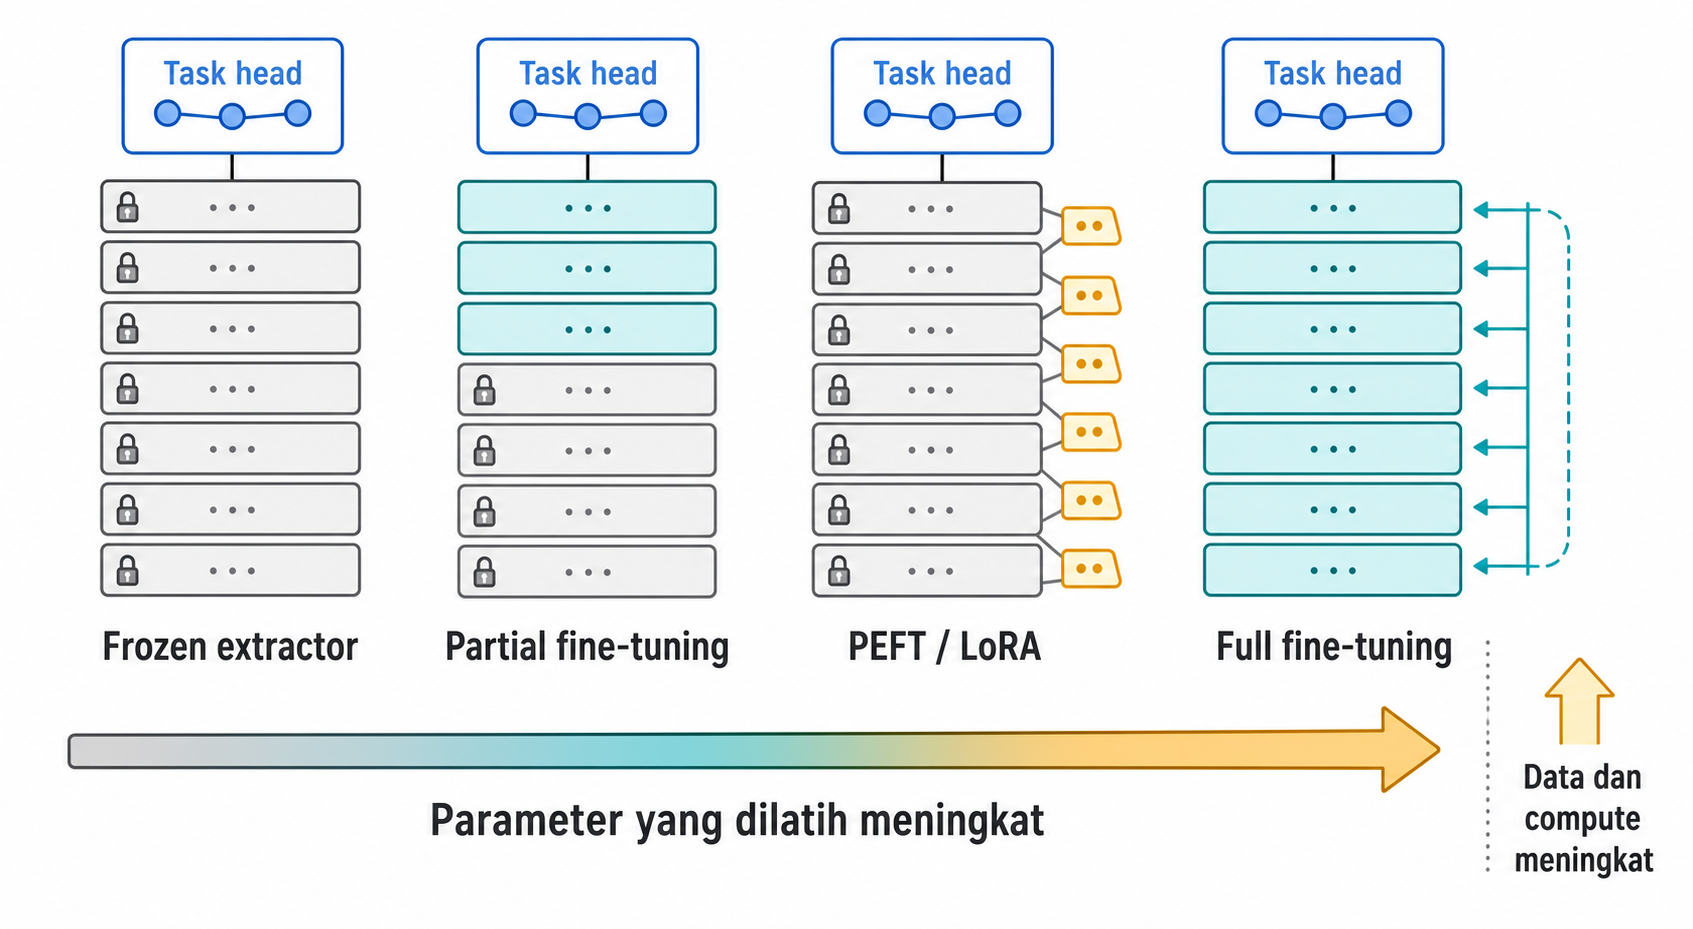
\includegraphics[width=\linewidth,height=0.72\textheight,keepaspectratio]{ch15-fig-1}
\caption{Spektrum Adaptasi Model Pretrained: Frozen Extractor, Partial, PEFT, Full Fine-Tuning}
\label{fig:ch15-fig-1}
\end{figure}

Secara matematis, prediksi model pada tugas baru diformulasikan sebagai fungsi komposit dari pengekstraksi fitur \emph{pretrained} \(g_\phi\) dan lapisan klasifikasi baru \(f_\theta\). Optimasi model dilakukan dengan meminimalkan fungsi kerugian, misalnya \emph{Cross-Entropy} (\(\mathcal{L}\)), terhadap data latih berukuran \(N\):

\[ \min_{\theta, \phi} \sum_{i=1}^{N} \mathcal{L}(y_i, f_\theta(g_\phi(x_i))) \]

Di mana \(x_i\) adalah input, \(y_i\) adalah label, \(\phi\) mewakili bobot model \emph{pretrained}, dan \(\theta\) merupakan bobot lapisan klasifikasi. Pendekatan adaptasi ditentukan oleh perlakuan terhadap parameter \(\phi\) selama proses optimasi. Spektrum ini memiliki empat titik utama:

\begin{enumerate}
\def\labelenumi{\arabic{enumi}.}
\tightlist
\item
  \textbf{Frozen Extractor}
  Pendekatan ini mengunci seluruh bobot model \emph{pretrained} sehingga parameter tidak berubah (\(\Delta\phi = 0\)). Model berfungsi secara kaku sebagai pengekstraksi fitur statis. Vektor \emph{embedding} yang keluar dari lapisan model digunakan untuk melatih algoritma pendamping, sehingga hanya parameter \(\theta\) yang diperbarui.
\end{enumerate}

\begin{itemize}
\tightlist
\item
  \textbf{Karakteristik:} Sangat efisien secara waktu dan komputasi. Pendekatan ini juga tahan terhadap \emph{overfitting} saat jumlah \emph{dataset} terbatas. Contoh terapannya adalah pemakaian ResNet beku untuk mengekstrak fitur visual dari gambar rontgen medis.
\end{itemize}

\begin{enumerate}
\def\labelenumi{\arabic{enumi}.}
\setcounter{enumi}{1}
\tightlist
\item
  \textbf{Partial Fine-Tuning}
  Strategi ini membuka beberapa lapisan terakhir dari model \emph{pretrained} untuk diperbarui, sedangkan lapisan awalnya dibiarkan terkunci.
\end{enumerate}

\begin{itemize}
\tightlist
\item
  \textbf{Karakteristik:} Memberikan titik keseimbangan komputasi dan akurasi. Lapisan awal tetap mempertahankan pengetahuannya dalam mendeteksi fitur fundamental, sementara lapisan akhir diizinkan beradaptasi menangkap pola spesifik pada \emph{dataset} baru.
\end{itemize}

\begin{enumerate}
\def\labelenumi{\arabic{enumi}.}
\setcounter{enumi}{2}
\tightlist
\item
  \textbf{Parameter-Efficient Fine-Tuning (PEFT)}
  Mengingat arsitektur model yang kian masif, pembaruan seluruh bobot menjadi sangat lambat dan mahal. PEFT, seperti metode LoRA (\emph{Low-Rank Adaptation}), mengunci bobot utama \(\phi\) dan menginjeksi matriks berukuran sangat kecil yang dapat dilatih ke dalam arsitektur model.
\end{enumerate}

\begin{itemize}
\tightlist
\item
  \textbf{Karakteristik:} Menghasilkan performa setara \emph{full fine-tuning} dengan melatih sebagian kecil parameter saja (sering kali di bawah 1\% dari total parameter asli). Metode ini menjadi standar industri adaptasi model besar sejak tahun 2024.
\end{itemize}

\begin{enumerate}
\def\labelenumi{\arabic{enumi}.}
\setcounter{enumi}{3}
\tightlist
\item
  \textbf{Full Fine-Tuning}
  Setiap lapisan model dibuka dan seluruh bobot parameternya (\(\phi\) dan \(\theta\)) diperbarui secara bersamaan mengikuti spesifikasi \emph{dataset} target.
\end{enumerate}

\begin{itemize}
\tightlist
\item
  \textbf{Karakteristik:} Menawarkan kapasitas representasi model yang maksimal, namun menguras banyak daya perangkat keras. Pendekatan ini mendatangkan risiko \emph{catastrophic forgetting}, yaitu kondisi saat model kehilangan pengetahuan umum asalnya akibat beradaptasi terlalu spesifik pada rentang data baru.
\end{itemize}

\section{Penyimpanan Embedding dan Metrik Kemiripan}\label{penyimpanan-embedding-dan-metrik-kemiripan}

Setelah representasi diekstraksi dari model \emph{pretrained} atau melalui proses \emph{fine-tuning}, representasi tersebut membutuhkan penyimpanan dan mekanisme perbandingan yang efisien. Sebuah vektor \emph{embedding} tunggal tidak bermakna tanpa konteks vektor lainnya. Vektor berdimensi tinggi ini disimpan di dalam \emph{feature bank} (sering disebut basis data vektor), yang dirancang khusus untuk menangani pencarian kemiripan.

Penerapan \emph{feature bank} di lingkungan produksi memiliki beberapa karakteristik operasional:

\begin{itemize}
\tightlist
\item
  \textbf{Kapasitas skala besar:} Mampu mengindeks dan menyimpan jutaan hingga miliaran vektor secara bersamaan.
\item
  \textbf{Pencarian sub-linear:} Sistem menghindari pemindaian setiap vektor satu per satu. Pendekatan yang dipakai adalah pemanfaatan struktur indeks kompresi, seperti \emph{Inverted File Index} atau \emph{Product Quantization}, guna mempercepat penemuan tetangga terdekat.
\item
  \textbf{Pustaka standar industri:} Implementasi seperti FAISS (Facebook AI Similarity Search) bertindak sebagai mesin pencari utama. FAISS menjembatani pembuatan \emph{embedding} dari model (misalnya \emph{sentence-transformers}) dengan sistem pencarian waktu nyata.
\end{itemize}

\begin{figure}[htbp]\centering
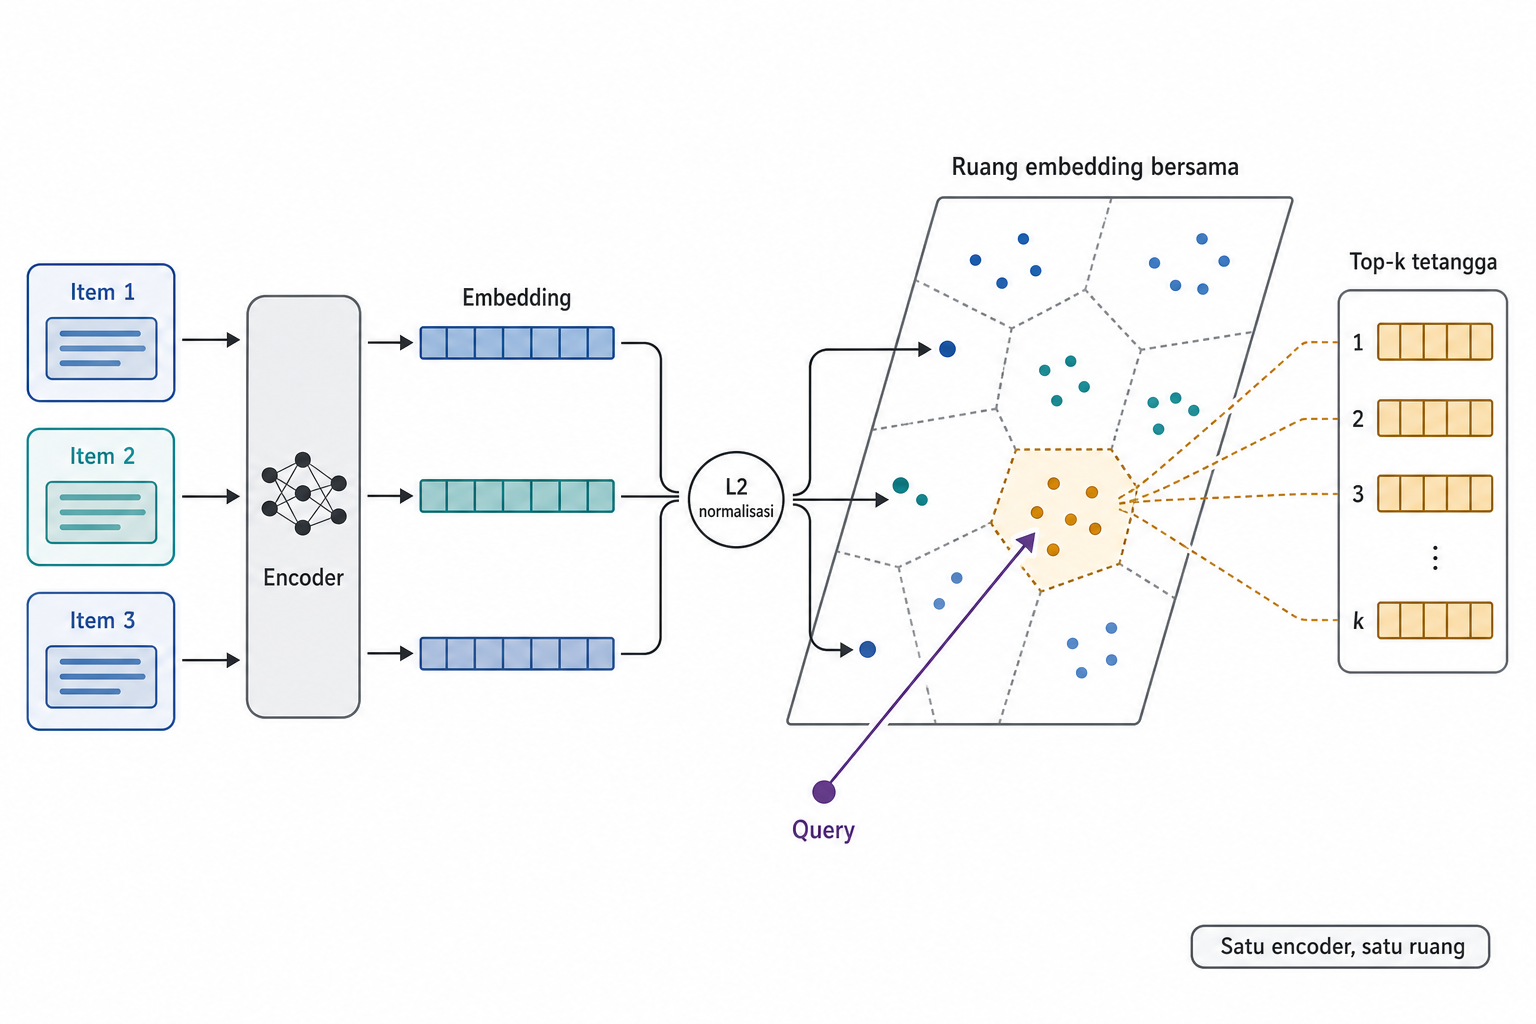
\includegraphics[width=\linewidth,height=0.72\textheight,keepaspectratio]{ch15-fig-2}
\caption{Alur Kerja Feature Bank Menggunakan Indeks FAISS}
\label{fig:ch15-fig-2}
\end{figure}

Untuk menentukan arti ``paling mirip'' dalam ruang berdimensi tinggi, sistem memakai metrik kemiripan. Metrik ini mendefinisikan cara perhitungan jarak antara dua vektor. Pada \emph{representasi yang dipelajari mesin} untuk teks atau citra, metrik yang dominan adalah \emph{cosine similarity}.

Metrik ini mengukur kosinus sudut antara dua vektor tanpa memedulikan panjang (magnitudo) vektor, dengan formulasi:

\[
\text{Cosine Similarity}(\mathbf{u}, \mathbf{v}) = \frac{\mathbf{u} \cdot \mathbf{v}}{\|\mathbf{u}\| \|\mathbf{v}\|}
\]

Pada persamaan tersebut, \(\mathbf{u}\) dan \(\mathbf{v}\) adalah dua vektor \emph{embedding} berdimensi \(d\) yang diukur kemiripannya, \(\mathbf{u} \cdot \mathbf{v}\) adalah \emph{dot product} (perkalian titik) keduanya, sedangkan \(\|\mathbf{u}\|\) dan \(\|\mathbf{v}\|\) adalah norma L2 (panjang atau magnitudo) masing-masing vektor.

Pemilihan metrik jarak biasanya menimbang tiga pendekatan berikut, sesuai arsitektur dan jenis data:

\begin{enumerate}
\def\labelenumi{\arabic{enumi}.}
\tightlist
\item
  \textbf{Cosine Similarity:} Mengabaikan panjang vektor dan hanya melihat arah orientasi. Pendekatan ini sangat tangguh untuk membedakan kemiripan semantik murni. Dua dokumen dengan pembahasan identik akan menghasilkan arah vektor yang searah, meski salah satu dokumen berukuran jauh lebih panjang.
\item
  \textbf{Dot Product:} Alternatif yang jauh lebih ringan secara komputasi karena membuang proses pembagian magnitudo. Jika seluruh vektor \(\mathbf{u}\) dan \(\mathbf{v}\) di dalam basis data telah dinormalisasi L2 (memiliki panjang tepat satu), perhitungan \emph{dot product} menjadi identik secara matematis dengan \emph{cosine similarity}. Menormalisasi vektor di awal merupakan praktik standar untuk meminimalkan beban komputasi saat melayani kueri berskala masif.
\item
  \textbf{Jarak Euclidean (L2 Distance):} Menghitung jarak garis lurus aktual antara dua koordinat titik. Berbeda dengan dua metrik sebelumnya, jarak Euclidean sensitif terhadap magnitudo vektor. Metrik ini digunakan jika intensitas ukuran fitur memiliki arti langsung, tetapi kurang ideal untuk membandingkan \emph{embedding} dari bidang pemrosesan bahasa alami (NLP) atau visi komputer.
\end{enumerate}

\section{Evaluasi Kualitas Embedding dan Risiko Domain Shift}\label{evaluasi-kualitas-embedding-dan-risiko-domain-shift}

Sebuah \emph{embedding} adalah pemetaan data ke ruang vektor. Namun, kualitas representasi ini sangat bergantung pada konteks tugas. Vektor yang memisahkan kelas dengan baik pada satu dataset bisa gagal total pada dataset lain. Hasil dari \emph{Massive Text Embedding Benchmark} (MTEB) mengonfirmasi bahwa tidak ada model \emph{embedding} tunggal yang mendominasi seluruh jenis tugas prediksi; setiap representasi memiliki keunggulan spesifik.

\textbf{Metode Linear Probing.}\label{metode-linear-probing}

Untuk mengevaluasi kualitas \emph{embedding} tanpa bias dari arsitektur klasifikasi yang rumit, kita menggunakan \emph{linear probing}. Metode ini memperlakukan model \emph{pretrained} murni sebagai ekstraktor fitur statis (\emph{frozen extractor}) dan menempatkan model linier sederhana di ujungnya.

Langkah pengujian ini mencakup:

\begin{itemize}
\tightlist
\item
  \textbf{Pembekuan parameter:} Seluruh bobot arsitektur model dikunci agar tidak berubah selama proses pelatihan tahap akhir.
\item
  \textbf{Ekstraksi representasi:} Data target dimasukkan ke model untuk menghasilkan vektor \emph{embedding} \(f(x_i)\).
\item
  \textbf{Pelatihan klasifikasi linier:} Sebuah pengklasifikasi sederhana (seperti regresi logistik) dilatih pada vektor tersebut.
\end{itemize}

Secara matematis, \emph{linear probing} mencari nilai matriks bobot linier \(W\) yang meminimalkan kerugian \emph{Cross-Entropy} pada klasifikasi klasifikasi multikelas:

\[ L(W) = -\frac{1}{N} \sum_{i=1}^{N} \sum_{c=1}^{C} y_{i,c} \log \left( \frac{\exp(W_c^T f(x_i))}{\sum_{k=1}^{C} \exp(W_k^T f(x_i))} \right) \]

Dalam persamaan tersebut, \(f(x_i)\) adalah representasi yang dipelajari mesin dengan parameter asal yang dibiarkan tetap (\emph{frozen}), \(W_c\) adalah vektor bobot lapisan klasifikasi untuk kelas \(c\), dan \(y_{i,c}\) bernilai 1 jika sampel \(i\) berada di kelas \(c\) serta 0 jika tidak.

Jika model linier sederhana mampu meminimalkan fungsi kerugian ini dan meraih akurasi tinggi, model \emph{pretrained} terbukti sukses menyusun data dan memisahkan kelas target di ruang vektor. Sebaliknya, jika akurasi tinggi baru didapat setelah kita mengganti model linier dengan algoritma non-linier yang lebih rumit, berarti representasi dasar tersebut gagal menstrukturkan data dengan baik.

\begin{figure}[htbp]\centering
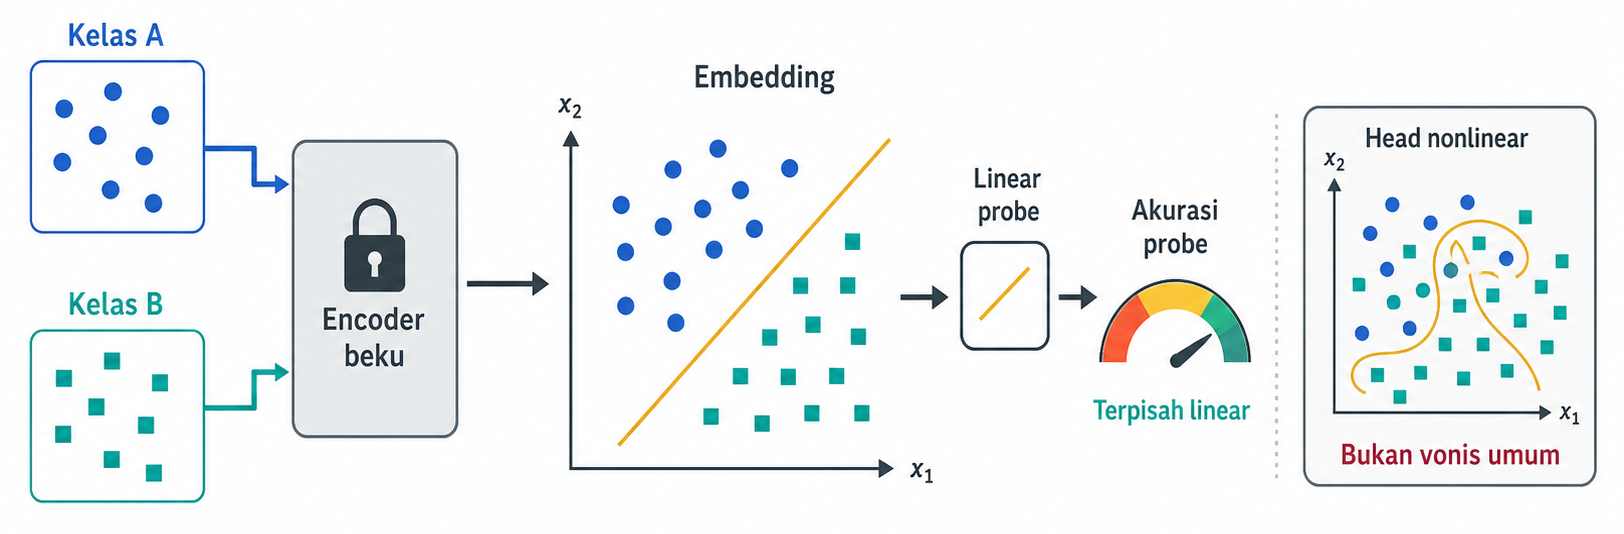
\includegraphics[width=\linewidth,height=0.72\textheight,keepaspectratio]{ch15-fig-3}
\caption{Arsitektur Linear Probing}
\label{fig:ch15-fig-3}
\end{figure}

\textbf{Mengidentifikasi Domain Shift.}\label{mengidentifikasi-domain-shift}

Transfer representasi dari luar kerap menemui jalan buntu akibat \emph{domain shift} - perbedaan fundamental antara sebaran data tempat model \emph{pretrained} dilatih dengan data tugas akhir kita. Model membawa asumsi bentuk data dari proses pelatihannya; saat asumsi ini dilanggar, representasi yang dihasilkan kehilangan makna.

Kondisi \emph{domain shift} menimbulkan dampak beruntun dalam \emph{pipeline}:

\begin{itemize}
\tightlist
\item
  \textbf{Kebutaan terhadap fitur target:} Model visi yang dilatih membedakan hewan dan kendaraan tidak memiliki referensi tekstur untuk mengurai patologi citra medis (seperti rontgen paru-paru).
\item
  \textbf{Tumpang-tindih representasi:} Akibat gagal mendeteksi pola yang relevan, model memetakan gambar rontgen pasien sehat dan sakit ke koordinat vektor yang berdekatan atau bertumpuk.
\item
  \textbf{Degradasi fungsi prediktif:} Karena ruang vektor gagal memisahkan konsep yang berbeda, model klasifikasi akhir tidak memiliki fitur diskriminatif untuk dipelajari.
\end{itemize}

Ketika \emph{domain shift} terlalu tajam, arsitektur \emph{frozen extractor} tidak lagi memadai. Praktisi perlu menggeser strategi menjauhi pembekuan total dan mulai melakukan \emph{fine-tuning} parsial maupun menyeluruh. Pembaruan bobot ini secara langsung memaksa jaringan saraf menyesuaikan diri untuk mempelajari struktur dan distribusi khusus dari dataset target yang baru.

\section{Batas Konseptual: Transfer Representasi vs.~Kompresi Data Internal}\label{batas-konseptual-transfer-representasi-vs.-kompresi-data-internal}

Representasi laten hasil reduksi dimensi (seperti yang dibahas pada Bab 8) dan \emph{embedding} dari \emph{pre-trained model} sering dianggap serupa karena keduanya memetakan input berdimensi tinggi menjadi vektor berdimensi rendah. Perbedaan fundamental di antara keduanya terletak pada sumber pengetahuan yang membentuk representasi tersebut.

Pendekatan ini dapat dibedakan berdasarkan asal datanya:

\begin{itemize}
\tightlist
\item
  \textbf{Kompresi Data Internal:} Metode seperti PCA, SVD, atau \emph{autoencoder} beroperasi secara murni pada himpunan data lokal. Teknik ini menemukan sumbu variasi dan melipat redundansi dari dalam matriks fitur itu sendiri. Representasi akhirnya dibentuk sepenuhnya oleh pola observasi lokal, tanpa tambahan informasi eksternal.
\item
  \textbf{Transfer Representasi Eksternal:} \emph{Pre-trained model} mentransfer struktur makna dari jutaan data eksternal ke dalam masalah prediksi spesifik. Model ini membawa pemahaman abstrak - seperti relasi semantik teks atau hierarki fitur visual - yang tidak mungkin dipelajari secara kokoh dari dataset lokal yang sempit.
\end{itemize}

Batas kedua kategori ini bukanlah perbedaan ``metode statistik vs.~Jaringan saraf tiruan''. Sebuah \emph{autoencoder} berarsitektur \emph{deep learning} tetap beroperasi sebagai alat kompresi internal jika dilatih dari awal hanya menggunakan data proyek terkait. Pembeda utamanya terletak pada asal representasi: apakah algoritma memadatkan data target itu sendiri, atau mentransfer pengetahuan dari luar.

\begin{figure}[htbp]\centering
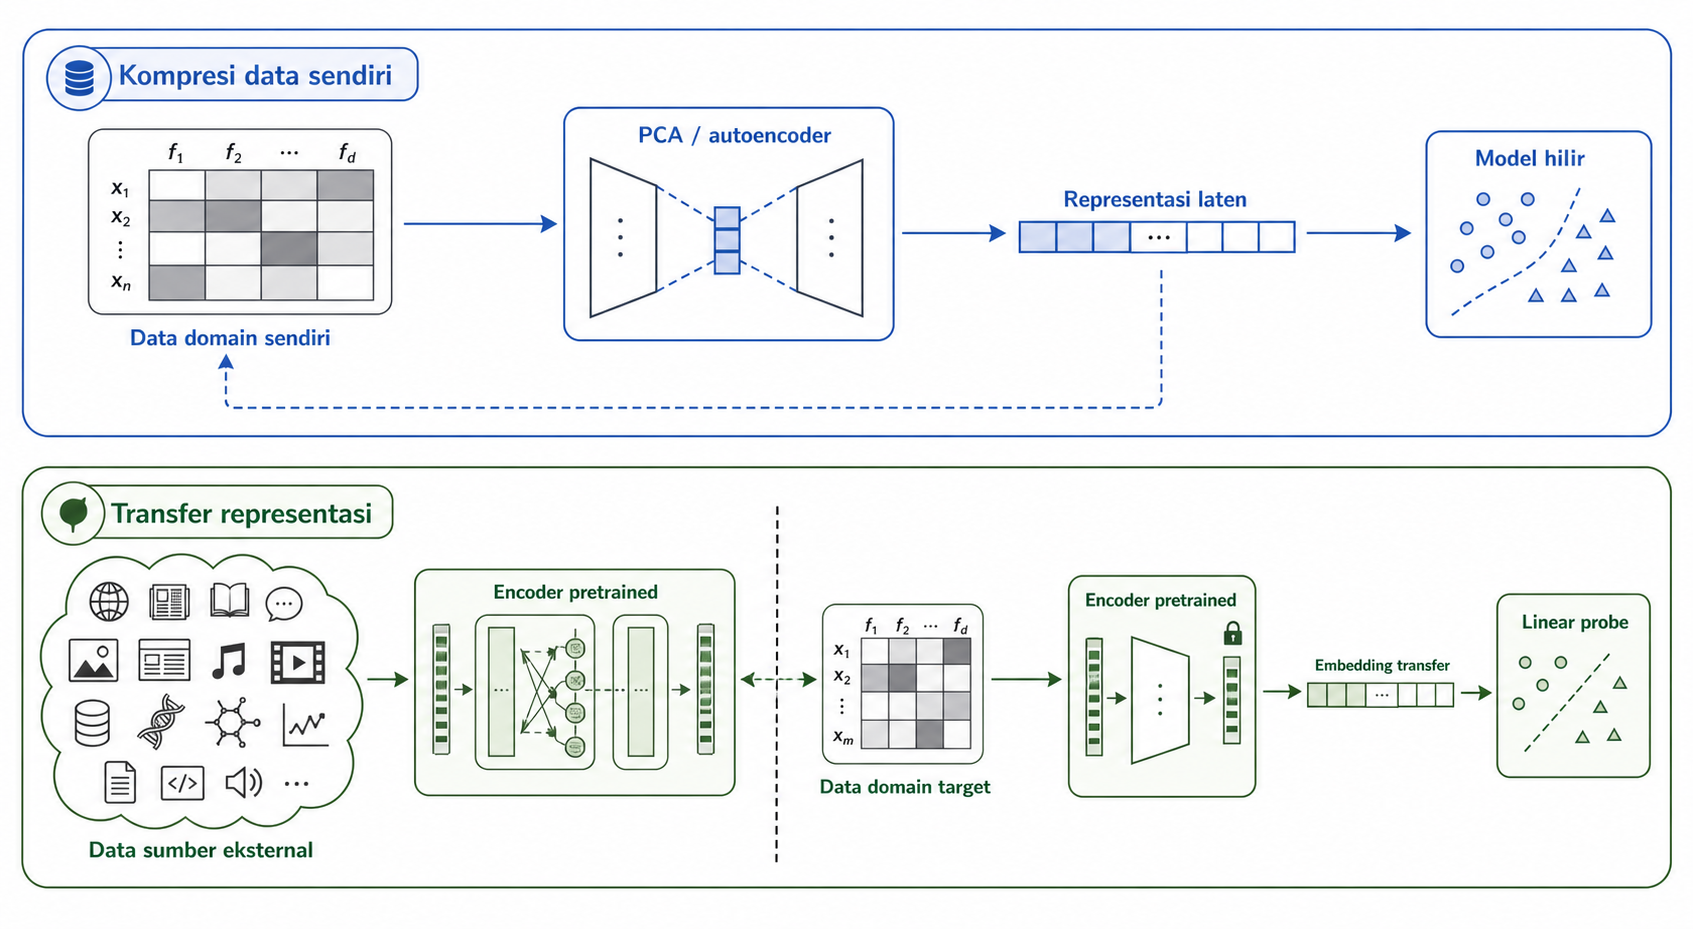
\includegraphics[width=\linewidth,height=0.72\textheight,keepaspectratio]{ch15-fig-4}
\caption{Skema Transfer Learning (Membekukan Layer)}
\label{fig:ch15-fig-4}
\end{figure}

Secara matematis, perbedaan tersebut terlihat dari fungsi objektif yang digunakan saat melatih pembentuk representasi. Pada transfer representasi, \emph{pre-trained model} umumnya dioptimalkan lebih dulu untuk tugas klasifikasi eksternal (misalnya membedakan kelas objek pada ImageNet) menggunakan fungsi kerugian \emph{Cross-Entropy}:

\[ \mathcal{L}_{CE} = - \sum_{i=1}^{C} y_i \log(\hat{y}_i) \]

Dalam persamaan tersebut, \(C\) adalah jumlah total kelas target pada dataset eksternal, \(y_i\) adalah label kelas aktual sebuah observasi, dan \(\hat{y}_i\) adalah probabilitas prediksi yang dihasilkan model.

Bobot jaringan yang telah mengoptimalkan \(\mathcal{L}_{CE}\) pada distribusi eksternal tersebut kemudian dibekukan (\emph{frozen}) dan digunakan sebagai ekstraktor fitur tetap untuk masalah lokal. Konsep ini berbeda dengan kompresi internal yang meminimalkan fungsi kerugian rekonstruksi (seperti \emph{mean squared error} pada \emph{autoencoder}) tanpa mengandalkan label klasifikasi dari luar \emph{pipeline}.

Pemisahan kompresi dan transfer membawa konsekuensi teknis pada perancangan \emph{pipeline}:

\begin{itemize}
\tightlist
\item
  \textbf{Kapasitas Pembelajaran:} Ekstraksi fitur dari luar menjadi solusi utama ketika dataset pelatihan terlalu kecil untuk membentuk matriks representasi sendiri.
\item
  \textbf{Risiko \emph{Domain Shift}:} \emph{Pre-trained model} berisiko mengalami pergeseran domain jika distribusi asli pelatihannya jauh meleset dari konteks prediksi akhir (misalnya \emph{embedding} bahasa umum diterapkan pada dokumen legal). Kompresi internal terhindar dari risiko ini karena fondasinya dibangun langsung di atas distribusi target.
\end{itemize}

\section{Apakah Deep Learning Menghapus Kebutuhan Rekayasa Fitur?}\label{apakah-deep-learning-menghapus-kebutuhan-rekayasa-fitur}

Banyak praktisi pemula berpandangan bahwa \emph{deep learning} telah menggantikan peran rekayasa fitur secara keseluruhan. Jaringan saraf tiruan memang mampu mengekstraksi pola rumit secara otomatis dari data mentah. Kemampuan ini sering memunculkan asumsi bahwa campur tangan manusia tidak lagi dibutuhkan. Namun, \emph{deep learning} tidak menghilangkan rekayasa fitur, melainkan sekadar menggeser ranah fokusnya.

Model \emph{deep learning} sangat unggul dalam membentuk representasi yang dipelajari mesin. Keunggulan ini terlihat paling jelas ketika algoritma memproses data tidak terstruktur seperti kumpulan teks, citra, atau gelombang audio. Meskipun algoritma mampu mengekstrak pola padat dari data mentah, sistem komputasi tidak dapat merumuskan masalah prediksinya sendiri. Keputusan fundamental terkait penyusunan data tetap berada di tangan perancang manusia. Beberapa keputusan utama meliputi:

\begin{itemize}
\tightlist
\item
  \textbf{Penentuan unit observasi:} Mendefinisikan secara pasti batas satu sampel data observasi tunggal.
\item
  \textbf{Definisi variabel target:} Menetapkan label yang harus diprediksi beserta horizon waktu yang relevan.
\item
  \textbf{Konstruksi arsitektur masukan:} Menyusun aliran informasi agar jaringan saraf dapat mencernanya secara maksimal.
\end{itemize}

Praktik rekayasa fitur telah beralih dari kalkulasi transformasi matematis eksplisit untuk setiap variabel tunggal menuju injeksi bias induktif. Representasi yang dirancang manusia berguna untuk memasukkan pengetahuan pakar ke dalam model. Aturan logika bisnis spesifik, batasan fisika lingkungan nyata, maupun formula baku rasio keuangan merupakan contoh pola yang sulit dipelajari murni dari probabilitas data.

\begin{figure}[htbp]\centering
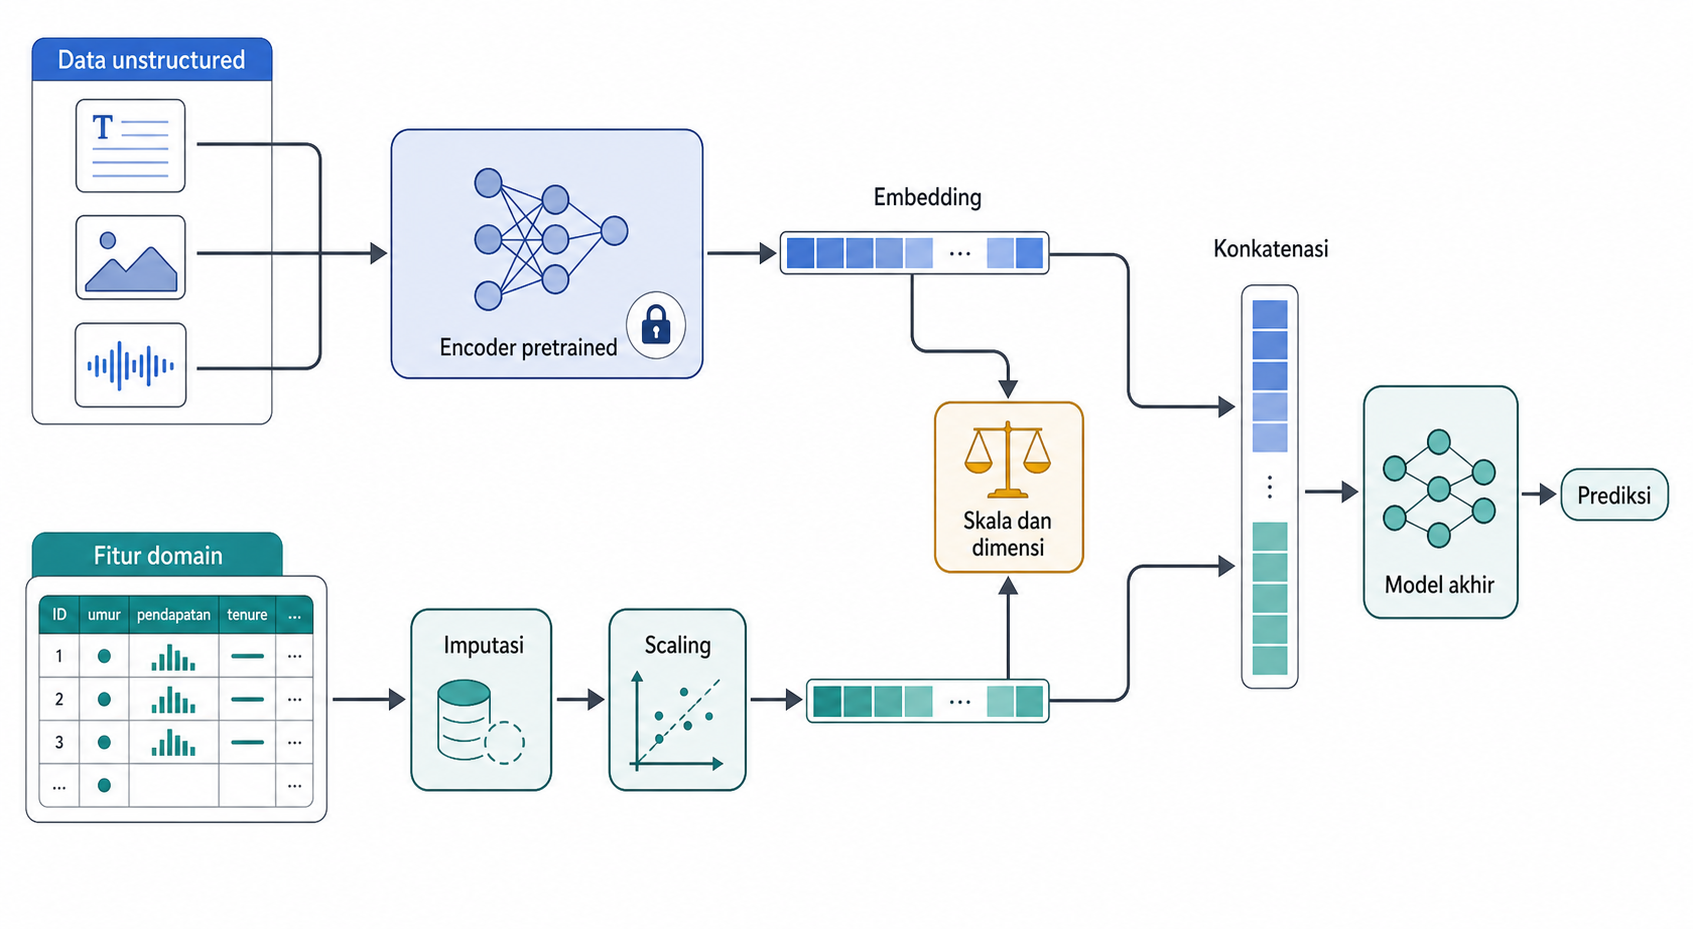
\includegraphics[width=\linewidth,height=0.72\textheight,keepaspectratio]{ch15-fig-5}
\caption{Perbandingan Arsitektur Fine-Tuning Penuh dengan Feature Extraction Beku}
\label{fig:ch15-fig-5}
\end{figure}

Dalam proses pelatihannya, jaringan saraf berfokus menyesuaikan parameter untuk meminimalkan penyimpangan prediksi. Sebagai contoh, pembaruan \emph{pre-trained weights} dalam tugas klasifikasi multikelas umumnya menggunakan fungsi kerugian \emph{cross-entropy}:

\[ \mathcal{L} = -\frac{1}{N} \sum_{i=1}^{N} \sum_{c=1}^{C} y_{i,c} \log(\hat{y}_{i,c}) \]

Di mana \(\mathcal{L}\) melambangkan nilai total fungsi kerugian, \(N\) adalah jumlah sampel latih, \(C\) merepresentasikan jumlah kelas target, \(y_{i,c}\) menyatakan probabilitas aktual kelas (\emph{ground truth}), dan \(\hat{y}_{i,c}\) adalah probabilitas prediksi keluaran model.

Representasi yang dirancang manusia menuntun algoritma agar proses penurunan nilai \(\mathcal{L}\) tidak membuang kapasitas model untuk mencari pola yang sebenarnya sudah diketahui kebenarannya. Tanpa panduan tersebut, model rentan menghafal gangguan acak (\emph{noise}), terlebih ketika pasokan data latih sangat terbatas.

Pergeseran peran rekayasa fitur semakin meluas seiring penggunaan model bahasa besar (LLM). Dua praktik terbaru membuktikan bahwa rekayasa fitur berubah bentuk:

\begin{itemize}
\tightlist
\item
  \textbf{Ekstraksi fitur berbasis \emph{prompting}:} Memanfaatkan LLM untuk menarik struktur dari teks tidak terstruktur, seperti klasifikasi sentimen atau daftar entitas. Hasil ekstraksi ini kemudian dipasok sebagai fitur untuk model prediksi lain.
\item
  \textbf{\emph{Retrieval-Augmented Generation} (RAG):} Mengambil dokumen eksternal untuk melengkapi ruang konteks suatu \emph{prompt}. Praktik ini setara dengan metode rekayasa fitur dinamis, karena dokumen hasil penelusuran beroperasi sebagai representasi berdimensi tinggi yang memperbaiki pemahaman konteks model.
\end{itemize}

Pendekatan menggunakan representasi yang dirancang manusia maupun representasi yang dipelajari mesin harus dipandang sebagai dua entitas yang saling melengkapi. Manusia bertugas membingkai batasan dan logika domain, sementara mesin mengeksplorasi pola tersembunyi pada dimensi tinggi. Kemitraan ini menghasilkan \emph{pipeline} pembelajaran yang tangguh dan dapat diandalkan pada berbagai skenario nyata.

\section{Representasi Input: Tokenisasi dan Augmentasi Data}\label{representasi-input-tokenisasi-dan-augmentasi-data}

Rekayasa fitur tidak hilang di era \emph{deep learning}. Jaringan saraf tidak memproses teks, gelombang suara, atau cahaya secara langsung; model hanya menerima matriks angka. Proses menerjemahkan data mentah menjadi format numerik ini tetap dirancang oleh manusia dan menjadi prasyarat sebelum model mulai belajar.

Beberapa praktik rekayasa fitur konvensional yang tetap bertahan dalam \emph{pipeline} model modern meliputi:

\begin{itemize}
\tightlist
\item
  \textbf{Tokenisasi teks:} Kita perlu memecah rentetan karakter menjadi unit diskret. Pendekatan berbasis \emph{subword} seperti \emph{Byte-Pair Encoding} (BPE) memecah kata kompleks menjadi fragmen yang lebih kecil. Metode ini membatasi ukuran kosakata model sekaligus membantu mesin mengenali makna dari potongan kata. Pada tahap ini, token khusus sering ditambahkan untuk merangkum konteks kalimat.
\end{itemize}

\begin{figure}[htbp]\centering
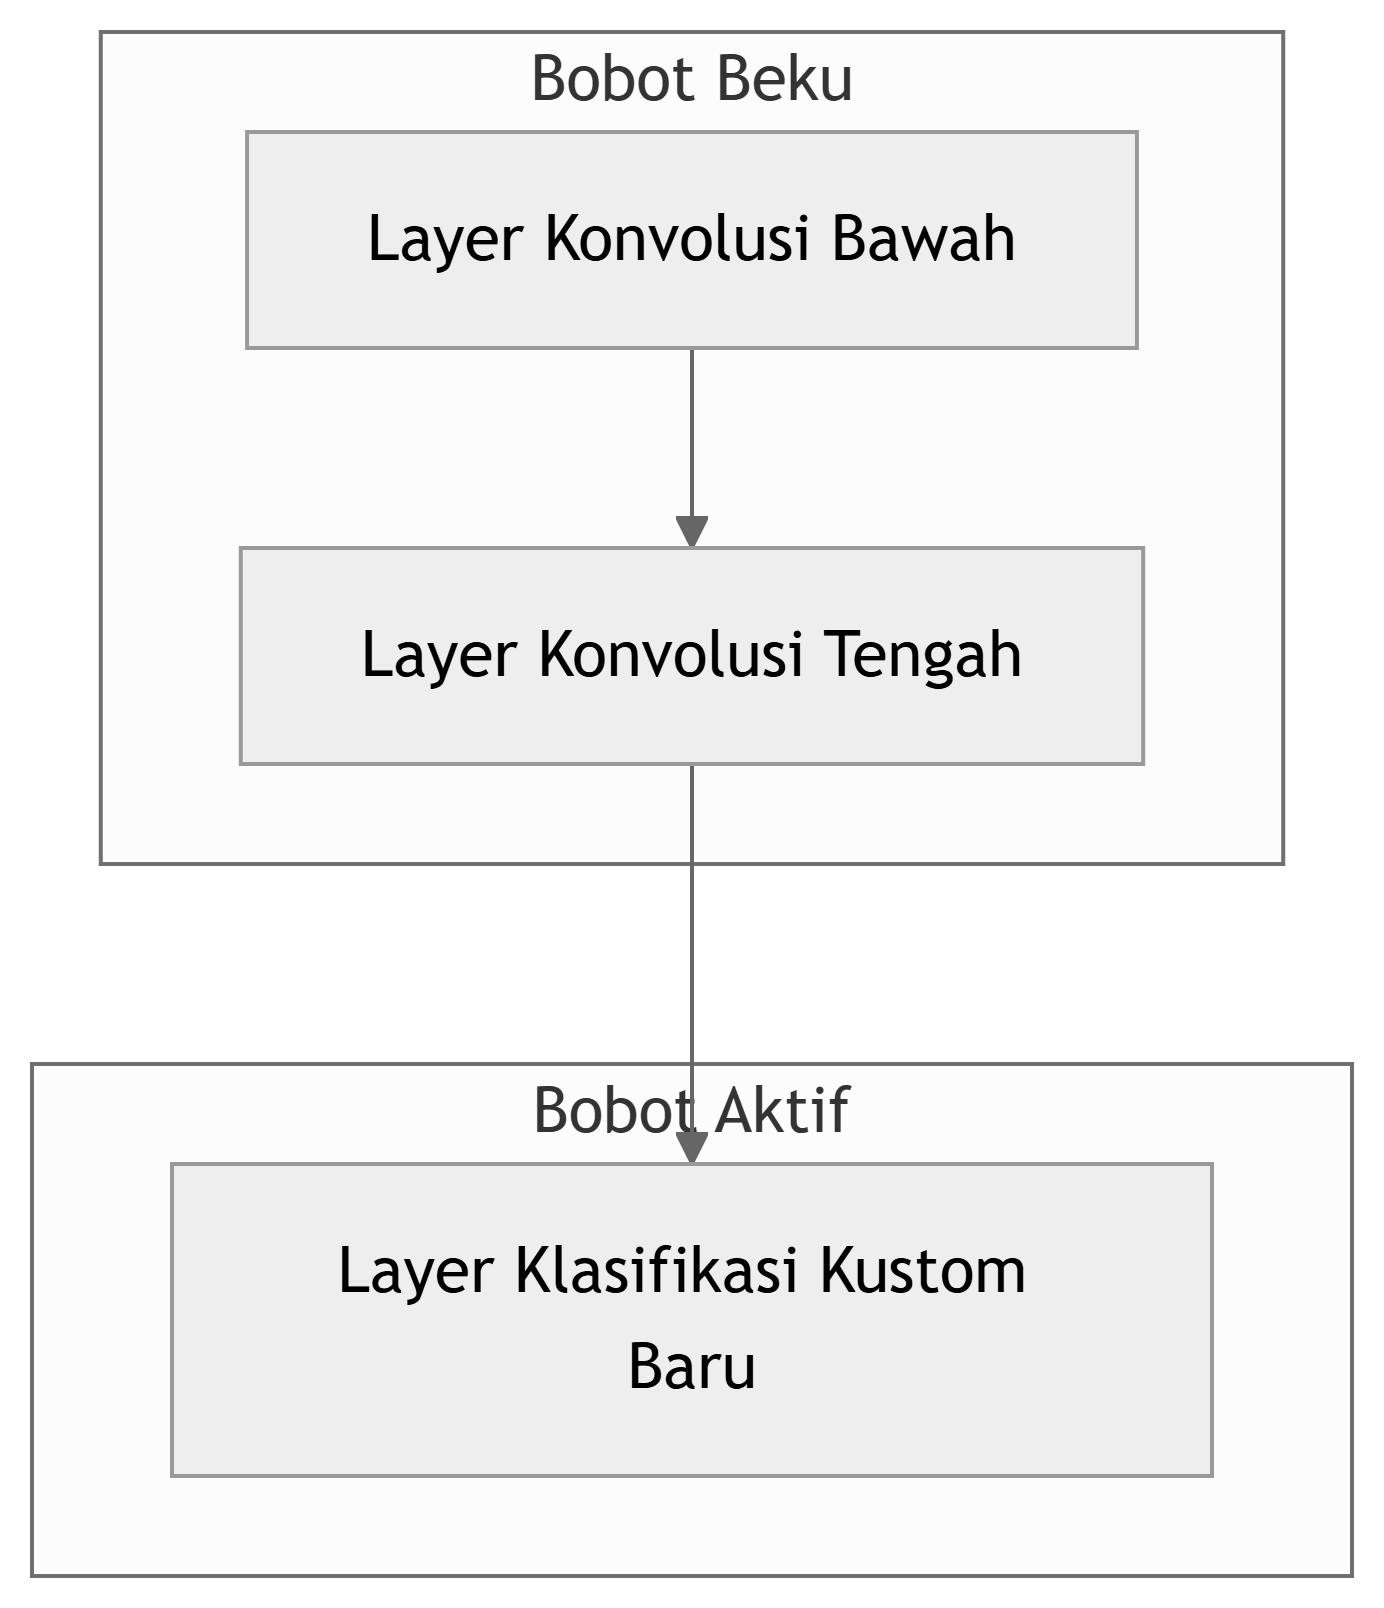
\includegraphics[width=\linewidth,height=0.72\textheight,keepaspectratio]{ch15-fig-6}
\caption{Ekstraksi CLS Token dari Transformer untuk Menghasilkan Embedding Tunggal}
\label{fig:ch15-fig-6}
\end{figure}

\begin{itemize}
\tightlist
\item
  \textbf{Augmentasi data:} Praktik ini menambahkan variasi buatan ke dalam data latih. Pada pengolahan citra, kita sering membalik gambar, menggeser piksel, atau mengubah kecerahan warnanya. Modifikasi ini menanamkan pengetahuan domain dan mencegah model hanya menghafal posisi objek.
\item
  \textbf{Normalisasi fitur numerik:} Jaringan saraf sensitif terhadap perbedaan skala \emph{input}. Jika satu fitur berada di rentang ribuan sementara fitur lain berupa pecahan desimal, turunan (\emph{gradient}) dari fungsi kerugian menjadi tidak proporsional. Dalam tugas klasifikasi, pembaruan bobot model dievaluasi menggunakan fungsi \emph{Cross-Entropy}:
\end{itemize}

\[ L = - \sum_{c=1}^{C} y_c \log(\hat{y}_c) \]

Di mana \(L\) adalah nilai kerugian, \(C\) adalah jumlah kelas target, \(y_c\) adalah label sebenarnya, dan \(\hat{y}_c\) adalah probabilitas prediksi dari model. Skala \emph{input} mentah yang ekstrem akan mengacaukan perhitungan turunan dari persamaan ini dan menghambat konvergensi jaringan.

Langkah-langkah tersebut memperlihatkan bagaimana rekayasa konvensional hanya bergeser posisi. Transformasi awal ini adalah bentuk representasi yang dirancang manusia. Manusia menyiapkan batasan dan struktur \emph{input} yang terukur, yang selanjutnya berfungsi sebagai fondasi bagi model untuk mengekstraksi representasi yang dipelajari mesin pada lapisan-lapisan berikutnya.

\section{\texorpdfstring{\emph{Deep Learning} pada Data Tabular: Mempelajari Embedding Terstruktur}{Deep Learning pada Data Tabular: Mempelajari Embedding Terstruktur}}\label{deep-learning-pada-data-tabular-mempelajari-embedding-terstruktur}

Algoritma berbasis pohon seperti \emph{gradient boosting} telah lama menjadi pilihan utama untuk data \emph{tabular}. Kini, \emph{deep learning} menawarkan pendekatan yang berbeda: mempelajari representasi vektor secara langsung dari tabel. Jika Bab 4 menggunakan \emph{entity embedding} khusus untuk variabel kategorikal, \emph{deep tabular learning} memperluas perlakuan ini ke seluruh baris. Tujuannya adalah memetakan fitur kategorikal dan numerik ke dalam ruang vektor yang seragam, sehingga model dapat menyatukannya menjadi satu representasi utuh.

\textbf{Arsitektur dan Tokenisasi Fitur}

Arsitektur modern seperti FT-Transformer dan TabNet mengadaptasi mekanisme \emph{attention} dari pemrosesan bahasa alami untuk membaca baris data. Alih-alih melihat baris sebagai rentetan skalar statis, model memperlakukan setiap nilai fitur sebagai sebuah token independen.

Agar dapat diproses bersama, setiap nilai numerik dan kategorikal harus diubah menjadi \emph{embedding} dengan dimensi yang sama. Untuk fitur kategorikal, model menggunakan \emph{lookup table} standar. Untuk fitur numerik \(j\) dengan nilai skalar \(x_j\), transformasi linear (tokenisasi numerik) dilakukan melalui persamaan:

\[ T_{num}^{(j)} = \mathbf{w}_j x_j + \mathbf{b}_j \]

Dalam persamaan tersebut, \(T_{num}^{(j)}\) adalah \emph{embedding} vektor padat untuk fitur numerik itu, \(\mathbf{w}_j\) adalah vektor bobot yang dipelajari mesin, \(\mathbf{b}_j\) adalah vektor bias, dan \(x_j\) adalah nilai skalar numerik aslinya.

Setelah tokenisasi, arsitektur \emph{transformer} menyisipkan token khusus (biasa disebut token \passthrough{\lstinline![CLS]!}) di awal barisan fitur. Lapisan \emph{attention} kemudian mempelajari interaksi antar-fitur. Token \passthrough{\lstinline![CLS]!} ini bertugas menghimpun informasi dari seluruh fitur lain untuk menjadi \emph{embedding} final dari baris data tersebut.

\begin{figure}[htbp]\centering
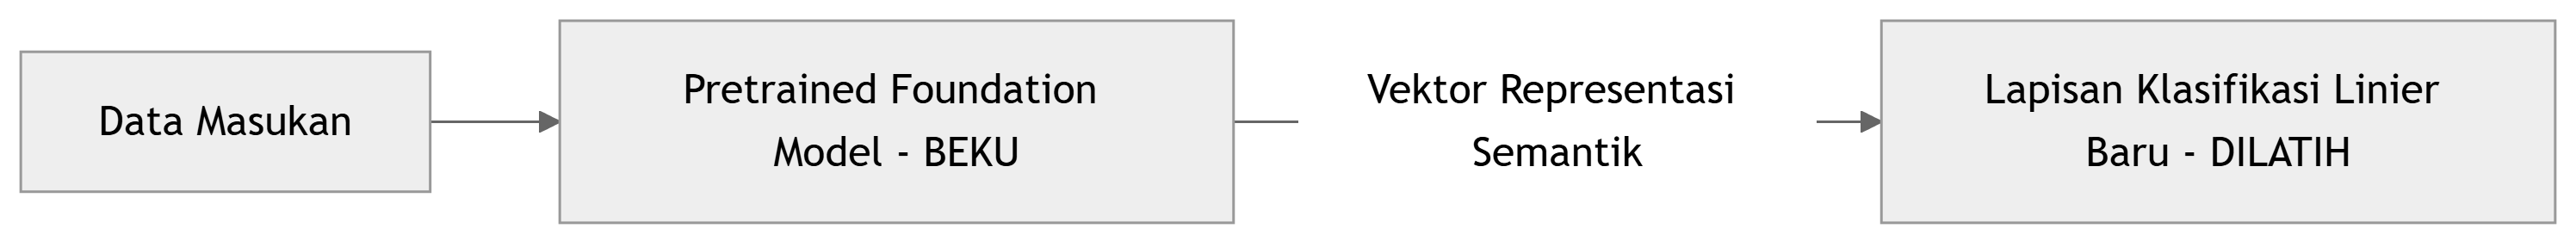
\includegraphics[width=\linewidth,height=0.72\textheight,keepaspectratio]{ch15-fig-7}
\caption{Arsitektur Model Hybrid yang Menggabungkan Fitur Rekayasa Tabular \& Vektor Embedding}
\label{fig:ch15-fig-7}
\end{figure}

\textbf{Ekstraksi Fitur dan \emph{Foundation Models}}

Berkat representasi seragam ini, model \emph{deep tabular} berfungsi sangat baik sebagai ekstraktor fitur. Vektor padat yang ditarik dari token \passthrough{\lstinline![CLS]!} merangkum seluruh variabel beserta relasinya. Vektor ini kemudian dapat diteruskan ke model prediksi hilir yang lebih ringan.

Riset terbaru pada rentang 2024--2025 bahkan mendorong pendekatan ini lebih jauh melalui \emph{tabular foundation models} seperti TabPFN. Arsitektur ini memanfaatkan \emph{in-context learning}, di mana model membaca kumpulan contoh data latih langsung di dalam \emph{prompt} memori tanpa memerlukan pembaruan bobot sama sekali. Terobosan ini menandai titik di mana data tabular mulai mendapatkan model prapelatih (\emph{pretrained}) yang mampu menggeneralisasi lintas dataset, sama seperti yang terjadi pada teks dan citra.

\textbf{Memilih Antara \emph{Deep Learning} dan \emph{Gradient Boosting}}

Meskipun sangat menjanjikan, \emph{deep learning} tabular tidak otomatis menggantikan algoritma pohon. Pemilihan metode sangat bergantung pada ukuran dan sifat data:

\begin{itemize}
\item
  \textbf{Pilih \emph{Gradient Boosting} (XGBoost, LightGBM, CatBoost) ketika:}
\item
  Volume data berada pada skala kecil hingga menengah (umumnya di bawah 50.000 baris).
\item
  Data memiliki variasi rentang nilai skalar yang ekstrem atau \emph{outlier} tebal (pemisahan pada algoritma pohon tidak sensitif terhadap skala fitur).
\item
  Tugas prediksi menuntut pembentukan batasan keputusan tak-linear tanpa penalaan parameter jaringan saraf yang rumit.
\item
  \textbf{Pilih \emph{Deep Tabular Learning} ketika:}
\item
  Dataset berukuran masif dan sistem produksi memerlukan pembaruan representasi secara berkelanjutan (\emph{incremental learning}).
\item
  Sistem menuntut ekstraksi representasi per baris (berupa \emph{embedding} padat) untuk digunakan ulang pada modul hilir.
\item
  Terdapat kebutuhan fusi multimodal. Representasi \emph{tabular} berbasis vektor dapat langsung digabungkan dengan representasi teks atau citra di dalam satu ruang arsitektur jaringan yang terintegrasi.
\end{itemize}

\section{Model Hybrid: Menggabungkan Fitur Rekayasa dan Embedding}\label{model-hybrid-menggabungkan-fitur-rekayasa-dan-embedding}

Sistem \emph{machine learning} tingkat produksi jarang menggunakan rekayasa fitur tabular atau representasi \emph{deep learning} secara eksklusif. Arsitektur \emph{hybrid} mengintegrasikan representasi yang dirancang manusia dengan representasi yang dipelajari mesin untuk mengoptimalkan sistem prediktif. Pendekatan ini menggabungkan keunggulan dari kedua jenis fitur:

\begin{itemize}
\tightlist
\item
  \textbf{Fitur rancangan manusia:} Menginjeksi batasan logika yang tegas, aturan bisnis absolut, dan ukuran matematika konkret (seperti agregasi waktu atau rasio finansial) yang sulit diinferensi secara mandiri oleh jaringan saraf.
\item
  \textbf{Representasi \emph{embedding}:} Mengekstraksi pola semantik dari data tidak terstruktur (citra, audio, atau teks panjang) yang mustahil dikodekan melalui aturan pemrograman manual.
\end{itemize}

\begin{figure}[htbp]\centering
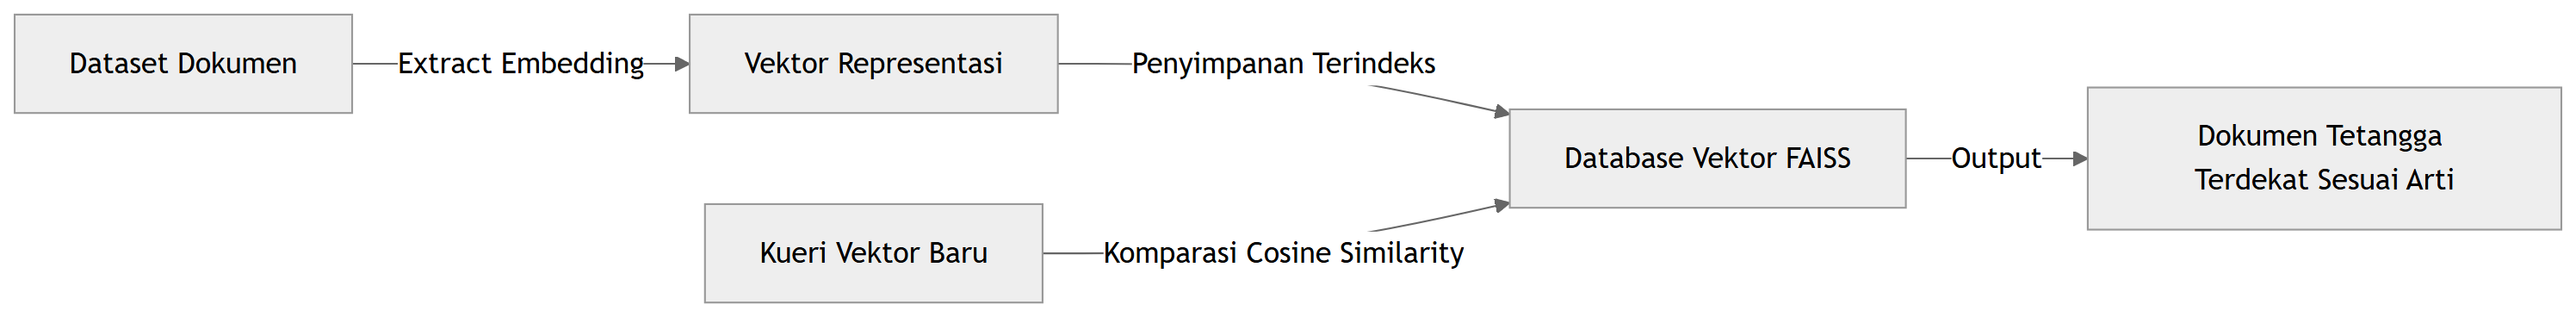
\includegraphics[width=\linewidth,height=0.72\textheight,keepaspectratio]{ch15-fig-8}
\caption{Arsitektur Integrasi Pipeline Hibrida Menggabungkan Teks Pretrained + Tabular}
\label{fig:ch15-fig-8}
\end{figure}

Secara struktural, penggabungan ini dilakukan melalui operasi konkatenasi vektor sebelum lapisan prediksi akhir. Vektor fitur tabular yang telah melewati tahap normalisasi dan pemrosesan awal disejajarkan dengan vektor \emph{embedding} dari ekstraktor model \emph{pretrained}.

Secara matematis, operasi fusi ini diformulasikan sebagai:

\[ \mathbf{x}_{hybrid} = [\mathbf{x}_{engineered} \parallel \mathbf{e}_{learned}] \]

Dalam persamaan tersebut, \(\mathbf{x}_{hybrid}\) adalah vektor gabungan akhir yang diteruskan ke algoritma klasifikasi atau regresi, \(\mathbf{x}_{engineered} \in \mathbb{R}^d\) adalah vektor fitur tabular rancangan manusia yang telah diskalakan, dan \(\mathbf{e}_{learned} \in \mathbb{R}^k\) adalah representasi padat dari model \emph{pretrained} (misalnya representasi \emph{bottleneck} pada ResNet atau token CLS pada Transformer). Notasi \(\parallel\) melambangkan operasi konkatenasi vektor.

Kasus pemodelan harga perumahan menggambarkan interaksi ini secara konkret. Model \emph{hybrid} memproses data melalui dua jalur paralel:

\begin{enumerate}
\def\labelenumi{\arabic{enumi}.}
\tightlist
\item
  \textbf{Jalur tidak terstruktur:} Model visi komputasi memproses fitur gambar untuk menghasilkan vektor \emph{embedding} dari sekumpulan foto interior rumah. Vektor ini mendeteksi variabel abstrak seperti estetika, pencahayaan alami, dan gaya arsitektur.
\item
  \textbf{Jalur tabular:} Sistem merekayasa data numerik dan kategorikal, seperti vektor spasial (jarak ke fasilitas transportasi), proporsi dimensi bangunan, dan usia properti.
\end{enumerate}

Bila beroperasi secara terpisah, \emph{embedding} visual tidak memiliki referensi tentang ukuran geografis maupun rasio spasial, sedangkan model regresi tabular mengabaikan diferensiasi estetika visual. Penggabungan vektor \(\mathbf{x}_{hybrid}\) menutupi kedua titik buta tersebut. Keseluruhan representasi gabungan ini kemudian diteruskan sebagai \emph{input} tambahan ke jaringan \emph{multilayer perceptron} (MLP) penutup atau digunakan dalam algoritma \emph{gradient boosting}, sehingga prediksi akhir model tetap terjangkar secara logis pada aturan metrik spesifik \emph{domain}.

\section{\texorpdfstring{Studi Kasus: \emph{Pretrained Extractor} dan Model \emph{Hybrid}}{Studi Kasus: Pretrained Extractor dan Model Hybrid}}\label{studi-kasus-pretrained-extractor-dan-model-hybrid}

Studi kasus prediksi pengembalian barang (\emph{product returns}) pada platform niaga digital sangat relevan untuk mengilustrasikan cara menyatukan seluruh konsep representasi ini ke dalam satu \emph{pipeline} prediktif yang solid. Sistem dituntut memproses dua sumber modalitas secara serentak: ulasan teks dari pelanggan dan riwayat transaksi tabular dari pelanggan yang bersangkutan. Karakteristik ganda ini dipecahkan melalui arsitektur \emph{hybrid} yang menyinergikan ekstraksi \emph{deep learning} modern dengan ketajaman fitur rekayasa klasik.

Konstruksi arsitektur ini membelah aliran pemrosesan matriks ke dalam dua jalur paralel:

\begin{itemize}
\tightlist
\item
  \textbf{Jalur Ekstraksi Teks (Representasi yang Dipelajari Mesin):} Teks ulasan pelanggan diumpankan ke dalam model bahasa \emph{pretrained} (seperti BERT) yang dikonfigurasi secara ketat sebagai \emph{frozen extractor}. Bobot jaringan dikunci untuk memastikan stabilitas; model semata-mata mengonversi makna semantik ke dalam \emph{embedding} padat berdimensi tinggi (misalnya vektor berukuran 768).
\item
  \textbf{Jalur Transformasi Tabular (Representasi yang Dirancang Manusia):} Atribut numerik dan kategorikal diproses menggunakan rekayasa pengetahuan domain. Praktisi merancang indikator spesifik seperti kalkulasi rasio historis retur, persentase deviasi harga produk terhadap rata-rata kategori, serta interval hari pengiriman. Pasca-imputasi dan standardisasi skala, jalur ini mendistilasi logika bisnis menjadi vektor berdimensi sangat sempit (misalnya 10 dimensi).
\end{itemize}

Kedua arus fitur ini berujung pada tahap penggabungan matriks (\emph{concatenation}). Di dalam ekosistem pengembangan \emph{machine learning}, fusi ini diorkestrasi secara elegan menggunakan kelas fungsional \passthrough{\lstinline!FeatureUnion!} dari pustaka \emph{Scikit-Learn}. Metode ini menumpuk vektor \emph{embedding} teks dan fitur rekayasa tabular menjadi satu kesatuan vektor gabungan berdimensi 778 untuk setiap baris observasi.

Vektor gabungan berdimensi 778 tersebut kemudian diserahkan kepada algoritma pengklasifikasi akhir seperti \emph{XGBoost}. Validitas arsitektur ini sangat bergantung pada kepatuhan terhadap aturan pencegahan kebocoran data (\emph{data leakage}): seluruh operasi kalkulasi rata-rata tabular dan pemetaan vektorisasi teks harus murni dipelajari pasca-partisi data (\emph{data split}).

Model \emph{hybrid} secara konsisten mengalahkan pendekatan yang memaksakan seluruh data masuk secara buta ke dalam kerangka \emph{deep learning}. Pendekatan ini memadukan kemampuan mesin mencerna teks tak terstruktur dengan logika numerik transparan yang dirancang pakar industri. Rekayasa parameter tabular di sini masih dipandu oleh perhitungan manual, sebuah rintangan efisiensi iterasi yang akan dipecahkan lewat mekanisme eksplorasi fitur secara otomatis pada pembahasan bab berikutnya.

% ==========================================================================
% ch16.tex — dihasilkan dari v2/drafts oleh tools/md2tex.py
% Sumber: v2\drafts\ch16\ch16_draft_v2.md
% Boleh disunting manual; menjalankan md2tex.py lagi akan menimpa.
% ==========================================================================
\chapter{Rekayasa Fitur Otomatis dan Kolaborasi Manusia-AI}\label{rekayasa-fitur-otomatis-dan-kolaborasi-manusia-ai}

Rekayasa fitur otomatis berbeda dari representasi yang dipelajari mesin. Pada otomasi, manusia masih menentukan skema data, operasi primitif yang boleh dipakai, batas waktu, metrik evaluasi, dan kriteria penerimaan. Mesin memperluas ruang kandidat, tetapi tidak menggantikan keputusan desain. Otomasi dapat mempercepat pembentukan fitur dari tabel relasional dan log peristiwa, tetapi juga dapat mempercepat kesalahan jika kandidat tidak dikurasi. Fitur yang tampak kuat secara numerik dapat ditolak karena tidak tersedia pada waktu prediksi, terlalu mahal dihitung, atau membawa kebocoran.

Bab ini membahas tiga keluarga otomasi. Deep Feature Synthesis menyusun fitur dari tabel relasional dengan pengendali \emph{cutoff} dan kedalaman maksimum. AutoML mencari pipeline, model, dan hyperparameter secara otomatis. Model bahasa generatif mengusulkan fitur semantik dari metadata domain. Bab ini menguraikan bahwa keterampilan yang bertahan adalah merancang ruang pencarian, memasang batas, membaca hasil, dan mengkurasi kandidat. Otomasi memperbesar ruang kandidat, bukan menghapus tanggung jawab desain.

\section{Deep Feature Synthesis dan Ruang Pencarian Fitur}\label{deep-feature-synthesis-dan-ruang-pencarian-fitur}

Contoh kerja pertama pada bab ini memakai Online Retail, yaitu catatan transaksi sebuah toko \emph{online}. Setiap baris mencatat satu item dalam \emph{invoice}, dengan identitas pelanggan, waktu transaksi, jumlah barang, dan harga unit. Struktur relasional ini membuat fitur dapat diringkas dari transaksi ke pelanggan.

Contoh ini paling langsung masuk ke keluarga pertama: fitur relasional yang disusun dari transaksi ke pelanggan. Deep Feature Synthesis, atau DFS (Kanter and Veeramachaneni 2015), menghasilkan fitur dengan menyusun primitive di atas data relasional dan temporal. Dalam ekosistem seperti Featuretools, beberapa tabel dipetakan ke dalam EntitySet: pada Online Retail, entitas dapat berupa pelanggan, invoice, dan baris item. Relasi antar tabel menentukan bagaimana informasi anak diringkas ke entitas induk.

Aggregation primitives merangkum banyak record anak menjadi satu nilai untuk entitas induk. Contohnya, jumlah invoice per pelanggan, total nilai pembelian, rata-rata nilai invoice, jumlah stok unik, atau jumlah invoice dalam 90 hari terakhir. Transform primitives mengubah nilai dalam konteks satu entitas atau waktu, seperti mengambil bulan dari \passthrough{\lstinline!InvoiceDate!} atau menghitung selisih hari sejak pembelian terakhir.

Kekuatan DFS muncul ketika primitive ditumpuk. Kolom mentah dapat dibaca sebagai depth 0. Pada depth 1, sistem dapat menghasilkan \passthrough{\lstinline!SUM(line_items.gross_value)!} per pelanggan. Pada depth 2, hasil per pelanggan itu dapat diringkas lagi ke level negara atau cohort, misalnya \passthrough{\lstinline!MEAN(SUM(line_items.gross_value))!} per \passthrough{\lstinline!Country!}. Secara umum:

\[
h^{(d)} = \phi\big(h^{(d-1)}\big)
\]

Dalam rumus tersebut, \(h^{(d)}\) adalah fitur pada \emph{depth} \(d\), dan \(\phi\) adalah \emph{primitive} yang diterapkan pada fitur \emph{depth} sebelumnya. Notasi \(\phi\) mewakili satu \emph{primitive} pada satu lintasan fitur. Dalam praktiknya, DFS menerapkan banyak \emph{primitive} berbeda secara paralel pada setiap \emph{depth}, sehingga jumlah fitur bertambah dengan cepat. Rekursi ini menjadi sumber kekuatan sekaligus sumber ledakan.

Gambar 16.1 memperlihatkan entity tree sederhana. Primitive bergerak naik dari baris item ke invoice, lalu ke pelanggan atau negara. Cabang tertentu perlu ditutup jika kolomnya tidak bermakna untuk operasi matematis.

\begin{figure}[tbp]\centering
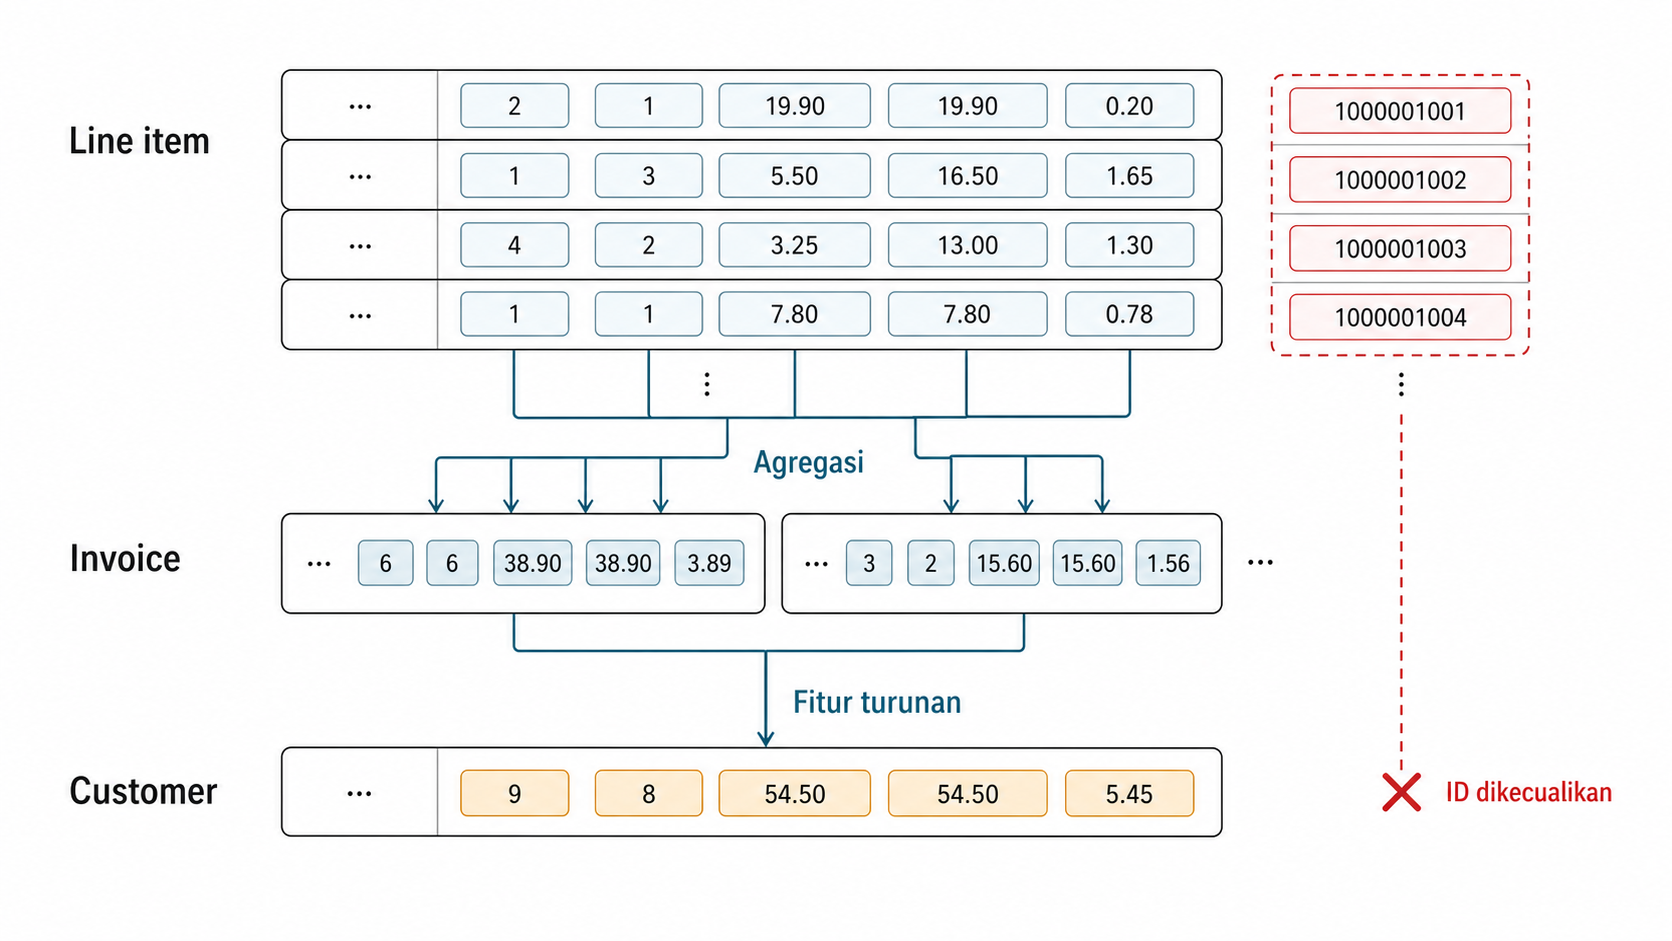
\includegraphics[width=111.6mm]{ch16-fig-1}
\caption{Deep Feature Synthesis pada entity tree}
\label{fig:ch16-fig-1}
\end{figure}

DFS membutuhkan schema, relasi antar tabel, target dataframe, time index, \emph{cutoff}, daftar primitive, dan maximum depth. Tanpa itu, mesin tidak tahu apa yang sah. Ia juga tidak punya akal domain. Jika sebuah kolom bertipe numerik, sistem dapat saja menghitung rata-rata kode pos atau maksimum nomor telepon. Angka itu valid secara komputasi, tetapi tidak bermakna sebagai fitur.

Karena itu, ruang pencarian harus diberi rem. Pertama, batasi depth agar fitur tidak meledak jumlahnya. Kedua, exclude variable yang tidak boleh diperlakukan sebagai angka, seperti ID, nomor telepon, atau kode administratif. Ketiga, tegakkan \emph{cutoff} agar hanya histori sebelum waktu prediksi yang dipakai. Aturan point-in-time dari Bab 6 tetap berlaku. Automation dengan \emph{cutoff} yang salah tidak mengurangi leakage; ia hanya menghasilkan leakage lebih cepat. DFS memperlihatkan otomasi pada level fitur relasional; langkah berikutnya memperluas pencarian ke seluruh pipeline preprocessing dan model.

\section{AutoML dan Pipeline Fitur Otomatis}\label{automl-dan-pipeline-fitur-otomatis}

Jika DFS fokus pada pembentukan fitur dari skema relasional, AutoML (Feurer et al. 2015) mencari pipeline yang lebih luas. Objek yang dicari bisa mencakup imputation, encoding, feature transformation, model selection, hyperparameter, ensembling, dan kadang feature selection. Satu kandidat pipeline dapat memakai median imputation, target encoding, dan gradient boosting. Kandidat lain dapat memakai k-NN imputation, scaling, dan SVM. Ribuan rakitan seperti ini dibandingkan melalui validasi.

Nilai AutoML adalah mengurangi pekerjaan pencarian rutin dan memberi baseline kuat (Erickson et al. 2020). Sistem AutoML yang dirancang baik dapat menjaga transformasi tetap di dalam \emph{fold} jika strategi \emph{split} dan \emph{pipeline} dikonfigurasi dengan benar. AutoML tidak otomatis menjamin pemisahan temporal atau grup yang sesuai deployment. Kemampuan menjaga batas \emph{fold} itu bagian dari nilai teknisnya, bukan hanya kenyamanan.

Namun, AutoML tetap bekerja di bawah batas yang diberikan manusia. Prediction question, unit, split strategy, metric, time budget, fairness constraint, privacy constraint, dan deployment requirement harus ditentukan lebih dulu. Jika split bocor, AutoML akan mengoptimalkan kebocoran itu dengan sangat rajin.

Gambar 16.2 menunjukkan loop pencarian AutoML. Kandidat pipeline dirakit dari menu komponen, dievaluasi dengan cross-validation, lalu skor memberi sinyal ke strategi pencarian untuk memilih kandidat berikutnya.

\begin{figure}[tbp]\centering
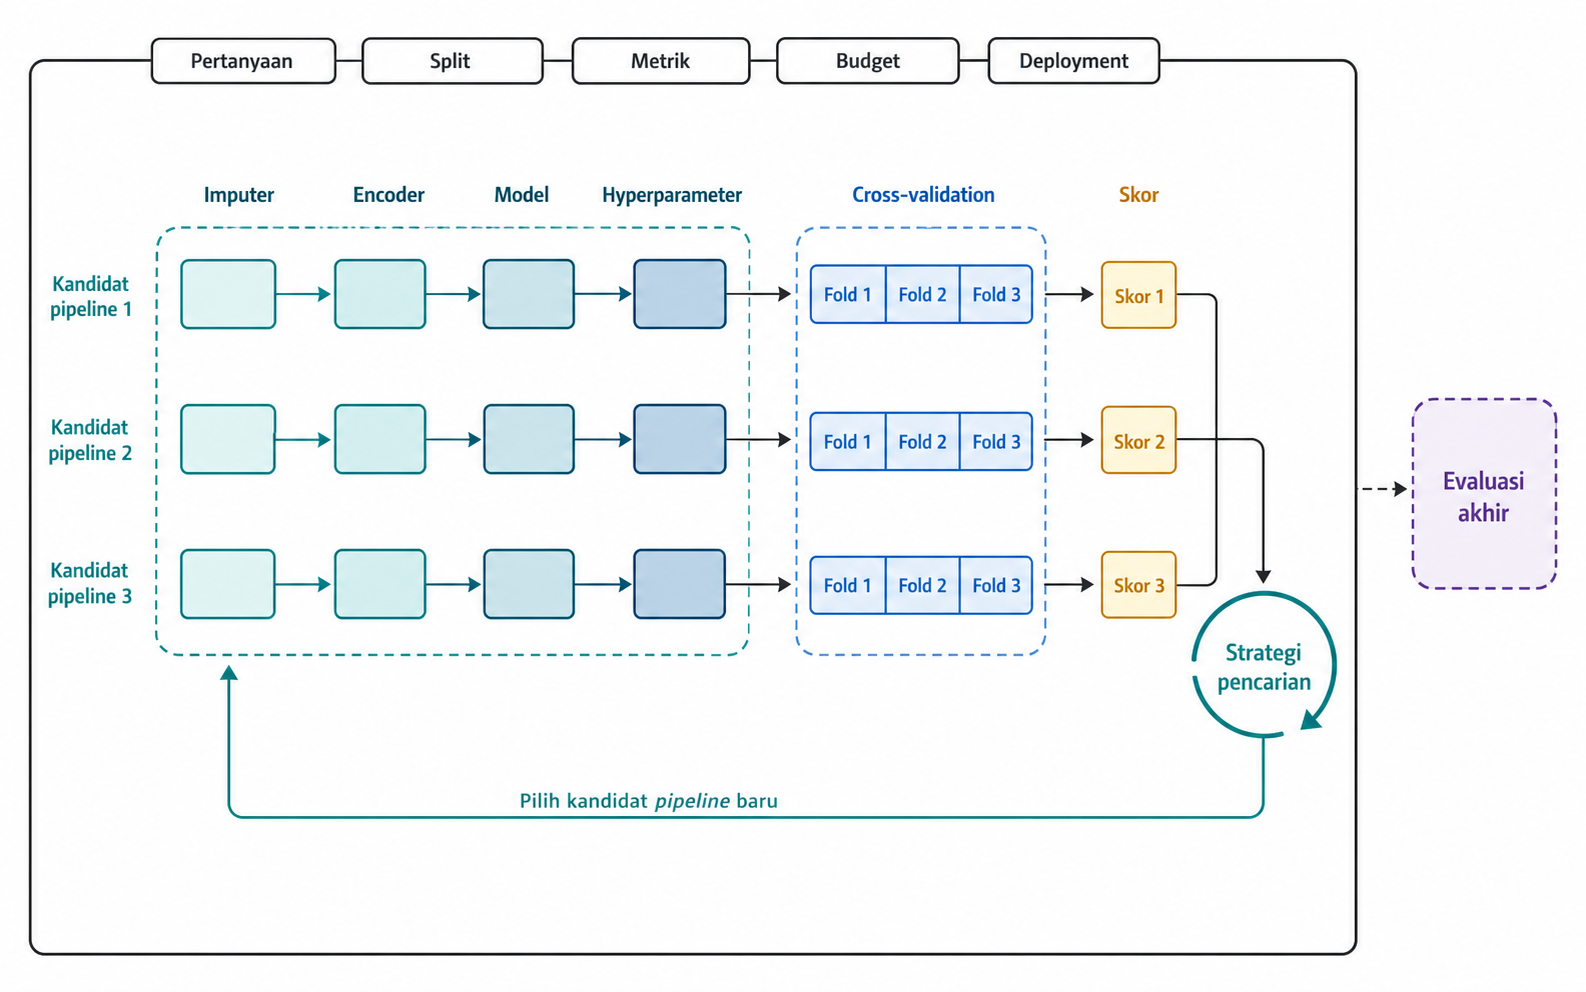
\includegraphics[width=111.6mm]{ch16-fig-2}
\caption{Loop pencarian pipeline AutoML}
\label{fig:ch16-fig-2}
\end{figure}

Risikonya ada dua. Pertama, \emph{spurious search hits}. Jika ribuan \emph{pipeline} dicoba pada \emph{fold} yang sama, sebagian dapat cocok dengan skor validasi karena kebetulan, bukan karena generalisasi. Skor inner-CV boleh memandu pencarian, tetapi tidak boleh dilaporkan sebagai estimasi performa final yang tidak bias. Gunakan \emph{nested cross-validation} atau \emph{final holdout} yang dikunci dan tidak ikut memandu pencarian untuk estimasi akhir. Ini versi industri dari peringatan Bab 2 tentang \emph{fishing}. Kedua, \emph{semantic blindness}. Sistem dapat memilih transformasi yang kuat secara statistik tetapi salah makna, misalnya memperlakukan \emph{missing sensor value} sebagai \emph{noise} padahal mesin memang sengaja dimatikan.

AutoML juga dapat membakar compute budget, menghasilkan pipeline yang sulit dijelaskan, atau memilih ensemble yang mahal dipelihara. Ketika skor sudah plateau, menambah jam pencarian sering tidak membantu. Bottleneck biasanya pindah ke kualitas data, definisi target, atau representasi. Di titik itu, manusia perlu kembali merancang fitur, bukan hanya memperpanjang search. Salah satu bentuk rancangan baru adalah meminta LLM mengusulkan fitur yang lebih semantik daripada sekadar kombinasi primitive atau pipeline.

\begin{pendalaman}{Optimasi Bayesian di balik pencarian pipeline}
Daripada mencoba semua konfigurasi atau memilih acak, banyak AutoML framework memodelkan landscape skor melalui Gaussian process surrogate dan memilih konfigurasi berikutnya dengan acquisition function. Posterior dari surrogate memberikan distribusi prediktif \(f(x)\), bukan sekadar satu nilai, sehingga ketidakpastian turut diperhitungkan. Salah satu acquisition function yang umum adalah Expected Improvement: \(EI(x) = \mathbb{E}\big[\max(f(x) - f(x^{+}),\ 0)\big]\). Di sini \(x\) adalah konfigurasi kandidat, \(f(x)\) adalah variabel acak dari posterior surrogate yang menyatakan skor yang diperkirakan beserta ketidakpastiannya, dan \(f(x^{+})\) adalah skor terbaik sejauh ini. Intuisinya, sistem menyeimbangkan eksplorasi wilayah yang belum pasti dengan eksploitasi wilayah yang tampak menjanjikan. Gagasan ini juga muncul pada hyperparameter tuning umum.
\end{pendalaman}

\section{GenAI untuk Usulan Fitur dan Risiko Fitur Semu}\label{genai-untuk-usulan-fitur-dan-risiko-fitur-semu}

Ketika DFS dan AutoML mulai dibatasi oleh primitive serta menu pipeline, GenAI atau LLM menambahkan sesuatu yang tidak dimiliki keduanya: kemampuan memakai makna bahasa. Jika metadata menyebut \passthrough{\lstinline!InvoiceDate!}, \passthrough{\lstinline!Quantity!}, \passthrough{\lstinline!UnitPrice!}, dan \passthrough{\lstinline!CustomerID!}, LLM dapat mengusulkan recency, nilai pembelian, atau frekuensi invoice. DFS mungkin hanya melihat kolom numerik dan mencoba kombinasi primitive. AutoML mungkin hanya mencoba transformasi pipeline. LLM dapat membaca nama kolom, deskripsi, dan konteks domain, lalu mengusulkan fitur semantik.

CAAFE adalah contoh pendekatan \emph{context-aware} yang memakai LLM untuk mengotomatisasi usulan rekayasa fitur pada data tabular. Salah satu pilihan implementasinya adalah memakai metadata seperti nama kolom, tipe, deskripsi, dan ringkasan konteks, bukan baris mentah. Pilihan ini dapat membatasi paparan data sensitif, tetapi bukan jaminan inheren CAAFE: metadata dan ringkasan pun dapat memuat informasi sensitif, sehingga kontrol akses, redaksi, dan kebijakan pengiriman data tetap diperlukan.

Janji utamanya adalah ideasi. LLM dapat mengusulkan rasio, recency feature, interaction, grouping, atau transformasi domain yang tidak ada dalam primitive library. Pada Online Retail, ia dapat mengusulkan jarak waktu sejak invoice terakhir, rata-rata nilai per item, proporsi return, variasi stok yang dibeli, atau fitur kalender dari bulan invoice.

Risikonya seimbang besar. LLM belajar dari co-occurrence tekstual di corpus, bukan dari sinyal statistik dalam dataset kita. Rasio yang terdengar ilmiah dapat tidak berkorelasi dengan target. Transformasi yang tampak cerdas dapat memakai tanggal setelah outcome, kategori turunan dari target, atau proxy sensitif. Kode yang dihasilkan dapat salah, mahal dihitung, atau sulit dipelihara. Jalankan kode transformasi dalam \emph{sandbox} dengan dependensi yang dibatasi, lalu uji dan tinjau sebelum menyentuh data nyata. Karena itu, usulan LLM adalah kandidat, bukan fakta.

Gambar 16.3 memperlihatkan loop proposal. Metadata masuk ke LLM, usulan fitur dieksekusi dan dievaluasi, lalu hasilnya memberi umpan balik ke putaran prompt berikutnya. Kandidat yang semu, bocor, atau tidak tersedia masuk ke reject bin.

\begin{figure}[tbp]\centering
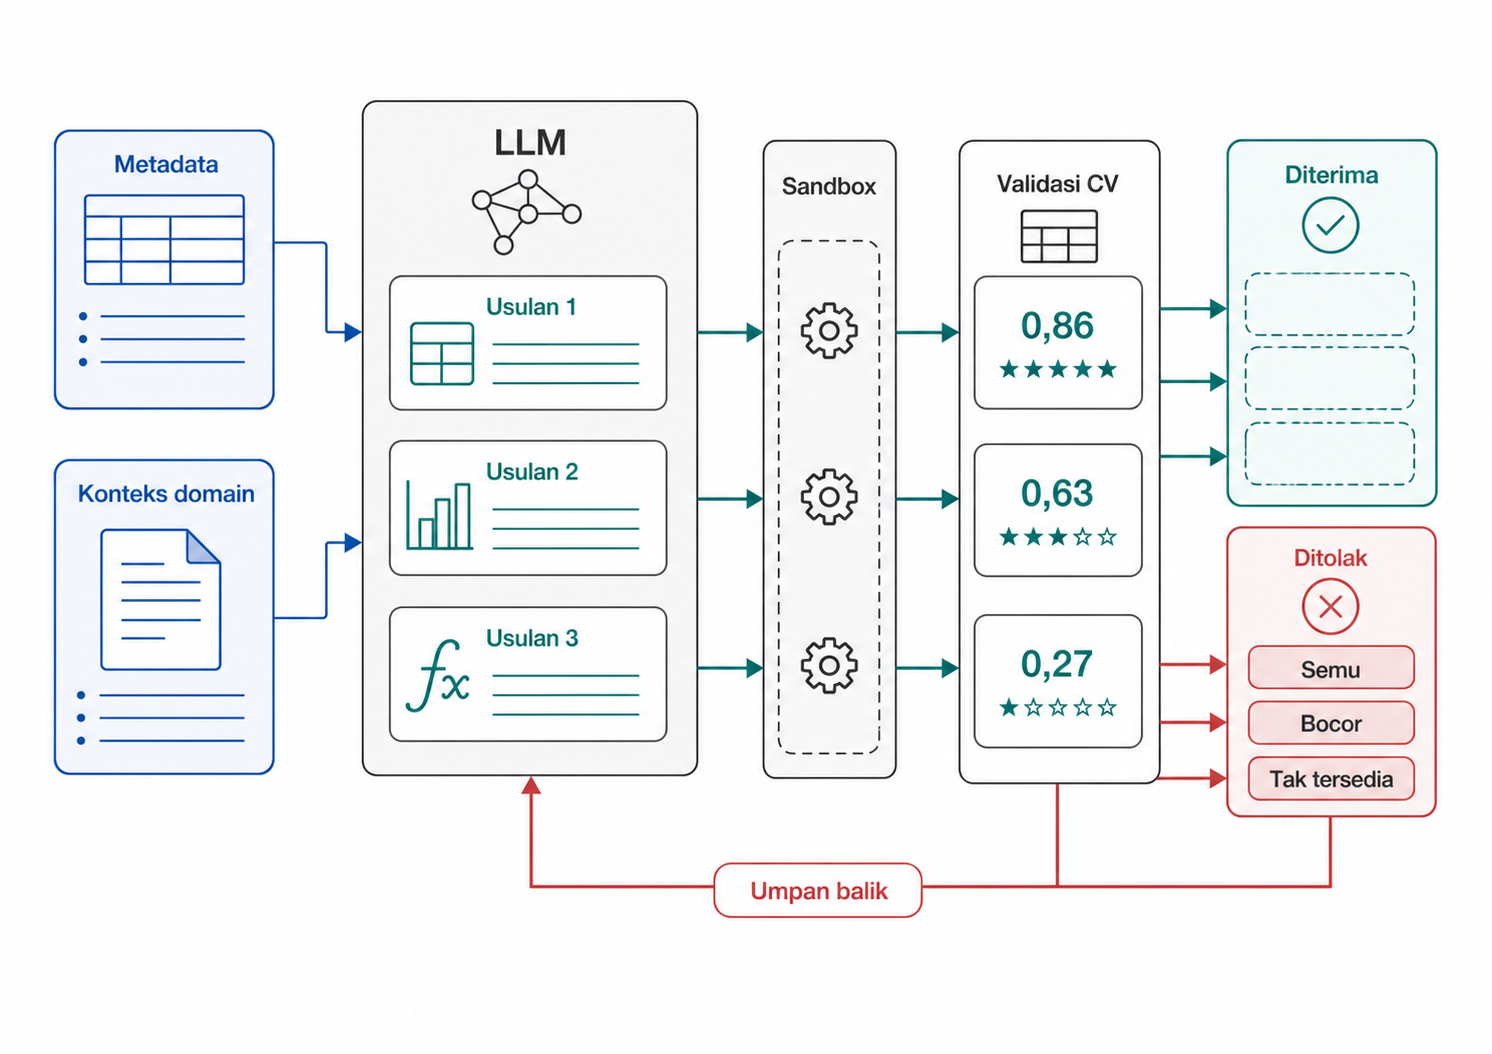
\includegraphics[width=111.6mm]{ch16-fig-3}
\caption{Loop usulan fitur berbasis LLM}
\label{fig:ch16-fig-3}
\end{figure}

Tabel 16.1 membandingkan tiga keluarga otomasi fitur. Gunakan tabel ini untuk membaca apa yang sebenarnya diotomasi dan apa yang tetap harus disediakan manusia.

\tabeljudul{Tabel 16.1 — Tiga keluarga otomasi fitur}

{\def\LTcaptype{none} % do not increment counter
\par\vspace{3pt}\noindent
\begingroup\renewcommand{\arraystretch}{1.0}%
\scriptsize\linespread{1}\selectfont
\renewcommand{\_}{\textunderscore\hspace{0pt}}%
\begin{xltabular}{\linewidth}{@{}>{\raggedright\arraybackslash}p{(\linewidth-6\tabcolsep)*\real{0.160}} >{\raggedright\arraybackslash}p{(\linewidth-6\tabcolsep)*\real{0.301}} >{\raggedright\arraybackslash}p{(\linewidth-6\tabcolsep)*\real{0.266}} >{\raggedright\arraybackslash}p{(\linewidth-6\tabcolsep)*\real{0.273}}@{}}
\toprule

Keluarga
 & 
Apa yang diotomasi
 & 
Butuh dari manusia
 & 
Risiko khas
 \\
\midrule
\endhead




DFS & Komposisi primitive atas skema relasional & Skema, primitive, \emph{cutoff}, depth & Ledakan fitur, leakage temporal \\
AutoML & Pencarian pipeline preprocessing dan model & Pertanyaan, split, metric, anggaran & Spurious hits, pipeline sulit dirawat \\
GenAI\slash{}LLM & Usulan fitur semantik dan kode & Konteks domain, gerbang validasi & Fitur semu, kode invalid, proxy sensitif \\
\bottomrule
\end{xltabular}\endgroup\par\vspace{5pt}

}

Setiap fitur usulan perlu diperiksa availability, leakage, correctness, cost, dan dampak kebijakan. Sistem baru kadang menambahkan reasoning trace pada setiap transformasi agar manusia dapat membaca rationale, bukan hanya skor. Tetapi rationale pun harus diaudit; kalimat yang masuk akal belum tentu fitur yang sah. Karena itu, putaran proposal harus berakhir pada workflow human-in-the-loop, bukan pada penerimaan otomatis.

\begin{pendalaman}{LLM sebagai pengoptimal evolusioner}
Arah riset terbaru memperlakukan rekayasa fitur sebagai \emph{program search}. LLM mengusulkan \emph{script} transformasi, evaluator menjalankannya, lalu nilai marginalnya diukur dengan delta-CV: \(\text{Fitness}(f) = \text{CV}(\mathcal{M},\ X \cup \{f\},\ Y) - \text{CV}(\mathcal{M},\ X,\ Y)\), dengan \(\mathcal{M}\) sebagai model baseline, \(X\) sebagai kumpulan fitur saat ini, \(Y\) sebagai target, dan \(\text{CV}(\cdot)\) sebagai skor validasi silang. Skor itu kembali ke konteks LLM, sehingga putaran berikutnya dapat memutasi dan menggabungkan program yang lebih baik. Polanya mirip \emph{genetic algorithm} dengan LLM sebagai \emph{mutation operator}. Namun, \emph{quality control} utama tetap pada \emph{fitness gate}; LLM hanya memperlebar \emph{funnel} kandidat.
\end{pendalaman}

\section{Human-in-the-Loop: Validasi dan Kurasi Fitur Usulan Mesin}\label{human-in-the-loop-validasi-dan-kurasi-fitur-usulan-mesin}

Setelah tiga keluarga otomasi terlihat, bagian pentingnya adalah gerbang penerimaan. Rekayasa fitur \emph{human-in-the-loop} (Amershi et al. 2014) berarti manusia tidak hanya hadir di akhir untuk membaca \emph{leaderboard}. Manusia mendefinisikan ruang kerja sejak awal: unit, target, \emph{cutoff}, \emph{split}, metrik, operator yang diizinkan, batas \emph{latency}, dan fitur yang dilarang. Mesin kemudian mengeksplorasi kandidat dalam koridor itu. Manusia kembali sebagai kurator, membaca skor sekaligus alasan, risiko, dan kelayakan operasional.

Workflow yang baik dimulai dari definisi task. Setelah itu, kandidat fitur dibuat secara otomatis oleh DFS, AutoML, LLM, atau kombinasi. Kandidat pertama disaring secara keras: bocor, tidak tersedia, mahal dihitung, melanggar kebijakan, atau tidak masuk akal secara semantik. Kandidat yang lolos diuji dengan ablation, stability check, dan validasi yang sesuai split. Fitur yang diterima dan ditolak sama-sama didokumentasikan, karena keputusan penolakan sering sama pentingnya dengan keputusan penerimaan.

Tabel 16.2 merangkum pembagian peran manusia dan mesin. Baris-barisnya menunjukkan bahwa mesin paling kuat pada eksplorasi dan ranking, sedangkan manusia memegang definisi, batas, kurasi, dan tanggung jawab. Gunakan tabel ini sebagai audit sederhana: jika sebuah tahap penting tidak punya pemilik manusia, workflow otomasi belum aman.

\tabeljudul{Tabel 16.2 — Pembagian peran manusia-mesin}

{\def\LTcaptype{none} % do not increment counter
\par\vspace{3pt}\noindent
\begingroup\renewcommand{\arraystretch}{1.0}%
\scriptsize\linespread{1}\selectfont
\renewcommand{\_}{\textunderscore\hspace{0pt}}%
\begin{xltabular}{\linewidth}{@{}>{\raggedright\arraybackslash}p{(\linewidth-4\tabcolsep)*\real{0.195}} >{\raggedright\arraybackslash}p{(\linewidth-4\tabcolsep)*\real{0.495}} >{\raggedright\arraybackslash}p{(\linewidth-4\tabcolsep)*\real{0.310}}@{}}
\toprule

Tahap
 & 
Manusia
 & 
Mesin
 \\
\midrule
\endhead




Definisi masalah & Menentukan unit, target, \emph{cutoff}, metric & - \\
Ruang pencarian & Menetapkan batasan, primitive, DSL & Mengeksekusi aturan yang diizinkan \\
Eksplorasi dan pengujian & Menyediakan split dan kriteria & Membuat kandidat, CV, ranking \\
Kurasi & Menilai kelayakan semantik, kepatuhan, latency & Menyajikan skor dan trace \\
Dokumentasi dan monitoring & Mengelola siklus hidup fitur: keputusan penerimaan, pemilik, pemantauan drift & Menghasilkan log, laporan, alert; mendeteksi anomali \\
\bottomrule
\end{xltabular}\endgroup\par\vspace{5pt}

}

Gambar 16.4 menggambarkan gerbang kerja tersebut. Perhatikan dua gate: statistical validation dan human curation. Fitur yang lulus skor tetapi gagal kebijakan tetap ditolak.

\begin{figure}[tbp]\centering
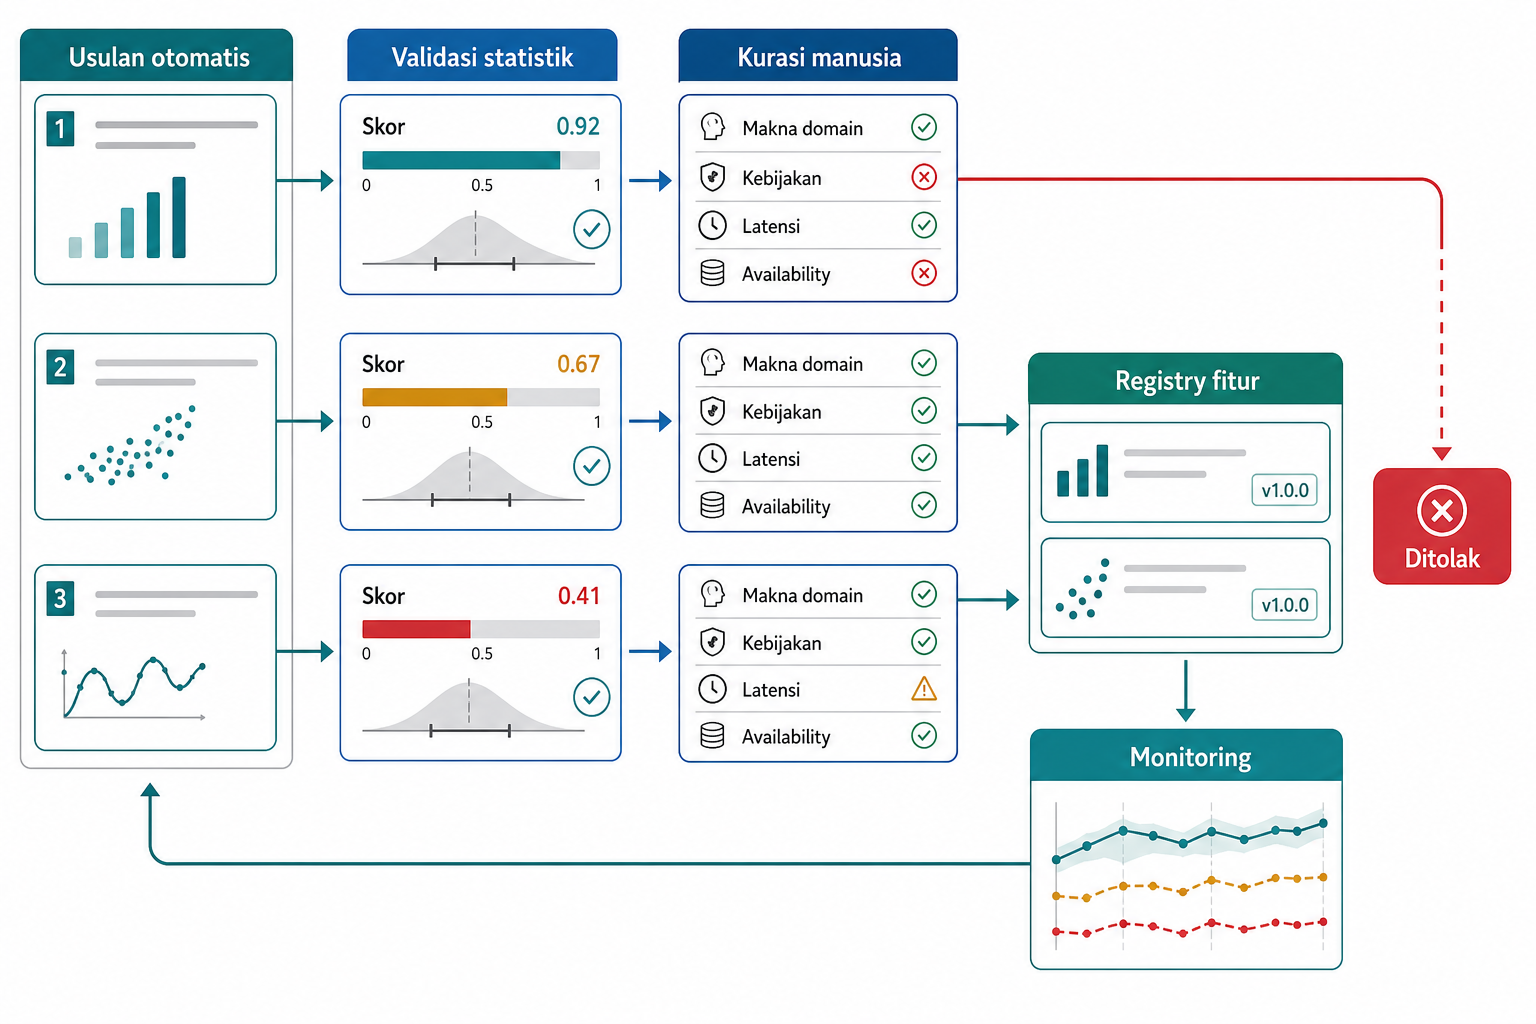
\includegraphics[width=111.6mm]{ch16-fig-4}
\caption{Workflow human-in-the-loop untuk fitur otomatis}
\label{fig:ch16-fig-4}
\end{figure}

Apa yang hanya dapat ditangkap kurator? Pertama, fitur yang sangat kuat tetapi tidak punya dasar rasional, sehingga kemungkinan spurious. Kedua, fitur yang lolos pemeriksaan row-level tetapi mustahil dihitung dalam latency produksi. Ketiga, fitur yang secara statistik membantu tetapi merekonstruksi protected attribute melalui proxy, seperti pelajaran Bab 9.

Pada audit Online Retail, automated synthesis menghasilkan banyak kandidat. Beberapa tampak sangat dominan karena sebenarnya membaca masa depan, misalnya hitungan invoice positif dalam 60 hari setelah \emph{cutoff} atau nilai belanja masa depan. Kandidat lain seperti \passthrough{\lstinline!CustomerID!} bisa dihitung, tetapi tidak bermakna sebagai angka yang boleh dirata-ratakan atau dibandingkan jaraknya. Fitness function melihat skor tinggi; manusia melihat temporal leak atau semantic misuse. Perbaikannya bukan sekadar membuang satu fitur, tetapi menutup keluarga fitur serupa dan memperketat konfigurasi \emph{cutoff}.

Inilah batas dan kekuatan kolaborasi manusia-AI. Automation tetap berada di wilayah representasi yang dirancang manusia ketika manusia menentukan primitive, constraint, DSL, dan acceptance rule. Mesin memperluas pencarian; manusia menjaga makna, ketersediaan, kebijakan, dan deployment. Bab 17 menutup buku dengan prinsip yang lebih umum: alat boleh berubah, tetapi pipeline dan evaluasi harus tetap dirancang dengan disiplin.

\begin{sintesis}

Benang merah Bab 16 adalah bahwa rekayasa fitur otomatis memperbesar ruang kandidat, bukan menghapus tanggung jawab desain. DFS menyusun primitive pada skema relasional, AutoML mencari pipeline di bawah metric dan split yang diberikan, sedangkan GenAI mengusulkan fitur semantik dari metadata dan konteks. Tabel 16.1 membantu membedakan apa yang diotomasi oleh masing-masing keluarga.

Risiko utamanya juga berbeda: ledakan fitur dan leakage temporal pada DFS, spurious search hits dan pipeline sulit dirawat pada AutoML, serta fitur semu, kode invalid, dan proxy sensitif pada LLM. Tabel 16.2 merangkum pembagian kerja yang sehat: manusia mendesain koridor dan mengurasi, mesin mengeksplorasi dan meranking. Dua tabel itu perlu dibaca bersama: keluarga otomasi menentukan kandidat yang muncul, sedangkan pembagian peran menentukan siapa yang boleh menerimanya.

Pesan bab ini sederhana. Otomasi yang baik bukan ``sekali klik lalu selesai'', melainkan kolaborasi yang diberi batas. Semakin kuat mesin menghasilkan kandidat, semakin penting manusia mendefinisikan masalah, split, \emph{cutoff}, metric, dan acceptance rule.

\end{sintesis}

\begin{bacaan}

\begin{itemize}
\tightlist
\item
  Featuretools (Kanter \& Veeramachaneni 2015, DSAA) --- \url{https://featuretools.alteryx.com/}. Deep Feature Synthesis otomatis.
\item
  auto-sklearn (Feurer dkk. 2015) --- \url{https://automl.github.io/auto-sklearn/}. AutoML termasuk praproses fitur.
\item
  CAAFE (Hollmann dkk. 2023) --- \url{https://arxiv.org/abs/2305.03403}. Rekayasa fitur berbantuan LLM yang context-aware.
\item
  LLM-FE (Abhyankar dkk. 2025) --- \url{https://arxiv.org/abs/2503.14434}. Fitur yang diusulkan LLM dengan evaluasi terukur.
\item
  scikit-learn --- Common Pitfalls --- \url{https://scikit-learn.org/stable/common_pitfalls.html}. Menjaga fitting per-fold pada pipeline otomatis.
\item
  Shahriari dkk. (2016), Bayesian Optimization (Proc. IEEE) --- \url{https://doi.org/10.1109/JPROC.2015.2494218}. Dasar optimisasi hiperparameter.
\end{itemize}

\end{bacaan}

\rujukanheading

\protect\phantomsection\label{refs}
\begin{CSLReferences}{1}{1}
\bibitem[\citeproctext]{ref-amershi2014power}
Amershi, Saleema, Maya Cakmak, W. Bradley Knox, and Todd Kulesza. 2014. {``Power to the People: The Role of Humans in Interactive Machine Learning.''} \emph{AI Magazine} 35 (4): 105--20.

\bibitem[\citeproctext]{ref-erickson2020autogluon}
Erickson, Nick, Jonas Mueller, Alexander Shirkov, et al. 2020. \emph{{AutoGluon-Tabular}: Robust and Accurate {AutoML} for Structured Data}. \url{https://arxiv.org/abs/2003.06505}.

\bibitem[\citeproctext]{ref-feurer2015autosklearn}
Feurer, Matthias, Aaron Klein, Katharina Eggensperger, Jost Springenberg, Manuel Blum, and Frank Hutter. 2015. {``Efficient and Robust Automated Machine Learning.''} \emph{Advances in Neural Information Processing Systems (NeurIPS)}.

\bibitem[\citeproctext]{ref-kanter2015dfs}
Kanter, James Max, and Kalyan Veeramachaneni. 2015. {``Deep Feature Synthesis: Towards Automating Data Science Endeavors.''} \emph{IEEE International Conference on Data Science and Advanced Analytics (DSAA)}. \url{https://doi.org/10.1109/DSAA.2015.7344858}.

\end{CSLReferences}

% ==========================================================================
% ch17.tex — dihasilkan dari v2/drafts oleh tools/md2tex.py
% Sumber: v2\drafts\ch17\ch17_draft_v2.md
% Boleh disunting manual; menjalankan md2tex.py lagi akan menimpa.
% ==========================================================================
\chapter{Sintesis: Merancang Pipeline dan Prinsip yang Bertahan Lama}\label{sintesis-merancang-pipeline-dan-prinsip-yang-bertahan-lama}

Rekayasa fitur sering tampak seperti kumpulan teknik yang terpisah, mulai dari penskalaan, pengodean, lag, embedding, centrality graf, hingga AutoML. Setelah enam belas bab, gambaran yang lebih penting seharusnya terlihat. Fitur adalah keputusan representasi yang hidup di dalam pipeline. Keputusan itu harus cocok dengan tujuan prediksi, tersedia pada waktu prediksi, mengikuti pemisahan data, dapat dipelihara, dan terbukti membantu melalui validasi.

Bab penutup ini mengubah isi buku menjadi kerangka kerja, dimulai dari pertanyaan paling awal, yaitu apa yang akan diprediksi dan kapan informasi tersedia, menuju pertanyaan operasional tentang konsistensi pelatihan-inferensi, validasi skema, versioning, dan pemantauan perubahan data (drift). Peta keputusan representasi, kebocoran, dan validasi lintas tipe data disajikan sebagai rujukan cepat. Bab ini menguraikan dua prinsip penutup, yaitu mulai dari masalah, ketersediaan, dan pemisahan data sebelum membuat fitur, serta validasi mengalahkan jumlah fitur.

\section{\texorpdfstring{Kerangka Desain: dari Tujuan Prediksi ke \emph{Pipeline} Final}{Kerangka Desain: dari Tujuan Prediksi ke Pipeline Final}}\label{kerangka-desain-dari-tujuan-prediksi-ke-pipeline-final}

Proyek rekayasa fitur yang baik tidak dimulai dari teknik favorit. Ia dimulai dari tujuan prediksi. Apa keputusan yang akan dibantu model? Apa konsekuensi salah prediksi? Kapan prediksi dibuat? Data apa yang benar-benar tersedia pada waktu itu?

Empat definisi menjadi tulang punggung masalah sebelum satu baris transformasi dibuat: unit analisis, target, horizon, dan \emph{cutoff}. Unit menjawab satu baris mewakili apa: pelanggan per bulan, transaksi, sesi pemeriksaan, produk per minggu, atau node dalam graf. Target menjawab apa yang diprediksi. Horizon menjawab seberapa jauh ke depan. \emph{Cutoff} menjawab batas informasi yang sah sebelum prediksi.

Kesalahan di tahap ini tidak dapat diperbaiki oleh fitur yang canggih. Jika target salah dirumuskan, model mengoptimalkan masalah yang salah. Jika \emph{cutoff} kabur, leakage masuk lewat pintu belakang. Jika unit terlalu kasar atau terlalu halus, fitur menjadi tidak stabil.

Setelah itu, pilih \emph{split} yang meniru deployment. \emph{Random split} cocok ketika baris dapat dipertukarkan di bawah protokol penggunaan. Entitas berulang bukan otomatis \emph{leakage}: untuk memprediksi masa depan pelanggan yang sudah dikenal, gunakan evaluasi temporal dan fitur \emph{point-in-time}; gunakan \emph{group split} jika deployment menuntut generalisasi ke pelanggan baru. Demikian pula, kedekatan lokasi atau \emph{edge} lintas \emph{train-test} tidak otomatis bocor. Gunakan \emph{spatial block}, buffer, evaluasi \emph{transductive}, \emph{inductive split}, atau \emph{temporal graph split} sesuai lokasi, hubungan, dan informasi yang benar-benar tersedia saat inferensi. Pada masalah nyata, \emph{split} bisa \emph{hybrid}.

Baru setelah itu kita memilih sumber fitur dan struktur representasi: tabular, sequence, teks, citra, audio, spasial, graf, atau multimodal. Dari struktur itu muncul transformasi yang sesuai: \emph{scaling}, \emph{encoding}, \emph{derived features}, \emph{selection}, \emph{dimensionality reduction}, \emph{embeddings}, \emph{pretrained encoders}, atau \emph{automated feature proposals}. \emph{Baseline} harus hadir sebelum kompleksitas bertambah.

Gambar 17.1 merangkum seluruh kerangka buku sebagai satu band desain. Diagram ini dapat dibaca sebagai checklist awal setiap proyek.

\begin{figure}[tbp]\centering
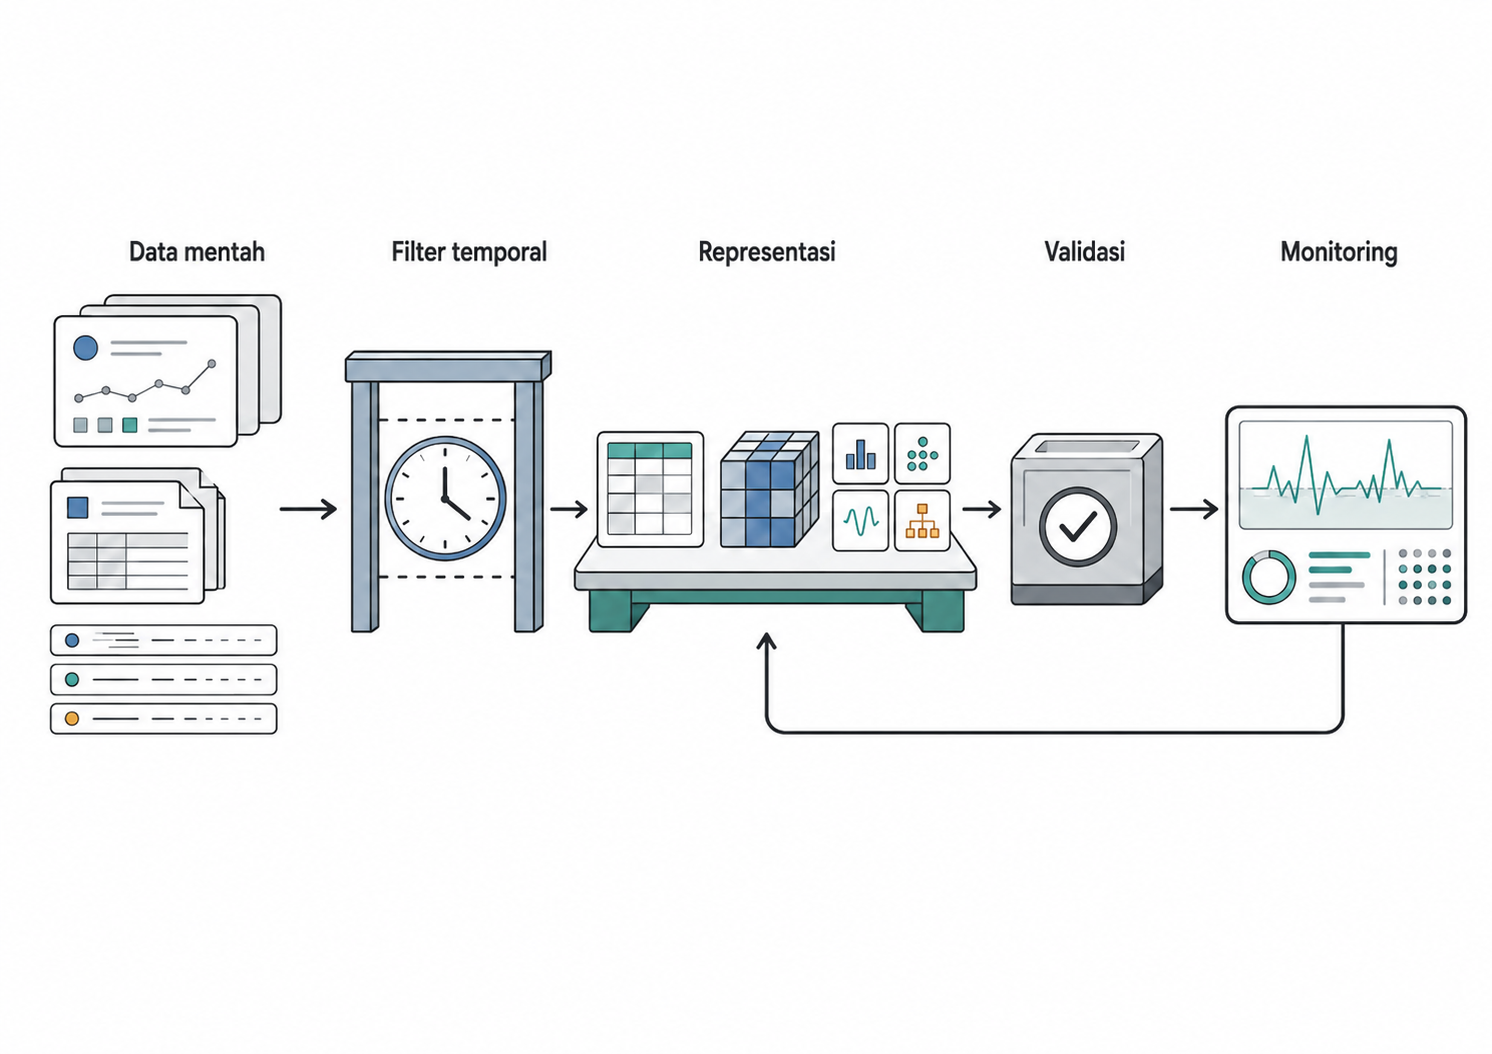
\includegraphics[width=111.6mm]{ch17-fig-1}
\caption{Kerangka desain rekayasa fitur dari awal sampai produksi}
\label{fig:ch17-fig-1}
\end{figure}

Contoh mikro: sistem credit approval. Tujuannya memperkirakan default risk. Unitnya satu loan application. Targetnya default dalam 12 bulan. \emph{Split}-nya temporal berdasarkan tanggal aplikasi. Hanya setelah ini agregat histori pembayaran, rasio pendapatan, dan fitur perilaku diuji terhadap \emph{baseline} logistic regression. Urutan ini tampak sederhana, tetapi ia mencegah banyak kesalahan yang tidak terlihat jika proyek dimulai dari teknik.

\emph{Pipeline} final harus mereproduksi transformasi pelatihan pada \emph{inference}. Ia menyimpan \emph{fitted state}, urutan transformasi, daftar fitur, versi encoder, dan keputusan \emph{cutoff}. Dokumentasi bukan pekerjaan administratif belakangan; ia adalah cara agar representasi dapat dipercaya ulang. Kerangka desain ini baru kuat jika definisi yang sama bertahan saat model masuk ke \emph{inference}.

\section{Konsistensi Training-Inference dan Training-Serving Skew}\label{konsistensi-training-inference-dan-training-serving-skew}

Kerangka desain baru sah jika definisi yang dibuat saat pelatihan bertahan saat model melayani prediksi (Sculley et al. 2015). \emph{Training-inference consistency} berarti definisi fitur dan logika transformasi sama saat pelatihan, validasi, dan \emph{serving}. Ini kontrak Bab 2, tetapi pada skala sistem. Jika pelatihan memakai satu cara menghitung fitur dan produksi memakai cara lain, model tidak lagi melihat distribusi yang sama.

\emph{Training-serving skew} sering muncul diam-diam. \emph{Reimplementation drift} terjadi ketika logika eksperimen di Python ditulis ulang di backend lain dengan aturan rounding, null handling, atau timezone yang berbeda. \emph{Live recomputation} terjadi ketika produksi menghitung ulang statistik dari \emph{streaming} data, padahal pelatihan memakai statistik beku dari \emph{training split}. Tidak selalu ada error log. Prediksi hanya menurun diam-diam.

\emph{Fitted transformation} harus menyimpan state: rata-rata dan standard deviation scaler, nilai imputasi, kategori encoder, \emph{vocabulary}, \emph{selected features}, version model, version tokenizer, dan version \emph{embedding}. \emph{Feature availability} juga tidak bisa ditawar. Jika fitur hanya ada setelah keputusan dibuat, fitur itu invalid meskipun sangat prediktif.

Gambar 17.2 memperlihatkan pola \emph{feature store}. Definisi fitur berada di pusat, lalu mengalir ke \emph{offline store} untuk pelatihan historis dan \emph{online store} untuk \emph{serving} rendah latency.

\begin{figure}[tbp]\centering
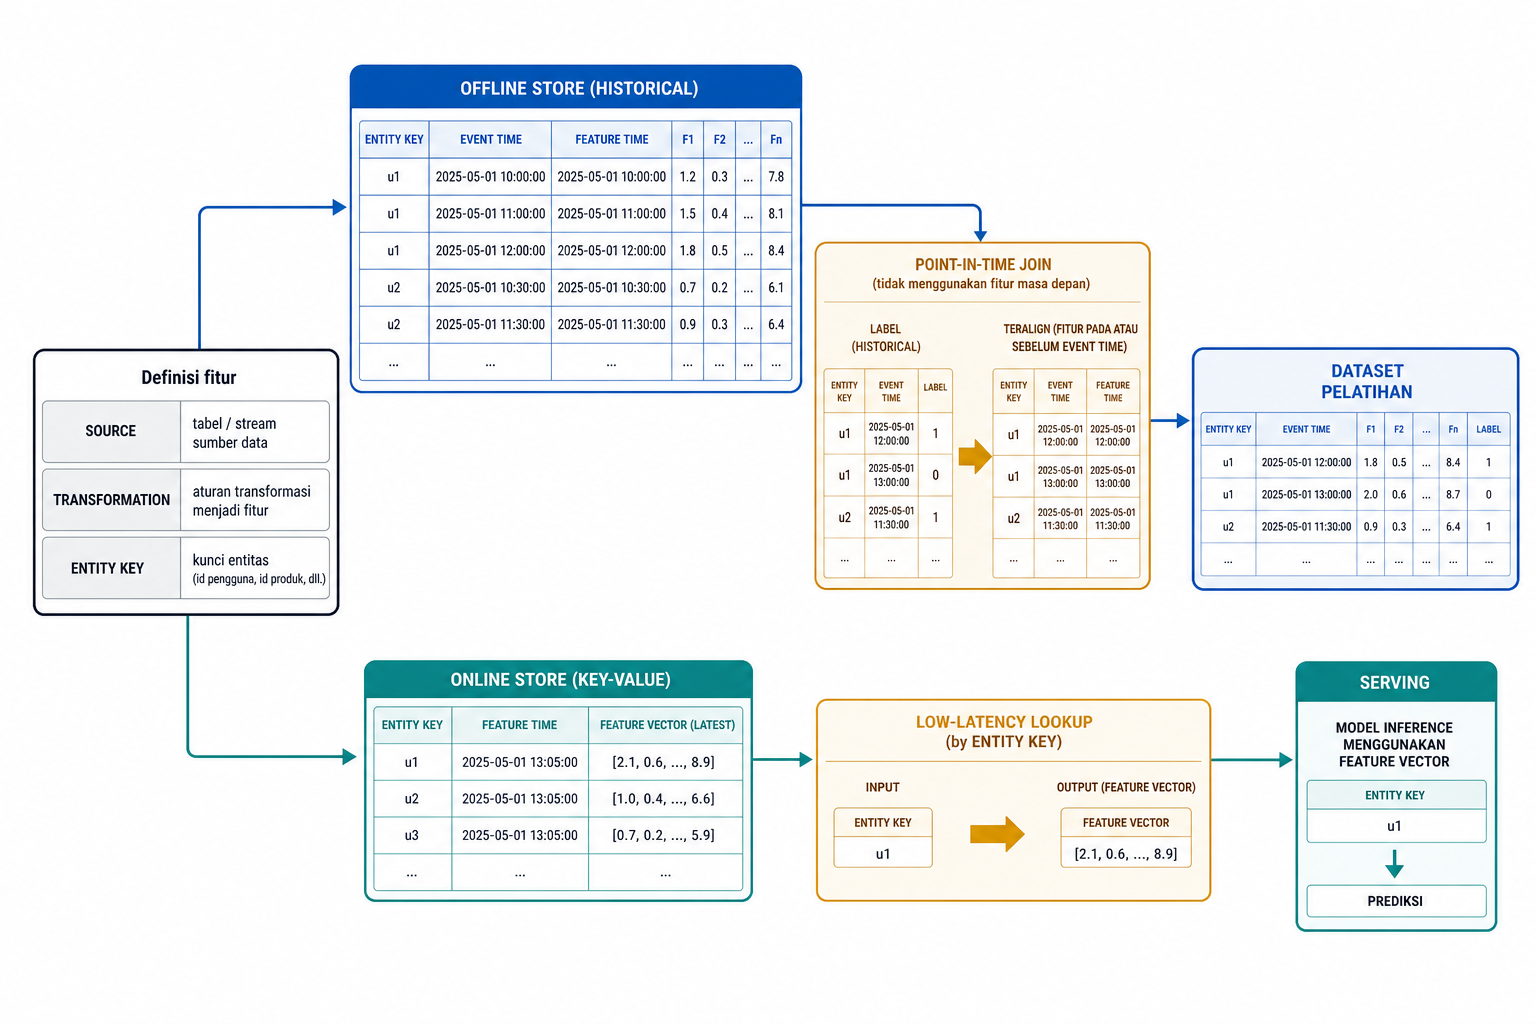
\includegraphics[width=111.6mm]{ch17-fig-2}
\caption{\emph{Feature store}: definisi fitur untuk pelatihan dan \emph{serving}}
\label{fig:ch17-fig-2}
\end{figure}

Pada skala kecil, \emph{pipeline} yang diserialisasi dengan baik sudah mewakili gagasan yang sama: satu definisi, satu urutan transformasi, satu state yang dipakai ulang. Pada skala besar, definisi fitur dipusatkan agar tim pelatihan dan tim backend tidak menghitung fitur dengan logika berbeda.

Contohnya sederhana. Pelatihan memakai CSV yang sudah dibersihkan, tetapi produksi membaca database live dengan kode \emph{missing value} yang berbeda. \emph{Text vectorizer} di-\emph{fit} pada korpus pelatihan, lalu \emph{vocabulary} dan IDF yang sama harus dipakai ulang di produksi. Istilah ``korpus lengkap'' dalam konteks ini hanya boleh berarti seluruh korpus pelatihan yang sah, bukan validasi atau \emph{test}. Kedua kasus ini bukan masalah model; ini masalah representasi yang tidak konsisten. Konsistensi juga perlu dijaga setelah sistem berjalan, melalui \emph{schema validation}, \emph{versioning}, dan \emph{drift monitoring}.

\begin{pendalaman}{\emph{Feature store}: satu definisi, dua mesin}
\emph{Feature store} memusatkan definisi fitur dan membagi penyimpanan menjadi \emph{offline store} untuk histori skala warehouse dan \emph{online store} untuk \emph{inference} rendah latency. Dua jaminan utamanya adalah \emph{point-in-time-correct historical joins}, yaitu aturan \emph{cutoff} Bab 1 dan Bab 6 yang dilembagakan, serta satu \emph{serving interface} agar tim backend tidak mengimplementasikan ulang logika fitur. Untuk proyek kelas atau riset kecil, \emph{pipeline} yang disimpan rapi adalah versi sederhana dari prinsip yang sama: definisi fitur tidak boleh bercabang diam-diam.
\end{pendalaman}

\section{Schema Validation, Versioning, dan Drift}\label{schema-validation-versioning-dan-drift}

Konsistensi tidak cukup dijaga sekali saat model dikirim. \emph{Pipeline} yang baik perlu gerbang produksi (Breck et al. 2017). \emph{Schema validation} memeriksa apakah data masuk memiliki kolom, tipe, rentang, kategori, pola \emph{missingness}, dan hubungan yang diharapkan. Tooling seperti TFDV, Great Expectations, atau pemeriksaan runtime bergaya Pandera berada dalam keluarga ini. Jika input melanggar kontrak, sistem sebaiknya memberi alert atau menolak \emph{batch}, bukan diam-diam mengubah data menjadi bentuk yang salah.

\emph{Transformation versioning} mencatat logika fitur, \emph{fitted parameters}, model atau encoder version, dan data contract yang menghasilkan feature set. Nilai operasionalnya adalah rollback. Jika prediksi produksi tiba-tiba menyimpang, tim dapat kembali ke versi \emph{pipeline} fitur terakhir yang stabil sambil menyelidiki penyebab. Tooling bergaya DVC mengikat code, data, dan model checkpoint agar perubahan dapat ditelusuri.

\emph{Data drift} atau \emph{covariate drift} berarti \(P(X)\) berubah, sedangkan \emph{concept drift} (Gama et al. 2014) berarti \(P(Y\mid X)\) berubah. \emph{Population shift} menamai perubahan komposisi populasi; dampaknya dapat terlihat sebagai perubahan \(P(X)\) atau prevalensi label \(P(Y)\) dan tidak otomatis berarti \emph{concept drift}. Jika sensor baru mengganti rentang nilai, itu mungkin \emph{data drift} mekanis. Jika komposisi pelanggan berubah setelah kebijakan baru, itu dapat menjadi \emph{population shift}. Jika hubungan perilaku dengan target atau definisi target berubah, pemeriksaannya lebih mendasar.

Bab 9 sudah membahas PSI; di sini cukup diingat bahwa nilai besar, misalnya konvensi investigasi di atas 0,25, memicu pemeriksaan, bukan keputusan otomatis. Untuk \emph{drift} multivariat pada fitur kontinu, ukuran jarak seperti \emph{Wasserstein distance} dapat dipakai. Monitoring harus memprioritaskan fitur penting dan rapuh, bukan semua statistik dengan bobot sama.

Gambar 17.3 merangkum tiga \emph{guardrail}. \emph{Schema gate} menolak input cacat, \emph{versioned transformation layer} menjaga rollback, dan \emph{drift monitor} memberi alert yang harus diselidiki.

\begin{figure}[tbp]\centering
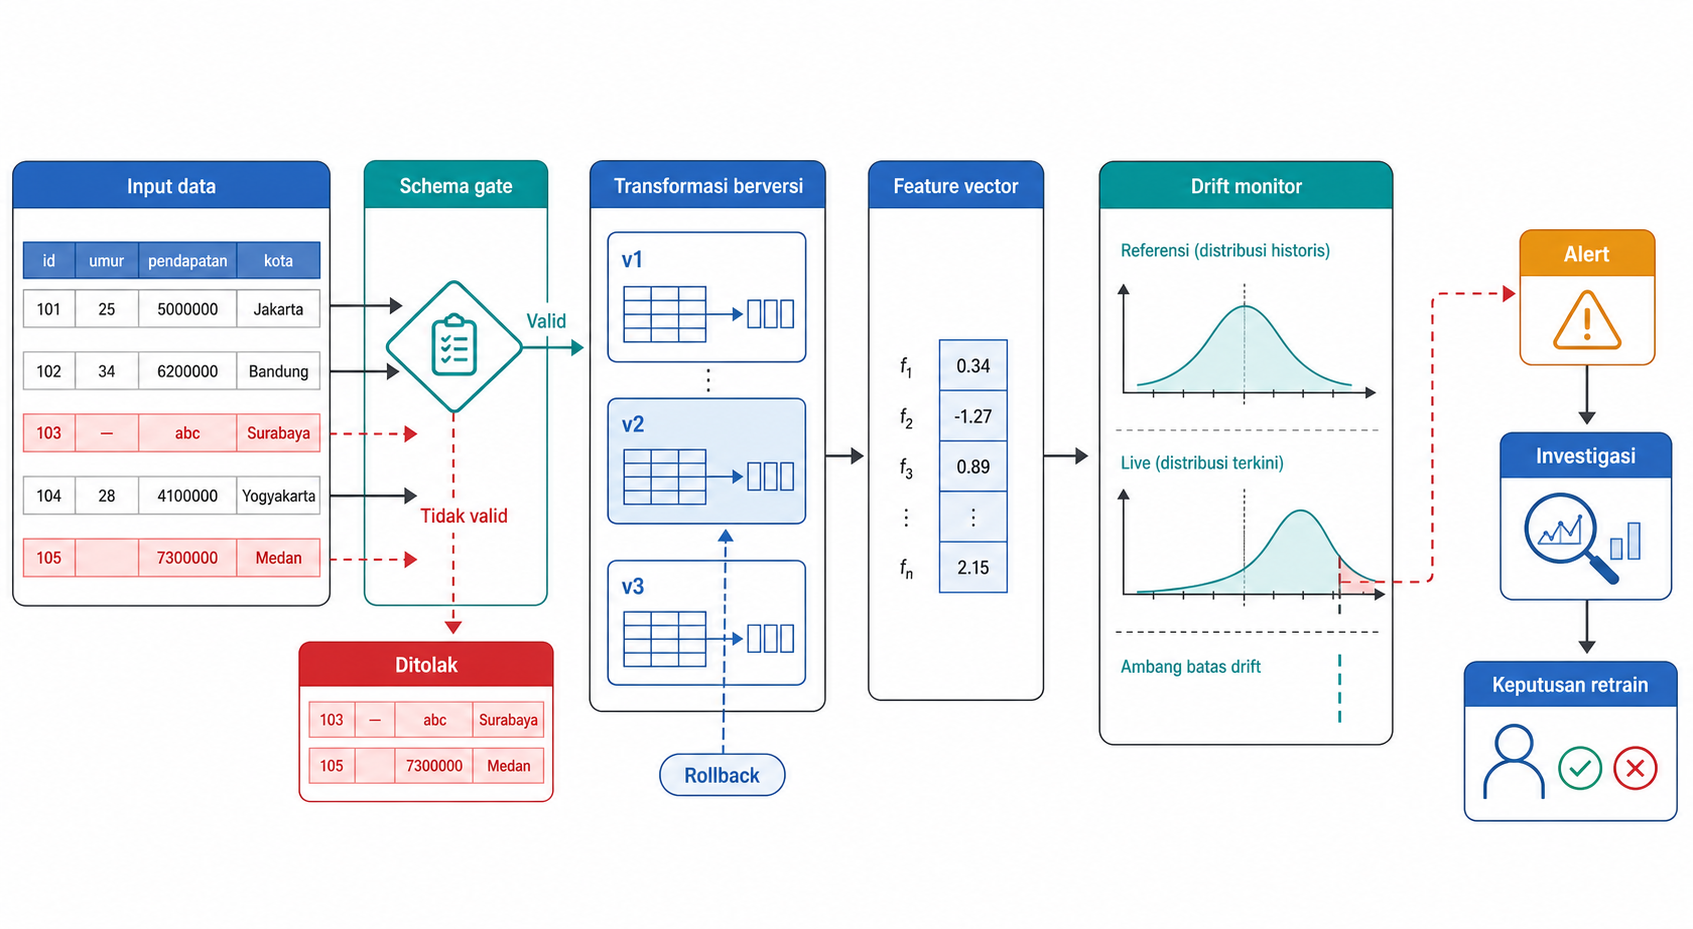
\includegraphics[width=111.6mm]{ch17-fig-3}
\caption{Guardrail produksi untuk fitur}
\label{fig:ch17-fig-3}
\end{figure}

Respons terhadap \emph{drift} harus bertahap. Pertama, bedakan sebab mekanis dari perubahan populasi organik: sensor rusak, sync gagal, kategori baru, atau format input berubah. Teks masukan pengguna juga dapat berubah setelah kebijakan baru atau migrasi platform, misalnya formulir \emph{online} yang diganti formatnya. Kedua, jika perubahan organik terbukti melewati toleransi dan memengaruhi performa, jadwalkan retraining dengan data terbaru. Jangan mematikan model otomatis hanya karena satu alert \emph{drift} menyala. Dengan \emph{guardrail} ini, kita dapat kembali ke pertanyaan desain: representasi apa yang wajar untuk tipe data dan batas operasional tertentu?

\begin{pendalaman}{Memantau performa tanpa label: estimasi berbasis keyakinan}
Masalah monitoring paling sulit adalah label produksi sering terlambat minggu atau bulan. Estimator modern mencoba memprediksi dampak performa dari \emph{drift} yang terlihat, memakai distribusi input dan \emph{confidence} model sebelum label tiba. \emph{Confidence-based performance estimation} dan \emph{direct loss estimation}, misalnya, memperkirakan apakah AUC atau loss sedang memburuk. Ini estimasi dengan asumsi, bukan pengukuran; salah satu asumsi pentingnya adalah \emph{concept drift} tidak dominan. Nilainya adalah peringatan dini. Evaluasi berbasis label tetap menjadi penyelesaian akhir ketika ground truth tiba.
\end{pendalaman}

\section{Peta Rute Lintas Tipe Data}\label{peta-rute-lintas-tipe-data}

Sebelum memilih modalitas, cabang pertama sering bersifat operasional: \emph{batch} atau \emph{streaming}. Agregat histori satu bulan mungkin wajar untuk scoring malam hari, tetapi mustahil untuk \emph{serving} milidetik jika data harus dihitung ulang live. \emph{Latency}, \emph{freshness}, dan biaya sering memangkas menu fitur sebelum teknik dipilih.

Peta rute pada bagian ini melengkapi peta operasi yang sudah dibangun sejak awal buku. Bab 3-9 membantu menjawab apa yang dilakukan terhadap fitur: \emph{scaling}, \emph{encoding}, imputasi, agregasi, seleksi, reduksi, dan evaluasi. Bagian ini membantu menjawab bentuk data apa yang sedang dihadapi: tabular, deret waktu, teks, citra, audio, spasial, graf, atau multimodal. Dalam proyek nyata, dua peta ini dipakai bersama.

Setelah itu, cocokkan representasi dengan tipe data, model, ukuran data, interpretabilitas, compute, dan deployment constraint. Tabel 17.1 adalah router lintas bab. Ia tidak memilihkan model secara otomatis, tetapi membantu pembaca bertanya: representasi awal apa yang wajar, \emph{leakage} apa yang paling mungkin, dan kapan representasi yang dipelajari mesin layak dicoba? Bacalah tabel ini dari kiri ke kanan: mulai dari situasi data, pilih representasi awal yang tidak berlebihan, lalu cek risiko evaluasi sebelum mencoba representasi yang lebih kompleks atau lebih bergantung pada pembelajaran mesin.

\tabeljudul{Tabel 17.1 — Peta rute lintas tipe data}

{\def\LTcaptype{none} % do not increment counter
\par\vspace{3pt}\noindent
\begingroup\renewcommand{\arraystretch}{1.0}%
\scriptsize\linespread{1}\selectfont
\renewcommand{\_}{\textunderscore\hspace{0pt}}%
\begin{xltabular}{\linewidth}{@{}>{\raggedright\arraybackslash}p{(\linewidth-8\tabcolsep)*\real{0.153}} >{\raggedright\arraybackslash}p{(\linewidth-8\tabcolsep)*\real{0.182}} >{\raggedright\arraybackslash}p{(\linewidth-8\tabcolsep)*\real{0.204}} >{\raggedright\arraybackslash}p{(\linewidth-8\tabcolsep)*\real{0.176}} >{\raggedright\arraybackslash}p{(\linewidth-8\tabcolsep)*\real{0.285}}@{}}
\toprule

Situasi data
 & 
Representasi awal yang wajar
 & 
Risiko leakage utama
 & 
Catatan evaluasi
 & 
Kapan representasi dipelajari membantu
 \\
\midrule
\endhead




Tabular klasik & Numeric\slash{}categorical \emph{encoding}, \emph{missing indicators}, \emph{derived features} & \emph{Preprocessing} di-\emph{fit} sebelum \emph{split}, \emph{target leakage} & \emph{Baseline} sederhana dan \emph{ablation} kelompok fitur & Jika \emph{row embedding} diperlukan atau data sangat besar \\
Deret waktu\slash{}sensor & Window, lag, rolling, differencing, frequency features & \emph{Look-ahead}, target-window overlap, label belum tersedia & \emph{Temporal split}; gap hanya jika overlap\slash{}availability memerlukannya & Jika pola sekuensial kompleks dan data cukup \\
Teks & \emph{TF-IDF baseline}, \emph{embedding}, \emph{frozen extractor} & \emph{Vocabulary} atau IDF di-\emph{fit} pada seluruh corpus & Bandingkan \emph{baseline sparse} dan \emph{embedding} & Jika semantik, sinonim, dan konteks penting \\
Citra\slash{}audio & Penskalaan input, augmentasi, HOG\slash{}spectrogram, \emph{pretrained encoder} & Near duplicate, source \emph{leakage}, augmentation invalid & \emph{Source-aware} atau \emph{group split} & Jika data visual\slash{}audio kaya dan label terbatas \\
Spasial & Jarak, region, proximity count, spatial lag & Label tetangga atau konteks ruang yang tidak tersedia; klaim wilayah baru dari \emph{random split} & \emph{Spatial block}\slash{}buffer untuk wilayah baru; split lokal bila sesuai deployment & Jika \emph{encoder} spasial pada citra\slash{}geometri besar diperlukan, atau jika hubungan spasial kompleks memerlukan representasi yang dipelajari dari koordinat \\
Graf & Degree, centrality, aggregation, \emph{node embedding} & Label tersembunyi, \emph{future edge}, atau atribut yang tidak tersedia & \emph{Transductive}, \emph{inductive}, atau temporal sesuai protokol deployment & Jika struktur graf memberikan informasi prediktif yang sulit ditangkap oleh fitur \emph{centrality} dan agregasi manual, misalnya melalui \emph{node embedding} atau \emph{message passing} pada GNN \\
Multimodal & \emph{Alignment}, \emph{fusion}, \emph{missing-modality strategy} & Modalitas satu entitas terpisah antar-\emph{split}, \emph{future modality} & Group\slash{}entity split, \emph{ablation} per modalitas & Jika \emph{shared embedding} atau \emph{fusion} yang dipelajari menambah nilai \\
\bottomrule
\end{xltabular}\endgroup\par\vspace{5pt}

}

Dua skenario menunjukkan cara membaca router. Pada retail demand forecasting, unitnya store x product x week. \emph{Split} temporal menahan minggu terakhir sebagai test. Fitur rolling dihitung dari minggu \(T{-}4\) sampai \(T{-}1\), bukan minggu target. Risiko utamanya \emph{look-ahead leakage}. Representasi sekuensial mungkin dicoba jika \emph{baseline} lag dan rolling tidak cukup.

Pada multimodal medical severity, unitnya satu sesi pemeriksaan. X-ray masuk lewat \emph{frozen CNN embedding}, dengan catatan bahwa encoder \emph{pretrained} dari citra alami tidak selalu cocok untuk citra medis; verifikasi \emph{domain fit} tetap diperlukan. \emph{Lab features} diimputasi dan diberi \emph{robust scaling}. Jika deployment menuntut generalisasi ke pasien baru, gunakan \emph{patient-level group split} agar pasien yang sama tidak muncul di \emph{train} dan \emph{test}. Di domain seperti ini, auditability dapat membatasi penggunaan \emph{black-box embeddings}, walaupun benchmark terlihat kuat. Pada credit dan health, governance dapat menjadi veto desain, bukan catatan tambahan. Dari router ini, prinsip akhirnya dapat diringkas menjadi dua kelompok: mulai dari masalah dan \emph{split}, lalu buktikan bahwa representasi yang dipilih benar-benar bernilai.

\section{\texorpdfstring{Prinsip I: Mulai dari Masalah, Ketersediaan, dan \emph{Split}}{Prinsip I: Mulai dari Masalah, Ketersediaan, dan Split}}\label{prinsip-i-mulai-dari-masalah-ketersediaan-dan-split}

Setelah router lintas tipe data memberi peta pilihan, prinsip payung pertama mengembalikan proyek ke awal: mulai dari masalah prediksi, bukan teknik favorit. Unit, target, horizon, \emph{cutoff}, dan \emph{split} harus jelas sebelum fitur dibuat. Jika pertanyaan salah, model yang akurat pun tidak membantu keputusan yang benar. Tiga subprinsip berikutnya merinci ketersediaan, batas \emph{split}, dan tata kelola di bawah prinsip payung ini.

Subprinsip ketersediaan: fitur hanya valid jika tersedia saat prediksi. Availability tidak hanya berarti kolom itu ada di suatu tabel. Ia juga berarti segar, cukup cepat, dan sah untuk dipakai pada waktu keputusan. ``Waktu login terakhir'' yang disinkronkan malam hari dapat stale pada siang hari. Agregat yang butuh query mahal mungkin tersedia secara teoritis tetapi gagal latency produksi.

Subprinsip batas \emph{split}: setiap transformasi atau statistik yang dipelajari dalam evaluasi terawasi harus mengikuti \emph{split}. Bentuk finalnya singkat: \emph{estimate on train, freeze, apply everywhere else}. Scaler, imputer, encoder yang dilatih lokal, \emph{vocabulary}, \emph{selected features}, PCA, dan threshold dipelajari dari sisi pelatihan yang sah, lalu diterapkan ke validasi, \emph{test}, dan inferensi. \emph{Retrieval index} berbeda dari transformasi tersebut: indeks boleh memuat korpus apa pun yang memang tersedia saat inferensi, termasuk item tak berlabel di luar \emph{training split}, tetapi tidak boleh memuat dokumen masa depan atau metadata yang belum tersedia dalam protokol deployment.

Subprinsip tata kelola: privacy, proxy, dan data minimization adalah bagian dari kualitas fitur. Menghapus kolom sensitif tidak cukup jika postcode, delivery route, sekolah, atau perangkat dapat merekonstruksi atribut yang sama. Akurasi tidak otomatis membenarkan fitur. Jika sebuah fitur berisiko merugikan kelompok tertentu, menambah skor bukan akhir argumen; itu awal governance.

Contoh yang tampak kecil sering paling berbahaya. Fitur yang sangat prediktif tetapi tiba setelah keputusan harus ditolak. Fitur atribut kependudukan atau proxy-nya mungkin meningkatkan ranking model, tetapi memerlukan aturan penggunaan yang jelas, dokumentasi, dan kadang penolakan. Feature importance tinggi tidak sama dengan legitimasi.

Prinsip-prinsip ini terdengar sederhana karena diulang sepanjang buku. Justru karena sederhana, mereka mudah dilanggar ketika proyek mengejar skor. Dalam praktik, banyak kegagalan model bukan karena algoritmanya kurang modern, tetapi karena \emph{cutoff} salah, \emph{split} bocor, fitur tidak tersedia, atau transformasi tidak sama antara pelatihan dan \emph{inference}. Kelompok prinsip berikutnya menutup sisi lain: bagaimana menilai jumlah fitur, kompleksitas, dan kombinasi representasi.

\section{Prinsip II: Validasi, Kombinasi Representasi, dan Jalan ke Depan}\label{prinsip-ii-validasi-kombinasi-representasi-dan-jalan-ke-depan}

Setelah masalah dan \emph{split} dikunci, prinsip payung kedua menahan godaan menambah fitur tanpa bukti. Lebih banyak fitur tidak otomatis lebih baik. Fitur tambahan dapat menambah \emph{noise}, \emph{leakage}, biaya, latency, dan risiko kebijakan. Validasi mengalahkan jumlah fitur. Setiap fitur kompleks atau representasi yang dipelajari mesin harus membayar tempatnya dengan bukti: peningkatan stabil terhadap \emph{baseline}, ketersediaan yang jelas, biaya yang masuk akal, dan risiko yang dapat diterima.

Representasi yang dirancang manusia dan representasi yang dipelajari mesin bukan lawan. Bentuk hybrid dari Bab 15, \(\mathbf{x}_{\text{final}} = [\phi_{\text{learned}} \parallel \phi_{\text{designed}}]\), dapat dibaca sebagai simbol penutup buku. Di sini \(\phi_{\text{learned}}\) adalah vektor fitur dari representasi yang dipelajari mesin, \(\phi_{\text{designed}}\) dari representasi yang dirancang manusia, dan \(\parallel\) menyatakan operasi penggabungan vektor menjadi satu vektor fitur akhir \(\mathbf{x}_{\text{final}}\). Mesin mengekstrak pola yang sulit dienumerasi manusia; fitur yang dirancang manusia mengikat model pada logika domain, batas waktu, dan pengetahuan yang jelas.

Automation juga bukan pengganti judgment. Bab 16 memberi rumus sosialnya: machine proposes, human disposes. Mesin memperluas kandidat, menjalankan evaluasi, dan memberi ranking. Manusia mendefinisikan target, \emph{cutoff}, constraint, metric, dan alasan penerimaan. Tanpa dokumentasi, keputusan itu hilang; tanpa monitoring, keputusan itu membusuk.

Gambar 17.4 menutup sumbu buku. Di kiri ada representasi yang dirancang manusia, di kanan representasi yang dipelajari mesin. Keduanya dipertemukan oleh validasi dan dokumentasi.

\begin{figure}[tbp]\centering
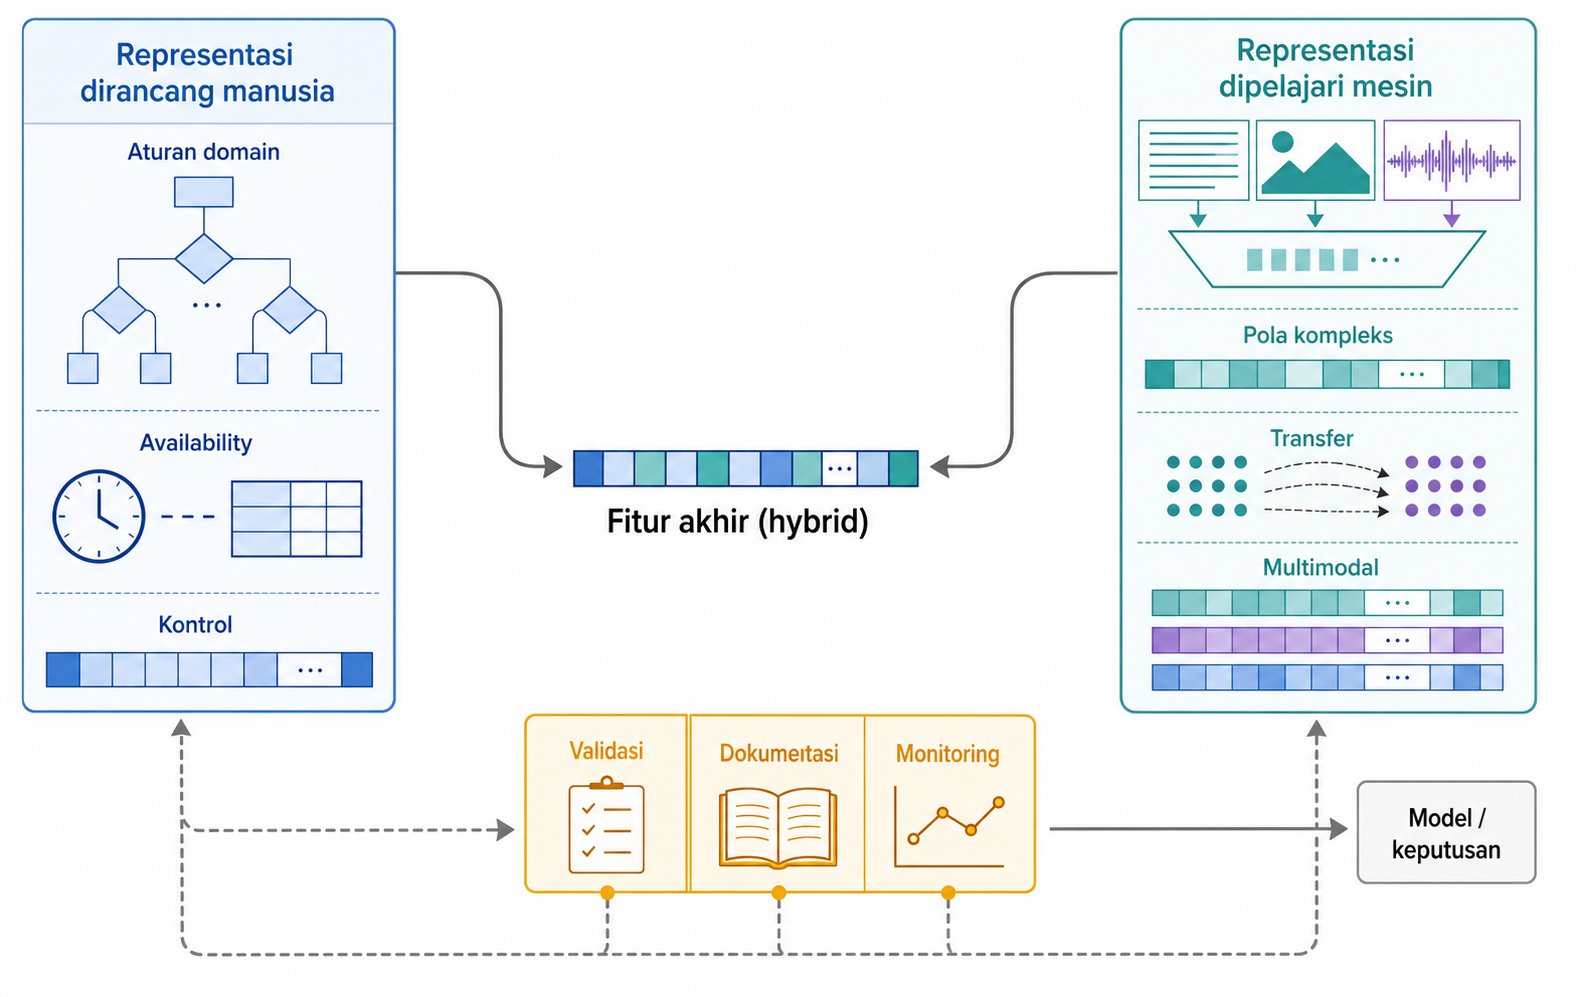
\includegraphics[width=111.6mm]{ch17-fig-4}
\caption{Representasi yang dirancang manusia dan representasi yang dipelajari mesin dalam satu \emph{pipeline}}
\label{fig:ch17-fig-4}
\end{figure}

Tabel 17.2 adalah checklist akhir. Ia dirancang untuk dibaca sebelum proyek dimulai, saat feature review, dan sebelum model masuk produksi. Setiap baris memaksa satu pertanyaan yang harus bisa dijawab dengan bukti, bukan rasa yakin.

\tabeljudul{Tabel 17.2 — Daftar periksa prinsip yang bertahan lama}

{\def\LTcaptype{none} % do not increment counter
\par\vspace{3pt}\noindent
\begingroup\renewcommand{\arraystretch}{1.0}%
\scriptsize\linespread{1}\selectfont
\renewcommand{\_}{\textunderscore\hspace{0pt}}%
\begin{xltabular}{\linewidth}{@{}>{\raggedright\arraybackslash}p{(\linewidth-2\tabcolsep)*\real{0.480}} >{\raggedright\arraybackslash}p{(\linewidth-2\tabcolsep)*\real{0.520}}@{}}
\toprule

Prinsip
 & 
Pertanyaan yang harus bisa dijawab
 \\
\midrule
\endhead




Mulai dari masalah & Apa unit, target, horizon, dan \emph{cutoff}? \\
Ketersediaan & Apakah fitur ini ada, segar, dan cukup cepat saat prediksi? \\
Transformasi mengikuti \emph{split} & Di mana transformasi ini di-fit, kapan dibekukan, dan ke mana diterapkan? \\
Kualitas melampaui importance & Apakah fitur tersedia, stabil, terjangkau, dan sah? \\
Validasi mengalahkan jumlah fitur & Apa \emph{baseline}-nya, dan apa bukti fitur ini menambah nilai? \\
Privasi dan proxy & Siapa yang bisa dirugikan, dan lewat jalur proxy apa? \\
Dokumentasi dan monitoring & Siapa pemilik fitur, versinya apa, dan bagaimana kita tahu ia masih bekerja? \\
\bottomrule
\end{xltabular}\endgroup\par\vspace{5pt}

}

Dokumentasi membuat rekayasa fitur tahan lama: definisi, sumber, \emph{cutoff}, risiko, versi, pemilik, dan monitor. Tanpa itu, fitur yang bagus hari ini menjadi hutang teknis besok. Dengan itu, fitur dapat dievaluasi ulang ketika data berubah, model berganti, atau aturan bisnis bergerak.

Jalan ke depan bersifat hybrid. Manusia merumuskan masalah, memilih batas, dan menilai konsekuensi. Mesin belajar representasi, mengusulkan kandidat, dan mempercepat pencarian. \emph{Pipeline} yang baik menyatukan keduanya di bawah validasi yang jujur. Dengan bahasa Bab 1, pekerjaan ini tetap tentang merancang \(\phi(x_{\text{raw}})\): transformasi dari data mentah ke representasi yang sah, berguna, dan dapat dipelihara. Setiap proyek ML/DL seharusnya dapat menjawab: representasi apa yang kita pilih, mengapa, dan bagaimana kita tahu ia bekerja?

\begin{bacaan}

\begin{itemize}
\tightlist
\item
  scikit-learn --- Common Pitfalls \& Pipelines --- \url{https://scikit-learn.org/stable/common_pitfalls.html}. Disiplin pipeline untuk produksi.
\item
  Sculley dkk. (2015), Hidden Technical Debt in ML Systems (NeurIPS) --- \url{https://papers.nips.cc/paper/2015/hash/86df7dcfd896fcaf2674f757a2463eba-Abstract.html}. Sumber sintesis utama untuk utang teknis ML.
\item
  Gebru dkk. (2021), Datasheets for Datasets --- \url{https://arxiv.org/abs/1803.09010}. Dokumentasi asal dan batasan data.
\item
  TensorFlow Data Validation --- \url{https://www.tensorflow.org/tfx/data_validation}. Validasi skema dan deteksi drift.
\item
  Great Expectations --- \url{https://greatexpectations.io/}. Uji kualitas data sebagai kode.
\item
  Evidently AI --- \url{https://docs.evidentlyai.com/}. Pemantauan drift data dan model.
\item
  Feast --- \url{https://docs.feast.dev/}. Feature store: konsistensi latih--saji.
\item
  ICO --- Data minimisation --- \url{https://ico.org.uk/for-organisations/uk-gdpr-guidance-and-resources/data-protection-principles/a-guide-to-the-data-protection-principles/the-principles/data-minimisation/}. Prinsip minimisasi data (privasi).
\end{itemize}

\end{bacaan}

\rujukanheading

\protect\phantomsection\label{refs}
\begin{CSLReferences}{1}{1}
\bibitem[\citeproctext]{ref-breck2017mltest}
Breck, Eric, Shanqing Cai, Eric Nielsen, Michael Salib, and D. Sculley. 2017. {``The {ML} Test Score: A Rubric for {ML} Production Readiness and Technical Debt Reduction.''} \emph{IEEE International Conference on Big Data}.

\bibitem[\citeproctext]{ref-gama2014driftsurvey}
Gama, João, Indrė Žliobaitė, Albert Bifet, Mykola Pechenizkiy, and Abdelhamid Bouchachia. 2014. {``A Survey on Concept Drift Adaptation.''} \emph{ACM Computing Surveys} 46 (4): 1--37.

\bibitem[\citeproctext]{ref-sculley2015debt}
Sculley, D., Gary Holt, Daniel Golovin, et al. 2015. {``Hidden Technical Debt in Machine Learning Systems.''} \emph{Advances in Neural Information Processing Systems (NeurIPS)}.

\end{CSLReferences}


% --- Lampiran (bab \appendix: penomoran bab jadi huruf A, B, C) ------------
\appendix
\renewcommand{\appendixname}{Lampiran}
% Kepala bab lampiran: kicker "LAMPIRAN A" (bukan angka 58pt seperti bab isi),
% lalu judul deskriptif Huge + garis, senada gaya bab tetapi jelas sebagai lampiran.
\titleformat{\chapter}[display]
  {\sffamily}
  {\flushright\large\bfseries\color{panelbar}\MakeUppercase{\appendixname\ \thechapter}}
  {2pt}
  {\Huge\bfseries\color{black}\raggedright}
  [\vspace{7pt}{\color{rulegray}\titlerule[1.4pt]}]
\titlespacing*{\chapter}{0pt}{6pt}{28pt}
% ==========================================================================
% lampiran-A.tex — dihasilkan dari lampiran/lampiran-A-peta-pemilihan-teknik.md oleh tools/lampiran2tex.py
% Boleh disunting manual; menjalankan lampiran2tex.py lagi akan menimpa.
% ==========================================================================
\chapter{Panduan Pemilihan Teknik}\label{panduan-pemilihan-teknik}

Lampiran ini merangkum keputusan rekayasa fitur yang tersebar di seluruh buku menjadi satu peta rujukan cepat. Lampiran tersebut tidak menggantikan pembahasan tiap bab, melainkan menjadi titik masuk. Temukan baris yang cocok dengan persoalan Anda, lalu buka bab yang dirujuk untuk memahami alasan di baliknya.

Pemilihan teknik representasi data pada praktiknya jarang ditentukan oleh satu faktor saja.
Empat sumbu berikut biasanya bekerja bersamaan: \textbf{tipe data} yang dihadapi,
\textbf{jenis model} yang akan dipakai, \textbf{ukuran data} yang tersedia, dan
\textbf{kebutuhan interpretabilitas} dari hasil akhir. Panduan ini memecah keempatnya
menjadi tabel terpisah agar mudah dibaca, dan ditutup dengan beberapa aturan
gabungan yang sering muncul.

\section{Berdasarkan tipe data}\label{berdasarkan-tipe-data}

Faktor paling menentukan. Tipe data menetapkan jenis representasi yang sesuai lebih dari faktor lainnya.

{\def\LTcaptype{none} % do not increment counter
\par\vspace{3pt}\noindent
\begingroup\renewcommand{\arraystretch}{1.0}%
\scriptsize\linespread{1}\selectfont
\renewcommand{\_}{\textunderscore\hspace{0pt}}%
\begin{xltabular}{\linewidth}{@{}>{\raggedright\arraybackslash}p{(\linewidth-6\tabcolsep)*\real{0.203}} >{\raggedright\arraybackslash}p{(\linewidth-6\tabcolsep)*\real{0.374}} >{\raggedright\arraybackslash}p{(\linewidth-6\tabcolsep)*\real{0.355}} >{\raggedright\arraybackslash}p{(\linewidth-6\tabcolsep)*\real{0.068}}@{}}
\toprule

Tipe data
 & 
Representasi awal yang lazim
 & 
Teknik lanjutan
 & 
Bab
 \\
\midrule
\endhead




Numerik kontinu & penskalaan (\emph{standardize}\slash{}\emph{min--max}), transformasi (\emph{log}, Box--Cox) & \emph{binning}, interaksi polinomial, \emph{clipping} & 3 \\
Kategorikal kardinalitas rendah & \emph{one-hot encoding} & \emph{ordinal} (bila ada urutan) & 4 \\
Kategorikal kardinalitas tinggi & \emph{target encoding} (dengan \emph{cross-fitting}), \emph{hashing} & \emph{entity embedding} & 4, 15 \\
Nilai hilang \slash{} \emph{outlier} & imputasi (di dalam \emph{pipeline}), penanda hilang & \emph{winsorizing}, model tahan-\emph{outlier} & 5 \\
Fitur turunan dari log\slash{}event & agregasi berjendela, \emph{as-of join} & rasio, \emph{recency}, fitur siklik & 6 \\
Deret waktu \slash{} sensor & \emph{lag}, \emph{rolling window}, fitur kalender & \emph{expanding window}, dekomposisi musiman & 10 \\
Teks \slash{} dokumen & \emph{bag-of-words}, TF-IDF & \emph{word\slash{}document embedding}, model \emph{pretrained} & 11, 15 \\
Citra & statistik piksel, HOG & fitur dari CNN \emph{pretrained}, \emph{patch embedding} & 12, 15 \\
Audio & MFCC, log-mel & \emph{embedding} audio \emph{pretrained} & 12 \\
Spasial (koordinat) & jarak geodesik, fitur radius, indeks grid (H3) & \emph{spatial lag}, autokorelasi & 13 \\
Graf \slash{} relasional & derajat, sentralitas & \emph{spectral embedding}, GNN & 13 \\
Multimodal & konkatenasi fitur per-modalitas & fusi terlambat (\emph{late fusion}), \emph{joint embedding} & 14 \\
\bottomrule
\end{xltabular}\endgroup\par\vspace{5pt}

}

\section{Berdasarkan jenis model}\label{berdasarkan-jenis-model}

Model yang berbeda menuntut prapemrosesan yang berbeda. Salah satu kolom yang utamanya perlu diperhatikan adalah ``sensitif skala'' dan ``butuh encoding''. Keduanya menentukan apakah prapemrosesan wajib atau bisa dilewati.

{\def\LTcaptype{none} % do not increment counter
\par\vspace{3pt}\noindent
\begingroup\renewcommand{\arraystretch}{1.0}%
\scriptsize\linespread{1}\selectfont
\renewcommand{\_}{\textunderscore\hspace{0pt}}%
\begin{xltabular}{\linewidth}{@{}>{\raggedright\arraybackslash}p{(\linewidth-8\tabcolsep)*\real{0.171}} >{\raggedright\arraybackslash}p{(\linewidth-8\tabcolsep)*\real{0.160}} >{\raggedright\arraybackslash}p{(\linewidth-8\tabcolsep)*\real{0.160}} >{\raggedright\arraybackslash}p{(\linewidth-8\tabcolsep)*\real{0.443}} >{\raggedright\arraybackslash}p{(\linewidth-8\tabcolsep)*\real{0.066}}@{}}
\toprule

Keluarga model
 & 
Sensitif skala?
 & 
Butuh encoding kategori?
 & 
Catatan rekayasa fitur
 & 
Bab
 \\
\midrule
\endhead




Linear \slash{} logistik & Ya & Ya (\emph{one-hot}\slash{}\emph{target}) & untung dari interaksi \& transformasi eksplisit; regularisasi (\emph{lasso}) sekaligus menyeleksi & 3, 4, 7 \\
k-NN, SVM (RBF) & Ya (kritis) & Ya & jarak rusak tanpa penskalaan; hati-hati dimensi tinggi & 3, 8 \\
Pohon \slash{} \emph{gradient boosting} & Tidak & Sebagian (bisa terima \emph{ordinal}) & tahan skala \& \emph{outlier}; fitur turunan tetap membantu & 6, 10 \\
Jaringan saraf (tabular) & Ya & \emph{embedding} untuk kategori & \emph{entity embedding} menggantikan \emph{one-hot} lebar & 15 \\
Model \emph{pretrained} (teks\slash{}citra) & ditangani model & tidak relevan & rekayasa fitur bergeser ke \emph{input representation} \& \emph{tokenization} & 15 \\
\bottomrule
\end{xltabular}\endgroup\par\vspace{5pt}

}

\section{Berdasarkan ukuran data}\label{berdasarkan-ukuran-data}

Jumlah baris menentukan seberapa ``mahal'' sebuah representasi terwujud, dan
kapan representasi yang dipelajari mesin mulai unggul dibandingkan fitur manual.

{\def\LTcaptype{none} % do not increment counter
\par\vspace{3pt}\noindent
\begingroup\renewcommand{\arraystretch}{1.0}%
\scriptsize\linespread{1}\selectfont
\renewcommand{\_}{\textunderscore\hspace{0pt}}%
\begin{xltabular}{\linewidth}{@{}>{\raggedright\arraybackslash}p{(\linewidth-4\tabcolsep)*\real{0.181}} >{\raggedright\arraybackslash}p{(\linewidth-4\tabcolsep)*\real{0.466}} >{\raggedright\arraybackslash}p{(\linewidth-4\tabcolsep)*\real{0.353}}@{}}
\toprule

Ukuran data
 & 
Panduan representasi
 & 
Yang dihindari
 \\
\midrule
\endhead




Kecil (ratusan--ribuan baris) & fitur ringkas \& dirancang manusia; regularisasi kuat; validasi silang & \emph{one-hot} kardinalitas tinggi; model dalam tanpa regularisasi \\
Menengah (puluhan ribu) & \emph{gradient boosting} + fitur turunan sering jadi \emph{baseline} kuat & \emph{embedding} mahal yang tak terbukti menang \\
Besar (ratusan ribu ke atas) & representasi yang dipelajari mesin mulai kompetitif; \emph{hashing} untuk kardinalitas tinggi & fitur manual yang tak terskala; kebocoran akibat pipeline manual \\
\bottomrule
\end{xltabular}\endgroup\par\vspace{5pt}

}

\begin{quote}
Heuristik ``puluhan ribu baris'' (Bab 15) diilustrasikan pada Covertype: pada
subset 50k, \emph{gradient boosting} masih mengungguli MLP terskala. Ukuran bukan
satu-satunya penentu, tetapi ukuran data menggeser titik keseimbangan antara fitur
dirancang manusia dan dipelajari mesin.
\end{quote}

\section{Berdasarkan kebutuhan interpretabilitas}\label{berdasarkan-kebutuhan-interpretabilitas}

Bila keputusan harus dijelaskan (regulasi, audit, kepercayaan pemangku
kepentingan), representasi yang lebih transparan lebih penting daripada
sedikit kenaikan performa.

{\def\LTcaptype{none} % do not increment counter
\par\vspace{3pt}\noindent
\begingroup\renewcommand{\arraystretch}{1.0}%
\scriptsize\linespread{1}\selectfont
\renewcommand{\_}{\textunderscore\hspace{0pt}}%
\begin{xltabular}{\linewidth}{@{}>{\raggedright\arraybackslash}p{(\linewidth-4\tabcolsep)*\real{0.226}} >{\raggedright\arraybackslash}p{(\linewidth-4\tabcolsep)*\real{0.520}} >{\raggedright\arraybackslash}p{(\linewidth-4\tabcolsep)*\real{0.254}}@{}}
\toprule

Kebutuhan interpretabilitas
 & 
Representasi yang cocok
 & 
Representasi yang dihindari
 \\
\midrule
\endhead




Tinggi (harus dijelaskan) & fitur bermakna \& bernama; \emph{one-hot}\slash{}\emph{ordinal}; koefisien linear; \emph{importance} fitur & \emph{embedding} laten; komponen PCA tanpa makna \\
Sedang & fitur turunan terdokumentasi + model pohon dengan \emph{importance} & fusi multimodal buram \\
Rendah (skor diutamakan) & \emph{embedding} padat, representasi \emph{pretrained}, komponen laten & --- \\
\bottomrule
\end{xltabular}\endgroup\par\vspace{5pt}

}

\section{Aturan gabungan yang sering muncul}\label{aturan-gabungan-yang-sering-muncul}

Beberapa kombinasi lintas-faktor juga layak dijadikan perhatian:

\begin{enumerate}
\def\labelenumi{\arabic{enumi}.}
\tightlist
\item
  \textbf{k-NN atau model berbasis jarak + fitur berskala beragam → wajib penskalaan
  lebih dahulu.} Tanpa itu, satu fitur berskala besar mendominasi jarak (Bab 3).
\item
  \textbf{Kategori kardinalitas tinggi + model linear → \emph{target encoding} dengan
  \emph{cross-fitting}, bukan \emph{one-hot} lebar.} Tanpa \emph{cross-fitting}, muncul
  kebocoran halus (Bab 4).
\item
  \textbf{Data event/log + target masa depan → agregasi berjendela dengan \emph{cutoff}
  eksplisit dan \emph{as-of join}.} Ini penjaga kausalitas sekaligus anti-kebocoran
  (Bab 6, 10).
\item
  \textbf{Deret waktu → selalu \emph{split} menurut waktu, bukan acak.} \emph{Purge gap} bila
  ada \emph{horizon} target (Bab 10).
\item
  \textbf{Interpretabilitas tinggi + kardinalitas tinggi → pertimbangkan \emph{hashing}
  atau pengelompokan bermakna, dan dokumentasikan.} Hindari \emph{embedding} laten
  yang sulit dijelaskan (Bab 4, 9).
\item
  \textbf{Data besar + banyak kandidat fitur → otomasi pembangkitan fitur (DFS/AutoML)
  tetap butuh kurasi manusia.} Fitur yang plausibel bisa tetap \emph{spurious}
  (Bab 16).
\end{enumerate}

\begin{quote}
\textbf{Prasyarat lintas jalur:} apa pun tipe data Anda, Bab 2 (\emph{pipeline},
validasi, \emph{leakage}) dan Bab 9 (evaluasi kualitas fitur) tetap berlaku.
Panduan ini memilih \emph{representasi}. Kedua bab itu memastikan representasi tersebut sah dan terukur. Istilah asing pada tabel di atas dijelaskan ringkas di
\textbf{Lampiran B (Glosarium)}.
\end{quote}

% ==========================================================================
% lampiran-B.tex — dihasilkan dari lampiran/lampiran-B-glosarium.md oleh tools/lampiran2tex.py
% Boleh disunting manual; menjalankan lampiran2tex.py lagi akan menimpa.
% ==========================================================================
\chapter{Glosarium}\label{glosarium}

Daftar istilah beserta padanan Inggris dan penjelasan ringkas. Mengikuti kebijakan istilah buku: pakai kata Indonesia yang memang lazim di komunitas TI/ilmu komputer; bila tidak ada, pertahankan istilah Inggris (dicetak \emph{miring}). Definisi di sini sengaja singkat --- untuk pembahasan penuh, lihat bab yang dirujuk.

Format tiap entri: \textbf{istilah (Indonesia / Inggris)} --- penjelasan ringkas \emph{(Bab)}.

\glosletter{A}

\textbf{Agregasi berjendela / \emph{windowed aggregation}} --- meringkas banyak event menjadi
satu nilai fitur dalam rentang waktu tertentu sebelum titik acuan (mis. total
transaksi 90 hari terakhir). \emph{(Bab 6, 10)}

\textbf{Anti-kebocoran / \emph{leakage prevention}} --- praktik memastikan tidak ada
informasi dari masa depan atau dari data uji yang bocor ke fitur saat pelatihan.
\emph{(Bab 2)}

\textbf{\emph{As-of join}} --- penggabungan tabel yang hanya mengambil informasi yang tersedia
\emph{sebelum} waktu acuan, menjaga kausalitas. \emph{(Bab 6)}

\textbf{Atribut / \emph{attribute}} --- kolom mentah pada data sebelum diolah menjadi fitur.
\emph{(Bab 1)}

\textbf{\emph{Autoencoder}} --- jaringan yang belajar memampatkan data ke representasi laten
lalu merekonstruksinya; dipakai untuk reduksi dimensi non-linear. \emph{(Bab 8)}

\textbf{Autokorelasi spasial / \emph{spatial autocorrelation}} --- kecenderungan nilai di
lokasi berdekatan lebih mirip daripada lokasi berjauhan (hukum pertama geografi
Tobler). \emph{(Bab 13)}

\glosletter{B}

\textbf{\emph{Bag-of-words} (BoW)} --- representasi teks sebagai hitungan kemunculan kata,
mengabaikan urutan. \emph{(Bab 11)}

\textbf{\emph{Baseline}} --- model atau representasi pembanding sederhana yang menjadi tolok
ukur; kenaikan skor diukur relatif terhadapnya. \emph{(Bab 9)}

\textbf{\emph{Batch}} --- sekumpulan sampel yang diproses bersama dalam satu langkah
pelatihan. \emph{(Bab 15)}

\textbf{\emph{Binning}} --- mengubah fitur numerik kontinu menjadi kategori bertingkat
(\emph{bin}); dapat menghilangkan sebagian informasi. \emph{(Bab 3)}

\glosletter{C}

\textbf{\emph{Clipping}} --- memotong nilai ekstrem ke batas atas/bawah yang ditetapkan untuk
meredam pengaruh \emph{outlier}. \emph{(Bab 3, 5)}

\textbf{\emph{Cross-fitting}} --- menghitung \emph{encoding} atau statistik pada lipatan data yang
berbeda dari yang diterapkan, mencegah kebocoran pada \emph{target encoding}. \emph{(Bab 4)}

\textbf{\emph{Cutoff} (waktu prediksi)} --- titik waktu acuan yang memisahkan informasi yang
boleh dipakai (masa lalu) dari yang harus diprediksi (masa depan). \emph{(Bab 6, 10)}

\glosletter{D}

\textbf{\emph{Data leakage}} --- masuknya informasi yang seharusnya tak tersedia saat
\emph{inference} ke dalam fitur pelatihan, membuat skor validasi terlalu optimistis.
\emph{(Bab 2)}

\textbf{\emph{Deep learning}} --- pembelajaran dengan jaringan saraf berlapis banyak yang
mampu belajar representasi bertingkat dari data. \emph{(Bab 15)}

\textbf{Deret waktu / \emph{time series}} --- data yang terurut menurut waktu, dengan
ketergantungan antar-waktu yang harus dijaga saat validasi. \emph{(Bab 10)}

\textbf{Dimensi / \emph{dimension}} --- jumlah fitur (kolom) yang merepresentasikan tiap
sampel. \emph{(Bab 8)}

\textbf{Distribusi / \emph{distribution}} --- pola sebaran nilai sebuah fitur; bentuknya
(\emph{skew}, ekor tebal) memengaruhi pilihan transformasi. \emph{(Bab 3)}

\glosletter{E}

\textbf{\emph{Embedding}} --- representasi padat berdimensi rendah yang menempatkan objek
serupa saling berdekatan dalam ruang vektor. \emph{(Bab 11, 15)}

\textbf{\emph{Encoding}} --- proses mengubah kategori menjadi angka yang dapat diolah model.
\emph{(Bab 4)}

\textbf{\emph{Entity embedding}} --- \emph{embedding} yang dipelajari untuk nilai-nilai kategori,
alternatif padat bagi \emph{one-hot} pada kardinalitas tinggi. \emph{(Bab 4, 15)}

\textbf{\emph{Epoch}} --- satu kali lintasan penuh atas seluruh data pelatihan. \emph{(Bab 15)}

\textbf{\emph{Expanding window}} --- jendela agregasi yang tumbuh dari awal riwayat sampai
titik acuan (berbeda dari \emph{rolling} yang lebarnya tetap). \emph{(Bab 10)}

\glosletter{F}

\textbf{\emph{Feature extractor}} --- model \emph{pretrained} yang lapisan-lapisannya dipakai untuk
menghasilkan fitur, tanpa dilatih ulang. \emph{(Bab 15)}

\textbf{\emph{Feature store}} --- sistem penyimpanan fitur terpusat agar konsisten antara
pelatihan dan \emph{inference}. \emph{(Bab 17)}

\textbf{\emph{Fine-tuning}} --- melanjutkan pelatihan model \emph{pretrained} pada data tugas
tertentu untuk mengadaptasinya. \emph{(Bab 15)}

\textbf{Fitur / \emph{feature}} --- besaran hasil rekayasa yang menjadi masukan model;
istilah rumah buku ini. \emph{(Bab 1)}

\textbf{Fitur turunan / \emph{derived feature}} --- fitur baru yang dibentuk dari satu atau
lebih atribut mentah (rasio, selisih, agregat). \emph{(Bab 6)}

\glosletter{G}

\textbf{\emph{Gradient}} --- arah dan besar perubahan galat terhadap parameter; dasar
optimasi model. \emph{(Bab 15)}

\textbf{\emph{Gradient boosting}} --- ansambel pohon yang dibangun bertahap; kuat pada data
tabular dan tahan terhadap skala serta \emph{outlier}. \emph{(Bab 6, 15)}

\textbf{Graf / \emph{graph}} --- data berupa simpul (\emph{node}) dan sisi (\emph{edge}) yang
merepresentasikan relasi. \emph{(Bab 13)}

\textbf{\emph{Graph neural network} (GNN)} --- jaringan yang belajar representasi simpul lewat
\emph{message passing} dari tetangga di graf. \emph{(Bab 13)}

\glosletter{H}

\textbf{\emph{Hashing (trick)}} --- memetakan kategori ke indeks tetap lewat fungsi \emph{hash},
menekan dimensi pada kardinalitas sangat tinggi dengan risiko kolisi. \emph{(Bab 4)}

\textbf{HOG (\emph{Histogram of Oriented Gradients})} --- deskriptor citra berbasis distribusi
arah gradien lokal. \emph{(Bab 12)}

\textbf{\emph{Horizon}} --- rentang waktu ke depan yang menjadi sasaran prediksi, dihitung
dari \emph{cutoff}. \emph{(Bab 10)}

\glosletter{I}

\textbf{Imputasi / \emph{imputation}} --- mengisi nilai hilang dengan estimasi (rata-rata,
median, model); harus dihitung di dalam \emph{pipeline} agar tak bocor. \emph{(Bab 5)}

\textbf{\emph{Inference}} --- tahap pemakaian model pada data baru; fitur harus tersedia pada
saat ini. \emph{(Bab 2, 17)}

\textbf{\emph{Input}} --- data yang masuk ke model; bentuknya ditentukan oleh rekayasa fitur.
\emph{(Bab 1)}

\textbf{Interpretabilitas / \emph{interpretability}} --- sejauh mana keputusan model dapat
dijelaskan; sering bergantung pada kebermaknaan fitur. \emph{(Bab 9)}

\glosletter{K}

\textbf{Kardinalitas / \emph{cardinality}} --- banyaknya nilai unik pada fitur kategorikal;
menentukan strategi \emph{encoding}. \emph{(Bab 4)}

\textbf{Kebocoran} --- lihat \textbf{\emph{Data leakage}}.

\glosletter{L}

\textbf{\emph{Lag}} --- nilai fitur atau target dari langkah waktu sebelumnya, dipakai sebagai
fitur pada deret waktu. \emph{(Bab 10)}

\textbf{\emph{Lasso} (regularisasi L1)} --- regularisasi yang menyusutkan sebagian koefisien
tepat ke nol, sekaligus menyeleksi fitur. \emph{(Bab 7)}

\textbf{\emph{Late fusion} / fusi terlambat} --- menggabungkan keluaran (skor) dari model
per-modalitas, bukan menyatukan fiturnya lebih awal. \emph{(Bab 14)}

\textbf{\emph{Machine learning}} --- pembelajaran pola dari data untuk membuat prediksi tanpa
aturan yang diprogram eksplisit. \emph{(Bab 1)}

\glosletter{M}

\textbf{MFCC (\emph{Mel-Frequency Cepstral Coefficients})} --- fitur audio ringkas yang lazim
untuk pengenalan suara. \emph{(Bab 12)}

\textbf{\emph{Missing value} / nilai hilang} --- sel data yang tidak terisi; polanya (acak
atau terstruktur) memengaruhi penanganan. \emph{(Bab 5)}

\textbf{Multimodal} --- data yang memadukan lebih dari satu modalitas (mis. teks +
citra + tabular). \emph{(Bab 14)}

\glosletter{N}

\textbf{NMF (\emph{Non-negative Matrix Factorization})} --- pemfaktoran matriks non-negatif
menjadi komponen aditif yang sering lebih mudah ditafsir. \emph{(Bab 8)}

\textbf{\emph{Noise} / \emph{derau}} --- variasi acak tak bermakna pada data; buku memakai istilah
\emph{noise}. \emph{(Bab 3)}

\glosletter{O}

\textbf{\emph{One-hot encoding}} --- merepresentasikan kategori sebagai vektor biner dengan
satu posisi bernilai 1; menjaga kategori terpisah tetapi memperlebar matriks.
\emph{(Bab 4)}

\textbf{\emph{Ordinal encoding}} --- memberi kategori kode angka berurut; hemat dimensi tetapi
memaksakan asumsi urutan. \emph{(Bab 4)}

\textbf{\emph{Outlier}} --- nilai yang menyimpang jauh dari sebaran umum; dapat mengganggu
model sensitif skala. \emph{(Bab 5)}

\textbf{\emph{Overfitting}} --- model terlalu menyesuaikan data latih hingga gagal
menggeneralisasi ke data baru. \emph{(Bab 7, 9)}

\glosletter{P}

\textbf{\emph{Pipeline}} --- rangkaian langkah praproses dan model yang dijalankan sebagai satu
kesatuan; kunci agar transformasi mengikuti pembagian data. \emph{(Bab 2)}

\textbf{Praktik pipeline yang benar / \emph{pipeline discipline}} --- kebiasaan memasang
semua transformasi di dalam \emph{pipeline} sehingga di-\emph{fit} hanya pada data latih.
\emph{(Bab 2)}

\textbf{\emph{Pretrained} (model)} --- model yang sudah dilatih pada data besar dan dipakai
kembali sebagai sumber representasi. \emph{(Bab 15)}

\textbf{\emph{Purge gap}} --- jeda yang sengaja dikosongkan antara periode latih dan uji pada
\emph{split} temporal untuk mencegah kebocoran lewat \emph{horizon}. \emph{(Bab 10)}

\glosletter{R}

\textbf{\emph{Recency}} --- fitur yang mengukur seberapa baru event terakhir relatif terhadap
\emph{cutoff}. \emph{(Bab 6)}

\textbf{Reduksi dimensi / \emph{dimensionality reduction}} --- memampatkan banyak fitur
menjadi sedikit sambil mempertahankan informasi penting. \emph{(Bab 8)}

\textbf{Regularisasi / \emph{regularization}} --- penalti pada kompleksitas model untuk
menekan \emph{overfitting}. \emph{(Bab 7)}

\textbf{Rekayasa fitur / \emph{feature engineering}} --- disiplin merancang representasi data
yang sah, bermanfaat, dan dapat digunakan kembali; tema utama buku ini. \emph{(Bab 1)}

\textbf{Representasi / \emph{representation}} --- bentuk data yang disajikan kepada model;
menentukan pola apa yang dapat dipelajari. \emph{(Bab 1)}

\textbf{Representasi yang dipelajari mesin / \emph{learned representation}} --- fitur yang
dipelajari otomatis oleh model (mis. \emph{embedding}), bukan dirancang tangan.
\emph{(Bab 15)}

\textbf{Representasi yang dirancang manusia / \emph{designed representation}} --- fitur yang
dibentuk secara sengaja oleh perancang berdasarkan pemahaman domain. \emph{(Bab 1, 6)}

\textbf{\emph{Rolling window}} --- jendela agregasi berlebar tetap yang bergeser di sepanjang
waktu. \emph{(Bab 10)}

\glosletter{S}

\textbf{Sarat informasi / \emph{information-rich}} --- sifat data/log/tabel yang memuat
banyak sinyal berguna. \emph{(Bab 1)}

\textbf{Seleksi fitur / \emph{feature selection}} --- memilih himpunan bagian fitur yang
relevan (metode \emph{filter}, \emph{wrapper}, \emph{embedded}). \emph{(Bab 7)}

\textbf{Skala / \emph{scale}} --- rentang nilai sebuah fitur; perbedaan skala antar-fitur
merusak model berbasis jarak bila tak disamakan. \emph{(Bab 3)}

\textbf{\emph{Spatial lag}} --- rata-rata berbobot nilai tetangga sebuah lokasi, dipakai
sebagai fitur spasial. \emph{(Bab 13)}

\textbf{\emph{Spectral embedding}} --- representasi simpul graf dari vektor eigen matriks graf.
\emph{(Bab 13)}

\textbf{Standardisasi / \emph{standardization}} --- penskalaan agar fitur bermean 0 dan
berdeviasi baku 1. \emph{(Bab 3)}

\glosletter{T}

\textbf{\emph{Target encoding}} --- menggantikan kategori dengan statistik target (mis.
rata-rata) yang terkait; kuat pada kardinalitas tinggi tetapi rawan bocor tanpa
\emph{cross-fitting}. \emph{(Bab 4)}

\textbf{\emph{Target} / sasaran} --- besaran yang ingin diprediksi model. \emph{(Bab 1)}

\textbf{TF-IDF (\emph{Term Frequency--Inverse Document Frequency})} --- pembobotan kata yang
menaikkan istilah khas dokumen dan menurunkan istilah umum. \emph{(Bab 11)}

\textbf{\emph{Tokenization} / tokenisasi} --- memecah teks menjadi satuan (\emph{token}) sebelum
divektorkan. \emph{(Bab 11, 15)}

\textbf{\emph{Training--inference skew} / \emph{training--serving skew}} --- ketidaksesuaian cara
fitur dihitung saat pelatihan versus saat \emph{inference}. \emph{(Bab 17)}

\textbf{Transformasi (fitur numerik)} --- pengubahan bentuk distribusi (mis. \emph{log},
\emph{Box--Cox}) agar lebih sesuai untuk model. \emph{(Bab 3)}

\glosletter{V}

\textbf{Validasi silang / \emph{cross-validation}} --- membagi data menjadi beberapa lipatan
untuk menilai generalisasi; variannya (\emph{Group}, \emph{TimeSeries}) menjaga struktur
data. \emph{(Bab 2, 9)}

\textbf{Vektor \emph{sparse} / \emph{sparse vector}} --- vektor yang sebagian besar elemennya nol,
khas representasi teks \emph{bag-of-words}/TF-IDF. \emph{(Bab 11)}

\glosletter{W}

\textbf{\emph{Winsorizing}} --- mengganti nilai ekstrem dengan persentil tertentu alih-alih
membuangnya. \emph{(Bab 5)}

\textbf{\emph{Word embedding}} --- \emph{embedding} untuk kata yang menangkap kedekatan makna
(mis. \emph{word2vec}). \emph{(Bab 11, 15)}

\begin{quote}
\textbf{Catatan penggunaan istilah.} Beberapa padanan Indonesia purist sengaja
dihindari karena tidak lazim di komunitas: \emph{derau} (dipakai: \emph{noise}), \emph{larik}
(\emph{array}), \emph{daring} (\emph{online}), \emph{masukan} untuk input model (dipakai: \emph{input}).
Kata \textbf{fitur} dipakai konsisten sebagai padanan \emph{feature}.
\end{quote}

% ==========================================================================
% lampiran-C.tex — dihasilkan dari lampiran/lampiran-C-matriks-dataset-bab.md oleh tools/lampiran2tex.py
% Boleh disunting manual; menjalankan lampiran2tex.py lagi akan menimpa.
% ==========================================================================
\chapter{Matriks Dataset × Bab}\label{matriks-dataset-bab}

Daftar dataset kurasi yang dipakai di seluruh buku: di bab mana muncul, dan untuk memperlihatkan hal apa (\emph{axis} pengajaran). Berguna sebagai alat perencanaan penggunaan kembali saat menulis, sekaligus rujukan bagi pembaca yang ingin menelusuri satu data sepanjang pipeline. Detail unduhan, versi, dan snapshot ada di repositori. Lampiran ini hanya berfungsi sebagai penunjuk.

\section{Matriks ringkas}\label{matriks-ringkas}

{\def\LTcaptype{none} % do not increment counter
\par\vspace{3pt}\noindent
\begingroup\renewcommand{\arraystretch}{1.0}%
\scriptsize\linespread{1}\selectfont
\renewcommand{\_}{\textunderscore\hspace{0pt}}%
\begin{xltabular}{\linewidth}{@{}>{\raggedright\arraybackslash}p{(\linewidth-6\tabcolsep)*\real{0.248}} >{\raggedright\arraybackslash}p{(\linewidth-6\tabcolsep)*\real{0.072}} >{\raggedright\arraybackslash}p{(\linewidth-6\tabcolsep)*\real{0.520}} >{\raggedright\arraybackslash}p{(\linewidth-6\tabcolsep)*\real{0.160}}@{}}
\toprule

Dataset
 & 
Bab
 & 
Axis yang diperlihatkan
 & 
Lisensi
 \\
\midrule
\endhead




UCI Online Retail & 1, 2, 6, 16 & log event nyata: unit\slash{}target\slash{}\emph{cutoff}, \emph{split} grup \& waktu, agregasi berjendela, audit fitur otomatis & CC BY 4.0 \\
UCI Online News Popularity & 3 & skala \& skew numerik heterogen; efek standardisasi pada k-NN & CC BY 4.0 \\
UCI Census-Income (KDD) & 4 & kardinalitas kategori beragam; kategori tak dikenal (\emph{split} 1994→1995) & CC BY 4.0 \\
UCI Communities and Crime & 5 & \emph{missingness} terstruktur (blok kolom LEMAS); ekor \& \emph{outlier} & CC BY 4.0 \\
UCI Breast Cancer Wisconsin (WDBC) & 7, 9 & fitur redundan berkorelasi tinggi: seleksi fitur \& ablasi\slash{}permutasi & CC BY 4.0 \\
Optical Recognition of Handwritten Digits & 8 & matriks piksel non-negatif: PCA\slash{}SVD\slash{}t-SNE\slash{}UMAP \& NMF & CC BY 4.0 \\
UCI Bike Sharing & 10 & musiman jam\slash{}pekan: \emph{lag}, \emph{rolling}, \emph{split} temporal \& kebocoran \emph{future} & CC BY 4.0 \\
UCI SMS Spam Collection & 11, 15 & teks sparse, imbalans kelas, duplikat: BoW\slash{}TF-IDF \& \emph{embedding} & CC BY 4.0 \\
Fashion-MNIST & 12, 15 & citra grayscale: HOG vs \emph{embedding} PCA piksel; ekstraksi fitur & MIT \\
Free Spoken Digit Dataset (FSDD) & 12, 15 & audio: MFCC vs log-mel; peringatan \emph{holdout} penutur & CC BY-SA 4.0 \\
Meuse (\passthrough{\lstinline!sp!}, CRAN) & 13 & koordinat spasial: autokorelasi, \emph{spatial lag}, blok CV vs acak & GPL (≥ 2) \\
Zachary Karate Club (NetworkX) & 13 & graf sosial: sentralitas \& \emph{spectral embedding}, sisi lintas-\emph{split} & BSD-3-Clause \\
Open Food Facts (subset) & 14 & multimodal selaras (teks + tabular + citra): fusi \& \emph{joint embedding} & ODbL \slash{} CC BY-SA \\
UCI Covertype (subset 50k) & 15 & skala tabular besar: \emph{gradient boosting} vs MLP (heuristik ``puluhan ribu baris'') & CC BY 4.0 \\
\bottomrule
\end{xltabular}\endgroup\par\vspace{5pt}

}

\emph{Bab 17 (Sintesis) tidak memakai dataset baru. Bab tersebut merangkai kembali contoh dari
bab-bab sebelumnya.}

\section{Dua data yang digunakan sepanjang pipeline}\label{dua-data-yang-digunakan-sepanjang-pipeline}

Sebagian dataset sengaja dipakai ulang di beberapa bab agar pembaca dapat
melihat \textbf{satu data yang sama} melewati tahap pipeline yang berbeda:

\begin{itemize}
\tightlist
\item
  \textbf{UCI Online Retail (Bab 1 → 2 → 6 → 16).} Dari log transaksi mentah yang
  sama: Bab 1 memperkenalkan unit observasi, target, dan \emph{cutoff}; Bab 2
  memakainya untuk \emph{split} grup (per-\passthrough{\lstinline!CustomerID!}) dan waktu; Bab 6 membentuk
  fitur turunan berjendela dan \emph{as-of join}; Bab 16 mengaudit fitur yang
  dibangkitkan otomatis di atasnya. Ini contoh terbaik ``satu data sepanjang
  pipeline tabular''.
\item
  \textbf{WDBC (Bab 7 → 9).} Dataset diagnosis yang sama menopang dua sudut evaluasi:
  Bab 7 untuk seleksi fitur (dengan probe sintetis), Bab 9 untuk ablasi
  kelompok, importansi permutasi, dan importansi berbasis model.
\end{itemize}

\section{Data yang dibagi antar-modalitas di Bab 15}\label{data-yang-dibagi-antar-modalitas-di-bab-15}

Bab 15 sengaja \textbf{tidak} memperkenalkan data teks/citra baru. Bab tersebut memakai ulang
SMS Spam (Bab 11) dan Fashion-MNIST/FSDD (Bab 12) untuk ekstraksi \emph{embedding},
lalu menambahkan \textbf{Covertype} hanya untuk perbandingan skala tabular. Dengan
begitu, fokus Bab 15 tetap pada representasi yang dipelajari mesin, bukan pada
pengenalan dataset.

\section{Catatan pemakaian}\label{catatan-pemakaian}

\begin{itemize}
\tightlist
\item
  \textbf{Semua dataset nyata} (bukan sintetis), dengan lisensi yang memperbolehkan
  penggunaan kembali. Probe sintetis pada Bab 7 dibangkitkan hanya di dalam demo notebook, bukan bagian identitas dataset.
\item
  \textbf{Angka baris/versi} merujuk pada \emph{frozen snapshot} di repositori, yang bisa
  sedikit berbeda dari jumlah yang ditampilkan halaman sumber saat ini
  (mis. Bike Sharing 17.379 baris pada snapshot vs 17.389 di halaman UCI). Untuk
  klaim di notebook, gunakan hitungan snapshot.
\item
  \textbf{Konten berada di repositori.} Dataset, versi \emph{library}, dan skrip praproses
  dapat diperbarui pasca-terbit tanpa cetak ulang. Buku berperan sebagai indeks
  stabil, sedangkan repositori sebagai konten yang bergerak.
\end{itemize}


% --- Bagian belakang ------------------------------------------------------
\backmatter
% ==========================================================================
% daftar-pustaka.tex — master bibliografi, dibangkitkan oleh tools/make_biblio.py
% Jangan sunting manual; sunting references.bib lalu jalankan ulang.
% ==========================================================================
\chapter*{Daftar Pustaka}
\addcontentsline{toc}{chapter}{Daftar Pustaka}
\markboth{Daftar Pustaka}{}

\protect\phantomsection\label{refs}
\begin{CSLReferences}{1}{1}
\bibitem[\citeproctext]{ref-alain2017probes}
Alain, Guillaume, and Yoshua Bengio. 2017. \emph{Understanding Intermediate Layers Using Linear Classifier Probes}. \url{https://arxiv.org/abs/1610.01644}.

\bibitem[\citeproctext]{ref-amershi2014power}
Amershi, Saleema, Maya Cakmak, W. Bradley Knox, and Todd Kulesza. 2014. {``Power to the People: The Role of Humans in Interactive Machine Learning.''} \emph{AI Magazine} 35 (4): 105--20.

\bibitem[\citeproctext]{ref-baevski2020wav2vec2}
Baevski, Alexei, Henry Zhou, Abdelrahman Mohamed, and Michael Auli. 2020. {``Wav2vec 2.0: A Framework for Self-Supervised Learning of Speech Representations.''} \emph{Advances in Neural Information Processing Systems (NeurIPS)}.

\bibitem[\citeproctext]{ref-baltrusaitis2019multimodal}
Baltrušaitis, Tadas, Chaitanya Ahuja, and Louis-Philippe Morency. 2019. {``Multimodal Machine Learning: A Survey and Taxonomy.''} \emph{IEEE Transactions on Pattern Analysis and Machine Intelligence} 41 (2): 423--43.

\bibitem[\citeproctext]{ref-barocas2016disparate}
Barocas, Solon, and Andrew D. Selbst. 2016. {``Big Data's Disparate Impact.''} \emph{California Law Review} 104: 671--732.

\bibitem[\citeproctext]{ref-bergmeir2012cv}
Bergmeir, Christoph, and José M. Benítez. 2012. {``On the Use of Cross-Validation for Time Series Predictor Evaluation.''} \emph{Information Sciences} 191: 192--213.

\bibitem[\citeproctext]{ref-bommasani2021foundation}
{Bommasani, Rishi, Drew A. Hudson, Ehsan Adeli, et al.} 2021. \emph{On the Opportunities and Risks of Foundation Models}. \url{https://arxiv.org/abs/2108.07258}.

\bibitem[\citeproctext]{ref-boxcox1964}
Box, George E. P., and David R. Cox. 1964. {``An Analysis of Transformations.''} \emph{Journal of the Royal Statistical Society, Series B} 26 (2): 211--52.

\bibitem[\citeproctext]{ref-breck2017mltest}
Breck, Eric, Shanqing Cai, Eric Nielsen, Michael Salib, and D. Sculley. 2017. {``The {ML} Test Score: A Rubric for {ML} Production Readiness and Technical Debt Reduction.''} \emph{IEEE International Conference on Big Data}.

\bibitem[\citeproctext]{ref-breiman2001randomforests}
Breiman, Leo. 2001. {``Random Forests.''} \emph{Machine Learning} 45 (1): 5--32.

\bibitem[\citeproctext]{ref-vanbuuren2011mice}
Buuren, Stef van, and Karin Groothuis-Oudshoorn. 2011. {``{mice}: Multivariate Imputation by Chained Equations in {R}.''} \emph{Journal of Statistical Software} 45 (3): 1--67.

\bibitem[\citeproctext]{ref-cawley2010overfitting}
Cawley, Gavin C., and Nicola L. C. Talbot. 2010. {``On over-Fitting in Model Selection and Subsequent Selection Bias in Performance Evaluation.''} \emph{Journal of Machine Learning Research} 11: 2079--107.

\bibitem[\citeproctext]{ref-chen2020simclr}
Chen, Ting, Simon Kornblith, Mohammad Norouzi, and Geoffrey Hinton. 2020. {``A Simple Framework for Contrastive Learning of Visual Representations.''} \emph{Proceedings of the 37th International Conference on Machine Learning (ICML)}. \url{https://arxiv.org/abs/2002.05709}.

\bibitem[\citeproctext]{ref-dalal2005hog}
Dalal, Navneet, and Bill Triggs. 2005. {``Histograms of Oriented Gradients for Human Detection.''} \emph{IEEE Conference on Computer Vision and Pattern Recognition (CVPR)}.

\bibitem[\citeproctext]{ref-devlin2019bert}
Devlin, Jacob, Ming-Wei Chang, Kenton Lee, and Kristina Toutanova. 2019. {``{BERT}: Pre-Training of Deep Bidirectional Transformers for Language Understanding.''} \emph{Proceedings of the 2019 Conference of the North American Chapter of the Association for Computational Linguistics (NAACL-HLT)}.

\bibitem[\citeproctext]{ref-erickson2020autogluon}
Erickson, Nick, Jonas Mueller, Alexander Shirkov, et al. 2020. \emph{{AutoGluon-Tabular}: Robust and Accurate {AutoML} for Structured Data}. \url{https://arxiv.org/abs/2003.06505}.

\bibitem[\citeproctext]{ref-feurer2015autosklearn}
Feurer, Matthias, Aaron Klein, Katharina Eggensperger, Jost Springenberg, Manuel Blum, and Frank Hutter. 2015. {``Efficient and Robust Automated Machine Learning.''} \emph{Advances in Neural Information Processing Systems (NeurIPS)}.

\bibitem[\citeproctext]{ref-gama2014driftsurvey}
Gama, João, Indrė Žliobaitė, Albert Bifet, Mykola Pechenizkiy, and Abdelhamid Bouchachia. 2014. {``A Survey on Concept Drift Adaptation.''} \emph{ACM Computing Surveys} 46 (4): 1--37.

\bibitem[\citeproctext]{ref-grill2020byol}
{Grill, Jean-Bastien, Florian Strub, Florent Altché, Corentin Tallec, Pierre H. Richemond, et al.} 2020. {``Bootstrap Your Own Latent: A New Approach to Self-Supervised Learning.''} \emph{Advances in Neural Information Processing Systems (NeurIPS)}. \url{https://arxiv.org/abs/2006.07733}.

\bibitem[\citeproctext]{ref-groverleskovec2016}
Grover, Aditya, and Jure Leskovec. 2016. {``Node2vec: Scalable Feature Learning for Networks.''} \emph{Proceedings of the 22nd ACM SIGKDD International Conference on Knowledge Discovery and Data Mining}. \url{https://arxiv.org/abs/1607.00653}.

\bibitem[\citeproctext]{ref-guyon2003selection}
Guyon, Isabelle, and André Elisseeff. 2003. {``An Introduction to Variable and Feature Selection.''} \emph{Journal of Machine Learning Research} 3: 1157--82.

\bibitem[\citeproctext]{ref-he2022mae}
He, Kaiming, Xinlei Chen, Saining Xie, Yanghao Li, Piotr Dollár, and Ross Girshick. 2022. {``Masked Autoencoders Are Scalable Vision Learners.''} \emph{Proceedings of the IEEE/CVF Conference on Computer Vision and Pattern Recognition (CVPR)}. \url{https://arxiv.org/abs/2111.06377}.

\bibitem[\citeproctext]{ref-he2016resnet}
He, Kaiming, Xiangyu Zhang, Shaoqing Ren, and Jian Sun. 2016. {``Deep Residual Learning for Image Recognition.''} \emph{IEEE Conference on Computer Vision and Pattern Recognition (CVPR)}.

\bibitem[\citeproctext]{ref-hinton2006reducing}
Hinton, Geoffrey E., and Ruslan R. Salakhutdinov. 2006. {``Reducing the Dimensionality of Data with Neural Networks.''} \emph{Science} 313 (5786): 504--7.

\bibitem[\citeproctext]{ref-hollmann2023tabpfn}
Hollmann, Noah, Samuel Müller, Katharina Eggensperger, and Frank Hutter. 2023. {``{TabPFN}: A Transformer That Solves Small Tabular Classification Problems in a Second.''} \emph{International Conference on Learning Representations (ICLR)}.

\bibitem[\citeproctext]{ref-huber1981robust}
Huber, Peter J. 1981. \emph{Robust Statistics}. Wiley.

\bibitem[\citeproctext]{ref-hyndman2018forecasting}
Hyndman, Rob J., and George Athanasopoulos. 2018. \emph{Forecasting: Principles and Practice}. 2nd ed. OTexts.

\bibitem[\citeproctext]{ref-iglewiczhoaglin1993}
Iglewicz, Boris, and David C. Hoaglin. 1993. \emph{How to Detect and Handle Outliers}. ASQC Quality Press.

\bibitem[\citeproctext]{ref-kanter2015dfs}
Kanter, James Max, and Kalyan Veeramachaneni. 2015. {``Deep Feature Synthesis: Towards Automating Data Science Endeavors.''} \emph{IEEE International Conference on Data Science and Advanced Analytics (DSAA)}. \url{https://doi.org/10.1109/DSAA.2015.7344858}.

\bibitem[\citeproctext]{ref-kaufman2012leakage}
Kaufman, Shachar, Saharon Rosset, Claudia Perlich, and Ori Stitelman. 2012. {``Leakage in Data Mining: Formulation, Detection, and Avoidance.''} \emph{ACM Transactions on Knowledge Discovery from Data} 6 (4): 1--21. \url{https://doi.org/10.1145/2382577.2382579}.

\bibitem[\citeproctext]{ref-kipfwelling2017}
Kipf, Thomas N., and Max Welling. 2017. {``Semi-Supervised Classification with Graph Convolutional Networks.''} \emph{International Conference on Learning Representations (ICLR)}. \url{https://arxiv.org/abs/1609.02907}.

\bibitem[\citeproctext]{ref-kohavi1995cv}
Kohavi, Ron. 1995. {``A Study of Cross-Validation and Bootstrap for Accuracy Estimation and Model Selection.''} \emph{Proceedings of the 14th International Joint Conference on Artificial Intelligence (IJCAI)}.

\bibitem[\citeproctext]{ref-leeseung1999nmf}
Lee, Daniel D., and H. Sebastian Seung. 1999. {``Learning the Parts of Objects by Non-Negative Matrix Factorization.''} \emph{Nature} 401: 788--91.

\bibitem[\citeproctext]{ref-lewis2020rag}
Lewis, Patrick, Ethan Perez, Aleksandra Piktus, et al. 2020. {``Retrieval-Augmented Generation for Knowledge-Intensive {NLP} Tasks.''} \emph{Advances in Neural Information Processing Systems (NeurIPS)}. \url{https://arxiv.org/abs/2005.11401}.

\bibitem[\citeproctext]{ref-littlerubin2019}
Little, Roderick J. A., and Donald B. Rubin. 2019. \emph{Statistical Analysis with Missing Data}. 3rd ed. Wiley.

\bibitem[\citeproctext]{ref-lundberg2017shap}
Lundberg, Scott M., and Su-In Lee. 2017. {``A Unified Approach to Interpreting Model Predictions.''} \emph{Advances in Neural Information Processing Systems (NeurIPS)}.

\bibitem[\citeproctext]{ref-vandermaaten2008tsne}
Maaten, Laurens van der, and Geoffrey Hinton. 2008. {``Visualizing Data Using t-{SNE}.''} \emph{Journal of Machine Learning Research} 9: 2579--605.

\bibitem[\citeproctext]{ref-mcinnes2018umap}
McInnes, Leland, John Healy, and James Melville. 2018. \emph{{UMAP}: Uniform Manifold Approximation and Projection for Dimension Reduction}. \url{https://arxiv.org/abs/1802.03426}.

\bibitem[\citeproctext]{ref-miccibarreca2001}
Micci-Barreca, Daniele. 2001. {``A Preprocessing Scheme for High-Cardinality Categorical Attributes in Classification and Prediction Problems.''} \emph{ACM SIGKDD Explorations Newsletter} 3 (1): 27--32.

\bibitem[\citeproctext]{ref-mikolov2013word2vec}
Mikolov, Tomas, Kai Chen, Greg Corrado, and Jeffrey Dean. 2013. \emph{Efficient Estimation of Word Representations in Vector Space}. \url{https://arxiv.org/abs/1301.3781}.

\bibitem[\citeproctext]{ref-ngiam2011multimodal}
Ngiam, Jiquan, Aditya Khosla, Mingyu Kim, Juhan Nam, Honglak Lee, and Andrew Y. Ng. 2011. {``Multimodal Deep Learning.''} \emph{Proceedings of the 28th International Conference on Machine Learning (ICML)}.

\bibitem[\citeproctext]{ref-pan2010transfer}
Pan, Sinno Jialin, and Qiang Yang. 2010. {``A Survey on Transfer Learning.''} \emph{IEEE Transactions on Knowledge and Data Engineering} 22 (10): 1345--59.

\bibitem[\citeproctext]{ref-pearson1901pca}
Pearson, Karl. 1901. {``On Lines and Planes of Closest Fit to Systems of Points in Space.''} \emph{Philosophical Magazine} 2 (11): 559--72.

\bibitem[\citeproctext]{ref-pedregosa2011sklearn}
Pedregosa, Fabian, Gaël Varoquaux, Alexandre Gramfort, et al. 2011. {``Scikit-Learn: Machine Learning in {P}ython.''} \emph{Journal of Machine Learning Research} 12: 2825--30.

\bibitem[\citeproctext]{ref-quionerocandela2009datasetshift}
Quiñonero-Candela, Joaquin, Masashi Sugiyama, Anton Schwaighofer, and Neil D. Lawrence. 2009. \emph{Dataset Shift in Machine Learning}. MIT Press.

\bibitem[\citeproctext]{ref-radford2021clip}
Radford, Alec, Jong Wook Kim, Chris Hallacy, et al. 2021. {``Learning Transferable Visual Models from Natural Language Supervision.''} \emph{Proceedings of the 38th International Conference on Machine Learning (ICML)}.

\bibitem[\citeproctext]{ref-reimers2019sbert}
Reimers, Nils, and Iryna Gurevych. 2019. {``Sentence-{BERT}: Sentence Embeddings Using Siamese {BERT}-Networks.''} \emph{Proceedings of the 2019 Conference on Empirical Methods in Natural Language Processing (EMNLP)}.

\bibitem[\citeproctext]{ref-ribeiro2016lime}
Ribeiro, Marco Tulio, Sameer Singh, and Carlos Guestrin. 2016. {``"Why Should {I} Trust You?": Explaining the Predictions of Any Classifier.''} \emph{Proceedings of the 22nd ACM SIGKDD International Conference on Knowledge Discovery and Data Mining}.

\bibitem[\citeproctext]{ref-roberts2017spatialcv}
Roberts, David R., Volker Bahn, Simone Ciuti, et al. 2017. {``Cross-Validation Strategies for Data with Temporal, Spatial, Hierarchical, or Phylogenetic Structure.''} \emph{Ecography} 40 (8): 913--29. \url{https://doi.org/10.1111/ecog.02881}.

\bibitem[\citeproctext]{ref-saltonbuckley1988tfidf}
Salton, Gerard, and Christopher Buckley. 1988. {``Term-Weighting Approaches in Automatic Text Retrieval.''} \emph{Information Processing \& Management} 24 (5): 513--23.

\bibitem[\citeproctext]{ref-sculley2015debt}
Sculley, D., Gary Holt, Daniel Golovin, et al. 2015. {``Hidden Technical Debt in Machine Learning Systems.''} \emph{Advances in Neural Information Processing Systems (NeurIPS)}.

\bibitem[\citeproctext]{ref-tibshirani1996lasso}
Tibshirani, Robert. 1996. {``Regression Shrinkage and Selection via the Lasso.''} \emph{Journal of the Royal Statistical Society, Series B} 58 (1): 267--88.

\bibitem[\citeproctext]{ref-zheng2018feature}
Zheng, Alice, and Amanda Casari. 2018. \emph{Feature Engineering for Machine Learning: Principles and Techniques for Data Scientists}. O'Reilly Media.

\end{CSLReferences}

% ==========================================================================
% tentang-penulis.tex -- dihasilkan dari v2/drafts/Tentang penulis.txt oleh
% tools/make_tentang_penulis.py. Jangan sunting manual; sunting draf lalu
% jalankan ulang skrip ini.
% ==========================================================================
\chapter*{Tentang Penulis}
\addcontentsline{toc}{chapter}{Tentang Penulis}
\markboth{Tentang Penulis}{}

\penulisnama{Fatma Indriani}
\noindent Fatma Indriani adalah peneliti di Laboratorium Riset Data Science, Program Studi Ilmu Komputer, Universitas Lambung Mangkurat. Minat risetnya mencakup machine learning, deep learning, rekayasa fitur, analisis data, dan penerapannya pada bidang kesehatan, pangan, lingkungan, serta pendidikan secara terapan dan multidisiplin. Ia juga aktif mengajar dalam topik kecerdasan buatan dan sains data. Ia menyelesaikan S1 bidang Teknik Informatika di ITB, S2 bidang Teknologi Informasi di Monash University, Australia, dan S3 bidang Computer Science di Kanazawa University, Jepang.\par

\penulisjeda

\penulisnama{Muhammad Zainal Muttaqin}
\noindent Muhammad Zainal Muttaqin adalah lulusan Program Studi Ilmu Komputer, Universitas Lambung Mangkurat. Ia memiliki ketertarikan pada bidang Deep Learning, Scientific Programming, Artificial Intelligence, dan rekayasa perangkat lunak. Minat tersebut mendorongnya untuk mengembangkan berbagai proyek serta melakukan penelitian di bidang deep learning dan pengembangan sistem. Melalui pembelajaran berkelanjutan, ia berupaya memperluas pengetahuan dan keterampilannya untuk berkontribusi dalam pengembangan teknologi berbasis kecerdasan buatan dan perangkat lunak.\par



\end{document}
